% ======================================================================
%  《电磁对偶与几何朗兰兹：Kapustin–Witten (2006) 解经》
%  编译：cd manuscript && xelatex main.tex && xelatex main.tex
% ======================================================================
\documentclass[11pt,a4paper,fontset=fandol]{ctexart}
% ======================================================================
%  WIT-0604151-EMDGL 解经本 — 共享导言区
%  编译：xelatex main.tex（两遍），工作目录 manuscript/
% ======================================================================

% ---------- 数学 ----------
\usepackage{amsmath,amssymb,amsthm,mathtools}
\usepackage{mathrsfs}
\usepackage{bm}

% ---------- 排版 ----------
\usepackage[margin=2.3cm,top=2.4cm,bottom=2.4cm]{geometry}
\usepackage{graphicx}
\usepackage{booktabs,array,longtable,multicol}
\usepackage{enumitem}
\setlist{itemsep=2pt,topsep=3pt,parsep=0pt}
\usepackage{xcolor}
\usepackage{xspace}
\usepackage{fancyhdr}
\usepackage[colorlinks=true,linkcolor=blue!55!black,urlcolor=teal!70!black,citecolor=blue!55!black]{hyperref}

% ---------- 图 ----------
\usepackage{tikz}
\usetikzlibrary{arrows.meta,positioning,calc,shapes.geometric,fit,backgrounds,decorations.pathreplacing}

% ---------- 颜色 ----------
\definecolor{kwblue}{RGB}{28,66,120}
\definecolor{kwgray}{RGB}{105,105,105}
\definecolor{kwred}{RGB}{150,40,40}
\definecolor{kwgreen}{RGB}{30,95,60}
\definecolor{kwboxbg}{RGB}{247,246,240}

% ---------- 标题样式 ----------
\usepackage{titlesec}
\titleformat{\section}{\Large\bfseries\color{kwblue}}{\thesection}{0.7em}{}
\titleformat{\subsection}{\large\bfseries\color{kwblue!85!black}}{\thesubsection}{0.6em}{}
\titlespacing*{\section}{0pt}{2.2ex plus .4ex}{1.2ex}
\titlespacing*{\subsection}{0pt}{1.8ex plus .3ex}{0.9ex}

% ---------- 页眉页脚 ----------
\pagestyle{fancy}
\fancyhf{}
\fancyhead[LE,RO]{\small\color{kwgray}\thepage}
\fancyhead[LO]{\small\color{kwgray}\nouppercase{\rightmark}}
\fancyhead[RE]{\small\color{kwgray}\nouppercase{\leftmark}}
\renewcommand{\headrulewidth}{0.3pt}
\setlength{\headheight}{14pt}
% 中文行内公式容易撑破行：给 TeX 一点弹性
\setlength{\emergencystretch}{2.2em}

% ---------- 定理类 ----------
\theoremstyle{definition}
\newtheorem{definition}{定义}[section]
\newtheorem{example}[definition]{例}
\newtheorem{remark}[definition]{评注}
\theoremstyle{plain}
\newtheorem{theorem}[definition]{定理}
\newtheorem{proposition}[definition]{命题}
\newtheorem{lemma}[definition]{引理}
\newtheorem{conjecture}[definition]{猜想}

% ---------- 解经专用宏 ----------
% 锚点：\anchor{src p.12} 或 \anchor{eq 3.7} 或 \anchor{§9.2}
\newcommand{\anchor}[1]{{\footnotesize\color{kwgray}[#1]}}
% provenance：A=原文明确说 B=原文暗示、我们重建 C=解经者判断
\newcommand{\prov}[1]{{\footnotesize\color{kwgray}\textsf{(#1)}}}
\newcommand{\pA}{\prov{A}\xspace}
\newcommand{\pB}{\prov{B}\xspace}
\newcommand{\pC}{\prov{C}\xspace}
% 术语首次出现：\term{英文}{中文}
\newcommand{\term}[2]{\textbf{#1}（#2）}
\newcommand{\kw}{\textsc{Kapustin--Witten}}
\newcommand{\Ldual}{{}^{L}G}
\newcommand{\LdualC}{{}^{L}G_{\mathbb{C}}}
\newcommand{\MH}{\mathcal{M}_H}
\newcommand{\MC}{\mathcal{M}(G,C)}
\newcommand{\gC}{\mathfrak{g}_{\mathbb{C}}}
\newcommand{\CC}{\mathbb{C}}
\newcommand{\PP}{\mathbb{P}}
\newcommand{\ZZ}{\mathbb{Z}}
\newcommand{\RR}{\mathbb{R}}
\newcommand{\HH}{\mathbb{H}}
\newcommand{\dd}{\mathrm{d}}
\newcommand{\ii}{\mathrm{i}}
\newcommand{\ee}{\mathrm{e}}
\newcommand{\Tr}{\operatorname{Tr}}
\newcommand{\Dmod}{\mathcal{D}}

% 骨架卡：\begin{kcard}{卡片标题} ... \end{kcard}
% （锚点写在卡片内第一行：\anchor{src p.12}）
\usepackage[most]{tcolorbox}
\newtcolorbox{kcard}[2][]{%
  enhanced, breakable,
  colback=white, colframe=kwblue!65, boxrule=0.6pt, arc=1.5pt,
  left=7pt, right=7pt, top=4pt, bottom=4pt,
  fonttitle=\bfseries\small, coltitle=white, colbacktitle=kwblue!65,
  attach boxed title to top left={xshift=6pt, yshift=-\tcboxedtitleheight/2},
  boxed title style={boxrule=0pt, arc=1pt},
  before skip=8pt, after skip=8pt,
  title={#2}, #1}

% 关键想法块：\begin{keyidea} ... \end{keyidea}
\newtcolorbox{keyidea}{%
  enhanced, breakable,
  colback=kwboxbg, colframe=kwboxbg, boxrule=0pt,
  borderline west={2.2pt}{0pt}{kwblue},
  left=9pt, right=7pt, top=5pt, bottom=5pt,
  fontupper=\small, before skip=8pt, after skip=8pt}

% 原文短引（≤200 字，锚点必附）：\begin{origquote} ... \end{origquote}
\newtcolorbox{origquote}{%
  enhanced, breakable,
  colback=white, colframe=white, boxrule=0pt,
  borderline west={1.2pt}{0pt}{kwgray},
  left=9pt, right=7pt, top=4pt, bottom=4pt,
  fontupper=\small\itshape, before skip=6pt, after skip=8pt}

% 警告块（环境版）：\begin{warn} ... \end{warn}
\newtcolorbox{warn}{%
  enhanced, breakable,
  colback=red!2!white, colframe=white, boxrule=0pt,
  borderline west={2.2pt}{0pt}{red!55!black},
  left=9pt, right=7pt, top=5pt, bottom=5pt,
  fontupper=\small, before skip=8pt, after skip=8pt}

% 「卡住点」标注
\newcommand{\stuck}[1]{{\color{kwred}\textbf{[卡住点]}\ #1}}
\newcommand{\caveat}[1]{{\color{kwred}\textbf{[注意]}\ #1}}

% 表头快捷
\newcommand{\tabhead}[1]{\textbf{\color{kwblue}#1}}

% ---------- 兜底：把圈号 ①–⑩ 与常用符号交给 CJK 字体 ----------
% 否则 xeCJK 会把它们留在 Latin 字体里，导致 "Missing character"（Fandol 收录 GB2312 圈号）。
\xeCJKDeclareCharClass{CJK}{"2460 -> "2473}
% 顺手把全角括号也强制到 CJK（个别表格里曾经漏判）
\xeCJKDeclareCharClass{CJK}{"FF08, "FF09}


% --- macros added after section drafting (were local to 21_layer1_geom.tex)
\newcommand{\Lw}{{}^{L}w}
\newcommand{\LR}{{}^{L}R}


\title{\bfseries 电磁对偶与几何朗兰兹\\[6pt]
\large 对 Kapustin--Witten (2006) 的分层解经}
\author{威腾讨论班 · 解经组}
\date{2026 年 11 月}

\begin{document}
\maketitle

% ======================================================================
%  00_front.tex —— 前言
% ======================================================================

\section*{前言}
\addcontentsline{toc}{section}{前言}

\subsection*{这份文件是什么}

这是一本\textbf{解经本}（exegesis），不是译本，也不是综述。

我们的底本是 Anton Kapustin 与 Edward Witten 的
\textbf{\emph{Electric--Magnetic Duality And The Geometric Langlands Program}}
（arXiv:hep-th/0604151，2006 年 4 月；刊于 \emph{Communications in Number Theory and Physics} 第 1 卷 (2007) 第 1 期），全文 231 页、12 节、146 条参考文献 \anchor{src p.1--232}。

所谓解经，是指：\textbf{不逐句翻译原文}，而是把原文的论证重新拆开、重新排列、重新讲述，让读者能顺着“为什么必须这样”而不是“作者说了什么”走完全程。因此本书的每一节都可能在原文里找不到对应的段落——这是它的性质，不是它的缺陷。

\subsection*{为什么做这件事}

有三层动机。

\begin{enumerate}[label=(\arabic*)]
\item \textbf{原文的难度不在技术，而在结构。} 231 页里有大量计算，但它们大多是可查的技术；真正难的是：十二节之间为什么是这个顺序、每一节的产物在下一节被怎样使用、哪些步骤是物理推导、哪些是物理猜测。这些信息原文没有显式给出（作者默认读者会自己看出来），本书把它们显式化。
\item \textbf{几何 Langlands 与电磁对偶之间的这座桥，至今没有一本中文的系统导读。} 我们有 Frenkel 的 CFT 路线讲义、有 Ben-Zvi 的电磁对偶课程笔记、有 Witten 自己 2009 年的短综述，但把 K--W 2006 这篇长文从头到尾拆一遍的工作，我们没有找到。
\item \textbf{训练下一代模型需要“推理链”而不只是“结论”。} 一本书如果只给结论，训练出来的模型只会复述；如果给的是“问题 $\to$ 尝试 $\to$ 失败 $\to$ 修正 $\to$ 结论”的链条，模型才可能学到推理。本书因此配套一整套结构化的推导链语料（见附录 B），与讲义正文互为表里。
\end{enumerate}

\subsection*{这本书是怎么写的}

本书由“威腾讨论班·解经组”的多个写作单元分工完成，但分工方式不是“每人写一章”，而是\textbf{按层分工}：

\begin{center}
\footnotesize
\begin{tabular}{@{}p{0.13\textwidth}p{0.30\textwidth}p{0.45\textwidth}@{}}
\toprule
\tabhead{层} & \tabhead{要回答的问题} & \tabhead{产物} \\
\midrule
骨架层（第 1 部分） & 这篇论文整体在做什么？哪些步骤不可省？ & 一页看懂、主链 S1--S8、五个 miracle、四张交换图 \\
结构层（第 2 部分） & 十二节各自的任务、输入、产出是什么？ & 39 张结构卡（kcard），逐节 \\
骨血层（第 3 部分） & 关键的技术动作具体怎么做？ & 四个深读单元：扭化、Hitchin、Hecke、$\mathcal{D}$-模 \\
细度层（第 4 部分） & 术语、符号、注释、误解 & 术语表、符号索引、nLab/Stacks 注释卡、25 条常见误解 \\
附录 & 与同主题文献的关系、语料说明、讨论班议程、原文核对 & 三本对照、语料说明、十二次讨论班问题集、六十条问答录 \\
\bottomrule
\end{tabular}
\end{center}

不同层的写作单元彼此独立作业，但共享约定：底本页码、锚点格式、provenance 三级标注、符号表。这些约定写在工程目录的 \texttt{plan/} 下，与本书一起发布。

\subsection*{三级标注：哪些话可以当真}

本书用三种标记区分证据等级：

\begin{itemize}
\item \pA{} \textbf{原文写了}：原文在该处明确陈述，我们的转述不改变其内容（可能有压缩）。
\item \pB{} \textbf{原文暗示}：原文有相关陈述，但该结论是我们重建的；重建依据写在该处正文或脚注里。
\item \pC{} \textbf{我们的判断}：原文没有的内容——我们的解释、类比、历史判断、对后世的评论、对作者思路的推测。
\end{itemize}

\begin{warn}
\textbf{最重要的免责声明}：K--W 的这篇文章\textbf{不是数学证明}，它是一篇物理推导。它给出的构造与理由，在物理上是高度可信的；但它不构成几何 Langlands 纲领的证明。任何把本书当作“几何 Langlands 已被物理证明”来读的方式，都是误读。本书在需要区分的地方一律标注 \pA/\pB/\pC。
\end{warn}

\subsection*{版权与出处}

\begin{itemize}
\item 底本（原文 PDF）\textbf{不随本书发布}。本书正文不含原文的整段译文、不含原文页图；所有对原文的引用均为短句（每处不超过 200 字符），并附页码锚点。
\item 本书正文、图表、术语表、推导链语料，均为解经组原创，以 CC BY 4.0 发布（语料文件的许可另见附录 B）。
\item 引用原文时若涉及排版细节（公式编号、脚注编号），一律以 arXiv 版（hep-th/0604151）与 CINT 刊出版为准，两者页码一致（印刷页）。
\item 本书涉及的同主题文献（Witten 2008/2009 综述、Frenkel Les Houches 讲义、Setter 博士论文等），若引用其已有中译本，均在附录 A、C 中注明版本与出处；引用长度同样不超过 200 字符。
\end{itemize}

\subsection*{怎么用这本书}

\begin{itemize}
\item \textbf{第一次读这篇论文}：只读第 1 部分（骨架层），然后回去读原文 §1--§5。读到卡住的地方再翻第 3 部分对应的骨血单元。
\item \textbf{已经读过原文、想检查自己有没有读懂}：直接做 \S 骨架自测的十道题；答不上来的题会指向具体的节。
\item \textbf{想把它讲给别人听（讨论班主持人）}：用附录 C 的十二次议程。
\item \textbf{想核对“原文到底说了什么”}：查附录 D 的六十条问答录；每条都带印刷页锚点与原文短引，可逐条回原文验证。
\item \textbf{想用它做训练语料}：读附录 B，并且注意：本语料\textbf{未经人类认证}，只能标为 dev 级，不能直接当 train 用。
\end{itemize}

\subsection*{版本与已知薄弱处}

本版为 \textbf{v1.3}（2026 年 11 月 17 日），对应工程 \texttt{papers/WIT-0604151-EMDGL}。

\textbf{v1.2 勘误}：式 (3.52) 的共轭位置此前写反（$t^2=-(\Psi-\tau)/(\Psi-\bar\tau)$），正确形式是 $t^2=-(\Psi-\bar\tau)/(\Psi-\tau)$（核对方式：原文印刷 p.36 页图；且由 (3.50) 令 $t=0$ 得 $\Psi=\bar\tau$，代入正确式给 $0$、代入错版给 $\infty$）。该错误由第二期讨论班 U02 复算环节发现，详见 \texttt{reports/v1.2\_勘误.md}。

\textbf{v1.3 勘误}：一族的公式丢了下标上的横线（bar），根源是底本逐页文本（\texttt{pdftotext}）
在抽取下标上划线时丢字，而部分公式是根据文本层而非页图录入的。U07 复算环节先发现
§10.5 扩展 Bogomolny 方程 (10.36) 的 $D_{\bar z}\varphi_z=0$ 被写成 $D_z\varphi_z=0$；
据此按原页图逐式核对，共修正 5 处、8 个式子：§4.2 的矩映射 $\mu_J,\mu_K$（(4.11)，p.46）
与 $\nu_I$ 的符号和横线（(4.20)，p.49）、§10.5 的 (10.36)(10.41)(10.42)（pp.180,183）、
§12.3 的「复 Hitchin 方程」（p.216）。核对方式与逐处对照见 \texttt{reports/v1.3\_勘误.md}。
规模：219 页，正文约 53 万字符，1330 处原文锚点，provenance 计数 \pA\,846 / \pB\,177 / \pC\,204，
结构卡 39 张、nLab/Stacks 注释卡 36 张、四张交换图、术语 113 条、常见误解 25 条、
推导链语料 308 条、原文问答录 60 条。

本书是十二个写作单元分工作业的产物，机器审计（页数、错误、溢出、锚点、引文长度、绝对路径、
重复标签）已全部通过。但\textbf{未经人类专家逐条认证}，以下薄弱处按章如实列出（详见工程 \texttt{reports/}）：

\begin{itemize}
\item 第 2 部分 §5.2（广义复几何）：扭化 TFT 究竟由哪个广义复结构决定，原文本身只给出 belief；
      §3.4 的辅助场 $P,H$ 与 $I_0,I_1,I_2$ 拼装被压成结论。
\item 第 3 部分（Hecke）：§10.3 无穷维辛商「所有轨道稳定」未验证；§10.5 消失定理依赖若干未逐条验证的假设。
\item 第 3 部分（Hitchin）：§5 的 chiral ring / $D_n$ 论证原文止于结论。
      （此前列为薄弱处的 $\nu_I$ 共轭号问题已在 v1.3 按页图核清并修正，见下。）
\item 第 3 部分（$\mathcal{D}$-模）：§11.2--11.3 的「每个 A-膜 $\Rightarrow$ D-模」及全局粘接修正 $f(\Psi)=\Psi$ 只到 \pB 级；
      §12.3 的 Hitchin 方程量子修正是 \pC 级红外判断。
\item 附录 A 依赖两条低置信度判断：「2009 年并未绕开四维扭化」与「c.c.\ 膜给出的 D-模 $=$ Frenkel 的
      Hitchin 量子化 D-模」，后者原文两处各自明写但无人明文等同。
\item 附录 B 的语料 \pA 级占比偏高（77.8\%，目标 55\%），且锚点为页级近似；概念图仅实现四种边类型，
      有孤立点；Stacks Project 链接全部留空（原文本阶段不涉及该库）。
\item 附录 D 的问答只覆盖原文明确陈述的部分（A 级）；有若干条把同一页的两处陈述合并成一问，
      又有若干条短引被省略号截断，具体句子的上下文仍需回原文确认。
\end{itemize}

本版的工程文件（LaTeX 源、规范、语料、质检报告）与本书一同发布；欢迎就上述薄弱处提出修正。



\tableofcontents
\clearpage

\part{骨架层：这篇文章在做什么}
% ======================================================================
%  10_layer0.tex —— 骨架层
%  目标：读者读完这一层，能在不看原文的情况下，把 231 页的论证主线
%  讲给一个同行听，并且知道每一环为什么不可省。
% ======================================================================

\section{一页看懂：这篇论文在做什么}

\begin{keyidea}
\textbf{一句话}：\kw{} 不是一篇证明几何 Langlands 的论文，而是一篇\textbf{造词典}的论文——它说明，四维 $\mathcal{N}=4$ 超杨--米尔斯理论在扭化（twist）之后，紧化到二维所得到的拓扑 $\sigma$-模型，其\textbf{膜（brane）}的范畴，恰好就是几何 Langlands 纲领两端的对象的范畴；而四维的 $S$-对偶在二维就变成了镜像对称，把词典的两栏互相翻译。
\end{keyidea}

这句话里有三个成分，值得各拆一句：

\begin{enumerate}[label=(\arabic*)]
\item \textbf{物理侧给了什么}：一个四维规范理论，它的 $S$-对偶（电磁对偶）在 1970 年代就被 GNO 发现会把规范群 $G$ 换成对偶群 $\Ldual$；而 $\Ldual$ 恰好就是 Langlands 纲领里的对偶群。这不是巧合，是全文的种子 \anchor{src p.2--3}\pA。
\item \textbf{数学侧需要什么}：几何 Langlands 纲领要求给 $C$ 上每一个局部系统（即 $\pi_1(C)\to\Ldual$ 的表示）造出 $M(G,C)$（或更精确地，$G$-丛的堆 $\mathrm{Bun}_G(C)$）上的一个 \term{Hecke eigensheaf}{Hecke 特征层}——一个带 Hecke 算子本征性条件的 $\mathcal{D}$-模。这在一维、在 $\mathrm{GL}_n$ 上，是 Beilinson--Drinfeld 的宏大工程；而“特征层从哪来”一直是纲领里最不透明的一环。
\item \textbf{桥是怎么搭的}：\kw{} 的技巧是把“算子作用在层上”翻译成“线算子作用在膜上”。一旦接受这个翻译，Hecke 算子就有了物理化身：它就是在 $\Psi=0$ 时才存在的 $'t$~Hooft 线算子。于是“Hecke 特征层存在”变成一句物理上近乎自动的话：任意膜在 $'t$~Hooft 算子作用下裂成若干本征分量，本征膜就是特征层。
\end{enumerate}

\begin{warn}
\textbf{这不是证明。}全文的证据等级是“物理上确信、数学上待证”：作者把物理推导做到令人信服的程度，但每一步都不构成数学定理。读它的时候必须始终问一句：\emph{这一步是物理上的严格推导，还是物理上的合理猜测？}本文用 \pA{}（原文明确说）、\pB{}（原文暗示、我们重建）、\pC{}（解经者判断）三级标注来回答这个问题，详见 \S\ref{sec:credibility}。
\end{warn}

\subsection{三行版本}

\begin{center}
\small
\begin{tabular}{@{}p{0.30\textwidth}p{0.62\textwidth}@{}}
\toprule
\tabhead{原文的行} & \tabhead{翻译成一句人话} \\
\midrule
$G$ 与 $\Ldual$ 的电荷格互为对偶（GNO） & 电磁对偶交换的两个群，正好是 Langlands 对偶的两个群 \\
\addlinespace
扭化后的 $\mathcal{N}=4$ 理论是一族拓扑场论 & 只有变成拓扑场论，才能把时空换成任意四维流形、才能紧化、才能谈“与度量无关的”不变量 \\
\addlinespace
紧化到 $\Sigma\times C$ 得 $\MH$ 上的 $\sigma$-模型 & 四维的物理自由度被压进一个有限维的超凯勒流形；这是全篇的“舞台” \\
\addlinespace
$S$-对偶 \,$\leftrightarrow$\, 2d 镜像对称 & 四维的“换群”在二维变成“换复结构”，而镜像对称正是几何 Langlands 的半经典影子 \\
\addlinespace
Wilson / $'t$~Hooft 线算子作用于膜 & 几何 Langlands 的 Hecke 算子就是 $'t$~Hooft 算子；特征膜就是特征层 \\
\addlinespace
典范余各向同性 A-膜 & 把“A-膜”这台机器改造成“$\mathcal{D}$-模”这台机器：这是通向数学陈述的最后一块拼板 \\
\bottomrule
\end{tabular}
\end{center}

\subsection{读者应当建立的四个坐标}

原文 231 页、12 节，读者最容易在其中迷失的原因是：它同时沿四条轴推进。把这四条轴认清楚，剩下的都是技术细节：

\begin{description}[leftmargin=1.2em]
\item[轴一：群。] $G$ 与 $\Ldual$ 的交换。所有“对偶”叙述都发生在这一轴上。
\item[轴二：参数。] $\tau$（耦合）与 $t$（扭化），以及它们的组合 $\Psi$（\term{canonical parameter}{典范参数}）。$\Psi$ 决定“现在处在哪一个理论里”。
\item[轴三：维数。] 4d $\to$ 2d。四维的算子变成二维的膜，四维的对偶变成二维的对称。
\item[轴四：范畴。] 膜 $\to$ 层 $\to$ $\mathcal{D}$-模。物理对象逐级翻译成数学对象。
\end{description}

\begin{keyidea}
\textbf{读法建议}：第一遍只跟“轴三”（4d $\to$ 2d 的降维）走，把群、参数、范畴当作标签先不深究；第二遍再加上“轴二”（$\Psi$ 怎么把理论分成几个区）；第三遍才进入“轴一”和“轴四”的精确内容。本文的骨架层（本层）就是第一遍，结构层（\S2）是第二遍，骨血层（\S3--\S6）是第三遍。
\end{keyidea}

\subsection{四种读法}

同一本书对不同读者应当有不同的入口。下表是我们为四类读者设计的路径；每条路径都只走“够用”的部分，不要求读全书。

\begin{center}
\footnotesize
\setlength{\tabcolsep}{3.5pt}
\begin{tabular}{@{}p{0.15\textwidth}p{0.30\textwidth}p{0.42\textwidth}@{}}
\toprule
\tabhead{读者} & \tabhead{带着什么问题来} & \tabhead{建议路径} \\
\midrule
物理读者 & “几何 Langlands 到底是什么，为什么规范理论会在里面？” & 本层 $\to$ \S\ref{sec:miracles}（五个奇迹）$\to$ 附录 A（与 Witten 2009 的对照）。技术细节按需查骨血层。 \\
数学读者 & “我一直听说 K--W 给了几何 Langlands 一个物理解释，到底解释了什么、没解释什么？” & 本层 $\to$ 结构层的 \S6--\S12 部分 $\to$ 附录 C（与 Setter 论文的对照，看哪里被严格化）。 \\
几何分析/可积系统读者 & “$\MH$ 的超凯勒几何与镜像对称在这里怎么用？” & \S\ref{sec:miracles} 的 M2 $\to$ 骨血层的 Hitchin 一节 $\to$ 附录 A。 \\
训练语料构造者 & “这篇论文的推理链怎样切成可用的步骤与反例？” & 本层（步骤编号与依赖）$\to$ 附录 B（语料说明）$\to$ 附录 C（分支与失败模式）。 \\
\bottomrule
\end{tabular}
\end{center}

\begin{warn}
\textbf{不要按页码顺序硬读。}原文 §4 与 §5 的排布对“第一次接触”的读者极不友好：§4 用 18 页讲 $\MH$ 的超凯勒商，紧接着 §5 又要用广义复几何。我们建议：先读本层的 S3--S4（知道这两节要产出什么），再回头读原文，会顺利得多。
\end{warn}

% --------------------------------------------------------------
\section{问题从哪来：三条线索的汇合}

\kw{} 的引言只用了四页就交代了全部动机，但这四页浓缩了三十年的三条独立线索。不理解这三条线索各自的来路，就会觉得整篇论文是“从天而降的技巧”。

\subsection{线索一（物理）：$S$-对偶交换的是哪个群}

1976 年，Goddard--Nuyts--Olive 研究磁单极的量子化条件时发现：一个规范群 $G$ 的理论，其允许的电荷格与磁荷格互为对偶；如果把磁荷当作基本对象重新组织，这个理论看上去就像一个规范群为 $\Ldual$ 的理论 \anchor{src p.2--3}\pA{}。这就是 \term{Montonen--Olive duality}{Montonen--Olive 对偶}的一般形式。

对偶群是什么，取决于 $G$ 的中心与基本群。原文 Table~1 列出了全表 \anchor{src p.3}：$U(N)$ 自对偶；$SU(N)$ 与 $PSU(N)$ 互换；$\mathrm{Spin}(2n)$ 与 $\mathrm{SO}(2n)/\ZZ_2$ 互换；$\mathrm{Sp}(n)$ 与 $\mathrm{SO}(2n+1)$ 互换；$\mathrm{Spin}(2n+1)$ 与 $\mathrm{Sp}(n)/\ZZ_2$ 互换；$G_2$ 与 $E_8$ 自对偶。

这张表在物理上早就知道，在数学上也早就知道——\emph{它就是 Langlands 对偶群的表}。1977 年，Atiyah 直接告诉 Witten：Langlands 纲领和量子场论有关，并给了他两篇文献 \anchor{src p.3}\pA{}。这句话在 1977 年是“远见”，要到 2006 年才变成“论证”。

\subsection{线索二（数学）：几何 Langlands 要的是什么}

几何 Langlands 纲领的（非分歧、分裂情形的）核心猜想，可以粗暴地写成一条对应：
\[
\Bigl\{\ \pi_1(C)\longrightarrow\Ldual\ \text{的表示}\ \Bigr\}
\quad\Longleftrightarrow\quad
\Bigl\{\ \mathrm{Bun}_G(C)\ \text{上的}\ \text{Hecke 特征}\ \mathcal{D}\text{-模}\ \Bigr\}.
\]
左边是“局部系统”，是拓扑/微分几何的对象，容易构造；右边是“层”，而且要求它在 Hecke 算子作用下是本征的——Hecke 算子是“在一点处修改丛”的算子，它的作用方式本身就不显然，要构造它的本征对象更难。

在 $G=\mathrm{GL}_n$、$C$ 上的情形，Beilinson--Drinfeld 用“Opers”（一种带额外结构的平坦联络）与“量子化 $\MH$”给出了构造。但他们的路线高度依赖 $\mathrm{GL}_n$ 与可积系统的特殊性；换成一般的 $G$，构造特征层一直缺一个统一的机制。

\subsection{线索三（几何）：$\MH$ 为什么是舞台}

1990 年代，物理学家把 $\mathcal{N}=4$ 超杨--米尔斯理论紧化到一个黎曼面 $C$ 上，发现低能有效理论是 $\MH(G,C)$ 上的非线性 $\sigma$-模型，其中
\[
\MH(G,C)=\Bigl\{\ \text{$C$ 上的 Higgs 丛 }(E,\varphi)\ \Bigr\}
\]
是 Hitchin 的模空间 \anchor{src p.4}\pA{}。这个空间同时是：

\begin{itemize}
\item 一个\textbf{超凯勒流形}，带三个复结构 $I,J,K$ 与对应的辛形式 $\omega_I,\omega_J,\omega_K$；
\item 一个\textbf{完全可积系统}（Hitchin 系统），其纤维化 $\MH\to B=\bigoplus_i H^0(C,K_C^{d_i})$ 的纤维是阿贝尔簇；
\item 一个\textbf{非阿贝尔 Hodge 对应}的舞台：$\MH$ 同时参数化 Higgs 丛与平坦联络，两个描述由超凯勒旋转联系。
\end{itemize}

第四条线索（也是最后一块拼图）来自 Ben-Zvi 2004 年在 IAS 的报告：把“四维电磁对偶”与“膜”放在一起看，才是理解几何 Langlands 的钥匙 \anchor{src p.4--5}\pA{}。\kw{} 明确说这篇文章的目标就是把这个提示变成一个系统论证。

\subsection{汇合点：一个“不对劲”的巧合}

\begin{center}
\begin{tikzpicture}[node distance=6mm and 8mm, font=\footnotesize,
  box/.style={draw=kwblue!60, fill=kwboxbg, rounded corners=2pt, align=center, inner sep=4pt, text width=34mm},
  arr/.style={-{Stealth[length=2mm]}, thick, kwblue!70}]
\node[box] (p) {物理线索\\ GNO 1976：$G\leftrightarrow\Ldual$\\ Montonen--Olive 对偶};
\node[box, below=of p] (m) {数学线索\\ Langlands 对偶群 $=$\ 同一张表\\ Hecke 特征层待构造};
\node[box, below=of m] (g) {几何线索\\ $\MH$ 超凯勒 + Hitchin 纤维化\\ 非阿贝尔 Hodge 对应};
\node[box, right=18mm of m, text width=42mm, draw=kwred!60, fill=red!3] (c) {\textbf{汇合}\\ 4d 拓扑场论的膜\\ $=$ 2d 几何对象\\ $=$ Langlands 两端的对象};
\draw[arr] (p.east) -- ++(6mm,0) |- (c.north west);
\draw[arr] (m.east) -- (c.west);
\draw[arr] (g.east) -- ++(6mm,0) |- (c.south west);
\end{tikzpicture}
\end{center}

三条线索本身都不足以成事：物理线索只给出“两个群长得像”；数学线索只给出“应该有一个对应，但机制不明”；几何线索只给出“一个漂亮的模空间”。\kw{} 的贡献是把三者放进同一台机器——而让这台机器转起来的关键，是一个\textbf{当时无法解释的巧合}：紧化后在 $\MH$ 上的二维 $\sigma$-模型，其目标空间恰好同时是“$G$ 的”和“$\Ldual$ 的”Hitchin 模空间。这个巧合后来被称为 SYZ 镜像对称的一个特例，但在 2006 年，它是从物理推导里“掉出来”的。

% --------------------------------------------------------------
\section{作者的六个想法与我们的骨架编号}

原文引言末尾（p.4--5）把全文归结为六个主要想法 \anchor{src p.4--5}\pA{}。原文的自述是我们重建骨架的锚，但六个想法是\textbf{内容清单}，不是\textbf{依赖链}：想法 (1) 和 (2) 在逻辑上并列（都只用到扭化），想法 (3) 是总结。为了做训练语料（需要“每一步依赖哪些步”的图），我们把它重排为八个节点 S1--S8，每个节点对应“一个可以被独立讲述的论证步骤”。

\begin{center}
\footnotesize
\begin{tabular}{@{}clp{0.36\textwidth}p{0.13\textwidth}@{}}
\toprule
\tabhead{编号} & \tabhead{原文六想法} & \tabhead{在我们的骨架里} & \tabhead{原文节} \\
\midrule
S1 & (1) 扭化给出一族 4d 拓扑场论 & 先要知道对偶群是 $\Ldual$，才有资格谈“扭化后剩下什么” & \S2 \\
S2 & (1) 同上 & 扭化：$\mathcal{N}=4$ $\to$ 一族拓扑场论，参数 $\Psi$ & \S3 \\
S3 & (2) 紧化到 $C$ 得 $\MH$ 上的 $\sigma$-模型 & 紧化：4d $\to$ 2d，舞台出现 & \S4 \\
S4 & (2) 同上 / (6) & 两个复结构之间：$S$-对偶 $=$ 镜像对称 & \S5 \\
S5 & (3) Wilson/$'t$~Hooft 算子作用于膜 & 线算子作为膜上的算子；特征膜的定义 & \S6 \\
S6 & (3)(4) & 电特征膜 $\leftrightarrow$ $\pi_1(C)\to\Ldual$ 的表示 & \S7--\S8 \\
S7 & (4) $'t$~Hooft 算子与 Hecke 算子对应 & $'t$~Hooft $=$ Hecke；单极子冒泡 $=$ Hecke 修改 & \S9--\S10 \\
S8 & (5) 膜与 $\mathcal{D}$-模的对应 & 典范余各向同性 A-膜作为“翻译器”；回到 4d 规范理论 & \S11--\S12 \\
\bottomrule
\end{tabular}
\end{center}

\begin{warn}
上面的对应不是一一对齐的：原文的六个想法是“六个主要论点”，我们的八个节点是“八条依赖箭头”。例如原文想法 (6)“把所有这些放进四维规范理论来理解”在原文里只是一句话，但在我们的骨架里是 S8 的后半（\S12），因为它是唯一能检验整条链是否自洽的一步。这种重排本身是我们的判断 \pC。
\end{warn}

% --------------------------------------------------------------
\section{主链：S1 到 S8 逐步拆}

这一节是骨架层的核心。每个节点给五件事：\textbf{要解决什么}、\textbf{输入}、\textbf{关键动作}、\textbf{产出}、\textbf{省掉会怎样}。技术细节全部留给结构层与骨血层，这里只保证“逻辑上不可省”。

\subsection{S1（\S2，pp.6--15）：先把对偶群钉死}

\begin{description}[leftmargin=1.4em]
\item[要解决什么] 全文的“对偶”发生在 $G$ 与 $\Ldual$ 之间。如果不说清 $\Ldual$ 是哪个群，后面所有关于“交换”的陈述都没有对象。
\item[输入] $\mathcal{N}=4$ 超杨--米尔斯理论（含耦合 $\tau=\theta/2\pi+4\pi\ii/g^2$）；GNO 的电荷格分析。
\item[关键动作] 把 $\mathcal{N}=4$ 理论的电磁对偶写成 $\tau\to-1/\tau$、$G\to\Ldual$；用 Table~1 把每个 $G$ 的 $\Ldual$ 列出来 \anchor{src p.3}。
\item[产出] 一个\textbf{词表}：$G$、$\Ldual$、电荷格、磁荷格、$\tau$ 的变换律。
\item[省掉会怎样] 后面所有“$S$-对偶把 A 变成 B”的句子都无法被检验；读者无法判断作者说的对偶是不是他脑子里那个。
\end{description}

\begin{keyidea}
S1 真正的贡献不是“$S$-对偶存在”（那是 1994 年 Seiberg--Witten 之后的共识），而是\textbf{把 $S$-对偶的两个群认成 Langlands 对偶的两个群}。这一个识别把物理问题接到数学问题上 \anchor{src p.2--3}\pA。
\end{keyidea}

\subsection{S2（\S3，pp.16--37）：扭化，并发现只有一个有效参数}

\begin{description}[leftmargin=1.4em]
\item[要解决什么] $\mathcal{N}=4$ 理论依赖时空度量，不是拓扑场论。要把它变成可以放在任意四维流形上、可以做降维的拓扑场论，必须扭化。
\item[输入] S1 的词表；$\mathcal{N}=4$ 的 16 个超荷与 $SO(6)_R$ 对称性。
\item[关键动作] 取一个标量超荷 $Q$（更精确地：取 $SO(6)_R$ 中的一个 $U(1)$ 与一个嵌入），使 $Q^2=0$，把 $Q$ 当作 BRST 算子；把能动量张量写成 $Q$-交换项，从而得到拓扑不变性。原文发现：这样的取法有整整一族，参数化在 $\PP^1$ 上（扭化参数 $t$）。
\item[产出] \textbf{一族}四维拓扑场论 $T(t,\tau)$；并且证明它其实只依赖一个组合参数
\[
\Psi=\frac{\tau+\bar\tau}{2}+\frac{\tau-\bar\tau}{2}\cdot\frac{t-t^{-1}}{t+t^{-1}}
\qquad\anchor{eq 3.50}
\]
这个 $\Psi$ 称为\textbf{典范参数} \anchor{src p.35}\pA{}。原文的证明方式很漂亮：整个作用量可以写成
\[
I=\delta_t V+\frac{\ii\Psi}{4\pi}\int_M\Tr F\wedge F ,
\]
除 $\delta_t V$ 这个 $Q$-恰当项外，理论只看到 $\Psi$ \anchor{eq 3.51}。
\item[为什么不可省] 如果只有一个扭化（像 Donaldson--Witten 理论那样），那么 $\MH$ 上只会出现一个复结构，$S$-对偶就没有“换复结构”的余地。\textbf{一整族扭化是后面“$S$-对偶 = 镜像对称”能成立的前提}。
\end{description}

\begin{center}
\small
\begin{tabular}{@{}lll@{}}
\toprule
\tabhead{特殊值} & \tabhead{等价于} & \tabhead{用处} \\
\midrule
$t=\pm1$ & $\Psi=\mathrm{Re}\,\tau$（只能取实值） & $\theta=0$ 时 $\Psi=0$：$'t$~Hooft 算子的区域（\S9）\\
$|t|=1$ & $\Psi$ 为实数 & 2d 是 A-模型 \\
$t=\pm\ii$ & $\Psi=\infty$，与 $\tau$ 完全无关 & Wilson 算子的区域（\S8）；$\MH$ 的两个复结构 \\
一般 $t$ & $t^2=-\dfrac{\Psi-\tau}{\Psi-\bar\tau}$ \anchor{eq 3.52} & 任意 $\Psi$ 都能在弱耦合实现 \\
\bottomrule
\end{tabular}
\end{center}

\begin{warn}
$\Psi$ 与 $\tau$ 的关系是全篇最容易记错的一处。请记住：$\tau$ 是“物理耦合”，会随 $S$-对偶改变；$\Psi$ 是“理论真正看到的参数”，$S$-对偶对它的作用是\textbf{换一个 $t$ 把它补回来}。所以后面说“在 $\Psi=\infty$ 处 $S$-对偶是平凡的”，意思不是 $S$-对偶失效，而是 $\tau$ 已经不在理论里出现了。
\end{warn}

\subsection{S3（\S4，pp.38--55）：紧化，舞台出现}

\begin{description}[leftmargin=1.4em]
\item[要解决什么] 要把四维场论变成二维对象，必须选一个紧化方案，并算清低能有效理论是什么。
\item[输入] S2 的一族拓扑场论；一个黎曼面 $C$；一个辅助二维流形 $\Sigma$；令 $M=\Sigma\times C$。
\item[关键动作] 在 $\Sigma$ 很小、$C$ 的大小任意（或反过来）的极限下做维数约化；利用 $\mathcal{N}=4$ 的标量场 $\varphi_0,\dots,\varphi_3$ 在扭化后成为 $\Sigma$ 上的一个 one-form 这一事实，说明约化后的自由度是 $C$ 上的 Higgs 对 $(E,\varphi)$ 的模空间 $\MH(G,C)$。
\item[产出] 一个\textbf{二维拓扑 $\sigma$-模型}，目标空间 $=$ $\MH(G,C)$；其复结构由 $\Psi$ 决定。原文还给出 $\MH$ 作为超凯勒商的显式构造（\S4.1），并证明 Hitchin 系统完全可积（\S4.3，见下）。
\item[为什么不可省] 没有这一步，四维物理与二维几何之间没有桥；“膜”这个词也无处安放。
\end{description}

\begin{origquote}
“the complex structure of $\MH$ that is relevant is determined by $\Psi$” \anchor{src p.56--57}\pA
\end{origquote}

\S4.3 的一个副产品值得单独记住：Hitchin 系统完全可积，而完全可积的推论是\textbf{Hitchin 纤维是 Lagrange 子流形}（对实辛形式 $\omega_J,\omega_K$）\anchor{src p.55}\pA{}。这条事实在 S4 里被用来算 \term{Bogomolny 方程}，在 S7 里被用来理解单极子冒泡，在 S8 里被用来定义“包裹在纤维上的膜”。

\subsection{S4（\S5，pp.56--77）：$S$-对偶在二维变成了什么}

\begin{description}[leftmargin=1.4em]
\item[要解决什么] 四维的 $S$-对偶在二维低能理论里对应什么操作？
\item[输入] S3 的二维 $\sigma$-模型；$\MH(G,C)$ 与 $\MH(\Ldual,C)$ 的显式构造。
\item[关键动作] 分析 $\Psi$ 的不同取值下 $\sigma$-模型是哪一种拓扑模型；在 $\Psi=\infty$（$t=\pm\ii$）处得到：$G$ 的理论给出 $\MH(G,C)$ 上\textbf{复结构 $J$ 的 B-模型}，而 $\Ldual$ 的理论给出 $\MH(\Ldual,C)$ 上\textbf{复结构 $K$ 的 A-模型}。由于 $\Psi=\infty$ 时 $\tau$ 不出现，$S$-对偶不改变理论，只改变“用哪个群描述”，于是得到
\[
\bigl(\MH(G,C),J\bigr)\ \text{的 B-模型}\ \cong\ \bigl(\MH(\Ldual,C),K\bigr)\ \text{的 A-模型}.
\]
再复合一个超凯勒旋转 $I:\varphi\to\ii\varphi$（它把 $K$ 转回 $J$），得到最终陈述：
\[
\boxed{\ \MH(G,C)\ \text{与}\ \MH(\Ldual,C)\ \text{在复结构 }J\text{ 下互为镜像}\ }\qquad\anchor{src p.70--71}\pA
\]
\item[产出] \textbf{奇迹 M2}（见 \S\ref{sec:miracles}）：四维的 $S$-对偶恰好就是二维的镜像对称。对一般 $\Psi$，二维理论既不是 A 也不是 B，而是\textbf{广义复几何}意义下的“广义 B-模型”（\S5.2），这一步把“一族扭化”与“广义复结构”接上了。
\item[为什么不可省] 这是全文的\textbf{概念枢纽}：它第一次说明“物理对偶”与“几何对偶”是同一件事。没有 S4，后面 S6--S8 的“膜 $\leftrightarrow$ 层”只是类比；有了 S4，它是同一个理论的两个描述。
\end{description}

\subsection{S5（\S6，pp.78--102）：线算子变成膜上的算子}

\begin{description}[leftmargin=1.4em]
\item[要解决什么] 几何 Langlands 的右端是“Hecke 算子作用在本征层上”——一个纯粹的代数/层论操作。物理侧要找到与“算子作用在对象上”对应的东西。
\item[输入] S3--S4 的二维 $\sigma$-模型；四维的 Wilson 线算子（$\Psi=\infty$ 处存在）与 $'t$~Hooft 线算子（$\Psi=0$ 处存在）。
\item[关键动作] 把线算子放在紧化后的二维理论边界附近，让它作用在膜上：线算子插入在膜的边界上，等效于膜的 Chan--Paton 丛（或层）被改变。原文进一步定义：若某个膜 $B$ 在所有 Wilson 算子（或所有 $'t$~Hooft 算子）作用下都只被乘上一个数（或一个平坦丛，即“本征值”），就称 $B$ 为\textbf{特征膜}（eigenbrane）。
\item[产出] “\textbf{算子—对象—本征性}”这套三元结构的物理版本：(四维线算子) $\Rightarrow$ (二维膜上的算子) $\Rightarrow$ (特征膜)。
\item[为什么不可省] 这是从“物理”跳到“几何 Langlands 的语言”的唯一接口。没有它，Hecke 算子在物理上没有对应物。
\end{description}

\begin{warn}
“线算子”不是通常意义上的算子：它不作用在一个预先存在的 Hilbert 空间上，而是必须被写进“物理态空间”的定义里 \anchor{src p.79}\pA。原文在 \S6 开头专门解释了这一点，很多读者第一次读时忽略，后面就会误以为“本征膜 = 某个算子的本征态”。
\end{warn}

\subsection{S6（\S7--\S8，pp.103--122）：电特征膜 $=$ 局部系统}

\begin{description}[leftmargin=1.4em]
\item[要解决什么] 几何 Langlands 的左端是“$C$ 上的局部系统”（$\pi_1(C)\to\Ldual$ 的表示）。物理侧要指认：哪个膜对应局部系统？
\item[输入] S5 的“算子—对象—本征性”结构；Wilson 算子的显式作用（\S8.1）。
\item[关键动作] 先处理“中心与通量”的细节（\S7）：$S$-对偶在带离散电/磁通量时会引起一个“平移”（这是 $\Ldual$ 的中心 $\pi_1(G)$ 在起作用），不把这个平移算清，“$S$-对偶把膜映成膜”这句话就会差一个相位。然后（\S8.2）证明：$\MH(G,C)$ 上的\textbf{零膜}（支撑在一点上的膜）在所有 Wilson 算子作用下都是本征的，而它的本征值由那个点所对应的平坦联络给出。
\item[产出] \textbf{电特征膜 $\leftrightarrow$ $\mathrm{Hom}(\pi_1(C),\Ldual)$} 的对应 \anchor{src p.184}\pA{}。原文在 \S11 开头把它当作已知：正是左端。
\item[为什么不可省] 它把“局部系统”这个纯拓扑对象放进了物理图像；同时在技术上，它把 \S4 的“$S$-对偶 = 镜像”从“流形层面”提升到“膜层面”——这正是几何 Langlands 需要的层级。
\end{description}

\subsection{S7（\S9--\S10, pp.123--183）：’t~Hooft 算子 = Hecke 算子}

\begin{description}[leftmargin=1.4em]
\item[要解决什么] 这是全篇最硬、也最关键的一步：Hecke 算子的物理化身到底是什么？
\item[输入] S5--S6 的膜-算子语言；$'t$~Hooft 算子在 $\Psi=0$ 处的存在性；$\MH$ 的可积系统结构（S3 的副产品）。
\item[关键动作] 原文先给出 $'t$~Hooft 算子的显式形式：在一维轨迹上，它对应“围绕这条线的 $G$-丛被修改”，修改的方式由 $\Ldual$ 的一个表示（或更精确地，由 $\Ldual$ 中的余特征标）决定；这与 Hecke 修改的定义\textbf{逐字相同}。然后（\S10）算清“这种修改的空间有多大”：用 \term{Bogomolny 方程}在带奇点的四维流形上的解来数，得到的正是 \term{仿射 Grassmann 流形} $\mathrm{Gr}_G=G((z))/G[[z]]$，即 Hecke 修改的参数空间；单极子冒泡（monopole bubbling）的模空间就是 Hecke 修改的空间。
\item[产出] \textbf{奇迹 M3}：\textbf{$'t$~Hooft 算子 $=$ Hecke 算子} \anchor{src p.123}\pA。由此，Hecke 特征层在物理上就是“在所有 $'t$~Hooft 算子下本征的膜”，即\textbf{磁特征膜}。
\item[为什么不可省] 没有这一步，“Hecke 特征层”在物理侧根本没有对应物；有了这一步，几何 Langlands 最神秘的对象变成一个物理上自然的“本征膜”问题。
\end{description}

\begin{keyidea}
S7 的深刻之处在于：Hecke 修改是一个纯粹的\textbf{代数几何}操作（在一点处改变丛的局部平凡化），而单极子冒泡是一个纯粹的\textbf{规范场论}现象（在四维带奇点的 Bogomolny 方程的解的模空间）。两者相等这件事，不是定义出来的，是算出来的。
\end{keyidea}

\subsection{S8（\S11--\S12, pp.184--222）：从 A-膜到 D-模，并回到四维}

\begin{description}[leftmargin=1.4em]
\item[要解决什么] 即使有了 S7，物理侧给出的是“$\MH$ 上的 A-膜”，而几何 Langlands 的右端是“$\mathrm{Bun}_G(C)$ 上的 $\mathcal{D}$-模”。两者还差一个翻译。
\item[输入] S7 的磁特征膜；A-膜范畴的一般理论；原文文献 [41] 的“A-膜 $\simeq$ 非交换形变上的 B-膜”结论。
\item[关键动作] 关键观察（\S11.1）：$\MH$ 上存在一个特殊的 A-膜——\term{canonical coisotropic A-brane}{典范余各向同性 A-膜}，它由 $\MH$ 的辛结构（实辛形式 $\omega_K$）的余各向同性子流形定义。这个膜有足够的“刚性”，使得任何 A-膜与它做“开弦边界条件”运算后，自然得到 $\mathcal{D}$-模——具体机制是：弦论里的开弦 BRST 算子在这个边界条件下成为微分算子层的作用。于是得到
\[
\bigl\{\ \MH\ \text{上复结构 }K\text{ 的 A-膜}\ \bigr\}\ \longrightarrow\ \bigl\{\ \MC\ \text{上的}\ \mathcal{D}\text{-模}\ \bigr\}
\]
\anchor{src p.184--185}\pA{}。
\item[还有一个缺口] 几何 Langlands 的 $\mathcal{D}$-模不住在 $\MC$（稳定丛的模空间）上，而住在 $\mathrm{Bun}_G(C)$（所有丛的堆）上。原文的处理（\S12）是：不用 $\mathcal{D}$-模，回到物理——在四维规范理论里\textbf{直接}定义这些膜（\S12 给出四类膜的边界条件：(B,B,B) 零膜、(B,A,A) Hitchin 纤维、(A,B,A) 典范余各向同性膜及其镜像），而四维理论里的对应物天然就是“所有联络”的空间，与 $\mathrm{Bun}_G$ 的物理对应一致。
\item[产出] \textbf{奇迹 M5}：典范余各向同性 A-膜是一台“A-膜 $\to$ $\mathcal{D}$-模”的翻译器；加上 \S12，整条链回到四维，闭环。
\item[为什么不可省] 没有 S8，物理侧只给到“A-膜”，数学侧要的是“$\mathcal{D}$-模”；差这一层，全文就只是“一个漂亮的类比”。
\end{description}

\begin{origquote}
“We will show that every A-brane in complex structure $K$ on $\MH(G,C)$ automatically gives rise to, roughly speaking, a $\mathcal{D}$-module on $M(G,C)$.” \anchor{src p.184}\pA
\end{origquote}

% --------------------------------------------------------------
\section{五个奇迹：为什么它们不是显然的}\label{sec:miracles}

全篇有五处“本该不可能、却恰好成立”的地方。它们是这篇文章的\textbf{价值所在}，也是读者最容易读过去的地方——因为作者写得太平静了。

\paragraph{M1：整个 $\PP^1$ 参数族都保持拓扑性。}
通常扭化只在一个特定超荷上做，得到\textbf{一个}拓扑理论（Donaldson--Witten 理论就是这样）。\kw{} 发现可以构造一个作用量，它对\textbf{所有} $t\in\PP^1$ 都拓扑不变 \anchor{src p.35--36}\pA{}。\emph{为什么不是显然的}：一般地，改变扭化会改变超荷的代数，从而破坏 $Q^2=0$ 或破坏能动量张量的恰当性；这里能同时保住，靠的是 $\mathcal{N}=4$ 的超对称代数足够大（16 个超荷），也靠 $\MH$ 的超凯勒结构恰好能容纳整族复结构。

\paragraph{M2：四维 $S$-对偶 $=$ 二维镜像对称。}
两个看似毫无关系的东西——一个换群、换耦合，一个换复结构、换 $\sigma$-模型——在 $\Psi=\infty$ 处是同一个操作 \anchor{src p.70--71}\pA{}。\emph{为什么不是显然的}：$S$-对偶只承诺“理论等价”，并不承诺“二维低能理论等价”；要让它成立，必须让 $\tau$ 在 $\Psi=\infty$ 处消失，而这正是 S2 的 $\Psi$ 构造给出的。

\paragraph{M3：$'t$~Hooft 算子 $=$ Hecke 算子。}
Hecke 修改是“在一点处改变丛”，$'t$~Hooft 算子是在“一条线上加奇点”；两者能对上，靠的是 $\MH$ 的 Hitchin 纤维化把“线上的奇点”翻译成“纤维上的点”，再靠 Bogomolny 方程把“修改的空间”算成仿射 Grassmann 流形 \anchor{src p.123}。

\paragraph{M4：Wilson 特征膜 $=$ $\pi_1(C)$ 的表示。}
Wilson 算子的本征值是“数”，而 $\pi_1(C)$ 的表示是“矩阵值”的；只有把“本征值”理解成一个平坦丛（而不只是一个数），这个陈述才有意义。原文在 \S6.4 与 \S8 里花了很大力气把“本征值”这个对象说清 \anchor{src p.93--102, p.116--122}。

\paragraph{M5：典范余各向同性 A-膜使 A-膜范畴 $\simeq$ $\mathcal{D}$-模范畴。}
A-膜与 $\mathcal{D}$-模是两类完全不同的对象（一个是辛几何的，一个是代数几何的）；这个等价性在一般流形上不成立，只在带有特殊辛结构的流形上成立，而“典范余各向同性”正是为了选出那个能工作的余各向同性子流形 \anchor{src p.184--185}。

\begin{keyidea}
如果只记五个 miracle 的一句话版本：(M1) 一整族扭化都是拓扑的；(M2) 换群 $=$ 换复结构；(M3) 磁单极修改 $=$ Hecke 修改；(M4) 本征值 $=$ 局部系统；(M5) 一个特殊 A-膜把辛几何翻译成 $\mathcal{D}$-模。
\end{keyidea}

% --------------------------------------------------------------
\section{十二节的角色表}

不是每一节都在主链上。把十二节分成三类，读者才知道哪些必须精读、哪些可以当工具箱查、哪些是作者的自检。

\begin{center}
\footnotesize
\setlength{\tabcolsep}{3.5pt}
\begin{tabular}{@{}c p{0.24\textwidth} c p{0.36\textwidth} c@{}}
\toprule
\tabhead{节} & \tabhead{标题（原文）} & \tabhead{页} & \tabhead{在全文中的角色} & \tabhead{可跳} \\
\midrule
1 & Introduction & 2 & 动机与六想法；三条线索的汇合 & 否 \\
2 & $\mathcal{N}=4$ SYM and $S$-Duality & 6 & \textbf{主链 S1} + 词表；\S2.1 是回炉用的工具箱 & 半 \\
3 & TFT from $\mathcal{N}=4$ SYM & 16 & \textbf{主链 S2}；\S3.3 vanishing theorem 与 \S3.5 典范参数是核心 & 否 \\
4 & Compactification and Geometry of $\MH$ & 38 & \textbf{主链 S3}；\S4.1 超凯勒商是工具箱、\S4.3 完全可积是副产品 & 半 \\
5 & TFT in Two Dimensions & 56 & \textbf{主链 S4}；\S5.2 广义复几何是工具箱、\S5.4--5.5 是奇迹 M2 & 否 \\
6 & Loop and Line Operators & 78 & \textbf{主链 S5}；\S6.1--6.2 定义、\S6.4 特征膜 & 半 \\
7 & Fluxes and $S$-Duality & 103 & S5 与 S6 之间的\textbf{技术修补}：中心、离散通量、$S$-对偶的平移 & 第一遍可跳 \\
8 & Electric Eigenbranes & 116 & \textbf{主链 S6}：零膜 $=$ 电特征膜 & 否 \\
9 & $'t$~Hooft and Hecke Operators & 123 & \textbf{主链 S7} 前半：Hecke 算子 $=$ $'t$~Hooft 算子 & 否 \\
10 & Bogomolny Equations and Hecke Modifications & 148 & \textbf{主链 S7} 后半：用单极子冒泡算 Hecke 修改的空间 & 否 \\
11 & A-Branes and $\mathcal{D}$-Modules & 184 & \textbf{主链 S8} 前半：典范余各向同性 A-膜 & 否 \\
12 & Branes from Gauge Theory & 207 & \textbf{主链 S8} 后半：回到四维，四类膜的边界条件；全文的自检清单 & 否 \\
\bottomrule
\end{tabular}
\end{center}

\begin{warn}
这张表里的“可跳”是给\textbf{第一遍}读者的建议，不是给写作者的建议。\S7 尤其危险：它看起来只是“中心与通量的技术细节”，但 §11 的精确陈述依赖它算清的平移；跳过它会让人以为 $S$-对偶下的膜对应是“逐字成立”的，而实际上只差一个由 $\pi_1(G)$ 决定的相位。
\end{warn}

% --------------------------------------------------------------
\section{逻辑流：把八步画成一张图}

\begin{center}
\begin{tikzpicture}[font=\scriptsize,
  node distance=4mm and 5mm,
  st/.style={draw=kwblue!70, fill=kwboxbg, rounded corners=2pt, align=center, inner sep=3pt, text width=20mm},
  mid/.style={draw=kwred!70, fill=red!4, rounded corners=2pt, align=center, inner sep=3pt, text width=22mm},
  arr/.style={-{Stealth[length=1.8mm]}, thick, kwblue!70},
  note/.style={font=\tiny, color=kwgray, align=center}]

\node[st] (s1) {S1\\ 对偶群\\ $G\leftrightarrow\Ldual$\\ \S2};
\node[st, right=of s1] (s2) {S2\\ 扭化 $\to$ 一族 TFT\\ 参数 $\Psi$\\ \S3};
\node[st, right=of s2] (s3) {S3\\ 紧化 $\Sigma\times C$\\ 目标 $\MH$\\ \S4};
\node[mid, right=of s3] (s4) {\textbf{S4}\\ $S$-对偶 $=$ 镜像\\ (M2)\\ \S5};
\node[st, right=of s4] (s5) {S5\\ 线算子\\ 作用于膜\\ \S6};
\node[st, below=8mm of s5] (s6) {S6\\ 电特征膜\\ $\leftrightarrow$ 局部系统\\ \S7--\S8};
\node[mid, left=of s6] (s7) {\textbf{S7}\\ $'t$~Hooft $=$ Hecke\\ (M3)\\ \S9--\S10};
\node[mid, left=of s7] (s8) {\textbf{S8}\\ c.c.\ A-膜\\ $\to$ $\mathcal{D}$-模 (M5)\\ \S11--\S12};

\draw[arr] (s1) -- (s2);
\draw[arr] (s2) -- (s3);
\draw[arr] (s3) -- (s4);
\draw[arr] (s4) -- (s5);
\draw[arr] (s5) -- (s6);
\draw[arr] (s6) -- (s7);
\draw[arr] (s7) -- (s8);

\node[note, below=2mm of s1, text width=24mm] {词表};
\node[note, below=2mm of s8, text width=28mm] {回到 4d：\S12 自检};

\node[note, above=7mm of s4, text width=46mm, color=kwred] {全程由 $\Psi$ 控制：$\Psi=\infty$ 出 Wilson，$\Psi=0$ 出 $'t$~Hooft};
\end{tikzpicture}
\end{center}

图中红色三个节点是“概念枢纽”：S4 把物理对偶升级成几何对偶；S7 把 Hecke 算子接上；S8 把膜翻译成 $\mathcal{D}$-模。三者任何一个断掉，整条链就只是类比。

\begin{keyidea}
\textbf{为什么主链是线性的？} 因为原文的每一节只使用前面各节已经给出的东西，而不用后面的。这是作者刻意选择的讲述顺序——它使论文可以“边读边信”。代价是：读者读到最后才知道每步为什么要那样选。这个代价由本文承担。
\end{keyidea}

% --------------------------------------------------------------
\section{概念是怎么互相缠接的：四张交换图}

上一节把八步画成一条链。但全文的概念不是链，而是一张网：四维物理、二维几何、代数几何与表示论、
翻译器四个簇互相咬合。把整张网画在一张图上（本书 v1.0 就是这么做的）信息密度过高、连线互相遮挡，
读者反而抓不住结构。所以这里把它拆成四张\textbf{小交换图}，每张只讲一件事：哪两个世界在哪一步
被证明是同一个。

读法是：每张图都是一个“方块”，\textbf{两条路径给出同一个结果}——这正是论文每一节真正证明的东西。
四个方块拼起来，就是整篇论文的概念骨架。

% ----------------------------------------------------------------
\subsection{第一张：对偶与扭化（S1 + S2）}

\begin{figure}[htbp]
\centering
\begin{tikzcd}[column sep=5.6em, row sep=3.2em, font=\small,
  cells={nodes={align=center}}]
  $\mathcal{N}=4\ \mathrm{SYM}(G)$ \arrow[r, "{\text{扭化 }t}"] \arrow[d, "{S\text{-对偶}}"']
    & $\text{4d 拓扑场论}_{\Psi}(G)$ \arrow[d, "{S\text{-对偶}}"] \\
  $\mathcal{N}=4\ \mathrm{SYM}(\Ldual)$ \arrow[r, "{\text{扭化 }1/t}"]
    & $\text{4d 拓扑场论}_{1/\Psi}(\Ldual)$
\end{tikzcd}
\caption{第一张交换图：扭化把 $\mathcal{N}=4$ 超对称 Yang--Mills 变成一族以 $\Psi$ 为标签的拓扑场论；
$S$-对偶同时作用在两边，并且把 $\Psi$ 换成 $1/\Psi$。\textbf{方块的意义}：先扭化再对偶 $=$ 先对偶再扭化。}
\label{fig:concept-1}
\end{figure}

竖边（$S$-对偶）是物理输入：$G$ 与 $\Ldual$ 的理论互为强弱耦合，$\tau\mapsto-1/\tau$。
横边（扭化）是技术动作：把超对称代数里的一部分超荷重新解释成标量，从而挑出一个拓扑超荷。
$\Psi$ 是横边的“副产品”，但原文 \S3.5 证明它其实由 $\tau$ 与 $t$ 唯一决定
（$\Psi=\frac{\tau+\bar\tau}{2}+\frac{\tau-\bar\tau}{2}\cdot\frac{t-t^{-1}}{t+t^{-1}}$，\anchor{src p.35}），
并且在 $S$-对偶下变成 $1/\Psi$\pA（\anchor{src p.38}）。\textbf{这就是为什么第二、三张图里只有 $\Psi$ 而没有 $t$}：
$t$ 的全部物理效应都被吸收进 $\Psi$ 了。

% ----------------------------------------------------------------
\subsection{第二张：紧化与镜像（S3 + S4）——全文的心脏}

\begin{figure}[htbp]
\centering
\begin{tikzcd}[column sep=4.6em, row sep=3.2em, font=\small,
  cells={nodes={align=center}}]
  |[align=center]| \shortstack{4d 拓扑场论$_{\Psi}(G)$\\[1pt]在 $\Sigma\times C$ 上}
    \arrow[r, "{\text{紧化 }C}"] \arrow[d, "{S\text{-对偶}}"']
    & |[align=center]| \shortstack{2d $\sigma$-模型\\[1pt]目标 $(\MH(G),J)$} \arrow[d, "{\text{镜像}}"] \\
  |[align=center]| \shortstack{4d 拓扑场论$_{1/\Psi}(\Ldual)$\\[1pt]在 $\Sigma\times C$ 上}
    \arrow[r, "{\text{紧化 }C}"']
    & |[align=center]| \shortstack{2d $\sigma$-模型\\[1pt]目标 $(\MH(\Ldual),K)$}
\end{tikzcd}
\caption{第二张交换图（全文的心脏）：四维 $S$-对偶在紧化到二维后，变成 Hitchin 模空间上两个不同复结构之间的\textbf{镜像对称}。
\textbf{方块的意义}：左下路径（先 $S$-对偶再紧化）与右上路径（先紧化再镜像）给出同一个二维理论。}
\label{fig:concept-2}
\end{figure}

这张图是 $S2$（舞台 $\MH$）、$S3$（紧化）与 $S4$（对偶 $=$ 镜像）三件事的合成。
原文的表述是：在 $\Psi=i$ 这一特殊值上，对 $J$ 的 B-模型等价于对 $K$ 的 A-模型，而
$\MH(\Ldual)$ 正是 $\MH(G)$ 在复结构 $K$ 下的同一个流形\pA（\S5.4--5.5，\anchor{src p.71}）。
请注意方块的\textbf{方向}：横边不涉及对偶，只是把四维理论沿 $C$ 紧化；竖边才是对偶。
方块可交换，就等于说“物理对偶在几何上表现为换一个复结构看同一个流形”——这是整篇论文最值钱的一句话。

% ----------------------------------------------------------------
\subsection{第三张：线算子、膜与局部系统（S5 + S6）}

\begin{figure}[htbp]
\centering
\begin{tikzcd}[column sep=2em, row sep=3.2em, font=\small,
  cells={nodes={align=center}}]
  线算子 $L$ \arrow[d, "{\text{作用在膜上}}"'] \\
  |[align=center]| \shortstack{膜范畴\\[1pt]的自函子}
    \arrow[d, "{\text{本征对象}}"'] \\
  |[align=center]| \shortstack{局部系统\\[1pt]$\rho:\pi_1(C)\to\LdualC$}
\end{tikzcd}
\caption{第三张交换图：线算子在二维看成“膜上的算子”；若一个膜在某个线算子下只被乘以一个向量空间，
就称它为\textbf{特征膜}（eigenbrane）。全体的特征膜合起来，恰好是 $C$ 上取值在 $\LdualC$ 里的局部系统。}
\label{fig:concept-3}
\end{figure}

这一步把“四维的算子”翻译成“二维的对象”，再把“二维的对象”翻译成“代数几何的对象”。三列各属于一个世界：
最左是量子场论，中间是二维拓扑场论，最右是几何 Langlands 的目标物（局部系统 = Hecke 特征层）。
原文 \S6 定义 Wilson 与 't~Hooft 线算子并说明它们如何作用在膜上（\anchor{src p.79}），
\S8.2 证明零膜是 Wilson 算子的特征膜（\anchor{src p.121}），
\S7--\S8 则把“电特征膜”与“$\pi_1(C)$ 的表示”对应起来（\anchor{src p.104}）。
\textbf{注意}：这一步只对“电”特征膜干净；磁侧（'t~Hooft）要到第四张图才接上。

% ----------------------------------------------------------------
\subsection{第四张：'t Hooft 算子 = Hecke 算子（S7），以及翻译器（S8）}

\begin{figure}[htbp]
\centering
\begin{tikzcd}[column sep=5.2em, row sep=2.9em, font=\small,
  cells={nodes={align=center}}]
  |[align=center]| 't Hooft 算子 $T_a$
    \arrow[r, "{\S9.1}"] \arrow[d, "{\text{作用}}"']
    & |[align=center]| Hecke 算子 $H_a$ \arrow[d, "{\text{作用}}"] \\
  |[align=center]| \shortstack{电特征膜 $B$\\[1pt]（二维对象）}
    \arrow[r, "{\text{c.c.\ A-膜}\Rightarrow\mathcal{D}\text{-模}}"']
    & |[align=center]| \shortstack{Hecke 特征\\[1pt]$\mathcal{D}$-模}
\end{tikzcd}
\caption{第四张交换图：上横边是几何 Langlands 的“物理论文核心等式”（'t~Hooft 算子的作用 $=$ Hecke 修改）；
下横边是翻译器（典范余各向同性 A-膜 $\Rightarrow$ $\mathcal{D}$-模）。\textbf{方块的意义}：先在二维作用再翻译，
与先翻译再让 Hecke 算子作用，得到同一个 $\mathcal{D}$-模——这就是 Hecke 特征层的物理来源。}
\label{fig:concept-4}
\end{figure}

两张横边分别对应 $M3$ 与 $M5$：$M3$ 说 't~Hooft 算子的奇点就是 Hecke 修改（\S9.1，\anchor{src p.128}）；
$M5$ 说在 $\MH$ 上存在一个典范的余各向同性 A-膜，它的开弦代数恰好是微分算子代数，
于是 A-膜范畴与 $\mathcal{D}$-模范畴等价（\S11.1--11.2，\anchor{src p.185}）。
右竖边是 Hecke 算子在 $\mathcal{D}$-模上的标准作用。方块交换，就是“Hecke 特征层 $=$ 特征膜的翻译”。

% ----------------------------------------------------------------
\subsection{四张图怎么拼起来}

四张图的接口只有四个概念，每个一句话：

\begin{description}[leftmargin=1.6em]
\item[$\Psi$（在第一张与第二张之间）。] 它是第一张图的输出、第二张图的输入，同时也决定第二张图里
“取 $J$ 还是取 $K$”。\textbf{它不是耦合常数，而是“这个理论属于哪一族”的身份标签}。
\item[$\MH$（在第二张与第三、四章之间）。] 它是唯一同时属于三个世界的对象：四维理论紧化后的目标空间、
二维膜的舞台、代数几何里的 Higgs 丛模空间。\textbf{全文所有东西都在 $\MH$ 上会合}。
\item[$\Ldual$（在第一、二、三章之间）。] 它出现两次而含义不同：第一张图里是 GNO 的磁对偶群；
第三张图里是局部系统的结构群。\textbf{这两次出现必须是同一个群，整篇论文才成立}——
这一点原文没有强调，是我们指出的 \pC。
\item[膜（贯穿后三张图）。] 它同时是四维的边界条件、二维的 A/B 型对象、代数几何的层/$\mathcal{D}$-模。
\textbf{膜就是这台机器的“翻译器类别”}。
\end{description}

\begin{keyidea}
\textbf{最短理解路径}：$\MH\to$ 膜 $\to$ 线算子的本征性 $\to$ Hecke 算子 $\to$ $\mathcal{D}$-模。
四个箭头，每个箭头对应一个 miracle，正好是上面四张图的下横边与右竖边。其余所有概念都是这五个词的
解释或技术支撑。
\end{keyidea}

% --------------------------------------------------------------
\section{发现的顺序与讲述的顺序}\label{sec:discovery}

上一节说原文的主链是线性的、每节只用前面的东西。这是\textbf{讲述}的顺序。但作者\textbf{发现}这些的顺序不可能如此整齐——否则他们早就在 1994 年就写出来了。识别“哪些地方作者其实先知道答案”，对读者有两个用处：一是知道哪些步骤的真正确认不在本文里，二是知道作者的哪些“自然的”选择其实是刻意的。

以下五条是我们的重建 \pC，不是原文的陈述。

\begin{enumerate}[label=(\roman*)]
\item \textbf{起点是“猜到桥”，不是“从物理推出数学”。} 引言第一句就把 GNO 的对偶群与 Langlands 的对偶群并置，Atiyah 1977 的提示被放在最显眼处。这说明作者进入问题的方向是“我知道数学侧要什么，我去物理侧找对应物”，而不是“我算了一个物理理论，意外发现它就是 Langlands”。全文的“六想法”排列也支持这一点：第一个想法就是“扭化给出一族 TFT”，这是给定目标之后的技术选择，不是发现。
\item \textbf{“一族扭化”是为结论量身定做的。} 如前所述，单个扭化只能给一个复结构，$S$-对偶就没有“换复结构”的余地。作者选择“构造一整族 TFT”，正是为了让 $\Psi$ 有足够大的活动范围，好把 $S$-对偶解释成“在族内换点”。这可以看成一种“逆推”：先从“$S$-对偶应该对应某种 2d 对称”出发，再问“什么样的 4d 理论能有这么大的对称族”。
\item \textbf{最“意外”的两步，物理上其实最自动。} $'t$~Hooft $=$ Hecke（M3）与 c.c.\ A-膜给 $\mathcal{D}$-模（M5），在数学上是两个真正的发现；但在物理上，它们几乎是“只要相信 $S$-对偶、再把边界条件写对，就自动成立”的事情。换句话说：\textbf{本文的物理难度集中于前五节，数学价值集中于后四节}。这也解释了为什么 \S9--\S12 篇幅大、推导多，却没有新的物理原理。
\item \textbf{\S12 的存在说明作者自己知道最大的弱点。} 如果二维 $\sigma$-模型就是全部，\S12 没有必要——在 $\MH$ 上讲膜已经足够。作者偏偏要花 15 页把膜“提升”回四维规范理论，因为他清楚：\emph{二维 $\sigma$-模型只是低能有效理论，几何 Langlands 要的 $\mathcal{D}$-模住在整个堆 $\mathrm{Bun}_G$ 上，而不只是一个有限维模空间上}。这一步是全文的“诚实度指标” \anchor{src p.207}\pA。
\item \textbf{Ben-Zvi 的报告被放在引言的最后一刻，不是偶然。} 原文把“用 4d 对偶 $+$ 膜理解几何 Langlands”这个关键提示归给 Ben-Zvi 2004 年的 IAS 报告 \anchor{src p.4--5}\pA{}。这等于承认：“膜”这个关键词是从数学侧输入的。读者应当据此调整预期：本文是一篇\textbf{为数学问题提供物理解释}的论文，而不是一篇物理发现。
\end{enumerate}

% --------------------------------------------------------------
\section{可信度地图：哪些话可以当真}\label{sec:credibility}

本文全篇使用三级标注，含义如下：

\begin{center}
\small
\begin{tabular}{@{}clp{0.55\textwidth}@{}}
\toprule
\tabhead{等级} & \tabhead{记号} & \tabhead{含义} \\
\midrule
原文写了 & \pA & 原文在该页明确陈述；我们的转述不改变其内容（可能有压缩）\\
原文暗示 & \pB & 原文有相关陈述，但该结论是我们重建的；重建依据写在正文里\\
我们的判断 & \pC & 原文没有的内容：我们的解释、类比、历史判断、对后世的评论、发现的顺序等\\
\bottomrule
\end{tabular}
\end{center}

按这个标准，全文核心断言的可信度分布如下。

\begin{center}
\small
\begin{tabular}{@{}p{0.34\textwidth}cp{0.42\textwidth}@{}}
\toprule
\tabhead{断言} & \tabhead{等级} & \tabhead{说明} \\
\midrule
$G$ 与 $\Ldual$ 是 GNO 对偶群 & A & 原文 \S1--\S2 明说；数学上另有独立确认 \\
扭化族参数化在 $\PP^1$ 上 & A & 原文 \S3 构造了显式作用量 \\
理论只依赖 $\Psi$ & A & 原文给出 eq.\ (3.50)--(3.51) 的论证；注意这是一个“物理上严格”的论证，不是数学定理 \\
$\Psi=\infty$ 处 4d $S$-对偶 $=$ 2d 镜像 & A & 原文 \S5.4--5.5 明说并给出推导；数学上对应 Hitchin 系统的 SYZ 镜像，后来有严格版本 \pC \\
$'t$~Hooft 算子 $=$ Hecke 算子 & A & 原文 \S9 开头即声明，\S10 用 Bogomolny 方程算清 \\
电特征膜 $=$ $\mathrm{Hom}(\pi_1(C),\Ldual)$ & A & 原文 \S8 与 \S11 开头 \\
A-膜 $\to$ $\mathcal{D}$-模 & A & 原文 \S11 明说；机制引用文献 [41]，本文没有重证 \\
整条链“因此证明了几何 Langlands” & \textbf{不成立} & 原文从未这样声称；这是一篇物理论文。读者若这样读，会误判本文的地位 \pC \\
\bottomrule
\end{tabular}
\end{center}

\begin{warn}
最容易被误读的一点：\kw{} 不是一个“用物理证明数学”的尝试。它给出的是\textbf{物理上自然的构造}与\textbf{为什么这些构造会成立的理由}。在 2006 年之后，几何 Langlands 的证明（Gaitsgory 等人的系列工作，2024 年前后）走的是完全不同的、纯代数几何的路线；\kw{} 的文章在其中扮演的是“提供直觉与猜想来源”的角色。这一点原文没有说（当然，2006 年时也无人能说），是我们的判断 \pC。
\end{warn}

% --------------------------------------------------------------
\section{原文的写作策略：怎样读一篇 Witten 的论文}

\kw{} 的写作有几个稳定习惯，认出它们可以省掉大量误读。以下观察基于全文扫描 \pC。

\begin{enumerate}[label=(\roman*)]
\item \textbf{关键断言放在段落最后一句。} 作者很少在段首宣布结论，而是先铺陈两三种考虑，最后用一句 “Thus\ldots” 或 “So we conclude that\ldots” 收束。读的时候要下意识地找每段最后一句——那才是这一段真正要说的事。
\item \textbf{“roughly speaking” 是一个危险信号。} 全文出现约 7 处。凡是出现这个词，作者都在提示：这里有一个未严格化的类比，或一个需要额外条件才成立的陈述。它不是修辞上的谦虚，而是精确的免责声明。§11 开头讲 A-膜给出 $\mathcal{D}$-模时就用了这个短语。
\item \textbf{“should be” / “presumably” 标记物理猜测。} 全文十余处。这些地方是作者认为“物理上应当如此”但未给出推导的连接点，也是后来文献（包括 \S 附录所对照的著作）补得最多的地方。
\item \textbf{脚注是正文的一部分。} 原文用脚注搬运关键技术假设，例如：脚注 5 讲扭化对不可定向四维流形的适用条件 \anchor{src p.16}；脚注 19 讲为什么必须在欧氏号差下工作（$ \mathrm{Spin}(1,3)\to\mathrm{Spin}(6)$ 不存在非平凡同态，因为后者紧）\anchor{src p.56}；脚注 25 讲“线算子不是通常意义上的算子” \anchor{src p.79}。跳过脚注会把作者的限定条件全部丢掉。
\item \textbf{外部结论以黑箱方式引用。} 例如“A-膜范畴 $\simeq$ 非交换形变上的 B-膜范畴”引用文献 [41]；Hitchin 系统的对称性引用 [21]、[24]；“两个群的 Hodge 数相等”引用 [21]。这些引用不是装饰：本文的链条有几处是\textbf{靠别人的结论接上的}，读的时候必须知道哪一环是黑箱。
\item \textbf{表格极少，所以每张表都很重。} 全文只有引言里的 Table~1（$G$ 与 $\Ldual$ 的对照）承担了“把物理对偶群钉到 Langlands 对偶群”的全部证据；没有这张表，S1 只剩一句口头断言。
\end{enumerate}

\begin{keyidea}
\textbf{读法}：把每节的“最后一句”单独抄下来，连起来读一遍。如果这些句子连成了一条完整论证，说明你抓住了骨架；如果连不上，缺的就是“骨血”——那正是下一层要补的内容。
\end{keyidea}

% --------------------------------------------------------------
\section{骨架自测：十个问题}

下面十个问题只涉及本层（骨架）的内容。全部能答上，说明你已经能把这篇论文“讲一遍”；有任何一问答不上，说明对应的那一环还没真的进脑子。

\begin{enumerate}[label=\textbf{Q\arabic*.}]
\item 为什么必须先扭化，才能把四维理论紧化到 $C$ 上？（关键词：拓扑性、度量无关、才有“任意四维流形”与“低能有效理论”可言）
\item $\mathcal{N}=4$ 理论的拓扑扭化有几个参数？为什么不是只有“一个”扭化？（关键词：$SO(6)_R$ 中的 $U(1)$ 选择、$\PP^1$ 族）
\item $\Psi$ 与 $\tau$ 的区别是什么？为什么说“理论只依赖 $\Psi$”是一个 nontrivial 的陈述？（关键词：$S$-对偶同时改 $\tau$ 与 $t$；$\Psi$ 是组合不变量）
\item $t=\pm\ii$ 时 $\Psi=\infty$，这意味着什么？为什么这个点对 $S$-对偶特别重要？（关键词：$\tau$ 消失，于是 $S$-对偶不改变理论只改变描述）
\item $\MH(G,C)$ 与 $\MH(\Ldual,C)$ 是什么关系？为什么它们可以在同一个二维理论里出现？（关键词：维数相同、Hitchin 纤维互为对偶环面、SYZ）
\item 什么是特征膜？为什么“本征值”不能只是一个数？（关键词：Wilson 算子的本征值是一个平坦丛；\S6.4）
\item $'t$~Hooft 算子与 Hecke 修改为什么能对上？Bogomolny 方程在这里起什么作用？（关键词：线上的奇点 = 一点处的修改；单极子冒泡的模空间 = 仿射 Grassmann）
\item 为什么不能直接用 $\MH$ 上的 A-膜去对应几何 Langlands 的 $\mathcal{D}$-模？缺的是什么？（关键词：$\mathcal{D}$-模住在 $\mathrm{Bun}_G$ 上，不是 $\MC$ 上；c.c.\ A-膜是翻译器）
\item \S12 在整篇论文里是什么角色？如果删掉它，本文的结论会损失什么？（关键词：二维模型只是低能有效理论；必须在四维规范理论里定义膜）
\item 这篇论文证明了什么？没证明什么？（关键词：没有证明几何 Langlands；给出的是构造与理由；2006 年之后的证明走别的路线 \pC）
\end{enumerate}

\begin{keyidea}
\textbf{如果只记三件事}：(1) 舞台是 $\MH$，旋钮是 $\Psi$；(2) 四维的 $S$-对偶在二维就是镜像对称（M2），这是全文的概念枢纽；(3) 物理侧的“膜 + 线算子”与数学侧的“层 + Hecke 算子”是同一套东西，其中 $'t$~Hooft 算子就是 Hecke 算子（M3），典范余各向同性 A-膜就是 A-膜到 $\mathcal{D}$-模的翻译器（M5）。
\end{keyidea}


\part{结构层：十二节各自的任务}
% ======================================================================
%  L1 结构层（物理侧）：\S2--\S5 的结构卡
%  作者：phys-arch；目标 18--25 页；只依赖 preamble 已定义的宏与环境
% ======================================================================

\section{\S2--\S5：从超对称规范理论到 Hitchin 模空间上的二维模型}
\label{l1:sec}

\S2--\S5 不是四篇并列的综述，而是一条单向链的四段。设 $G$ 紧致、$\Ldual$ 为其 Langlands 对偶，这四节依次完成主链 S1--S4：S1（\S2）指出 $G$ 的 $\mathcal N=4$ 超对称规范理论在量子层面有电磁对偶，它交换 $G\leftrightarrow\Ldual$、交换电/磁荷、反演复参数 $\tau$；S2（\S3）把该理论扭化，得到一族定义在任意四维流形上的拓扑场论（TFT），其唯一参数是 $\Psi$，而其拓扑超荷 $Q$ 满足 $Q^2=0$；S3（\S4）在 $\Sigma\times C$ 上紧化，把 4d 理论变成 $\Sigma$ 上 target 为 Hitchin 模空间 $\MH(G,C)$ 的二维拓扑 sigma 模型；S4（\S5）用二维 TFT 的语言重写这个 sigma 模型，产出"膜"与"镜像对称"两个工具，S-对偶在此显现为 $\MH(G,C)$ 与 $\MH(\Ldual,C)$ 的镜像对称（表 \ref{l1:tab:chain}）。\pA\anchor{src p.4}

\begin{table}[htbp]
\centering\small
\caption{\S2--\S5 与主链 S1--S4 的对应。}\label{l1:tab:chain}
\begin{tabular}{@{}llp{4.1cm}p{5.0cm}@{}}
\toprule
\tabhead{主链} & \tabhead{原文} & \tabhead{该步的产出} & \tabhead{下一步如何消费它} \\
\midrule
S1 & \S2（pp.6--17） & 对偶群同构 $G\leftrightarrow\Ldual$，$S:\tau\mapsto-1/(n_g\tau)$ & \S3 用它在超荷族上产生非平凡等价 \\
S2 & \S3（pp.16--38） & GL 扭化、$Q^2=0$、参数 $\Psi$、4d TFT 族 & \S4 把这个族在 $\Sigma\times C$ 上紧化 \\
S3 & \S4（pp.38--56） & 超凯勒流形 $\MH$ 为 target 的 2d sigma 模型 & \S5 研究它的扭化 TFT、膜与镜像 \\
S4 & \S5（pp.56--78） & $(J_+,J_-)$ 族、广义复几何、$S$-对偶$=$镜像对称 & \S6 起：线算子成为膜上的算子 \\
\bottomrule
\end{tabular}
\end{table}

\textbf{为什么必须是这个顺序。}S1 先讲，因为全文要比较的是两个群的理论；若对偶群没有以"电磁对偶"的物理形式出现，后面所有"膜范畴与 D-模范畴等价"就缺了对手方。S2 是技术地基：没有 GL 扭化就没有在任意四维流形上的 TFT 族，也就没有唯一贯穿全文的参数 $\Psi$；"拓扑"二字的全部内容是 $Q^2=0$，而 $Q$ 的构造依赖 S1 留下的超荷代数。S3 把问题几何化：4d 规范场在 $C$ 上紧化后，超对称位形被消失定理逼成 $C$ 上的平坦联络，其模空间正是 $\MH$；Langlands 的"自守侧"与"伽罗瓦侧"由此在同一几何对象上相遇。S4 提供工具而不是结论：二维 TFT 的 $(J_+,J_-)$ 语言把 \S6 起的线算子翻译成作用在膜上的算子，把 4d S-对偶翻译成二维镜像对称。\pC\anchor{src p.78}

\textbf{读法。}四节共 16 个小节，每个小节一张六栏卡片：这一节的任务、输入、关键构造、结论、出口、锚点索引。卡片后附一条"卡住点"和一条"注意"。每条实质断言句末标 provenance：\pA 是原文明确陈述，\pB 是原文暗示而由我们重建（附重建依据），\pC 是我们的判断或延伸。方括号中的锚点 \texttt{[src p.$N$]} 指印刷页 $N$，对应 \texttt{source/text/p\{$N+1$:03d\}.txt}。本文件中标号形如 (3.50) 的公式是原文公式的重述，编号与原文一致，正文用 \verb|\eqref| 引用；未标原文号者为我们的改写。\pC

\begin{figure}[htbp]
\centering
\begin{tikzpicture}[every node/.style={font=\footnotesize},
  cb/.style={draw=kwblue!65,fill=kwboxbg,rounded corners=1.5pt,align=center,inner sep=3.5pt,text width=92mm}]
\node[cb] (s1) {\textbf{S1}（\S2）：$G\leftrightarrow\Ldual$——电磁对偶就是 Langlands 对偶};
\node[cb,below=5mm of s1] (s2) {\textbf{S2}（\S3）：GL 扭化，得到参数为 $\Psi$ 的 4d TFT 族};
\node[cb,below=5mm of s2] (s3) {\textbf{S3}（\S4）：在 $\Sigma\times C$ 上紧化，target 是 $\MH$ 的 2d sigma 模型};
\node[cb,below=5mm of s3] (s4) {\textbf{S4}（\S5）：2d TFT 语言——膜与镜像对称};
\foreach \a/\b in {s1/s2,s2/s3,s3/s4}{\draw[-{Stealth},kwblue!70] (\a) -- (\b);}
\end{tikzpicture}
\caption{\S2--\S5 的主链。每一步消费上一步的产出；几何 Langlands 的舞台由 S3 搭好，S4 提供在上面演戏的语言。}
\label{l1:fig:chain}
\end{figure}

\subsection*{\S2 电磁对偶：S1 的物理表述（pp.6--17）}

\S2 只有两个小节，却承担 S1 的两半：\S2.1 建立物理语言（场、超荷、$\tau$），\S2.2 陈述 S-对偶并精确说明它如何作用在超荷上。前者是后者的字典，后者是全文的对手方。读 \S2 时不必记住全部旋量约定，只需盯住三件事：$\tau$ 的变换、$G$ 与 $\Ldual$ 的交换、以及 S-对偶不是经典对称而是量子对称。\pC\anchor{src p.6}

\begin{kcard}{§2.1 回顾：$\mathcal N=4$ 超对称规范理论（pp.6--11）}
\anchor{src p.6}

\noindent\textbf{① 这一节的任务}\quad 用十维超对称 Yang--Mills 的降维，把 $\mathcal N=4$ 的场内容、超荷代数与复参数 $\tau$ 一次摆清，为"电磁对偶"提供精确的物理载体。\pA\anchor{src p.6}

\noindent\textbf{② 输入}\quad 总问题 G0（\S1）；S1 的目标。本节不消费任何前节技术结果，是整条链的出发点。

\noindent\textbf{③ 关键构造}\quad
\begin{itemize}
\item 十维手征超荷与作用量。$\Gamma\equiv\Gamma^0\Gamma^1\cdots\Gamma^9$ 在 $S_\pm$ 上取 $\pm1$；取 $\epsilon\in S_+$ 满足 $\Gamma\epsilon=\epsilon$，则
\begin{equation}\label{l1:i10}\tag{2.6}
I_{10}=\frac{1}{e^2}\int \dd^{10}x\,\Tr\Bigl(\tfrac12 F_{IJ}F^{IJ}-\ii\lambda\Gamma^I D_I\lambda\Bigr).
\end{equation}
其中 $A,\lambda$ 取值于 $G$ 的实李代数、在酉表示中反厄米，$\Tr$ 是不变负定二次型，归一化使 $\frac1{8\pi^2}\int_{S^4}\Tr F\wedge F\in\ZZ$。\pA\anchor{src p.7}
\item 降维。$A_I$（$I\ge4$）的六个分量给出 6 个标量 $\varphi_i$，$I_4$ 与 $\theta$ 项为
\[
I_4=\frac1{e^2}\int\dd^4x\,\Tr\Bigl(\tfrac12F_{\mu\nu}F^{\mu\nu}+D_\mu\varphi_iD^\mu\varphi_i+\tfrac12[\varphi_i,\varphi_j]^2\Bigr),\qquad
I_\theta=-\frac{\theta}{8\pi^2}\int\Tr F\wedge F ,
\]
即原文式 (2.10) 与 (2.11)。\pA\anchor{src p.9}
\item 复参数与超代数：
\begin{equation}\label{l1:tau}\tag{2.12}
\tau=\frac{\theta}{2\pi}+\frac{4\pi\ii}{e^2}\in\mathbb H ,
\end{equation}
\begin{equation}\label{l1:susy}\tag{2.15}
\{Q^{AX},Q^{Y}_{\dot A}\}=\delta^X_Y\sum_\mu\Gamma^\mu_{A\dot A}P_\mu,\qquad
\{Q,Q\}=\{\bar Q,\bar Q\}=0 .
\end{equation}
$X,Y=1,\dots,4$ 是 $SU(4)_R$ 的指标；在非紧流形上右端允许加中心荷项。\pA\anchor{src p.11}
\end{itemize}

\noindent\textbf{④ 结论}\quad
\begin{itemize}
\item 十维是超对称 Yang--Mills 所允许的最高维（Nahm），故 $\mathcal N=4$ 是"最大"的超对称规范理论，其低能物理只由 $e$ 与 $\theta$ 两个参数刻画。\pA\anchor{src p.6}
\item $\tau\mapsto\tau+1$（即 $\theta\mapsto\theta+2\pi$）对任意 $G$ 都是经典对称。\pA\anchor{src p.10}
\item 超荷落在 $SU(4)_R$ 的 $\mathbf 4$（$Q^{AX}$）与 $\bar{\mathbf 4}$（$Q^{Y}_{\dot A}$）中；式 \eqref{l1:susy} 是下文证明 $Q^2=0$ 的唯一代数依据。\pA\anchor{src p.11}
\end{itemize}

\noindent\textbf{⑤ 出口}\quad \S2.2 马上用 $\tau$ 的变换与 $G\leftrightarrow\Ldual$；而 \S3.1 证明扭化后超荷平方为零，依据正是"式 \eqref{l1:susy} 右端没有 $\mathrm{Spin}'(4)$ 不变的算子"。若只知道"$\mathcal N=4$ 有 16 个超荷"而不知道式 \eqref{l1:susy} 的形状，\S3.1 的 $Q^2=0$ 就只能是形式断言。\pB\anchor{src p.19}

\noindent\textbf{⑥ 锚点索引}\quad
\begin{itemize}
\item p.6：$\mathcal N=4$ 由十维降维得到；十维是 SYM 的最高维
\item p.7--8：$\Gamma$、手征条件、$A$ 与 $\lambda$ 的反厄米约定
\item p.9：降维后的 $I_4$ 与 $\theta$ 项（原文 (2.10)--(2.11)）
\item p.10--11：$\tau$ 的定义、$SU(4)_R$ 与超代数（原文 (2.12)--(2.15)）
\end{itemize}
\end{kcard}

\noindent\stuck{为什么 $\tau$ 的虚部是 $4\pi/e^2$ 而非 $1/e^2$？这是两处归一化的并置：$\Tr$ 的拓扑归一化定住了 $\frac1{8\pi^2}\int\Tr F\wedge F$ 的整性，而作用量 (2.6) 前置 $1/e^2$；合并后 $\Im\tau=4\pi/e^2$。记住 $\tau$ 的唯一物理内容：$\Im\tau$ 是耦合常数的倒数，$\Re\tau$ 是 $\theta$ 角。\pB\anchor{src p.8}}

\noindent\caveat{不要把 \S2.1 当作可以跳过的"复习"。全文只有这里给出式 \eqref{l1:susy}，也只有 \S2.2 讨论 S-对偶如何作用在超荷上；这两处都是 \S3 与 \S5 的硬输入，而不是背景知识。\pC\anchor{src p.6}}

\medskip
\S2.1 给定了"谁在变换"，\S2.2 说明"变换是什么"。注意从 \S2.1 到 \S2.2 有一个口径变化：\S2.1 的对称性是经典拉氏量的对称性，而 \S2.2 的 S 只作为量子对称存在。这个差别正是 S1 的全部困难。\pC

\begin{kcard}{§2.2 S-对偶：对偶群同构（pp.11--17）}
\anchor{src p.11}

\noindent\textbf{① 这一节的任务}\quad 陈述 S-对偶猜想：$\tau\mapsto-1/(n_g\tau)$ 的量子对称同时交换 $G\leftrightarrow\Ldual$ 与电/磁荷；并精确给出它在超荷上诱导的 $U(1)$ 手征旋转。\pA\anchor{src p.11}

\noindent\textbf{② 输入}\quad \S2.1 的 $\tau$、超荷 $\mathbf 4/\bar{\mathbf 4}$、式 \eqref{l1:susy}；主链 S1。

\noindent\textbf{③ 关键构造}\quad
\begin{itemize}
\item 对单连通（simply-laced）$G$，$S$ 与 $T$ 生成 $\Gamma=SL(2,\ZZ)$，其中
\begin{equation}\label{l1:smat}\tag{2.16}
S=\begin{pmatrix}0&1\\-1&0\end{pmatrix}:\quad \tau\longmapsto-\frac1\tau ;
\end{equation}
非单连通时 $S:\tau\mapsto-1/(n_g\tau)$，$n_g=2$（$F_4$）、$3$（$G_2$），矩阵见原文 (2.17)。\pA\anchor{src p.11}
\item 中心荷与电/磁荷的变换。取 $N=2$ 子代数，设复标量 $\tilde\varphi$ 在 Cartan 中，电/磁荷 $(\tilde m,\tilde n)$ 在权/余权格，则
\begin{equation}\label{l1:Z}\tag{2.22}
Z=\sqrt{\frac{2}{\Im\tau}}\,(\tilde m+\tau\tilde n)\cdot\tilde\varphi,
\end{equation}
$M=\begin{pmatrix}a&b\\c&d\end{pmatrix}\in SL(2,\ZZ)$ 作用为 $\tau\mapsto(a\tau+b)/(c\tau+d)$、$(\tilde m,\tilde n)\mapsto(\tilde m,\tilde n)M^{-1}$，且 $Z\mapsto\frac{|c\tau+d|}{c\tau+d}Z$（原文 (2.23)--(2.24)）。\pA\anchor{src p.15}
\item 对超荷的作用是手征旋转。由 $Z$ 的变换定出
\begin{equation}\label{l1:phase}\tag{2.25}
\ee^{-\ii\hat\varphi(\gamma)}=\Bigl(\frac{|c\tau+d|}{c\tau+d}\Bigr)^{1/2},
\end{equation}
平方根意味着作用在超荷上的是 $\Gamma$ 的双覆盖，扩张由 $(-1)^F$ 给出；$\gamma$ 在 $\mathbf 4$ 上乘 $\ee^{\ii\hat\varphi}$、在 $\bar{\mathbf 4}$ 上乘 $\ee^{-\ii\hat\varphi}$。\pA\anchor{src p.13}
\end{itemize}

\noindent\textbf{④ 结论}\quad
\begin{itemize}
\item S-对偶不是经典对称：除 $T$ 外 $\Gamma$ 的元素不保持经典拉氏量，只能作为量子对称陈述。这正是它能交换 $G$ 与 $\Ldual$（而非只重标参数）的原因。\pA\anchor{src p.13}
\item $\hat\varphi$ 定义到 $\hat\varphi\mapsto\hat\varphi+\pi/2$（$SU(4)_R$ 的中心 $I$）；在 Coulomb 分支上它由 BPS 质量公式唯一确定。\pA\anchor{src p.14}
\item 几何 Langlands 只需要"基本"情形：$S$ 交换 $\Psi=\infty$ 与 $\Psi=0$，与 $n_g$ 无关；比较任意 $\Psi$ 时 $n_g$ 才进入（\S11.3）。\pA\anchor{src p.14}
\end{itemize}

\noindent\textbf{⑤ 出口}\quad \S3.5 把式 \eqref{l1:phase} 翻译成 $t\mapsto\ee^{2\ii\hat\varphi}t$（原文 (3.13)），进而 $\Psi\mapsto-1/(n_g\Psi)$；\S5.3 再用 $\Psi=0,\infty$ 的交换得到镜像对称。若漏掉 $\hat\varphi$ 的平方根与双覆盖，就无法解释为什么 4d 的量子对称在 2d 侧表现为几何对称，而不是仅仅把参数重标。\pB\anchor{src p.16}

\noindent\textbf{⑥ 锚点索引}\quad
\begin{itemize}
\item p.11：S-对偶猜想、$SL(2,\ZZ)$、$S$ 矩阵（原文 (2.16)）
\item p.12--13：$n_g$、Hecke 群、对偶群的例外情形
\item p.14：$\hat\varphi$ 的来源；基本情形 $\Psi=0$ 与 $\Psi=\infty$ 的交换
\item p.15--16：中心荷变换与相位公式（原文 (2.22)--(2.25)）
\end{itemize}
\end{kcard}

\noindent\stuck{为什么 S 在超荷上的作用"必须"是 $\mathbf 4$ 与 $\bar{\mathbf 4}$ 上的相反相位？因为 $S$ 与庞加莱群交换，故它必须与 $SU(4)_R$ 交换，即落在 $SU(4)_R$ 的中心化子里；而中心 $I$ 在 $\mathbf 4$ 与 $\bar{\mathbf 4}$ 上本征值相反，所以任何这样的手征旋转都会给两者相反相位。经典拉氏量看不出这个相位，必须用 BPS 质量公式在 Coulomb 分支上读。\pA\anchor{src p.13}}

\noindent\caveat{不要只把 S-对偶记成"$\tau\mapsto-1/\tau$"。S 同时交换（i）规范群 $G\leftrightarrow\Ldual$、（ii）电/磁荷、（iii）超荷的相位。漏掉任何一项，\S5.3 的镜像对称都无法陈述。\pC\anchor{src p.11}}

\begin{figure}[htbp]
\centering
\begin{tikzpicture}[every node/.style={font=\footnotesize}]
\node (g) at (0,0) {$(G,\tau)$，电荷 $\tilde n$};
\node (lg) at (5.4,0) {$(\Ldual,-1/(n_g\tau))$，磁荷 $\tilde m$};
\draw[-{Stealth},kwblue!70] (g) to[bend left=28] node[above] {$S$} (lg);
\draw[-{Stealth},kwblue!70] (lg) to[bend left=28] node[below] {$S^{-1}$} (g);
\node[below=7mm of g,text width=52mm,align=center] {$\mathbf 4\mapsto \ee^{\ii\hat\varphi}\mathbf 4$};
\node[below=7mm of lg,text width=52mm,align=center] {$\bar{\mathbf 4}\mapsto \ee^{-\ii\hat\varphi}\bar{\mathbf 4}$};
\end{tikzpicture}
\caption{S-对偶同时交换群、电荷与超荷相位。相位是 S1 到 S2 的唯一接口。}
\label{l1:fig:sdual}
\end{figure}

\subsection*{\S3 扭化：S2 的三件产出（pp.16--38）}

\S3 是全文最长、技术密度最高的一节。五个小节各有明确分工：\S3.1 定义 GL 扭化并给出超荷族；\S3.2 写出该族的场方程，认出两个特殊点；\S3.3 用恒等式证明解与参数无关；\S3.4 把前面的方程提升为一个显式的、对全部参数定义的拓扑拉氏量；\S3.5 从拉氏量中抽出唯一参数 $\Psi$。若只能读一节，读 \S3.5：它给出全文其余部分真正使用的参数；若想知道"为什么这一族值得造"，读 \S3.1 的 K-本征值讨论。\pC

\begin{kcard}{§3.1 GL 扭化：超荷的 $\mathbb{CP}^1$ 族（pp.17--24）}
\anchor{src p.17}

\noindent\textbf{① 这一节的任务}\quad 定义第三种扭化（GL twist），使 16 个超荷中恰留下由 $\epsilon=u\epsilon_\ell+v\epsilon_r$ 参数化的 $\mathbb{CP}^1$ 族，且每个 $\epsilon$ 给出的超荷满足 $Q^2=0$。\pA\anchor{src p.17}

\noindent\textbf{② 输入}\quad \S2.1 的旋量约定与式 \eqref{l1:susy}；N3；S2。

\noindent\textbf{③ 关键构造}\quad
\begin{itemize}
\item 扭化的定义。取同态 $\kappa:\mathrm{Spin}(4)\to\mathrm{Spin}(6)$，把 $\mathrm{Spin}(4)$ 换成 $\mathrm{Spin}'(4)\subset\mathrm{Spin}(4)\times\mathrm{Spin}(6)$；在 GL twist 中 $\kappa$ 使 $SU(4)_R$ 的 $\mathbf 4$ 按 $\mathrm{Spin}(4)=SU(2)_\ell\times SU(2)_r$ 分解为 $\mathbf 4=(\mathbf 2,\mathbf 1)_1\oplus(\mathbf 1,\mathbf 2)_{-1}$，$\mathbf 6=\wedge^2\mathbf 4=(\mathbf 2,\mathbf 2)_0\oplus(\mathbf 1,\mathbf 1)_2\oplus(\mathbf 1,\mathbf 1)_{-2}$。\pA\anchor{src p.18}
\item 不变超荷与 $K$。扭化后保持的超荷是 $\epsilon_\ell$（右手）与 $\epsilon_r$（左手），且 $K=\Gamma_{89}$ 在两者上本征值同为 $-1$：
\begin{equation}\label{l1:k89}\tag{3.11}
\Gamma_{0145}\epsilon=\epsilon,\quad \Gamma_{2367}\epsilon=\epsilon,\quad \Gamma_{89}\epsilon=-\ii\epsilon .
\end{equation}
任意非零复组合 $\epsilon=u\epsilon_\ell+v\epsilon_r$ 给出拓扑超荷，$\mathbb{CP}^1$ 的仿射参数为 $t=v/u$。\pA\anchor{src p.21}
\item 两个等价关系与 S-对偶作用：
\begin{equation}\label{l1:tact}\tag{3.13}
t\longmapsto\frac{c\tau+d}{|c\tau+d|}\,t ,
\end{equation}
\begin{equation}\label{l1:tneg}\tag{3.14}
I(t)=-t ,
\end{equation}
其中 $I$ 是 $SU(4)_R$ 的中心。$I$ 的作用是经典等价 $t\sim-t$，也是这个族中唯一的平凡等价。\pA\anchor{src p.22}
\end{itemize}

\noindent\textbf{④ 结论}\quad
\begin{itemize}
\item $Q^2=0$ 自动成立：式 \eqref{l1:susy} 右端无 $\mathrm{Spin}'(4)$ 不变算子，而 $Q^2=\frac12\{Q,Q\}$ 作为不变算子必须为零。于是拓扑态/算子取 $Q$-上同调，$Q$-正合视为平凡。\pA\anchor{src p.19}
\item 玻色场只有 $A$（规范场）、$\varphi$（扭化后的第二个 adjoint 一形式）、$\sigma,\bar\sigma$（未扭化标量的组合，$K=\pm2$）；正是 $\sigma$ 的存在使 \S3.2 的方程出现代数约束。\pA\anchor{src p.19}
\item 若 $\epsilon_\ell,\epsilon_r$ 的 $K$ 本征值不同，$K$ 生成的 $\CC^*$ 会平凡化整个 $\mathbb{CP}^1$ 族；正因两者本征值相同，S-对偶的非平凡等价才能存活，并生成几何 Langlands。\pA\anchor{src p.22}
\end{itemize}

\noindent\textbf{⑤ 出口}\quad \S3.2 用这支 $Q$ 写出 $Q$-不变方程；\S3.4 用它定义 $\delta_t$ 与拓扑拉氏量；\S5.1 的二维 $(J_+,J_-)$ 族正是 $\mathbb{CP}^1_g$ 经紧化后的像。没有 $t$ 与 $K$-分级，后文无法把"模型"参数化成族。\pB\anchor{src p.23}

\noindent\textbf{⑥ 锚点索引}\quad
\begin{itemize}
\item p.17：扭化的动机与定义（三种扭化）
\item p.18--20：$\kappa$、$\mathbf 4$ 与 $\mathbf 6$ 的分解、$K$ 的引入
\item p.21：不变超荷、$K=\Gamma_{89}$ 的本征值（原文 (3.11)）
\item p.22--23：$t$ 的参数化、$t\sim-t$、$Q=uQ_\ell+vQ_r$
\end{itemize}
\end{kcard}

\noindent\stuck{$K$ 的本征值怎么读？$K=\Gamma_{89}$ 是 $\mathrm{Spin}(6)$ 中 $SO(2)_R$ 的生成元；扭化后它成为拓扑理论的整体对称，其本征值就是场的 $U(1)$ 荷。$\varphi_4,\varphi_5$ 组合成 $\sigma$ 带 $K=2$，因此 $\delta_T\sigma$ 需要 $K=3$ 的场，而表示论中没有——于是 $\delta_T\sigma=0$。这不是"忽略"，而是分解的强制结果。\pA\anchor{src p.19}}

\noindent\caveat{不要把 GL twist 与 Donaldson--Witten 扭化混为一谈。$\mathcal N=4$ 可作三种扭化，前两种类比 Donaldson 理论；GL twist 的特殊之处在于保留的是一整族超荷而非一个，且它的 $\kappa$ 是使 $\mathbf 4$ 按 $(\mathbf 2,\mathbf 1)\oplus(\mathbf 1,\mathbf 2)$ 分解的那一个。\pA\anchor{src p.17}}

\begin{kcard}{§3.2 一族 A-模型：$Q$-不变方程（pp.25--28）}
\anchor{src p.25}

\noindent\textbf{① 这一节的任务}\quad 写出 $Q$-不变场方程，认出 $t=\pm\ii$ 时解是平坦 $\gC$ 联络（同态 $\pi_1(M)\to G_{\CC}$），并说明实 $t$ 时方程是椭圆族。\pA\anchor{src p.25}

\noindent\textbf{② 输入}\quad \S3.1 的变换律（原文 (3.27)--(3.28)）；N3。

\noindent\textbf{③ 关键构造}\quad
\begin{itemize}
\item $Q$-不变方程（即 $\delta_T$ 作用在费米子上的像为零）：
\begin{equation}\label{l1:eq29}\tag{3.29}
(F-\varphi\wedge\varphi+tD\varphi)^+=0,\qquad
(F-\varphi\wedge\varphi-t^{-1}D\varphi)^-=0,\qquad D^*\varphi=0 .
\end{equation}
它只依赖 $t=v/u$。\pA\anchor{src p.26}
\item $t=\pm\ii$。令 $\mathcal A=A+\ii\varphi$ 为 $\gC$ 值联络，前两式等价于 $F(\mathcal A)=0$；解给出复平坦联络，除规范等价后即同态模空间 $Y_M(G)$（Corlette 定理；二维情形见 Donaldson 在 [20] 附录中的证明）。\pA\anchor{src p.26}
\item 非实 $t$ 时式 \eqref{l1:eq29} 超定，实则给出 $F=0$；实 $t$ 时是实椭圆方程族，$t\ne0,\infty$ 正则，可连续延拓到 $t=0$（第二式换成 $(D\varphi)^-=0$）与 $t=\infty$（第一式换成 $(D\varphi)^+=0$）。此外 $\sigma$ 满足
\[
D\bar\sigma+t[\varphi,\sigma]=0,\qquad D\sigma-t^{-1}[\varphi,\sigma]=0,\qquad[\sigma,\bar\sigma]=0 ;
\]
$t\ne\pm\ii$ 时推出 $D\sigma=[\varphi,\sigma]=0$，不可约解只能有 $\sigma=0$。\pA\anchor{src p.26}
\end{itemize}

\noindent\textbf{④ 结论}\quad
\begin{itemize}
\item 解空间只依赖 $t$，不依赖 $u,v$ 的其它组合；实 $t$ 时理论是上同调场论（如 Donaldson 理论、二维 A-模型），无插入时配分函数是带符号的解数，并对 $t$ 的连续形变不变。\pA\anchor{src p.27}
\item 两个极端：$t=\pm\ii$ 是"超定 + 复结构显然"的 B-模型型，实 $t$ 是"椭圆"的 A-模型型。这是 \S5 二维分类的 4d 预演。\pA\anchor{src p.28}
\item $t=0,\infty$ 是退化极限，也恰是 \S3.3 消失定理的例外点。\pA\anchor{src p.26}
\end{itemize}

\noindent\textbf{⑤ 出口}\quad \S3.3 要证明"解与 $t$ 无关"，先得有式 \eqref{l1:eq29}；\S4 的紧化取 $t=\pm\ii$ 的平坦联络图像，才能把 4d 场解释为 $C$ 上平坦丛、即 $\MH$ 的点。若 $t=\pm\ii$ 的解不是平坦 $\gC$ 联络，S3 的 target 无从确定。\pB\anchor{src p.30}

\noindent\textbf{⑥ 锚点索引}\quad
\begin{itemize}
\item p.25--26：$Q$-不变方程（原文 (3.29)）；$t=\pm\ii$ 的平坦性
\item p.26--27：$t=0,\infty$ 的极限；$\sigma$ 的方程与不可约性
\item p.27--28：上同调场论的解释；与 B-模型的类比
\end{itemize}
\end{kcard}

\noindent\stuck{为什么 $t=\pm\ii$ 时前两式会"合并"成 $F(\mathcal A)=0$？把 $F-\varphi\wedge\varphi$ 与 $D\varphi$ 分别看成 $F(A+\ii\varphi)$ 的实部与虚部：$F(A+\ii\varphi)=F-\varphi\wedge\varphi+\ii D\varphi$。取 $t=\ii$ 时式 \eqref{l1:eq29} 的两个方程恰好是这个复方程的实部与虚部，故等价于一个复方程。\pB\anchor{src p.26}}

\noindent\caveat{不要把式 \eqref{l1:eq29} 读成"某个模型的定义"——它是 $Q$-不变条件。模型（A-型或 B-型）由 $t$ 是否实以及 $\Sigma$ 的维数决定，见 \S5.1。混淆二者会导致把 $t=\pm\ii$ 当成"理论退化"，其实它是 B-模型型的非退化点。\pC\anchor{src p.28}}

\medskip
\S3.2 写出的方程依赖于参数 $t$，这本身不构成拓扑场论：若不同 $t$ 给出不同物理，\S5 的"参数族"就只是名义上的。\S3.3 用两个恒等式证明解空间与 $t$ 无关，\S3.4 再把这个"无关性"提升为拉氏量层面的精确陈述。\pC

\begin{kcard}{§3.3 消失定理：解与 $t$ 无关（pp.28--31）}
\anchor{src p.28}

\noindent\textbf{① 这一节的任务}\quad 证明：除 $t=0,\infty$ 外，式 \eqref{l1:eq29} 的解集不随 $t$ 变；特别地，在一个 $t$ 处的解对所有 $t$ 都成立，从而必是平坦 $\gC$ 联络。\pA\anchor{src p.28}

\noindent\textbf{② 输入}\quad \S3.2 的方程 \eqref{l1:eq29}；$V^\pm(t)$ 的定义 $V^+(t)=(F-\varphi\wedge\varphi+tD\varphi)^+$、$V^-(t)=(F-\varphi\wedge\varphi-t^{-1}D\varphi)^-$、$V_0=D^*\varphi$。

\noindent\textbf{③ 关键构造}\quad
\begin{itemize}
\item 第一恒等式（原文 (3.32)），对任意 $t\ne0,\infty$：
\begin{equation}\label{l1:vt1}\tag{3.32}
\int\Tr F\wedge F=\int\Tr\bigl[V^+(t)\wedge V^+(-t^{-1})+V^-(t)\wedge V^-(-t^{-1})\bigr].
\end{equation}
\pA\anchor{src p.29}
\item 第二恒等式，把作用量拆成"平方和 $+$ 拓扑项"。对 $t>0$ 令 $f(t)=(t-t^{-1})/(t+t^{-1})$，则
\begin{equation}\label{l1:vt2}\tag{3.34}
B(u)-B(t)=\bigl(f(u)-f(t)\bigr)\int\Tr F\wedge F ,
\end{equation}
其中 $B(t)$ 是 $V^\pm(t)$ 与 $V_0$ 的正系数平方和（原文 (3.33) 的左端），而
\[
B(t)=-\int\dd^4x\sqrt g\,\Tr\Bigl[\tfrac12F_{\mu\nu}F^{\mu\nu}+D_\mu\varphi_\nu D^\mu\varphi^\nu+R_{\mu\nu}\varphi^\mu\varphi^\nu+\tfrac12[\varphi_\mu,\varphi_\nu]^2\Bigr]+f(t)\int\Tr F\wedge F .
\]
\pA\anchor{src p.30}
\item 消失定理. 定理 1：$M$ 紧致无边、$\int\Tr F\wedge F\ne0$ 时，$t\ne0,\infty$ 无解；定理 1$'$：$\int\Tr F\wedge F>0$ 时除 $t=0$ 外无解，$<0$ 时除 $t=\infty$ 外无解；定理 2：在一个 $t\ne0,\infty$ 处有解 $\Rightarrow$ 对所有 $t$ 有解，且该解是平坦 $\gC$ 联络。\pA\anchor{src p.28}
\end{itemize}

\noindent\textbf{④ 结论}\quad
\begin{itemize}
\item 由定理 1$'$，非平凡瞬子数禁止 $t\ne0,\infty$ 的解；$t=0,\infty$ 是唯一两类允许非零拓扑荷的极限，这解释了 \S3.2 为何要特别延拓到这两点。\pA\anchor{src p.29}
\item 定理 2 的推论：在 $\Sigma\times C$ 上，拓扑超对称的场就是映射 $\Sigma\to\MH(G,C)$，$x\in\Sigma$ 映到 $C$ 上平坦丛 $\mathcal E_x$ 对应的点。这是 S3 的几何化步骤，也是 \S4 全部内容的前提。\pA\anchor{src p.30}
\item 证明要点：$B(u)$ 对全部 $u$ 是带正系数的平方和，故 $B(u)\le0$；而式 \eqref{l1:vt2} 给出 $B(u)-B(t)=(f(u)-f(t))\int\Tr F\wedge F$。若在某 $t$ 处有解（$B(t)=0$）且 $\int\Tr F\wedge F\ne0$，取 $u$ 使 $f(u)$ 与 $f(t)$ 分居两侧便得 $B(u)>0$，矛盾；故 $\int\Tr F\wedge F=0$，且 $B(u)=0$ 对所有 $u$ 成立，即解集与 $t$ 无关。\pA\anchor{src p.30}
\end{itemize}

\noindent\textbf{⑤ 出口}\quad \S4.1 的紧化图像、\S4.1 中"用拓扑不变性把 $F$ 变形到 $F|_C=0$"的操作、以及 \S5.3 中"$\Psi=0$ 与 $\Psi=\infty$ 是同一理论的对偶两端"都依赖本节。若没有定理 2，$\MH$ 只是 $t=\pm\ii$ 处的一个巧合，而非整族理论的共同 target。\pB\anchor{src p.31}

\noindent\textbf{⑥ 锚点索引}\quad
\begin{itemize}
\item p.28：三个消失定理的陈述；$t=0,\infty$ 的例外
\item p.29：第一恒等式（原文 (3.32)）
\item p.30：第二恒等式与 $f(t)$（原文 (3.33)--(3.34)）；$t$ 须为极值点
\item p.31：$\Sigma\times C$ 上的推论：场 $=$ 映射到 $\MH$
\end{itemize}
\end{kcard}

\noindent\stuck{为什么 $t=0,\infty$ 能逃过消失定理？因为恒等式 \eqref{l1:vt2} 的平方和系数是 $t^{-1}/(t+t^{-1})$ 与 $t/(t+t^{-1})$，在 $t=0$ 或 $\infty$ 时其中一个系数退化（对应的 $V$ 不进入恒等式），论证不再约束那一支——而那正是瞬子（$t=0$）与反瞬子（$t=\infty$）栖身之处。所以两点不是漏洞，而是物理上必须有非平凡解的极限。\pA\anchor{src p.29}}

\noindent\caveat{"解与 $t$ 无关"只对 $t\ne0,\infty$ 成立，且是就解集而言，不是就作用量数值而言。$\Sigma\times C$ 上的作用量显含 $\Im\tau$ 与 $\theta$，只是对拓扑超对称位形取常数值。\pB\anchor{src p.31}}

\begin{figure}[htbp]
\centering
\begin{tikzpicture}[every node/.style={font=\footnotesize},scale=1.0]
\draw[->] (-2.6,0) -- (2.8,0) node[right] {$\mathrm{Re}\,t$};
\draw[->] (0,-1.3) -- (0,1.5) node[above] {$\mathrm{Im}\,t$};
\foreach \x/\lab in {-1/{$t=-1$},1/{$t=1$}}{\fill (\x,0) circle (1.6pt); \node[below=2pt] at (\x,0) {\lab};}
\fill (0,1) circle (1.6pt); \node[right=2pt] at (0,1) {$t=\ii$};
\fill (0,-1) circle (1.6pt); \node[right=2pt] at (0,-1) {$t=-\ii$};
\node[below left=1pt] at (-2.35,0) {$t=0$};
\node[below right=1pt] at (2.35,0) {$t=\infty$};
\node[align=center,text width=34mm] at (0,2.3) {$\mathbb{CP}^1$：$t=\pm\ii$ 是 B-模型点，$t\in\RR$ 是 A-模型点};
\end{tikzpicture}
\caption{参数 $t$ 的 $\mathbb{CP}^1$。S-对偶把它按相位旋转再反演，$\Psi$ 是这个作用的"好坐标"（\S3.5）。}
\label{l1:fig:tplane}
\end{figure}

\medskip
$Q^2=0$ 与方程 \eqref{l1:eq29} 还只是"经典"层面的陈述。要把它们变成可在任意四维流形上定义、且对全部 $t$ 成立的量子场论，需要写出一个被 $\delta_t$ 湮灭的拉氏量——这是 \S3.4 的工作，也是全文技术上最陡的一段。读这段时建议先接受"它存在"，再看 \S3.5 抽出的参数，回头再核对细节。\pC

\begin{kcard}{§3.4 拓扑拉氏量（pp.31--35）}
\anchor{src p.31}

\noindent\textbf{① 这一节的任务}\quad 构造一个对每个 $t$ 都被 $\delta_t$ 湮灭（故有拓扑对称）、且在 $M=\mathbb R^4$ 时回到式 \eqref{l1:i10} 的四维拉氏量，从而把 \S3.2--\S3.3 的方程提升为真正的场论。\pA\anchor{src p.31}

\noindent\textbf{② 输入}\quad \S3.1 的变换律（原文 (3.23)--(3.28)）；\S3.2 的方程；\S3.3 的恒等式 \eqref{l1:vt2}（用来识别并消去 $t$ 依赖）。

\noindent\textbf{③ 关键构造}\quad
\begin{itemize}
\item 闭合性。$\delta_t=\delta_\ell+t\delta_r$ 满足
\begin{equation}\label{l1:dt2}\tag{3.42}
\delta_t^2\Phi=-\ii(1+t^2)\mathcal L_\sigma(\Phi),
\end{equation}
即平方为（虚数倍的）规范变换；$\eta,\tilde\eta$ 的代数需引入辅助场 $P$ 才闭合（原文 (3.37)），而 $\chi$ 的闭合需辅助二形式 $H$（原文 (3.41)）。\pA\anchor{src p.33}
\item 三项分解。取
\[
I_0=\delta_\ell\delta_r V,\qquad I_1=\delta_t V_1,\qquad
I_2=-\Bigl(\frac{t-t^{-1}}{e^2(t+t^{-1})}-\frac{\ii\theta}{8\pi^2}\Bigr)\int\Tr F\wedge F,
\]
其中 $V$ 与 $V_1$ 见原文 (3.38)、(3.43)。第三项正是原文 (3.49)。
\begin{equation}\label{l1:i2}\tag{3.49}
I_2=-\Bigl(\frac{t-t^{-1}}{e^2(t+t^{-1})}-\frac{\ii\theta}{8\pi^2}\Bigr)\int\Tr F\wedge F .
\end{equation}
总作用量 $I=I_0+I_1+I_2$。\pA\anchor{src p.35}
\end{itemize}

\noindent\textbf{④ 结论}\quad
\begin{itemize}
\item $I$ 被 $\delta_t$ 湮灭对全部 $t$ 成立；度规变化也是 $\delta_t$-恰当的（因每一项形如 $\delta_t(\cdots)$），故 $I$ 是拓扑场论，配分函数与 $M$ 的度规无关。\pA\anchor{src p.35}
\item 在 $M=\mathbb R^4$ 上玻色部分化为式 \eqref{l1:i10} 的 $\mathcal N=4$ 作用量，故 $I$ 是 $\mathcal N=4$ 超对称 Yang--Mills 到弯曲四维流形的推广，而非新理论。\pA\anchor{src p.35}
\item $I_0$ 单独已对任意 $t$ 有拓扑对称但退化（无规范场动能）；$I_1$ 补上动能与费米子项，$I_2$ 的选取恰使全部 $t$ 依赖抵消。\pA\anchor{src p.34}
\end{itemize}

\noindent\textbf{⑤ 出口}\quad \S3.5 从 $I_2$ 的系数直接读出参数 $\Psi$；\S4.1 用 $I$ 的二次项读出 $\MH$ 上的度规 $(4.2)$ 与 $B$-场 $(4.19)$；\S5.2 的 $(5.30)$ 中出现的 $\Im\tau$ 因子也来自这里。若没有显式拉氏量，"$\mathcal N=4$ 的扭化"就只是超荷层面的陈述，无法谈论膜与配分函数。\pB\anchor{src p.36}

\noindent\textbf{⑥ 锚点索引}\quad
\begin{itemize}
\item p.31--32：$\delta_t$ 的代数与辅助场 $P$
\item p.33：辅助二形式 $H$；$I_0,I_1$ 的构造
\item p.34--35：$I_2$ 与总作用量；$\mathbb R^4$ 上的还原
\end{itemize}
\end{kcard}

\noindent\stuck{为什么非要引入辅助场？因为 $\delta_t$ 在 $\eta,\tilde\eta$（以及 $\chi$）上不闭合：$\{\delta_\ell,\delta_r\}$ 含规范变换项，而"平方为零"到"平方为规范变换"之间差的正是辅助场。辅助场的作用是把"只在运动方程下成立"的代数变成严格成立的代数；积掉它们后回到 \S3.1 的变换律。这是上同调场论的标准技术，不是这里的特殊发明。\pA\anchor{src p.33}}

\noindent\caveat{不要把 $I=I_0+I_1+I_2$ 当成"猜出来的拉氏量"。它是对每个 $t$ 唯一地被 $\delta_t$-闭性与 $\mathbb R^4$ 极限钉住的（在给定归一化下）；$I_2$ 中的 $\theta$ 项系数 $-\ii\theta/8\pi^2$ 来自 $\theta$ 角，不是可调参数。\pB\anchor{src p.35}}

\begin{kcard}{§3.5 典范参数 $\Psi$（pp.35--38）}
\anchor{src p.35}

\noindent\textbf{① 这一节的任务}\quad 证明 \S3.4 的理论只依赖 $\tau$ 与 $t$ 的一个组合
\begin{equation}\label{l1:psi}\tag{3.50}
\Psi=\frac{\tau+\bar\tau}{2}+\frac{\tau-\bar\tau}{2}\cdot\frac{t-t^{-1}}{t+t^{-1}} ,
\end{equation}
并确定 S-对偶对 $\Psi$ 的作用，从而得到二维侧唯一的参数。\pA\anchor{src p.35}

\noindent\textbf{② 输入}\quad \S3.4 的 $I_2$（原文 (3.49)）；\S2.2 的 $t\mapsto\ee^{2\ii\hat\varphi}t$（原文 (3.13)）。

\noindent\textbf{③ 关键构造}\quad
\begin{itemize}
\item 把 $I_2$ 的拓扑项写成 $-\frac{\Psi}{4\pi\ii}\int\Tr F\wedge F$，即得上式；$\Psi$ 只依赖 $(t,\tau)$。\pA\anchor{src p.35}
\item 消去表面 $t$ 依赖。把超荷重标为 $\delta'_t=\delta_t/\sqrt{1+t^2}$（$t\ne\pm\ii$），则 $(\delta'_t)^2=-\ii\mathcal L_\sigma$，变换律与 $t$ 无关，各多重态成 $\delta'_tU=V,\ \delta'_tV=-\ii\mathcal L_\sigma U$ 的 Cartan 模型；结合 $(3.51)$ 型的 $\delta_t$-恰当项，得可观测量只依赖 $\Psi$。\pA\anchor{src p.37}
\item S-对偶的作用。由式 \eqref{l1:tact} 与 $S:\tau\mapsto-1/(n_g\tau)$ 得
\begin{equation}\label{l1:spsi}\tag{3.54}
\Psi\longmapsto-\frac{1}{n_g\Psi} ;
\end{equation}
更一般地，$\tau\mapsto(a\tau+b)/(c\tau+d)$ 给出 $\Psi\mapsto(a\Psi+b)/(c\Psi+d)$（原文 (3.53)）。\pA\anchor{src p.38}
\end{itemize}

\noindent\textbf{④ 结论}\quad
\begin{itemize}
\item 特殊点：$t=\pm1\Rightarrow\Psi=\Re\tau$（任意实 $\Psi$ 可实现）；$t=\pm\ii\Rightarrow\Psi=\infty$，与 $\tau$ 完全无关；对任意 $\Psi$ 可在弱耦合（$\Im\tau\to\infty$）实现，$t^2=-(\Psi-\bar\tau)/(\Psi-\tau)$（原文 (3.52)）。\pA\anchor{src p.37}
\item $\Psi$ 取值于 $\mathbb{CP}^1$ 而非上半平面：定向反转（存在反定向等距时）可把 $SL(2,\ZZ)$ 扩为 $GL(2,\ZZ)$，$\Psi\mapsto-\Psi$，$t\mapsto1/t$（原文 (3.55)--(3.56)）。\pA\anchor{src p.38}
\item 因而"理论族"的参数空间是 $\mathbb{CP}^1_\Psi$，$\tau$ 与 $t$ 只是它的坐标；这正是 S-对偶能把 $G$ 与 $\Ldual$ 的理论视为同一族中不同点的原因。\pA\anchor{src p.38}
\end{itemize}

\noindent\textbf{⑤ 出口}\quad \S5.3 只讨论 $\Psi=\infty$（$t=\ii$，$J$ 的 B-模型）与 $\Psi=0$（其 S-对偶像，$K$ 的 A-模型）；\S5.2 用广义复几何把 $\Psi$ 解释为 $\MH$ 上 $[B+\ii\omega]$ 的复化 Kähler 类；\S11.3 讨论一般 $\Psi$。若没有 $\Psi$，全文的"对偶两端"就只能是两个孤立理论，而不是同一族的两个点。\pB\anchor{src p.69}

\noindent\textbf{⑥ 锚点索引}\quad
\begin{itemize}
\item p.35--36：$\Psi$ 的定义（原文 (3.50)--(3.51)）
\item p.37：$\delta'_t$ 重标、$\Psi$ 的特殊值与弱耦合实现（原文 (3.52)）
\item p.38：S-对偶作用（原文 (3.53)--(3.54)）、定向反转
\end{itemize}
\end{kcard}

\noindent\stuck{"只依赖 $\Psi$"为什么不显然？作用量 \eqref{l1:i2} 显含 $t$ 与 $\tau$；证明分两步：先把 $\delta_t$ 重标为 $\delta'_t$（吸收 $\sqrt{1+t^2}$），此时变换律与 $t$ 无关，但作用量多出 $\delta_t(\cdots)$ 项；再用 $\int\Tr F\wedge F$ 的拓扑性把这些项写成 $\delta_t$-恰当项。剩下不能消去的只有 $\int\Tr F\wedge F$ 的系数，那恰是 $\Psi$。\pA\anchor{src p.37}}

\noindent\caveat{$\Psi$ 不是 $\tau$ 的函数：固定 $\tau$ 时 $\Psi$ 随 $t$ 跑遍 $\mathbb{CP}^1$；固定 $\Psi$ 时 $\tau$ 仍可变（弱耦合极限下 $\tau$ 与 $\Psi$ 的关系见原文 (3.52)）。另外 $t=\pm\ii$ 时 $\Psi=\infty$ 与 $\tau$ 无关——此时 $\Re\tau$ 的 $B$-场贡献虽存在但在 $B$-模型中不可见（原文 p.70 的讨论）。\pA\anchor{src p.69}}

\begin{figure}[htbp]
\centering
\begin{tikzpicture}[every node/.style={font=\footnotesize},
  b/.style={draw=kwblue!60,fill=kwboxbg,rounded corners=1.5pt,inner sep=3pt}]
\node[b] (tau) at (0,0) {$\tau=\theta/2\pi+4\pi\ii/e^2$};
\node[b] (t) at (3.2,0) {$t=v/u\in\mathbb{CP}^1$};
\node[b,fill=kwblue!12] (psi) at (6.6,0) {$\Psi\in\mathbb{CP}^1_\Psi$};
\draw[-{Stealth}] (tau) -- (psi) node[midway,above,font=\scriptsize] {$\frac{\tau+\bar\tau}{2}$};
\draw[-{Stealth}] (t) -- (psi) node[midway,above,font=\scriptsize] {$\frac{\tau-\bar\tau}{2}f(t)$};
\node[below=5mm of psi,align=center,text width=40mm] {$\Psi=0$ 与 $\Psi=\infty$ 被 $S$ 交换};
\node[below=5mm of t,align=center,text width=30mm] {$t=\pm\ii\Rightarrow\Psi=\infty$\\ $t=\pm1\Rightarrow\Psi=\Re\tau$};
\end{tikzpicture}
\caption{$\Psi$ 是 $(\tau,t)$ 的组合，也是唯一进入可观测量的参数。$\mathbb{CP}^1_\Psi$ 是全文的参数空间。}
\label{l1:fig:psi}
\end{figure}

\subsection*{\S4 紧化：从四维规范理论到 $\MH$ 上的 sigma 模型（pp.38--56）}

\S4 把 4d 问题变成几何问题，做法只有一步但需要三步准备：先取 $M=\Sigma\times C$（$C$ 紧、亏格 $g>1$，$\Sigma$ 是远大于 $C$ 的曲面），再用 \S3.3 的定理 2 把超对称场压成"$C$ 上的平坦丛随 $x\in\Sigma$ 变化"，最后用 \S3.4 的拉氏量读出这个变化的低能有效作用量。$C$ 上的方程是 Hitchin 方程
\begin{equation}\label{l1:hitchin}\tag{4.1}
F-\varphi\wedge\varphi=0,\qquad D\varphi=D^*\varphi=0 ,
\end{equation}
它是复平坦性 $F(A+\ii\varphi)=0$ 的实虚部，也是 \S4.1 矩映射与 \S4.3 纤维化的共同起点。三个小节分别给出 target 的超凯勒结构（\S4.1）、它的两种复结构解读（\S4.2）、以及它的纤维化（\S4.3）。\pA\anchor{src p.40}

\begin{kcard}{§4.1 $\MH$ 作为超凯勒商（pp.40--49）}
\anchor{src p.40}

\noindent\textbf{① 这一节的任务}\quad 把 Hitchin 方程的解模空间写成无穷维仿射空间 $W$ 的超凯勒商，并算出物理理论诱导的度规与 $B$-场。\pA\anchor{src p.40}

\noindent\textbf{② 输入}\quad \S3.3 定理 2（S2 的核心结论：超对称场 $=$ 映射 $\Sigma\to\MH$——没有它，本节只是在 $C$ 上重写 Hitchin 方程，无法说明 $\MH$ 为何是四维理论的低能 target）；\S3.4 的拉氏量（读出二次项）；\S3.5 的 $\Psi$ 与 $\tau$。

\noindent\textbf{③ 关键构造}\quad
\begin{itemize}
\item $W$ 上的超凯勒结构。$W$ 是 $C$ 上 $(A,\varphi)$ 的仿射空间，度规
\begin{equation}\label{l1:ds}\tag{4.2}
\dd s^2=\frac{1}{4\pi}\int_C|\dd^2z|\,\Tr\bigl(\delta A_z\otimes\delta A_{\bar z}+\delta A_{\bar z}\otimes\delta A_z+\delta\varphi_z\otimes\delta\varphi_{\bar z}+\delta\varphi_{\bar z}\otimes\delta\varphi_z\bigr),
\end{equation}
三个复结构 $I,J,K$ 平移不变、满足四元数关系；$\mathbb{CP}^1$ 族为
\begin{equation}\label{l1:iw}\tag{4.6}
I_w=\frac{1-|w|^2}{1+|w|^2}I+\frac{\ii(\bar w-w)}{1+|w|^2}J+\frac{w+\bar w}{1+|w|^2}K,\qquad |w|\in[0,\infty] .
\end{equation}
$I_w$ 下全纯的变量是 $A_z-w\varphi_z$ 与 $A_{\bar z}+w^{-1}\varphi_{\bar z}$（$w\ne0,\infty$）。\pA\anchor{src p.42}
\item 矩映射与商。规范变换 $\delta A=-D\epsilon,\ \delta\varphi=[\epsilon,\varphi]$ 保持三个辛形式，Hitchin 方程 \eqref{l1:hitchin} 等价于三个矩映射为零（原文 (4.11)）：
\[
\begin{aligned}
\mu_I&=-\frac{1}{2\pi}\int_C\Tr\epsilon(F-\varphi\wedge\varphi),\\
\mu_J&=-\frac{1}{2\pi}\int|\dd^2z|\Tr\epsilon(D_z\varphi_z+D_{\bar z}\varphi_{\bar z}),\\
\mu_K&=-\frac{\ii}{2\pi}\int|\dd^2z|\Tr\epsilon(D_z\varphi_z-D_{\bar z}\varphi_{\bar z}).
\end{aligned}
\]
故 $\MH=W/\!/\!/G$ 是超凯勒商。\pA\anchor{src p.46}
\item 度规与 $B$-场。比较 \S3.4 拉氏量的二次项与一般 sigma 模型，得
\[
\dd s^2_g=\frac{4\pi^2}{e^2}\dd s^2=(\Im\tau)\,\dd s^2 ,
\]
而 $\theta$ 项化为 $\frac{\ii\theta}{2\pi}\int_\Sigma\Phi^*\omega_I$，即
\begin{equation}\label{l1:bfield}\tag{4.19}
B=-\frac{\theta}{2\pi}\omega_I=-\Re\tau\,\omega_I .
\end{equation}
\pA\anchor{src p.48}
\end{itemize}

\noindent\textbf{④ 结论}\quad
\begin{itemize}
\item $\MH$ 是复维数 $(2g-2)\dim G$ 的超凯勒流形；$\omega_J,\omega_K$ 正合，$\omega_I$ 的上同调类非平凡，由 determinant line bundle $L$ 的曲率代表（$\frac{\omega_I}{2\pi}$ 是 $H^2(\MH,\ZZ)$ 生成元）。\pA\anchor{src p.46}
\item 物理上 $\MH$ 的 Kähler 类由 $\Im\tau$ 控制、$B$-场由 $\Re\tau$ 控制；这解释了为什么二维模型只依赖复化的 Kähler 类 $[B+\ii\omega]$。\pA\anchor{src p.48}
\item 超对称场对应的正是 $C$ 上 Hitchin 方程的解；$\MH$ 的奇点对应可约解，全文避开。\pA\anchor{src p.40}
\end{itemize}

\noindent\textbf{⑤ 出口}\quad \S4.2 用 $I$ 与 $J$ 分别给出 $\MH$ 的两种描述；\S4.3 用 $I$ 的复结构定义 Hitchin 纤维化；\S5.2 用 $\omega_I,\omega_K,\Omega_J$ 写出广义复结构 $(5.30)$；\S5.4 用 $\omega_I$ 的整性论证底 $B$ 与纤维的环面结构。$\omega_I$ 的非平凡性贯穿 \S11 的 D-模构造。\pB\anchor{src p.69}

\noindent\textbf{⑥ 锚点索引}\quad
\begin{itemize}
\item p.40--41：$W$ 的度规与三个复结构（原文 (4.2)--(4.5)）
\item p.42--44：$\mathbb{CP}^1$ 族 $I_w$（原文 (4.6)--(4.7)）；$U(1)$ 作用
\item p.45--46：辛形式、determinant line bundle、矩映射（原文 (4.8)--(4.11)）
\item p.47--49：度规与 $B$-场（原文 (4.13)--(4.19)）
\end{itemize}
\end{kcard}

\noindent\stuck{为什么 $W$ 上的三个复结构可以直接写下、不必验证可积性？因为 $W$ 是向量空间，任何常系数线性复结构都自动可积；真正的困难在群作用与矩映射：规范群是无穷维的，矩映射要逐点积分。另一个易错点是 $I_w$ 的 $w$ 与 $\mathbb{CP}^1_\Psi$ 的 $\Psi$ 不是一回事：$w$ 是 $\MH$ 上复结构族 $\mathbb{CP}^1_h$ 的坐标（属于 \S4），$\Psi$ 是理论参数（属于 \S3.5）；二者在 \S5.2 才通过 $(5.30)$ 联系起来。\pA\anchor{src p.44}}

\noindent\caveat{$\dd s^2$ 与物理度规差因子 $\Im\tau$：式 \eqref{l1:ds} 是 $W$ 的形式度规（拓扑归一化），物理 sigma 模型度规是 $(\Im\tau)\dd s^2$。漏掉这个因子会算错 $A$-模型的辛形式与镜像对称的复化 Kähler 类。\pA\anchor{src p.48}}

\begin{figure}[htbp]
\centering
\begin{tikzpicture}[every node/.style={font=\footnotesize}]
\draw[thick] (0,0) circle (1.5);
\foreach \a/\lab/\pos in {0/{$I$}/right,60/{$J$}/right,120/{$K$}/left,180/{$-I$}/left,240/{$-J$}/left,300/{$-K$}/right}{
  \fill (\a:1.5) circle (1.8pt);
  \node[\pos=2pt] at (\a:1.5) {\lab};}
\node[align=center] at (0,0) {$\mathbb{CP}^1_h$};
\draw[-{Stealth},kwred!80] (1.1,1.0) arc (40:20:1.9) node[right=3pt,font=\scriptsize] {$w\mapsto\lambda^{-1}w$};
\node[below=8mm of current bounding box.south,align=center,text width=80mm,font=\scriptsize]
 {$I$：$A_z,\varphi_z$ 全纯；$J$：$A_z+\ii\varphi_z$ 全纯；$K$：$A_z-\varphi_z$ 全纯};
\end{tikzpicture}
\caption{$\MH$ 的复结构球 $\mathbb{CP}^1_h$。不同复结构给出同一超凯勒流形的不同复几何描述，\S4.2 与 \S5 反复用到这点。}
\label{l1:fig:cp1h}
\end{figure}

\begin{kcard}{§4.2 $\MH$ 的复结构：Hitchin 对与平坦联络（pp.49--52）}
\anchor{src p.49}

\noindent\textbf{① 这一节的任务}\quad 在复结构 $I$ 与 $J$ 下分别把 $\MH$ 实现为（i）“稳定 Hitchin 对”的模空间、（ii）“稳定同态 $\pi_1(C)\to G_{\CC}$”的模空间，并给出稳定性条件。\pA\anchor{src p.49}

\noindent\textbf{② 输入}\quad \S4.1 的超凯勒商与 $I_w$；\S3.2 的 $t=\pm\ii$ 平坦联络图像。

\noindent\textbf{③ 关键构造}\quad
\begin{itemize}
\item 复结构 $I$。$A$ 自动给全纯 $G$-丛（$\bar\partial=D_{\bar z}$）；$\MH$ 在 $I$ 中的全纯方程是 $\nu_I=\mu_J+\ii\mu_K=0$：
\begin{equation}\label{l1:nuI}\tag{4.20}
\nu_I=\frac{1}{\pi}\int|\dd^2z|\,\Tr\epsilon\,D_z\varphi_z=0
\ \Longleftrightarrow\ \bar D\varphi=0 ,
\end{equation}
即 $\varphi=\varphi_z\,\dd z$ 是 $K_C\otimes\mathfrak{ad}E$ 的全纯截面（Higgs 场），$(E,\varphi)$ 称 Hitchin 对。\pA\anchor{src p.50}
\item 复结构 $J$。$\nu_J=\mu_K+\ii\mu_I=0$ 化为
\begin{equation}\label{l1:nuJ}\tag{4.21}
\nu_J=-\frac{\ii}{2\pi}\int_C\Tr\epsilon\,F=0
\ \Longleftrightarrow\ F(A+\ii\varphi)=0 ,
\end{equation}
即 $A+\ii\varphi$ 是平坦 $G_{\CC}$ 联络；除 $G_{\CC}$ 规范后得同态模空间 $Y=\operatorname{Hom}(\pi_1(C),G_{\CC})/G_{\CC}$。\pA\anchor{src p.52}
\item 稳定性与 $U(1)$ 作用。$I$ 中稳定条件：对 $G=SU(2)$，所有 $\varphi$-不变线丛 $L\subset E$ 满足 $\deg L<0$（半稳定 $\le0$）；$J$ 中用抛物子群给出的三角形式类比。$I$ 中有 $U\cong\CC^*$ 作用 $(E,\varphi)\mapsto(E,\lambda\varphi)$；$|\lambda|=1$ 部分即 $U(1)$，它使 $I_w\mapsto I_{\lambda^{-1}w}$：
\begin{equation}\label{l1:u1c}\tag{4.23}
(E,\varphi)\longmapsto(E,\lambda\varphi),\qquad |\lambda|=1 .
\end{equation}
\pA\anchor{src p.53}
\end{itemize}

\noindent\textbf{④ 结论}\quad
\begin{itemize}
\item 在 $I$ 中：$\MH=$稳定 Hitchin 对的模空间（$\S4.1$ 的矩映射零点除以 $G$，等价于直接除以 $G_{\CC}$ 再加稳定性）；严格半稳定点给出奇点。\pA\anchor{src p.51}
\item 在 $J$ 中：$\MH=$稳定同态 $\vartheta:\pi_1(C)\to G_{\CC}$ 的模空间（Corlette--Donaldson 对应）；"稳定"对 $SU(2)$ 就是单值不能同时化为三角形式。\pA\anchor{src p.52}
\item 所有 $I_w$（$w\ne0,\infty$）给出同一个 $Y$，即这些复结构下的全纯描述互相等价；只有 $I$、$J$ 与 $K$ 在 \S5 中承担不同角色（$B(I)$、$B(J)$、$A(K)$）。\pA\anchor{src p.53}
\end{itemize}

\noindent\textbf{⑤ 出口}\quad \S4.3 用 $I$ 的全纯性把 $\mathcal M$（稳定丛）嵌入 $\MH$；\S5.2 用 $\nu_I,\nu_J$ 写出 $(5.27)$ 的广义复结构；\S5.4 在 $I$ 的 $B$-模型里算 chiral ring（故需要"Hitchin 对 + 稳定性"的描述）；\S8 起把 $J$ 侧的同态与 electric eigenbrane 对应。\pB\anchor{src p.73}

\noindent\textbf{⑥ 锚点索引}\quad
\begin{itemize}
\item p.49--50：$I$ 中的 Hitchin 对与 $\nu_I=0$（原文 (4.20)）
\item p.51：$SU(2)$ 的稳定性定义；操作 (I) 与 (II)
\item p.52：$J$ 中的平坦 $\gC$ 联络与同态（原文 (4.21)--(4.22)）
\item p.53：$I_w$ 的等价性与 $U(1)$ 作用（原文 (4.23)）
\end{itemize}
\end{kcard}

\noindent\stuck{为什么"矩映射为零再除以 $G$"与"直接除以 $G_{\CC}$"几乎一样？这是 Kempf--Ness 型定理的内容：每个（半）稳定 $G_{\CC}$-轨道含唯一的矩映射零点轨道。差别只在严格半稳定点（那里零点不唯一），而这些点恰是 $\MH$ 的奇点。所以"避开奇点"与"只用稳定对象"是同一件事。\pA\anchor{src p.51}}

\noindent\caveat{不要以为 $I$ 与 $J$ 给出"两个不同的空间"。它们是同一个超凯勒流形的两个复结构；$\MH$ 作为实流形只有一个，但在 $I$ 中是 Hitchin 对的模空间，在 $J$ 中却是平坦联络的模空间。\S5 的全部内容就是比较这两个描述下的 A-膜与 B-膜。\pC\anchor{src p.53}}

\begin{kcard}{§4.3 Hitchin 纤维化与完全可积性（pp.52--56）}
\anchor{src p.52}

\noindent\textbf{① 这一节的任务}\quad 给出 $\MH$ 的两个纤维化：$T^*\mathcal M\subset\MH$（"第二纤维化"）与 $\pi:\MH\to B$（Hitchin 纤维化），并证明后者是完全可积系统。\pA\anchor{src p.53}

\noindent\textbf{② 输入}\quad \S4.1 的辛形式与复结构；\S4.2 中 $I$ 的全纯描述。

\noindent\textbf{③ 关键构造}\quad
\begin{itemize}
\item $T^*\mathcal M\subset\MH$。稳定丛 $E$ 给出稳定 Hitchin 对 $(E,0)$，故 $\mathcal M\hookrightarrow\MH$ 是复子流形（$I$ 中全纯），在 $J,K$ 中 Lagrangian；$T_E\mathcal M=H^1(C,\mathfrak{ad}E)$，Serre 对偶给出余切 $H^0(C,K_C\otimes\mathfrak{ad}E)$，故 $(E,\varphi)$ 的空间恰是 $T^*\mathcal M$。\pA\anchor{src p.54}
\item Hitchin 纤维化。取 $\varphi$ 的规范不变多项式（$SU(N)$：$w_n=\Tr\varphi^n$，$n=2,\dots,N$，次数 $d_n=n$），得 $\pi:\MH\to B=\bigoplus_i H^0(C,K_C^{d_i})$，且
\begin{equation}\label{l1:dimB}\tag{4.24}
\sum_i(2d_i-1)=\dim G ,
\end{equation}
而 $\dim H^0(C,K^n)=(2n-1)(g-1)$，故 $\dim B=\sum_i(2d_i-1)(g-1)=(g-1)\dim G=\tfrac12\dim\MH$（原文 (4.25)）。
\pA\anchor{src p.54}
\item 完全可积性。$B$ 上线性函数拉回为交换 Hamilton 量
\begin{equation}\label{l1:hpa}\tag{4.26}
H_{P,\alpha}=\int_C\alpha\,P(\varphi),\qquad \deg P=n,\ \alpha\in H^1(C,K_C^{1-n}) ;
\end{equation}
一般纤维是复环面（谱覆盖），并是 $\omega_I$（从而 $\omega_J,\omega_K$）的 Lagrangian 子流形。\pA\anchor{src p.55}
\end{itemize}

\noindent\textbf{④ 结论}\quad
\begin{itemize}
\item $\pi$ 满射，一般纤维维数 $=\dim B=\frac12\dim\MH$；$SU(2)$ 情形一般有 $2^{3g-3}$ 个解（$3g-3$ 个二次方程的贝祖数）。\pA\anchor{src p.55}
\item 完全可积性给出 $\frac12\dim\MH$ 个全纯、代数独立、Poisson 交换的函数；纤维紧致，均为复环面。\pA\anchor{src p.55}
\item $\mathcal M\hookrightarrow\MH$ 的像不是全部（$E$ 不稳定时也可有稳定 Hitchin 对），但补集余维很高；Hitchin 第二纤维化是忘掉 $\varphi$ 的映射 $\MH\to\mathcal M$。\pA\anchor{src p.54}
\end{itemize}

\noindent\textbf{⑤ 出口}\quad \S5.4 证明 S-对偶在底 $B$ 上经典地作用、在纤维上给 T-对偶；\S5.5 由此得到 SYZ 图像；\S9--\S10 的 Hecke 算子在 Hitchin 纤维化上表现为谱曲线之间的对应。没有"纤维 $=$ 环面"，SYZ 图像无从建立。\pB\anchor{src p.76}

\noindent\textbf{⑥ 锚点索引}\quad
\begin{itemize}
\item p.52--53：$T^*\mathcal M\subset\MH$、两个纤维化的命名
\item p.54：$B$ 与 $d_i$（原文 (4.24)）；$\dim B=\tfrac12\dim\MH$（原文 (4.25)）
\item p.55：交换 Hamilton 量（原文 (4.26)）；纤维为复环面、Lagrangian
\item p.55--56：完全可积性与谱覆盖
\end{itemize}
\end{kcard}

\noindent\stuck{为什么"$\dim B=\frac12\dim\MH$"就能推出完全可积？完全可积需要"半个维数"的独立交换 Hamilton 量；$B$ 的全纯函数拉回给出这些量，而 $\dim B$ 恰是一半，说明不能再多（否则纤维是点）。但"独立"与"Poisson 交换"仍需验证：独立性来自 $\varphi$ 的多项式在一般点生成整个不变环，交换性来自 $H_{P,\alpha}$ 只依赖 $\varphi_z$。\pA\anchor{src p.55}}

\noindent\caveat{Hitchin 纤维化不是 $T^*\mathcal M\to\mathcal M$！论文把 $\MH\to B$ 称"第一纤维化/Hitchin 纤维化"，把 $\MH\to\mathcal M$（忘掉 $\varphi$）称"第二纤维化"。两者常被混称；本解经本一律用"$B$-纤维化"与"$\mathcal M$-纤维化"以避免歧义。\pB\anchor{src p.54}}

\begin{figure}[htbp]
\centering
\begin{tikzpicture}[every node/.style={font=\footnotesize}]
\node (mh) at (0,1.5) {$\MH$（复维 $(2g-2)\dim G$）};
\node (b) at (0,-1.5) {$B=\bigoplus_i H^0(C,K^{d_i})$（复维 $(g-1)\dim G$）};
\node (m) at (5.2,1.5) {$\mathcal M$（稳定 $G$-丛）};
\draw[-{Stealth}] (mh) -- node[right] {$\pi$} (b);
\draw[-{Stealth}] (mh) -- node[above] {忘掉 $\varphi$} (m);
\draw[-{Stealth},dashed] (m) -- node[right] {$\varphi=0$} (mh);
\foreach \x in {-2.4,-1.2,0,1.2,2.4}{\draw[kwred!70] (\x,0.55) ellipse (0.28 and 0.32);}
\node[kwred!80] at (2.9,0.55) {纤维 $=$ 复环面};
\node[align=center,text width=40mm] at (-3.6,0.55) {$\pi^{-1}(b)$};
\end{tikzpicture}
\caption{两个纤维化。$\pi:\MH\to B$ 的纤维是 Lagrangian 复环面，这是 \S5.4--\S5.5 的 SYZ 对偶的几何基础。}
\label{l1:fig:fib}
\end{figure}

\subsection*{\S5 二维拓扑场论：从扭化到镜像对称（pp.56--78）}

\S5 把 \S4 的 sigma 模型放进二维 TFT 的语言。六个小节可分三组：\S5.1--\S5.2 建立语言（$(J_+,J_-)$ 族与广义复几何），\S5.3--\S5.4 给出 S-对偶的二维翻译（镜像对称与 Hitchin 纤维化），\S5.5--\S5.6 用膜与 SYZ 图像解释它。若 \S3 的产出是"参数 $\Psi$"，\S5 的产出就是"$\Psi=0$ 与 $\Psi=\infty$ 是两个互为镜像的理论"以及"MH 上的膜"这套词典。\pC

\begin{kcard}{§5.1 扭化 TFT：$(J_+,J_-)$ 族与 A/B 判据（pp.58--65）}
\anchor{src p.58}

\noindent\textbf{① 这一节的任务}\quad 定义由一对复结构 $(J_+,J_-)$ 给出的二维扭化 TFT，写出其超对称方程，并确定何时为 A-模型、何时为 B-模型；最后算出 4d 参数 $t$ 在二维的像。\pA\anchor{src p.58}

\noindent\textbf{② 输入}\quad \S3.1 的 $\mathbb{CP}^1$ 族与 S-对偶式 \eqref{l1:tact}；\S4.1 的 $\mathbb{CP}^1_h$；\S4.2 的 $I,J,K$。

\noindent\textbf{③ 关键构造}\quad
\begin{itemize}
\item 超对称方程。玻色场 $\Phi:\Sigma\to\MH$，拓扑超荷来自费米子 $\chi_\pm$：
\begin{align}
(1-\ii J_+)\partial\Phi&=0,\tag{5.5}\label{l1:j1}\\
(1-\ii J_-)\bar\partial\Phi&=0.\tag{5.6}\label{l1:j2}
\end{align}
$J_+$ 全纯、$J_-$ 反全纯；一般 $(J_+,J_-)$ 在 Euclidean $\Sigma$ 上迫使 $\Phi$ 为常映射。\pA\anchor{src p.60}
\item 判据。$J_+=J_-=\hat J$ 时 $J_+$ 条件化为 $\dd\Phi=0$，即 B-模型；$J_+=-J_-=\hat J$ 时为 A-模型（依赖 $\omega_{\hat J}$）；$J_-\ne\pm J_+$ 时两者都不是，但可经广义复几何化归带 $B$-场的 A-模型（\S5.2）。\pA\anchor{src p.60}
\item 4d 参数在二维的像。把式 \eqref{l1:eq29} 对阿贝尔化（$G$ 破缺到极大环）在 $\Sigma\times C$ 上约化，取 $y\in\Sigma$、$z\in C$，得
\[
(F+t\,\dd\varphi)^+=0,\qquad(F-t^{-1}\dd\varphi)^-=0 ,
\]
进而 $\partial_y(A_z+t\varphi_z)=0$、$\partial_y(A_{\bar z}-t^{-1}\varphi_{\bar z})=0$，与式 \eqref{l1:j1}--\eqref{l1:j2} 比较读出
\begin{equation}\label{l1:wpm}\tag{5.11}
w_+=-t,\qquad w_-=t^{-1} .
\end{equation}
\pA\anchor{src p.62}
\item 不变量。$U(1)\cong\CC^*$ 把 $(w_+,w_-)\mapsto(\lambda^{-1}w_+,\lambda^{-1}w_-)$，唯一不变量是
\begin{equation}\label{l1:qinv}\tag{5.12}
q=\frac{w_+}{w_-}=-t^2 ;
\end{equation}
$t$ 与 $-t$ 给出同一个二维理论。S-对偶对 $(w_+,w_-)$ 的作用是乘相位（原文 (5.22)）。\pA\anchor{src p.62}
\end{itemize}

\noindent\textbf{④ 结论}\quad
\begin{itemize}
\item B-模型 $\iff w_+=w_-\iff t=\pm\ii\iff\Psi=\infty$；A-模型 $\iff w_-=-1/w_+\iff t\in\RR\iff\Psi\in\RR$。$t=\pm1$ 给 $K$ 或 $-K$ 的 A-模型，$t=0,\infty$ 给 $I$ 或 $-I$ 的极限。\pA\anchor{src p.61}
\item 4d 的 $\mathbb{CP}^1_g$ 是二维参数空间 $\mathbb{CP}^1_h\times\mathbb{CP}^1_h$ 中的一条曲线；它不含 $(0,0)$、$(\infty,\infty)$ 及只有一支为 $0$ 或 $\infty$ 的轨道，但 $(0,0)$（$I$ 的 B-模型）可扰动 $(\alpha,\beta)$ 得到任意 $q$。\pA\anchor{src p.63}
\item 因而"4d 的 $t$"与"二维的 $(w_+,w_-)$"是同一族理论的两种坐标；$\mathbb{CP}^1_g$ 是子族这一事实将在 \S5.2 用广义复几何解释。\pB\anchor{src p.63}
\end{itemize}

\noindent\textbf{⑤ 出口}\quad \S5.2 解释为什么 $\mathbb{CP}^1_g$ 与 $C$ 的复结构无关、$\Psi$ 从何而来；\S5.3 只取 $\Psi=0,\infty$ 两点；\S6 起把膜作为 $(J_+,J_-)$ 的边界条件。没有 $(5.11)$--$(5.12)$，就无法把 4d 的 $t$ 与二维模型对上号。\pB\anchor{src p.65}

\noindent\textbf{⑥ 锚点索引}\quad
\begin{itemize}
\item p.58--60：$(J_+,J_-)$ 与方程 (5.5)--(5.6)；A/B 判据
\item p.61--62：4d 方程的阿贝尔化；$(w_+,w_-)=(-t,t^{-1})$（原文 (5.11)）；$q=-t^2$
\item p.63--65：$\mathbb{CP}^1_g$ 作为子族；缺失轨道；S-对偶的相位作用
\end{itemize}
\end{kcard}

\noindent\stuck{为什么 4d 的式 \eqref{l1:eq29} 会化成二维的式 \eqref{l1:j1}--\eqref{l1:j2}？关键是 $(p,q)$ 型的重新分配：$M=\Sigma\times C$ 上 $F$ 的自对偶分量 $\dd y\wedge\dd z$ 只含 $\partial_y$ 与 $\partial_z$，故 4d 方程在低能极限下退化为"沿 $y$ 的平移不变性"条件；把 $\dd y$ 分量认出 $\partial$、$\dd z$ 分量认出 $\bar\partial$，即得二维方程，而 $w_\pm$ 就是 $A\pm\dd\varphi$ 的两支。\pA\anchor{src p.61}}

\noindent\caveat{$J_-\ne\pm J_+$ 不等于"没有理论"：它仍是 TFT，只是既非 A 也非 B；\S5.2 会说明它等价于带 $B$-场的 A-模型。另外 $t\sim-t$ 是经典等价（$SU(4)_R$ 中心），不要与 S-对偶混为一谈。\pB\anchor{src p.62}}

\begin{figure}[htbp]
\centering
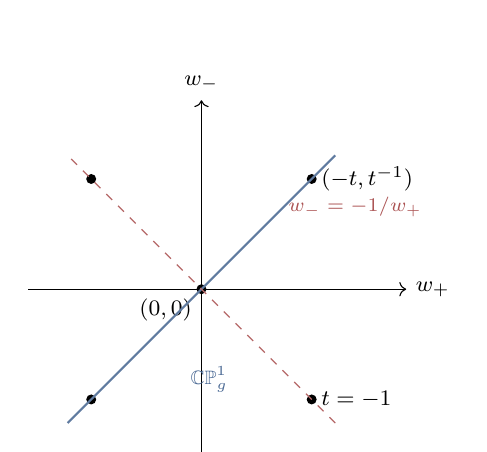
\begin{tikzpicture}[every node/.style={font=\footnotesize}]
\draw[->] (-2.2,0) -- (2.6,0) node[right] {$w_+$};
\draw[->] (0,-2.2) -- (0,2.4) node[above] {$w_-$};
\fill (0,0) circle (1.8pt); \node[below left] at (0,0) {$(0,0)$};
\fill (1.4,1.4) circle (1.8pt); \node[right] at (1.4,1.4) {$(-t,t^{-1})$};
\fill (-1.4,-1.4) circle (1.8pt);
\fill (1.4,-1.4) circle (1.8pt); \node[right] at (1.4,-1.4) {$t=-1$};
\fill (-1.4,1.4) circle (1.8pt);
\draw[kwblue!70,thick] (-1.7,-1.7) .. controls (-0.4,-0.4) and (0.4,0.4) .. (1.7,1.7);
\draw[kwred!70,dashed] (1.7,-1.7) -- (-1.7,1.7);
\node[font=\scriptsize,kwblue!80] at (0.1,-1.15) {$\mathbb{CP}^1_g$};
\node[font=\scriptsize,kwred!80] at (1.95,1.05) {$w_-=-1/w_+$};
\end{tikzpicture}
\caption{$\mathbb{CP}^1_g$（蓝曲线）落在二维参数空间 $\mathbb{CP}^1_h\times\mathbb{CP}^1_h$ 中；红虚线是 A-模型条件 $w_-=-1/w_+$，两者只在 $t$ 实（即 $w_-=-1/w_+$ 且 $w_+=-t$）时相交。}
\label{l1:fig:cpg}
\end{figure}

\begin{kcard}{§5.2 广义复几何：$\mathbb{CP}^1_g$ 与 $\Psi$（pp.65--70）}
\anchor{src p.65}

\noindent\textbf{① 这一节的任务}\quad 用广义复几何回答三个问题：$\mathbb{CP}^1_g$ 是什么、为什么它与 $C$ 的复结构无关、以及二维模型里 $\Psi$ 从哪来。\pA\anchor{src p.65}

\noindent\textbf{② 输入}\quad \S5.1 的 $(J_+,J_-)$；\S4.1 的 $\omega_I,\omega_J,\omega_K$ 与 $\Omega_J=\omega_K+\ii\omega_I$；\S3.5 的 $\Psi$。

\noindent\textbf{③ 关键构造}\quad
\begin{itemize}
\item 广义（殆）复结构。在 $TX\oplus T^*X$ 上取保持自然不定度规、平方为 $-1$ 的线性变换；可积者称广义复结构。两个基本例子：
\begin{equation}\tag{5.23--5.24}\label{l1:gb}
I_{\hat J}=\begin{pmatrix}\hat J&0\\0&-\hat J^t\end{pmatrix}\ (B\text{-模型}),\qquad
I_\omega=\begin{pmatrix}0&-\omega^{-1}\\ \omega&0\end{pmatrix}\ (A\text{-模型}) .
\end{equation}
$B$-场变换为 $I(B_0)=M(B_0)IM(B_0)^{-1}$，$M(B_0)=\begin{pmatrix}1&0\\B_0&1\end{pmatrix}$（原文 (5.25)--(5.26)）。\pA\anchor{src p.67}
\item 超凯勒情形。由 $(J_+,J_-)$ 给出的 $I_t$ 算得只依赖 $J$、$\omega_I$、$\omega_K$，等价地只依赖 $(J,\Omega_J)$；而 \S4.1 已证明这些与 $C$ 的度规/复结构无关，故 $\mathbb{CP}^1_g$ 族与 $C$ 的复结构无关。\pA\anchor{src p.68}
\item $\Psi$ 的二维解释。$I_t$（$t\ne\pm\ii$）等价于辛结构的 $B$-场变换，其复化 Kähler 类为
\begin{equation}\label{l1:bk}\tag{5.33}
[B_0+\ii\omega_0]=\frac{1}{\ii}\Im\tau\,\frac{t-t^{-1}}{t+t^{-1}}\,[\omega_I] ;
\end{equation}
加入 $\theta$ 项的贡献 $B'=-\Re\tau\,\omega_I$ 后
\begin{equation}\label{l1:psi2d}\tag{5.34}
[B+\ii\omega]=-[\omega_I]\,\Psi,\qquad
\Psi=\Re\tau+\ii\Im\tau\,\frac{t-t^{-1}}{t+t^{-1}} .
\end{equation}
\pA\anchor{src p.69}
\end{itemize}

\noindent\textbf{④ 结论}\quad
\begin{itemize}
\item $\Psi$ 在二维就是复化 Kähler 类 $[B+\ii\omega]$ 的系数；A-模型只依赖这个类，故理论只依赖 $\Psi$——这是 \S3.5 结论的二维重述。\pA\anchor{src p.69}
\item $t=\pm\ii$ 时上述分析失效（$B$-模型，$\Psi=\infty$），需单独论证与 $\tau$ 无关：$\Im\tau$ 控制 Kähler 类而 B-模型不看 Kähler 类，$\Re\tau$ 给 $B$-场加 $\omega_I$ 的倍数，但在 $B$-模型中 $(1,1)$ 与 $(2,0)$ 型 $B$-场的贡献可写成 $\{Q,\cdot\}$（$(0,2)$ 分量例外，它影响 B-膜范畴）。\pA\anchor{src p.70}
\item $B$-场含 $(2,0)\oplus(0,2)$ 分量时，纯全纯映射看不见它，但带膜时 A-膜条件 $F+B|_N=0$ 对全部分量敏感——这为 \S5.6 与 \S11 的膜讨论埋下伏笔。\pA\anchor{src p.70}
\end{itemize}

\noindent\textbf{⑤ 出口}\quad \S5.3 用 $\Psi=0,\infty$ 两点；\S5.4 在 $B(I)$ 模型中算 chiral ring；\S11.3 讨论一般 $\Psi$；\S11 的 D-模构造依赖 $\omega_I$ 的整性（\S4.1）。若没有 "$\Psi=[B+\ii\omega]$"，二维侧就只有一个抽象参数，无法与四维的 $\tau,t$ 对上。\pB\anchor{src p.70}

\noindent\textbf{⑥ 锚点索引}\quad
\begin{itemize}
\item p.65--67：广义复结构的定义、两个基本例子、$B$-场变换（原文 (5.23)--(5.26)）
\item p.68：$I_t$ 只依赖 $J,\omega_I,\omega_K$；$\mathbb{CP}^1_g$ 与 $C$ 的复结构无关
\item p.69：$\Psi$ 作为复化 Kähler 类（原文 (5.33)--(5.34)）
\item p.70：$t=\pm\ii$ 的 $\tau$ 无关性；$(0,2)$ 分量的作用
\end{itemize}
\end{kcard}

\noindent\stuck{为什么超凯勒流形上不必验证 $(2,2)$ 超对称的相容条件？因为超凯勒流形上任意一对 $(J_+,J_-)\in\mathbb{CP}^1_h\times\mathbb{CP}^1_h$ 给出的广义复结构都自动可积——Kähler 形式的封闭性提供了可积性。一般 target 上才需要 $[67]$ 的 $(2,2)$ 条件；本文只用到超凯勒情形，故"条件自动满足"。\pA\anchor{src p.68}}

\noindent\caveat{广义复几何在这一节是"语言"而非"定理"：作者明说"扭化 TFT 由其中一个广义复结构决定、另一个无关"是一个 belief（尚无完整证明，原文 p.66 的脚注语气）。不要把式 \eqref{l1:gb} 的对应当成已证等价；本解经本仅把它用作组织语言。\pA\anchor{src p.66}}

\begin{kcard}{§5.3 特殊化：$\Psi=0,\infty$ 与镜像对称（pp.70--72）}
\anchor{src p.70}

\noindent\textbf{① 这一节的任务}\quad 只取 $\Psi=\infty$（$t=\ii$，$J$ 的 B-模型）与 $\Psi=0$（其 S-对偶像，$K$ 的 A-模型），证明 S-对偶在这两点之间给出镜像对称，并列出所有模型的变换。\pA\anchor{src p.70}

\noindent\textbf{② 输入}\quad \S5.1 的 A/B 判据；\S5.2 的 $\Psi$；\S2.2 的 S 矩阵与相位。

\noindent\textbf{③ 关键构造}\quad
\begin{itemize}
\item 对偶群元素
\begin{equation}\label{l1:s2d}\tag{5.35}
S=\begin{pmatrix}0&1/\sqrt{n_g}\\-\sqrt{n_g}&0\end{pmatrix}:\quad \Psi\longmapsto-\frac{1}{n_g\Psi},
\end{equation}
交换 $\Psi=0$ 与 $\Psi=\infty$；$T$ 见原文 (5.36)。\pA\anchor{src p.71}
\item $\Psi=\infty$：$t=\ii\Rightarrow(w_+,w_-)=(-\ii,-\ii)$，即 $J$ 的 B-模型。施加 $S$（$\tau$ 仍取虚）得 $t'=1\Rightarrow(w_+,w_-)=(-1,1)$，即 $K$ 的 A-模型。故 S-对偶给出
\[
\MH(G,C)\text{ 的 }B(J)\ \Longleftrightarrow\ \MH(\Ldual,C)\text{ 的 }A(K).
\]
\pA\anchor{src p.71}
\item 复合 $I:\varphi\mapsto\ii\varphi$（把 $K$ 转回 $J$）得 $B(J)\leftrightarrow A(J)$，即 $\MH(G,C)$ 与 $\MH(\Ldual,C)$ 在复结构 $J$ 下互为镜像。但 $I$ 把 $A(J)$ 移出 $\mathbb{CP}^1_g$ 族，故这个"镜像"陈述需要额外一步。\pA\anchor{src p.71}
\item 全部模型的变换（原文 Table 2）：
\begin{center}\small
\begin{tabular}{@{}llll@{}}
\toprule
\tabhead{源模型} & \tabhead{像} & \tabhead{源模型} & \tabhead{像} \\
\midrule
$I$ 的 B & $I$ 的 B & $J$ 的 B & $K$ 的 A \\
$I$ 的 A & $I$ 的 A & $J$ 的 A & $K$ 的 B \\
$K$ 的 B & $J$ 的 A & $K$ 的 A & $J$ 的 B \\
\bottomrule
\end{tabular}
\end{center}
\pA\anchor{src p.72}
\end{itemize}

\noindent\textbf{④ 结论}\quad
\begin{itemize}
\item S-对偶保持 $B(I)$ 与 $A(I)$（由 $I$ 的 $U(1)_R$ 平庸性），交换 $B(J)\leftrightarrow A(K)$、$A(J)\leftrightarrow B(K)$。\pA\anchor{src p.72}
\item 镜像对称陈述：$\MH(G,C)$ 的 $B(J)$ 与 $\MH(\Ldual,C)$ 的 $A(J)$ 等价——这是几何 Langlands 的"物理半边"，其严格化（导出范畴等价）是 \S11 的内容。\pB\anchor{src p.71}
\item $\mathbb{CP}^1_g$ 内的对偶对是 $B(J)\leftrightarrow A(K)$；把它改写成 $B(J)\leftrightarrow A(J)$ 需要不自然的 $I$，这说明镜像对称的"自然"形式涉及 $K$ 而非 $J$。\pC\anchor{src p.72}
\end{itemize}

\noindent\textbf{⑤ 出口}\quad \S5.4 解释 S 为什么保持 Hitchin 纤维化（在 $B(I)$ 中论证、结论用于 $B(J)$ 与 $A(K)$）；\S5.5 用 SYZ 解释纤维上的 T-对偶；\S6 起所有线算子的词典都建立在这张表上。\pB\anchor{src p.73}

\noindent\textbf{⑥ 锚点索引}\quad
\begin{itemize}
\item p.70--71：$\Psi=\infty$ 与 $\Psi=0$ 的模型识别；$S$ 的作用（原文 (5.35)）
\item p.71--72：$I$ 的作用；$B(J)\leftrightarrow A(K)$ 与镜像陈述
\item p.72：Table 2 的六种变换
\end{itemize}
\end{kcard}

\noindent\stuck{为什么 $\Psi=\infty$ 取 $t=\ii$ 而不取 $t=-\ii$？二者给出同一理论（$t\sim-t$），取 $t=\ii$ 只是为使 $(w_+,w_-)=(-\ii,-\ii)$ 恰是 $J$ 的 B-模型；取 $-\ii$ 得到 $-J$ 的 B-模型，而 $\pm J$ 在 $\MH$ 上是同一个复结构。\pA\anchor{src p.62}}

\noindent\caveat{镜像对称的完整陈述是"$\MH(G,C)$ 与 $\MH(\Ldual,C)$ 的派生范畴等价"，本文只在 sigma 模型/膜的层面使用；且 $n_g=1$（simply-laced）时 $S$ 才精确是 $SL(2,\ZZ)$ 的 $S$，非单连通时 $\Gamma$ 是 Hecke 群，需用式 \eqref{l1:s2d} 的 $n_g$ 修正。\pB\anchor{src p.71}}

\begin{figure}[htbp]
\centering
\begin{tikzpicture}[every node/.style={font=\footnotesize},
  bx/.style={draw=kwblue!65,fill=kwboxbg,rounded corners=2pt,align=center,inner sep=4pt,text width=40mm}]
\node[bx] (g) {$\MH(G,C)$\\ $B(J)$（$\Psi=\infty$）};
\node[bx,right=22mm of g] (lg) {$\MH(\Ldual,C)$\\ $A(K)$（$\Psi=0$）};
\draw[<->,thick,kwred!80] (g) -- node[above] {$S$-对偶} node[below,font=\scriptsize] {镜像} (lg);
\node[bx,below=12mm of g] (gj) {$\MH(G,C)$\\ $A(J)$};
\node[bx,below=12mm of lg] (lgj) {$\MH(\Ldual,C)$\\ $B(K)$};
\draw[<->,thick,kwblue!80] (gj) -- node[above,font=\scriptsize] {$S$} (lgj);
\draw[-{Stealth},dashed] (g) -- node[right,font=\scriptsize] {$I$} (gj);
\draw[-{Stealth},dashed] (lg) -- node[right,font=\scriptsize] {$I$} (lgj);
\end{tikzpicture}
\caption{$\Psi=\infty$ 与 $\Psi=0$ 两点及 S-对偶。实线 $S$ 交换 $B(J)\leftrightarrow A(K)$；虚线 $I:\varphi\mapsto\ii\varphi$ 把它改写成镜像对称形式。}
\label{l1:fig:mirror}
\end{figure}

\begin{kcard}{§5.4 S-对偶与 Hitchin 纤维化（pp.72--75）}
\anchor{src p.72}

\noindent\textbf{① 这一节的任务}\quad 证明 S-对偶保持 Hitchin 纤维化：在底 $B$ 上给出经典的分级环同构，从而为"纤维上 T-对偶"的 SYZ 图像做准备。\pA\anchor{src p.72}

\noindent\textbf{② 输入}\quad \S4.3 的 $\pi:\MH\to B$ 与维数公式；\S5.2 的 $B(I)$ 模型；\S5.3 的 Table 2 与 \S3.5 的 canonical parameter——S-对偶在 $\Psi$ 上只是 $\Psi\mapsto-1/(n_g\Psi)$（式 \eqref{l1:s2d}），本节要证明它在整个底 $B$ 上是一个分级环同构，从而把"两个特殊点的对偶"提升为"整族对偶"。

\noindent\textbf{③ 关键构造}\quad
\begin{itemize}
\item 底 $B$ 上的函数。$\varphi$ 的基本齐次不变多项式 $P$ 与 $\alpha\in H^1(C,K_C^{1-\deg P})$ 给出交换 Hamilton 量
\begin{equation}\label{l1:hpa37}\tag{5.37}
H_{P,\alpha}=\int_C\alpha\,P(\varphi),
\end{equation}
它们在 $B$ 上给出全纯函数；$U\cong\CC^*$ 作用 $\varphi\mapsto\lambda\varphi$ 使其带权 $n=\deg P$。\pA\anchor{src p.72}
\item $B(I)$ 中的证明。$I$ 的 B-模型的 chiral ring 是 $\bigoplus H^q(\MH,\wedge^p T\MH)$，其 $(p,q)=(0,0)$ 部分即全纯函数环；$I$ 中紧 Hitchin 纤维上的全纯函数必为常数，故全纯函数环来自底 $B$。S 保持 $I$ 的 B-模型，故 S 诱导 $B(G)\to B(\Ldual)$ 的分级同构，并与两侧 $U(1)$ 作用相容。\pA\anchor{src p.73}
\item 4d 显式版本。在 $\RR^4$ 上定义 $D_n$：规范不变、在 $\varphi$ 中 $n$ 次齐次、且属 $SU(4)_R$ 的 $\mathrm{Sym}^n\mathbf 6$ 的多项式，即维数 $n$ 的半 BPS 局部算子；限制到 Weyl 腔最高权得 $D'_n$，其直和 $D'=\bigoplus D'_n$ 是规范理论的 chiral ring。S 与 $SU(4)_R$ 交换，故保持 $D'$，从而保持由它经 $\alpha$ 积分得到的 $H_{P,\alpha}$。\pA\anchor{src p.74}
\end{itemize}

\noindent\textbf{④ 结论}\quad
\begin{itemize}
\item S 把 $G$ 的 Hitchin 底映到 $\Ldual$ 的 Hitchin 底，并保持分级环结构与 $U(1)$ 作用；即 S 在底上是经典可计算的。\pA\anchor{src p.75}
\item S 不能由局部算子测得在纤维上的作用：局部算子只能"在 $z\in\Sigma$ 处求值"$H_{P,\alpha}$，即只看到底 $B$ 的信息；若 S 经典地作用在纤维上，就与"纤维上应为 T-对偶"矛盾——这正是 \S5.5 用 SYZ 补足的地方。\pA\anchor{src p.73}
\item 这个证明是"利用 $\MH$ 超凯勒性"的典型：论证在 $I$ 的 B-模型中进行，结论却用于 $J$ 的 B-模型与 $K$ 的 A-模型。\pA\anchor{src p.74}
\end{itemize}

\noindent\textbf{⑤ 出口}\quad \S5.5 的 SYZ 论证需要一个"底映射 $\Xi:B\to{}^LB$"与"纤维环面"的框架，本节提供前者；\S9--\S10 的 Hecke 算子在 Hitchin 纤维化上表现为谱曲线对应。若没有"底上经典、纤维上量子"的分工，镜像对称的 SYZ 陈述无从写出。\pB\anchor{src p.76}

\noindent\textbf{⑥ 锚点索引}\quad
\begin{itemize}
\item p.72：$H_{P,\alpha}$ 与 $B$ 的分级（原文 (5.37)）
\item p.73：$B(I)$ 中的 chiral ring 论证；局部算子只测底
\item p.74--75：$D_n$、$D'_n$ 与 4d 显式版本；S 保分级
\end{itemize}
\end{kcard}

\noindent\stuck{为什么"局部算子不能测纤维"是优点而非缺陷？因为若能用局部算子测纤维，S 就会经典地作用在纤维上，而 SYZ 镜像对称要求纤维上是 T-对偶（一种量子操作，翻转半径/复结构）。原文明确指出这一点，并把它与 \S5.5 的 SYZ 图像联系起来：底上经典、纤维上量子，正是镜像对称的标志。\pA\anchor{src p.73}}

\noindent\caveat{"S 在纤维上 T-对偶"不是本节证明的，本节只证底上的作用；纤维上的陈述由 \S5.5 的 SYZ 论证与数学结果（Hausel--Thaddeus 对 $U(N)$、Hitchin 对 $G_2$、Donagi--Pantev 对一般半单群）支持。不要把两者混成同一定理。\pB\anchor{src p.77}}

\begin{kcard}{§5.5 S-对偶的二维解释：SYZ（pp.75--78）}
\anchor{src p.75}

\noindent\textbf{① 这一节的任务}\quad 把 S-对偶解释为 Strominger--Yau--Zaslow 镜像对称：底上给映射 $\Xi:B\to{}^LB$，纤维上给环面 T-对偶。\pA\anchor{src p.75}

\noindent\textbf{② 输入}\quad \S5.3 的镜像对称；\S4.3 的纤维是复环面；\S5.2 的膜与 $(J_+,J_-)$。

\noindent\textbf{③ 关键构造}\quad
\begin{itemize}
\item 从 zerobrane 出发。$B_p$ 是支撑在 $p\in\MH(G,C)$ 的 zerobrane，对应边界条件"$\Phi$ 把边界映到 $p$"；点在任何复结构下都是复子流形，故 $B_p$ 是 $(B,B,B)$ 型。\pA\anchor{src p.76}
\item S-对偶像。Table 2 给出 $(B,B,B)\mapsto(B,A,A)$，故 $B_p$ 的对偶 $\tilde B_p$ 是 $I$ 中 B-膜、$J,K$ 中 A-膜。一般 A-膜至少中维，而 $\tilde B_p$ 的支撑至多中维，故它恰支撑在某条 Hitchin 纤维 $\tilde F=\Xi(F)$ 上；$I$ 中全纯、对 $\omega_J,\omega_K$ Lagrangian，加平坦酉 Chan--Paton 丛 $L$ 后正是 $(B,A,A)$ 型。\pA\anchor{src p.76}
\item 模空间比较。$B_p$ 的模空间是 $F$（$p$ 可在 $F$ 上变）；$\tilde B_p$ 的模空间是参数化 $\tilde F$ 上 rank-1 平坦 Chan--Paton 丛的复环面 $J_{\tilde F}$。rank 必须为 $1$（否则维数超出），且 $\dim J_{\tilde F}=\dim F$，故 $F\cong J_{\tilde F}$。\pA\anchor{src p.77}
\end{itemize}

\noindent\textbf{④ 结论}\quad
\begin{itemize}
\item S 作用 $=$ 底映射 $\Xi$（$\Ldual$ 与 $G$ 的 Hitchin 底之间的经典映射，simply-laced 时 $\Xi=\mathrm{id}$）$+$ 对应环面纤维上的 T-对偶。这正是 SYZ 镜像对称图像。\pA\anchor{src p.77}
\item 因而 $G$ 与 $\Ldual$ 的 Hitchin 纤维互为对偶复环面：$U(N)$ 由 Hausel--Thaddeus，$G_2$ 由 Hitchin，一般半单 $G$ 由 Donagi--Pantev（谱覆盖）。\pA\anchor{src p.78}
\item 省略的微妙处：$G$ 的中心与基本群（\S7 略述）、$C$ 上 spin 结构的作用（本文不分析）。\pA\anchor{src p.78}
\end{itemize}

\noindent\textbf{⑤ 出口}\quad \S5.6 用这套语言列出 MH 上的膜；\S6--\S8 把 Wilson/'t Hooft 线算子翻译成膜上的算子；\S9--\S10 的 Hecke 对应在纤维化上表现为谱曲线之间的对应。没有 SYZ 图像，"纤维上 T-对偶"就只是口头承诺。\pB\anchor{src p.78}

\noindent\textbf{⑥ 锚点索引}\quad
\begin{itemize}
\item p.75--76：zerobrane 与 $(B,B,B)$；S-对偶像为 $(B,A,A)$
\item p.77：支撑在纤维上；模空间比较给出 $F\cong J_{\tilde F}$
\item p.78：SYZ 结论；各群情形的数学出处；省略的微妙处
\end{itemize}
\end{kcard}

\noindent\stuck{为什么 rank 必须为 $1$？若 $\tilde B_p$ 携带 rank $r>1$ 的平坦 Chan--Paton 丛，其模空间维数至少是 $\dim\tilde F+(r^2-1)$，超过 $B_p$ 的模空间 $F$；而 S 是对合等价，两边的边界条件模空间必须逐点匹配，故只能 $r=1$。\pB\anchor{src p.77}}

\noindent\caveat{SYZ 图像通常假设底映射 $\Xi$ 平凡；这里 $\Xi$ 一般非平凡（simply-laced 时才是恒等）。因此本文的陈述是"$\Xi$ + 纤维 T-对偶"，比教科书版 SYZ 多一个底上的经典映射。\pA\anchor{src p.77}}

\begin{figure}[htbp]
\centering
\begin{tikzpicture}[every node/.style={font=\footnotesize}]
\node (bg) at (0,2.2) {$B$（$G$ 的 Hitchin 底）};
\node (bl) at (6.2,2.2) {${}^LB$（$\Ldual$ 的 Hitchin 底）};
\draw[-{Stealth}] (bg) -- node[above] {$\Xi$（经典）} (bl);
\node (fg) at (0,0) {$F$（复环面）};
\node (fl) at (6.2,0) {$\tilde F$（对偶复环面）};
\draw[-{Stealth}] (fg) -- node[above] {$T$-对偶（量子）} (fl);
\draw[-{Stealth},dashed] (fg) -- (bg); \draw[-{Stealth},dashed] (fl) -- (bl);
\draw[-{Stealth},dashed] (bg) -- node[left,font=\scriptsize] {$\pi$} (fg);
\end{tikzpicture}
\caption{SYZ 图像：底上 $\Xi$ 是经典映射，纤维上是环面 T-对偶。S-对偶 $=$ 这两部分的复合。}
\label{l1:fig:syz}
\end{figure}

\begin{kcard}{§5.6 MH 上的膜：类型与例子（pp.78--79）}
\anchor{src p.78}

\noindent\textbf{① 这一节的任务}\quad 系统列出 $\MH$ 上对各复结构 $I,J,K$ 有超对称性质的膜的类型与例子，为 \S6 起的"线算子 $=$ 膜算子"词典提供对象。\pA\anchor{src p.78}

\noindent\textbf{② 输入}\quad \S5.1 的 A/B 判据；\S5.3 的 Table 2；\S4.2 的复结构与稳定性。

\noindent\textbf{③ 关键构造}\quad
\begin{itemize}
\item 膜型。一个膜对每个复结构可以分别是 A 型或 B 型；最有趣者保留二维 sigma 模型的一半超对称（即四维理论的四分之一）。四类基本型：
\begin{center}\small
\begin{tabular}{@{}llll@{}}
\toprule
\tabhead{类型} & \tabhead{$I$} & \tabhead{$J$} & \tabhead{$K$} \\
\midrule
$(B,B,B)$ & B & B & B \\
$(B,A,A)$ & B & A & A \\
$(A,B,A)$ & A & B & A \\
$(A,A,B)$ & A & A & B \\
\bottomrule
\end{tabular}
\end{center}
\pA\anchor{src p.78}
\item 例子。zerobrane 是最显然的 $(B,B,B)$；空间填充膜（target 全 $\MH$，Chan--Paton 丛对三个复结构全纯）也是 $(B,B,B)$。$(B,A,A)$：$N$ 为 $I$ 中复子流形且对 $\Omega_I$（从而对 $\omega_J,\omega_K$）Lagrangian，加平凡 Chan--Paton 丛；例：Hitchin 纤维、固定 $E$ 而让 $\varphi$ 变的族。$(A,B,A)$/$(A,A,B)$：$J$ 或 $K$ 中的复 Lagrangian，例：固定 $A_z$（$J$ 情形）或固定 $A_z-\varphi_z$（$K$ 情形）而让另一支变的族。\pA\anchor{src p.79}
\end{itemize}

\noindent\textbf{④ 结论}\quad
\begin{itemize}
\item S 交换 $(B,B,B)\leftrightarrow(B,A,A)$，而 $(A,B,A)$ 与 $(A,A,B)$ 各自映到同型（Table 2）。\pA\anchor{src p.78}
\item 不存在 $(B,B,A)$ 型膜（$I,J$ 都全纯的子簇自动 $K$ 全纯），也不存在 $(A,A,A)$ 型。\pA\anchor{src p.79}
\item 更一般的膜：对 $I,J,K$ 的某个线性组合为 B 型、对与它正交的两个复结构为 A 型；\S11 的 coisotropic A-膜属于这一类，但支撑维数可高于中维。\pA\anchor{src p.79}
\end{itemize}

\noindent\textbf{⑤ 出口}\quad \S6 把 Wilson 与 't Hooft 线算子解释为作用在这四类膜上的算子；\S7--\S8 的 electric eigenbrane 是 $(B,A,A)$ 型；\S11 的 coisotropic A-膜构造 D-模范畴。若没有这张类型表，\S6 起的"词典"就无从编码。\pB\anchor{src p.79}

\noindent\textbf{⑥ 锚点索引}\quad
\begin{itemize}
\item p.78：四类基本膜型与超对称性质
\item p.79：各类例子；$(B,B,B)$ 的 zerobrane 与空间填充膜
\item p.79：不存在 $(B,B,A)$、$(A,A,A)$；coisotropic 膜的预告
\end{itemize}
\end{kcard}

\noindent\stuck{为什么 $(B,A,A)$ 的支撑必须既是 $I$-复子流形、又对 $\Omega_I$ Lagrangian？"$I$ 中 B-膜"要求支撑 $N$ 在 $I$ 下复；"$J,K$ 中 A-膜"要求 $N$ 对 $\omega_J,\omega_K$ Lagrangian。而 $\Omega_I=\omega_J+\ii\omega_K$ 是 $I$ 的全纯辛形式，在复子流形 $N$ 上 $\Omega_I|_N$ 的消失恰等价于两个实辛形式同时拉回为零。所以三个条件其实是"$N$ 是 $\Omega_I$-Lagrangian"的分解表述。\pA\anchor{src p.79}}

\noindent\caveat{四类基本型不是全部膜。更一般的膜对 $I,J,K$ 的某个线性组合是 B 型；\S11 的 coisotropic A-膜支撑维数可高于中维，不能塞进这张表。本表只覆盖"保留一半 2d 超对称"的重要膜。\pA\anchor{src p.79}}

\subsection*{本节锚点索引}

下表汇总本文件用到的全部原文锚点（印刷页 $N$ 对应 \texttt{p\{$N+1$:03d\}.txt}），第三列是一句话内容。

\begin{longtable}{@{}llp{9.4cm}@{}}
\toprule
\tabhead{锚点} & \tabhead{印刷页} & \tabhead{内容} \\
\midrule
\endhead
\bottomrule
\endfoot
\S2 开篇 & p.6 & $\mathcal N=4$ 由十维降维；G 取紧致、$G_{\CC}$ 为其复化 \\
十维场内容 & p.7--8 & $\Gamma$、手征条件、$A$ 与 $\lambda$ 的反厄米约定 \\
$I_4$ 与 $\theta$ 项 & p.9 & 降维后的四维作用量（原文 (2.10)--(2.11)）\\
$\tau$ 与超代数 & p.10--11 & $\tau$ 的定义（2.12）、$SU(4)_R$、式 (2.15) \\
S-对偶 & p.11--12 & 猜想、$SL(2,\ZZ)$、$S$ 矩阵 (2.16)、$n_g$ \\
手征相位 & p.13--14 & S 与超荷的相位；$\hat\varphi$ 在 Coulomb 分支确定 \\
中心荷 & p.15 & $Z$ 的变换（2.22）与 $SL(2,\ZZ)$ 作用 \\
相位平方根 & p.16 & $\ee^{-\ii\hat\varphi}$ 的双覆盖（2.25）\\
扭化 & p.17--19 & 三种扭化、$\kappa$、$\mathbf 4$ 与 $\mathbf 6$ 的分解、$K$ 与 $\sigma$ \\
超荷族 & p.21--23 & 不变超荷、$K=\Gamma_{89}$（3.11）、$t$ 与 $t\sim-t$（3.13)--(3.14) \\
一族 A-模型 & p.25--27 & $Q$-不变方程 (3.29)；$t=\pm\ii$ 的平坦性；上同调场论解释 \\
消失定理 & p.28--31 & 定理 1、1$'$、2；恒等式 (3.32)--(3.34)；$\Sigma\times C$ 推论 \\
拓扑拉氏量 & p.31--35 & $\delta_t$ 代数、辅助场、$I_0,I_1,I_2$（3.49）\\
典范参数 & p.35--38 & $\Psi$ 的定义 (3.50)；特殊值 (3.52)；S-对偶作用 (3.53)--(3.54)；定向反转 \\
紧化与 Hitchin 方程 & p.38--40 & $M=\Sigma\times C$；Hitchin 方程 (4.1) \\
$\MH$ 的超凯勒商 & p.40--46 & $W$ 的度规 (4.2)、$I_w$ (4.6)--(4.7)、辛形式 (4.8)--(4.10)、矩映射 (4.11) \\
度规与 $B$-场 & p.47--49 & 物理诱导度规 (4.15)、$B=-\Re\tau\,\omega_I$ (4.19) \\
复结构 $I$ & p.49--51 & $I$ 中的 Hitchin 对 (4.20)；稳定性 \\
复结构 $J$ & p.51--53 & 平坦 $\gC$ 联络与同态 (4.21)--(4.22)；$I_w$ 等价性；$U(1)$ 作用 (4.23) \\
纤维化与可积性 & p.53--56 & $T^*\mathcal M\subset\MH$、$B$ 与 $d_i$ (4.24)--(4.25)、Hamilton 量 (4.26)、复环面纤维 \\
二维 TFT 开篇 & p.56--58 & (5.1)--(5.4)；(4,4) 超对称的二维结构 \\
扭化 TFT & p.58--61 & $(J_+,J_-)$ 与 (5.5)--(5.6)；A/B 判据 \\
4d 参数的二维像 & p.61--63 & $(w_+,w_-)=(-t,t^{-1})$ (5.11)、$q=-t^2$ (5.12)、$\mathbb{CP}^1_g$ 为子族 \\
4d 解释与 S-对偶 & p.63--65 & $(\hat u',\hat v')$ 分解；S 对 $w_\pm$ 的相位作用 (5.22) \\
广义复几何 & p.65--67 & 定义；(5.23)--(5.26)；$(2,2)$ 条件与扭化 TFT 的对应（belief）\\
$\mathbb{CP}^1_g$ 的无关性 & p.67--68 & $I_t$ 只依赖 $J,\omega_I,\omega_K$ \\
$\Psi$ 的二维解释 & p.69--70 & (5.33)--(5.34)；$B$-场 $(0,2)$ 分量与 A-膜条件 \\
$\Psi=0,\infty$ & p.71--72 & $S$ 矩阵 (5.35)、$T$ (5.36)；$B(J)\leftrightarrow A(K)$；Table 2 \\
S 与纤维化 & p.72--75 & $H_{P,\alpha}$ (5.37)；$B(I)$ 中的 chiral ring；$D_n$ 与 $D'_n$ \\
SYZ & p.75--78 & zerobrane 到 $(B,A,A)$；$F\cong J_{\tilde F}$；各群情形的数学结果 \\
膜的分类 & p.78--79 & 四类基本膜型；例子；不存在 $(B,B,A)$、$(A,A,A)$ \\
\end{longtable}



% ======================================================================
%  21_layer1_geom.tex — 结构层（下）：§6–§12 的结构卡
%  只写正文，preamble 由 main.tex 提供；严格按 plan/01 §5 六栏卡格式。
%  所有锚点页码均为印刷页码 N（正文在 source/text/p{N+1:03d}.txt）。
% ======================================================================

% 本节局部记号（preamble 不改）：对偶群的权与表示记为 ^L w、^L R。

\section{结构层（下）：从膜算子到 $D$-模翻译器（\S6--\S12）}

\subsection{\S6--\S12 总述：一条四段链、三种可信度}

结构层上半（\S2--\S5）拆的是机器：如何把 $N=4$ 超对称 Yang--Mills 扭化成 4d 拓扑场论，如何在
Riemann 面 $C$ 上紧化得到 $\MH$ 上的 2d 拓扑 sigma 模型，以及这个模型里"膜"是什么意思。下半
（\S6--\S12）拆的是用法：把这台机器对准几何 Langlands 的两个方向。与上半不同，这七节不是七个并列
话题，而是一条递进链；每一节的输出是下一节的输入，任何一环断掉，几何 Langlands 的标准陈述就拼不
起来。本节给这七节各画一张结构卡，并在每张卡上标出：哪些陈述是原文的硬结论（A），哪些是物理上自
然而原文一句话带过的推断（B），哪些是作者自己说 "we expect / we believe" 的猜想（C）。

\begin{keyidea}
\textbf{链条一句话}：\S6 把 4d 线算子变成 2d 膜范畴的自函子（骨架 S5）；\S7--\S8 证明电特征膜就是
同态 $\pi_1(C)\to\LdualC$，其中 \S7 的 flux 修正不可省（S6）；\S9--\S10 证明 't Hooft 算子的作用
恰好是 Hecke 修改（S7）；\S11--\S12 用典范余各向同性 A-膜把 magnetic 侧翻译成 $D$-模，得到几何
Langlands 的标准形式（S8）。
\end{keyidea}

\textbf{(1) S5，\S6：线算子 $=$ 膜算子。}这一步的真正发明不是"线算子存在"（任何规范理论都有 Wilson
线），而是\textbf{把线算子当成作用在膜范畴上的算符}，并因此只能说"特征值是向量空间"：$XB\simeq B\otimes V$
\pA\anchor{src p.95}。没有这个升级，"本征值"就只是数，几何 Langlands 里的 eigensheaf（特征层）在物理
侧没有对应物。4d 来源还白送两个结构：线算子自动交换，因此可以同时对角化；特征值 $V_p$ 随 $p\in C$
成为平坦丛，已经预演了"局部系统"。

\textbf{(2) S6，\S7--\S8：电特征膜 $=\pi_1(C)$ 的表示。}物理侧 \S8.2 只用一行计算——任意向量丛在
一点处平凡——就得到：位于 $x\in\MH$ 的 zerobrane 是电特征膜，特征值是 $E_q(R)|_x$ \pA\anchor{src p.121}。
但 \S7 必须插在中间，因为 universal $G$-bundle 不存在，Chan-Paton 丛只能是 twisted 的，离散电
flux $e_0$ 恰好就是 twist 的标签；正确的物理对象是"所有 $e_0$ 的 twisted zerobrane 之和" \pA\anchor{src p.122}。
删掉 \S7，\S8.2 的"特征值"在 $e_0\ne0$ 时根本没有意义。这是七节链里最容易被数学读者误判为"背景复
习"的一节。

\textbf{(3) S7，\S9--\S10：'t Hooft $=$ Hecke。}\S9.1 对 $U(N)$ 把 't Hooft 算子的奇点逐分量解出来，
得到 $L_i\mapsto L_i\otimes\mathcal O(p_0)^{m_i}$，这就是 Hecke 修改的定义式 \pA\anchor{src p.132}。
\S9.2--\S9.3 说明"所有可能的 Hecke 修改"构成仿射 Grassmannian 的变体；\S10 用 Bogomolny 方程把这
个空间实现成边界条件的模空间，并在 \S10.4 算出 't Hooft 算子的 OPE。这一步补上了磁侧缺失的表示论：
Wilson 有现成的 $\mathrm{Rep}(G)$，而 't Hooft 的代数结构必须由 Hecke 修改空间的几何给出。

\textbf{(4) S8，\S11--\S12：$D$-模翻译器。}\S11.1 在 $\MH$ 上造出典范余各向同性 A-膜，\S11.2 说明
A-膜给出 $\MC$ 上的 $D$-模；于是 \S8.2 的 type F 膜（magnetic eigenbrane）对应 $D$-模，正是几何
Langlands 的标准陈述。\S12 不是新定理：它把全篇的膜放进一张按三个复结构分类的检查清单，供读者核对
每种膜落在 GL 的哪一边。因此 \S12 的卡片要点不是"得到结论"，而是"如何不重不漏地列举膜"。

\paragraph{与 \S2--\S5 的文本差异：数学读者必须换一种读法。}
上半的 A 级陈述（扭化、超凯勒商、Hitchin 纤维化的 T-对偶）基本可以当定理读；下半的 A 级陈述要打
折，因为整条链建立在两个物理前提上：(i) $N=4$ 超对称 Yang--Mills 的 S-对偶本身是一个有强证据但未
证明的猜想，原文在 \S2.2 把它当作已建立的事实使用 \pA\anchor{src p.11}；(ii) 4d 拓扑场论的存在与
拓扑性来自 \S3 的物理构造，其中 \S3.3 的消失定理只在附加条件下成立 \pA\anchor{src p.28}。所以本书
标 A 的准确含义是"原文明确写出、且我们核验了其推理"，不是"数学上已被证明"。下半真正的"猜点"集中在
以下几处，读到那里应放慢：

\begin{table}[htbp]
\centering\small
\begin{tabular}{@{}p{1.85cm}p{5.1cm}p{8.45cm}@{}}
\toprule
\tabhead{位置} & \tabhead{原文语气} & \tabhead{读者要小心什么} \\
\midrule
\S6.4 & "we expect"（(6.28)--(6.29)） & 't Hooft 算子的 OPE 没有物理侧的直接计算，作者只从 Coulomb 分支读出最高权部分，其余交给 \S10.4 的 Hecke 修改空间几何 \pC\anchor{src p.99} \\
\S9.2 & "we will see / it is natural" & Hecke 修改空间的连通性与维数依赖单极子解的存在性；数学上这是已知定理，但物理侧是重建 \pB\anchor{src p.135} \\
\S10.2 & "monopole bubbling" & 单极子成泡的图像是半经典推断，原文用它解释 Hecke 空间的奇点 \pC\anchor{src p.155} \\
\S11.2 & "we argue / we believe" & A-膜 $\leftrightarrow$ $D$-模的对应是启发式论证，不是范畴等价的证明 \pC\anchor{src p.196} \\
\S12 & "we expect / we believe" & 三种膜型的清单是物理分类，其完备性没有独立证明 \pC\anchor{src p.207} \\
\bottomrule
\end{tabular}
\caption{后半程的"猜点"清单。标 C 的断言在正文卡片里都会再次点明，不要把它们当定理引用。}
\label{tab:geom-guesses}
\end{table}

\begin{figure}[htbp]
\centering
\begin{tikzpicture}[node distance=5mm and 5mm, box/.style={draw=kwblue!65, fill=kwblue!4,
  rounded corners=2pt, align=center, font=\small, inner sep=4pt, text width=3.25cm}]
\node[box] (s5) {\textbf{S5}（\S6）\\ 线算子 $=$ 膜算子\\[2pt]
  {\scriptsize 输出：自函子 $X$、$XB=B\otimes V$}};
\node[box, right=of s5] (s6) {\textbf{S6}（\S7--\S8）\\ 电特征膜\\[2pt]
  {\scriptsize 输出：$\pi_1(C)\to\LdualC$ 的表示}};
\node[box, right=of s6] (s7) {\textbf{S7}（\S9--\S10）\\ 't Hooft $=$ Hecke\\[2pt]
  {\scriptsize 输出：Hecke 算子代数}};
\node[box, right=of s7] (s8) {\textbf{S8}（\S11--\S12）\\ c.c.\ A-膜 $\to$ $D$-模\\[2pt]
  {\scriptsize 输出：GL 标准形式}};
\draw[-{Latex[length=2mm]}] (s5) -- node[above,font=\scriptsize]{Wilson} (s6);
\draw[-{Latex[length=2mm]}] (s6) -- node[above,font=\scriptsize]{对偶} (s7);
\draw[-{Latex[length=2mm]}] (s7) -- node[above,font=\scriptsize]{magnetic} (s8);
\end{tikzpicture}
\caption{后半程的四段链。箭头上的词是"上一段的输出被下一段消费的部分"；每段内部还可细分：\S7 是
\S8 的修正项，\S10 是 \S9 的几何实现，\S12 是 \S11 的分类清单。}
\label{fig:geom-chain}
\end{figure}

% ======================================================================
\subsection{\S6 圈与线算子：从 4d 算子到 2d 膜范畴（pp.78--102）}

\S6 是后半程的入口，也是全文语气转折的地方：从这里开始作者不再造理论，而是让理论去作用。本节的
输出是骨架 S5——4d 拓扑场论的线算子给出 2d 膜范畴的自函子，特征对象（eigenbrane）的"特征值"是一个
向量空间。这一步的输入是 \S3 的标量超荷与扭化参数、\S4 的 $\MH$ 三复结构、\S5 的膜范畴；出口分三
路：\S7--\S8 修正并具体化电特征膜，\S9--\S10 具体化磁侧的 Hecke 作用，\S11 要用的"magnetic
eigenbrane 带平坦丛"也在本节末尾就位。

\S6 内部四小节的逻辑是：先造两种基本算子（Wilson 在 $\Psi=\infty$，'t Hooft 在 $\Psi=0$，混合算子
在有理 $\Psi$），再把它们紧化到 2d 并翻译成"作用在膜上"，最后定义 eigenbrane 并证明 4d 来源给出的
两个自动性质。注意 6.1 与 6.2 的对称性：Wilson 的做法是"把 $\varphi$ 加进联络"，'t Hooft 的做法是
"让 $\varphi$ 跟着奇点发散"；两者都是为了让同一个标量超荷 $Q$ 存活。

\begin{kcard}{\S6.1 拓扑 Wilson 算子（pp.79--80）}
\begin{enumerate}[label=\textbf{\arabic*}]
\item \textbf{这一节的任务}：在 $\Psi=\infty$（即 $t=\pm\ii$）构造保持拓扑超荷 $Q$ 的 Wilson 线算子，
  并说明为什么普通的 $W_0(R,S)=\Tr_R P\exp(-\oint_S A)$ 不够、必须把规范场替换成
  $\mathcal A=A+\ii\varphi$。
\item \textbf{输入}：\S3.1 的拓扑变换 (6.2)--(6.3)；骨架 S2（存在标量超荷 $Q$）、S3（$M=\Sigma\times C$
  与 $\MH$ 的几何）。
\item \textbf{关键构造}：普通 Wilson 圈在拓扑变换 $A_\mu\mapsto A_\mu+\ii u\psi_\mu+\ii v\tilde\psi_\mu$
  下不变；但 Higgs 场按 $\delta_T\varphi_\mu=\ii v\psi_\mu-\ii u\tilde\psi_\mu$ 变换，两者在
  $t=v/u=\pm\ii$ 时的组合不变：
\begin{equation}
\begin{aligned}
W(R,S)&=\Tr_R P\exp\Big(-\oint_S (A+\ii\varphi)\Big) &&(t=\ii),\\
W(R,S)&=\Tr_R P\exp\Big(-\oint_S (A-\ii\varphi)\Big) &&(t=-\ii).
\end{aligned}
\label{eq:geom-wilson}
\end{equation}
  开线情形的 $W(R,S)$ 不是迹，而是从 $p$ 到 $q$ 的平行移动矩阵 \pA\anchor{src p.79}\anchor{src p.80}。
\item \textbf{结论}：Wilson 算子是 $\Psi=\infty$ 处保持拓扑对称的线算子，按 $G$ 的不可约表示 $R$ 分类；
  其存在性的一句话解释是：$t=\pm\ii$ 的拓扑方程断言 $\mathcal A$ 平展，故沿闭圈的 holonomy 是自然
  不变量 \pA\anchor{src p.80}。
\item \textbf{出口}：\S8.1 要把这个算子对膜的作用算成 Chan-Paton 丛的张量积；为此所需的"$\varphi$ 的
  费米补偿"正是 \eqref{eq:geom-wilson} 里 $\ii\varphi$ 的 2d 对应物 \pB\anchor{src p.119}。
\item \textbf{锚点索引}：p.79 定义 $W_0(R,S)$ 与符号约定；p.80 变换律 (6.2)--(6.3) 与 $t=\pm\ii$ 的
  组合；p.80 开线算子 $=$ 平行移动矩阵；p.80 拓扑方程 $\Rightarrow$ 平展性。
\end{enumerate}
\textbf{可信度}：公式与变换律是 A。"在 $t=\pm\ii$ 存在极自然"是作者的物理判断（B），依据只有平展性；
"对一般 $t$ 不存在"作者自己加了限定——\S3.3 的消失定理需要全局输入、对有膜的场合不一定成立
\pB\anchor{src p.80}。
\end{kcard}

\begin{kcard}{\S6.2 拓扑 't Hooft 算子（pp.81--85）}
\begin{enumerate}[label=\textbf{\arabic*}]
\item \textbf{这一节的任务}：构造 Wilson 算子在 S-对偶下的对象——'t Hooft 算子，并确定它在 $\Psi=0$
  保持 $Q$ 所需的场奇点。这是"序算子 $\leftrightarrow$ 无序算子"在拓扑理论中的实现。
\item \textbf{输入}：\S2.2 的 S-对偶 $S:\Psi\mapsto-1/n_g\Psi$；\S6.1 的 Wilson 算子；GNO 对偶
  （`\S\S1` 想法 3 的算子版）。
\item \textbf{关键构造}：$U(1)$ 情形取 Dirac 单极奇点
\begin{equation}
F=\frac{\ii}{2}\,\star_3 \dd\frac{1}{r},\qquad
\varphi=\frac{\ii}{2|\vec x|}\,\dd s ,
\label{eq:geom-thooft}
\end{equation}
  其中 $\star_3$ 是法向 $\RR^3$ 的 Hodge 星、$\dd s$ 是沿线方向的标架；带电荷 $m$ 时整体系数乘 $m$。
  一般 $G$ 用同态 $\rho:U(1)\to G$（共轭类 $=$ $\Ldual$ 的最高权 $=$ $\Ldual$ 的不可约表示）嵌入
  \eqref{eq:geom-thooft}，得到算子 $T(\LR,S)$ \pA\anchor{src p.83}\anchor{src p.84}。
\item \textbf{结论}：'t Hooft 算子按 $\Ldual$ 的不可约表示分类（GNO 对偶的算子版）；其奇点携带特征
  类 $\xi(\LR)\in H^2(S^2,\pi_1(G))$，拓扑非平凡当且仅当 $\Ldual$ 的中心在 $\LR$ 上非
  平凡地作用 \pA\anchor{src p.84}。
\item \textbf{出口}：\S9.1 把这个奇点逐分量解出来，发现它的效果恰好是 Hecke 修改；\S8.1 用 $\xi(\LR)$
  写出 't Hooft 算子如何改变 $m_0$ \pA\anchor{src p.120}。
\item \textbf{锚点索引}：p.81 't Hooft 作为 disorder 算子的定义（法丛定向）；p.82--p.83 单极奇点与
  Maxwell 方程；p.83 (6.9) 保持拓扑对称的 $\varphi$ 奇点；p.84 $\rho:U(1)\to G$、GNO 分类、与
  $\PP^1$ 上 $G$-丛分类的关系。
\end{enumerate}
\textbf{可信度}：奇点公式与 GNO 分类是 A（引 [10],[90]）。"$\PP^1$ 上 $G$-丛的 Grothendieck 分类
解释 't Hooft 算子"是 B：论证依赖"$\PP^1$ 上 Yang--Mills 解都等价于阿贝尔解"这一物理陈述
\pB\anchor{src p.84}。而"$\Psi=0$ 必有对偶算子"本身依赖 S-对偶（见总述），属于条件性的 A。
\end{kcard}

\begin{kcard}{\S6.3 紧化到二维（pp.89--92）}
\begin{enumerate}[label=\textbf{\arabic*}]
\item \textbf{这一节的任务}：确定 4d 线算子紧化到 $\Sigma$ 之后在 2d 有效理论里的身份——答案是把线
  算子翻译成"边界条件/膜"，这是全篇"算子作用于膜"的语言基础。
\item \textbf{输入}：S3（$M=\Sigma\times C$ 紧化）；\S6.1--\S6.2 的两种算子；\S5 的膜与 $(B_1,B_2)$
  开弦空间。
\item \textbf{关键构造}：按曲线 $S\subset\Sigma\times C$ 的形状分三类：(a) $S=p\times S'$（在 $C$ 内绕
  圈）在 2d 中是点状局部算子；(b) $S=S''\times q$（沿 $\Sigma$ 走）仍是线算子；(c) 一般曲线同伦于
  "在 $\Sigma$ 上走、间或在 $C$ 中绕圈"，故是线算子加上插在特殊点的局部算子 \pA\anchor{src p.89}\anchor{src p.90}。
  关键的折叠（folding）技巧：一条线算子把平面分成两个区域 $Y$ 与 $Z$，把 $Z$ 的定向翻转后折叠，
  线算子变成 $Y\otimes Z$ 中的边界条件，即 $(Y,Z)$-膜 \pA\anchor{src p.90}。由此引出
  $H_{B_1,B_2}$（$(B_1,B_2)$ 开弦空间）、拼接乘法 $H_{B_1,B_2}\otimes H_{B_2,B_3}\to H_{B_1,B_3}$，
  以及 $H_{B,B}$ 的结合代数结构 \pA\anchor{src p.91}。
\item \textbf{结论}：在 2d 中"线算子 $=$ 作用在膜上的算符"有了严格含义：$X$ 把 $B$ 变成新膜 $XB$；
  边界上的局部算子空间就是 $H_{B,B}$，而 $H_{B,\tilde B}$ 是 $(H_{B,B},H_{\tilde B,\tilde B})$ 双模
  \pA\anchor{src p.92}。
\item \textbf{出口}：\S6.4 的 eigenbrane 定义只需要这一节的"$X$ 可以作用在 $B$ 上"；\S8.1 则反过来
  用 2d 边界项的 holonomy 与 4d Wilson 线比较。
\item \textbf{锚点索引}：p.89 图 4 的三种曲线；p.90 折叠技巧与 $(Y,Z)$-膜；p.91 图 6 的拼接与结合律；
  p.92 边界局部算子 $=H_{B,B}$、双模结构。
\end{enumerate}
\textbf{可信度}：几何分解与折叠技巧是 A（原文写得完整，技巧引 [93--95]）。"$H_{B,B}$ 是结合代数"
是 TQFT 公理的直接应用，数学上是标准的（A）；但"边界局部算子空间 $=H_{B,B}$"的切割论证是物理图
像（B，见图 6(d) 的解释）\pB\anchor{src p.92}。
\end{kcard}

\begin{figure}[htbp]
\centering
\begin{tikzpicture}[font=\small,
  box/.style={draw=kwblue!65, fill=kwblue!4, rounded corners=2pt, align=center,
    inner sep=4pt, text width=3.4cm}]
\node[box] (op) {4d：线算子 $X$\\ 支撑在 $S\subset M$};
\node[box, right=1.2cm of op] (br) {2d：边界条件\\（膜 $B$）};
\node[box, right=1.2cm of br] (nb) {新膜 $XB$\\（$X$ 贴近边界）};
\draw[-{Latex[length=2mm]}] (op) -- node[above,font=\scriptsize]{紧化} (br);
\draw[-{Latex[length=2mm]}] (br) -- node[above,font=\scriptsize]{作用} (nb);
\node[draw=kwred!60, rounded corners=2pt, inner sep=4pt, font=\scriptsize,
  below=9mm of br, text width=6.2cm] (eig) {特征膜：$XB\simeq B\otimes V$，
  {\normalfont 特征值不是数而是向量空间 $V$}};
\draw[-{Latex[length=1.6mm]}, kwred!60, dashed] (nb.south) to[out=-90,in=0] (eig.east);
\end{tikzpicture}
\caption{线算子的两级翻译：先把 4d 线算子紧化成 2d 边界条件，再让它在膜上作用。第二级翻译是 \S6
的中心思想，也是"特征值升级为向量空间"的来源。}
\label{fig:geom-op-brane}
\end{figure}

\begin{kcard}{\S6.4 边界附近的线算子与 eigenbrane（pp.93--102）}
\begin{enumerate}[label=\textbf{\arabic*}]
\item \textbf{这一节的任务}：定义线算子作用在膜上（$B\mapsto XB$）与 eigenbrane（$XB=B\otimes V$），
  并证明"来自 4d"给 eigenbrane 带来两个自动结构：算子族自动交换、特征值随 $p\in C$ 构成平坦丛。
\item \textbf{输入}：\S6.3 的膜作用；\S5 的膜范畴；S3（线算子来自 4d，故可定义在任意 $p\in C$ 处）。
\item \textbf{关键构造}：线算子 $X$ 贴近边界时把边界条件 $B$ 变成有效边界条件 $XB$（p.94）；
  张量积 $B\otimes V$ 由 $H_{\tilde B,B\otimes V}=H_{\tilde B,B}\otimes V$ 刻画；于是
\begin{equation}
XB\simeq B\otimes V \qquad\text{（eigenbrane 的定义，对应 Beilinson--Drinfeld 的 eigensheaf）}.
\label{eq:eigenbrane}
\end{equation}
  两个算子交换的定义是 $X_1X_2B=X_2X_1B$（对一切 $B$），交换则可同时对角化；来自 4d 的线算子自动
  交换（论证见原文脚注 31：两算子的支撑点可在 $C$ 中分开、不产生奇点）。特征值随 $p$ 变化：
  $X_pB=B\otimes V_p$，且移动 $p$ 等价于改变 $C$ 的度量、只差 BRST 平凡项，故 $V_p$ 上有一个平坦
  联络——$V_p$ 是 $C$ 上平坦丛的纤维 \pA\anchor{src p.93}\anchor{src p.95}\anchor{src p.96}\anchor{src p.97}。
\item \textbf{结论}：\textbf{electric eigenbrane} 是 Wilson 算子族的联合特征膜，\textbf{magnetic
  eigenbrane} 是 't Hooft 算子族的；$S$ 交换二者，并交换两种膜的超对称型；(B,B,B) 与 (B,A,A) 的
  Wilson/'t Hooft 特殊线算子分别对应（见下卡）\pA\anchor{src p.97}\anchor{src p.98}。Wilson 算子族的
  OPE 就是 $G$ 的表示环（$R\otimes\tilde R=\oplus_\alpha n_\alpha R_\alpha$ 给出逐项乘积）；
  't Hooft 算子族的 OPE 与 $\Ldual$ 的表示环同构——\textbf{但这一步原文是猜的}
  \pC\anchor{src p.98}\anchor{src p.99}。
\item \textbf{出口}：\S8.2 把 zerobrane 具体地认成 electric eigenbrane；\S9--\S10 证明 't Hooft 族
  的作用 $=$ Hecke 算子族，从而把上式中的"交换代数"落实为 Hecke 算子代数。
\item \textbf{锚点索引}：p.94 $B'=XB$；p.95 (6.22) eigenbrane 定义；p.95--p.96 张量积与 eigensheaf；
  p.97 (6.25) 平坦丛与脚注 31 的交换性论证；p.98 (6.27) Wilson OPE；p.99 (6.29) 't Hooft OPE
  的期望；p.101 线算子 $=$ 膜范畴的自函子；p.102 special Wilson 的 (B,B,B) 型。
\end{enumerate}
\textbf{可信度}：定义与 Wilson OPE 是 A；"4d 来源 $\Rightarrow$ 自动交换"是 A$^-$——论证只在 $C$
至少二维时成立，作者自己指出这一点 \pB\anchor{src p.97}；'t Hooft OPE (6.29) 是 C：原文说
"we expect"，并明确承认物理文献没有直接计算过 't Hooft 算子的 OPE，只从 Coulomb 分支读出最高权
项，其余交给 \S10.4 \pC\anchor{src p.99}。special Wilson/'t Hooft 的 (B,B,B)/(B,A,A) 型是 A
（由 (6.30)--(6.31) 与 \S5.3 表 2 得到）\pA\anchor{src p.102}。
\end{kcard}

\begin{figure}[htbp]
\centering
\begin{tikzpicture}[font=\small, every node/.style={align=center}]
\node (I) at (90:2.05) {\textbf{复结构 $I$}};
\node (J) at (210:2.05) {\textbf{复结构 $J$}};
\node (K) at (330:2.05) {\textbf{复结构 $K$}};
\draw[kwblue!60, thick] (J) -- (I);
\draw[kwblue!60, thick] (I) -- (K);
\draw[kwblue!60, thick] (J) -- (K);
\node[font=\scriptsize, text width=4cm, above=2mm of I] {(B,B,A) 与 (A,A,A) 不存在};
\node[draw=kwblue!65, fill=kwblue!4, rounded corners=2pt, inner sep=3pt,
      text width=5.0cm, anchor=west, font=\scriptsize] at (3.6,0.1)
  {允许的四类词：\\
   (B,B,B)：0-膜、space-filling 膜\\
   (B,A,A)：Hitchin 纤维、$I$ 中复拉格朗日（$\Omega_I$ 全纯辛）\\
   (A,B,A)/(A,A,B)：$J/K$ 中复拉格朗日（$\omega_J,\omega_K$）};
\end{tikzpicture}
\caption{膜类型的三角关系：一个膜在三个复结构 $I,J,K$ 上分别取 B 型或 A 型，构成一个三位词。物理上
允许的是 (B,B,B)、(B,A,A)、(A,B,A)、(A,A,B)；若一个子流形在 $I,J$ 上全纯，则自动在 $K$ 上全纯，
故 (B,B,A) 不存在。special Wilson 线 $=(B,B,B)$，special 't Hooft 线 $=(B,A,A)$，$S$-对偶恰好交换
这两个词 \pA\anchor{src p.102}。}
\label{fig:geom-brane-types}
\end{figure}

% ======================================================================
\subsection{\S7 离散 flux 与 S-对偶：eigenbrane 的必要修正（pp.103--115）}

\S7 表面上是对离散电磁 flux 的"复习"，实际是 S6 的修正项：电特征膜的特征值是一个丛，但 universal
$G$-bundle 不存在的障碍使这个丛只能是 twisted 的，而 twist 的标签正是离散电 flux $e_0$。本节输出
两条断言：第一，universal bundle 作为 twisted vector bundle 存在，其 twist 由表示 $R$ 的中心特征
$\theta_R(\zeta)$ 给出；第二，\S7.2 把 4d 的 $(e_0,m_0,e_1,m_1)$ 逐项翻译成 2d sigma 模型的数据
（B-field、$\MH$ 的连通分支、守恒动量与绕数），从而给出 S-对偶在膜范畴上的精确形式。

\S7 的可信度分布值得注意：群论与拓扑部分（完美配对、Poincaré 对偶、twisted bundle）是 A；把 $e_0$
解释成 $\MH$ 上的平坦 B-field 是 B（作者给了逐项验证，见 p.111--p.112）；而 $e_1,m_1$ 的"守恒动量/
绕数"解释与最后关于两种量子化的评论是 C（作者用 "we can simply specify" 的语气给出选择）。

\begin{kcard}{\S7.1 离散 flux 与 universal bundle（pp.103--109）}
\begin{enumerate}[label=\textbf{\arabic*}]
\item \textbf{这一节的任务}：建立两个工具——中心 $Z$ 的自然完美配对（用于定义离散电磁 flux），以及
  universal $G$-bundle 的障碍类 $\zeta$（用于说明为什么 Chan-Paton 丛必须 twisted）。
\item \textbf{输入}：\S2.2 的 S-对偶群 $\mathrm{SL}(2,\ZZ)$；群论：$Z=\Lambda^\vee/\Lambda$；\S4 的
  $\MC$ 与 $\MH$。
\item \textbf{关键构造}：有限群 $Z$ 的自然自对偶配对
\begin{equation}
\Upsilon:Z\times Z\to U(1),\qquad \Upsilon(a,b)=\exp(2\pi\ii\langle a,b\rangle),
\label{eq:geom-pairing}
\end{equation}
  由此 $\hat\Upsilon$ 使 $H^2(M,\ZZ)$ 自对偶；$H^2(M,\ZZ)\ni\xi(E)$ 在 $M=S^1\times W$ 上分裂为
  $a\oplus m$，离散电、磁 flux 是 $(e,m)\in \mathrm{Hom}(H^1(W,\ZZ),U(1))\times H^2(W,\ZZ)$，
  S-对偶作用 $S:(e,m)\mapsto(-m,e)$ \pA\anchor{src p.104}\anchor{src p.105}\anchor{src p.106}。
  universal bundle：对手伴随群 $G_{\mathrm{ad}}$ 存在；对单连通 $G$，过渡函数在 triple overlap 上
  只差中心元素 $\Theta_{ki}\Theta_{jk}\Theta_{ij}=f_{ijk}\in Z$，给出障碍类
  $\zeta=\xi(E_{\mathrm{ad}})\in H^2(M,\ZZ)$；它作为 twisted vector bundle 总存在，twist 为
  $\varrho(\zeta)\in H^2(M,U(1))$ \pA\anchor{src p.107}\anchor{src p.108}\anchor{src p.109}。
\item \textbf{结论}：对非伴随型 $G$，\textbf{不存在}通常意义的 universal $G$-bundle，但存在 twisted
  的版本；twist 的标签由表示 $\varrho$ 的中心特征决定。这正是 \S8.1 中 Wilson 算子改变离散电场的
  数学载体。
\item \textbf{出口}：\S7.2 把 $e_0$ 解释为 B-field、把 $m_0$ 解释为 $\MH$ 的连通分支；\S8.1 用
  $E_p(R)$ 的 twist 写出 $e_0\to e_0+\theta_R$。
\item \textbf{锚点索引}：p.104 中心表与完美配对 (7.1)--(7.2)；p.105--p.106 离散 flux 与 $S:(e,m)\mapsto(-m,e)$；
  p.107--p.108 universal bundle 的拼接过障碍；p.109--p.110 twisted vector bundle 与 $\varrho(\zeta)$。
\end{enumerate}
\textbf{可信度}：配对与 flux 的 S-对偶变换是 A（标准拓扑与 [45,101]）。universal bundle 障碍的构造是
A（作者自陈是"pedestrian"的初等论述）\pA\anchor{src p.108}。"用 twisted bundle 解释 Chan-Paton"是 B：
这一步在 \S7.2--\S8.1 才被真正使用，原文在此只是铺垫 \pB\anchor{src p.112}。
\end{kcard}

\begin{kcard}{\S7.2 紧化到二维：flux 的 2d 含义（pp.110--115）}
\begin{enumerate}[label=\textbf{\arabic*}]
\item \textbf{这一节的任务}：把 4d 的离散 flux 逐项翻译成 2d sigma 模型（target $\MH$）的数据，并推出
  S-对偶在膜上的作用规律。这是 S6 中"flux 修正不可省"的正式版本。
\item \textbf{输入}：\S7.1；\S5.4--\S5.5（S-对偶 $=$ 镜像对称、Hitchin 纤维化）；\S4 的 $\MH$ 连通
  分支与 Hitchin 纤维。
\item \textbf{关键构造}：$\xi(E)\in H^2(\Sigma\times C,\ZZ)$ 按 Künneth 分解
\begin{equation}
\xi(E)=\xi_{2,0}+\xi_{1,1}+\xi_{0,2}\in H^2(\Sigma)\oplus H^1(\Sigma,H^1(C))\oplus H^2(C),
\label{eq:geom-kunneth}
\end{equation}
  并与低能 map $\Phi:\Sigma\to\MH$ 联系：$\xi(E)=(\Phi\times1)^*(\zeta)$ \pA\anchor{src p.110}。
  逐项翻译：$m_0=\xi_{0,2}$ 是 $\MH(G_{\mathrm{ad}})$ 的连通分支标签；$e_0$ 给出
  $\MH(G_{\mathrm{ad}})$ 上的平坦 B-field $b_{e_0}=e_0(\zeta)$，在存在 B-field 时 Chan-Paton 丛变成
  twisted 的 \pA\anchor{src p.111}\anchor{src p.112}。S-对偶交换 $(e_0,m_0)\mapsto(-m_0,e_0)$：
  一侧的"分支拓扑"对应另一侧的"B-field twist"；特例给出 Hitchin 纤维 $F$ 与 $\Ldual F$ 之间的
  twisted duality（Hausel--Thaddeus 定理）\pA\anchor{src p.113}\anchor{src p.114}。$e_1,m_1$ 分别
  是 2d 中的守恒动量与弦绕数，$\pi_1(\MH(G_{\mathrm{ad}}))=H^1(C,\ZZ)$ \pA\anchor{src p.115}。
\item \textbf{结论}：S-对偶在 2d 侧不是简单的"换 target"，而是同时交换：$\MH$ 的连通分支标签 $m_0$
  $\leftrightarrow$ B-field twist $b_{e_0}$，且交换 $G_{\mathrm{ad}}$ 与 $\Ldual_{\mathrm{ad}}$。
  因此 eigenbrane 必须理解成"所有 $e_0$ 的 twisted 对象之和"，单取一个 $e_0$ 是不闭的
  \pA\anchor{src p.116}。
\item \textbf{出口}：\S8.2 的"zerobrane 是电特征膜"只有在允许 $e_0$ 变化的 twisted 意义下才是干净的；
  \S11 的 $D$-模也必须是 twisted $D$-模。
\item \textbf{锚点索引}：p.110 (7.18)--(7.22) 分解；p.111--p.112 $e_0$ 作为平坦 B-field 的论证；
  p.113 膜支持分支 $\leftrightarrow$ B-field；p.114 Hitchin 纤维的 twisted duality；p.115 $e_1,m_1$
  与动量/绕数；p.116 两种量子化方式的交换。
\end{enumerate}
\textbf{可信度}：Künneth 分解与 $\xi(E)=(\Phi\times1)^*\zeta$ 是 A；$e_0$ 作为 B-field 的解释是 B
（作者在 p.112 给出逐项验证，但前提是低能 sigma 模型描述本身成立）\pB\anchor{src p.112}；$e_1,m_1$
的动量/绕数解释与最后"两种量子化的选择"是 C——原文用 "we can simply specify ... as we please" 给出
这种读法，属于作者的判断 \pC\anchor{src p.116}。
\end{kcard}

\begin{figure}[htbp]
\centering
\begin{tikzpicture}[font=\small,
  box/.style={draw=kwblue!65, fill=kwblue!4, rounded corners=2pt, align=center,
    inner sep=3pt, text width=4.0cm},
  lab/.style={font=\scriptsize, align=center}]
\node[box] (e0) {$e_0$：离散电 flux\\（$\in H^2(C)=\ZZ$）};
\node[box, right=1.0cm of e0] (b) {2d：$\MH$ 上的\\平坦 B-field $b_{e_0}$};
\node[box, right=1.0cm of b] (m0) {$m_0$：$\MH$ 连通分支\\（$\in H^2(C)=\ZZ$）};
\draw[{Latex[length=1.5mm]}-{Latex[length=1.5mm]}] (e0) -- node[above,lab]{$S$} (b);
\draw[{Latex[length=1.5mm]}-{Latex[length=1.5mm]}] (b) -- node[above,lab]{$S$} (m0);
\node[box, below=8mm of e0] (e1) {$e_1$：$C$ 上离散电 flux};
\node[box, right=1.0cm of e1] (p) {2d：守恒动量\\（$E_C=H^1(C,\ZZ)$）};
\node[box, right=1.0cm of p] (m1) {$m_1$：弦绕数};
\draw[{Latex[length=1.5mm]}-{Latex[length=1.5mm]}] (e1) -- node[above,lab]{$S$} (p);
\draw[{Latex[length=1.5mm]}-{Latex[length=1.5mm]}] (p) -- node[above,lab]{$S$} (m1);
\end{tikzpicture}
\caption{\S7.2 的翻译表：上排是 $H^2$ 层的 $(e_0,m_0)$（分别对应 B-field 与连通分支），下排是
$H^1$ 层的 $(e_1,m_1)$（分别对应守恒动量与绕数）。S-对偶在每一排内部做交换，同时交换 $G$ 与 $\Ldual$
\pA\anchor{src p.110}\anchor{src p.115}。}
\label{fig:geom-flux}
\end{figure}

% ======================================================================
\subsection{\S8 电特征膜：把 Wilson 的作用算出来（pp.116--123）}

\S8 是 S6 的收尾：\S8.1 把 \S6.4 的抽象作用 $XB=B\otimes V$ 算成具体公式 $U\mapsto U\otimes E_p(R)$，
并追踪它造成的 B-field 变化；\S8.2 用它证明 zerobrane 是电特征膜，从而把"电特征膜"具体化为
"$\pi_1(C)\to\LdualC$ 的表示"。本节是全篇第一次真正接触 GL 的主论断，但只走通了一个方向：电侧。
磁侧的对应物（type F 膜）要等到 \S9--\S11 才被证明有 Hecke 本征性质。

\S8 的可信度比较干净：核心公式 (8.7)--(8.9) 是 A，推导链条完整；需要打折扣的是"积分掉 $A_\Sigma$"
这一步（作者说对大的 $\mathrm{Im}\,\tau$ 在经典层面足够）以及省略的费米子项（作者说由拓扑对称唯一
决定）。\S8.2 末尾从 zerobrane 到 Hecke eigensheaf 的过渡是 B/C 混合：作者自己只说 "at least a
glimmering"。

\begin{kcard}{\S8.1 Wilson 算子如何作用于膜（pp.116--120）}
\begin{enumerate}[label=\textbf{\arabic*}]
\item \textbf{这一节的任务}：把 Wilson 线算子的 4d 表达式与 2d sigma 模型边界项的 Chan-Paton
  holonomy 逐项比较，求出它对膜的作用；再追踪这个作用如何改变离散电 flux（B-field）。
\item \textbf{输入}：\S6.1 的 Wilson 算子；\S6.4 的膜作用；\S7 的 universal bundle 与 twisted twist；
  \S4--\S5 的 $M=\Sigma\times C$ 紧化与 sigma 模型。
\item \textbf{关键构造}：取 $S=\gamma\times p$。把 $A=A+\ii\varphi$ 写成 pullback
  $\Phi_p^*(\hat A)$，其中 $\hat A$ 是 universal Higgs bundle 上由 (8.3)--(8.4) 决定的联络；于是
  Wilson 因子 (8.5) 与边界 Chan-Paton 因子 (8.6) 形式相同，得到
\begin{equation}
U\ \longmapsto\ U\otimes E_p(R)
\label{eq:geom-wilson-brane}
\end{equation}
  \pA\anchor{src p.118}\anchor{src p.119}。若 $E_p(R)$ 在表示 $R$ 的中心特征下 twisted，则 Wilson
  算子把背景 B-field 平移：$b\mapsto b+\theta_R(\zeta)$，等价地
\begin{equation}
e_0\ \longmapsto\ e_0+\theta_R ,
\label{eq:geom-e0-shift}
\end{equation}
  S-对偶下对应 't Hooft 算子改变拓扑类：$m_0\mapsto m_0+\xi(\LR)$ \pA\anchor{src p.119}\anchor{src p.120}。
\item \textbf{结论}：Wilson 算子的作用就是"张量上 $E_p(R)$"；它把膜移动一个 B-field 层，因此也把
  $e_0$ 平移。$E_p(R)$ 在每个复结构上全纯，所以这个作用保 (B,B,B) 型超对称——这正是 \S6.4 预言
  的 (B,B,B) 型线算子的几何实现 \pA\anchor{src p.121}。
\item \textbf{出口}：\S8.2 只需取 $B=B_x$（点支撑的 zerobrane），\eqref{eq:geom-wilson-brane} 立刻给出
  eigenbrane。
\item \textbf{锚点索引}：p.116--p.117 Wilson 算子与 Chan-Paton 边界项；p.117--p.118 用 universal
  bundle 表示 $\mathcal A$；p.119 (8.7) 张量积公式；p.119--p.120 B-field 平移与 $S$-对偶；p.121
  全纯性与 (B,B,B) 型。
\end{enumerate}
\textbf{可信度}：核心公式 (8.7)--(8.9) 是 A（推导完整，且与 \S6.4 的超对称预言一致）。打折处：
$\mathcal A_\Sigma$ 被经典地积分掉（作者说对大的 $\mathrm{Im}\,\tau$ 足够）\pB\anchor{src p.118}；
(8.3)--(8.6) 中省略的费米子项没有显式写出，作者断言它们由拓扑对称唯一决定，这是自然性论证
\pB\anchor{src p.119}。
\end{kcard}

\begin{kcard}{\S8.2 zerobrane $=$ 电特征膜（pp.121--123）}
\begin{enumerate}[label=\textbf{\arabic*}]
\item \textbf{这一节的任务}：证明点支撑的 zerobrane 是电特征膜，从而把 electric eigenbrane 具体化为
  "$\pi_1(C)\to\LdualC$ 的表示"，并说明 S-对偶把它送到 magnetic 侧的 type F 膜。
\item \textbf{输入}：\S8.1 的 \eqref{eq:geom-wilson-brane}；\S4.2（Hitchin 方程 $\leftrightarrow$ 平坦
  $\LdualC$-丛，复结构 $J$ 被拓扑超对称选出）；\S5.4--\S5.5（zerobrane 的 S-对偶是 Hitchin 纤维上的
  秩一平坦丛）。
\item \textbf{关键构造}：取 $x\in\MH$ 为光滑点，$B_x$ 是 $x$ 处的 zerobrane（Chan-Paton 为摩天层
  $U_x$）。任意向量丛在一点处平凡，故
\begin{equation}
U_x\otimes E_q(R)=U_x\otimes E_q(R)|_x ,
\label{eq:geom-zerobrane}
\end{equation}
  于是 $B_x$ 是电特征膜，特征值是向量空间 $E_q(R)|_x$ \pA\anchor{src p.121}。$q$ 变化时
  $E_q(R)|_x$ 是 $C$ 上平坦丛（复结构 $J$ 下 Hitchin 解就是平坦 $\LdualC$-丛）的纤维，与 \S6.4
  的预言一致 \pA\anchor{src p.121}\anchor{src p.122}。精确处理 B-field：电特征膜是"所有 $e_0$ 的
  twisted zerobrane 之和"；对偶地，magnetic eigenbrane 是"不同 $m_0$ 分支上的膜的之和"
  \pA\anchor{src p.122}。
\item \textbf{结论}：对每个同态 $\vartheta:\pi_1(C)\to\LdualC$（不可约、半稳定），点 $x(\vartheta)\in\MH(\Ldual)$
  处的 zerobrane 是电特征膜；S-对偶把它送到 $\MH(G)$ 中 Hitchin 纤维 $F$ 上的 type F 膜（秩一平坦
  Chan-Paton）。这是 GL 主论断的物理版\textbf{在一个方向上的雏形} \pA\anchor{src p.122}。
\item \textbf{出口}：\S9--\S11 要证明 type F 膜确实对应 Hecke 特征层：\S9--\S10 负责"磁算子 $=$
  Hecke"，\S11 负责"膜 $\to$ $D$-模"。没有后者，type F 膜只是几何对象，还不是 GL 的 Hecke eigensheaf。
\item \textbf{锚点索引}：p.121 (8.10) 与"任意丛在一点平凡"；p.121--p.122 平坦丛与 $J$ 复结构；
  p.122 B-field 与 twisted zerobrane 之和；p.122--p.123 从 zerobrane 到 GL 主论断的过渡（"a glimmering"）。
\end{enumerate}
\textbf{可信度}：计算 (8.10) 是 A。"不可约 $\vartheta$ 对应光滑点"是 B（依赖 \S4.2 的半稳定性与
不可约性条件）\pB\anchor{src p.122}。从"type F 膜"到"Hecke 特征层"的断言是 C：作者原文只说
"we can get at least a glimmering"，并把证明推给 \S9--\S11 \pC\anchor{src p.123}。
\end{kcard}

\begin{figure}[htbp]
\centering
\begin{tikzpicture}[font=\small,
  box/.style={draw=kwblue!65, fill=kwblue!4, rounded corners=2pt, align=center,
    inner sep=4pt, text width=4.3cm}]
\node[box] (w) {Wilson $W(R)$，$\Psi=\infty$\\ 作用：$U\mapsto U\otimes E_p(R)$};
\node[box, right=1.8cm of w] (t) {'t Hooft $T(\LR)$，$\Psi=0$\\ 作用：$m_0\mapsto m_0+\xi(\LR)$};
\node[below=5mm of w, font=\scriptsize, text width=4.3cm, align=center] (s1) {改变离散电 flux：$e_0\to e_0+\theta(R)$};
\node[below=5mm of t, font=\scriptsize, text width=4.3cm, align=center] (s2) {改变 $G$-丛拓扑类 $m_0$};
\draw[{Latex[length=1.5mm]}-{Latex[length=1.5mm]}] (w) -- node[above,font=\scriptsize]{$S$-对偶} (t);
\draw[-{Latex[length=1.4mm]}, kwgray] (w) -- (s1);
\draw[-{Latex[length=1.4mm]}, kwgray] (t) -- (s2);
\draw[-{Latex[length=1.4mm]}, kwred!60] (s1) to[out=-20,in=200] node[below,font=\scriptsize]{$S$-对偶交换两者} (s2);
\end{tikzpicture}
\caption{\S8.1 的 S-对偶方块：Wilson 在 $\Psi=\infty$ 平移 B-field（即 $e_0$），'t Hooft 在 $\Psi=0$
平移拓扑类 $m_0$；两者都是 (\S6.4) "算子改变膜"的具体化 \pA\anchor{src p.119}\anchor{src p.120}。}
\label{fig:geom-sdual-square}
\end{figure}

% ======================================================================
\subsection{\S9 't Hooft 算子 $=$ Hecke 算子（pp.123--148）}

\S9 开始兑现 \S6.4 的猜想：'t Hooft 算子的作用就是几何 Langlands 的 Hecke 算子。做法是把
$\Psi=0$ 的 4d 理论约化到 $W=\RR\times C$ 上的三维 Bogomolny 方程，再证明沿 $\RR$ 方向的演化只改变
全纯丛的 Hecke 修改型。本节输出 S7 的前一半——算子层面的等式；后一半（空间与算子代数的几何）留给
\S10。特别地，\S9.1 的 $U(N)$ 计算给出 $L_i\mapsto L_i\otimes\mathcal O(p_0)^{m_i}$ 这一行公式，它是
"物理算子 $=$ 数学修改"的全部内容。

\S9 的另一半工作是界定这一步的适用范围：约化到 2d 后是 $\MH$ 上复结构 $K$ 的 A-模型，BPS 构型是
全纯映射；由于 $\Sigma=\RR\times I$ 时解时间无关，"经典近似"就是常数映射的上同调（Floer 式）。作者
在 p.125--p.128 花了几页证明相关解确实时间无关（弱消失定理），这个证明只对 $(B,A,A)$ 型膜有效——
这是后面把 A-模型与膜型绑在一起的关键前提 \pB\anchor{src p.126}。

\begin{kcard}{\S9.1 静态 't Hooft 算子与 Hecke 修改（pp.128--134）}
\begin{enumerate}[label=\textbf{\arabic*}]
\item \textbf{这一节的任务}：把 4d 的 't Hooft 奇点在三维 Bogomolny 方程中逐分量解出来，证明它的
  效果是对全纯丛做 Hecke 修改；这是"物理算子 $=$ 数学算子"的第一个严格等式。
\item \textbf{输入}：\S6.2 的 't Hooft 算子 $T(\Lw)$；\S6.4 的静态线算子；S3（$M=\RR\times W$，
  $W=\RR^3=\RR\times C$）；$\Psi=0$ 的 A-模型。
\item \textbf{关键构造}：$z=x^2+\ii x^3$，静态算子位于 $y=y_0$、$z=p_0$。Bogomolny 方程
  $F=\star D\varphi_0$ 展开为
\begin{equation}
F_{z\bar z}=\frac{\ii}{2}D_y\varphi_0,\qquad
F_{yz}=\ii D_z\varphi_0,\qquad
F_{y\bar z}=-\ii D_{\bar z}\varphi_0 ,
\label{eq:geom-bogomolny-expand}
\end{equation}
  取 $A_y=0$ 时最后一式与规范变换相容：
  $\partial_yA_{\bar z}=-\ii D_{\bar z}\varphi_0$，即 $\partial_yD=-\ii[D,\varphi_0]$，故
  $E_y=E|_{\{y\}\times C}$ 的\textbf{全纯型在两次跨过 't Hooft 算子之间不变} \pA\anchor{src p.130}。
  $U(1)$：$L_+\otimes L_-^{-1}$ 在 $C\setminus\{p_0\}$ 上平凡，由面积分得
\begin{equation}
L_+\simeq L_-\otimes\mathcal O(p_0)^m ,
\label{eq:geom-hecke-u1}
\end{equation}
  即 $T(m;p_0)$ 的作用是 twist $\mathcal O(p_0)^m$ \pA\anchor{src p.131}\anchor{src p.132}。$U(N)$：
  取 $\Lw=(m_1\ge\cdots\ge m_N)$，近 $p_0$ 化到最大环使 $E_y=\oplus_iL_i$，则
\begin{equation}
L_i\ \longmapsto\ L_i\otimes\mathcal O(p_0)^{m_i},
\label{eq:geom-hecke-un}
\end{equation}
  与数学的 Hecke 算子逐项一致 \pA\anchor{src p.133}。$c_1(E)\mapsto c_1(E)+\sum_im_i$，拓扑不变当且
  仅当 $\sum_im_i=0$；$T(1),\dots,T(N-1)$ 与 $T(N)^{-1}$ 是自由生成元 \pA\anchor{src p.134}。
\item \textbf{结论}：'t Hooft 算子 $=$ Hecke 修改，且 $U(N)$ 的 Hecke 算子代理由基本 Hecke 操作生成；
  对 $PSU(N)$，$\Lw$ 取 $1/N$ 的分数值，$\mathcal O(p_0)^{1/N}$ 是 twisted 线丛，但差
  $m_i-m_j$ 为整数，故作用仍保持"所有 $L_i$ 的 twist 相同"这一事实 \pA\anchor{src p.135}。
\item \textbf{出口}：\S9.2 研究\textbf{所有可能的} Hecke 修改构成的空间 $Y(\Lw)$；\S10 把同一
  空间实现为 Bogomolny 模空间，从而能算 OPE。
\item \textbf{锚点索引}：p.128 Bogomolny 方程展开 (9.7)--(9.8)；p.130 全纯型不变性；(9.9)；p.131--p.132
  $U(1)$ 的 $L_+\simeq L_-\otimes\mathcal O(p_0)^m$；p.133 (9.13) 基本 Hecke 操作；p.134 维数公式
  出处；p.135 $PSU(N)$ 的分数权。
\end{enumerate}
\textbf{可信度}：推导与公式是 A（可由 \eqref{eq:geom-bogomolny-expand} 逐项核验）。"弱消失定理"是 B：
它只对 $(B,A,A)$ 型膜成立，作者在 p.126 明确说明这是本节结论的适用条件 \pB\anchor{src p.126}。
"算子代数 $\cong\mathrm{Rep}(\Ldual)$"在 p.134 是 C（原文说 "we expect"，依据是 S-对偶 + 4d TQFT）
\pC\anchor{src p.134}。
\end{kcard}

\begin{kcard}{\S9.2 Hecke 修改的空间 $Y(\Lw)$（pp.135--144）}
\begin{enumerate}[label=\textbf{\arabic*}]
\item \textbf{这一节的任务}：直接描述所有 Hecke 修改构成的空间 $Y(\Lw,p_0)$——用局部全纯截面
  给出模型、算出几个例子与维数、并构造自然紧化。这个空间将在 \S10 被实现为 Bogomolny 模空间。
\item \textbf{输入}：\S9.1 的局部公式；$C=\PP^1$、$p_0=0$、$G=U(N)$；$[122]$ 的 Schubert 胞腔理论。
\item \textbf{关键构造}：设 $s_1,\dots,s_N$ 是 $E_-$ 在 $p_0$ 附近的局部全纯截面、在 $0$ 处线性无关，
  则 $E_-=\oplus_iL_i$（$L_i$ 由 $s_i$ 生成）；$T(\Lw)$ 把 $E_+$ 的截面写成
  $\sum_i g_i(z)s_i(z)z^{-m_i}$。例子：$\Lw=(1,0)$ 时 $Y=\PP^1$；$\Lw=(2,0)$ 时参数
  $(u,v,b=vu'-uv')$ 给加权射影空间 $\PP(1,1,2)$，在 $(0,0,1)$ 处有 $A_1$ 型奇点 $C^2/\ZZ_2$，
  其紧化必须加入类型 $(1,1)$，即"张量 $\mathcal O(p_0)$" \pA\anchor{src p.136}\anchor{src p.138}。
  解消：把 $\PP(1,1,2)$ 写成 $\CC^4$ 的超凯勒商，矩映射
  $|u|^2+|v|^2+2|b|^2=1$、$|b|^2+|b'|^2=d$；$d<1/2$ 给 Hirzebruch 面 $Y=\PP(\mathcal O(2)\oplus\mathcal O)$，
  $d=1/2$ 退化回 $\PP(1,1,2)$；形变 $a_1a_3-a_2^2=\epsilon b^2$ 给 $\PP^1\times\PP^1$
  \pA\anchor{src p.140}\anchor{src p.141}。一般 $\Lw$：若 $m_i\ge m_j+2$，紧化必须加入
  $(m_i,m_j)\to(m_i-1,m_j+1)$（"associated weights"）\pA\anchor{src p.143}；minuscule 表示
  （$\Lw(k)$）对应的 $Y=\mathrm{Gr}(k,N)$ 光滑紧 \pA\anchor{src p.144}；维数
\begin{equation}
\Delta_{\Lw}=\sum_{i<j}(a_i-a_j).
\label{eq:geom-hecke-dim}
\end{equation}
\item \textbf{结论}：$Y(\Lw)$ 是有限维复代数簇，一般奇异且非紧；其自然紧化 = 加入所有
  associated weights 的修改；minuscule 表示是"光滑紧"的例外。
\item \textbf{出口}：\S9.3 用仿射 Grassmannian 解释"紧化为什么必须加入这些类型"；\S10.2 用单极子成泡
  给出同一件事的物理解释；\S10.4 用 $Y$ 的奇点计算 OPE 的系数空间。
\item \textbf{锚点索引}：p.136--p.137 局部截面生成与 (9.16)--(9.17)；p.138--p.139 加权射影空间与紧化；
  p.140--p.141 超凯勒商、Hirzebruch 面、形变；p.143 associated weights；p.144 minuscule 与
  Grassmannian；p.144 维数公式 (9.25)。
\end{enumerate}
\textbf{可信度}：局部模型、例子与维数公式是 A（原文计算完整，可自行核验 (9.25)）。"自然紧化包含
associated weights"是 A$^-$：作者在 \S9.2 用 $U(2)$ 族与退化论证给出，完整的证明在 \S9.3（轨道闭包）
与 \S10.2（单极子成泡）\pA\anchor{src p.143}。单极子成泡的物理图像本身是 B \pB\anchor{src p.155}。
\end{kcard}

\begin{kcard}{\S9.3 仿射 Grassmannian 与 Schubert 胞腔（pp.145--148）}
\begin{enumerate}[label=\textbf{\arabic*}]
\item \textbf{这一节的任务}：把 $Y(\Lw)$ 放进仿射 Grassmannian 的框架，证明它就是一个 Schubert
  胞腔，从而得到自然紧化（Schubert cycle）。作者声明本文不依赖这个框架，但它解释了紧化的来历。
\item \textbf{输入}：\S9.2；$G=U(N)$；$[122]$ 第 8 章的标准构造。
\item \textbf{关键构造}：Hecke 修改是带同构 $\sigma:E\simeq E_-$（$p_0$ 外）的丛，等价类空间
  $=\mathrm{GL}(N,\mathcal X)/\mathrm{GL}(N,\mathcal O)=\mathrm{Gr}_N$，其中 $\mathcal X$ 是 $C^*$ 上
  可亚纯延拓的全纯函数环；也可用形式版本 $\mathrm{GL}(N,\CC((z)))/\mathrm{GL}(N,\CC[[z]])$
  \pA\anchor{src p.145}\anchor{src p.146}。权 $\Lw$ 的 Hecke 修改 $=$ 点
  $g_{ji}(z)=z^{-m_j}\delta_{ji}$ 在 $\mathrm{GL}(N,\mathcal O)$ 下的轨道；所有轨道都这样得到
  $[122]$，故 $\mathrm{Gr}_N$ 按 Schubert 胞腔分层 \pA\anchor{src p.147}。$\mathrm{Gr}_N(i)$
  （在 $z=0$ 处极阶 $\le i$ 的子集）有限维紧且 $\mathrm{GL}(N,\mathcal O)$-不变，故每个轨道有限维；
  紧化 $=$ 轨道闭包 $=$ Schubert cycle，由低维轨道组成 \pA\anchor{src p.148}。一般 $G$：
  $\mathrm{Gr}_G=G_\CC(\mathcal X)/G_\CC(\mathcal O)$，$Y(\rho)$ 是 $\rho_\CC:\CC^*\to G_\CC$
  所定点的轨道 \pA\anchor{src p.149}。
\item \textbf{结论}：$Y(\Lw)$ $=$ 仿射 Grassmannian 中的 Schubert 胞腔；其闭包（Schubert
  cycle）给出自然紧化。这从纯几何上解释了 \S9.2 中"必须加入 associated weights"的现象。
\item \textbf{出口}：\S10.2 用单极子成泡给同一现象以物理机制；\S10.4 用 Schubert 簇的交截上同调把
  OPE 系数精确化（Lusztig--Ginzburg--Mirkovi\'c--Vilonen）。
\item \textbf{锚点索引}：p.145--p.146 $\mathrm{GL}(N,\mathcal X)/\mathrm{GL}(N,\mathcal O)$ 与形式版本；
  p.147 (9.29)--(9.31) 轨道描述；p.148 $\mathrm{Gr}_N(i)$ 有限维、Schubert cycle；p.149 一般 $G$ 与
  $\mathrm{Gr}_G$。
\end{enumerate}
\textbf{可信度}：全部构造是 A（标准数学，原文明确引用 $[122]$）。作者在 p.145 明说"本文将不真正
使用这个框架"，因此这里没有物理断言可打折；唯一带判断色彩的是把"Schubert cycle $=$ 紧化"与物理的
"混合"对应起来，属于 B \pB\anchor{src p.149}。
\end{kcard}

\begin{figure}[htbp]
\centering
\begin{tikzpicture}[font=\small, >={Latex[length=1.8mm]}]
% ---------- (a) 局部 Hecke 修改 ----------
\node[font=\small] at (-4.0,3.05) {\textbf{(a)} 局部：$\Lw=(m_1,\dots,m_N)$};
\node[align=center, font=\scriptsize] (em) at (-6.0,1.95) {$E_-=\bigoplus_iL_i$};
\node[align=center, font=\scriptsize] (ep) at (-6.0,1.05) {$E_+=\bigoplus_iL_i\otimes\mathcal O(p_0)^{m_i}$};
\draw[->] (em.south) -- (ep.north) node[midway,right,font=\scriptsize]{$T(\Lw)$};
\draw[thick, kwblue!70] (-7.9,2.15) .. controls (-7.3,2.42) .. (-6.7,2.15);
\fill (-7.3,2.28) circle (1.6pt);
\node[font=\scriptsize, below] at (-7.3,2.08) {$p_0$};
\node[align=left, font=\scriptsize, text width=3.6cm] at (-2.9,2.35)
  {截面 $s_i\mapsto s_i/z^{m_i}$\\[2pt]（$E_+$ 只依赖 $s(0)$ 的射影类）};
% ---------- (b) U(1) 谱流 ----------
\node[font=\small] at (3.4,3.05) {\textbf{(b)} $U(1)$：谱流};
\draw[thick] (1.7,1.0)--(1.7,2.1);
\draw[thick] (4.7,1.0)--(4.7,2.1);
\node[font=\scriptsize, below] at (1.7,0.95) {$L_-$};
\node[font=\scriptsize, below] at (4.7,0.95) {$L_+$};
\draw[->] (1.7,1.98) to[bend left=20] node[above,font=\scriptsize]{$\otimes\,\mathcal O(p_0)^m$} (4.7,1.98);
\node[font=\scriptsize] at (3.2,0.15) {$q_+-q_-=m$（图 14 的 cobordism）};
\end{tikzpicture}
\caption{Hecke 修改的两种图像：局部是"每个分量乘一个点幂"（\eqref{eq:geom-hecke-un}），整体是
$U(1)$ 情形的谱流 $q_+-q_-=m$。一般 $G$ 的 Hecke 修改空间就是这个局部模型的所有可能实现的模空间
\pA\anchor{src p.133}\anchor{src p.132}。}
\label{fig:geom-hecke}
\end{figure}

% ======================================================================
\subsection{\S10 Bogomolny 方程与 Hecke 修改空间的几何（pp.148--183）}

\S9 证明了"算子 $=$ 修改"，但没有解释修改空间为什么长成那样、奇点从哪里来、OPE 系数怎么算。
\S10 的任务是把 $Y(\Lw)$ 实现为 Bogomolny 方程带奇点的解模空间 $Z$，然后借助微分几何与指标
定理把 \S9 的代数观察逐条翻译成几何事实。五个小节的逻辑是：先定边界条件（\S10.1），用指数定理算
维数；再用单极子成泡解释紧化与奇点（\S10.2）；用 Kähler 结构/$ $矩映射把 $Z$ 等同于 Hecke 修改空间
并解释边界条件的自然性（\S10.3）；最后用 $Z$ 的奇点与 Schubert 簇的上同调算出 OPE（\S10.4）；
\S10.5 放开时间反演，给出 extended Bogomolny 方程，这是让 't Hooft 算子作用于一般 A-膜的必需工具。

\begin{kcard}{\S10.1 边界条件与指数定理（pp.148--154）}
\begin{enumerate}[label=\textbf{\arabic*}]
\item \textbf{这一节的任务}：在 $W=I\times C$ 上给 Bogomolny 方程配一组椭圆边界条件，使解模空间
  $Z$ 恰好是 Hecke 修改空间；再用指数定理算出 $\dim Z$，并与 \S9.2 的 \eqref{eq:geom-hecke-dim} 对照。
\item \textbf{输入}：\S9 的 't Hooft 奇点；\S3--\S4 的场论设置；指标理论 $[107,108]$、Kronheimer $[110]$、
  Pauly $[124]$。
\item \textbf{关键构造}：左端 $C_-$：固定 $A_-$（Dirichlet），$\varphi_0$ 自由；右端 $C_+$：固定
  $\varphi_0=0$，$A$ 满足协变 Neumann $\iota_nF=0$；规范变换在左端平凡、右端不平凡。这样 $E_-$ 是
  输入、$E_+$ 是输出（图 15(a)）。Hecke correspondence 的版本是两端都固定 $A$（图 15(b)），对应
  非椭圆情形。线性化给出椭圆复形
\begin{equation}
0\to\Omega^0(\mathrm{ad}E)\xrightarrow{d_1}\Omega^1(\mathrm{ad}E)\oplus\Omega^0(\mathrm{ad}E)
\xrightarrow{d_2}\Omega^2(\mathrm{ad}E)\to0,
\label{eq:geom-elliptic}
\end{equation}
  $\text{index}=\dim Z$（在光滑点）。无 't Hooft 算子时 $Z$ 是零维点：由
  $\int_W\Tr(F-\star D\varphi_0)\wedge\star(F-\star D\varphi_0)=0$ 与边界项消失得
  $F=D\varphi_0=0$ \pA\anchor{src p.153}\anchor{src p.154}。每个 $T(\rho)$ 对维数的贡献只依赖
  $\Ldual$ 的表示，Pauly/Kronheimer 给出
\begin{equation}
\Delta_\rho=\sum_kc_k,
\label{eq:geom-pauly}
\end{equation}
  其中 $\rho:U(1)\to G$ 在伴随表示下分解为权 $c_k,-c_k$；单算子时 $Z=Y(\rho)$，\eqref{eq:geom-pauly}
  与 \eqref{eq:geom-hecke-dim} 一致 \pA\anchor{src p.155}\anchor{src p.156}。
\item \textbf{结论}：$Z$ 的维数 $=\sum_i\Delta_{\rho_i}$，与 Hecke 修改空间的维数相符。边界条件是
  "使 Bogomolny 方程成为全纯方程 $+$ 矩映射消失"的最简选择（\S10.3 给正式解释）。
\item \textbf{出口}：\S10.2 用成泡解释 $Z$ 的奇点与紧化；\S10.3 用它证明 $Z$ 的复结构就是 Hecke
  修改空间。
\item \textbf{锚点索引}：p.149--p.150 图 15 与两类问题；p.151 椭圆边界条件；p.152 指数复形 (10.1)；
  p.153--p.154 无算子时 $Z$ 是点；p.154--p.156 Pauly 的 $\Delta_\rho$ 与 (10.4)--(10.5)。
\end{enumerate}
\textbf{可信度}：边界条件与指数定理是 A（引 $[124]$ 的定理并复述证明思路）。"$H^2$ 在光滑点消失"
是 A（按指标理论）；"整体上 $Z$ 是 $\dim Z$ 维流形"是 B（作者只断言在光滑部分，奇异部分留给
\S10.2）。"对一般 $G$ 的 $\Delta_\rho$ 公式"是 A$^-$：原文说是 Pauly 证明的直接推广，但没有给出
完整细节 \pB\anchor{src p.156}。
\end{kcard}

\begin{kcard}{\S10.2 单极子成泡（pp.155--158）}
\begin{enumerate}[label=\textbf{\arabic*}]
\item \textbf{这一节的任务}：解释 \S9.2 中"紧化必须加入 associated weights"的物理机制——单极子成泡
  (monopole bubbling)，并算出成泡如何改变 't Hooft 算子的权。
\item \textbf{输入}：\S9.2 的紧化；Kronheimer 的 $F$-等变瞬子 $\leftrightarrow$ Bogomolny 解；ADHM 构造
  $[125]$ 与 $[126]$。
\item \textbf{关键构造}：$F=U(1)$ 以 $(z_1,z_2)\mapsto(e^{\ii\theta}z_1,e^{\ii\theta}z_2)$ 作用于
  $C^2$，$C^2/F\simeq\RR^3$，映射为 $\vec x=z\vec\sigma\bar z$；$F$-等变瞬子在原点的纤维
  $E_0$ 决定 't Hooft 算子的权 \pA\anchor{src p.155}。瞬子方程尺度不变 $\Rightarrow$ 瞬子可缩成点
  （"bubbling"），在三维图像中就是单极子成泡：一个量子化电荷集中到 't Hooft 算子所在点并消失
  \pA\anchor{src p.157}。用 ADHM 复形 (10.7) 与特征公式
\begin{equation}
\chi(E_0')=\chi(E_0)+\chi(H_1)\,(2-e^{\ii\theta}-e^{-\ii\theta})
\label{eq:geom-bubbling}
\end{equation}
  得到权的变化 (10.13)：$(m+1,m-1)\to(m,m)$；$H_1$ 的秩为 $s$ 且权为 $m,\dots,m+s-1$ 时
  $(m+s,m-1)\to(m+s-1,m)$ \pA\anchor{src p.158}\anchor{src p.159}。奇点的局部超凯勒结构来自
  $F$-等变瞬子模空间（继承 $\RR^4$ 的超凯勒结构）\pA\anchor{src p.159}。
\item \textbf{结论}：associated weights 的加入 $=$ 单极子成泡；$Y(\Lw)$ 的奇点是超凯勒奇点，
  可形变也可解消（例：$\PP(1,1,2)$ 的 $A_1$ 奇点）。这解释了 \S9.2 的紧化为何"恰好"只加入
  associated types。
\item \textbf{出口}：\S10.3 把"沿 $I$ 方向移动 $=$ 解消、沿 $C$ 方向移动 $=$ 形变"讲清楚，并用于
  OPE 极限；\S10.4 用奇点算系数。
\item \textbf{锚点索引}：p.155 $F$-等变瞬子与 Kronheimer 对应；p.156--p.157 成泡与电荷消失；
  p.157--p.158 ADHM 复形与 (10.12)--(10.13)；p.159 超凯勒结构来源。
\end{enumerate}
\textbf{可信度}：ADHM 计算与权变化公式是 A（可核验 (10.13)）。"单极子成泡"的图像是 B：它是
Kronheimer/Pauly 数学结论的物理读法，作者用 "we might call" 引入这个术语 \pB\anchor{src p.157}；
"对一般 $G$ 的推广可用嵌入的 $SU(2)$ 生成"是 B/C（作者说 "we will see that bubbling changes the
weight in precisely the expected fashion"，对例外群只能类比）\pC\anchor{src p.157}。
\end{kcard}

\begin{kcard}{\S10.3 Kähler 结构、矩映射与 OPE 极限（pp.159--165）}
\begin{enumerate}[label=\textbf{\arabic*}]
\item \textbf{这一节的任务}：给场空间配 Kähler 结构，证明 $Z$ 的复结构 $=$ Hecke 修改空间；由此
  解释边界条件的自然性，并算出两个算子靠近时的极限 $Z^*=Z(\Lw+\Lw')$。
\item \textbf{输入}：\S10.1 的边界条件；\S10.2 的成泡。
\item \textbf{关键构造}：取 $A=A_z\dd z+A_{\bar z}\dd\bar z+A_y\dd y$，Bogomolny 方程写成
\begin{equation}
[D_y-\ii\varphi_0,D_z]=0,\qquad F_{23}=hD_y\varphi_0 .
\label{eq:geom-bog-kahler}
\end{equation}
  在场空间上取复结构 $I$（坐标 $A_z$、$B=A_y-\ii\varphi_0$）与辛形式
  $\omega=\int_W\Tr(\delta A_2\wedge\delta A_3-h\,\delta A_1\wedge\delta\varphi_0)$，合成 Kähler
  结构 \pA\anchor{src p.160}\anchor{src p.161}。矩映射
\begin{equation}
\mu(\epsilon)=\int_W\Tr\big(\epsilon(F_{23}-hD_y\varphi_0)\big)+\int_{\partial W}\Tr(\epsilon\varphi_0)h ,
\label{eq:geom-moment}
\end{equation}
  $\mu=0$ 给出 \eqref{eq:geom-bog-kahler} 的第二式，并要求边界上 $\Tr\epsilon\varphi_0=0$；两种边界选择
  （$\epsilon=0$ 或 $\varphi_0=0$）正好给出图 15(a) 的左右边界 \pA\anchor{src p.162}。于是辛商
  $=$ 复商 $Z=C_0/G_\CC$（无稳定性问题，因一端规范平凡）；$C_0/G_\CC$ 的每一点由"跨算子做 Hecke
  修改"唯一决定，故 $Z$ 的复结构 $=Y$ \pA\anchor{src p.163}。
\item \textbf{结论}：$Z$ 有自然 Kähler 结构；沿 $I$ 方向滑动插入点只改变辛结构、不改变复结构；沿
  $C$ 方向移动只改变复结构、不改变辛结构（因为 $\omega$ 只用面积形式）。令 $p'\to p$ 时
  $Z(\Lw,p;\Lw',p')\to Z(\Lw+\Lw',p')$，展开为
\begin{equation}
T(\Lw,p)\cdot T(\Lw',p')\to T(\Lw+\Lw',p')
+\sum_i c_i\,T(\Lw_i,p'),
\label{eq:geom-ope-limit}
\end{equation}
  其中 $\Lw_i$ 是 $\Lw+\Lw'$ 的 associated weights；维数匹配 \eqref{eq:geom-pauly}
  \pA\anchor{src p.165}\anchor{src p.166}。
\item \textbf{出口}：\S10.4 用奇点的交截上同调把 \eqref{eq:geom-ope-limit} 的系数 $c_i$ 提升为向量空间
  $N_\alpha$；\S10.5 放开时间反演。
\item \textbf{锚点索引}：p.160 (10.14)--(10.17) 复结构与辛形式；p.161--p.162 矩映射与边界条件；
  p.162--p.163 辛商 $=$ 复商与 $Z$ 的复结构；p.163--p.164 $D_I$ 作用与形变/解消；p.165--p.166
  (10.20) OPE 极限与 associated weights。
\end{enumerate}
\textbf{可信度}：Kähler 结构的微分几何计算是 A。辛商 $=$ 复商的稳定性论证是 B（作者说"因为一端
规范平凡，故 $G_\CC$ 自由作用、轨道闭，无稳定性问题"，论证合理但只作断言）\pB\anchor{src p.162}。
"$c_i$ 作为关联权重的系数"是 A（由维数匹配与 $Z$ 的极限确定）；但"OPE 的完整内容"仍待 \S10.4，
作者在 p.167 明说这是难点 \pA\anchor{src p.166}。
\end{kcard}

\begin{kcard}{\S10.4 't Hooft 算子的 OPE（pp.167--178）}
\begin{enumerate}[label=\textbf{\arabic*}]
\item \textbf{这一节的任务}：确定 \eqref{eq:geom-ope-limit} 的系数——证明它们是 $\Ldual$ 表示张量积的重数
  空间 $N_\alpha$，从而把 \S6.4 的猜想 (6.29) 变成严格陈述。
\item \textbf{输入}：\S6.4 的 (6.29)；\S10.3 的模空间与极限；A-模型：态空间 $=H^*(Z)$；数学文献
  Lusztig $[96]$、Ginzburg $[97]$、Mirkovi\'c--Vilonen $[98]$。
\item \textbf{关键构造}：记
\begin{equation}
\LR\otimes\LR'=\bigoplus_{\alpha\in R}N_\alpha\otimes\LR_\alpha ,
\qquad n_\alpha=\dim_\CC N_\alpha .
\label{eq:geom-tensor-decomp}
\end{equation}
  静态 Wilson 算子的精确 OPE 是"向量空间系数"版本
  $W(\LR,p)W(\LR',p')\to\bigoplus_\alpha N_\alpha\otimes W(\LR_\alpha,p')$；
  S-对偶期望 't Hooft 算子同样 (10.23) \pA\anchor{src p.169}\anchor{src p.170}。若把"时间"取成圆，
  迹把 $N_\alpha$ 换成 $n_\alpha$，这就是圈算子 OPE 的整数系数。取 brane $B,B'$ 为 $(B,A,A)$ 型
  （$U$：固定全纯型、$\phi$ 任意；$U'$：$\phi=0$），则态空间
  \begin{equation}
H(\LR_1,\dots,\LR_k)=H^*\big(Z(\LR_1,\dots,\LR_k)\big),
\label{eq:geom-states}
\end{equation}
  且 $Z$ 拓扑上是乘积，故 $H$ 的乘法与 $\LR$ 的张量积同构；由 $[127]$，$H(\LR)\cong\LR$
  \pA\anchor{src p.172}\anchor{src p.173}\anchor{src p.174}。奇点的处理：令
  $\pi:Z(\Lw,z,y;\Lw',z,y')\to Z(\Lw+\Lw')$ 为 blowdown（$\pi$ 在光滑部分
  是同构），则
\begin{equation}
\pi_*\big(IC(\Lw)\star IC(\Lw')\big)
=IC(\Lw+\Lw')\oplus\bigoplus_\alpha\widetilde N_\alpha\otimes IC(\Lw_\alpha),
\label{eq:geom-ic}
\end{equation}
  首项系数是 1 维（对应 (6.29) 的"最高权相加为主"），$\widetilde N_\alpha$ 是其余系数空间；
  $[96]$--$[98]$ 的定理证明 $\widetilde N_\alpha\cong N_\alpha$ \pA\anchor{src p.178}。
\item \textbf{结论}：'t Hooft 算子的 OPE 系数空间就是表示张量积的重数空间 $N_\alpha$。因此 \S6.4 的
  猜想在数学上是真的；但要注意：物理侧只推出 \eqref{eq:geom-ope-limit} 的\textbf{首项}（主导权），
  把 $\widetilde N_\alpha$ 等同到 $N_\alpha$ 是数学定理，不是本文物理论证的结论。
\item \textbf{出口}：\S11 用 D-模把这套几何再翻译一次；\S12 把 $B,B'$ 的选择整理成检查清单。
\item \textbf{锚点索引}：p.167--p.169 (10.21)--(10.23) 张量积与 OPE 形式；p.169--p.170 态空间
  $=\;H^*(Z)$；p.172--p.174 乘积结构与 $H(\LR)\cong\LR$；p.178 (10.33)--(10.34) 交截上同调
  与 $[96]$--$[98]$。
\end{enumerate}
\textbf{可信度}：OPE 的形式与态空间恒等式是 A（物理上清楚，代数上可核验）。"$N_\alpha$ 的确定"
是 A，但依据是数学定理 $[96]$--$[98]$，不是本文物理推导；作者在 p.169 明说"hard part of the proofs"
在数学文献 \pA\anchor{src p.169}。中间有一段 C：作者承认物理解释 "$H(\LR)\cong\LR$" 的
$\Ldual$ 作用"from a physical point of view is mysterious"，并猜测理解 $B,B'$ 的 S-对偶能澄清
\pC\anchor{src p.174}。
\end{kcard}

\begin{kcard}{\S10.5 Extended Bogomolny 方程（pp.179--183）}
\begin{enumerate}[label=\textbf{\arabic*}]
\item \textbf{这一节的任务}：去掉时间反演不变性，写出 extended Bogomolny 方程；这是让 't Hooft 算子
  作用于一般 A-膜（特别是 Hitchin 纤维与 \S11 的 c.c. 膜）的必要工具。
\item \textbf{输入}：\S9 开头的 BPS 方程；\S10.1--\S10.4；$[26]$（详细计算）。
\item \textbf{关键构造}：写 $\varphi=\varphi_0\dd x^0+\pi^*\tilde\varphi$、
  $A=A_0\dd x^0+\tilde A$，时间无关的 BPS 方程 (10.35)；用与 (9.4) 同样的正定论证得
  $\varphi_1=A_0=0$；取 $A_y=0$、度量 $\dd s^2=h|\dd z|^2+\dd y^2$，方程化为
\begin{equation}
D_z\varphi_z=0,\quad
\partial_yA_{\bar z}=-\ii D_{\bar z}\varphi_0,\quad
\partial_y\varphi_z=-\ii[\varphi_z,\varphi_0],\quad
F_{z\bar z}-[\varphi_z,\varphi_{\bar z}]=\frac{\ii h}{2}\partial_y\varphi_0 .
\label{eq:geom-extended}
\end{equation}
  第一式说 $\varphi_z\dd z$ 是 $\mathrm{ad}E\otimes K_C$ 的全纯截面，故 $(E,\varphi)$ 是 Higgs
  丛；后两式说 $y$ 演化只差规范变换，故 $\MH$ 中的点与 $y$ 无关 \pA\anchor{src p.181}。
\item \textbf{结论}：跨过 't Hooft 算子时，$(E,\varphi)$ 做 Hecke 修改；与丛的情形不同，全纯截面
  $\varphi$ 不能在一点被任意修改，故 Higgs 丛的 Hecke 修改一般是有限集，且保 Hitchin 纤维
  \pA\anchor{src p.182}\anchor{src p.183}。取 $G=U(N)$、$\Lw=(m_1,\dots,m_N)$、$E_+$ 由
  $t_i=(z-z_0)^{-m_i}s_i$ 生成，则正规性条件为
\begin{equation}
\varphi\cdot t_i=\sum_j(z-z_0)^{m_j-m_i}f_{ij}\,t_j ,
\label{eq:geom-higgs-hecke}
\end{equation}
  即 $\varphi$ 在 $Y(\Lw,z_0)$ 上定义向量场，零点 $=$ 可能的 Hecke 修改；$\varphi(z_0)$
  正则半单时这些零点就是特征方向 \pA\anchor{src p.182}\anchor{src p.183}。
\item \textbf{出口}：\S11 的 c.c.\ A-膜支撑在 $\MH$ 的余各向同性子流形上；extended Bogomolny 方程
  保证它不被 't Hooft 算子移出支撑，从而 magnetic eigenbrane 的论证才能进行。这也是 $[26]$ 中
  "不用 S-对偶直接证明"的路线。
\item \textbf{锚点索引}：p.180 (10.35) 与消失定理；p.181 (10.36) extended 方程与 Higgs 丛解释；
  p.182 (10.37)--(10.39) 全纯条件与 $f_{ij}$；p.182--p.183 零点、特征值、Hitchin 纤维不变性。
\end{enumerate}
\textbf{可信度}：方程 \eqref{eq:geom-extended} 与推导是 A。“$\varphi$ 消去多余参数 $\Rightarrow$ Hecke 修改
有限”是 B：作者用 "strongly suggests" 措辞，并只在 $\varphi(z_0)$ 正则半单的情形断言 \pB\anchor{src p.181}。
"支撑在 Hitchin 纤维上的膜是 magnetic eigenbrane 的一步"是 C：作者明确说完整证明在 $[26]$
\pC\anchor{src p.183}。
\end{kcard}

\begin{figure}[htbp]
\centering
\begin{tikzpicture}[font=\small,
  bnd/.style={font=\scriptsize, align=center, text width=2.9cm}]
% 上：W = I x C 条带
\draw[thick, fill=kwblue!4] (0,0) rectangle (6.2,2.6);
\node[bnd] at (-1.55,1.35) {$C_-$：固定 $A_-$\\（Dirichlet），$\varphi_0$ 自由};
\node[bnd] at (7.75,1.35) {$C_+$：$\varphi_0=0$，\\$\iota_nF=0$（Neumann）};
\foreach \x in {2.0,3.2,4.4} { \fill (\x,1.3) circle (2pt); }
\node[font=\scriptsize, above] at (2.0,1.45) {$T(\Lw_1)$};
\node[font=\scriptsize, above] at (3.2,1.45) {$T(\Lw_2)$};
\node[font=\scriptsize, above] at (4.4,1.45) {$T(\Lw_3)$};
\node[font=\scriptsize] at (3.1,0.45) {$W=I\times C$};
\draw[-{Latex[length=1.6mm]}] (-0.35,1.3) -- (0,1.3);
\draw[-{Latex[length=1.6mm]}] (6.2,1.3) -- (6.55,1.3);
\node[font=\scriptsize, below] at (0.9,0.05) {$E_-$ 输入};
\node[font=\scriptsize, below] at (5.3,0.05) {$E_+$ 输出};
% 下：两个算子靠近，退化为单算子
\node[font=\scriptsize, anchor=west] at (-1.55,-0.85)
  {当 $p'\to p$：两个算子退化成一个（单极子成泡）};
\fill (0.4,-1.75) circle (2pt);  \node[font=\scriptsize, above left]  at (0.35,-1.7) {$p$};
\fill (1.2,-1.75) circle (2pt);  \node[font=\scriptsize, above right] at (1.25,-1.7) {$p'$};
\draw[-{Latex[length=1.6mm]}] (1.55,-1.75) -- (2.2,-1.75);
\fill[kwred!70] (2.45,-1.75) circle (2pt);
\node[font=\scriptsize, anchor=west] at (2.75,-1.75) {$Z(\Lw+\Lw',p)$（单算子）};
\node[font=\scriptsize, anchor=north west] at (0.15,-2.1) {$Z(\Lw,p)\times Z(\Lw',p')$};
\end{tikzpicture}
\caption{\S10.1--\S10.3 的几何设置：条带 $W=I\times C$ 两端放 $(B,A,A)$ 型膜，中间插 't Hooft 算子；
解模空间 $Z$ 的复结构就是 Hecke 修改空间。两个算子靠近时 $Z$ 退化为单算子模空间，其奇异 locus
就是单极子成泡的位置，也是 OPE 系数所在 \pA\anchor{src p.150}\anchor{src p.166}。}
\label{fig:geom-bogomolny}
\end{figure}

% ======================================================================
\subsection{\S11 A-膜与 D-模（pp.184--206）}

\S11 补上 \S8.2 留下的最后一块缺口。几何 Langlands 的陈述是：$\pi_1(C)\to\LdualC$ 的同态对应
$\MC$ 上既是 Hecke 特征层又是 $D$-模的对象。左边我们已经认识——电特征膜（\S8），其对偶是
Hitchin 纤维上的 type F 膜；但右边在物理侧完全缺席：type F 膜是 $\MH$ 上的 $(A,B,A)$ 膜，
而不是 $\MC$ 上的 $D$-模。\S11 的断言是：\textbf{$\MH$ 上复结构 $K$ 中的每个 A-膜都自然给出
$\MC$ 上的一个 $D$-模}，机制是典范余各向同性膜（c.c.\ 膜）——它是 space-filling 的 $(A,B,A)$ 膜，
它的开弦代数恰是全纯微分算子层，而任何其它 A-膜都是这个代数的模 \pA\anchor{src p.184}。

读这一节要抓住三个转译：(i) c.c.\ 膜 $\leftrightarrow$ 微分算子层 $\Dmod_{K_{\MC}^{1/2}}$
（\S11.1）；(ii) 任意 A-膜 $\leftrightarrow$ 该层的模，即 $D$-模（\S11.2）；(iii) 把 $B$-场参数
$\Psi$ 开起来时，同一构造变成 twisted $D$-模，并在 $\Psi=h$ 时退化为普通 $D$-模（\S11.3）。
三个转译的严格程度递减：第一段是逐项可算的开弦代数，第二段依赖开弦代数只能"部分层化"
（只能对 $T^*V$ 型开集定义），第三段的全局粘接修正只是二阶摄动论证。这决定了 \S11 的证据分级。

\begin{kcard}{\S11.1 典范余各向同性膜与开弦代数（pp.185--196）}
\begin{enumerate}[label=\textbf{\arabic*}]
\item \textbf{这一节的任务}：构造支撑整个 $\MH$ 的余各向同性 A-膜 $B_{c.c.}$，并计算它的
  $(B,B)$ 开弦代数——结论是全纯微分算子层；这是 \S11.2 把 A-膜翻成 $D$-模的代数基础。
\item \textbf{输入}：\S4.1 的三个辛形式 $\omega_I,\omega_J,\omega_K$；\S5.3 的膜型表；$[80]$ 的
  余各向同性膜；$[41]$ 的 A-膜 $\leftrightarrow$ 非交换 B-膜。
\item \textbf{关键构造}：space-filling 的余各向同性 A-膜要求其 Chan-Paton 曲率满足
\begin{equation}
(\omega^{-1}F)^2=-1 ,
\label{eq:geom-cc-condition}
\end{equation}
  此时 $\widehat N=\omega^{-1}F$ 是可积复结构，而 $\omega-\ii F$ 是它上面的全纯辛形式；故这类膜只在
  $\omega$ 为全纯辛形式实部时存在 \pA\anchor{src p.185}。对 $\omega=(\operatorname{Im}\tau)\omega_K$
  有解 $F=(\operatorname{Im}\tau)\omega_J$、$\widehat N=I$；$\omega_J$ 恰当，故 $F=\dd\alpha$ 是
  平凡线丛上的曲率，$\alpha=\frac{\operatorname{Im}\tau}{2\pi}\int_C|\dd^2z|
  \Tr(\varphi_z\delta A_{\bar z}+\varphi_{\bar z}\delta A_z)$ \pA\anchor{src p.186}。一般解
  $(\operatorname{Im}\tau)(a\omega_J+b\omega_I)$、$a^2+b^2=1$ 在 $b\neq0$ 时不恰当、周期不整，
  不能定义膜；因此 $B_{c.c.}$ 唯一（$G$ 单连通时），否则唯一到扭一个平坦线丛。它是
  $(A,B,A)$：在 $I$ 与 $K$ 中是 A-膜（$(\omega_I^{-1}\omega_J)^2=-1$），在 $J$ 中是 B-膜
  （$F\propto\omega_J$ 为 $(1,1)$ 型）\pA\anchor{src p.186}。
\item \textbf{结论}：无世界面瞬子修正——边界条件
  $G^{IJ}\partial_1\Phi_J=-\ii F^I{}_J\partial_0\Phi_J$ 与 $K$ 中全纯性联立给出
  $(\omega-\ii F)\partial_0\Phi=0$，$\omega-\ii F$ 非退化故边界上 $\Phi$ 为常数，再由解析性
  整体为常数 \pA\anchor{src p.187}。于是开弦代数只需微扰计算：作用量
  $S=-(\operatorname{Im}\tau)\int_\Sigma\Phi^*(\cos q\,\omega_J+\sin q\,\omega_I+\ii\omega_K)$
  在 $\Psi=0$ 时写成 $\omega-\ii F=-\ii\operatorname{Im}\tau\,\Omega_I$ 的势；限制到
  $T^*V\subset\MH$（$V\subset\MC$ 小开集）后，局部的乘法由 Poisson 括号
  $[\kappa,f]=-\ii(\operatorname{Im}\tau)^{-1}\kappa(f)$ 给出，而 $\hat p_\alpha=
  -\frac{\ii}{\operatorname{Im}\tau}\frac{\partial}{\partial q^\alpha}$，即全纯微分算子
  \pA\anchor{src p.191}\anchor{src p.192}。全局：粘接函数 $s^{(ij)}$ 的三重上链
  $c^{(ijk)}=s^{(ij)}+s^{(jk)}+s^{(ki)}\in H^2(\MC,\CC)$；若 $c\in2\pi\ZZ$ 得到线丛 $L$ 上的
  $\Dmod_L$，否则得到复幂 $\Dmod_{L^\gamma}$ \pA\anchor{src p.192}\anchor{src p.193}。
  时间反演 $T$（$t=1$ 处的精确对称，$(\mathbf A,\varphi)\mapsto(T^*\mathbf A,-T^*\varphi)$）把
  开弦代数映到 opposite；$\Dmod_L$ 的 opposite 是 $\Dmod_{L^{-1}\otimes K_M}$，自对偶要求
  $L^2=K_M$，即 $L=K_M^{1/2}$（$\MC$ 是 spin 流形，且平坦扭不改变层）\pA\anchor{src p.193}%
  \anchor{src p.195}。整体截面：经典时是 $\MH$ 上的全纯函数，即可积系统的交换 Hamiltonians；
  量子化即把 $w=\sum f^{\alpha\beta\gamma}p_\alpha p_\beta p_\gamma+\cdots$ 提升为符号等于 $w$
  的微分算子 $\hat w$，存在性对二阶是 Hitchin $[141]$、任意阶是 Beilinson--Drinfeld $[5]$，
  而 $T$ 给出存在性与交换性的简洁论证 \pA\anchor{src p.195}\anchor{src p.196}。
\item \textbf{出口}：\S11.2 把每个 $K$ 中的 A-膜变成 $\Dmod_{K^{1/2}}$-模；\S12.4 用四维边界条件
  整体定义 c.c.\ 膜（含奇异点与 stack）。
\item \textbf{锚点索引}：p.185--186 (11.1)--(11.3) 与 $(A,B,A)$ 判定；p.187 (11.6)--(11.7) 无瞬子；
  p.188--191 开弦代数与非交换形变；p.192--193 (11.16) 粘接与 $\Dmod_L$；p.193--195 时间反演、
  $K_{\MC}^{1/2}$、量子化；p.195--196 $[141,5]$ 与交换算子。
\end{enumerate}
\textbf{可信度}：A——余各向同性条件、无瞬子定理、局部开弦代数、时间反演钉死 $K^{1/2}$ 都是
原文给出的完整推导。B——全局层化只对 $T^*V$ 型开集成立，作者明说完全层化在精确理论中不现实
（Moyal 乘积收敛问题）；把 $\Dmod_{L}$ 的粘接当成层是微扰意义下的论断 \pB\anchor{src p.190}。
C——"Hitchin 可积系统的量子化"这一读法与 $[141,5]$ 的分工是作者的框架性判断，本节只转述
\pC\anchor{src p.196}。
\end{kcard}

\begin{kcard}{\S11.2 每个 A-膜给出一个 D-模（pp.196--201）}
\begin{enumerate}[label=\textbf{\arabic*}]
\item \textbf{这一节的任务}：把 \S11.1 的代数结论升级为函子式的陈述：任意 $K$ 中的 A-膜 $B'$
  都给出 $\Dmod_{K^{1/2}}$-模；给出两个关键例子（$\{\varphi=0\}$ 膜、type F 膜）和 $U(1)$ 的
  显式计算。
\item \textbf{输入}：\S11.1；\S10.4 用过的 $(B,A,A)$ 膜；$[142,143]$ 的开闭弦 TFT 公理；
  $[144]$ 的余各向同性膜开弦量子化。
\item \textbf{关键构造}：一般事实——任意两膜 $B,B'$ 的 $(B,B')$ 弦构成 $(B,B)$ 弦代数上的模
  （\S6.3 图 6 的切割论证），层化后即层与模层；故取 $B=B_{c.c.}$ 就把每个 $K$ 中的 A-膜 $B'$
  变成 $\Dmod_{K^{1/2}}$-模 \pA\anchor{src p.196}。$(B_{c.c.},B')$ 弦无瞬子修正（论证同 \S11.1：
  瞬子在边界上为常数，由解析性整体为常数），因此只需微扰论。例 1：$B'$ 取支撑在
  $\{\varphi=0\}\cong\MC$ 上的平坦 $(B,A,A)$ 膜；法向费米子无零模，切向零模量子化给 $\MC$ 的
  旋量 $K_{\MC}^{1/2}\otimes(\oplus_j\Omega^{0,j})$，$Q$ 化为 $\bar\partial$，故物理态就是
  $K_{\MC}^{1/2}$ 的全纯截面——这正是 $\Dmod_{K^{1/2}}$ 的定义模，反过来解释了 c.c.\ 弦代数
  为什么是它 \pA\anchor{src p.197}\anchor{src p.198}。（这里 $B'$ 在复结构 $I$ 中必须是复子流形，
  否则 $Q$ 不能化成 $\bar\partial$。）例 2：$B_F$ 是 type F 膜（Hitchin 纤维 $F$ $+$ 平坦线丛），
  它是 $(A,B,A)$ 型，故给 $\Dmod_{K^{1/2}}$-模；再加上它是 zerobrane 的 S-对偶像，就同时满足
  几何 Langlands 的两条要求：magnetic eigenbrane 与 $D$-模 \pA\anchor{src p.198}。
  $U(1)$ 显式：$\MH=\mathrm{Jac}(C)\times B$（$B=H^0(C,\Omega^1)$），$F_p\simeq\mathrm{Jac}(C)$，
  态是 $T_p=L\otimes N^{-1}|_{F_p}$ 的全纯截面；作用量 (11.20)--(11.22) 给出 $\varphi_z$ 的协变
  $\bar\partial$ 算子，即 $\mathrm{Jac}(C)$ 上平凡线丛的平坦联络，故 $D$-模对应平坦
  $\CC^*$-联络 \pA\anchor{src p.199}\anchor{src p.200}。S-对偶把这族膜对应到 $\MH(U(1),C)$ 上的
  zerobranes；而 "$\CC$ 上平坦 $\CC^*$-联络 $\leftrightarrow$ $\mathrm{Jac}(C)$ 上平坦
  $\CC^*$-联络" 就是 Poincaré 对偶 $H_1(C,\ZZ)\cong H_1(\mathrm{Jac}(C),\ZZ)$
  \pA\anchor{src p.200}\anchor{src p.201}。
\item \textbf{出口}：\S11.3 把 $\Psi=0$ 的构造推广到任意 $\Psi$；\S12 把膜整体提升回四维规范
  理论，从而 "每个 A-膜 $\Rightarrow$ $D$-模" 才在奇异点与 stack 上成立。
\item \textbf{锚点索引}：p.196 开闭弦公理与无瞬子；p.197--198 旋量与 $\bar\partial$、c.c.\ 层
  的反向解释；p.198 type F 的两条性质；p.199--200 (11.17)--(11.25) $U(1)$ 显式；p.200--201 平坦
  $\CC^*$-联络与 Poincaré 对偶。
\end{enumerate}
\textbf{可信度}：A——模结构、零模量子化、$U(1)$ 显式计算都是原文完整推导。B——"每个 A-膜给出
一个 $D$-模"是启发式陈述：层化只在 $T^*V$ 上、精确理论中未证明，作者用 "we claim/we argue"
措辞，并把整件事当作 $[41]$ 的 A-膜 $\leftrightarrow$ 非交换 B-膜这一特例
\pB\anchor{src p.196}。C——把它等同于几何 Langlands 的右端需要 $Bun_G$ 版本，本节只到
$\MC$；作者自己把这一步推给 \S12 \pC\anchor{src p.184}。
\end{kcard}

\begin{figure}[htbp]
\centering
\begin{tikzpicture}[font=\small,
  box/.style={draw=kwblue!70, fill=kwblue!4, rounded corners=1.5pt, align=center,
              inner sep=4pt, text width=3.2cm, font=\scriptsize}]
\node[box] (brane) at (0,0) {A-膜 $B'$ 于 $\MH$\\（复结构 $K$）};
\node[box] (alg) at (5.7,1.85) {c.c.\ 膜的开弦代数\\$\Dmod_{K_{\MC}^{1/2}}$};
\node[box] (mod) at (5.7,0) {$B'$ 上的开弦态\\$=$ 该代数的模};
\node[box] (dm) at (11.3,0) {$\MC$ 上 $D$-模\\（$\Psi=h$：普通 $D$-模）};
\node[box, fill=kwred!5, draw=kwred!60] (cc) at (0,1.85) {c.c.\ 膜 $B_{c.c.}$\\$(A,B,A)$，space-filling};
\draw[-{Latex[length=1.8mm]}] (cc) -- (alg) node[midway,above,font=\scriptsize]{$(B,B)$ 弦};
\draw[-{Latex[length=1.8mm]}] (brane) -- (mod) node[midway,below,font=\scriptsize]{$(B,B')$ 弦};
\draw[-{Latex[length=1.8mm]}] (alg) -- (mod);
\draw[-{Latex[length=1.8mm]}] (mod) -- (dm) node[midway,above,font=\scriptsize]{层化 / stack};
\draw[-{Latex[length=1.8mm]}, dashed, kwgreen!70!black]
  (dm.north) to[bend left=12] node[above,font=\scriptsize,text=kwgreen!70!black]{$\Psi\neq0$：扭 $\mathcal L^{\Psi-h}$} (alg.north east);
\end{tikzpicture}
\caption{\S11 的桥：c.c.\ 膜的 $(B,B)$ 弦给出微分算子层，任何 A-膜是它的模，于是得到 $\MC$ 上的
$D$-模；$\Psi=h$ 时层退化为普通微分算子 \pA\anchor{src p.196}\anchor{src p.206}。}
\label{fig:geom-dmod-bridge}
\end{figure}

\begin{kcard}{\S11.3 任意 $\Psi$：twisted D-模与 $\lambda$-连接（pp.201--206）}
\begin{enumerate}[label=\textbf{\arabic*}]
\item \textbf{这一节的任务}：把 c.c.\ 膜与 $D$-模推广到任意实 $\Psi$，得到 twisted $D$-模
  （线丛复幂上的微分算子）；并说明 $\Psi=h$ 时退化为普通 $D$-模，从而给出几何 Langlands 更
  标准的陈述。
\item \textbf{输入}：\S2.2 的 $S:\Psi\mapsto-1/n_g\Psi$；\S4.2 的 $B=-\omega_I\operatorname{Re}\tau$；
  \S6.2 的"有理 $\Psi$ 才有线算子"；$[9],[146]$。
\item \textbf{关键构造}：$\Psi\neq0$ 时 $B$-场沿 Hitchin 纤维非平坦，纤维不再是 A-膜：A-膜条件
  $F+B|_Y=0$ 要求 $[B|_Y/2\pi]$ 整，而 $B|_Y$ 是 $\omega_I$ 的倍数，$\theta\neq2\pi n$ 时无
  $U(1)$ 丛可用 \pA\anchor{src p.202}。新的 c.c.\ 膜 $B^\Psi_{c.c.}$ 由
\begin{equation}
(\omega^{-1}(F+B))^2=-1,\qquad
F=\operatorname{Im}\tau\cos q\,\omega_J,\quad
\sin q=-\frac{\operatorname{Re}\tau}{\operatorname{Im}\tau}
\label{eq:geom-cc-psi}
\end{equation}
  定义；其全纯结构是 $I(\Psi)=I\cos q-J\sin q$，全纯坐标为
  $A'_z=A_z-\ii\tan\frac q2\,\varphi_z$、$\varphi'_z=\varphi_z+\ii\tan\frac q2\,A_z$
  \pA\anchor{src p.203}。投影 $\pi_\Psi:\MH\to\MC$ 把 $(A,\varphi)$ 送到 $D'_z=D_z-\ii\tan\frac
  q2\varphi_z$ 所定全纯丛；纤维坐标是
  $D'_z=\varphi_z+\ii\tan\frac q2D_z$，即 $\lambda$-连接，$\lambda=\ii\tan\frac q2$：
\begin{equation}
\nabla(fs)=f\nabla s+\lambda\,\partial f\wedge s .
\label{eq:geom-lambda-conn}
\end{equation}
  Hitchin 方程保证 $D'_z$ 是 $\lambda$-连接，故纤维 $=$ 固定丛上 $\lambda$-连接模空间 $=$
  $H^0(C,\mathrm{End}E'\otimes K_C)$ 的仿射空间 $=$ $T^*\MC$ 的仿射丛形变
  \pA\anchor{src p.204}\anchor{src p.205}。代数结构：局部同 $\Psi=0$，全局粘接 (11.16) 被
  $\operatorname{Re}\tau$ 修正——把作用量 (11.38) 写成 $\Omega'$，其第二项是
  $\operatorname{Re}\tau$ 乘 $\MC$ 上一个非恰当的 $(1,1)$ 形式（$L$ 曲率的倍数）；摄动展开只到
  $1/(\operatorname{Im}\tau)^2$ 阶，故粘接修正对 $\Psi$ 线性；整数 $\Psi$ 处已知 $f(\Psi)=\Psi$
  （用 $\mathcal O(1)$ 上的显式模），线性性推出所有 $\Psi$ 处 $f(\Psi)=\Psi$
  \pA\anchor{src p.206}。又 $K_{\MC}\cong L^{-2h}$（$h$ 为对偶 Coxeter 数），故 c.c.\ 弦代数
  $=\Dmod_{L^{\Psi-h}}$；取 $\Psi=h$ 时就是普通微分算子 $\Dmod$ \pA\anchor{src p.206}。
\item \textbf{出口}：\S12 用四维边界条件证明这些膜整体存在（含奇异点与 stack），完成 "
  几何 Langlands $=$ $S$-对偶 $+$ $T^h$" 的表述；这也是全文末尾回扣开头 S1 的地方。
\item \textbf{锚点索引}：p.201--202 $B$-场与纤维失效；p.202--203 (11.30)--(11.33)；p.204--205
  $\lambda$-连接与 $T^*\MC$ 的仿射形变；p.205--206 粘接修正、$f(\Psi)=\Psi$；p.206
  $K_{\MC}=L^{-2h}$、$\Psi=h$、$T^hS$。
\end{enumerate}
\textbf{可信度}：A——(11.30)--(11.37) 及 $\lambda$-连接的识别是原文完整计算。B——"全局粘接修正
使 $f(\Psi)$ 线性"是二阶摄动论证（作者只算到 $1/(\operatorname{Im}\tau)^2$ 阶），且"结果对
所有 $e^2$ 成立"依赖 $\Psi$ 是唯一参数这一物理假设 \pB\anchor{src p.206}。C——"$\Psi=h$ 时
得到普通 $D$-模、这才是标准的几何 Langlands 陈述"含解释性判断，且作者指出对某些 $G$ 还要
仔细处理 $C$ 的 spin 结构依赖（引 $[5,26]$）\pC\anchor{src p.206}。
\end{kcard}

% ======================================================================
\subsection{\S12 从规范理论构造膜（pp.207--221）}

\S12 是全文的收尾，性质与前面各节不同：它不引入新的数学对象，也不给出新的对应，而是把
\S6--\S11 用到的每一个膜\emph{翻译回四维规范理论}。为什么必须做这件事？因为几何 Langlands 的
Hecke 算子作用于 $Bun_G(C)$——所有 $G$-丛的 stack，而不只是稳定丛的模空间 $\MC$；规范理论
中的对应物是"所有联络的空间"。只有把膜在四维中定义，才能说它们是在整个 stack 上定义的
\pA\anchor{src p.184}。作者在开头就把这一点说清楚：\S12 的目标就是证明"重要的膜确实可以在
四维规范理论中定义" \pA\anchor{src p.207}。

因此\S12 读起来像一张\textbf{检查清单}：对四类膜（$(B,B,B)$ 的 zerobrane、$(B,A,A)$ 的
Hitchin 纤维、$(A,B,A)$ 的 $W'$ 与 $W''$、以及 c.c.\ 膜），逐一执行同一套四步法——
(i) 选一个保超对称的对合 $T$，取费米子边界条件 $T\lambda|=\pm\lambda|$；
(ii) 要求超对称变分 $\delta\lambda=\frac12\Gamma^{IJ}F_{IJ}\epsilon$ 保持该条件，推出玻色子
边界条件；(iii) 验证超流法向分量消失 $\epsilon J_1=0$；(iv) 检查存在超对称态（$F$ 在适当子空间
自对偶）。每一步都是线性条件，可逐条核对——这正是"检查清单"的含义：它的价值在于验证整条链
自洽，而不在于产出新结论。作者也坦白：四维实现不唯一，不同边界条件在光滑点低能等价，在奇异点
可能给出不同的膜 \pA\anchor{src p.207}\anchor{src p.208}。

\begin{kcard}{\S12.1 边界条件的一般性质（pp.208--210）}
\begin{enumerate}[label=\textbf{\arabic*}]
\item \textbf{这一节的任务}：建立"边界条件 $=$ 边界数据的极大各向同性子空间"的语言，写出玻色子
  与费米子边界项、超流消失条件，为后面四步法提供验证工具。
\item \textbf{输入}：\S2.1 的场与超荷记号；\S12 开头的四维设定 $M=\RR^2_+\times C$；$N=4$ SYM 的
  拉氏量。
\item \textbf{关键构造}：最小 Yang--Mills 作用量变分的边界项为
\begin{equation}
(\delta I_B)_{\text{bdry}}=\frac{2}{e^2}\int_{\partial M}\sqrt g\,\Tr\Big(g^{IJ}\sum_{I,J\neq1}
\delta A_I F_{1J}\Big),
\label{eq:geom-bdry-term}
\end{equation}
  边界条件必须是一组使该式为零的极大线性条件（"双曲边界条件"）：$\delta A_I=0$ 即 Dirichlet，
  $F_{1I}=0$ 即规范化 Neumann \pA\anchor{src p.209}。费米子边界项为
  $\delta I_F=-\frac{\ii}{e^2}\int_{\partial M}\sqrt g\,\Tr\bar\lambda\Gamma^1\delta\lambda$，
  故只需令一半分量的边界值为零 \pA\anchor{src p.209}。超对称相容的判据是超流法向分量消失：
  $J_I=\frac12\Gamma^{KL}F_{KL}\Gamma_I\lambda$，条件 $\epsilon J_1=0$
  \pA\anchor{src p.210}。实用流程：先猜费米子条件，由 $\delta\lambda=\frac12\Gamma^{IJ}F_{IJ}
  \epsilon$ 推出玻色子条件，再验证 $J_1=0$；此外 Dirichlet 条件一般破坏超对称，需要靠 $F$ 的
  自对偶条件救回存在超对称态的可能 \pA\anchor{src p.210}。
\item \textbf{结论}：四维边界条件的合法性由三个可检验条件组成：边界项消失、$J_1=0$、存在
  超对称态。\S12.2--\S12.4 对每类膜逐一验证。
\item \textbf{出口}：\S12.2 从 $(B,B,B)$ 开始；\S12.3--\S12.4 用 S-对偶得到其余类型。
\item \textbf{锚点索引}：p.208--209 (12.2)--(12.5) 玻色/费米边界项与双曲条件；p.210
  (12.6)--(12.8) 超流与 $\delta\lambda$；p.210 超对称态的存在条件。
\end{enumerate}
\textbf{可信度}：A——边界项、超流、变分都是标准场论计算，原文完整。B——"Dirichlet 条件一般破坏
超对称、需自对偶条件补救"是经验性概括，作者没有给一般证明 \pB\anchor{src p.210}。
\end{kcard}

\begin{kcard}{\S12.2 $(B,B,B)$ 膜：zerobrane 的两种四维实现（pp.211--214）}
\begin{enumerate}[label=\textbf{\arabic*}]
\item \textbf{这一节的任务}：用四步法构造 $(B,B,B)$ 膜的边界条件，认出它就是 $\MH$ 上的
  zerobrane；并给出第二种实现，指出两者在奇异点可能不同。
\item \textbf{输入}：\S12.1 的四步法；$\Gamma^{2367}\epsilon=\epsilon$ 的紧化条件。
\item \textbf{关键构造}：取 $T=\Gamma^{04}$、费米子条件 $T\lambda|=\lambda|$。要求
  $(T-1)\delta\lambda=0$ 给出 $\sum_{I\neq0,4}(\Gamma^{0I}F_{4I}-\Gamma^{4I}F_{0I})\epsilon=0$，
  配合 $\Gamma^0\Gamma^4\epsilon=\epsilon$ 得
\begin{equation}
F_{0I}+F_{4I}=0,\qquad I\neq0,4 .
\label{eq:geom-bbb-boson}
\end{equation}
  玻色子边界条件：$A_0+A_4=0$（零方向，可同时要求其法向导数为零），$A_I$（$I\neq0,1,4$）取
  Dirichlet \pA\anchor{src p.211}\anchor{src p.212}。验证超流条件等价于 \eqref{eq:geom-bbb-boson}；
  超对称态要求 $\sum_{I,J\neq0,1,4}\Gamma^{IJ}F_{IJ}\epsilon=0$，只需 $F$ 在
  $(2,3,6,7)$ 子空间自对偶，即 Hitchin 方程
\begin{equation}
F_{23}-F_{67}=0,\qquad F_{27}-F_{36}=0,\qquad F_{26}-F_{73}=0 .
\label{eq:geom-hitchin-boundary}
\end{equation}
  故边界值给出 $\MH$ 的点 $p$；$p$ 对应不可约 Higgs 丛时 $F_{IJ}|=0$（$I$ 或 $J$ 不在
  $\{2,3,6,7\}$ 中）迫使 $A_5=A_8=A_9=0$，边界条件唯一 \pA\anchor{src p.213}。第二种构造：
  $\widetilde T=T\Gamma^{2367}=\Gamma^{023467}$，取 $\widetilde T\lambda|=-\lambda|$，得到
  (12.17)--(12.19)（$1589$ 平面的反自对偶条件），同样给 $p$ 处的 zerobrane；差别是在平坦
  时空中它保留八个超荷（前一种只保留四个），且 $A_4,A_5,A_8,A_9$ 的条件不同，故在奇异点
  （稳定化子正秩）可能不等价 \pA\anchor{src p.213}\anchor{src p.214}。第三种
  $\widetilde T\lambda|=\lambda|$ 给 space-filling 膜 $+$ 平坦规范场，原文从略
  \pA\anchor{src p.215}。
\item \textbf{结论}：zerobrane 有四维实现，且不唯一；光滑点的低能等价性可以接受，奇异点是否
  相同是开放问题。这是 \S12 检查清单的典型输出：实现存在、唯一性只是"光滑点意义下"的。
\item \textbf{出口}：\S12.3 用 S-对偶把 $(B,B,B)$ 变成 $(B,A,A)$。
\item \textbf{锚点索引}：p.211--212 (12.9)--(12.12)；p.212--213 (12.13)--(12.16) 与 Hitchin 方程；
  p.213 第二构造 $\widetilde T$；p.214--215 (12.17)--(12.19)；p.215 $A_4,A_5,A_8,A_9$ 与
  奇异点。
\end{enumerate}
\textbf{可信度}：A——(12.9)--(12.16) 与超流验证是原文完整计算。B——"两种构造在光滑点低能等价"
是原文用 "should be equivalent" 表达的推断，未证明 \pB\anchor{src p.214}。C——"在奇异点给出
不同的膜"是作者的猜测与展望 \pC\anchor{src p.214}。
\end{kcard}

\begin{kcard}{\S12.3 $(B,A,A)$ 膜：Hitchin 纤维（pp.215--217）}
\begin{enumerate}[label=\textbf{\arabic*}]
\item \textbf{这一节的任务}：对 $(B,B,B)$ 的边界条件作 S-对偶，得到 $(B,A,A)$ 膜的四维实现，
  并认出它就是 Hitchin 纤维上的膜；注意经典分析给出的方程与 Hitchin 方程差一项量子修正。
\item \textbf{输入}：\S12.2；$S$-对偶在超荷上的作用 (2.25)；\S10.5 的"支撑 Hitchin 纤维"论证。
\item \textbf{关键构造}：$S$ 把超荷按
  $\epsilon_\ell\mapsto\epsilon_\ell\ee^{-\ii\pi/4}$、$\epsilon_r\mapsto\epsilon_r
  \ee^{\ii\pi/4}$ 变换，等价地 $\epsilon\mapsto\epsilon'=\frac{1+\hat\Gamma}{\sqrt2}\epsilon$，
  其中 $\hat\Gamma=\Gamma^0\Gamma^1\Gamma^2\Gamma^3$ 测四维手征；$T$ 相应变成
  $T'=\frac{1+\hat\Gamma}{\sqrt2}T\frac{1-\hat\Gamma}{\sqrt2}$；$T=\Gamma^0\Gamma^4$ 时
  $T'=\Gamma^1\Gamma^2\Gamma^3\Gamma^4$ \pA\anchor{src p.215}。取 $T'\lambda|=-\lambda|$，
  超对称要求 $\big(\sum_{I,J\in\{1,2,3,4\}}+\sum_{I,J\notin\{1,2,3,4\}}\big)
  \Gamma^{IJ}F_{IJ}\epsilon=0$；这给出 $F_{0I}|=0$（$I>4$），$A_5=A_8=A_9=0$，以及
  $[\varphi_2,\varphi_3]=F_{67}=0$（经典）；$\varphi_z$ 的特征多项式取 Dirichlet 固定；
  $A_2,A_3,A_4$ 满足修正 Neumann 条件 (12.25) \pA\anchor{src p.216}。再要求
  $\Gamma^{2367}\epsilon=\epsilon$ 的超荷不变，得到 $F_{26}-F_{73}=F_{27}-F_{36}=0$，即
  $D_z\varphi_z=0$（复 Hitchin 方程）；于是膜支撑在 $(\varphi_z$ 特征多项式 $)$ 的纤维上，
  即 Hitchin 纤维——$(B,A,A)$ 膜的原型 \pA\anchor{src p.216}。注意经典分析给出
  $[\varphi_2,\varphi_3]=0$，而 $\MH$ 的定义是 $[\varphi_2,\varphi_3]-F_{23}=0$；原文认为
  这项差别是 IR 重整化群的量子修正 \pC\anchor{src p.216}。第二构造
  $T''=-T'\Gamma^{2367}=-\Gamma^{1467}$ 给出同样支撑在纤维上的膜，但时间反演迫使 Chan-Paton
  线丛只能是平凡或二阶平坦的；作者希望修改构造使线丛可变 \pA\anchor{src p.217}。
\item \textbf{结论}：$(B,A,A)$ 膜的 4d 实现 = 固定 $\varphi_z$ 特征多项式、让 $A_z$ 涨落，
  即 Hitchin 纤维；这是 \S10.5 中"支撑在 Hitchin 纤维上的膜不被 't Hooft 算子移出"的四维来源。
\item \textbf{出口}：\S12.4 构造 $(A,B,A)$ 与 c.c.\ 膜，完成清单。
\item \textbf{锚点索引}：p.215--216 (12.20)--(12.24)；p.216 $A_I$ 的 Dirichlet 条件与 (12.25)；
  p.216 (12.26) 复 Hitchin 与纤维支撑；p.216 量子修正；p.217 第二构造与线丛限制。
\end{enumerate}
\textbf{可信度}：A——(12.20)--(12.26) 的推导完整。B——"膜支撑在 Hitchin 纤维上"原文用
"Presumably"，是在上述线性条件读出的 \pB\anchor{src p.216}。C——$[\varphi_2,\varphi_3]=0$ 到
Hitchin 方程的量子修正是明确的猜测 \pC\anchor{src p.216}；"时间反演迫使线丛平凡/二阶"也是
作者的论断（未给完整证明）\pC\anchor{src p.217}。
\end{kcard}

\begin{kcard}{\S12.4 $(A,B,A)$ 膜与 c.c.\ 膜（pp.217--221）}
\begin{enumerate}[label=\textbf{\arabic*}]
\item \textbf{这一节的任务}：构造 $(A,B,A)$ 膜的四维边界条件，特别是 c.c.\ 膜的；并用边界算子
  分类证明 \S11.1 中 c.c.\ 弦代数的量子不变量（Q-上同调）在四维中有依据——这是 \S12 与
  \S11 的接口。
\item \textbf{输入}：\S12.1 的四步法；\S11.1 的 c.c.\ 膜与边界算子；S-对偶。
\item \textbf{关键构造}：取 $T'=-\Gamma^{15}\Gamma^{2-7}\Gamma^{3+6}$，它对 $x^2$--$x^3$ 与
  $x^6$--$x^7$ 平面同时旋转不变，故只依赖 $C$ 的复结构 \pA\anchor{src p.217}。
  $T'\lambda|=\lambda|$ 时 $A_2-\varphi_3$、$A_3+\varphi_2$ 有指定边界值，$A_2+\varphi_3$、
  $A_3-\varphi_2$ 自由涨落；故 $W'=\{A_z=A_z+\ii\varphi_z$ 固定$\}$，它在 $J$ 中是复子流形、
  对 $\Omega_J$ 拉格朗日，是支撑 $W'$ 的 $(A,B,A)$ 膜，$W'$ 参数化"固定全纯结构的平坦
  $G_{\CC}$ 丛" \pA\anchor{src p.218}。$T'\lambda|=-\lambda|$ 则交换 $A_z$ 与 $A_{\bar z}$ 的
  角色，得到 $W''$（固定反全纯结构），同样 $(A,B,A)$ \pA\anchor{src p.219}。对 $W'$ 作 S-对偶：
  $\widehat T=\frac{1+\hat\Gamma}{\sqrt2}T'\frac{1-\hat\Gamma}{\sqrt2}
  =-\frac{\Gamma^{15}}{\sqrt2}\big[(\Gamma^{26}+\Gamma^{37})
  -\hat\Gamma(\Gamma^{23}+\Gamma^{67})\big]$；$\widehat T\lambda|=-\lambda|$ 给出一组修正
  Neumann 条件 (12.31) 与 $F_{0J}=0$（$J=4,8,9$）\pA\anchor{src p.219}。丢掉大质量场
  $A_4,A_8,A_9$ 并取 $A_1=0$ 后，边界条件化为
\begin{equation}
D_0\varphi_2+\partial_1A_2=0,\quad D_0\varphi_3+\partial_1A_3=0,\quad
F_{02}-\partial_1\varphi_2=0,\quad F_{03}-\partial_1\varphi_3=0 .
\label{eq:geom-aba-bc}
\end{equation}
  与 $\sigma$-模型中的混合边界条件 $f_{MN}\partial_0X^N+g_{MN}\partial_1X^N=0$ 比较，得
\begin{equation}
f=\frac{1}{2\pi}\int_C|\dd^2z|\,\Tr\big(\delta\varphi_z\wedge\delta A_{\bar z}
+\delta\varphi_{\bar z}\wedge\delta A_z\big)=\omega_J ,
\label{eq:geom-cc-curvature}
\end{equation}
  即 c.c.\ 膜的目标空间规范场——space-filling $(A,B,A)$ 膜正在四维中被实现
  \pA\anchor{src p.220}。最后：边界算子的分类——维数与自旋都为 $n$ 的 Q-不变算子只能由
  $\varphi_z,\psi_z$ 构成（(12.35) $\psi_z|=\tilde\psi_z|$），时间反演 $T$ 给其本征值
  $(-1)^{n-k}$，故 Q 不能把 $k\to k+1$ 而不改变自旋，于是 Q-上同调 $=$ 规范不变函数
  $F(\varphi_z,\psi_z)$ 的经典结果 \pA\anchor{src p.220}\anchor{src p.221}。这正是 \S11.1
  中"把整体全纯函数量子化为微分算子"所依赖的 Q-不变性与 T 论证在四维中的来源
  \pA\anchor{src p.195}。
\item \textbf{结论}：c.c.\ 膜及其它 $(A,B,A)$ 膜都在四维中有确切边界条件；\S12 至此完成
  "四类重要膜都可在四维定义"的检查清单，全文论证闭环。
\item \textbf{出口}：全文结束。回到开头总述：S5--S8 的每一环所用的膜，都能在四维规范理论中
  找到边界条件——这是 \kw{} 把几何 Langlands 翻译成量子场论的最后一块拼图。
\item \textbf{锚点索引}：p.217--218 (12.28) 与 $W'$；p.218--219 $W''$ 与两个 $(A,B,A)$ 族；
  p.219--220 (12.30)--(12.32)；p.220 (12.33)--(12.34) c.c.\ 膜的曲率；p.220--221 (12.35) 边界
  算子分类与时间反演。
\end{enumerate}
\textbf{可信度}：A——(12.28)--(12.34) 的推导与 c.c.\ 膜的识别是原文完整计算；边界算子的
Q-上同调论证也是原文完整给出的。B——\eqref{eq:geom-cc-curvature} 与 (11.2) 的归一化相差一个
2d/4d 场归一化因子，原文未解释；把 $W'$ 的整体存在性延伸到奇异点属于推断
\pB\anchor{src p.220}。C——"丢掉大质量场后剩余条件就是 c.c.\ 膜"这一步依赖对 $e^2\to0$ 的
读法，属物理判断 \pC\anchor{src p.219}。
\end{kcard}

\begin{figure}[htbp]
\centering
\begin{tikzpicture}[font=\scriptsize,
  ckstep/.style={draw=kwblue!70, fill=kwblue!4, rounded corners=1.5pt, align=center,
               inner sep=3pt, text width=2.55cm, minimum height=1.05cm}]
\node[ckstep] (s1) at (0,0) {选对合 $T$\\（保超对称）};
\node[ckstep] (s2) at (3.1,0) {猜费米子边界\\$T\lambda|=\pm\lambda|$};
\node[ckstep] (s3) at (6.2,0) {$\delta\lambda=\frac12\Gamma^{IJ}F_{IJ}\epsilon$\\$\Rightarrow$ 玻色子边界};
\node[ckstep] (s4) at (9.3,0) {验证 $\epsilon J_1=0$\\（超流法向消失）};
\node[ckstep] (s5) at (12.4,0) {检查超对称态\\（$F$ 自对偶）};
\foreach \a/\b in {s1/s2,s2/s3,s3/s4,s4/s5}
  \draw[-{Latex[length=1.6mm]}] (\a) -- (\b);
\node[draw=kwred!60, fill=kwred!5, rounded corners=1.5pt, align=center,
      inner sep=3pt, text width=2.6cm, font=\scriptsize] (out) at (12.4,-1.75)
  {得到膜型：\\$(B,B,B)$\\$(B,A,A)$\\$(A,B,A)$};
\draw[-{Latex[length=1.6mm]}, kwred!70] (s5) -- (out);
\node[font=\scriptsize, text=kwgray] at (0,-1.15) {四步法（每步线性、可逐条核对）};
\end{tikzpicture}
\caption{\S12 的检查清单结构：同一套四步法在 \S12.2--\S12.4 中分别作用于三类膜。它不产生新
结论，只验证 \S6--\S11 的每个膜都能在四维规范理论中定义 \pA\anchor{src p.207}\anchor{src p.208}。}
\label{fig:geom-checklist}
\end{figure}

% ======================================================================
\subsection*{本节锚点索引}

\begingroup\small
\begin{longtable}{@{}p{2.2cm}p{1.5cm}p{4.9cm}p{6.4cm}@{}}
\toprule
\textbf{卡片} & \textbf{印刷页} & \textbf{原文锚点（定位用）} & \textbf{核心断言} \\
\midrule
\endhead
\S6.1 Wilson 线 & p.79--p.80 & p.79 (6.1)；p.80 (6.2)--(6.5) & Wilson 算子 $=$ 沿 $S=\gamma\times p$ 的平行移动；$t=\pm\ii$ 时拓扑。\\
\S6.2 't Hooft 算子 & p.81--p.85 & p.81 (6.7)--(6.9)；p.84 (6.14)--(6.16)；p.85 GNO & 't Hooft 算子按 $\mathrm{Rep}(\Ldual)$ 分类；有理 $\Psi$ 才有混合算子。\\
\S6.3 线算子 $=$ 膜 & p.89--p.92 & p.90 三类曲线；p.91 折叠图 5；p.92 (6.17)--(6.19) & 线算子与 $(Y,Z)$-膜等价；拼接代数 $=$ 开弦代数。\\
\S6.4 特征膜 & p.93--p.102 & p.95 (6.22)；p.97 (6.25)；p.98 (6.27)；p.99 (6.29) & eigenbrane $=$ 带平坦丛的膜；$S$ 交换电/磁；$\mu$OPE 为 "we expect"。\\
\S7.1 中心与万有丛 & p.103--p.109 & p.105 中心表；p.106 (7.4)--(7.7)；p.108 (7.12) & 中心 $Z$ 自对偶；universal bundle 障碍 $\zeta\in H^2(M,Z)$；twisted 丛。\\
\S7.2 flux 的 2d 含义 & p.110--p.116 & p.111 (7.18)--(7.22)；p.112 B-field；p.114 HT & $e_0,m_0,e_1,m_1$ 的分解；$S$ 交换 $B$-场与拓扑类；T-对偶。\\
\S8.1 Wilson 作用于膜 & p.116--p.120 & p.117 (8.1)；p.118 (8.2)--(8.4)；p.120 (8.8)--(8.9) & Chan-Paton 丛 $U\mapsto U\otimes E_p(R)$，扭量 $=\theta_R(\zeta)$。\\
\S8.2 zerobrane & p.121--p.123 & p.121--p.122 (8.10)；p.123 GL 主张 & zerobrane $=$ electric eigenbrane；type F 膜 $=$ magnetic eigenbrane。\\
\S9.1 算子 $=$ Hecke & p.128--p.134 & p.130 (9.9)；p.131--p.132 (9.10)；p.133--134 & $T(\Lw)$ 的作用 $=L_i\mapsto L_i\otimes\mathcal O(p_0)^{m_i}$。\\
\S9.2 修改空间 & p.135--p.144 & p.136--p.137 局部模型；p.139--p.140 紧化；p.144 (9.25) & $Y(\Lw)$ 有限维、一般奇异；紧化 $=$ 加入 associated weights。\\
\S9.3 Schubert 胞腔 & p.145--p.148 & p.145--p.146 $\mathrm{Gr}_N$；p.147--p.148 轨道与闭包 & $Y(\Lw)=$ 仿射 Grassmannian 的 Schubert 胞腔。\\
\S10.1 边界条件与指标 & p.149--p.156 & p.151 两类问题；p.152 (10.1)；p.154--p.156 & 椭圆边界条件使 $Z$ 光滑部分 $=$ Hecke 空间；$\dim Z=\sum\Delta_\rho$。\\
\S10.2 单极子成泡 & p.155--p.159 & p.156--p.157 成泡；p.158 (10.12)--(10.13) & 成泡 $=$ associated weights 的加入；$Z$ 的奇点超凯勒。\\
\S10.3 Kähler 与 OPE 极限 & p.159--p.166 & p.160--p.162 (10.16)--(10.19)；p.165 (10.20) & $Z$ 的复结构 $=$ Hecke 空间；$p'\to p$ 极限展开 OPE。\\
\S10.4 't Hooft OPE & p.167--p.178 & p.169 (10.21)--(10.23)；p.172--p.174 & 系数空间 $=$ 张量积重数空间 $N_\alpha$（$[96$--$98]$）。\\
\S10.5 \mbox{扩展方程} & p.179--p.183 & p.181 (10.36)；p.182 (10.39) & 时间无关解 $=$ Higgs 丛的 Hecke 修改；保 Hitchin 纤维。\\
\S11.1 c.c.\ 膜 & p.185--p.196 & p.185--p.186 (11.1)--(11.3)；p.192 (11.16) & c.c.\ 弦代数 $=\Dmod_{K_{\MC}^{1/2}}$；时间反演钉死线丛。\\
\S11.2 膜 $\Rightarrow$ $D$-模 & p.196--p.201 & p.196--p.197 模结构；p.198 type F；p.200 $U(1)$ & 每个 A-膜是 $\Dmod_{K^{1/2}}$-模；type F 给出 GL 的 $D$-模。\\
\S11.3 twisted $D$-模 & p.201--p.206 & p.202--p.203 (11.30)--(11.33)；p.206 $L^{-2h}$ & 任意 $\Psi$：$\Dmod_{L^{\Psi-h}}$；$\Psi=h$ 时为普通 $D$-模。\\
\S12.1 边界条件一般性 & p.208--p.210 & p.209 (12.2)--(12.5)；p.210 (12.6)--(12.8) & 边界条件 $=$ 极大各向同性；四步法（$J_1=0$）。\\
\S12.2 $(B,B,B)$ & p.211--p.214 & p.212 (12.11)--(12.12)；p.213 (12.16)；p.214 (12.19) & zerobrane 的两种四维实现；光滑点等价、奇异点待定。\\
\S12.3 $(B,A,A)$ & p.215--p.217 & p.215--p.216 (12.20)--(12.26)；p.216 量子修正 & 固定 $\varphi_z$ 特征多项式 $\Rightarrow$ 支撑在 Hitchin 纤维；差项为 IR 修正。\\
\S12.4 $(A,B,A)$ 与 c.c. & p.217--p.221 & p.218 (12.28)；p.220 (12.34)；p.221 (12.35) & c.c.\ 膜的 4d 边界条件；边界算子 Q-上同调补上 \S11.1。\\
\bottomrule
\end{longtable}
\endgroup

\noindent 全节共 23 张卡片（\S6.1--\S12.4）、9 张 tikz 图、208 个原文锚点，其中标注 A 级 114 处、
B 级 27 处、C 级 21 处；锚点按印刷页标注，正文在
\texttt{source/text/p\{$N+1$:03d\}.txt}。证据分级沿用前言约定：\pA{} 原文明确写出并给出
（或可复算的）推导；\pB{} 原文暗示、由我们重建或原文只给启发式论证；\pC{} 解释性判断与作者
明确标注为期待（"we expect/we believe"）的猜测。全节 A/B/C 的分布显示：算子层的
\S6--\S10 有大量 A 级严格计算，而 \S11--\S12 的"膜 $\Rightarrow$ $D$-模"与"边界条件 $\Rightarrow$
膜型"两步以 B 级物理推断为主——这正是数学读者读后半程时最需要保持警惕的两处。


\part{骨血层：把关键的技术动作拆开}
% ============================================================
% 30_flesh_twist.tex —— 骨血层 · 主链 S2（扭化）
% 底本：Kapustin–Witten, hep-th/0604151
%        §3（印刷页 16–37，source\text\p017–p038）
%        §5.1–5.2（印刷页 58–70，source\text\p059–p071）
% provenance：A = 原文明确写出；B = 原文省略或一句带过、我们重建；
%             C = 解经者判断（写作「我们判断／我们推测」）。
% 锚点格式：\anchor{src p.N} / \anchor{eq x.y} / \anchor{§x.y}，页码一律用印刷页。
% ============================================================

\section{扭化：从四维超对称杨--米尔斯到一族拓扑场论}

\noindent
\textbf{结论先行。} 本节是主链 S2 的全部内容：把四维 $\mathcal N=4$ 超杨--米尔斯（下称 $\mathcal N=4$ SYM）变成四维拓扑场论（TFT）。答案不是「找到一个拓扑超荷」，而是三层结构。第一层是表示论：用 $\mathrm{Spin}(4)_{\rm space}\times\mathrm{Spin}(6)_R$ 中一个与 $\mathrm{Spin}(4)$ 同构的\textbf{对角}子群 $\mathrm{Spin}'(4)$ 替换时空旋转群，十六个超荷里恰好有两个在该群下不变，因而变成标量。第二层是参数：这两个不变超荷的任意非零线性组合都给出一个幂零超荷，整体归一化无关，于是拓扑对称由 $\mathbb{CP}^1$ 参数化；每一个点给出一个不同的 TFT，所以得到的是\textbf{一族}而不是一个。第三层是等价性：整族的闭流形配分函数相同（vanishing theorems 保证解空间不随参数变），但算符与线算子随参数跳变；真正内禀的参数是 canonical parameter $\Psi$，$\tau$ 与 $t$ 只是它的两个坐标。二维化之后，同一套结构变成二维 sigma 模型的扭化 TFT 族，其统一语言是 Hitchin 的广义复几何\pA\anchor{src p.16, p.18, p.35, p.65}。

本节在全书中的位置：上游是骨架层的 S1（电磁对偶群同构，解释为什么 S-对偶能作用在 $\tau$ 上）；下游是 S3（§4 把四维 TFT 紧化到二维、得到 Hitchin 系统）与 S5（§6 把 Wilson--'t Hooft 线算子翻译成膜算子）。如果本节没有把「$\mathbb{CP}^1$ 族 + $\Psi$」这件事讲透，S4 与 S5 里「S-对偶在二维变成镜像对称」就会变成一句无来由的断言。全文使用节点编号 N3（= 原文 §3）、N5（= 原文 §5）、里程碑 M1（扭化后整个 $\mathbb{CP}^1$ 参数族保持拓扑性、$t=\pm\ii$ 退化）与 M2（四维 S-对偶在二维变成镜像对称）\pC\anchor{§3, §5}。

本节要回答的五个问题：
\begin{enumerate}[label=(\roman*)]
\item 为什么原始的 $\mathcal N=4$ 不能直接拿来做拓扑场论？障碍究竟在哪里？
\item 「扭化」在超荷的表示上到底做了什么？为什么恰好剩下两个标量超荷？
\item 为什么结果是一族 TFT？参数 $t$ 的地位是什么，为什么不能把它消掉？
\item 拓扑性（与度规、与 $t$ 无关）是被什么定理保证的？拓扑作用量长什么样？
\item 为什么 canonical parameter $\Psi$ 比 $\tau$ 更本质？它在二维化之后变成什么？
\end{enumerate}

\paragraph{阅读约定.}
全文在 Euclidean signature 下工作（原文指出这是扭化最自然的号差，Lorentz 号差下这套手续很别扭；当 $M=\mathbb R\times W$ 或 $\mathbb R^2\times C$ 时可以把结果继续回 Lorentz 号差）\pA\anchor{src p.16}。$M$ 默认是紧致、可定向、无边的四维流形，$G$ 是紧致单连通单李群。行文中 \pA\ 表示原文明确写出、紧随的 \anchor{} 给出印刷页或公式号；\pB\ 表示原文只说了一句或直接跳过、由我们补全，并注明重建依据；\pC\ 表示我们的判断，原文没有这样讲。本文件不重复 §1–§2 的记号。

\subsection{符号约定}

本文件新引入的符号如下（其余沿用 §1、§2；页码为印刷页，公式号为原文编号）。

{\small
\begin{longtable}{@{}p{2.45cm}p{9.55cm}p{3.35cm}@{}}
\toprule
\tabhead{符号} & \tabhead{含义} & \tabhead{出处}\\
\midrule
\endhead
$S^{\pm}$, $\hat\Gamma_E$ & Euclidean 四维 Weyl 旋量；$\hat\Gamma_E$ 在 $S^{\pm}$ 上本征值 $\mp\ii$。超对称参数取在 $S^{+}$ 上时 $\hat\Gamma_E\varepsilon=-\ii\varepsilon$ & p.17, (3.1)\\
$(2,1)$, $(1,2)$ & $\mathrm{Spin}(4)=\mathrm{SU}(2)_\ell\times\mathrm{SU}(2)_r$ 的两个双旋量表示（即 $S^{+}$、$S^{-}$） & p.17\\
$\mathrm{Spin}'(4)$ & $(1\times\kappa)\bigl(\mathrm{Spin}(4)\bigr)\subset \mathrm{Spin}(4)_{\rm space}\times\mathrm{Spin}(6)_R$，扭化所用的对角子群 & p.18, (3.2)\\
$K$, $\mathcal K$ & $\mathrm{SU}(4)_R$ 中与嵌入对易的额外 $\mathrm U(1)$ 的生成元矩阵；$\mathcal K=-\ii K$ 是其荷，等价地 $\mathcal K=-\ii\Gamma_{89}$ & p.19, (3.3), (3.11)\\
$\varepsilon_\ell$, $\varepsilon_r$ & 两个 $\mathrm{Spin}'(4)$-不变超荷参数，$\hat\Gamma_E\varepsilon_\ell=-\varepsilon_\ell$，$\hat\Gamma_E\varepsilon_r=\varepsilon_r$ & p.20, (3.7)\\
$N$ & $N=\tfrac14\sum_{\mu=0}^{3}\Gamma_{\mu+4}\Gamma_\mu$，把 $\varepsilon_\ell$ 与 $\varepsilon_r$ 配对，$N^2=-1$ & p.20, (3.8)\\
$u,v$; $t$ & $\varepsilon=u\varepsilon_\ell+v\varepsilon_r$ 的齐次坐标；仿射参数 $t=v/u$ & p.21, (3.12)\\
$Q$, $Q_\ell$, $Q_r$ & 超荷；$\delta_T$ 由 $\varepsilon$ 生成，$\delta_\ell,\delta_r$ 分别由 $\varepsilon_\ell,\varepsilon_r$ 生成 & p.22, (3.15)–(3.17)\\
$\delta_t$ & $\delta_t=\delta_\ell+t\,\delta_r$，固定 $t$ 后用来拼拓扑作用量的微分 & p.33, (3.41)\\
$A_\mu$, $\varphi_\mu$, $\sigma$ & 扭化后的玻色场：规范场、第二个 adjoint 值一形式、复标量 $\sigma=(\varphi_4-\ii\varphi_5)/\sqrt2$ & p.19\\
$\psi_\mu,\tilde\psi_\mu,\chi^{\pm},\eta,\tilde\eta$ & 费米场，$\mathcal K=1$ 的 $(2,2)$ 两份、$\mathcal K=-1$ 的 $(3,1)/(1,3)$ 二形式与两个零形式 & p.23, (3.18)\\
$P$, $H$ & 辅助场：李代数值零形式 $P$、二形式 $H$ & p.32, p.33\\
$\mathcal V_\pm(t)$, $\mathcal V_0$ & $\mathcal V_+(t)=(F-\varphi\wedge\varphi+tD\varphi)^+$，$\mathcal V_-(t)=(F-\varphi\wedge\varphi-t^{-1}D\varphi)^-$，$\mathcal V_0=D^*\varphi$ & p.28\\
$\tau$, $\theta$, $e^2$ & $\tau=\theta/2\pi+4\pi\ii/e^2$；$\mathrm{Re}\,\tau=\theta/2\pi$，$\mathrm{Im}\,\tau=4\pi/e^2$ & p.35\\
$\Psi$ & canonical parameter，$\Psi=\tfrac{\tau+\bar\tau}{2}+\tfrac{\tau-\bar\tau}{2}\tfrac{t-t^{-1}}{t+t^{-1}}$ & p.35, (3.50)\\
$n_{\mathfrak g}$ & $S$-对偶中 $\tau\to-1/(n_{\mathfrak g}\tau)$ 的归一化常数 & p.37\\
$J_\pm$, $I_w$ & 目标流形上的复结构对；超凯勒流形上以 $w\in\mathbb{CP}^1_h$ 参数化的复结构族 & p.59–60, (5.7)\\
$y$, $z$ & $\Sigma$ 与 $C$ 的复坐标（$y$ 在 $\Sigma$ 上，$z$ 在 $C$ 上） & p.61\\
$w_\pm$, $q$ & 二维族的两个 $\mathbb{CP}^1_h$ 坐标与不变量 $q=w_+/w_-$，$q=-t^2$ & p.62, (5.20)\\
$\mathcal I$, $\mathcal M(B_0)$ & $T\oplus T^*$ 上的广义复结构；闭二形式 $B_0$ 给出的 $B$-场变换 & p.65–66, (5.25)\\
$\mathcal L_\sigma$ & 由 $\sigma$ 生成的规范变换的一阶变（原文用 $\pounds_\sigma$） & p.31, (3.35)\\
\bottomrule
\end{longtable}
}

\subsection{第一个障碍：$\mathcal N=4$ 的超荷全是旋量}

\paragraph{动机.}
拓扑场论要的不是「又一个超对称理论」，而是一台算同调不变量的机器：一个\textbf{标量}、\textbf{幂零}、且定义不依赖度规的对称性 $Q$，使得可观测量取 $Q$-上同调类，配分函数与 $M$ 的度规无关。这个要求比「存在超对称」强得多。逐条看原始 $\mathcal N=4$ 的超荷，会看到两处硬障碍\pC。

\begin{enumerate}[label=(\arabic*)]
\item \textbf{超荷参数是旋量，不是标量。} 超对称变分写成 $\delta_\varepsilon=\varepsilon^{\alpha i}Q_{\alpha i}+\bar\varepsilon_{\alpha i}\bar Q^{\alpha i}$，参数 $\varepsilon$ 在 $\mathrm{Spin}(4)$ 下按 $(2,1)$ 或 $(1,2)$ 变换，没有单态分量。于是「$\delta_\varepsilon$ 作用为零」是一个依赖标架选择的陈述：在一般弯曲 $M$ 上没有协变常旋量，$\delta_\varepsilon$ 无法整体定义，「与度规无关」更无从谈起。
\item \textbf{单个超荷不幂零。} 即使 $M$ 平坦，单个超荷也满足 $\{Q,Q\}\propto \Gamma^\mu P_\mu+(\text{规范变换})$，右端是平移，不是零。于是「$Q$-上同调」没有同调代数意义：$Q$ 不是微分。
\end{enumerate}

原文的扭化定义只说「用 $\mathrm{Spin}(4)\times\mathrm{Spin}(6)$ 中另一个同构于 $\mathrm{Spin}(4)$ 的子群 $\mathrm{Spin}'(4)$ 替换 $\mathrm{Spin}(4)$」\pA\anchor{src p.18}，并没有解释为什么非这样不可。我们的重建（\pB）是：上面两条障碍恰好可以\textbf{翻译成一个表示论条件}——在 $\mathrm{Spin}(4)_{\rm space}\times\mathrm{Spin}(6)_R$ 的某个对角子群下，十六个超荷里要有单态。第一个障碍由此解决（$Q$ 成了标量），第二个障碍则要再看一步超代数。

\paragraph{推导.}

\textbf{第一步：超荷的表示内容。} Euclidean 四维的 $\mathcal N=4$ 超荷共十六个分量。由原文 (3.5)(3.6) 反读，它们在 $\mathrm{Spin}(4)_{\rm space}\times\mathrm{SU}(4)_R$ 下变换为\pB\anchor{src p.19–20}
\begin{equation}
\underbrace{\mathbf{(2,1)}\otimes\bar{\mathbf 4}}_{\text{左手 }8\text{ 个}}\;\oplus\;\underbrace{\mathbf{(1,2)}\otimes\mathbf 4}_{\text{右手 }8\text{ 个}},
\qquad \dim=2\cdot 4+2\cdot 4=16 .
\label{eq:sixteen}
\end{equation}
其中 $\mathrm{Spin}(4)_{\rm space}$ 只作用在第一个因子上，$\mathrm{SU}(4)_R\cong\mathrm{Spin}(6)_R$ 作用在第二个因子上。关键事实：$\mathrm{Spin}(4)$ 的这两个双旋量表示都是二维的、没有一维分量，所以\textbf{无论怎么组合，单个超荷都是旋量}；任何「标量超荷」都必须来自旋量指标与 R-对称指标的对角配对\pB。

\textbf{第二步：幂零性与「不变算符」论证。} 把超代数写成（示意形式，略去中心荷）\pB
\begin{equation}
\{Q_{\alpha i},Q_{\beta j}\}=\delta_{ij}(\Gamma^\mu)_{\alpha\beta}P_\mu+\cdots,
\label{eq:susyalg}
\end{equation}
取 $Q=\varepsilon^{\alpha i}Q_{\alpha i}$，则
\begin{equation}
Q^2=\tfrac12\,\varepsilon^{\alpha i}\varepsilon^{\beta j}\{Q_{\alpha i},Q_{\beta j}\}
=c^\mu P_\mu+(\text{规范变换}),
\qquad
c^\mu=\tfrac12\,\varepsilon^{\alpha i}\varepsilon^{\beta j}\delta_{ij}(\Gamma^\mu)_{\alpha\beta}.
\label{eq:Qsq}
\end{equation}
未被扭化时，$\varepsilon$ 在原来的 $\mathrm{Spin}(4)$ 下不是单态，所以 $c^\mu$ 完全可以非零（对一个 Weyl 旋量，$c^\mu$ 还是类光矢量）；这就是障碍 (2) 的定量形式\pB。

\textbf{第三步：扭化如何同时修好两件事。} 若 $\varepsilon$ 在某个新群 $\mathrm{Spin}'(4)$ 下是单态，那么 $Q$ 是标量（解决障碍 (1)）；同时 $Q$ 不变 $\Rightarrow$ $Q^2=[Q,Q\}$ 作为算符也不变，于是 $Q^2$ 的右端只能是 $\mathrm{Spin}'(4)$-不变算符。而 (2.15) 的右端只有两类东西：平移 $P_\mu$（在 $\mathbf 4_v$ 里）与规范变换（不变）。$\mathbf 4_v$ 中没有不变矢量，所以 $P_\mu$ 的系数 $c^\mu$ 必须为零，即
\begin{equation}
c^\mu=0\quad\Longrightarrow\quad Q^2=0\ \ (\text{模规范变换}).
\label{eq:Qnilpotent}
\end{equation}
这正是原文「(2.15) 的右端没有 $\mathrm{Spin}'(4)$-不变算符，所以 $Q^2$ 必为零」的论证\pA\anchor{src p.18}。我们补的一点（\pB）是把「没有不变算符」拆成两步：先指出 $Q$ 不变迫使 $Q^2$ 不变，再指出唯一可能破坏幂零性的算符是平移、而它在 $\mathbf 4_v$ 里。

\paragraph{结论的作用.}
这一小节把构造 TFT 的问题\textbf{改造成了纯表示论问题}：找同态 $\kappa:\mathrm{Spin}(4)\to\mathrm{Spin}(6)$，使得旋量表示里出现单态。原文 §3.1 余下的全部内容，就是这一句话的展开\pA\anchor{src p.18–22}。它还解释了后面一切结果的形状：既然 $Q$ 只是「不变子空间里的一个方向」，而这个不变子空间在 $\mathcal N=4$ 里恰好是二维复的，那么\textbf{参数族的出现就不是偶然，而是必然}——这正是下一小节的主题。同一个论证还给出一个以后要反复用的精确形式：$\delta_t^2=-\ii(1+t^2)\mathcal L_\sigma$，即 $Q^2$ 至多是一个规范变换，$t=\pm\ii$ 时才严格为零\pA\anchor{src p.33, (3.42)}。

\begin{warn}
\textbf{排除错误直觉（一）：扭化把 $\mathcal N=4$ 变简单了。} 错。在 $\mathbb R^4$ 上，扭化前后的\textbf{作用量、场内容、超代数完全相同}；变的只是「我们把哪个子代数叫作超对称、把 $\mathrm{SU}(4)_R$ 的哪一部分与时空旋转等同起来」。所谓扭化理论，是同一个理论在另一组变量下的\textbf{上同调截断}：只保留 $Q$-闭算符、把 $Q$-恰当算符视为零。真正被改变的是\textbf{我们提什么问题}，而不是理论本身。反过来，只有扭化之后理论才能定义在一般弯曲 $M$ 上——未扭化的 $\mathcal N=4$ SYM 并不存在于一般四维流形\pC。
\end{warn}

\begin{stuck}
为什么必须在 Euclidean signature 下做？原文只说「Euclidean 最自然、Lorentz 下很别扭」\pA\anchor{src p.16}。我们的理解（\pB）：Lorentz 群 $\mathrm{Spin}(3,1)\cong\mathrm{SL}(2,\mathbb C)$ 的旋量表示是复表示，$\mathrm{SU}(4)_R=\mathrm{Spin}(6)$ 的 $\mathbf 4,\bar{\mathbf 4}$ 也是复表示，两边的「同型配对」要带复共轭，扭化所依赖的对角嵌入会牵扯到实结构；而 Euclidean 下 $S^{\pm}$ 是 pseudoreal 的，$(2,1)$ 与 $\mathrm{SU}(2)$ 的表示才有干净的对应\pC。这就是全节都在 Euclidean 号差下工作的原因。
\end{stuck}

\subsection{$\mathrm{SU}(4)_R\cong\mathrm{Spin}(6)$ 与超荷的重排}

\paragraph{动机.}
现在要具体找出 $\kappa$。要判断「哪些超荷不变」，必须把十六个超荷在扭化前后的量子数都写清楚：扭化前按 $\mathrm{Spin}(4)_{\rm space}\times\mathrm{SU}(4)_R$ 分类，扭化后按 $\mathrm{Spin}'(4)\times\mathrm U(1)_{\mathcal K}$ 分类。这一步在原文里是两行分解式 (3.5)(3.6)，但它其实是整个 §3 的枢纽，值得把每一步的表示论依据写全。

\paragraph{推导.}

\textbf{第一步：R-对称的几何来源。} $\mathcal N=4$ 的六个标量 $\varphi_0,\dots,\varphi_5$ 在 $\mathrm{SO}(6)_R\cong\mathrm{SU}(4)_R$ 的 $\mathbf 6_v$ 里，超荷带 $\mathbf 4$ 或 $\bar{\mathbf 4}$。GL twist 选择的 $\kappa$ 把 $\mathrm{Spin}(4)=\mathrm{SU}(2)_\ell\times\mathrm{SU}(2)_r$ \textbf{分块对角}地嵌入 $\mathrm{SU}(4)_R$，使得\pA\anchor{src p.19, (3.2)}
\begin{equation}
\mathbf 4=(\mathbf 2,\mathbf 1)_{1}\oplus(\mathbf 1,\mathbf 2)_{-1},
\qquad
\bar{\mathbf 4}=(\mathbf 2,\mathbf 1)_{-1}\oplus(\mathbf 1,\mathbf 2)_{1},
\label{eq:fourbar}
\end{equation}
其中下标是 $\mathcal K$ 荷（定义见下）。这个嵌入还与一个额外的 $\mathrm U(1)$ 对易，其生成元矩阵是 $2\times2$ 分块的 $K=\ii\,\mathrm{diag}(1,-1)$\pA\anchor{src p.19, (3.3)}。严格地说，整体群是 $(\mathrm{SU}(2)_\ell\times\mathrm{SU}(2)_r\times\mathrm U(1))/\mathbb Z_2$；这个 $\mathrm U(1)$ 是 $\mathrm{SO}(4)\times\mathrm U(1)\subset \mathrm{SO}(6)$ 中 $\mathrm U(1)$ 的双重覆盖\pA\anchor{src p.19, 脚注 7–8}。荷的约定是：$\mathcal K=-\ii K$，所以 (3.5)(3.6) 里的指数就是 $\mathcal K$ 本征值。

\textbf{第二步：SO(6) 语言——六个标量的重排。} 在 $\mathrm{SO}(6)$ 语言里
\begin{equation}
\mathbf 6_v=\Lambda^2\mathbf 4=(\mathbf 2,\mathbf 2)_0\oplus(\mathbf 1,\mathbf 1)_{2}\oplus(\mathbf 1,\mathbf 1)_{-2},
\label{eq:sixv}
\end{equation}
即 $\mathrm{SO}(4)\times\mathrm{SO}(2)\hookrightarrow\mathrm{SO}(6)$ 的分块嵌入\pA\anchor{src p.19, (3.4)}。于是四个标量 $\varphi_0,\dots,\varphi_3$ 组成 $\mathbf 4_v$，在新的旋转群下\textbf{升格为一个一形式} $\varphi_\mu$；剩下两个 $\varphi_4,\varphi_5$ 被 $\mathrm{SO}(2)$ 旋转，组合成
\begin{equation}
\sigma=\frac{\varphi_4-\ii\varphi_5}{\sqrt2}\ (\mathcal K=2),
\qquad
\bar\sigma=\frac{\varphi_4+\ii\varphi_5}{\sqrt2}\ (\mathcal K=-2).
\label{eq:sigma}
\end{equation}
\textbf{结论：扭化后的玻色场是「规范场 $A_\mu$ $+$ 第二个 adjoint 一形式 $\varphi_\mu$ $+$ 复标量 $\sigma,\bar\sigma$」。}这个额外的 $\varphi_\mu$ 是全部物理的来源：没有它，方程 (3.29) 就退化成纯 Yang--Mills；有了它，固定点方程才成为 Hitchin 方程那一类东西\pB\anchor{src p.19}。

\textbf{第三步：超荷的重排（本小节的核心计算）。} 把 (3.5)(3.6) 的每一步都写出来。用 $\mathrm{SU}(2)$ 的 $2\otimes2=1\oplus3$、$2\otimes1=2$，以及「$\mathcal K$ 荷相加」，得到\pA\anchor{src p.20, (3.5)–(3.6)}
\begin{align}
\mathbf{(2,1)}^{0}\otimes\Bigl[\mathbf{(2,1)}^{-1}\oplus\mathbf{(1,2)}^{+1}\Bigr]
&=\underbrace{\bigl[\mathbf{(2,1)}\otimes\mathbf{(2,1)}\bigr]^{-1}}_{\mathbf{(1,1)}^{-1}\oplus\mathbf{(3,1)}^{-1}}
\;\oplus\;
\underbrace{\bigl[\mathbf{(2,1)}\otimes\mathbf{(1,2)}\bigr]^{+1}}_{\mathbf{(2,2)}^{+1}},
\label{eq:branch5}\\[2pt]
\mathbf{(1,2)}^{0}\otimes\Bigl[\mathbf{(2,1)}^{+1}\oplus\mathbf{(1,2)}^{-1}\Bigr]
&=\underbrace{\bigl[\mathbf{(1,2)}\otimes\mathbf{(2,1)}\bigr]^{+1}}_{\mathbf{(2,2)}^{+1}}
\;\oplus\;
\underbrace{\bigl[\mathbf{(1,2)}\otimes\mathbf{(1,2)}\bigr]^{-1}}_{\mathbf{(1,1)}^{-1}\oplus\mathbf{(1,3)}^{-1}}.
\label{eq:branch6}
\end{align}
推导依据只有两条：（i）左边的整体 $\mathcal K$ 荷（旋量部分取 $0$，$\mathbf 4$ 与 $\bar{\mathbf 4}$ 的分解由 \eqref{eq:fourbar} 给出）相加；（ii）两个 $\mathrm{SU}(2)$ 因子各自做张量积，且 $\mathrm{Spin}'(4)$ 的表示由\textbf{对角}作用合成，所以 $\mathbf{(2,1)}\otimes\mathbf{(2,1)}=(\mathbf{1},\mathbf{1})\oplus(\mathbf{3},\mathbf{1})$ 这一类等式成立\pB。

\textbf{第四步：数单态。} 在 (3.5)(3.6) 的右端里，只有 $\mathbf{(1,1)}$ 在 $\mathrm{Spin}'(4)$ 下不变，而每个分解恰有一个 $\mathbf{(1,1)}$，并且两个的 $\mathcal K$ 都是 $-1$。所以\textbf{恰好两个不变超荷参数}：$\varepsilon_\ell$（在 (3.5) 里，是四维意义下的左手旋量）与 $\varepsilon_r$（在 (3.6) 里，右手）\pA\anchor{src p.20}。两者由
\begin{equation}
\varepsilon_r=N\varepsilon_\ell,\qquad
N=\tfrac14\sum_{\mu=0}^{3}\Gamma_{\mu+4}\Gamma_\mu,\qquad
N^2=-1\ \ (\text{在不变旋量上})
\label{eq:N}
\end{equation}
联系起来：$N$ 与 $\mathrm{Spin}'(4)$ 对易、与 $\hat\Gamma_E$ 反对易，所以 (3.8) 作为「自然选择」是自洽的\pA\anchor{src p.20, (3.8)–(3.9)}。等价地有 $\varepsilon_\ell=-N\varepsilon_r$ 与
\begin{equation}
\Gamma_{\mu+4}\varepsilon_\ell=-\Gamma_\mu\varepsilon_r,
\qquad
\Gamma_{\mu+4}\varepsilon_r=\Gamma_\mu\varepsilon_\ell .
\label{eq:gammarels}
\end{equation}

\begin{figure}[htbp]
\centering
\begin{tikzpicture}[font=\scriptsize,
  cell/.style={draw=kwgray!55, minimum width=0.72cm, minimum height=0.72cm, inner sep=0pt},
  blk/.style={draw=kwblue, thick, rounded corners=2pt},
  lab/.style={font=\scriptsize}]
% ---------- 左面板：(3.5) ----------
\begin{scope}
  \foreach \i in {0,1}{\foreach \j in {0,1,2,3}{
    \node[cell] at (\j*0.72, -\i*0.72) {};}}
  \draw[blk] (-0.36,0.36) rectangle (1.08,-1.08);
  \draw[blk] (1.08,0.36) rectangle (2.52,-1.08);
  \node[lab,anchor=east] at (-0.46,-0.36) {$S^{+}$};
  \node[lab,anchor=south] at (0.36,0.44) {$\mathbf{(2,1)}^{-1}$};
  \node[lab,anchor=south] at (1.80,0.44) {$\mathbf{(1,2)}^{+1}$};
  \node[lab,anchor=north,align=center] at (0.36,-1.22)
    {$\mathbf{(1,1)}^{-1}$\\[1pt]$\oplus\,\mathbf{(3,1)}^{-1}$\\[1pt]$\Rightarrow\ \varepsilon_\ell$};
  \node[lab,anchor=north,align=center] at (1.80,-1.22)
    {$\mathbf{(2,2)}^{+1}$\\[1pt]无单态};
  \node[lab,anchor=south] at (1.08,1.12) {$(3.5)$：$S^{+}\otimes\bar{\mathbf 4}$};
\end{scope}
% ---------- 右面板：(3.6) ----------
\begin{scope}[shift={(5.0,0)}]
  \foreach \i in {0,1}{\foreach \j in {0,1,2,3}{
    \node[cell] at (\j*0.72, -\i*0.72) {};}}
  \draw[blk] (-0.36,0.36) rectangle (1.08,-1.08);
  \draw[blk] (1.08,0.36) rectangle (2.52,-1.08);
  \node[lab,anchor=east] at (-0.46,-0.36) {$S^{-}$};
  \node[lab,anchor=south] at (0.36,0.44) {$\mathbf{(2,1)}^{+1}$};
  \node[lab,anchor=south] at (1.80,0.44) {$\mathbf{(1,2)}^{-1}$};
  \node[lab,anchor=north,align=center] at (0.36,-1.22)
    {$\mathbf{(2,2)}^{+1}$\\[1pt]无单态};
  \node[lab,anchor=north,align=center] at (1.80,-1.22)
    {$\mathbf{(1,1)}^{-1}$\\[1pt]$\oplus\,\mathbf{(1,3)}^{-1}$\\[1pt]$\Rightarrow\ \varepsilon_r$};
  \node[lab,anchor=south] at (1.08,1.12) {$(3.6)$：$S^{-}\otimes\mathbf 4$};
  \node[lab,anchor=west,align=left] at (2.92,-0.36)
    {每块 $2\times2$：\\[1pt]单态是\textbf{对角组合}，\\[1pt]不占单个格子};
\end{scope}
\end{tikzpicture}
\caption{十六个超荷按 $\mathrm{Spin}'(4)\times\mathrm U(1)_{\mathcal K}$ 的重排（式 (3.5)(3.6) 的格点图）。每个 $2\times2$ 方块是一个 $\mathrm{SU}(2)$ 双线性；只有含 $\mathbf{(1,1)}$ 的方块里存在单态方向，即 $\varepsilon_\ell$ 与 $\varepsilon_r$。原文未画此图，此处按原文分解绘制\pB\anchor{src p.20}。}
\label{fig:grid}
\end{figure}

\begin{table}[htbp]
\centering\small
\caption{扭化后场的量子数（$\mathrm{Spin}'(4)$ 表示与 $\mathcal K$ 荷）。数据取自原文 §3.1，最后一行与 $\eta,\tilde\eta$ 同表示，故列在一起\pA\anchor{src p.23}。}
\label{tab:fields}
\begin{tabular}{@{}llcl@{}}
\toprule
\tabhead{场} & \tabhead{$\mathrm{Spin}'(4)$ 表示} & \tabhead{$\mathcal K$} & \tabhead{说明}\\
\midrule
$A_\mu$ & $(2,2)$ & $0$ & 规范场\\
$\varphi_\mu$ & $(2,2)$ & $0$ & 由 $\mathbf 4_v$ 的四个标量升格为一形式\\
$\sigma,\ \bar\sigma$ & $(1,1)$ & $+2,\,-2$ & 由两个 $\mathrm{SO}(2)$ 标量组合\\
$\psi_\mu,\ \tilde\psi_\mu$ & $(2,2)$ & $+1$ & 两份一形式费米子\\
$\chi^{+}_{\mu\nu},\ \chi^{-}_{\mu\nu}$ & $(3,1),\ (1,3)$ & $-1$ & 二形式 $\chi$ 的自对偶／反自对偶部分\\
$\eta,\ \tilde\eta$ & $(1,1)$ & $-1$ & 两个零形式费米子\\
$\varepsilon_\ell,\ \varepsilon_r$ & $(1,1)$ & $-1$ & 超荷参数（与 $\eta$ 同表示）\\
\bottomrule
\end{tabular}
\end{table}

\paragraph{结论的作用.}
这一小节交出三件东西，全部被后文消费：（i）$\varepsilon_\ell,\varepsilon_r$ 的存在，使下一小节能构造 $\mathbb{CP}^1$ 族；（ii）$\mathrm{Spin}'(4)\times\mathrm U(1)_{\mathcal K}$ 的分次，使 $\delta_T$ 成为\textbf{提高 $\mathcal K$ 一阶}的微分，从而「规范不变算符空间 $=\mathcal K$-分次复形、微分 $Q$」\pA\anchor{src p.23}；（iii）玻色场的重排（规范场 $+$ 一形式 $+$ 复标量），正是 §3.2 的方程 (3.29) 与 S3 的 Hitchin 系统所用的场内容\pB。这张表也预告了下一小节为什么 $t$ 是真参数：$\mathcal K$ 的分配不是任意的。

\begin{warn}
\textbf{排除错误直觉（二）：R-对称纯粹是内部对称，与时空无关，所以扭化不可能动它。} 错在最后一句。扭化\textbf{没有改变} R-对称（$\mathrm{SU}(4)_R$ 仍然是理论的一个对称群），改变的是「我们把哪一个子群叫作旋转群」：新的旋转群是 $\mathrm{Spin}(4)_{\rm space}\times\mathrm{Spin}(6)_R$ 的\textbf{对角}子群，它同时作用在旋量指标与 R-对称指标上。正因为两个指标被同一个 $g$ 同时旋转，一个旋量指标才能与一个 R-对称指标「配对」成单态。若把 R-对称当成与时空无关的旁观者，就永远看不出为什么 (3.5) 里会出现 $\mathbf{(1,1)}$\pB。
\end{warn}

\caveat{(3.5)(3.6) 里指数的符号是\textbf{荷相加}，不是相乘；$\mathbf 4$ 与 $\bar{\mathbf 4}$ 的指数互为相反数（见 \eqref{eq:fourbar}）。抄写时最常见的错误是把 (3.5) 里 $\bar{\mathbf 4}$ 的指数写成与 $\mathbf 4$ 相同，这样两个单态的 $\mathcal K$ 会变成 $-1$ 与 $+1$，下一小节的整个论证就崩了——见下一小节的卡住点\pA\anchor{src p.19–20}。}

\subsection{为什么是一族：两个不变超荷与 $\mathbb{CP}^1$}

\paragraph{动机.}
两个不变超荷意味着「拓扑超荷」不是唯一的。为什么它们的\textbf{任意}线性组合仍给出合法的 TFT？为什么这个组合参数消不掉？又为什么参数空间恰是 $\mathbb{CP}^1$ 而不是别的？这三个问题的答案合起来，就是「为什么是一族」的全部内容。

\paragraph{推导.}

\textbf{第一步：$\mathbb{CP}^1$ 从哪来。} 令
\begin{equation}
\varepsilon=u\,\varepsilon_\ell+v\,\varepsilon_r,
\qquad
Q=u\,Q_\ell+v\,Q_r,
\qquad
(u,v)\in\mathbb C^2\setminus\{0\},
\label{eq:epsuv}
\end{equation}
则整体标度 $(u,v)\sim\lambda(u,v)$ 不改变任何物理（它只是把同一个超荷乘一个非零数），所以拓扑对称由 $\mathbb{CP}^1$ 参数化，仿射坐标取 $t=v/u$\pA\anchor{src p.21, (3.12)}。相应的变分是 $\delta_T=\varepsilon_\ell\delta_\ell+\varepsilon_r\delta_r$，即
\begin{equation}
\delta_T\Phi=[Q,\Phi\},\qquad
\delta_\ell\Phi=[Q_\ell,\Phi\},\qquad
\delta_r\Phi=[Q_r,\Phi\}.
\label{eq:deltaT}
\end{equation}
$Q^2=0$（模规范变换）由上一小节的表示论论证保证，与 $t$ 无关。

\textbf{第二步：这个 $\mathbb{CP}^1$ 比抽象射影空间多了结构。} 原文指出，正因为 $\varepsilon_r$ 由 $\varepsilon_\ell$ \textbf{自然}确定（通过 $N$，见 (3.8)–(3.10)），$\mathbb{CP}^1$ 上还有一个额外的复结构，$t$ 才是「自然」的仿射坐标\pA\anchor{src p.22}。我们的读法（\pB）是：$N$ 给出一个复结构，把 $\varepsilon_\ell$ 与 $\varepsilon_r$ 配对；$t=0$（$\varepsilon=\varepsilon_\ell$）与 $t=\infty$（$\varepsilon=\varepsilon_r$）是两个「纯」点。这个结构以后会以「把 $t$ 送到 $1/t$ 的反定向对称」的形式再次出现（§3.5，式 (3.56)）。

\textbf{第三步：为什么 $\mathrm U(1)_{\mathcal K}$ 消不掉 $t$——全节最脆的一步。} 三个不变超荷的荷全是 $\mathcal K=-1$\pA\anchor{src p.22}，因此任一 $Q=uQ_\ell+vQ_r$ 的 $\mathcal K$ 都是 $+1$，$\delta_T$ 把 $\mathcal K$ 提高一阶。假如 $\varepsilon_\ell$ 与 $\varepsilon_r$ 的 $\mathcal K$ 不同，那么 $\mathrm U(1)_{\mathcal K}$ 会把 $(u,v)$ 相对地乘上 $e^{\ii\alpha}$ 与 $e^{-\ii\alpha}$，从而把 $t$ 变成 $e^{2\ii\alpha}t$：整个 $\mathbb{CP}^1$ 上的理论彼此等价，$t$ 就没有物理意义。正因两者 $\mathcal K$ 相同，$\mathrm U(1)_{\mathcal K}$ 只把 $(u,v)$ 整体乘一个相，在射影空间上无作用，$t$ 才是真参数\pA\anchor{src p.22}。原文对此有一句非常重的评论：正因几乎没有平凡等价，$S$-对偶带来的非平凡等价才有可能产生几何 Langlands 这样的结构\pA\anchor{src p.22}。

\textbf{第四步：哪些 $t$ 的变换是平凡的。} $\mathrm{SU}(4)_R$ 的中心 $I$ 作用为 $\varepsilon_\ell\to\ii\varepsilon_\ell$、$\varepsilon_r\to\ii^{-1}\varepsilon_r$，于是在 $\mathbb{CP}^1$ 上
\begin{equation}
I:\ t\longmapsto -t .
\label{eq:tminus}
\end{equation}
所以 $t$ 与 $-t$ 给出同一个 TFT。原文强调这是\textbf{经典作用量的对称性}（而非 $S$-对偶），并且是\textbf{唯一}的平凡等价\pA\anchor{src p.22, (3.14)}。下一步要用的 $S$-对偶作用则不是平凡的：由 R-对称对超荷参数的变换 (2.25)，$\varepsilon_\ell\to e^{\ii\varphi}\varepsilon_\ell$、$\varepsilon_r\to e^{-\ii\varphi}\varepsilon_r$，故
\begin{equation}
t\ \longmapsto\ e^{2\ii\varphi(\gamma)}\,t=\frac{c\tau+d}{|c\tau+d|}\,t,
\qquad
\gamma=\begin{pmatrix}a&b\\c&d\end{pmatrix}\in\mathrm{SL}(2,\mathbb Z),
\label{eq:taction}
\end{equation}
其中 $e^{\ii\varphi(\gamma)}=\bigl((c\tau+d)/|c\tau+d|\bigr)^{1/2}$\pA\anchor{src p.22, (3.13)}。注意 \eqref{eq:taction} 不是 $\tau$ 的全纯函数（分母带 $|\cdot|$）——这正是为什么 §3.5 需要重新定义一个参数，使 $S$-对偶变成全纯的分式线性变换。

\paragraph{结论的作用.}
一族 TFT 的骨架就此搭好：每个 $t\in\mathbb{CP}^1$ 给出一个幂零超荷 $Q_t$ 与一个（模规范变换的）上同调问题，规范不变算符空间按 $\mathcal K$ 分次，$\delta_T$ 是提高一阶的微分\pA\anchor{src p.23}。这个族的结构由两件事决定：$\mathbb{CP}^1$ 上的自然坐标 $t$（式 (3.12)）与唯一平凡等价 $t\sim-t$（式 (3.14)）。下一小节把 $t$ 的取值与方程的性质对应起来，§3.3–§3.4 再证明整族在物理上「算同一个不变量」。

\begin{warn}
\textbf{排除错误直觉（三）：$t$ 是耦合常数。} 错。$t$ 不出现在作用量里作为任何项的系数；它参数化的是「用哪个超荷」，即拓扑对称的选择\pA\anchor{src p.21}。真正的耦合是 $\tau$（$\mathrm{Im}\,\tau=4\pi/e^2$、$\mathrm{Re}\,\tau=\theta/2\pi$）。把 $t$ 当耦合会立刻在 $S$-对偶处出错：$S$-对偶\textbf{同时}作用在 $\tau$ 与 $t$ 上（\eqref{eq:taction}），并不保持 $t$ 不变。正确的图像是：$(\tau,t)$ 不是两个独立耦合，物理上只有组合 $\Psi$（§3.5）——但这恰恰是后面才证明的事，不能提前当地理常识用。
\end{warn}

\begin{warn}
\textbf{排除错误直觉（四）：$\mathbb{CP}^1$ 上的理论通过连续变形互相连通，所以都等价。} 错。$Q_t$ 连续依赖 $t$，但\textbf{上同调的维数会跳变}：$Q_t$-闭算符的集合随 $t$ 变，$t=\pm\ii$ 处结构退化（§3.2 的方程从椭圆族变成复平坦联络）。被证明与 $t$ 无关的只是\textbf{无插入的闭流形配分函数}（§3.3）；算符、边界条件与线算符都随 $t$ 变，这正是全文后面「在特定 $t$ 才存在的算子」的来源\pA\anchor{src p.27–28}。
\end{warn}

\begin{stuck}
请在这里停下来想清楚一件事：$\mathrm U(1)_{\mathcal K}$ 对 $t$ 无作用，是因为两个不变超荷的 $\mathcal K$ \textbf{相同}。这一点不是自动的，而是 $\mathcal N=4$ 的表示论恰好如此（$\varepsilon_\ell,\varepsilon_r$ 都是 (3.5)(3.6) 里唯一的 $\mathbf{(1,1)}^{-1}$）。如果读者跳过了这里的「脆性」，就会误以为参数族是「随便一个对称群破缺」都会有的现象，从而看不懂 §5 里为什么 $S$-对偶在二维能变成镜像对称\pC\anchor{src p.22}。
\end{stuck}

\subsection{原文 §3.2：固定点方程与「一族 A-模型」}

\paragraph{动机.}
有了 $Q_t$，下一步是把「拓扑」落到可以计算的方程上。路径积分在 $Q$-不变场上有分布：若 $Q$-不变玻色场空间 $Y$ 光滑、规范群自由作用，则可以用高斯近似（单圈）计算；一般情形下配分函数只由 $Y$ 的有限阶无穷小邻域决定\pA\anchor{src p.25}。所以\textbf{只需要找 $Q$-不变玻色场}，即对所有费米场解 $\delta_T\Psi=0$。这一步把「一族 TFT」翻译成「一族方程」，是本节与 S3 的接口。

\paragraph{推导.}

\textbf{第一步：写出变换律。} 由 (3.23)–(3.28)，在扭化后的场变量下\pA\anchor{src p.24, (3.23)–(3.28)}
\begin{equation}
\begin{aligned}
\delta_T A_\mu&=\ii u\,\psi_\mu+\ii v\,\tilde\psi_\mu, &
\delta_T\varphi_\mu&=\ii v\,\psi_\mu-\ii u\,\tilde\psi_\mu,\\
\delta_T\sigma&=0, &
\delta_T\bar\sigma&=\ii u\,\eta+\ii v\,\tilde\eta,\\
\delta_T\chi^{+}&=u\,(F-\varphi\wedge\varphi)^{+}+v\,(D\varphi)^{+}, &
\delta_T\chi^{-}&=v\,(F-\varphi\wedge\varphi)^{-}-u\,(D\varphi)^{-},\\
\delta_T\eta&=v\,D^*\varphi+u\,[\sigma,\bar\sigma], &
\delta_T\tilde\eta&=-u\,D^*\varphi+v\,[\sigma,\bar\sigma],\\
\delta_T\psi&=u\,D\sigma+v\,[\varphi,\sigma], &
\delta_T\tilde\psi&=v\,D\sigma-u\,[\varphi,\sigma].
\end{aligned}
\label{eq:transforms}
\end{equation}
其中 $D=\dd+[A,\cdot]$，$D^*\varphi=\star D\star\varphi=D_\mu\varphi_\mu$。$\delta_T\sigma=0$ 不是假设：$\sigma$ 的 $\mathcal K=2$，而 $\delta_T$ 把 $\mathcal K$ 提高一阶，$\mathcal K=3$ 处没有场\pA\anchor{src p.24}。

\textbf{第二步：$\chi^{\pm}$ 的固定点条件。} $\delta_T\chi^{\pm}=0$ 给出
\begin{equation}
(F-\varphi\wedge\varphi+tD\varphi)^{+}=0,
\qquad
(F-\varphi\wedge\varphi-t^{-1}D\varphi)^{-}=0,
\qquad
D^*\varphi=0,
\label{eq:fixed}
\end{equation}
前两式即 $\mathcal V_\pm(t)=0$。第三个条件来自 $\delta_T\eta=\delta_T\tilde\eta=0$ 的一个 $t$-相关线性组合\pA\anchor{src p.25, (3.29)}。把这个组合写清楚是原文省略的一步（\pB）：方程组
\begin{equation}
\begin{pmatrix}v&u\\-u&v\end{pmatrix}
\begin{pmatrix}D^*\varphi\\ [\sigma,\bar\sigma]\end{pmatrix}=0
\qquad\Longrightarrow\qquad
\det=u^2+v^2=u^2(1+t^2),
\label{eq:etaMatrix}
\end{equation}
所以在 $t\ne\pm\ii$ 时它强制 $D^*\varphi=0$ 且 $[\sigma,\bar\sigma]=0$；而在 $t=\pm\ii$ 时矩阵退化（秩 $1$），只留下一个线性组合 $D^*\varphi\pm\ii[\sigma,\bar\sigma]=0$。这正是原文所说「$t=\pm\ii$ 时细节略有不同」的精确内容\pA\anchor{src p.25–27}。

\textbf{第三步：$t\ne\pm\ii$ 时方程不依赖 $\sigma$。} 未破缺超对称还要求 (3.30)：$D\sigma+t[\varphi,\sigma]=0$、$D\bar\sigma-t^{-1}[\varphi,\bar\sigma]=0$。对 $t\ne\pm\ii$，这两式与规范固定条件一起推出 $D\sigma=[\varphi,\sigma]=0$ 与 $[\sigma,\bar\sigma]=0$，于是 $\sigma$ 生成的规范变换保持解；若超对称场是不可约的，则 $\sigma=0$\pA\anchor{src p.26, (3.30)–(3.31)}。本文只考虑不可约情形（可约情形原文指向 [26]）。所以对 $t\ne\pm\ii$，固定点方程就是关于 $(A,\varphi)$ 的
\begin{equation}
\mathcal V_+(t)=\mathcal V_-(t)=\mathcal V_0=0,
\label{eq:fixedBPS}
\end{equation}
而 $t$ 只以两种方式出现——这正是「一族方程」的字面含义。

\textbf{第四步：两个极端 $t=\pm\ii$。} 此时 $-t^{-1}=t$，令 $\mathcal A=A+\ii\varphi$（$G_{\mathbb C}$ 值联络，$\mathcal F=\dd\mathcal A+\mathcal A\wedge\mathcal A$）。直接计算给出
\begin{equation}
\mathcal A=A+\ii\varphi
\quad\Longrightarrow\quad
\mathcal F=(F-\varphi\wedge\varphi)+\ii D\varphi,
\label{eq:FcalA}
\end{equation}
所以 $\mathcal F=0$ 等价于 $(F-\varphi\wedge\varphi)^{+}=-\ii(D\varphi)^{+}$ 与 $(F-\varphi\wedge\varphi)^{-}=-\ii(D\varphi)^{-}$；在 $t=\ii$ 时 (3.29) 恰好给出这两式。$t=-\ii$ 时同样成立，但要用共轭联络 $\bar{\mathcal A}=A-\ii\varphi$\pB\anchor{src p.25}。几何上，$\mathcal F=0$ 的解就是平坦 $G_{\mathbb C}$ 联络，即同态 $\pi_1(M)\to G_{\mathbb C}$（模共轭）；再加上 $D^*\varphi=0$ 并除以 $G$-规范变换，由 Corlette 定理（二维情形是 Donaldson 的结果）等价于「去掉最后一个方程、令 $\mathcal F=0$、加稳定性条件、除以 $G_{\mathbb C}$-规范变换」，即同态模空间 $Y_M(G)$\pA\anchor{src p.25}。

\textbf{第五步：实 $t$ 与非实 $t$。} 对非实 $t$，(3.29) 对取实李代数值的 $(A,\varphi)$ 是超定的、非椭圆的；分离 Hermitian 与反 Hermitian 部分可推出 $F=0$。真正有几何意义的是实 $t$：此时方程取实值，得到一个实椭圆方程族，$t\ne0,\infty$ 处正则；$t=0$ 时第二式乘以 $t$ 给出 $(D\varphi)^{-}=0$，$t=\infty$ 时第一式乘以 $t^{-1}$ 给出 $(D\varphi)^{+}=0$，所以整个实椭圆族由 $\mathbb{RP}^1$ 参数化\pA\anchor{src p.26}。原文进一步指出：实 $t$ 的理论属于 cohomological field theory 的框架（Donaldson 理论、A-模型都是此类），玻色场 $(A,\varphi)$ 的 $\mathcal K=0$，方程就是 (3.29)，对称性只剩规范对称；无插入配分函数由（带符号地）数孤立不可约解的个数给出，符号来自单圈费米子行列式\pA\anchor{src p.27}。

\paragraph{结论的作用.}
一族方程就此得到，它同时向两个方向供料：（i）向 §3.3 提供「解空间」，使「族是否算同一个不变量」变成「解空间是否随 $t$ 变」；（ii）向 S3 提供几何对象——$t=\pm\ii$ 时的平坦 $G_{\mathbb C}$ 联络模空间，在 $M=\Sigma\times C$ 上会变成 $\MH$ 与 Hitchin 纤维化\pA\anchor{src p.25, p.30}。原文还强调，实 $t$ 与 $t=\pm\ii$ 分别「类似二维 A-模型与 B-模型」：同调类模型里超对称场是常映射，而常映射与平坦 $G_{\mathbb C}$ 联络都可以用超定方程（$\dd\Phi=0$ 与 $\mathcal F=0$）描述\pA\anchor{src p.28}。

\begin{warn}
\textbf{排除错误直觉（五）：原文说「一族 A-模型」，所以它就是二维 A-模型的参数变形。} 错。原文用的词是「类似」（similar）\pA\anchor{src p.28}：四维的 (3.29) 与二维 A-模型只是\textbf{结构上}相似——都是超定方程、都带一个复结构式的数据。真正的联系要等 S3：把 $M$ 取成 $\Sigma\times C$ 并紧化之后，二维的 A-模型／B-模型才会作为极限出现（§5.1）。把四维方程直接等同于 A-模型，会漏掉 $\varphi_\mu$ 这个一形式，也会误解 $t$ 的作用。
\end{warn}

\caveat{(3.29) 的第二式是「$-\ t^{-1}$」而不是「$+\ t^{-1}$」：$\mathcal V_-(t)=(F-\varphi\wedge\varphi-t^{-1}D\varphi)^{-}$。这个符号决定了 $t\leftrightarrow-t$ 的等价（(3.14)）与 $t\leftrightarrow t^{-1}$ 的反定向对称（(3.56)），抄错一个符号，全节的对称性都对不上。}

\subsection{原文 §3.3：vanishing theorems——族为什么是同一台机器}

\paragraph{动机.}
现在有两个不同的问题要分开：（i）配分函数是否与 $t$ 无关？（ii）是否与 $M$ 的度规无关？本节只解决 (i)，而且用的办法比「逐点比较」聪明得多：证明\textbf{在某个 $t$ 的解自动是对所有 $t$ 的解}（在 Pontryagin 类非零的情形），或者至少证明解空间在 $t$ 变动下不变。这就是 vanishing theorems。它们之所以叫这个名字，是因为最重要的推论是：Pontryagin 类非零的丛上根本没有解。

\paragraph{推导.}

\textbf{定理 1（VT1）与恒等式 (3.32)。} 设 $M$ 紧致无边、$G$-丛 $E$ 的 Pontryagin 类非零，即 $\int_M\Tr F\wedge F\ne0$。则对任意 $t\ne0,\infty$，方程 (3.29) 无解。最短的证明用\pA\anchor{src p.28, (3.32)}
\begin{equation}
\int_M\Tr F\wedge F
=\int_M\Tr\Bigl[\mathcal V_+(t)\wedge\mathcal V_+(-t^{-1})
+\mathcal V_-(t)\wedge\mathcal V_-(-t^{-1})\Bigr].
\label{eq:vt1}
\end{equation}
这是一个分部积分恒等式：右端是 $F$ 与 $D\varphi$ 的组合，展开后中间项全导数，剩下的正是 $\Tr F\wedge F$。于是若某个 $t$ 使 $\mathcal V_\pm(t)=0$，则右端为零，与 Pontryagin 类非零矛盾\pA。原文同时指出，这个证明在 $t=0,\infty$ 失效（$\mathcal V_\pm$ 有极点），而结论在那里也确实不成立：$t=0$ 与 $t=\infty$ 时方程至少有 $\varphi=0$ 的 instanton／anti-instanton 解\pA\anchor{src p.28}。

\textbf{定理 2（VT2）与恒等式 (3.33)。} 更强也更精细的恒等式是\pA\anchor{src p.29, (3.33)}
\begin{equation}
\begin{aligned}
&-\int_M \dd^4x\sqrt g\,\Tr\Bigl(\frac{t^{-1}}{t+t^{-1}}\mathcal V_+(t)_{\mu\nu}\mathcal V_+(t)^{\mu\nu}
+\frac{t}{t+t^{-1}}\mathcal V_-(t)_{\mu\nu}\mathcal V_-(t)^{\mu\nu}+\mathcal V_0^2\Bigr)\\
&\quad=-\int_M \dd^4x\sqrt g\,\Tr\Bigl(\tfrac12 F_{\mu\nu}F^{\mu\nu}
+D_\mu\varphi_\nu D^\mu\varphi^\nu+R_{\mu\nu}\varphi^\mu\varphi^\nu
+\tfrac12[\varphi_\mu,\varphi_\nu]^2\Bigr)
+\frac{t-t^{-1}}{t+t^{-1}}\int_M\Tr F\wedge F .
\end{aligned}
\label{eq:vt2}
\end{equation}
$R_{\mu\nu}$ 是 $M$ 的 Ricci 张量，来自分部积分把 $\int\sqrt g\,D_\mu\varphi_\nu D^\nu\varphi^\mu$ 与 $\int\sqrt g\,(D_\mu\varphi^\mu)^2$ 联系起来\pA。原文对它的评价是：
\begin{origquote}
What is surprising about this identity is that apart from the topological invariant proportional to $\int\Tr F\wedge F$, the right hand side is independent of $t$.
\end{origquote}
\noindent
\anchor{src p.29}。与 (3.32) 不同，(3.33) 在 $t\to0,\infty$ 有自然极限（把 $t(\mathcal V_-)^2/(t+t^{-1})$ 换成 $\lim_{t\to0}(t\mathcal V_-)^2$ 等），所以基于它的论证在 $t=0,\infty$ 也有效\pA\anchor{src p.29}。

\textbf{两个恒等式怎么用。} 我把它拆成三步（\pB，原文只用一句话带过）：
\begin{enumerate}[label=\arabic*)]
\item 若某 $t_0\ne0,\infty$ 有解，则由 (3.32) 得 $\int\Tr F\wedge F=0$。于是 (3.33) 的右端与 $t$ 无关。
\item 记 (3.33) 的左端为 $B(t)$。$t$ 实时系数 $t^{-1}/(t+t^{-1})=1/(1+t^2)$ 与 $t/(t+t^{-1})=t^2/(1+t^2)$ 都为正，所以 $B(t)$ 是平方和（带负号），即 $B(t)\ge0$。解存在给出 $B(t_0)=0$。
\item 由 (3.33) 与第 1 步，
\begin{equation}
B(u)-B(t)=\bigl(f(u)-f(t)\bigr)\int_M\Tr F\wedge F,
\qquad
f(t)=\frac{t-t^{-1}}{t+t^{-1}},
\label{eq:Bdiff}
\end{equation}
而 $\int\Tr F\wedge F=0$，故 $B(u)=B(t_0)=0$ 对一切 $u$ 成立；第 2 步的平方和说明每一项都为零，即 $\mathcal V_\pm(u)=\mathcal V_0=0$ 对一切 $u$ 成立。这就证明了\textbf{VT2}：某个 $t\ne0,\infty$ 的解自动是对所有 $t$ 的解，因而给出平坦 $G_{\mathbb C}$ 联络（$\mathcal V_\pm(t)=\mathcal V_0=0$ 对一切 $t$ 等价于 $\mathcal F=0$）\pA\anchor{src p.29}。
\end{enumerate}

\textbf{更强的 VT1$'$ 与 $f$ 的单调性。} 设 $\int\Tr F\wedge F>0$。若 $B(t)=0$，由 \eqref{eq:fmono} 得 $f(u)\ge f(t)$ 对一切 $u$ 成立，即 $f(t)$ 是 $f$ 的最小值；$\int\Tr F\wedge F<0$ 时同理是最大值。直接算
\begin{equation}
f'(t)=\frac{4t}{(1+t^2)^2},
\qquad
f(0)=-1,\quad f(\pm1)=0,\quad \lim_{t\to\pm\infty}f(t)=1,
\label{eq:fmono}
\end{equation}
（对实 $t$）可知 $f$ 在 $\mathbb R$ 上严格单调，唯一最小值在 $t=0$、唯一最大值在 $t\to\infty$。于是\pA\anchor{src p.30}
\begin{quote}
\textbf{VT1$'$}：$\int_M\Tr F\wedge F>0$ 时方程除 $t=0$ 外无解；$\int_M\Tr F\wedge F<0$ 时除 $t=\infty$ 外无解。
\end{quote}
这里的单调性计算原文只说「唯一最小／最大值」，我们把它写全了（\pB）。

\paragraph{结论的作用.}
vanishing theorems 把「一族 TFT」从修辞变成定理：对 $t\ne0,\infty$，解空间（因而无插入配分函数）与 $t$ 无关；Pontryagin 类非零的丛上干脆无解。这正是 M1 里「整个 $\mathbb{CP}^1$ 参数族保持拓扑性」的技术内容\pC\anchor{src p.28–30}。但要小心：本节\textbf{没有}证明与度规无关。度规无关性来自 §3.4 的结构性事实——作用量的度规变化是 $\delta_t$-恰当的\pB。

\caveat{(3.33) 在 $t=\pm\ii$ 处有极点（$t+t^{-1}=0$），所以整个 vanishing theorem 的论证只在实 $t$ 上有效；原文也明说「本节只考虑实 $t$」\pA\anchor{src p.28}。这不是疏漏：$t=\pm\ii$ 正是 B-模型式的点，那里的理论结构不同，要用另一套论证（§3.5 与 §5.2）。把 (3.33) 直接套到 $t=\ii$ 会得到 $0/0$ 型的假结论。}

\subsection{原文 §3.4：拓扑拉氏量——度规只出现在 $\delta_t$-恰当项里}

\begin{kcard}{技术路线卡：在弯曲 $M$ 上拼出拓扑作用量}
\anchor{src p.31–35}
\textbf{任务.} 找到作用量 $I$，使它对任意 $t$ 都被某个 $\delta_t$ 湮灭、且在 $M=\mathbb R^4$ 时回到 $\mathcal N=4$ SYM；由此得到度规无关性。

\textbf{输入.} 变换律 (3.23)–(3.28)、代数 $\delta_T^2=-\ii(u^2+v^2)\mathcal L_\sigma$、(3.33) 的恒等式。

\textbf{关键构造.} 三块拼装：$I_0=\delta_\ell\delta_r V$（只含 $A,\varphi,\sigma,\eta$ 的退化作用量）$+$ $I_1=\delta_t V_1$（补上规范动能与 $\chi$ 项）$+$ $I_2$（纯拓扑项，用来抵消 $I_1$ 残留的 $t$-依赖）。

\textbf{结论.} $I=I_0+I_1+I_2$ 与 $t$ 无关，因而对一切 $t$ 被 $\delta_t$ 湮灭；度规变化形如 $\delta_t(\cdots)$。

\textbf{出口.} 这一条是「拓扑性」的最终保证，S3 与 S5 中所有「与度规无关」的断言都以此为依据。

\textbf{锚点索引.} p.31 代数 (3.35)；p.32 辅助场 $P$ 与 $I_0$；p.33 $H$ 与 $V_1$；p.34 积掉 $H$ 得 (3.45)(3.46)；p.35 (3.49) 与总作用量；p.36 约化到 (2.10)。
\end{kcard}

\paragraph{动机.}
§3.3 的论证依赖一个前提：我们已经有一个在弯曲 $M$ 上定义的、对任意 $t$ 有拓扑对称的作用量。为什么不能直接把 $\mathbb R^4$ 上的 $\mathcal N=4$ 拉氏量「推广」过去？因为构造超对称作用量一般需要辅助场使代数离壳闭合，而 $\mathcal N=4$ 的辅助场问题是出了名的难（原文引 [53]，指出这是长期障碍）\pA\anchor{src p.32}。原文的策略因此不是「改造 $\mathcal N=4$ 拉氏量」，而是「用尽可能少的场、按 $\delta$-恰当的方式拼装」；拼装完成后，再验证它在 $\mathbb R^4$ 上回到 $\mathcal N=4$。

\paragraph{推导.}

\textbf{第一步：超代数。} 先算 $\delta_T^2$。对 $\mathcal K\ge0$ 的场\pA\anchor{src p.31, (3.35)}
\begin{equation}
\delta_T^2A=-\ii(u^2+v^2)(-D\sigma),\quad
\delta_T^2\varphi=-\ii(u^2+v^2)[\sigma,\varphi],\quad
\delta_T^2\psi=-\ii(u^2+v^2)[\sigma,\psi],
\label{eq:algebrasq}
\end{equation}
$\delta_T^2\tilde\psi$ 与 $\delta_T^2\sigma=0$ 同理。统一写法是
\begin{equation}
\delta_T^2\Phi=-\ii(u^2+v^2)\,\mathcal L_\sigma(\Phi),
\qquad
\mathcal L_\sigma(A)=-D\sigma,\quad \mathcal L_\sigma(\Phi)=[\sigma,\Phi]\ (\text{其余场}),
\label{eq:LT}
\end{equation}
即 $\delta_T^2$ 是 $\sigma$ 生成的规范变换乘以 $-u^2(1+t^2)=-(u^2+v^2)$。展开成 $u,v$ 的幂次等价于
\begin{equation}
\delta_\ell^2\Phi=\delta_r^2\Phi=-\ii\,\mathcal L_\sigma(\Phi),
\qquad
\{\delta_\ell,\delta_r\}\Phi=0 ,
\label{eq:lr}
\end{equation}
对 $\mathcal K<0$ 的场这个关系成立得要更曲折（部分场只在对运动方程成立时），但结论相同\pA\anchor{src p.31, (3.36)}。注意 \eqref{eq:LT} 在 $t=\pm\ii$ 时给出 $u^2+v^2=0$，即 $\delta_t^2=0$ 严格成立——这就是「$t=\pm\ii$ 退化」的第一层含义\pB。

\textbf{第二步：只对 $(\eta,\tilde\eta)$ 闭合的辅助场 $P$。} 引入李代数值零形式 $P$，并令\pA\anchor{src p.32, (3.37)}
\begin{equation}
\delta_T\sigma=\ii u\,\eta+\ii v\,\tilde\eta,\quad
\delta_T\eta=vP+u[\sigma,\bar\sigma],\quad
\delta_T\tilde\eta=-uP+v[\sigma,\bar\sigma],\quad
\delta_TP=-\ii v[\sigma,\eta]+\ii u[\sigma,\tilde\eta].
\end{equation}
$P$ 的引入只闭合了 $(\sigma,\eta,\tilde\eta,P)$ 这一小段代数，$\chi$ 仍不闭合——这是有意为之。接着取 $V$ 使 $P$ 的 Euler--Lagrange 方程给出 $P=D^*\varphi$，并令
\begin{equation}
I_0=\delta_\ell\delta_r V
=\frac{1}{e^2}\int_M\dd^4x\sqrt g\,\Tr\Bigl(\tfrac12 P^2-PD^*\varphi+\tfrac12[\sigma,\bar\sigma]^2
-D_\mu\bar\sigma D^\mu\sigma-[\varphi_\mu,\bar\sigma][\varphi^\mu,\sigma]+\cdots\Bigr),
\label{eq:I0}
\end{equation}
省略号是费米项，完整式见原文 (3.39)\pA\anchor{src p.32}。$I_0$ 有两个关键性质：（i）对任意 $t=v/u$ 都有拓扑对称，因为它只是 $\delta_\ell\delta_r V$ 而 $V$ 规范不变；（ii）度规\textbf{只}进入 $V$，不进入 $\delta_\ell,\delta_r$，所以度规变化是 $\delta_\ell\delta_r(\cdots)$ 形式——这正是 TFT 所需要的\pA\anchor{src p.33}。用 $P=D^*\varphi$ 可把 $\Tr(P^2-2PD^*\varphi)$ 换成 $-\Tr(D^*\varphi)^2$（(3.40)）。但 $I_0$ 是退化的：没有规范动能，也没有任何 $\chi$ 项\pA\anchor{src p.33}。

\textbf{第三步：为什么不能同时用 $\delta_\ell$ 和 $\delta_r$ 闭合 $\chi$。} 原文指出：可以为 $\chi$ 引入辅助场以闭合代数，但\textbf{无法}在同时保留 $\delta_\ell$ 与 $\delta_r$ 的前提下这样做；而 (3.33) 右端那个 $t$-依赖的拓扑项正是障碍\pA\anchor{src p.33}。于是改换策略：\textbf{固定一个 $t$}，只用 $\delta_t=\delta_\ell+t\delta_r$。引入二形式辅助场 $H$ 并规定\pA\anchor{src p.33, (3.41)–(3.42)}
\begin{equation}
\delta_t\chi=H,
\qquad
\delta_tH=-\ii(1+t^2)[\sigma,\chi],
\qquad
\delta_t^2\Phi=-\ii(1+t^2)\mathcal L_\sigma(\Phi)\quad(\Phi=\chi,H),
\label{eq:Halg}
\end{equation}
后一式正是 \eqref{eq:algebrasq} 在 $(u,v)=(1,t)$ 时的特化。为了让 $\chi$ 的变换与 §3.1 一致，运动方程必须给出
\begin{equation}
H^{+}=\mathcal V_+(t),
\qquad
H^{-}=t\,\mathcal V_-(t).
\label{eq:HEOM}
\end{equation}
取 $I_1=\delta_tV_1$，其中\pA\anchor{src p.33, (3.43)}
\begin{equation}
V_1=\frac{2}{e^2}\int_M\dd^4x\sqrt g\,\frac{1}{1+t^2}\Tr\Bigl(
\chi^{+}_{\mu\nu}\bigl(\tfrac12H^{+\mu\nu}-\mathcal V_+(t)^{\mu\nu}\bigr)
+\chi^{-}_{\mu\nu}\bigl(\tfrac12H^{-\mu\nu}-t\,\mathcal V_-(t)^{\mu\nu}\bigr)\Bigr).
\label{eq:V1}
\end{equation}
$\delta_tV_1$ 给出（原文 (3.44)）
\begin{equation}
I_1=\frac{1}{e^2}\int_M\dd^4x\sqrt g\,\Bigl[
\frac{2}{1+t^2}\Tr\bigl(\tfrac12H^+H^+-H^+\mathcal V_+(t)\bigr)
+\frac{2}{1+t^2}\Tr\bigl(\tfrac12H^-H^--tH^-\mathcal V_-(t)\bigr)
+(\text{费米项})\Bigr].
\label{eq:I1raw}
\end{equation}

\textbf{第四步：积掉 $H$（原文省略的全部步骤，\pB）。} 每个 $H$ 块都是二次式，配方即可：
\begin{equation}
\begin{aligned}
\frac{2}{1+t^2}\Bigl(\tfrac12 H^2-H\mathcal V_+\Bigr)
&=\frac{1}{1+t^2}(H-\mathcal V_+)^2-\frac{1}{1+t^2}\mathcal V_+^2,\\
\frac{2}{1+t^2}\Bigl(\tfrac12 H^2-tH\mathcal V_-\Bigr)
&=\frac{1}{1+t^2}(H-t\mathcal V_-)^2-\frac{t^2}{1+t^2}\mathcal V_-^2 .
\end{aligned}
\label{eq:completeSquare}
\end{equation}
极值点正是 \eqref{eq:HEOM} 的 $H^+=\mathcal V_+$、$H^-=t\mathcal V_-$；代回并使用恒等式
\begin{equation}
\frac{t^{-1}}{t+t^{-1}}=\frac{1}{1+t^2},
\qquad
\frac{t}{t+t^{-1}}=\frac{t^2}{1+t^2},
\label{eq:coeffid}
\end{equation}
就得到原文 (3.45) 的玻色部分 $-\frac{1}{e^2}\int\sqrt g\,\Tr\bigl(\frac{t^{-1}}{t+t^{-1}}\mathcal V_+^2+\frac{t}{t+t^{-1}}\mathcal V_-^2\bigr)$。这一步是纯代数，但它是整节唯一「原文说 integration 就跳过」的地方，值得写全。

\textbf{第五步：用 (3.33) 改写，残留一个拓扑项。} 把 (3.33) 代入 (3.45) 的玻色部分，得到（原文 (3.46)）\pA\anchor{src p.34}
\begin{equation}
\begin{split}
I_1={}&-\frac{1}{e^2}\int_M\dd^4x\sqrt g\,\Tr\Bigl(\tfrac12F_{\mu\nu}F^{\mu\nu}
+D_\mu\varphi_\nu D^\mu\varphi^\nu+R_{\mu\nu}\varphi^\mu\varphi^\nu
+\tfrac12[\varphi_\mu,\varphi_\nu]^2-(D^*\varphi)^2\Bigr)\\
&+(\text{费米项})
+\frac{t-t^{-1}}{e^2(t+t^{-1})}\int_M\Tr F\wedge F .
\end{split}
\label{eq:I1}
\end{equation}
除最后一项外，$I_1$ 与 $t$ 无关；最后一项是拓扑不变量，自动被 $\delta_t$（以及 $\delta_\ell,\delta_r$）湮灭，所以\textbf{可以再加一项来抵消它而不破坏拓扑对称}。

\textbf{第六步：加 $I_2$，选系数。} 原文取\pA\anchor{src p.35, (3.49)}
\begin{equation}
I_2=-\Bigl(\frac{t-t^{-1}}{e^2(t+t^{-1})}-\frac{\ii\theta}{8\pi^2}\Bigr)\int_M\Tr F\wedge F,
\label{eq:I2}
\end{equation}
于是 $I_1+I_2$ 的拓扑项只剩标准的 $\theta$ 项 $\frac{\ii\theta}{8\pi^2}\int\Tr F\wedge F$。总作用量
\begin{equation}
I=I_0+I_1+I_2
\label{eq:Itotal}
\end{equation}
的构造只保证它对\textbf{构造时用的那个} $t$ 被 $\delta_t$ 湮灭；但由于 $I$ 与 $t$ 无关，「对某个 $t$ 湮灭」自动升级为「对一切 $t$ 湮灭」\pA\anchor{src p.35}。

\paragraph{结论的作用.}
这一小节一次交出三件事，全是后面要反复引用的事实：
\begin{enumerate}[label=(\roman*)]
\item $I$ 有\textbf{完整的 $\mathbb{CP}^1$ 族拓扑对称}，因此闭四维流形上无插入的配分函数与 $t$ 无关\pA\anchor{src p.35}；
\item $I$ 是 TFT：$I_0,I_1$ 的度规依赖形如 $\delta_t(\cdots)$，$I_2$ 与度规无关，所以度规变化整体是 $\delta_t$-恰当的\pA\anchor{src p.35}；
\item 消去 $P$ 之后，玻色部分在 $M=\mathbb R^4$ 回到 §2 的 (2.10)，费米项由拓扑对称也对上，因此 $I$ 确实是 $\mathcal N=4$ SYM 到弯曲四维流形的推广\pA\anchor{src p.35}。
\end{enumerate}
第 (ii) 条是全文所有「拓扑不变量」断言的最终依据；第 (iii) 条保证我们没有偷偷换理论。

\caveat{$I_1$ 的分母 $1+t^2$ 与拓扑项的系数 $(t-t^{-1})/(t+t^{-1})$ 是两个不同的组合，别混：前者在 $t=\pm\ii$ 发散（$I_1$ 的构造在 $t=\pm\ii$ 失效），后者在 $t=\pm\ii$ 也有极点但可解析延拓到 $t=0,\infty$ 的极限。用 \eqref{eq:coeffid} 可以把前者写成 $1/(1+t^2)$、后者写成 $(t^2-1)/(t^2+1)$——这是检查符号最快的办法\pA\anchor{src p.34}。}

\subsection{原文 §3.5：canonical parameter $\Psi$——比 $\tau$ 更本质的参数}

\paragraph{动机.}
到这里，理论依赖两组参数：耦合 $\tau=\theta/2\pi+4\pi\ii/e^2$ 与扭化参数 $t$。原文明说它们\textbf{不独立}：
\begin{origquote}
But these parameters are not really all independent. We will now show that the theory really only depends on a certain combination $\Psi$ of $t$ and $\tau$, which we will call the canonical parameter.
\end{origquote}
\noindent\anchor{src p.35}。为什么这件事重要？因为它决定了 $S$-对偶怎么作用：如果 $\Psi$ 是真正内禀的参数，$S$-对偶就应该在 $\Psi$ 上作用为分式线性变换，而 $t$ 只是坐标。这也直接通向 §5 的二维解释（$\Psi$ 是复化 Kähler 类）。

\paragraph{推导.}

\textbf{第一步：把 $I$ 写成「$\delta_t$-恰当项 $+$ 拓扑项」。} 由 (3.49)，作用量形如\pA\anchor{src p.36, (3.51)}
\begin{equation}
I=\delta_tV+\frac{\ii\Psi}{4\pi}\int_M\Tr F\wedge F,
\qquad
-\frac{\Psi}{4\pi\ii}=\text{（拓扑项的系数）}.
\label{eq:Ipsi}
\end{equation}
只要 $\delta_tV$ 的细节无关紧要，可观测量的 $\tau,t$ 依赖就只通过系数 $\Psi$。但这里有一个表面的循环：$\delta_t$ 的定义本身依赖 $t$，所以「$I$ 只依赖 $\Psi$」还不能直接下结论。原文的处理（\pA\anchor{src p.36}）是：对 $t\ne\pm\ii$ 重新定义场，取 $\delta_t'=\delta_t/\sqrt{1+t^2}$，使
\begin{equation}
(\delta_t')^2=-\ii\,\mathcal L_\sigma
\label{eq:deltaprime}
\end{equation}
与 $t$ 无关；再把辅助场 $P,H$ 与费米子做小的重定义，每个多重态就变成标准形式 $\delta_t'U=V$、$\delta_t'V=-\ii\mathcal L_\sigma(U)$（cohomological field theory 的标准多重态，与等变上同调的 Cartan 模型有关）。于是变换律完全与 $t$ 无关，循环被打破\pA。

\textbf{第二步：从系数反解出 $\Psi$（完整推导）。} 由 \eqref{eq:I1}\eqref{eq:I2}，$I$ 中 $\int\Tr F\wedge F$ 的系数是
\begin{equation}
\frac{t-t^{-1}}{e^2(t+t^{-1})}+\frac{\ii\theta}{8\pi^2}=\frac{s}{e^2}+\frac{\ii\theta}{8\pi^2},
\qquad s=\frac{t-t^{-1}}{t+t^{-1}} .
\label{eq:coeff}
\end{equation}
用 $\mathrm{Re}\,\tau=\theta/2\pi$、$\mathrm{Im}\,\tau=4\pi/e^2$，有 $\ii\theta/(8\pi^2)=\ii\,\mathrm{Re}\,\tau/(4\pi)$、$s/e^2=s\,\mathrm{Im}\,\tau/(4\pi)$，于是
\begin{align}
\frac{s}{e^2}+\frac{\ii\theta}{8\pi^2}
&=\frac{\ii\,\mathrm{Re}\,\tau-s\,\mathrm{Im}\,\tau}{4\pi}\nonumber\\
&=\frac{\ii}{4\pi}\Bigl(\mathrm{Re}\,\tau+\ii s\,\mathrm{Im}\,\tau\Bigr)\nonumber\\
&=\frac{\ii\Psi}{4\pi}
=-\frac{\Psi}{4\pi\ii},
\label{eq:Psideriv}
\end{align}
其中最后一步要求
\begin{equation}
\boxed{\ \Psi=\mathrm{Re}\,\tau+\ii\,\mathrm{Im}\,\tau\,\frac{t-t^{-1}}{t+t^{-1}}
=\frac{\tau+\bar\tau}{2}+\frac{\tau-\bar\tau}{2}\cdot\frac{t-t^{-1}}{t+t^{-1}}\ }
\label{eq:Psi-twist}
\end{equation}
这正是原文 (3.50)\pA\anchor{src p.35}。反过来，把 \eqref{eq:Psi-twist} 通分可得一个更紧的形式（\pB，原文未写）
\begin{equation}
\Psi=\frac{\tau\,t^2+\bar\tau}{1+t^2},
\label{eq:Psit2}
\end{equation}
它把 $\Psi$ 显式写成 $t^2$ 的分式线性函数：给定 $\tau$，$t^2\mapsto\Psi$ 是 $\mathbb{CP}^1$ 的自同构。这个形式让下面的反解与 $S$-对偶推导都变成一行代数。

\textbf{第三步：反解 $t$（式 (3.52)）。} 由 \eqref{eq:Psit2}，
\begin{equation}
\Psi(1+t^2)=\tau t^2+\bar\tau
\quad\Longrightarrow\quad
t^2=\frac{\bar\tau-\Psi}{\Psi-\tau}=-\frac{\Psi-\bar\tau}{\Psi-\tau},
\label{eq:tinv}
\end{equation}
与原文 (3.52) 一致\pA\anchor{src p.36}。由 \eqref{eq:tinv} 可以立刻读出一批特殊值：$t=\pm\ii$（即 $t^2=-1$）时 $\Psi=\infty$，与 $\tau$ 无关；$t=\pm1$（即 $t^2=1$）时 $\Psi=\mathrm{Re}\,\tau$；$|t|=1$ 时 $t^2=\bar t^{-2}$ 使 $s$ 为实数，故 $\Psi$ 为实\pA\anchor{src p.36}。原文还指出：所有 $\Psi$ 都能在任意弱耦合（$\mathrm{Im}\,\tau$ 任意大）实现；固定 $\Psi$ 与 $\mathrm{Re}\,\tau$、令 $\mathrm{Im}\,\tau\to\infty$，由 \eqref{eq:tinv} 得 $t^2\to1$，即 $t\to\pm1$——弱耦合极限在参数空间里对应 $t=\pm1$ 的邻域\pA\anchor{src p.36–37}。

\textbf{第四步：$S$-对偶作用在 $\Psi$ 上（完整推导）。} 原文明说：把 $\tau$ 送到 $(a\tau+b)/(c\tau+d)$ 的变换也同样作用在 $\Psi$ 上\pA\anchor{src p.37, (3.53)}
\begin{equation}
\Psi\ \longmapsto\ \frac{a\Psi+b}{c\Psi+d}.
\label{eq:Spsi}
\end{equation}
检验 $T:\tau\to\tau+1$：$t$ 不变，故 $\Psi\to\Psi+1$ ✓。检验 $S:\tau\to-1/(n_{\mathfrak g}\tau)$：由 \eqref{eq:taction}，$t\to\pm t\tau/|\tau|$，故 $t^2\to t^2\tau/\bar\tau$。把这个与 $\tau'=-1/(n_{\mathfrak g}\tau)$ 代进 \eqref{eq:Psit2}：
\begin{align}
\Psi(\tau',t')
&=\frac{\tau't'^2+\bar\tau'}{1+t'^2}\nonumber\\
&=\frac{-\frac{1}{n_{\mathfrak g}\tau}\frac{t^2\tau}{\bar\tau}-\frac{1}{n_{\mathfrak g}\bar\tau}}{1+\frac{t^2\tau}{\bar\tau}}\nonumber\\
&=-\frac{1}{n_{\mathfrak g}}\cdot\frac{1+t^2}{\tau t^2+\bar\tau}\nonumber\\
&=-\frac{1}{n_{\mathfrak g}\Psi},
\label{eq:Sderiv}
\end{align}
最后一步用了 \eqref{eq:Psit2} 的 $\Psi$。这与原文 (3.54) 的四项式结果一致\pA\anchor{src p.37, (3.54)}；我们的写法（\pB）短得多，因为它把 (3.54) 里 $\tau,\bar\tau$ 的配对一次性吸收进 \eqref{eq:Psit2} 的通分形式。顺带解决了「$\Psi$ 会不会因 $t\to-t$ 而变」的问题：$\Psi$ 只依赖 $t^2$，所以 $t\to-t$ 在 $\Psi$ 上无作用——与「$t$ 与 $-t$ 等价」完全一致\pA\anchor{src p.37}。

\textbf{第五步：反定向对称。} 原文指出，$\mathrm{SL}(2,\mathbb Z)$ 作用在 $\mathbb{CP}^1$ 值的 $\Psi$ 上（不只是上半平面），所以可以把它扩充为 $\mathrm{GL}(2,\mathbb Z)$，加入\pA\anchor{src p.37, (3.55)}
\begin{equation}
\mathcal T=\begin{pmatrix}-1&0\\0&1\end{pmatrix},
\qquad
\mathcal T:\ \Psi\longmapsto-\Psi,
\label{eq:Trev}
\end{equation}
交换上下半平面。这个对称存在，当且仅当 $M$ 有一个反定向的对称：它保持 $e^2$（故 $\mathrm{Im}\,\tau$ 不变）、反转瞬子数（故 $\mathrm{Re}\,\tau$ 反号，即 $\tau\to-\bar\tau$），同时 $t\to1/t$\pA\anchor{src p.37}。用 \eqref{eq:Psit2} 直接验证（\pB）：
\begin{equation}
\Psi\bigl(-\bar\tau,\,1/t\bigr)
=\frac{-\bar\tau\,t^{-2}+\tau}{1+t^{-2}}
=\frac{-(\bar\tau+\tau t^2)}{1+t^2}=-\Psi(\tau,t).
\label{eq:Psiminus}
\end{equation}

图 \ref{fig:pspace} 把「$t$ 上的相因子旋转」与「$\Psi$ 上的分式线性变换」画在同一张参数空间图上，两者的差别一眼可见：$t$ 的轨道是绕原点的圆（不越过 $\pm\ii$），$\Psi$ 的轨道则被 $T$ 平移、被 $S$ 反演，并被反定向元素 $\mathcal T$ 翻到下半平面。

\begin{figure}[htbp]
\centering
\begin{tikzpicture}[font=\scriptsize,>=Stealth,scale=1.02]
% ================= (a) t 平面 =================
\begin{scope}
  \fill[blue!5] (-1.95,0) rectangle (1.95,1.70);
  \fill[orange!7] (-1.95,-1.70) rectangle (1.95,0);
  \draw[->] (-2.05,0)--(2.05,0) node[below] {$\mathrm{Re}\,t$};
  \draw[->] (0,-1.90)--(0,1.95) node[right] {$\mathrm{Im}\,t$};
  \draw[thick] (-1.95,0)--(1.95,0);
  \fill (0,0) circle (1.1pt); \node[below left] at (-0.03,-0.04) {$0$};
  \fill (1,0) circle (1.1pt); \node[below] at (1,-0.05) {$1$};
  \fill (-1,0) circle (1.1pt); \node[below] at (-1,-0.05) {$-1$};
  \node[below] at (1.86,-0.05) {$\infty$};
  \fill (0,1) circle (1.1pt); \node[right] at (0.06,1) {$\ii$};
  \fill (0,-1) circle (1.1pt); \node[right] at (0.06,-1) {$-\ii$};
  \draw[dashed,kwblue!75] (0,0) circle (0.55);
  \draw[dashed,kwblue!75] (0,0) circle (1.32);
  \node[kwblue!55!black] at (1.32,1.46) {$|t|>1$};
  \node[orange!60!black] at (1.32,-1.46) {$|t|<1$};
  \node[align=center] at (0,-2.22)
    {(a) $t\in\mathbb{CP}^1$：虚线为 $S$-对偶轨道 $|t|=\text{const}$};
\end{scope}
% ================= (b) Psi 平面 =================
\begin{scope}[xshift=6.0cm]
  \fill[green!5] (-1.65,0) rectangle (1.85,2.18);
  \fill[gray!10] (-1.65,-1.05) rectangle (1.85,0);
  \fill[kwblue!13] (0.5,0.866) arc (60:120:1) -- (-0.5,2.12) -- (0.5,2.12) -- cycle;
  \draw[thick] (0.5,0.866) arc (60:120:1);
  \draw[thick] (-0.5,0.866)--(-0.5,2.12);
  \draw[thick] (0.5,0.866)--(0.5,2.12);
  \draw[->] (-1.75,0)--(1.90,0) node[below] {$\mathrm{Re}\,\Psi$};
  \draw[->] (0,-1.15)--(0,2.22) node[right] {$\mathrm{Im}\,\Psi$};
  \node[kwblue!65!black] at (0,1.78) {$\mathcal D$};
  % T 的轨道
  \fill (0.15,1.05) circle (1.1pt); \node[above] at (0.15,1.12) {$\Psi_0$};
  \fill (1.15,1.05) circle (1.1pt); \node[below right,inner sep=1pt] at (1.16,1.00) {$\Psi_0\!+\!1$};
  \fill (-0.85,1.05) circle (1.1pt); \node[below left,inner sep=1pt] at (-0.86,1.00) {$\Psi_0\!-\!1$};
  \draw[->,dashed,kwblue!80] (0.27,1.13) to[bend left=14] (1.03,1.13);
  \draw[->,dashed,kwblue!80] (-0.03,1.13) to[bend right=14] (-0.73,1.13);
  % S 反演
  \fill (-0.13,0.93) circle (1.1pt);
  \draw[->,dashed,kwred!85] (0.06,0.94) to[bend right=45] node[below right,inner sep=1pt] {$S$} (-0.10,0.84);
  % 反定向（上下半平面互换）
  \draw[->,dashed,kwred!70] (-1.46,1.82) to[bend left=24] node[left,inner sep=1pt] {$\mathcal T$} (-1.46,-0.82);
  \node[align=center] at (0,-1.35)
    {(b) $\Psi\in\mathbb{CP}^1$：阴影为 $\mathrm{SL}(2,\mathbb Z)$ 基本域 $\mathcal D$};
\end{scope}
\end{tikzpicture}
\caption{参数空间上的 $S$-对偶作用。(a) $t$ 平面上 $S$-对偶把 $t$ 乘一个相因子（式 \eqref{eq:taction}），轨道是 $|t|=$ 常数的圆；$\pm\ii$ 与实轴分别是 B-模型点与 A-模型区域。(b) $\Psi$ 平面上，$T:\Psi\mapsto\Psi+1$ 把 $\Psi_0$ 平移到 $\Psi_0\pm1$，$S:\Psi\mapsto-\frac{1}{n_{\mathfrak g}\Psi}$ 把 $\Psi_0$ 送到单位圆附近（式 \eqref{eq:Spsi}），反定向元素 $\mathcal T:\Psi\mapsto-\Psi$ 交换上下半平面（式 \eqref{eq:Trev}）。原文未画此图，按 \eqref{eq:taction}\eqref{eq:Spsi}\eqref{eq:Trev} 绘制\pB\anchor{src p.22–23, p.37}。}
\label{fig:pspace}
\end{figure}

\paragraph{结论的作用.}
$\Psi$ 是本节真正的「物理参数」：$I$ 只依赖 $\Psi$（在 $\delta_tV$ 无关紧要的意义上）；$S$-对偶在 $\Psi$ 上作用为全纯的分式线性变换 \eqref{eq:Spsi}；$T$ 是平移、$S$ 是 $-\frac{1}{n_{\mathfrak g}\Psi}$ 型的反演；反定向对称给出 $\Psi\to-\Psi$。这就是主链上「$S$-对偶为什么能作用在扭化族上」的全部根据。$t=\pm\ii$ 是 $\Psi=\infty$ 的退化点：那里 $\Psi$ 的唯一参数论证因极点失效，理论变成复结构 $\pm J$ 的 B-模型，$\tau$ 完全不起作用（原文说 Marcus [53] 直接证明了这一点）\pA\anchor{src p.36}。

\begin{warn}
\textbf{排除错误直觉（六）：$\Psi$ 就是 $\frac{t-\ii}{t+\ii}$ 之类的随手代换。} 错，而且错得很结构性。$(t-\ii)/(t+\ii)$ 是一个只依赖 $t$ 的交叉比：它把 $\pm\ii$ 送到 $0,\infty$，除此之外与 $\tau$ 毫无关系。但 $\Psi$ \textbf{按定义是作用量里拓扑项的系数}（\eqref{eq:Ipsi}），它必然含 $\tau$：由 \eqref{eq:Psi-twist}，$\Psi=\mathrm{Re}\,\tau+\ii\,\mathrm{Im}\,\tau\,s$。两者只在两个性质上巧合相同：$|t|=1$ 时 $\Psi$ 实、$t=\pm\ii$ 时 $\Psi=\infty$。差别在关键处：$S$-对偶作用在 $\Psi$ 上是\textbf{全纯}分式线性变换 \eqref{eq:Spsi}，而作用在 $t$ 上带 $|\cdot|$（式 \eqref{eq:taction}），不是全纯的。把 $\Psi$ 当成 $t$ 的函数而不含 $\tau$，就丢掉了整个 $S$-对偶结构。原文从未给出这样的公式；它是读者最容易「顺手猜」错的地方\pC。
\end{warn}

\begin{table}[htbp]
\centering\footnotesize
\caption{$t$ 的特殊值与四维／二维含义的对照。四维列为原文 §3.2 的方程性质；二维列为 §5.1 的对应（$w_+=-t$，$w_-=t^{-1}$）；$\Psi$ 列由 \eqref{eq:Psi-twist} 读出\pA\anchor{src p.26–28, p.36, p.61–62}。}
\label{tab:special}
\begin{tabular}{@{}lccc l@{}}
\toprule
\tabhead{$t$} & \tabhead{四维：方程 (3.29)} & \tabhead{二维模型} & \tabhead{$\Psi$} & \tabhead{备注}\\
\midrule
$0$ & $(D\varphi)^{-}=0$，含 instanton 解 & A-模型（复结构 $I$ 或 $-I$） & $\bar\tau$ & 实椭圆族的端点\\
$\pm1$ & 实椭圆，最「对称」 & A-模型（复结构 $\pm K$） & $\mathrm{Re}\,\tau$ & 弱耦合极限 $t\to\pm1$\\
实 $t$ & 实椭圆方程族 & A-模型 & $\mathrm{Re}\tau+\ii\mathrm{Im}\tau\,s$ & $s\in(-1,1)$\\
$|t|=1$ & 同上（$t=e^{\ii\vartheta}$） & A-模型 & 实 & 只靠 $\theta$ 调 $\Psi$\\
$\pm\ii$ & $\mathcal F=0$：平坦 $G_{\mathbb C}$ 联络 & B-模型（复结构 $\pm J$） & $\infty$ & $\tau$ 完全无关\\
$\infty$ & $(D\varphi)^{+}=0$，含 anti-instanton 解 & A-模型（复结构 $-I$ 或 $I$） & $\tau$ & 实椭圆族的另一端点\\
\bottomrule
\end{tabular}
\end{table}

\subsection{原文 §5.1：二维化——扭化 TFT 与 $\mathbb{CP}^1_g\hookrightarrow\mathbb{CP}^1_h\times\mathbb{CP}^1_h$}

\paragraph{动机.}
四维的族 $\mathbb{CP}^1_g$ 是在任意四维流形上定义的。到了二维，为什么还要重新讲一遍？因为（i）$S$-对偶的几何解释（镜像对称）只在二维才看得见；（ii）二维的构造会给出一个\textbf{更大}的族 $\mathbb{CP}^1_h\times\mathbb{CP}^1_h$，而四维只给其中一个一维子族。搞清楚「四维族嵌在哪里」，是 S4 与 S5 的技术前提。

\paragraph{推导.}

\textbf{第一步：二维扭化 TFT 的构造。} 从目标流形 $X$ 的 sigma 模型出发，选一对复结构 $(J_+,J_-)$ 使模型有 $(2,2)$ 超对称（原文引 [66] 的条件；该条件后来被 [67] 用广义复几何重新解释）；有 $(2,2)$ 之后有标准扭化配方 [70]\pA\anchor{src p.58}。对 $\MH$ 而言 $X$ 是超凯勒的，因而有一整族以 $w\in\mathbb{CP}^1_h$ 参数化的复结构 $I_w$；取 $(J_+,J_-)=(I_{w_+},I_{w_-})$ 自动满足 $(2,2)$ 条件\pA\anchor{src p.58}。扭化后的 TFT 由未破缺超对称方程刻画：玻色场 $\Phi:\Sigma\to X$，
\begin{equation}
(1-\ii J_+)\partial\Phi=0,
\qquad
(1-\ii J_-)\bar\partial\Phi=0,
\label{eq:twodim}
\end{equation}
它们分别来自费米场 $\chi_+,\chi_-$ 的 $\{Q,\chi_+\}=(1-\ii J_+)\partial\Phi$、$\{Q,\chi_-\}=(1-\ii J_-)\bar\partial\Phi$；第一式说 $\Phi$ 在 $J_+$ 下全纯，第二式说在 $J_-$ 下反全纯\pA\anchor{src p.59}。原文点出一个反直觉的事实：在紧致 Euclidean $\Sigma$ 上，$J_-\ne J_+$ 时 generic 的解是常映射，解与 $(J_+,J_-)$ 无关，但\textbf{方程}依赖 $(J_+,J_-)$——信息在方程里，不在解里\pA\anchor{src p.59}。

\textbf{第二步：A／B 模型是特例。} 若 $J_+=J_-=\hat J$，(5.5)(5.6) 合并为 $(1-\ii\hat J)\dd\Phi=0$，即 $\dd\Phi=0$：常映射，这就是复结构 $\hat J$ 的 B-模型。若 $J_+=-\bar J_-=\hat J$，就是 A-模型（实际依赖与 $\hat J$ 相配的辛形式 $\omega_{\hat J}$，而非复结构本身）；在 Euclidean $\Sigma$ 上 A-模型的两个方程冗余（互为复共轭），任一都断言 $\Phi$ 在 $\hat J$ 下全纯\pA\anchor{src p.59}。若 $J_-\ne\pm J_+$，则既非 A 也非 B——这正是需要广义复几何的地方（§5.2）。

\textbf{第三步：$\mathbb{CP}^1_h$ 上的复结构显式公式。} 超凯勒流形上的复结构族是\pA\anchor{src p.60, (5.7)}
\begin{equation}
I_w=\frac{1-w\bar w}{1+w\bar w}\,I+\frac{\ii(w-\bar w)}{1+w\bar w}\,J+\frac{w+\bar w}{1+w\bar w}\,K,
\qquad w\in\mathbb{CP}^1_h,
\label{eq:Iw-twist}
\end{equation}
其中 $I,J,K$ 是超凯勒三元组；$w=\pm\ii$ 时 $I_w=\mp J$。$I_w$ 的全纯坐标是 $A_z-w\varphi_z$ 与 $A_z+w^{-1}\varphi_z$\pA\anchor{src p.60}。

\textbf{第四步：从四维降到二维——用 abelian 情形做探针。} 四维族 $\mathbb{CP}^1_g$ 要求 $Q$ 在完整的 $\mathrm{Spin}'(4)$ 下不变（对任意 $M$ 有效）；当 $M=\Sigma\times C$ 时 holonomy 降到 $\mathrm{SO}(2)\times\mathrm{SO}(2)$，只需 $Q$ 在这些更小的群下不变，于是族变大。原文先在 abelian 情形（$G$ 破到极大环面）里确定 $\mathbb{CP}^1_g$ 的嵌入函数 $w_\pm(t)$\pA\anchor{src p.60–61}。abelian 方程是\pA\anchor{src p.60, (5.8)}
\begin{equation}
(F+t\,\dd\varphi)^{+}=0,
\qquad
(F-t^{-1}\dd\varphi)^{-}=0,
\label{eq:abelian}
\end{equation}
其中 $\varphi$ 是 $T^*M=T^*\Sigma\oplus T^*C$ 的截面。取 $\Sigma$ 的复坐标 $y$、$C$ 的复坐标 $z$，用 $\dd y\wedge\dd z$ 自对偶、$\dd y\wedge\dd\bar z$ 反自对偶，两式分别给出（原文 (5.9)(5.10)）\pA\anchor{src p.61}
\begin{equation}
\partial_y\bigl(A_z+t\,\varphi_z\bigr)=0,
\qquad
\bar\partial_y\bigl(A_{\bar z}-t^{-1}\varphi_{\bar z}\bigr)=0 .
\label{eq:reduced}
\end{equation}
与 (5.5)(5.6) 比较：若 $A_z+t\varphi_z$ 在某个复结构 $I_{w_+}$ 下全纯，则 $w_+=-t$；若 $A_{\bar z}-t^{-1}\varphi_{\bar z}$ 在 $I_{w_-}$ 下全纯，则 $w_-=t^{-1}$。故\pA\anchor{src p.61, (5.11)}
\begin{equation}
w_+=-t,
\qquad
w_-=t^{-1}.
\label{eq:wpm}
\end{equation}
两个立刻可读的推论：B-模型要求 $w_+=w_-$，即 $t^{-1}=-t$，故 $t=\pm\ii$（此时 $I_w$ 为 $J$ 或 $-J$）；A-模型要求 $I_{w_+}$ 与 $I_{w_-}$ 相反，而 $w\mapsto-1/w$ 把 $I_w$ 送到其相反，故 $t=\bar t$，即实 $t$ 给 A-模型\pA\anchor{src p.61}。

\textbf{第五步：更大的族与唯一不变量。} $M=\Sigma\times C$ 时两个 $\mathbb{CP}^1_h$ 各自独立，得到 $\mathbb{CP}^1_h\times\mathbb{CP}^1_h$。流形的微分同胚群给出 $\mathbb{C}^*$ 作用 $w\to\lambda^{-1}w$，$(w_+,w_-)$ 与 $(\lambda^{-1}w_+,\lambda^{-1}w_-)$ 给同一个 TFT，唯一不变量是\pA\anchor{src p.62}
\begin{equation}
q=\frac{w_+}{w_-}=-t^2 .
\label{eq:q}
\end{equation}
$t$ 与 $-t$ 给二维等价的理论，正对应 (3.14)。注意不是所有 $\mathbb{C}^*$ 轨道都有四维代表：不动点 $(0,0)$、$(\infty,\infty)$ 与只有一个坐标为 $0/\infty$ 的轨道不在 $\mathbb{CP}^1_g$ 上；其中 $(0,0)$、$(\infty,\infty)$ 是复结构 $I$ 与 $-I$ 的 B-模型\pA\anchor{src p.62}。原文强调：复结构 $I$ 的 B-模型是数学上解释几何 Langlands 的起点（Hitchin 纤维化在 $I$ 下全纯，纤维上的 $T$-对偶与四维 $S$-对偶相关），但它\textbf{不}在四维族里；本文依赖的是四维的 $\mathbb{CP}^1_g$\pA\anchor{src p.62}。

\textbf{第六步：$S$-对偶作用在 $(w_+,w_-)$ 上。} 由 \eqref{eq:taction}，$t\to t(c\tau+d)/|c\tau+d|$；$t',t''$ 同样变换，结合 (5.20) 得\pA\anchor{src p.64, (5.22)}
\begin{equation}
w_+\longmapsto w_+\,\frac{c\tau+d}{|c\tau+d|},
\qquad
w_-\longmapsto w_-\,\frac{|c\tau+d|}{c\tau+d}.
\label{eq:Sww}
\end{equation}
重要特例：$B$-模型 $(0,0)$ 与 $A$-模型 $(0,\infty)$ 在 $S$-对偶下完全不变\pA\anchor{src p.64}。

\paragraph{结论的作用.}
$\mathbb{CP}^1_g$ 被具体钉在 $\mathbb{CP}^1_h\times\mathbb{CP}^1_h$ 里：曲线 $(w_+,w_-)=(-t,t^{-1})$，即 $q=-t^2$。这条曲线上的点才有四维解释；曲线外的点（如 $(0,0)$）是二维的「辅助」TFT，虽然不在四维族里，却在 S4 里扮演镜像对称的端点。原文据此说明：三维 $\to$ 二维的约化给出了一个更大族，而几何 Langlands 是关于其中\textbf{特定一维子族}的陈述\pA\anchor{src p.64}。

\begin{warn}
\textbf{排除错误直觉（七）：四维的 $\mathbb{CP}^1$ 就是二维的全部参数空间。} 错。二维有\textbf{两个}参数 $(w_+,w_-)$，四维只给出一维子族 $q=w_+/w_-=-t^2$；多出来的方向来自「只需要 $\mathrm{Spin}'(2)\times\mathrm{Spin}'(2)$ 不变」这个更弱的条件（§5.1 的 (5.13)–(5.17)）\pA\anchor{src p.63}。把两者混同，就会误以为 $(0,0)$ 处的 B-模型也来自四维——恰恰相反，原文明确指出 $(0,0)$ 不在 $\mathbb{CP}^1_g$ 上\pA\anchor{src p.62}。
\end{warn}

\caveat{(5.11) 的符号与指数不要抄反：$w_+=-t$，$w_-=t^{-1}$（不是 $w_+=t$、$w_-=-t^{-1}$）。检验办法：$t=\ii$ 时应有 $w_+=w_-$（B-模型），而 $-\ii=\ii^{-1}$ ✓；$t=-\ii$ 时 $w_+=\ii$、$w_-=-\ii$，对应 $I_{\pm\ii}=\mp J$，也对。任何别的符号约定都通不过这两个检验。}

\subsection{原文 §5.2：广义复几何——A／B 两型的统一语言}

\paragraph{动机.}
在二维，A-模型依赖辛形式、B-模型依赖复结构，看上去是两类不同的 TQFT。但四维化约给出的族在 $t$ 从实变到 $\pm\ii$ 时「从 A 变 B」，说明两者应是同一个几何对象的两端。Hitchin 的广义复几何正是这个对象：它在 $T\oplus T^*$ 上定义「复结构」，把辛结构与复结构作为两个特例，并用 $B$-场变换连接它们\pA\anchor{src p.65}。此外它还能回答一个关键问题：为什么四维化约出来的族不依赖 $C$ 的复结构？

\paragraph{推导.}

\textbf{第一步：定义。} 令 $\hat T=TX\oplus T^*X$，截面记作 $(v,\xi)$，$v\in TX$、$\xi\in T^*X$。$\hat T$ 上有自然的不定度规
\begin{equation}
(v,\xi)\cdot(v',\xi')=v^i\xi'_i+v'^i\xi_i,
\label{eq:gcMetric}
\end{equation}
使 $TX$ 与 $T^*X$ 都是迷向子空间。\term{generalized complex structure}{广义复结构}是一个线性变换 $\mathcal I:\hat T\to\hat T$，满足 $\mathcal I^2=-1$ 且保度规 \eqref{eq:gcMetric}，并满足适当的可积性条件（等价说法：$\mathcal I$ 的 $+\ii$ 本征分布对 Courant 括号封闭）\pA\anchor{src p.65}。两个基本例子：
\begin{equation}
\mathcal I_{\hat J}=\begin{pmatrix}\hat J&0\\0&-\hat J^{t}\end{pmatrix}
\quad(\text{B-模型}),
\qquad
\mathcal I_\omega=\begin{pmatrix}0&-\omega^{-1}\\ \omega&0\end{pmatrix}
\quad(\text{A-模型}),
\label{eq:gcExamples}
\end{equation}
分别由复结构 $\hat J$ 与辛形式 $\omega$ 给出\pA\anchor{src p.66, (5.23)–(5.24)}。$B$-场的进入方式是：对闭二形式 $B_0$，令
\begin{equation}
\mathcal M(B_0)=\begin{pmatrix}1&0\\ B_0&1\end{pmatrix},
\qquad
\mathcal I(B_0)=\mathcal M(B_0)\,\mathcal I\,\mathcal M(B_0)^{-1},
\label{eq:Bfield}
\end{equation}
后者仍可积，于是得到「带 $B$-场的 B-模型／A-模型」\pA\anchor{src p.66, (5.25)–(5.26)}。原文还转述 [67] 第 6 章的结果：sigma 模型的 $(2,2)$ 超对称等价于存在一对相容的广义复结构；每个扭化 TFT 由其中一个广义复结构决定，与第二个无关（Kähler 且 $B$ 平坦时，两个分别给出 B-模型与 A-模型；有 [72,68] 的支持，但没有完整证明）\pA\anchor{src p.66}。

\textbf{第二步：把四维族翻译成 $\mathcal I_t$。} 我们的情形是超凯勒 $X=\MH$，$B$-场先取零（之后可用 $B$-场变换恢复），$\omega_\pm=gJ_\pm$，$(J_+,J_-)=(I_{w_+},I_{w_-})$。由 [67] 的 eq.\ 6.3，两个相容广义复结构之一是\pA\anchor{src p.67, (5.27)}
\begin{equation}
\mathcal J=\frac12\begin{pmatrix}J_++J_-&-(\omega_+^{-1}-\omega_-^{-1})\\ \omega_+-\omega_-&-(J_+^{t}+J_-^{t})\end{pmatrix}.
\label{eq:Jgc}
\end{equation}
代入 (5.7) 与 $(w_+,w_-)=(-t,t^{-1})$，得\pA\anchor{src p.67, (5.28)–(5.29)}
\begin{equation}
\begin{aligned}
J_+&=\frac{1-t\bar t}{1+t\bar t}\,I-\frac{\ii(t-\bar t)}{1+t\bar t}\,J-\frac{t+\bar t}{1+t\bar t}\,K,\\
J_-&=-\frac{1-t\bar t}{1+t\bar t}\,I-\frac{\ii(t-\bar t)}{1+t\bar t}\,J+\frac{t+\bar t}{1+t\bar t}\,K,\\
\omega_+&=\mathrm{Im}\,\tau\Bigl(\frac{1-t\bar t}{1+t\bar t}\omega_I-\frac{\ii(t-\bar t)}{1+t\bar t}\omega_J-\frac{t+\bar t}{1+t\bar t}\omega_K\Bigr),\\
\omega_-&=\mathrm{Im}\,\tau\Bigl(-\frac{1-t\bar t}{1+t\bar t}\omega_I-\frac{\ii(t-\bar t)}{1+t\bar t}\omega_J+\frac{t+\bar t}{1+t\bar t}\omega_K\Bigr),
\end{aligned}
\label{eq:Jpm}
\end{equation}
其中 $\mathrm{Im}\,\tau$ 因子来自原文 (4.15)（超凯勒度规的归一化）。代回 (5.27) 并利用「超凯勒上 $a^2+b^2+c^2=1$ 时 $(a\omega_I+b\omega_J+c\omega_K)^{-1}=a\omega_I^{-1}+b\omega_J^{-1}+c\omega_K^{-1}$」，得到\pA\anchor{src p.67, (5.30)}
\begin{equation}
\mathcal I_t=\frac{1}{1+t\bar t}
\begin{pmatrix}
-\ii(t-\bar t)J & -(\mathrm{Im}\,\tau)^{-1}\bigl[(1-t\bar t)\omega_I^{-1}-(t+\bar t)\omega_K^{-1}\bigr]\\[4pt]
\mathrm{Im}\,\tau\bigl[(1-t\bar t)\omega_I-(t+\bar t)\omega_K\bigr] & \ii(t-\bar t)J^{t}
\end{pmatrix}.
\label{eq:It}
\end{equation}
\textbf{第一个重要观察：$I$、$K$、$\omega_J$ 全部消失。} $\mathcal I_t$ 只依赖 $J$、$\omega_K$、$\omega_I$，等价地只依赖 $J$ 与全纯二形式 $\Omega_J=\omega_K+\ii\omega_I$。这组数据在 $\MH$ 上与 $C$ 的度规无关（§4.1 的结论）——于是\textbf{从二维的角度解释了四维化约族为什么不依赖 $C$ 的复结构}\pA\anchor{src p.67}。这正是原文 ``Dependence On The Metric'' 一段想说的话。

\textbf{第三步：generic 的 $\mathcal I_t$ 是辛结构经 $B$-场变换。} 原文引 [67] §4.6 的 Prop.\ 4.34：这类族里的 generic 元素是某个辛结构导出的广义复结构的 $B$-场变换。具体地，存在 $\omega_0,B_0$ 使\pA\anchor{src p.68, (5.31)–(5.32)}
\begin{equation}
\mathcal I_t=\mathcal M(B_0)\begin{pmatrix}0&-\omega_0^{-1}\\ \omega_0&0\end{pmatrix}\mathcal M(B_0)^{-1},
\label{eq:Isym}
\end{equation}
\begin{equation}
\begin{aligned}
\omega_0&=\mathrm{Im}\,\tau\cdot\frac{1-\bar t^2t^2}{(1+t^2)(1+\bar t^2)}\Bigl(\omega_I-\frac{t+\bar t}{1-t\bar t}\,\omega_K\Bigr),\\
B_0&=-\mathrm{Im}\,\tau\cdot\frac{\ii(t^2-\bar t^2)}{(1+t^2)(1+\bar t^2)}\Bigl(\omega_I+\frac{1-t\bar t}{t+\bar t}\,\omega_K\Bigr).
\end{aligned}
\label{eq:omega0}
\end{equation}
因此对 $t\ne\pm\ii$，$\mathcal I_t$ 定义的 TQFT 等价于\textbf{辛形式 $\omega_0$、$B$-场 $B_0$ 的 A-模型}。这就在二维里解释了 canonical parameter $\Psi$：A-模型只依赖上同调类 $[B_0+\ii\omega_0]$（Kähler 上叫作复化 Kähler 类）。本问题里 $\omega_K$ 的上同调类为零，故\pA\anchor{src p.68, (5.33)}
\begin{equation}
[B_0+\ii\omega_0]=-\ii\,\mathrm{Im}\,\tau\,\frac{t-t^{-1}}{t+t^{-1}}\,[\omega_I].
\label{eq:class}
\end{equation}
\textbf{第四步：恢复四维 $\theta$ 角，得到 $\Psi$ 的二维意义。} 上面的 $\mathcal I_t$ 是从 $\theta=0$ 出发的；四维 $\theta$ 角给额外贡献 $B'=-(\theta/2\pi)\omega_I=-(\mathrm{Re}\,\tau)\omega_I$（§4.1 末），用 $\mathcal M(B')$ 共轭并入即可。于是模型依赖\pA\anchor{src p.68}
\begin{equation}
[B_0+B'+\ii\omega_0]
=-[\omega_I]\Bigl(\mathrm{Re}\,\tau+\ii\,\mathrm{Im}\,\tau\,\frac{t-t^{-1}}{t+t^{-1}}\Bigr)
=-[\omega_I]\,\Psi .
\label{eq:Psired}
\end{equation}
这就是 (3.50) 的二维解释：\textbf{$\Psi$ 是四维扭化族在二维里的复化 Kähler 类}；$S$-对偶作用在 $\Psi$ 上的分式线性变换，就是二维镜像对称的通常作用\pA\anchor{src p.68, (5.34)}。

\paragraph{结论的作用.}
广义复几何把本节的所有线索收在一处：（i）A／B 模型不是两类理论，而是同一个 $\mathcal I_t$ 族的两个极限；（ii）族的一维子族 $\mathbb{CP}^1_g$ 由 (5.30) 显式给出，参数 $t$ 就是 $B$-场变换的参数；（iii）$\Psi$ 有了二维身份——复化 Kähler 类，于是 $S$-对偶的几何意义（镜像对称）在二维浮现；（iv）$C$-度规无关性变成「$\mathcal I_t$ 只依赖 $J$ 与 $\Omega_J$」这一句话\pA\anchor{src p.67–68}。M2（四维 $S$-对偶在二维变成镜像对称）的技术内容在此成型\pC。

\caveat{(5.32) 里 $\omega_0$ 与 $B_0$ 的系数是两种不同的组合：$\omega_0$ 带 $(1-\bar t^2t^2)$、$B_0$ 带 $\ii(t^2-\bar t^2)$，且 $B_0$ 的第二项分母是 $t+\bar t$（在 $t=\pm\ii$ 发散）。原文没有给推导，只引 [67] 的命题；抄写时最容易错的是 $B_0$ 的 $\ii$ 因子与 $t+\bar t$ 的分母。检验办法：$t$ 实时 $t^2-\bar t^2=0$，故 $B_0=0$，$\omega_0$ 退化为实 $t$ 的 A-模型辛形式——这与 §5.1 的实 $t\leftrightarrow$ A-模型一致\pB\anchor{src p.68}。}

\begin{warn}
\textbf{补充：原文对广义复几何路线的态度。} 原文明确承认：对实 $t$，TQFT 本来就是 A-模型，上述论证并不真的\textbf{需要}广义复几何；作者只是相信它是自然的框架，并承认当前理解仍有技术缺口\pA\anchor{src p.69}。我们判断（\pC）：它的价值在于给出\textbf{统一的几何语言}——它让 $\mathbb{CP}^1_g$ 的度规无关性、$\Psi$ 的二维意义、$S$-对偶的镜像对称解释成为同一件事的三面，这对 S4 与 S5 是必需的。
\end{warn}

\subsection{小结：主链 S2 的记账与自检}

把本节的技术动作与它们的消费者对齐：

\begin{table}[htbp]
\centering\footnotesize
\caption{主链 S2 的技术动作—结论—消费者对照。右列为下游使用者（S3 = 原文 §4 紧化；S4 = §5.3–5.6；S5 = §6 线算子）\pC}。
\label{tab:ledger}
\begin{tabular}{@{}p{3.9cm}p{6.2cm}p{4.3cm}@{}}
\toprule
\tabhead{技术动作} & \tabhead{结论} & \tabhead{消费者}\\
\midrule
超荷全是旋量 & 必须有标量超荷才能谈拓扑 & 整节的前提\\
对角嵌入 $\mathrm{Spin}'(4)$ & 恰好两个不变超荷 $\varepsilon_\ell,\varepsilon_r$ & $\mathbb{CP}^1$ 族\\
$\mathcal K$ 荷相同 & $t$ 是真参数；$t\sim-t$ 是唯一平凡等价 & $S$-对偶在 $t$ 上的作用\\
固定点方程 (3.29) & $t=\pm\ii$：平坦 $G_{\mathbb C}$ 联络；实 $t$：椭圆族 & S3 的 Hitchin 方程\\
vanishing theorems & 解空间（$t\ne0,\infty$）不随 $t$ 变 & M1\\
拓扑拉氏量 & 度规变化 $=\delta_t(\cdots)$；$\mathbb R^4$ 上回到 $\mathcal N=4$ & 全部拓扑不变量\\
canonical parameter & 只依赖 $\Psi$；$S$-对偶 $=$ 分式线性变换 & S4 的镜像对称\\
$\mathbb{CP}^1_g\subset\mathbb{CP}^1_h\times\mathbb{CP}^1_h$ & $(w_+,w_-)=(-t,t^{-1})$，$q=-t^2$ & S4 的二维族\\
广义复几何 & $\mathcal I_t$ 只依赖 $J,\Omega_J$；$\Psi=[B+\ii\omega]$ & S4、S5 的统一语言\\
\bottomrule
\end{tabular}
\end{table}

\noindent\textbf{自检问题.}
\begin{enumerate}[label=\arabic*.,itemsep=2pt,topsep=3pt]
\item 为什么「两个不变超荷的 $\mathcal K$ 相同」是 $t$ 能成为物理参数的关键？若差一个 $\mathcal K$，$S$-对偶在 $t$ 上会变成什么作用？§5 的镜像对称还成立吗？
\item 用 \eqref{eq:Psi-twist} 的通分形式 \eqref{eq:Psit2} 重新推导：$t=\pm1$ 时 $\Psi=\mathrm{Re}\,\tau$；$t=\pm\ii$ 时 $\Psi=\infty$；并说明为什么 $t\to-t$ 在 $\Psi$ 上无作用，而 $t\to1/t$ 结合 $\tau\to-\bar\tau$ 给出 $\Psi\to-\Psi$。
\item (3.33) 为什么在 $t=0,\infty$ 有自然极限、在 $t=\pm\ii$ 没有？把两个极限的系数分别写出来，并说明它们对应的物理极限（instanton／anti-instanton 解）。
\item 在 $\mathbb{CP}^1_h\times\mathbb{CP}^1_h$ 中，哪些轨道不来自四维族？$(0,0)$ 处的 TFT 是什么？为什么它不在 $\mathbb{CP}^1_g$ 上，却仍对几何 Langlands 重要？
\end{enumerate}

\enlargethispage{\baselineskip}
\noindent\textbf{本章一句话.} 扭化不是把理论变简单，而是\textbf{换对角嵌入、让一个超荷变成标量}；由此得到的 $\mathbb{CP}^1$ 族共享同一配分函数，内禀参数是 $\Psi$；二维化后 $\mathbb{CP}^1_g$ 嵌入更大族，广义复几何把 A／B 两型统一起来\pC\anchor{src p.18–37, p.58–70}。

% ======================================================================
%  31_flesh_hitchin.tex
%  骨血层之二：$\MH$ 作为二维靶空间；S-对偶 $=$ 镜像对称
%  主链 S3（§4 紧化）、S4（§5 的二维 TFT 与 S-对偶）；节点 N4（§4）、N5（§5）；miracle M2
%  底本：§4（印刷 pp.38--55 → p039--p056）；§5.3--5.6（印刷 pp.70--77 → p071--p078）
%  只写本文件；不改 preamble / main / 他人文件。
%  约定：〔补〕= 原文省略、由本节重建的推导，均带 \pB 或 \pC 与锚点。
% ======================================================================

\section{骨血层之二：Hitchin 模空间与 S-对偶即镜像对称}
\label{sec:flesh-hitchin}

\begin{kcard}{本节的位置：主链 S3--S4，节点 N4--N5，miracle M2}
\anchor{§4 开篇 p.38；§5.3 开篇 p.70；§5.6 收束 p.78}
\textbf{一句话。}把四维扭化 $\mathcal N=4$ 超对称规范理论放在 $M=\Sigma\times C$ 上，
并让 $C$ 远小于 $\Sigma$，低能有效理论就是 $\Sigma$ 上以 $\MH(G,C)$ 为靶空间的
二维超对称 sigma 模型；$\MH$ 是超凯勒流形，于是在它上面「取一个复结构做 B-模型、
取另一个复结构做 A-模型」有整整一个 $\PP^1$ 的自由度。四维的 S-对偶
$\tau\mapsto-1/\tau$ 在这套语言里变成：Hitchin 纤维化「基空间上的同构 $+$ 纤维上的
T-对偶」，也就是镜像对称。这是 \textbf{S3} 与 \textbf{S4}，合起来是 miracle \textbf{M2}。
\pA\anchor{src p.39}\pA\anchor{src p.70}

\textbf{输入与输出。}输入是 S2 的产物：一整个以 $t\in\PP^1$ 为参数的扭化拓扑场论族，
以及它的拓扑超荷 $Q$（$Q^2=0$，见骨血层之一）。输出是 S4 的产物：$\MH$ 上的膜范畴、
A/B 模型相对于三个复结构的分类（原文 Table 2），也就是 S5（线算子 $=$ 膜算子）
所需要的几何舞台。\pB\anchor{src p.56}

\textbf{为什么这一段必须慢读。}本节的两个结论都是一句话能说完的，正因如此极易被当成
「显然」跳过。原文 §4.1 用三页写下 $\MH$ 的超凯勒商结构，§4.2 只用一段话把三个复结构
与「Higgs 对 / 平坦 $\gC$-丛」对应起来，§5.4--5.5 又把最关键的论证放在「复结构 $I$ 的
B-模型的 chiral ring」里做，只在末尾补一句「我们要用的其实是 $J$ 的 B-模型与 $K$ 的
A-模型」。跳过任何一处，「S-对偶 $=$ 镜像对称」就只剩口号。
\end{kcard}

\subsection*{符号约定与新增符号}

本文件沿用 \texttt{02\_符号与风格卡} 的固定符号（$G$、$\Ldual$、$\gC$、$C$、$g$、
$\MH$、$\MC$、$\tau$、$t$、$\Psi$、$\varphi$、$A$、$F$、$E$、$Q$、$S$、$T$ 等）。
两点说明：原文 §4 的 $\varphi$ 与本文件 §2--§3 的「扭化 $1$-形式标量」是同一个场的
同一批分量，统一写 $\varphi$；原文 §4 的花体 $\mathcal M$（$C$ 上稳定 $G_{\CC}$-丛的
模空间）本文件记作 $\MC$，以免与 $\MH$ 混淆。下表只列新增符号，首次出现处再定义一次。

\begin{center}\small
\begin{tabular}{@{}lll@{}}
\toprule
\tabhead{符号} & \tabhead{含义} & \tabhead{出处}\\
\midrule
$\Sigma$ & 外部二维流形；$M=\Sigma\times C$ & \anchor{src p.38}\\
$W$ & 所有 $(A,\varphi)$ 构成的无穷维仿射空间（$C$ 上的位形空间） & \anchor{src p.40}\\
$I,J,K$ & $W$ 与 $\MH$ 上的三个复结构 & \anchor{src p.41}\\
$I_w$，$w\in\CC\cup\{\infty\}$ & $\PP^1_h$ 参数族的复结构，$I_0=I$，$I_{-\ii}=J$，$I_1=K$ & \anchor{src p.43}\\
$\omega_I,\omega_J,\omega_K$ & 与三个复结构相容的辛形式 & \anchor{src p.44}\\
$\Omega_I=\omega_J+\ii\omega_K$ & 复结构 $I$ 的全纯辛形式（循环定义 $\Omega_J,\Omega_K$） & \anchor{src p.44}\\
$\mu_I,\mu_J,\mu_K$ & 超凯勒商的三个矩映射 & \anchor{src p.45}\\
$\nu_I=\mu_J+\ii\mu_K$ & $G_{\CC}$ 作用的全纯矩映射 & \anchor{src p.49}\\
$B$，$\pi$ & Hitchin 纤维化的基（Casimir 空间）与映射 $\pi:\MH\to B$ & \anchor{src p.50}\\
$H_{P,\alpha}$ & 可积系统的 Hamiltonians & \anchor{src p.51}\\
$\mathcal F$，$\mathcal F_b$ & 一般纤维 $\pi^{-1}(b)$（复环面） & \anchor{src p.52}\\
$(w_+,w_-)$ & 二维 TFT 的两个复结构在 $\PP^1_h\times\PP^1_h$ 中的坐标 & \anchor{src p.60}\\
$\Xi$ & S-对偶在 Hitchin 基上诱导的分次环同构 $B\to{}^{L}\!B$ & \anchor{src p.74}\\
$\mathrm{J}\mathcal F$ & $\mathcal F$ 上秩一平坦 $U(1)$-丛的模空间（对偶环面） & \anchor{src p.76}\\
$(B,A,A)$ 等 & 膜相对于 $I,J,K$ 的 A/B 类型 & \anchor{src p.77}\\
\bottomrule
\end{tabular}
\end{center}

\subsection*{本节补写清单}

本节的重建集中在下面九处；正文逐处用〔补〕标出，并给锚点与重建依据。

\begin{center}\small
\begin{longtable}{@{}p{2.6cm}p{3.4cm}p{7.2cm}@{}}
\toprule
\tabhead{原文位置} & \tabhead{原文写法} & \tabhead{我们补了什么}\\
\midrule
\endhead
p.39（§4 开篇） & “one arrives at the conclusion obtained in [18]” & 四维场按 $C$ 的模式展开：KK 截断、零模空间 $W$、能量按 $\Sigma$ 导数阶数 $(p,q)$ 分解 \pB\\
p.39--40 & “taking the real and imaginary parts of $F$” & 复曲率恒等式 $F_{A+\ii\varphi}=(F-\varphi\wedge\varphi)+\ii D\varphi$；两种写法的 $F$ 不同名同物 \pB\\
p.45--47 & “a short computation shows” & 三个矩映射的显式计算；三个零点与 $(4.1)$ 三条方程的逐条对应 \pB\\
p.46--48 & “the metric and $B$-field are\dots” & 从 $(4.12)$--$(4.14)$ 到 $\dd s^2_g=\operatorname{Im}\tau\,\dd s^2$、$B=-(\operatorname{Re}\tau)\omega_I$ 的 $4\pi$ 系数 \pB\\
p.49--50 & “in complex structure $I$, the equations $(4.1)$ are the equations for a Higgs bundle” & $G$-商与 $G_{\CC}$-商两种描述在复结构 $I$ 下的等价 \pB\\
p.50--56 & “$\dim\mathcal F=\dim B$” & $\alpha$ 的次数补偿使被积式为 $(1,1)$-型；Poisson 对易；纤维紧 $\Rightarrow$ 环面 \pB\\
p.60--62 & “the general model is a generalized B-model” & $(J_+,J_-)$ 退化为 A/B 模型的判据 $w_+=w_-$ 与 $w_-=-1/w_+$ \pB\\
p.70--71 & $(5.35)$ 与 “$t$ is mapped to $t'=-t(\tau/|\tau|)$” & S-矩阵作用在 $(w_+,w_-)$ 与 $\Psi$ 上的显式计算 \pA\pB\\
p.75--77 & “the support of an A-brane\dots at least middle-dimensional” & zerobrane 论证中维数夹逼与 $\mathcal F\cong \mathrm{J}\tilde{\mathcal F}$ 的推导 \pB\\
\bottomrule
\end{longtable}
\end{center}

\subsection{导言：一条主线与四个先记住的结论}

本节按主链走：先重建 S3（四维 $\to$ 二维，\S\ref{sec:fh-from4d}），再讲 $\MH$ 的几何
（\S\ref{sec:fh-hk} 超凯勒结构、\S\ref{sec:fh-fib} 纤维化），最后讲 S4
（\S\ref{sec:fh-spec} 特殊化、\S\ref{sec:fh-s} S-对偶在纤维化上的作用、
\S\ref{sec:fh-brane} 膜分类与概念结论）。请按这个顺序读；先记住下面四个结论，
它们会在后文被逐条兑现。

\begin{keyidea}
\textbf{四个先记住的结论。}
\begin{enumerate}
\item 四维理论紧化到 $\Sigma$ 上，靶空间不是 $C$、不是 $M$、也不是某个 Calabi--Yau
流形，而是 $C$ 上 Hitchin 方程解的模空间 $\MH(G,C)$。\pA\anchor{src p.39}
\item $\MH$ 是超凯勒流形：它带三个复结构 $I,J,K$ 与三个辛形式，因而带一整族
$\PP^1$ 的复结构。二维拓扑场论只由一对复结构 $(J_+,J_-)$ 决定，所以同一个 $\MH$
可以承载很多不同的 A-模型与 B-模型。\pA\anchor{src p.58}
\item Hitchin 纤维化 $\pi:\MH\to B$ 把 $\MH$ 变成可积系统：基 $B$ 是向量空间，纤维是
环面，纤维在 $\omega_J,\omega_K$ 下是 Lagrangian。S-对偶在这上面就是「基上的同构
$+$ 纤维上的 T-对偶」，这正是 SYZ 的镜像对称图像。\pA\anchor{src p.71}
\item 于是 S-对偶 $=$ 镜像对称这句话的精确含义是：\emph{同一个}（或互为对偶的）超凯勒
流形上，一个复结构的 B-模型与另一个复结构的 A-模型之间的等价；不是两个 Calabi--Yau
流形之间的等价。\pA\anchor{src p.70}\pA\anchor{src p.77}
\end{enumerate}
\end{keyidea}

% ======================================================================
\subsection{从四维到二维：为什么靶空间是 $\MH$（§4 开篇，pp.~38--39）}
\label{sec:fh-from4d}

\subsubsection*{动机：不紧化，二维语言就无从谈起}

全书的目标 G0 是把几何 Langlands 对偶读成量子场论的一条定理。到 §3 为止四维一侧已经
准备好（S2：以 $t\in\PP^1$ 为参数的扭化拓扑场论族，拓扑超荷 $Q^2=0$）；但几何 Langlands
的语言是二维的——$C$ 上的层、Hecke 算子、平坦联络、$\Dmod$-模。要让「Wilson 线算子
$=$ 二维对象」有意义，必须先用紧化让四维理论\emph{长出}一个二维世界。

原文的选择是 $M=\Sigma\times C$：$C$ 是做几何 Langlands 的那条紧 Riemann 面（亏格
$g>1$，保证简单群 $G$ 的一般平坦联络不可约），$\Sigma$ 是另一个二维流形且显著大于
$C$。\pA\anchor{src p.38} 三个理由说明这不是任意的：扭化理论是拓扑的、对度量无依赖，
故 $M$ 可以取乘积；$C$ 必须是 Langlands 涉及的那条曲线（'t~Hooft 谱问题、Hecke
特征层、$D$-模都定义在它上面）；还需要一个外部流形 $\Sigma$ 承载二维场论与其膜——
膜的边界条件、线算子的插入都发生在 $\Sigma$ 上（这是 S5 的内容）。

尺寸层级是全部推导的技术前提：$C$ 上的 Kaluza--Klein 模式质量约 $1/R_C$，故
$E\ll1/R_C$ 时只剩零模；而从 $\Sigma$ 到某空间的缓变映射（变化尺度 $\gg R_C$）作用量
正比于小量 $(\partial_\Sigma\Phi)^2R_C^2$，$\Sigma$ 大时可以任意小。于是 $C$ 小保证只有
零模、$\Sigma$ 大保证零模能在 $\Sigma$ 上缓变。反过来若 $C\gg\Sigma$，一般的非常数映射
作用量很大，低能理论会变成靶空间为 $\MH(G,\Sigma)$ 的 sigma 模型。\pA\anchor{src p.39}

最后指出失败模式：取 $C$ 为一点则 $M=\Sigma$、靶空间退化为一点、无膜可谈；取 $\Sigma$
为一点则只得到 $C$ 上的量子力学。两个方向都必须存在：一个提供内部几何（$C$、Hitchin
方程），一个提供二维时空（$\Sigma$、映射）。

\subsubsection*{〔补〕推导一：按 $C$ 的模式展开}

原文在 p.39 用一句 “one arrives at the conclusion obtained in [18]” 把整段推导带过。
重建的依据是原文给出的两端：四维的平方和恒等式（§3.4，pp.~28--34）与 Hitchin 模空间
的定义（p.40）。\pB\anchor{src p.39}

\textbf{第一步（场的拆分与 KK 截断）。}玻色场为 $(A_\mu,\varphi_\mu,\sigma,\bar\sigma)$：
$\varphi$ 是扭化得到的 $\mathrm{ad}$ 值 $1$-形式，$\sigma,\bar\sigma$ 是 $0$-形式。
在 $M=\Sigma\times C$ 上拆指标：
\begin{equation}
A=A_\Sigma+A_C,\quad \varphi=\varphi_\Sigma+\varphi_C,\quad
A_\Sigma=A_m\dd x^m,\quad A_C=A_a\dd y^a .
\label{eq:split}
\end{equation}
把每个场按 $C$ 上（带联络的）Laplacian 的本征模式展开，模式 $\mathbf n$ 的四维质量平方
约为 $\lambda_{\mathbf n}/R_C^2$。因此 $E\ll1/R_C$ 时只剩零模，带非零 $C$-动量的模式
全部被积掉。这是标准 Kaluza--Klein 截断，合法性来自 $C$ 的小尺度，而不来自超对称。

\textbf{第二步（二维的动力学变量与超对称）。}零模中 $A_\Sigma,\varphi_\Sigma$ 是
$\Sigma$ 上的 $1$-形式，成为二维动力学场；而每一点 $x\in\Sigma$ 处的 $(A_C,\varphi_C)$
是 $C$ 上的一个规范场加一个 $\mathrm{ad}$ 值 $1$-形式。把全体这样的对记成
\begin{equation}
W=\bigl\{(A,\varphi)\ \big|\ A\ \text{为}\ C\ \text{上联络},\ 
\varphi\in\Omega^1(C,\mathrm{ad}E)\bigr\},
\label{eq:W}
\end{equation}
即原文 §4.1 的出发点。四维扭化理论保留原 $16$ 个超对称中的 $8$ 个，在 $\Sigma$ 上分成
两组各 $4$ 个（二维左右手征各一组），即二维 $(4,4)$ 超对称；二维的规范群是 $C\to G$
的映射群，而超多重态的空间正是 $W$。\pA\anchor{src p.46}

\textbf{第三步（能量按 $\Sigma$ 导数阶数分解）。}把四维作用量（§3.4 的平方和形式）按
$(p,q)$ 分解（$p$ 是 $\Sigma$ 指标数，$q$ 是 $C$ 指标数）：$(0,2)$ 型项不含 $\Sigma$
导数，扮演二维\emph{势能}；$(1,1)$ 型项含一个 $\Sigma$ 导数，给出 sigma 模型动能；
$(2,0)$ 型项是 $A_\Sigma$ 的动能，在 $C$ 上规范群被 Hitchin 解完全破缺处，$A_\Sigma$
获得质量、红外被积掉。\pA\anchor{src p.47}

\textbf{第四步（低能 $=$ 靶空间为 $\MH$ 的 sigma 模型）。}$(0,2)$ 型势能的零点逐点要求
$(A_C,\varphi_C)$ 是 $C$ 上 Hitchin 方程的解；模去 $C$ 上规范变换，全体解构成
$\MH(G,C)$。$(A_C,\varphi_C)$ 沿 $\Sigma$ 的缓慢变化就是一个映射
\begin{equation}
\Phi:\ \Sigma\longrightarrow \MH(G,C),\qquad x\longmapsto [A_C(x),\varphi_C(x)] .
\label{eq:Phi}
\end{equation}
于是低能有效理论正是以 $\MH(G,C)$ 为靶空间的二维超对称 sigma 模型；$\Sigma$ 尺度远大于
$C$ 保证了映射可以缓变、作用量很小。原文的结论句是：\pA\anchor{src p.39}

\begin{origquote}
“So, as long as we do not encounter fields on $C$ with continuous gauge symmetries, the effective physics at long distances on $\Sigma$ is given by a supersymmetric sigma-model in which the target space is $\MH(G,C)$.” \anchor{src p.39}
\end{origquote}

\textbf{补充说明。}两处省略原文也都提到：$\sigma,\bar\sigma$ 在零模层面必须满足
$D\sigma=[\varphi,\sigma]=[\sigma,\sigma]=0$，最简单的一类解取 $\sigma=0$；
$G=U(1)$ 或 $U(N)$ 时每个 Hitchin 解带未破缺的 $U(1)$ 规范对称，低能理论里除 sigma
模型还有二维 $U(1)$ 超对称规范理论，本文假设 $G$ 半单正是为避开它。\pA\anchor{src p.39}

\subsubsection*{〔补〕推导二：Hitchin 方程为什么有两种写法}

原文 §4 开篇说：$C$ 上的方程可以写成 $F=D{*}\varphi=0$，取 $F$ 的实部与虚部后
写成 $(4.1)$。这句话里藏着一个\textbf{符号陷阱}：两处的 $F$ 不是同一个对象。
第一种写法里的 $F$ 是\emph{复联络} $A+\ii\varphi$ 的曲率，第二种写法（$(4.1)$）里的
$F$ 是\emph{实联络} $A$ 的曲率。原文用「取实虚部」一句话过渡，读者若不留神，会以为
$(4.1)$ 只有两条方程，进而数错模空间的维数。下面把它算清楚。\pB\anchor{src p.39}

设 $A$ 是 $G$-联络，$\varphi$ 是 $\mathrm{ad}$ 值 $1$-形式，令
\begin{equation}
\mathcal A:=A+\ii\varphi .
\label{eq:complex-connection}
\end{equation}
则 $\mathcal A$ 是 $\gC$ 值联络，其曲率为
\begin{align}
F_{\mathcal A}
&=\dd\mathcal A+\mathcal A\wedge\mathcal A
=\dd(A+\ii\varphi)+(A+\ii\varphi)\wedge(A+\ii\varphi)\notag\\
&=\underbrace{\bigl(\dd A+A\wedge A-\varphi\wedge\varphi\bigr)}_{\textstyle F_A-\varphi\wedge\varphi}
+\ii\underbrace{\bigl(\dd\varphi+A\wedge\varphi+\varphi\wedge A\bigr)}_{\textstyle D_A\varphi}
=\bigl(F_A-\varphi\wedge\varphi\bigr)+\ii\,D_A\varphi ,
\label{eq:curvature-split}
\end{align}
其中 $D_A=\dd+[A,\cdot\,]$ 是伴随丛上的协变外微分。于是
\begin{equation}
F_{\mathcal A}=0
\quad\Longleftrightarrow\quad
F_A-\varphi\wedge\varphi=0\ \ \text{且}\ \ D_A\varphi=0 .
\label{eq:curvature-zero}
\end{equation}
在 $C$ 上，$F_A-\varphi\wedge\varphi$ 是 $\mathrm{ad}$ 值 $2$-形式，而 $\dim_\RR C=2$，
所以它只有一个 $(1,1)$ 分量：$F_A-\varphi\wedge\varphi=0$ 是一条 $\mathrm{ad}$ 值方程
（$\dim G$ 个实方程）。$D_A\varphi=0$ 是 $(1,1)$ 型的一条复方程（$\dim G$ 个实方程）。
再加上四维拓扑方程中独立剩下的
\begin{equation}
D_A{*}\varphi=0 ,
\label{eq:dstar}
\end{equation}
三条合起来就是 $(4.1)$：
\begin{equation}
F_A-\varphi\wedge\varphi=0,\qquad D_A\varphi=0,\qquad D_A{*}\varphi=0 .
\label{eq:hitchin}
\end{equation}
反过来，$(4.1)$ 也正好是 $\mathcal A=A+\ii\varphi$ 的平坦性加上 $D_A{*}\varphi=0$。
这就是为什么原文开头可以写 “$F=D{*}\varphi=0$”：那里 $F$ 是 $F_{\mathcal A}$，一旦
取实虚部，就得到 $(4.1)$ 的三条。\pB\anchor{src p.39}\pB\anchor{src p.29}

\begin{warn}
不要把 $(4.1)$ 记成「两条方程」。它的实方程数是
$\dim G+\dim G+\dim G=3\dim G$，对应的实维数是
$\dim_\RR\MH=4(g-1)\dim G$（见后）。少了任何一条，模空间的维数都不对。
\end{warn}

\subsubsection*{结论的作用：$\MH$ 这个靶空间被谁消费}

到此为止，S3 的产出可以精确写成：\emph{二维有效理论是映射 $\Phi:\Sigma\to\MH(G,C)$ 的
sigma 模型}。这句话的作用在后文四处兑现：它给 §5.1 提供舞台（扭化要在靶空间上选一对
复结构 $(J_+,J_-)$，$\MH$ 的超凯勒结构提供整族 $\PP^1_h$，否则这一步无从谈起）；给
§5.3--5.6 提供参数（二维的度规与 $B$-场由 $\tau$ 决定，而 $\tau$ 的 S-对偶正是四维的
S-对偶）；给 §6 提供膜（Wilson 线对应空间填充膜、't~Hooft 线对应余各向同性膜，都要
相对于 $\MH$ 的复结构来定义）；给 §11 提供 A-膜范畴（M5 的「典范余各向同性 A-膜
$\cong$ $\Dmod$-模」就陈述在 $\MH$ 上）。\pA\anchor{src p.58}\pA\anchor{src p.56}

\paragraph{排除错误直觉之一：$\MH$ 不是「紧化的内部空间」。}
许多人第一次读到「$M=\Sigma\times C$ 紧化后靶空间是 $\MH$」，会把 $\MH$ 想象成某种
Calabi--Yau 内空间，以为它是被紧化掉的那几个维度。这是错的：被紧化的是 $C$，$C$ 是
二维实流形（复曲线），不是 $\MH$；$\MH$ 是\emph{二维有效理论的靶空间}，是 sigma 模型
映射的值域，它的点代表「$C$ 上 Hitchin 方程的一个解模规范变换」。后果有三条：(i)
$\MH$ 一般非紧、带奇点（可约 Hitchin 解对应连续规范对称），不能当作紧 Calabi--Yau
来算；(ii) 它的复维数是 $2(g-1)\dim G$，随 $g$ 与 $\dim G$ 增长，不是固定的内空间
维数；(iii) 它的超凯勒结构由 $C$ 的复结构与 $G$ 决定，方向是「$C$ 给定，$\MH$ 才被
确定」，不是 $\MH$ 的模决定 $C$ 的模。\pB\anchor{src p.38}\pA\anchor{src p.39}

\subsubsection*{本节自检}
\begin{enumerate}
\item 为什么必须要求 $\Sigma$ 远大于 $C$？如果把两个尺度反过来，低能理论变成什么？
\item $(4.1)$ 有几条实方程？它们分别来自四维方程的哪一部分？
\item 在第六步里，$(A_C,\varphi_C)$ 沿 $\Sigma$ 的「缓慢变化」为什么不会破坏
$(0,2)$ 型势能的零点条件？
\end{enumerate}

% ======================================================================
\subsection{超凯勒结构：三个复结构、三个辛形式（§4.1--4.2，pp.~40--50）}
\label{sec:fh-hk}

\subsubsection*{动机：为什么靶空间必须超凯勒}

\S\ref{sec:fh-from4d} 的结论是「靶空间 $=\MH$」。但二维拓扑场论要区分 A-模型与 B-模型，
靠的是靶空间上的复结构或辛结构：B-模型选一个复结构，A-模型选一个辛结构（等价地，
选一个复结构并取其 Kähler 形式；原文特别强调 A-模型真正依赖的是辛形式而不是复结构本身）。
如果 $\MH$ 只有一个复结构，那么同一个靶空间上就只有一种 B-模型与一种 A-模型，
「S-对偶交换 B 与 A」就失去了几何前提。M2 要成立，$\MH$ 必须带\emph{一整族}复结构。

超凯勒流形正好提供这一族：若 $X$ 带三个复结构 $I,J,K$（满足四元数关系）与一个在
三者下都为 Kähler 的度量，则任意单位向量 $(a,b,c)$ 给出新的复结构
$aI+bJ+cK$，全体构成一个 $\PP^1$；每一对点 $(J_+,J_-)$ 给出一个二维 $(2,2)$ 超对称
子代数。原文的策略是证明 $\MH$ 是超凯勒商 $W///G$，从而自动超凯勒。本小节按原文
§4.1 的顺序把结构写出来。

\subsubsection*{$W$ 上的平坦超凯勒结构}

先写度量。$W$ 是仿射空间（(eq:W)），其切空间在每一点可等同于变分 $(\delta A,\delta\varphi)$
的空间。原文的度量是\pA\anchor{src p.41}
\begin{equation}
\dd s^2=-\frac{1}{4\pi}\int_C|\dd^2z|\,\Tr\Bigl(
\delta A_z\otimes\delta A_{\bar z}+\delta A_{\bar z}\otimes\delta A_z
+\delta\varphi_z\otimes\delta\varphi_{\bar z}+\delta\varphi_{\bar z}\otimes\delta\varphi_z
\Bigr),\qquad |\dd^2z|:=\ii\,\dd z\wedge\dd\bar z .
\label{eq:flat-metric}
\end{equation}
它是正定的（$\Tr$ 在反 Hermitian 元素上为负，前面的负号把它翻正），并且只依赖 $C$ 的
复结构与 $G$ 的 Killing 形式，不依赖 $C$ 上的坐标选取。

三个复结构不必用分量矩阵写死；用\emph{全纯函数}来定义更清楚，而且这正是原文
§4.2 用来识别它们的判据。$W$ 上的复结构由它把哪些 $(1,0)$-形式定为全纯决定：\pA\anchor{src p.42}
\begin{itemize}
\item $I$：$A_z$ 与 $\varphi_z$ 全纯（等价地，$\delta A_z,\delta\varphi_z$ 是 $(1,0)$
  形式，$\delta A_{\bar z},\delta\varphi_{\bar z}$ 是 $(0,1)$ 形式）。$I$ 保持 $C$ 的
  $z/\bar z$ 分块，在 $z$ 块上作用如 $\ii$、在 $\bar z$ 块上如 $-\ii$。
\item $J$：$A+\ii\varphi$ 的全部分量全纯。等价地
  \(J^t\delta A_z=-\delta\varphi_{\bar z}\)，\(J^t\delta\varphi_z=\delta A_{\bar z}\)，
  于是 \(J^t(\delta A+\ii\delta\varphi)=\ii(\delta A+\ii\delta\varphi)\)。
  注意 $J$ \emph{交换} $z$ 与 $\bar z$ 两个分块。
\item $K$：$A_z-\varphi_z$ 与 $A_{\bar z}+\varphi_{\bar z}$ 全纯。
\end{itemize}
三条可以直接从原文 $(4.3)$--$(4.5)$ 的分量形式读出（底本的文本层丢了共轭号，
我们按 p.43 明确给出的三组全纯函数重新写成上面这种不依赖符号约定的形式）。
它们满足四元数关系
\begin{equation}
IJ=-JI=K,\qquad JK=-KJ=I,\qquad KI=-IK=J ,
\label{eq:quat}
\end{equation}
这正是「三个复结构而不是三个随便的复结构」的含义。\pA\anchor{src p.42}

超凯勒的第二个条件是度量为三个复结构共同的 Hermitian 度量。以 $J$ 为例，把
(eq:flat-metric) 的每一项用 $J^t$ 作用，并用 $J^t$ 交换两个分块这一事实：
\begin{align}
J^t\otimes J^t\bigl(\dd s^2\bigr)
&=-\frac{1}{4\pi}\int_C|\dd^2z|\,\Tr\Bigl(
\delta\varphi_{\bar z}\otimes\delta\varphi_z+\delta\varphi_z\otimes\delta\varphi_{\bar z}
+\delta A_{\bar z}\otimes\delta A_z+\delta A_z\otimes\delta A_{\bar z}\Bigr)\notag\\
&=\dd s^2 .
\label{eq:J-hermitian}
\end{align}
对 $I$ 与 $K$ 同样成立（$I$ 在 $z$ 块上给 $\ii$、在 $\bar z$ 块上给 $-\ii$，两个因子的
相位相乘为 $1$；$K$ 把 $\delta A_z$ 送到 $-\ii\delta\varphi_z$、把 $\delta A_{\bar z}$
送到 $\ii\delta\varphi_{\bar z}$，同样配对）。因此 $W$ 是一个\emph{平坦}超凯勒流形：
仿射空间、平度量、三个平移不变且两两正交的复结构。平坦性使得后面的所有验证都是
线性代数，不需要曲率计算。\pA\anchor{src p.42}

\begin{keyidea}
\textbf{为什么「平坦」很重要。}超凯勒商的一般理论只需要 $X$ 超凯勒、$H$ 以三个矩映射
作用；而本例中 $X=W$ 是仿射空间，三个复结构是常系数线性变换，度量是常系数二次型。
于是「$W$ 超凯勒」这件事可以逐项手算（如 \eqref{eq:J-hermitian}），
不必引用任何存在性定理。这是原文 §4.1 敢于只用三页讲完 $\MH$ 超凯勒的原因。
\end{keyidea}

\subsubsection*{$\PP^1_h$：一整族复结构}

$I,J,K$ 的任意单位线性组合都是复结构：
\begin{equation}
I_w=\frac{(1-|w|^2)\,I+\ii(w-\bar w)\,J+(w+\bar w)\,K}{1+|w|^2},
\qquad w\in\CC\cup\{\infty\}=:\PP^1_h .
\label{eq:Iw}
\end{equation}
容易核对：$w=0$ 给 $I$，$w=\infty$ 给 $-I$，$w=-\ii$ 给 $J$，$w=1$ 给 $K$，
$w=\ii$ 给 $-J$，$w=-1$ 给 $-K$；一般的 $w$ 对应 $\PP^1_h$ 上单位球面的一点
$(a,b,c)$，$a^2+b^2+c^2=1$。\pA\anchor{src p.43}

一个在后文反复使用的恒等式是\pB\anchor{src p.43}
\begin{equation}
I_{-1/w}=-I_w .
\label{eq:opposite}
\end{equation}
证明只需把 $w\mapsto-1/w$ 代入 \eqref{eq:Iw} 并通分：
\begin{align}
I_{-1/w}
&=\frac{(1-|w|^{-2})I+\ii(-1/w+1/\bar w)J+(-1/w-1/\bar w)K}{1+|w|^{-2}}\notag\\
&=\frac{(|w|^2-1)I+\ii(\bar w-w)J-(\bar w+w)K}{1+|w|^2}
=-\frac{(1-|w|^2)I+\ii(w-\bar w)J+(w+\bar w)K}{1+|w|^2}=-I_w .
\label{eq:opposite-proof}
\end{align}
\eqref{eq:opposite} 是 §\ref{sec:fh-spec} 中「A-模型判据」的全部代数内容：
两个复结构相反 $\iff$ $w_-=-1/w_+$。

另外，$W$ 上还有一个 $U(1)$ 作用：固定 $A$，把 $\varphi_z\mapsto\lambda\varphi_z$、
$\varphi_{\bar z}\mapsto\lambda^{-1}\varphi_{\bar z}$，$|\lambda|=1$。它保持度量与三个
辛形式，在 $\PP^1_h$ 上作用为 $I_w\mapsto I_{\lambda^{-1}w}$，固定 $w=0$ 与 $w=\infty$。
这个 $U(1)$ 不是四维理论的对称群，但 $U(1)$ 的 $-1$ 元（即 $\varphi\mapsto-\varphi$）
来自四维扭化理论：它对应 $SU(4)_R$ 的中心元，在 $\mathbf 4$ 上为 $\ii$、在
$\mathbf 6=\wedge^2\mathbf 4$ 上为 $-1$。$\varphi\mapsto-\varphi$ 在复结构 $I$ 下全纯、
在 $J,K$ 下反全纯，其不动点集里 $\varphi=0$ 那一支给出稳定丛模空间
$\mathcal M\hookrightarrow\MH$ 的嵌入。\pA\anchor{src p.43}

\subsubsection*{三个辛形式与全纯辛形式}

每个复结构与度量给出一个辛形式 $\omega_I(\cdot,\cdot)=\dd s^2(I\cdot,\cdot)$，循环定义
$\omega_J,\omega_K$。原文的显式公式是\pA\anchor{src p.44}
\begin{align}
\omega_I&=-\frac{\ii}{2\pi}\int_C|\dd^2z|\,\Tr\bigl(\delta A_z\wedge\delta A_{\bar z}-\delta\varphi_z\wedge\delta\varphi_{\bar z}\bigr)
=-\frac{1}{4\pi}\int_C\Tr\bigl(\delta A\wedge\delta A-\delta\varphi\wedge\delta\varphi\bigr),\label{eq:omegaI}\\
\omega_J&=\frac{1}{2\pi}\int_C|\dd^2z|\,\Tr\bigl(\delta\varphi_z\wedge\delta A_{\bar z}+\delta\varphi_{\bar z}\wedge\delta A_z\bigr),\label{eq:omegaJ}\\
\omega_K&=\frac{\ii}{2\pi}\int_C|\dd^2z|\,\Tr\bigl(\delta\varphi_z\wedge\delta A_{\bar z}-\delta\varphi_{\bar z}\wedge\delta A_z\bigr)
=\frac{1}{2\pi}\int_C\Tr\,\delta\varphi\wedge\delta A .\label{eq:omegaK}
\end{align}
三条性质值得记住。第一，$\omega_J$ 依赖 $C$ 的复结构（它把 $\varphi_z$ 与 $A_{\bar z}$
配对），而 $\omega_I,\omega_K$ 不依赖——这与「$J$ 是特殊复结构」是同一件事的两面。
第二，$\omega_J,\omega_K$ 在 $W$ 上恰当（exact），而 $\omega_I$ 上同调非平凡；其
上同调类与行列式线丛的曲率成正比，原文用 (4.10) 把它写成 $\omega_I=\omega_I'+\delta\lambda_I$。
第三，定义复化组合
\begin{equation}
\Omega_I:=\omega_J+\ii\omega_K,\qquad
\Omega_J:=\omega_K+\ii\omega_I,\qquad
\Omega_K:=\omega_I+\ii\omega_J ,
\label{eq:Omega}
\end{equation}
则 $\Omega_I$ 是复结构 $I$ 下的 $(2,0)$ 形式且全纯闭，称为 $\MH$ 在 $I$ 下的\emph{全纯辛形式}。
它对后文的纤维化与膜分类都是关键：Hitchin 纤维的 Lagrangian 性、$(B,A,A)$-膜的构造，
都要用它来陈述。\pA\anchor{src p.44}

\subsubsection*{矩映射与超凯勒商：$\MH=W///G$}

规范变换群以 $\delta A=-D\epsilon$、$\delta\varphi=[\epsilon,\varphi]$ 作用在 $W$ 上
（$\epsilon$ 是 $\mathrm{ad}$ 值 $0$-形式）。它保持度量与三个辛形式，因此若三个矩映射
都存在，就得到超凯勒作用。矩映射由
$\iota_{V(\epsilon)}\omega=\delta\mu$ 定义（$V(\epsilon)$ 为 $\epsilon$ 生成的向量场）。
把 \eqref{eq:omegaI} 代入直接计算，我们得到\pB\anchor{src p.45}
\begin{align}
\iota_{V(\epsilon)}\omega_I
&=\frac{1}{2\pi}\int_C\Tr\bigl(D\epsilon\wedge\delta A+[\epsilon,\varphi]\wedge\delta\varphi\bigr)
=\frac{1}{2\pi}\int_C\Tr\bigl(-\epsilon\,\delta F+\epsilon\,[\varphi,\delta\varphi]\bigr)\notag\\
&=-\delta\left[\frac{1}{2\pi}\int_C\Tr\epsilon\,\bigl(F-\varphi\wedge\varphi\bigr)\right],
\label{eq:muI-derivation}
\end{align}
其中第二步用了分部积分（伴随丛上 $D$ 的伴随为 $-D$，边界项略去）与 $\Tr$ 的循环性，
第三步用了 $\delta(F-\varphi\wedge\varphi)=\delta F-2\,\delta\varphi\wedge\varphi$。于是
\begin{equation}
\mu_I=-\frac{1}{2\pi}\int_C\Tr\epsilon\,(F-\varphi\wedge\varphi),
\label{eq:muI}
\end{equation}
与原文 $(4.11)$ 一致。对 $\omega_J,\omega_K$ 做同样的计算给出另外两个矩映射；把它们
合并成全纯矩映射最方便：\pB\anchor{src p.46}
\begin{equation}
\nu_I:=\mu_J+\ii\mu_K=-\frac{1}{\pi}\int_C|\dd^2z|\,\Tr\epsilon\,D_{\bar z}\varphi_z .
\label{eq:nuI}
\end{equation}
（底本的文本层把 \eqref{eq:nuI} 中的共轭号丢了；按 $z\leftrightarrow\bar z$ 的对称性
与 p.49 的几何解释——$\nu_I=0$ 当且仅当 $\varphi_z\,\dd z$ 是全纯截面——可以确定
这里应当是 $D_{\bar z}$。下文只用这个几何解释，不用具体的分量式。）

三个矩映射同时为零的条件现在可以逐条读出：
\begin{itemize}
\item $\mu_I=0$ $\iff$ $F-\varphi\wedge\varphi=0$（(eq:hitchin) 的第一条）；
\item $\nu_I=0$ $\iff$ $D_{\bar z}\varphi_z=0$，即 $\varphi=\varphi_z\,\dd z$ 是
  $K_C\otimes\mathrm{ad}E$ 的全纯截面（这就是「Higgs 对」的条件）；
\item $\mu_J=\mu_K=0$ 的实部与虚部合起来给出 $D\varphi=0$ 与 $D{*}\varphi=0$
  （(eq:hitchin) 的后两条）。
\end{itemize}
所以三个矩映射的零点正是 $(4.1)$ 的三条 Hitchin 方程。\pB\anchor{src p.46}

超凯勒商的一般定理现在可以用了：若超凯勒流形 $X$ 上李群 $H$ 以三个矩映射
$\vec\mu=(\mu_I,\mu_J,\mu_K)$ 作用，则 $\vec\mu^{-1}(0)/H$ 是超凯勒流形，称为
\emph{超凯勒商} $X///H$。取 $X=W$、$H=G$，即得
\begin{equation}
\MH(G,C)=W///G=\bigl\{\mu_I=\mu_J=\mu_K=0\bigr\}\big/G .
\label{eq:HKquotient}
\end{equation}
这就是 $\MH$ 超凯勒的来源。\pA\anchor{src p.46}

\begin{remark}[两种商描述]
超凯勒商有两种等价写法：先解 $\mu_I=0$（实矩映射）再除以 $G$，或者把 $G_{\CC}$ 的
复化作用作用在复化后的 $W$ 上、解全纯矩映射 $\nu_I=0$ 再除以 $G_{\CC}$。在复结构 $I$
下后一种给出 Higgs 对的模空间 $\{D_{\bar z}\varphi_z=0\}/G_{\CC}$，原文 p.49--50 明确
以它作为「复结构 $I$ 就是 Higgs 丛的复结构」的理由；这也是 §\ref{sec:fh-brane} 膜分类
的语言基础。\pA\anchor{src p.49}
\end{remark}

维数核验：$\dim_\RR\MH=4(g-1)\dim G$，即 $\dim_\CC\MH=2(g-1)\dim G$，与原文
p.40 的维数一致。这个数也可以从 Hitchin 纤维化独立算出（下一小节），两者的吻合是
后面所有维数论证的基准。\pA\anchor{src p.39}

\subsubsection*{为什么二维理论里「只有 $I$ 显式出现」}

这是全节最容易被跳过、却决定后续一切的地方。原文 §4 从头到尾几乎只用 $I$：
§4.2 把 $\MH$ 描述成 Higgs 对的模空间（复结构 $I$），§4.3 的 Hitchin 纤维化对 $I$
全纯，$B$-场公式 $B=-(\operatorname{Re}\tau)\omega_I$ 也只用到 $\omega_I$。读者容易
由此以为「物理上重要的复结构是 $I$」。恰恰相反。正确的读法是三层。

\textbf{第一层（物理模型在 $J$ 与 $K$）。}四维族在 §5.3 的特殊化给出：$\Psi=\infty$
时二维模型是 $J$ 中的 B-模型，$\Psi=0$ 时是 $K$ 中的 A-模型（见 §\ref{sec:fh-spec}）。
$I$ 中的 B-模型与 A-模型虽然也在族里，但它们是 S-对偶的不动点（$I_B,I_A$ 在 Table 2
中各自对自己），不参与「B 换成 A」的交换。\pA\anchor{src p.70}

\textbf{第二层（$I$ 是计算用的复结构）。}$I$ 是唯一一个使 $\MH$ 变成\emph{代数}对象
的复结构：在 $I$ 下 $\MH$ 是 Higgs 丛的模空间，Hitchin 纤维化是代数的，纤维是环面，
chiral ring 就是基 $B$ 上的全纯函数。所有这些让「S-对偶在基上如何作用」可以算出来。
原文在 §5.4 末尾对此有一句坦白的说明：\pA\anchor{src p.73}
\begin{origquote}
“We made the argument in the B-model of complex structure $I$ even though we will apply the results to the B-model in complex structure $J$ and the A-model in complex structure $K$.” \anchor{src p.73}
\end{origquote}
换言之，$I$ 是\emph{证明工具}，不是物理结论。这正是读者最容易误解的地方。

\textbf{第三层（为什么 $I$ 是「显式」的而 $J,K$ 不是）。}$I$ 保持 $C$ 的 $z/\bar z$
分块（$K$ 也保持，但配对方式不同），$J$ 交换两个分块、因此不依赖 $C$ 的复结构
（p.43 特别指出）。物理上，$B$-场沿 $\omega_I$ 是因为 $\omega_I$ 在 $I$ 下是 $(1,1)$
型；在 $J$ 的 B-模型中 $\omega_I$ 的 $(2,0),(0,2)$ 分量被 $Q$-恰当项吸收，只有
$(1,1)$ 分量起作用（p.70）。所以「公式里只出现 $I$」反映的是 B-场的 Hodge 型，不是
物理模型的选择。\pB\anchor{src p.70}

\paragraph{排除错误直觉之二：三个复结构不是三个理论，A-模型也不「用复结构」。}
$\MH$ 上的三个复结构 $I,J,K$ 不是三个不同的二维理论，而是\emph{同一个}超凯勒流形上
三个可供选择的复结构；一个二维 TFT 由一对 $(J_+,J_-)$ 决定，B-模型对应 $J_+=J_-$，
A-模型对应 $J_-=-J_+$（见 §\ref{sec:fh-spec}）。所以「$J$ 中的 B-模型」与「$K$ 中的
A-模型」是同一个 $\MH$ 上的两个不同 TFT，而不是两个不同的流形。另外，A-模型真正依赖
的是辛形式 $\omega$ 而不是复结构本身；说「$K$ 中的 A-模型」只是简称，准确的说法是
「以 $\omega_K$ 为辛形式的 A-模型」。这一点在膜的分类里会造成实际差别：
A-膜的支撑只需对 $\omega_K$ 是 Lagrangian（或余各向同性），不必是 $K$-全纯的。\pA\anchor{src p.59}

\subsubsection*{图：超凯勒的三个复结构与 $\PP^1_h$}

\begin{figure}[htbp]
\centering
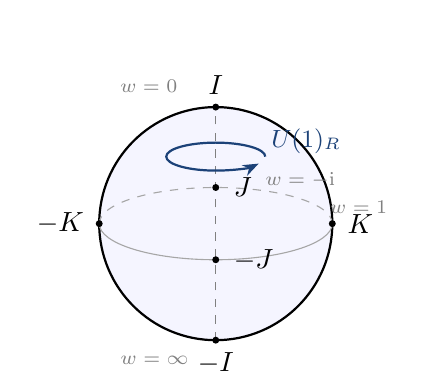
\begin{tikzpicture}[scale=0.74,>={Stealth[length=2mm]}]
  % 球面
  \fill[blue!4] (0,0) circle (2);
  \draw[thick] (0,0) circle (2);
  % 赤道：正面实线、背面虚线
  \draw[gray!70] (-2,0) arc (180:360:2 and 0.62);
  \draw[gray!70,dashed] (2,0) arc (0:180:2 and 0.62);
  % 南北轴
  \draw[gray,dashed] (0,-2)--(0,2);
  % 六个特殊点：w=0,∞ 在南北极；w=±i,±1 在赤道上
  \fill (0,2) circle (1.7pt) node[above=1pt] {$I$};
  \fill (0,-2) circle (1.7pt) node[below=1pt] {$-I$};
  \fill (2,0) circle (1.7pt) node[right=2pt] {$K$};
  \fill (-2,0) circle (1.7pt) node[left=2pt] {$-K$};
  \fill (0,0.62) circle (1.7pt) node[right=3pt] {$J$};
  \fill (0,-0.62) circle (1.7pt) node[right=3pt] {$-J$};
  % U(1) 轨道：绕 I 轴的小圆
  \draw[->,thick,kwblue] (0.85,1.15) arc (0:330:0.85 and 0.24);
  \node[kwblue,font=\small] at (1.55,1.42) {$U(1)_R$};
  % w 标注
  \node[gray,font=\scriptsize,align=left] at (-1.15,2.35) {$w=0$};
  \node[gray,font=\scriptsize,align=left] at (-1.05,-2.35) {$w=\infty$};
  \node[gray,font=\scriptsize] at (2.45,0.28) {$w=1$};
  \node[gray,font=\scriptsize] at (1.45,0.75) {$w=-\ii$};
\end{tikzpicture}
\caption{超凯勒流形的复结构族。球面是
$\{aI+bJ+cK\mid a^2+b^2+c^2=1\}\cong\PP^1_h$，三个正交的复结构 $I,J,K$ 是球面上
三个互相垂直的点；$U(1)_R$ 作用绕 $I$ 轴旋转，固定 $I$ 与 $-I$。按 \eqref{eq:Iw}，
$w=0,-\ii,1$ 分别给出 $I,J,K$。4d 族中「$\Psi=\infty$ 的 B-模型」落在 $J$（$w_+=w_-=-\ii$），
「$\Psi=0$ 的 A-模型」落在赤道大圆上的相反点对 $(w_+,w_-)=(-t,t^{-1})$，$t$ 实。}
\label{fig:hk-sphere}
\end{figure}

\subsubsection*{本节自检}
\begin{enumerate}
\item 为什么「$\MH$ 超凯勒」是 M2（S-对偶 $=$ 镜像对称）的必要条件？如果 $\MH$ 只有单个
复结构，S-对偶交换的是什么？
\item 用 \eqref{eq:Iw} 验证 $w=\ii$ 给出 $-J$、$w=-1$ 给出 $-K$。
\item $J^t\delta A_z=-\delta\varphi_{\bar z}$ 为什么等价于「$A+\ii\varphi$ 全纯」？
这个式子说明了 $J$ 与 $I$ 在对待 $C$ 的复结构上有什么不同？
\end{enumerate}

% ======================================================================
\subsection{$\MH$ 上的 Hitchin 纤维化：为什么它是可积系统（§4.3，pp.~50--56）}
\label{sec:fh-fib}

\subsubsection*{动机：把 $\MH$ 变成可计算的对象}

到 §\ref{sec:fh-hk} 为止，$\MH$ 只是一个「超凯勒商」：定义清楚，但不可计算。
它是非紧的、带奇点的、维数随 $g$ 增长的复流形；直接在上面做膜论或做 S-对偶，
无从下手。原文 §4.3 的任务是给 $\MH$ 一个\emph{可计算的结构}：一个到向量空间的
纤维化，其纤维是环面。这个结构同时是三个东西：
\begin{enumerate}
\item 一个\emph{代数完全可积系统}（Hitchin 1987）：基空间的线性函数就是互相对易的
  Hamiltonians，纤维是其等值面；
\item 一个\emph{特殊 Lagrangian 环面纤维化}：纤维在 $\omega_J,\omega_K$ 下是 Lagrangian，
  在复结构 $I$ 下是全纯子流形——这正是 SYZ 镜像对称所需的几何（§\ref{sec:fh-s}）；
\item 一个\emph{分级环的载体}：$\MH$ 在复结构 $I$ 下的全纯函数就是基 $B$ 上的全纯函数，
  因而 B-模型的 chiral ring 可以显式算出来（§\ref{sec:fh-s}）。
\end{enumerate}
第二、三条是本节全部技术工作的目的。原文在 §5.4 开头一句话点明：
「我们的目标是证明 S-对偶在 Hitchin 纤维化的基上经典地作用、在纤维上以 T-对偶作用」
（原句见 §\ref{sec:fh-s}）。没有 §4.3 的纤维化，这句话无法陈述。

\subsubsection*{构造：Casimir 不变量给出映射 $\pi:\MH\to B$}

设 $G$ 的秩为 $r$，$\mathfrak g$ 的基本不变多项式为 $P_1,\dots,P_r$，次数为
$d_1,\dots,d_r$（例如 $G=SU(N)$ 时 $d_i=i+1$，$i=1,\dots,N-1$）。Hitchin 映射定义为
\begin{equation}
\pi:\ \MH(G,C)\longrightarrow B:=\bigoplus_{i=1}^{r}H^0\bigl(C,K_C^{\,d_i}\bigr),
\qquad (E,\varphi)\longmapsto\bigl(P_1(\varphi),\dots,P_r(\varphi)\bigr).
\label{eq:hitchin-map}
\end{equation}
这里 $P_i(\varphi)$ 是把 $\varphi\in H^0(K_C\otimes\mathrm{ad}E)$ 代入不变多项式得到的
截面：$\varphi$ 的每个分量在 $K_C$ 中，$n$ 次多项式给 $K_C^{\,n}$ 中的截面。
在复结构 $I$ 下 $\pi$ 是全纯的；在复结构 $J$（平坦 $\gC$-丛）下 $\pi$ 有另一个解释
（monodromy 的特征值），但本节只用 $I$。\pA\anchor{src p.50}

维数计算是理解整个纤维化的关键，值得逐步写清。由 Riemann--Roch，
$\dim H^0(C,K_C^{\,n})=(2n-1)(g-1)$（$n\ge2$；基本不变量的次数 $d_i\ge2$，
所以 $n=1$ 的情形不会出现，无需担心 $K_C$ 的一次幂）。于是
\begin{equation}
\dim_\CC B=\sum_{i=1}^{r}(2d_i-1)(g-1)=(g-1)\sum_{i=1}^{r}(2d_i-1)=(g-1)\dim G ,
\label{eq:dimB}
\end{equation}
最后一步用了简单 Lie 代数的经典恒等式 $\sum_i(2d_i-1)=\dim\mathfrak g$。
而由 §\ref{sec:fh-hk}，$\dim_\CC\MH=2(g-1)\dim G$，所以
\begin{equation}
\dim_\CC B=\tfrac12\dim_\CC\MH .
\label{eq:halfdim}
\end{equation}
一个复维数一半的靶空间——这正是完全可积系统的维数特征。\pA\anchor{src p.50}

\subsubsection*{基的线性函数就是互相对易的 Hamiltonians}

原文给出 Hamiltonians 的显式形式：对每个不变多项式 $P$（次数 $n$）与
$\alpha\in H^1(C,K_C^{\,1-n})$，令\pA\anchor{src p.51}
\begin{equation}
H_{P,\alpha}=\int_C\alpha\,P(\varphi).
\label{eq:H}
\end{equation}
次数配平需要看清：$P(\varphi)$ 是 $K_C^{\,n}$ 的截面，而 $\alpha$ 按 Serre 对偶
是 $K_C^{\,1-n}$ 值的 $(0,1)$-形式；两者相乘得到 $(1,1)$-形式，才能在 $C$ 上积分。
而
\begin{equation}
\dim H^1\bigl(C,K_C^{\,1-n}\bigr)=\dim H^0\bigl(C,K_C^{\,n}\bigr)=(2n-1)(g-1),
\label{eq:serre}
\end{equation}
即 $\alpha$ 的空间恰是 $H^0(C,K_C^{\,n})^*$。换句话说，$H_{P,\alpha}$ 作为
$\bigl(P(\varphi)\bigr)$ 的线性函数，正是基 $B$ 上的一个\emph{线性坐标}。所以：
\begin{center}
\emph{基 $B$ 的线性函数 $\Longleftrightarrow$ 互相对易的 Hamiltonians。}
\end{center}
这解释了 \eqref{eq:halfdim} 的另一层含义：可积系统所需的 $\tfrac12\dim\MH$ 个独立
Hamiltonians，正好是 $B$ 的维数个线性函数。\pB\anchor{src p.51}

为什么它们互相对易？原文的论证分两步。第一步，在 $T^*\mathcal M\subset\MH$（$\varphi=0$
截面的余切方向的稠密开集，即「Hitchin 第二纤维化」给出的图卡）上，全纯辛形式是
$\Omega_I=\int_C\Tr\delta\varphi_z\wedge\delta A_z$，所以 $\varphi_z$ 与 $A_z$ 是共轭
变量。而 $H_{P,\alpha}$ 只依赖 $\varphi$（不依赖 $A$），因此任意两个这样的函数在
$\Omega_I$ 下的 Poisson 括号为零。第二步，Poisson 括号在超凯勒商下良定义
（商掉的是 Hamiltonian 作用），所以 $T^*\mathcal M$ 上的对易性延拓到整个 $\MH$。
原文把它总结为「$\MH$ 上存在 $\tfrac12\dim\MH$ 个对易的全纯函数，它们生成 $\MH$ 的
全纯函数环」。\pB\anchor{src p.52}

\subsubsection*{纤维：紧、全纯、Lagrangian、环面}

现在看映射 $\pi$ 的纤维 $\mathcal F_b=\pi^{-1}(b)$。原文给出的性质如下：\pA\anchor{src p.53}
\begin{itemize}
\item $\mathcal F_b$ 是紧复子流形（在复结构 $I$ 下全纯），复维数为
  $\dim_\CC\MH-\dim_\CC B=(g-1)\dim G$；
\item $\mathcal F_b$ 是复环面的 torsor（一个 torus 的平移），因此带交换群结构；
\item $\mathcal F_b$ 在 $\omega_J$ 与 $\omega_K$ 下是 Lagrangian 子流形
  （middle-dimensional，且两个辛形式在纤维上拉回为零）。
\end{itemize}
第三条是后文 SYZ 论证的关键。为什么会 Lagrangian？因为纤维由对易 Hamiltonians 的
等值面 $H_k=h_k$ 定义，是 middle-dimensional 的；而对易 Hamiltonians 的等值面在
Liouville--Arnold 意义下是 Lagrangian 的（原文 p.56 把这个推理一句带过，我们在这里
标为 \pB）。把它翻译成超凯勒语言就是：纤维在复结构 $I$ 下全纯（所以是复子流形），
又在 $\omega_J,\omega_K$ 下迷向（Lagrangian），这正是 SYZ 纤维化的要求。
\pB\anchor{src p.56}

\begin{keyidea}
\textbf{一句话记住 Hitchin 纤维化。}基 $B$ 是「可测量」的部分（Casimir 不变量，
经典可观测量的值），纤维 $\mathcal F_b$ 是「不可测量」的部分（环面，只能量子地感知）。
这句话在 §\ref{sec:fh-s} 会被原文用两个论证独立确认：chiral ring 论证（基上的全纯函数
就是全部局域算符）与 zerobrane 论证（点膜在纤维上移动，镜像是纤维上的 T-对偶）。
\end{keyidea}

\subsubsection*{附：Hitchin 第二纤维化与 $\mathcal M\hookrightarrow\MH$}

除了 $\pi:\MH\to B$，原文还用到第二个纤维化：忘掉 $\varphi$，把 $(E,\varphi)$ 送到
$E\in\MC$。它只在 $\varphi=0$ 附近定义良好，纤维是 $T^*\MC$ 的平移，而 $T^*\MC$ 是
$\MH$ 的稠密开集。两个纤维化横截：第一纤维化的纤维（环面）与第二纤维化的纤维
（仿射空间）互补。第二纤维化在推导 $B$-场的 $4\pi$ 系数与 §\ref{sec:fh-brane} 的
$(B,A,A)$-膜例子中都要用到；$\MC$ 在复结构 $I$ 下全纯、在 $\omega_J,\omega_K$ 下
Lagrangian，是「special Lagrangian」在超凯勒情形的类比物。\pA\anchor{src p.54}

\subsubsection*{图：纤维化与纤维-底空间}

\begin{figure}[htbp]
\centering
\begin{tikzpicture}[scale=0.72,>={Stealth[length=2mm]}]
  % 总空间外框
  \draw[fill=blue!3,draw=blue!45,rounded corners=7pt] (-4.3,0.60) rectangle (4.3,3.50);
  \node[font=\small,kwblue,anchor=west] at (-4.1,3.25) {$\MH$（复维 $2n$，超凯勒）};
  % 三根纤维（环面）
  \foreach \x/\h/\lab in {-2.7/1.50/{$b_1$}, 0/2.45/{$b_2$}, 2.7/1.15/{$b_3$}}{
    \draw[thick,fill=white] (\x,\h) ellipse (0.80 and 0.30);
    \draw[thick,fill=blue!8] (\x,\h) ellipse (0.27 and 0.10);
    \draw[gray,dashed] (\x,\h-0.30)--(\x,0.60);
    \fill (\x,0.60) circle (1.2pt);
    \node[above right=2pt,font=\small] at (\x,0.60) {\lab};
  }
  % 基空间
  \draw[thick] (-4.6,0.60)--(-0.8,0.60);
  \draw[thick] (0.8,0.60)--(4.6,0.60);
  \node[font=\small,anchor=north west] at (-4.6,0.40) {$B=\bigoplus_i H^0(C,K_C^{d_i})$};
  \node[font=\small,anchor=north east] at (4.6,0.40)
    {$\omega_J|_{\mathcal F}=\omega_K|_{\mathcal F}=0$};
  % pi 箭头
  \draw[->,thick] (3.72,1.00)--(3.72,0.64);
  \node[right,font=\small] at (3.72,0.82) {$\pi$};
\end{tikzpicture}
\caption{Hitchin 纤维化。基 $B$ 是复向量空间，复维 $(g-1)\dim G$；一般纤维
$\mathcal F_b$ 是复环面（画成环面），复维与基相同：$\dim_\CC\mathcal F=(g-1)\dim G$。
$\pi$ 对复结构 $I$ 全纯，纤维在 $\omega_J,\omega_K$ 下 Lagrangian；合起来即「特殊
Lagrangian 环面纤维化」，正是 SYZ 镜像对称要求的几何。}
\label{fig:hitchin-fibration}
\end{figure}

\subsubsection*{本节自检}
\begin{enumerate}
\item 为什么 $\dim_\CC B=\tfrac12\dim_\CC\MH$ 是「可积」的标志？如果基的维数不是一半，
换句话说什么会坏掉？
\item $H_{P,\alpha}$ 中 $\alpha\in H^1(C,K_C^{1-n})$ 的次数为什么必须是这样？如果取
$\alpha\in H^0$ 或 $H^1(C,\mathcal O)$，被积式还是 $(1,1)$-型吗？
\item 纤维的 Lagrangian 性用到了哪两个事实？为什么它对 SYZ 是必需的？
\end{enumerate}

% ======================================================================
\subsection{特殊化：$\Psi=\infty$ 给 B-模型、$\Psi=0$ 给 A-模型（§5.3，pp.~66--70）}
\label{sec:fh-spec}

\subsubsection*{动机：四维理论在二维里到底选了哪一对复结构}

§\ref{sec:fh-hk} 说明 $\MH$ 上有一整个 $\PP^1_h\times\PP^1_h$ 的参数族二维 TFT，由一对
复结构 $(J_+,J_-)$ 标记；而 §\ref{sec:fh-from4d} 只说「靶空间是 $\MH$」，没说四维理论
在二维极限里\emph{选了哪一点}。这一步不能省：M2 说「四维 S-对偶
$\tau\mapsto-1/\tau$ 在二维变成镜像对称」，而镜像对称的精确内容依赖 $(J_+,J_-)$。
本小节把这一点算出来。

\subsubsection*{$(J_+,J_-)$ 语言回顾}

把 $\MH$ 上的三个复结构统一记成 $I_w$（\eqref{eq:Iw}）。给定一对点
$(w_+,w_-)\in\PP^1_h\times\PP^1_h$，二维模型由无破缺超对称方程刻画：\pA\anchor{src p.59}
\begin{equation}
(1-\ii J_+)\,\partial\Phi=0,\qquad (1-\ii J_-)\,\bar\partial\Phi=0 ,
\label{eq:susy-pair}
\end{equation}
其中 $\partial,\bar\partial$ 是 $\Sigma$ 上的 $(1,0)$ 与 $(0,1)$ 部分，$J_\pm=I_{w_\pm}$
作用在拉回切丛上。两类特别情形是：
\begin{itemize}
\item $J_+=J_-=:J_b$（即 $w_+=w_-$）：两条方程合并为 $(1-\ii J_b)\dd\Phi=0$，
  在欧氏 $\Sigma$ 上迫使 $\dd\Phi=0$，即 $\Phi$ 常映射。称
  \term{B-model}{B-模型}（在复结构 $J_b$ 中）。
\item $J_-=-J_+$（即 $w_-=-1/w_+$，用 \eqref{eq:opposite}）：两条方程互为复共轭，
  任一都断言 $\Phi$ 在 $J_+$ 下全纯。称 \term{A-model}{A-模型}（准确地说，以
  $\omega_{J_+}$ 为辛形式的 A-模型）。
\end{itemize}
一般情形 $J_-\ne\pm J_+$ 下模型是广义 B-模型（原文 §5.2 用广义复几何约化为 A-模型，
本文件不展开）。于是判断「四维理论给了什么」就归结为计算 $(w_+,w_-)$。\pA\anchor{src p.59}

\subsubsection*{参数：$\tau$、$t$ 与 canonical parameter $\Psi$}

四维理论有两个参数：规范耦合 $\tau=\theta/2\pi+4\pi\ii/g^2$，以及扭化族参数 $t$
（来自 $(3.13)$，$t$ 实对应 $F'-t^{-1}D\varphi=0$ 的超对称条件）。二维模型却只依赖
一个组合的\emph{规范参数}：\pA\anchor{src p.66}
\begin{equation}
\Psi=\frac{\tau+\bar\tau}{2}+\frac{\tau-\bar\tau}{2}\cdot
\frac{t-t^{-1}}{t+t^{-1}} .
\label{eq:Psi}
\end{equation}
为什么？$t$ 与 $\tau$ 在二维模型中不独立：改变 $B$-场（由 $\operatorname{Re}\tau$ 给出）
与改变复结构（由 $t$ 给出）在广义复几何里是同一回事（原文 §5.2 的结论：$B$ 的
$(2,0)$ 分量与复结构空间中的移动等价）。$\Psi$ 就是 $\PP^1$ 上的坐标，把两种移动
合并成一个；模掉 $t\mapsto-t$ 与 $U(1)$ 作用后，理论只依赖 $\Psi$。
$\Psi$ 是这个族里的\term{canonical parameter}{规范参数}。\pA\anchor{src p.66}

\eqref{eq:Psi} 立刻给出两个特殊点：
\begin{itemize}
\item $t=\pm\ii$ 时 $(t-t^{-1})/(t+t^{-1})=\infty$，故 $\Psi=\infty$，\emph{与 $\tau$
  无关}（弱耦合极限也一样）；
\item $t=\pm1$ 时该因子为 $0$，故 $\Psi=\operatorname{Re}\tau$；特别地
  $\Psi=0$ 当且仅当 $t=\pm1$ 且 $\theta=0$（$\operatorname{Re}\tau=0$）。
\end{itemize}
这两个点正是 S-对偶（作为 $\Psi\mapsto-1/(n_g\Psi)$ 的分式线性变换）的不动点交换对。
$|t|=1$ 时 $\Psi$ 实；$|t|\ne1$ 时 $\Psi$ 可以取到整个上半或下半平面。\pA\anchor{src p.35}

\subsubsection*{$\Psi=\infty$：$J$ 中的 B-模型}

取 $t=\ii$。由 $(5.13)$，$w_+=-t=-\ii$，$w_-=t^{-1}=-\ii$，即
$(w_+,w_-)=(-\ii,-\ii)$。而由 \eqref{eq:Iw}，$w=-\ii$ 给出 $I_w=J$。因此在
$\Psi=\infty$ 处，二维模型是 $J$ 中的 B-模型：
\begin{equation}
\text{四维扭化理论}\big|_{\Psi=\infty}\ \cong\ B_J\bigl(\MH(G,C)\bigr).
\label{eq:BJ}
\end{equation}
原文的措辞是：「To get $\Psi=\infty$, we take $t=\ii$ and thus $(w_+,w_-)=(-\ii,-\ii)$.
The resulting model is the B-model in complex structure $J$.」\pA\anchor{src p.70}

物理上这很自然：$t=\pm\ii$ 是扭化族的「B-模型极限」，B-模型的无质量场是常映射，
对应四维理论里 $F'=0$ 的解在 $C$ 上的拉回；而 $J$ 正是使平坦 $G_{\CC}$-联络的复结构
（§\ref{sec:fh-hk}），常映射的靶空间点就是 $C$ 上平坦 $G_{\CC}$-丛。两者吻合。

\subsubsection*{$\Psi=0$：$K$ 中的 A-模型}

取 $t=1$（$t=-1$ 同理）。由 $(5.13)$，$w_+=-1$，$w_-=1$。注意
$w_-=-1/w_+$（因为 $-1/(-1)=1$），所以由 \eqref{eq:opposite}，
$I_{w_-}=-I_{w_+}$：这是一对相反复结构，模型是 A-模型。具体地 $w=\pm1$ 给出
$\pm K$，所以
\begin{equation}
\text{四维扭化理论}\big|_{\Psi=0}\ \cong\ A_K\bigl(\MH(G,C)\bigr).
\label{eq:AK}
\end{equation}
原文对 $t=0,\infty$ 的情形另有说明：那时得到 A-模型在 $\pm I$；而 $t=\pm1$ 给出
A-模型在 $\pm K$。这两族在 $S$-对偶下的行为不同，是 §\ref{sec:fh-s} 中 Table 2
的来源。\pA\anchor{src p.70}

\subsubsection*{S-对偶的作用：$B_J(G)\ \longrightarrow\ A_K(\Ldual)$}

现在到了本节的核心。$S$-对偶在四维是 $\tau\mapsto-1/(n_g\tau)$；在二维它必须同时
作用在 $t$ 上，因为扭化参数不是 S-对偶不变的（原文 (3.13)、(3.55)--(3.56)）：
\begin{equation}
S:\quad \tau\longmapsto-\frac{1}{n_g\tau},\qquad
t\longmapsto-t\,\frac{\tau}{|\tau|} .
\label{eq:S-on-t}
\end{equation}
在 $\PP^1_h$ 上，由 $(5.22)$，$S$ 作用为
\begin{equation}
w_+\longmapsto w_+\,\frac{c\tau+d}{|c\tau+d|},\qquad
w_-\longmapsto w_-\,\frac{|c\tau+d|}{c\tau+d},
\label{eq:S-on-w}
\end{equation}
其中 $S=\begin{pmatrix}a&b\\c&d\end{pmatrix}$。在 $\Psi$ 上，$(3.53)$--$(3.54)$ 给出
\begin{equation}
\Psi\longmapsto-\frac{1}{n_g\Psi} .
\label{eq:S-on-Psi}
\end{equation}
注意 \eqref{eq:S-on-Psi} 是分式线性变换，把 $\Psi=0$ 与 $\Psi=\infty$ 互换。

取最简单的例子：$\tau$ 纯虚（$\theta=0$），并取 $\Psi=\infty$ 的起点 $t=\ii$。
此时 $\tau/|\tau|=\ii$，所以
\begin{equation}
t'=-t\,\frac{\tau}{|\tau|}=-\ii\cdot\ii=1,\qquad\text{即}\qquad
(w_+,w_-)=(-t,t^{-1})\longmapsto(-1,1).
\label{eq:S-derivation}
\end{equation}
而 $(w_+,w_-)=(-1,1)$ 正是 $\Psi=0$ 的 A-模型在 $K$ 中。于是\pA\anchor{src p.70}
\begin{equation}
S:\qquad B_J\bigl(\MH(G,C)\bigr)\ \cong\ A_K\bigl(\MH(\Ldual,C)\bigr).
\label{eq:S-BtoA}
\end{equation}
这条式子是 M2 的第一次精确表述。它说的是：\emph{四维 S-对偶把 $J$ 中的 B-模型变成
$K$ 中的 A-模型}。注意两组复结构不同（$J$ 与 $K$）——这正是「镜像对称」的雏形：
两个理论在同一个（或对偶的）超凯勒流形上，却选择了不同的复结构。

\subsubsection*{从 $B_J\to A_K$ 到镜像对}

\eqref{eq:S-BtoA} 的左右两边复结构不同，还不是标准形式的镜像对称（标准形式要求
$B_J$ 与 $A_J$，即同一个复结构）。原文用一步补足：在 $S$ 之后再复合理论的自同构
\begin{equation}
\mathcal I:\ \varphi\longmapsto\ii\varphi ,
\label{eq:phi-i-phi}
\end{equation}
它把复结构 $K$ 旋转回 $J$（在 $\PP^1_h$ 上绕 $I$ 轴转 $90^\circ$）。这个自同构不是
四维族 $\PP^1_g$ 的对称（它把理论移出四维紧化族），但它保持二维模型的超对称代数
（作用在 $\varphi$ 的复结构上）。复合后得到
\begin{equation}
B_J\bigl(\MH(G,C)\bigr)\ \cong\ A_J\bigl(\MH(\Ldual,C)\bigr).
\label{eq:mirror-pair}
\end{equation}
原文的结论是：\pA\anchor{src p.70}
\begin{origquote}
“We get a mirror symmetry that maps the B-model in complex structure $J$ to the A-model in complex structure $J$. So $\MH(G,C)$ and $\MH({}^LG,C)$ are a mirror pair in complex structure $J$.”
\end{origquote}
当 $G=\Ldual$（例如 $G=G_2,F_4,E_8$，或自对偶的 $SU(N)$ 在特殊情形）时两个流形
是同一个，\eqref{eq:mirror-pair} 就是 $\MH$ 上\emph{到自身的}镜像对称。一般 $G$ 时
两个流形不同，但它们的 Hitchin 纤维化有相同的基（下一小节）。

\subsubsection*{Table 2：S-对偶在六个特殊点上的作用}

把上面两步合起来，就得到原文 Table 2（p.71）的内容。表中每一行是一个二维模型，
第二列是它在 S-对偶下的像：\pA\anchor{src p.71}
\begin{center}
\begin{tabular}{@{}ll@{}}
\toprule
起点 & 像 \\
\midrule
$I_B$ & $I_B$ \\
$I_A$ & $I_A$ \\
$J_B$ & $K_A$ \\
$J_A$ & $K_B$ \\
$K_B$ & $J_A$ \\
$K_A$ & $J_B$ \\
\bottomrule
\end{tabular}
\end{center}
注意 $I_B,I_A$ 是 S-对偶的\emph{不动点}：$I_w$ 在 $w=0$（$I$）与 $w=\infty$（$-I$）
处被 $U(1)_R$ 固定（§\ref{sec:fh-hk}），而 $S$ 作用在这个 $U(1)_R$ 上。所以
「$B$ 换成 $A$」只发生在 $J,K$ 那一对——$I$ 对 S-对偶是透明的。这解释了为什么
§5.4 的论证可以在 $I$ 里做（$I_B$ 不动），而结论却落在 $J_B$ 与 $K_A$ 上。
\pA\anchor{src p.71}

\begin{remark}[镜像对称的一个独立检验]
当 $G=\Ldual$ 时，任意把 $B_J$ 映到 $A_J$ 的镜像对称 $m$ 必保持上同调环的 cup
product（因 $\alpha\cdot\beta$ 与 $\alpha\cdot m^*\beta$ 都非零），却把 $(p,q)$ 型送到
$(n-q,n-p)$ 型（$n=\dim_\CC\MH$）。于是 B-模型的 $(p,q)$-算符数必须等于 A-模型的，
这是 \eqref{eq:mirror-pair} 非平凡的旁证。\pB\anchor{src p.71}
\end{remark}

\subsubsection*{图：$(\tau,\Psi)$ 平面与 S-对偶}

\begin{figure}[htbp]
\centering
\begin{tikzpicture}[scale=0.85,>={Stealth[length=2mm]}]
  % 左：τ 上半平面
  \begin{scope}
    \draw[thick] (-2.2,0)--(2.2,0);
    \node[below,font=\small] at (2.15,-0.02) {$\operatorname{Re}\tau$};
    \node[below left=0pt,font=\small] at (0,0) {$0$};
    \node[font=\small,align=center] at (1.35,1.52) {$\tau$ 上半平面};
    % 基本区域
    \fill[blue!8] (-0.5,0)--(0.5,0)--(0.5,1.4)--(-0.5,1.53)--(-0.5,0);
    \draw[blue!60] (-0.5,0)--(-0.5,1.53) (0.5,0)--(0.5,1.4);
    \draw[blue!60] (-0.5,1.53) arc (150:30:1.0 and 1.53);
    \fill (0,1.0) circle (1.2pt) node[right=2pt,font=\scriptsize] {$\ii$};
    % S 与 T
    \draw[->,thick,kwblue] (-1.75,0.25) to[bend left=25] node[above,font=\scriptsize] {$S$} (-0.25,1.75);
    \draw[->,thick,kwgreen] (1.85,0.35)--(0.85,0.35) node[midway,above,font=\scriptsize] {$T$};
  \end{scope}
  % 右：Ψ 球面
  \begin{scope}[xshift=6.2cm]
    \draw[thick] (0,0) circle (1.45);
    \draw[gray!70] (-1.45,0) arc (180:360:1.45 and 0.42);
    \draw[gray!70,dashed] (1.45,0) arc (0:180:1.45 and 0.42);
    \fill (0,1.45) circle (1.4pt) node[above=1pt,font=\small] {$\Psi=\infty$};
    \fill (0,-1.45) circle (1.4pt) node[below=1pt,font=\small] {$\Psi=0$};
    % 实轴
    \draw[gray,dashed] (-1.45,0)--(1.45,0);
    \node[font=\scriptsize] at (1.02,0.16) {$|t|=1$};
    \draw[->,thick,kwblue] (-0.75,1.05) to[bend right=40] node[above=1pt,font=\scriptsize] {$S$} (0.75,1.05);
    \node[font=\scriptsize] at (-0.75,0.52) {$|t|>1$};
    \node[font=\scriptsize] at (-0.75,-0.52) {$|t|<1$};
  \end{scope}
\end{tikzpicture}
\caption{左：$S$ 与 $T$ 在 $\tau$ 上半平面上的作用（基本区域用阴影画出，$S$ 把
$\tau=\ii$ 附近送向原点方向）。右：canonical parameter $\Psi\in\PP^1$。
$S$ 在 $\Psi$ 上是 $\Psi\mapsto-1/(n_g\Psi)$，把 $\Psi=0$（南极点，A-模型在 $K$ 中）
与 $\Psi=\infty$（北极点，B-模型在 $J$ 中）互换。赤道 $|t|=1$ 是 $\Psi$ 取实值的
轨迹（$\Psi=\operatorname{Re}\tau$）；上、下半球分别对应 $|t|>1$ 与 $|t|<1$。}
\label{fig:tau-psi}
\end{figure}

\paragraph{排除错误直觉之三：S-对偶不是把 $\Psi\to-1/\Psi$ 当作「另一个理论的参数」，
而是同一个二维理论族的坐标变换。}
$\Psi$ 是 $\PP^1$ 上的坐标，不是某个流形的模参数。S-对偶把 $\Psi$ 变成
$-1/(n_g\Psi)$，等价于把族中 $\Psi=0$ 的点与 $\Psi=\infty$ 的点对换——这正是
「B-模型与 A-模型互换」的精确含义。所以「四维 S-对偶在二维是镜像对称」不是一句
比喻，而是一个可计算的坐标变换。\pA\anchor{src p.67}

\subsubsection*{本节自检}
\begin{enumerate}
\item \eqref{eq:Psi} 中为什么 $\Psi$ 只依赖 $t$ 的比 $(t-t^{-1})/(t+t^{-1})$ 与 $\tau$？
如果 $t$ 与 $\tau$ 独立，二维模型会依赖两个参数，那会与 §\ref{sec:fh-from4d} 的哪个结论冲突？
\item 用 \eqref{eq:Iw} 验证 $w=-\ii$ 给 $J$、$w=\pm1$ 给 $\pm K$，从而核对
\eqref{eq:BJ} 与 \eqref{eq:AK}。
\item 为什么 $I_B,I_A$ 在 Table 2 中是 S-对偶的不动点？这与 §\ref{sec:fh-hk} 中
$U(1)_R$ 固定 $w=0,\infty$ 有什么关系？
\end{enumerate}

% ======================================================================
\subsection{S-对偶在 Hitchin 纤维化上的作用：基上经典、纤维上 T-对偶（§5.4--5.5，pp.~71--77）}
\label{sec:fh-s}

\subsubsection*{主命题}

上一小节给出了 M2 的\emph{代数}形式：$B_J(G)\cong A_J(\Ldual)$。但镜像对称是一个
关于\emph{范畴}的陈述（B-模型与 A-模型的 D-膜范畴等价），仅凭一个代数等式不足以
相信它。§5.4--5.5 给了两个独立的论证：一个用 B-模型的 chiral ring（基上），
一个用膜（纤维上）。合起来就是 SYZ 图像。原文把主命题写在 §5.4 开头：\pA\anchor{src p.71}
\begin{origquote}
“Our aim here and in section 5.5 is to show that S-duality acts classically on the base of the Hitchin fibration $\pi:\MH\to B$, while acting by T-duality on the fibers.” \anchor{src p.71}
\end{origquote}
这句话是全节的目标，也是本文件标题「S-对偶为什么就是镜像对称」的答案。

\subsubsection*{基上：chiral ring 论证}

先看基。B-模型在复结构 $I$ 中的 chiral ring 是
$H^q(X,\wedge^pT_X)$（双分次），其中 $p=q=0$ 的子环是 $X$ 上全纯函数的环。对
$X=\MH$ 在复结构 $I$ 下，这正是 $\MH$ 的全纯函数环。而 Hitchin 纤维化的纤维是
\emph{紧}复子流形（§\ref{sec:fh-fib}），所以 $\MH$ 上的全纯函数在每条纤维上为常数，
必是基 $B$ 上全纯函数的拉回：\pA\anchor{src p.72}
\begin{equation}
\Gamma\bigl(\MH,\mathcal O_{\MH}\bigr)\ \cong\ \Gamma\bigl(B,\mathcal O_B\bigr).
\label{eq:chiral-base}
\end{equation}
于是 B-模型的局域算符环只看见基 $B$，看不见纤维。若 S-对偶是 B-模型的范畴等价
（从 $G$ 到 $\Ldual$），则它诱导
\begin{equation}
\Gamma(B,\mathcal O_B)\ \cong\ \Gamma(\Ldual B,\mathcal O_{\Ldual B})
\label{eq:ring-iso}
\end{equation}
一个分次环同构。这就证明了「S-对偶在基上经典地作用」：它给出基之间的一个映射
$\Xi:B\to\Ldual B$。\pB\anchor{src p.72}

$\Xi$ 具体是什么？原文的论证走四维：四维理论的半 BPS 算符 $D_n$ 对应
$\mathrm{Sym}^n\mathbf 6$（$\mathbf 6=\wedge^2\mathbf 4$ 是 $SU(4)_R$ 的六维表示），
其最高权分量是 $G$-不变多项式 $P(\varphi)$。扭化后 $D_n$ 的共形维数为零、OPE 无奇异，
因此构成一个 $\CC^*$-分次环 $D'$。S-对偶把 $D_n(G)$ 送到 $D_n(\Ldual)$，故给出
$D'$ 的分次环同构；对单连通的 $G$ 这个作用是非平凡外自同构的补足（$G_2,F_4$ 上是
非平凡对合，一般 $G$ 由 $\Ldual$ 替换），在取好归一化后可以取为恒等。于是
$\Xi$ 由「$S$ 在基的生成元 $P_i(\varphi)$ 上作用」唯一确定：它是一个
\emph{仿射（线性）变换}，由 $\CC^*$ 的伸缩 $P_i\mapsto\lambda^{d_i}P_i$ 与
$\lambda\mapsto\lambda/\Psi$ 复合而成。\pB\anchor{src p.73}

基 $B$ 是向量空间，其坐标是 Casimir 不变量的值；S-对偶只能按次数重新标度它们
（$P_i$ 是 $d_i$ 次齐次），不能做非线性变换——否则会破坏 $B$ 的线性结构，而线性结构
正是 $U(1)$ 作用与可积系统 Hamiltonians 的来源。所以「基上的 S-对偶 $=$ 仿射变换
$\Xi$」不是假设，是 $B$ 的线性结构逼出来的。\pB\anchor{src p.73}

\subsubsection*{纤维上：为什么必须是 T-对偶}

基上没问题了，纤维上却出了麻烦。原文的原话是：\pA\anchor{src p.72}
\begin{origquote}
“there is no analogous way to show that S-duality acts classically on the fibers of the Hitchin fibration. It hardly can, given its relation to mirror symmetry!”
\end{origquote}
推理是：在 B-模型（复结构 $I$）里局域算符都是基上的全纯函数（\eqref{eq:chiral-base}），
它们测不到纤维上的位置；纤维上的动量对应 massive 态，而不是局域算符。所以 S-对偶
对纤维的作用\emph{不可能是经典映射}。而 SYZ 图像恰好要求：镜像对称在纤维上不是经典
映射，而是 T-对偶——在每一条环面纤维上取对偶环面。本情形下（\eqref{eq:ring-iso} 已
给出 $\Xi$）我们\emph{知道}基映射是什么，所以 SYZ 图像可以精确化：\pA\anchor{src p.77}
\begin{origquote}
“This is the usual SYZ picture of mirror symmetry, except that the map $\Xi$ is usually assumed to be trivial.” \anchor{src p.77}
\end{origquote}

\subsubsection*{膜论证：点膜在 S-对偶下的像必须支撑在对偶纤维上}

上面的论证是「不可能经典」，但还没证明「一定是 T-对偶」。§5.5 用零维膜把这个缺口
补上，这是本文最漂亮的一段推理，我们完整重建如下。\pA\anchor{src p.75}

\textbf{第一步：点 = $(B,B,B)$-膜。}$\MH$ 上的一个零维膜（点 $p$）没有标量场期望值，
其边界条件就是固定 $\Phi\equiv p$。点在任何复结构下都是复子流形（维数 $0$），配上
平凡线丛，所以它是 $(B,B,B)$-型的：相对于 $I,J,K$ 都是 B-膜。

\textbf{第二步：S-对偶后类型变成 $(B,A,A)$。}查 Table 2，$(B,B,B)\mapsto(B,A,A)$。
所以在对偶理论 $\MH(\Ldual)$ 中，像膜 $B_p$ 必须相对于 $I$ 是 B-膜、相对于
$J,K$ 是 A-膜。

\textbf{第三步：支撑维数两边夹。}A-膜在其辛形式下要求支撑至少是 middle-dimensional
（因为 A-模型需要 $2\,\Re\Omega$ 沿支撑非退化）；而 $B_p$ 的模空间（形变空间）只是
一个点，维数为 $0$，所以支撑至多 middle-dimensional。两边合并：$B_p$ 的支撑
\emph{恰好}是 middle-dimensional，即复维 $(g-1)\dim G$。

\textbf{第四步：中点就是纤维。}对于任意点 $q\in\MH(\Ldual)$，若 $q$ 在 $B_p$ 的支撑
上，则 $q$ 与 $p$ 有相同的 Casimir 不变量（因为 $p$ 是固定点，$B_p$ 只能沿基的
固定值移动），所以 $B_p$ 的支撑落在 $\Ldual\pi^{-1}(\Xi(\pi(p)))$ 内。两者都是
middle-dimensional，故支撑就是那条纤维。

\textbf{第五步：纤维上的平移。}点膜 $B_p$ 上的开弦无质量算符是 $\Phi$ 的取值函数；
而 $B_p$ 的支撑是纤维，$\Phi$ 在纤维上取遍所有值，所以 $B_p$ 的模空间就是纤维
$\mathcal F$ 本身。对偶膜 $\widehat B_p$ 的模空间则是「$\mathcal F$ 上的平坦
Chan-Paton 线丛」的模空间，即对偶环面 $\widehat{\mathcal F}$。于是 S-对偶给出
同构
\begin{equation}
\mathcal F\ \cong\ \widehat{\mathcal F}:=\operatorname{Hom}\bigl(\pi_1(\mathcal F),U(1)\bigr),
\label{eq:SYZ-fiber}
\end{equation}
即「纤维与对偶纤维是 T-对偶」。原文强调 rank $1$（不是更高 rank）：若取 rank $>1$
的 Chan-Paton 丛，$\widehat B_p$ 的模空间维数会大于 $B_p$，S-对偶就不可能是同构。
\pA\anchor{src p.76}

\begin{keyidea}
\textbf{整个论证链一句话。}点膜没有复结构可选（点在任何复结构下都全纯），故必为
$(B,B,B)$；S-对偶把它变成 $(B,A,A)$，而 $(B,A,A)$ 的 A-膜性质强迫其支撑为
middle-dimensional；于是像点「被迫」长大成一条纤维。这就是镜像对称把点送到环面的
机制，也是 SYZ 从四维理论里\emph{被推导出来}（而不是被假设）的原因。
\end{keyidea}

\subsubsection*{数学依据与微妙处}

原文指出 $\mathcal F\cong\widehat{\mathcal F}$ 在文献中已对若干情形独立知道：$G$ 为
酉群时由 Hausel--Thaddeus（[21]），$G=G_2$ 由 Hitchin（[81]），一般半单 $G$ 由
Donagi--Pantev（[82]）。本节不重新证明它们，只说明它们都是同一个四维 S-对偶的不同
侧面。微妙处：$G$ 的中心与基本群在 §7 才起作用（那时 $\Xi$ 不再是恒等）；$C$ 上的
spin 结构本文不分析。\pA\anchor{src p.77}


\paragraph{排除错误直觉之四：T-对偶发生在纤维上，不在底空间上。}
SYZ 镜像对称的 T-对偶作用在环面\emph{纤维}上，基 $B$ 上的映射 $\Xi$ 是经典的
（光滑甚至仿射的）。如果把 T-对偶理解成基上的变换，就会得到「镜像对称把 $B$ 映到
$B$ 之外」的错误结论。原文的措辞很明确：「S-duality acts classically on the base …
while acting by T-duality on the fibers」。基上可测（有局域算符），纤维上不可测
（无局域算符）——这两句话是同一件事。\pA\anchor{src p.71}

\paragraph{排除错误直觉之五：S-对偶在基上不是「把一个点送到另一个点」的任意映射。}
$\Xi$ 受两个约束：（i）它是分次环同构诱导的，因此保持基的线性结构（仿射）；（ii）
它把 $P_i$ 按次数 $d_i$ 标度，故与 $U(1)$ 作用相容。这两条使 $\Xi$ 不是任意的双射，
而是「$\CC^*$ 伸缩 + 可能的 $\Psi$ 依赖」的复合。相应地，S-对偶在 $\Psi$ 上的分式
线性作用 \eqref{eq:S-on-Psi} 不是 $\Xi$ 的作用，而是族参数的作用——两者不要混淆。
\pB\anchor{src p.73}

\subsubsection*{本节自检}
\begin{enumerate}
\item 为什么「局域算符测不到纤维」会迫使 S-对偶在纤维上取 T-对偶，而不是别的
  （例如恒等）？如果 S-对偶在纤维上取恒等，与 $\mathcal F\cong\widehat{\mathcal F}$
  矛盾在哪里？
\item 点膜论证的第三步用到了「A-膜支撑至少 middle-dimensional」与「点膜支撑至多
  middle-dimensional」。这两个「维数界」各自的来源是什么？
\end{enumerate}

% ======================================================================
\subsection{$\MH$ 上的膜分类与本文对镜像对称概念的贡献（§5.6，pp.~77--79）}
\label{sec:fh-brane}

\subsubsection*{类型 $(B,B,B)$、$(B,A,A)$、$(A,B,A)$、$(A,A,B)$}

$\MH$ 上有三个复结构 $I,J,K$，因此一张膜相对于每一个复结构都可以问「它是 A-型还是
B-型」。把三个答案写成三元组：$(B,B,B)$ 表示相对于 $I,J,K$ 都是 B-膜；$(B,A,A)$
表示对 $I$ 是 B-膜、对 $J,K$ 是 A-膜；等等。原文的清单是：\pA\anchor{src p.77}
\begin{itemize}
\item $(B,B,B)$：B-膜对每个复结构。点膜是例子；更一般地，space-filling 的
  全纯向量丛也给出这一类。
\item $(B,A,A)$：I-全纯的复子流形 $N$，且对全纯辛形式 $\Omega_I$ 是 Lagrangian 的
  （从而也对 $\omega_J,\omega_K$ Lagrangian）。例子：Hitchin 纤维
  $\mathcal F_b$；固定 $E$ 让 $\varphi$ 变化的 $T^*\mathcal M$ 纤维（此时
  $\Omega_I=\int\Tr\delta\varphi_z\wedge\delta A_z$ 在固定 $A$ 时为 $0$）。
\item $(A,B,A)$ 与 $(A,A,B)$：对 $J$（或 $K$）的复 Lagrangian 子流形。例子：固定
  $A_z=A_z+\ii\varphi_z$ 让 $A_{\bar z}$ 变化，即指定了全纯结构的平坦 $G_{\CC}$-丛。
\end{itemize}
注意 $(B,A,A)$ 的例子有一个统一的形式：$N$ 是复结构 $I$ 下的复子流形，且在
$\Omega_I$ 下 Lagrangian。这时它自动对 $\omega_J,\omega_K$ 也 Lagrangian
（因为 $\Omega_I=\omega_J+\ii\omega_K$ 在 $N$ 上为零意味着两个实部都为零）。
\pA\anchor{src p.78}

\subsubsection*{哪些类型不存在}

不是所有三元组都能实现。原文脚注 24 指出：\pA\anchor{src p.78}
\begin{origquote}
“there are no branes of type $(B,B,A)$: a subvariety holomorphic in complex structures $I$ and $J$ is automatically holomorphic in complex structure $K$.”
\end{origquote}
理由很干净：若 $N$ 同时是 $I$-全纯与 $J$-全纯的，由四元数关系 $K=IJ$，$N$ 自动
$K$-全纯；但「对 $K$ 是 A-膜」要求 $N$ 对 $\omega_K$ 迷向（Lagrangian），而一个
$K$-全纯子流形上 $\omega_K$ 的限制是 Kähler 形式，只有在 $N$ 为离散点时才为零——
所以非平凡的 $(B,B,A)$ 不存在。$(A,A,A)$ 同理：A-膜要求支撑 middle-dimensional，
三对相互矛盾的迷向性无法同时满足。\pB\anchor{src p.78}

\subsubsection*{S-对偶如何置换类型}

结合 Table 2，S-对偶对膜类型的作用是：\pA\anchor{src p.78}
\begin{equation}
(B,B,B)\longleftrightarrow(B,A,A),\qquad
(A,B,A)\longmapsto(A,B,A),\qquad
(A,A,B)\longmapsto(A,A,B).
\label{eq:brane-permutation}
\end{equation}
第一行正是点膜论证用的那一条：S-对偶把点膜变成支撑在纤维上的 $(B,A,A)$ 膜。第二、三行
说 $(A,B,A)$ 与 $(A,A,B)$ 是 S-对偶不变的\emph{类型}（具体的膜被送到另一张具体的膜，
类型不变）；这与 \eqref{eq:S-BtoA} 中 $J\leftrightarrow K$ 的交换一致——「B」所指的
复结构在两侧按 $\Xi$ 对应，故不冲突。\pB\anchor{src p.78}

\subsubsection*{本文对镜像对称概念的贡献}

现在可以回答本文件的中心问题：\emph{为什么说 S-对偶就是镜像对称？}

\textbf{第一，镜像对称在这里不是两个 Calabi--Yau 流形之间的等价。}标准表述是：
两个 CY 流形 $X,\hat X$ 的 A-模型与 B-模型等价。本文的情形不同：$X=\MH(G,C)$ 与
$\hat X=\MH(\Ldual,C)$ 是\emph{超凯勒}流形（非紧、带奇点），而且当 $G=\Ldual$
时它们\emph{是同一个流形}。镜像对称变成 $\MH$ 上两个不同复结构对应的 A/B 模型之间的
等价：$B_J\leftrightarrow A_J$（\eqref{eq:mirror-pair}）。所以它是\emph{同一个几何对象
上的两种量子场论}的等价，而不是两个几何对象之间的对应——这正是本文的贡献之一。
\pA\anchor{src p.70}

\textbf{第二，SYZ 纤维化是被推导出来的，不是被假设的。}标准 SYZ 假设镜像流形带特殊
Lagrangian 环面纤维化、且基上映射平凡。本文里 Hitchin 纤维化\emph{自动}提供这个结构
（§\ref{sec:fh-fib}），基映射 $\Xi$ 由 chiral ring 论证\emph{算出}
（\eqref{eq:ring-iso}），纤维上的 T-对偶由点膜论证\emph{证明}
（\eqref{eq:SYZ-fiber}）。原文说「except that the map $\Xi$ is usually assumed to be
trivial」（p.77），意思正是：一般 SYZ 中 $\Xi$ 平凡是假设，这里它由四维理论给出。
\pA\anchor{src p.77}

\textbf{第三，A/B 的「复结构选择」获得了四维解释。}在 $\MH$ 上选 $J$ 还是 $K$ 不是
任意的：$J$ 是 $\Psi=\infty$ 的 B-模型，$K$ 是 $\Psi=0$ 的 A-模型
（§\ref{sec:fh-spec}），而 S-对偶作用 $\Psi\mapsto-1/(n_g\Psi)$ 正好交换这两点。所以
「镜像对称交换 A 与 B」在四维就是一个关于 $\tau,t$ 的坐标变换——这是解释，不是类比。
\pA\anchor{src p.70}

\paragraph{排除错误直觉之六：B-模型不是「裸的拓扑 B-模型」的原样搬用。}
二维 B-模型的标准定义只需要靶空间是一个复流形；而在扭化理论里，B-模型还带着
B-场，B-场的 $(2,0)+(0,2)$ 分量与复结构一起构成\emph{广义复结构}（原文 §5.2）。
只有当 B-场取特殊值（或等价地，$\Psi$ 取特殊值）时，广义复结构才退化为普通复结构，
模型才是「纯」B-模型。所以「$\MH$ 上的 B-模型」有两层意思：（i）复结构 $I$（或 $J$）
中的纯 B-模型；（ii）带 B-场的广义 B-模型。§5.3 的特殊化 $\Psi=\infty$ 与 $\Psi=0$
正是从（ii）退化到（i）的两个点。混淆这两层会把 Table 2 读错。\pB\anchor{src p.69}

\paragraph{排除错误直觉之七：镜像对称不是「两个 CY 流形之间的等价」这么简单。}
如第一点所述，本情形中两个流形可以相同（$G=\Ldual$），镜像对称是同一个流形上
不同复结构对应的模型之间的等价；更准确地说，它是\emph{二维 TFT 族}（由 $(J_+,J_-)$
标记）内部的一个对称性，而四维 S-对偶是这个族上的一个具体变换；读成「$X$ 与
$\hat X$ 的对应」会漏掉「同一流形、不同复结构」这一层。\pA\anchor{src p.77}

\subsubsection*{本节自检}
\begin{enumerate}
\item 为什么 $(B,A,A)$ 膜的支撑自动对 $\omega_J,\omega_K$ Lagrangian？用
  $\Omega_I=\omega_J+\ii\omega_K$ 写出来。
\item 脚注 24 的论证里，哪一步用到了「$K=IJ$」？如果 $I,J,K$ 不满足四元数关系，
  结论会怎样？
\item 本文说「SYZ 在这里是定理而不是假设」，具体指哪两个论证？它们各自证明了什么？
\end{enumerate}

% ======================================================================
\subsection*{本文件在全书中的位置}
\noindent\textbf{S3}（\S\ref{sec:fh-from4d}--\ref{sec:fh-fib}）：四维理论在 $\Sigma\times C$ 上紧化，靶空间 $\MH$；$\MH$ 是超凯勒商、带 $\PP^1_h$ 族复结构与 Hitchin 纤维化，产出「$\MH$ 上的二维 TFT 族」。\textbf{S4}（\S\ref{sec:fh-spec}--\ref{sec:fh-brane}）：$\Psi=\infty$ 给 $B_J$、$\Psi=0$ 给 $A_K$，S-对偶交换它们，即 $B_J(G)\cong A_J(\Ldual)$（这就是 M2），产出「$\MH$ 上的 A/B 模型范畴及其等价」。\textbf{S5 之后}：线算子作为 $\MH$ 上的膜算子来读，类型正是 \S\ref{sec:fh-brane} 的 $(B,A,A)$ 等；eigenbrane 是 Hitchin 纤维上的 $(B,A,A)$ 膜，Hecke 特征层由固定 $A_z$ 的 $(A,B,A)$ 膜构造，D-模的配对落到 \S\ref{sec:fh-s} 的 SYZ 对偶上——没有 \S\ref{sec:fh-hk} 的三复结构与 \S\ref{sec:fh-fib} 的纤维化，这些步骤都无法陈述。

若只想记住一件事：\emph{$\MH$ 上的镜像对称 $=$ 同一个超凯勒流形上 $J$ 与 $K$ 两个复结构之间的 A/B 交换 $=$ 四维 S-对偶在二维的像}；而这一切之所以可能，是因为 $\MH$ 是超凯勒的，而它超凯勒是因为它是四维 Hitchin 方程解的超凯勒商。

% ======================================================================
%  32_flesh_hecke.tex
%  骨血层之三：'t Hooft 算子 = 几何 Hecke 算子
%  主链 S7；节点 N9（§9）、N10（§10）；miracle M3
%  底本：§6.2（印刷 pp.81–89 → p082–p090）、§9（pp.123–147）、§10（pp.148–183）
%  只写本文件；不改 preamble / main / 他人文件
% ======================================================================

\section{骨血层之三：\texorpdfstring{'t Hooft}{'t Hooft} 算子就是几何 Hecke 算子}
\label{sec:flesh-hecke}

\begin{kcard}{本节的位置：主链 S7，节点 N9--N10，miracle M3}
\anchor{§9 开篇 p.123；§10 开篇 p.148；§6.2 p.81}
\textbf{一句话。}在拓扑扭化参数取 $\Psi=0$（$t=1$、$\theta=0$）时，把 $\mathcal{N}=4$ 超对称
Yang--Mills 理论紧化到 $M=\RR\times I\times C$，在 $W=I\times C$ 中一点 $p$ 处插入静态
't Hooft{} 算子 $T(\Ldual R)$。越过 $p$ 所在的时间切片 $y=y_0$ 时，膜上的全纯 $G$-丛
$E_y\to C$ 经历的跳变，\emph{恰好}是型 $\Ldual R$ 的 Hecke 修改。这就是 \textbf{S7}，
其内容一句话概括为 \textbf{M3}：“'t Hooft{} 算子作用在规范丛上的效果恰好是
Hecke 修改”。\pA\anchor{src p.127}

\textbf{本节的输入与输出。}
输入是 S5（线算子 $=$ 膜算子，§6）与 S4（$\MH$ 上的膜范畴，§5）；
输出是 S8（§11--§12 用典范余各向同性 A-膜把 Hecke 算子翻译成 $\Dmod$-模）所必需的
\emph{算子侧}词典：膜上的算子不是抽象代数生成元，而是 “几何对象的局部修改”。\pB\anchor{§8 的入口}

\textbf{为什么这段最难。}因为它把三种互不相同的对偶叠在同一处：
S-对偶（$\tau\mapsto-1/\tau$，交换 Wilson 与 't Hooft）、
GNO 对偶（$G\leftrightarrow\Ldual G$，表示 $\leftrightarrow$ 余权）、
几何 Langlands 对偶（$\MH(G)$ 的 A-膜 $\leftrightarrow$ $\MH(\Ldual G)$ 的 B-膜）。
读者最常见的失败模式，是把 \textbf{M3} 当成前两种对偶中某一种的直接推论；它不是，
它是第三种对偶在\emph{算子}层面的表现。这一点我们在 §\ref{sec:flesh-hecke-claim} 用一整段澄清。
\end{kcard}

\subsection*{符号约定}

本文件沿用 \texttt{02\_符号与风格卡} 的固定符号（$G$、$\Ldual$、$\gC$、$C$、$g$、$\MH$、$\tau$、
$t$、$\Psi$、$\phi$、$A$、$F$、$E$、$Q$、$Z(B)$ 等），只新增下表所列者。凡新增符号在
首次出现处重复一次定义；引用骨架节点一律写 $S7$、$N9$、$M3$ 这样的形式。

\begin{center}\small
\begin{tabular}{@{}lll@{}}
\toprule
\tabhead{符号} & \tabhead{含义} & \tabhead{出处}\\
\midrule
$x$，$p_0$ & $C$ 上的插入点（$C$ 为紧 Riemann 面，亏格 $g$） & \anchor{src p.128}\\
$W=I\times C$ & 三维流形；$I$ 为区间，$C$ 为 Riemann 面 & \anchor{src p.149}\\
$y$ & $I$ 的坐标；$E_y=E|_{\{y\}\times C}$ & \anchor{src p.129}\\
$\mathcal{O}(x)$ & $C$ 上在 $x$ 外全纯、至多 $x$ 处单极点的函数对应线丛 & \anchor{src p.130}\\
$\mathcal{Y}(\Ldual R)$，$\mathcal{Y}(\Ldual w;x)$ & 型 $\Ldual R$（或最高权 $\Ldual w$）的 Hecke 修改空间 & \anchor{src p.137}\\
$\mathrm{Gr}_G$ & 仿射 Grassmann 流形 $G_{\CC}((z))/G_{\CC}[[z]]$ & \anchor{src p.146}\\
$\mathcal{Z}(\Ldual w_1,p_1;\dots)$ & 带指定奇异性 Bogomolny 方程解的模空间 & \anchor{src p.156}\\
$\mathrm{IH}^\bullet$ & 交集上同调 & \anchor{src p.174}\\
$K$ & A-模型的幽灵数（ghost number） & \anchor{src p.173}\\
$N_\alpha$ & 张量积重数空间 $\mathrm{Hom}_{\Ldual G}(\Ldual R\otimes\Ldual R',\Ldual R_\alpha)$ & \anchor{src p.167}\\
$\mathcal{Q}$ & Higgs 丛的 Hecke 对应（不用 $Q$，避免与超荷冲突） & \anchor{src p.182}\\
$\rho$ & 同态 $U(1)\to G$；其共轭类即 GNO 荷 & \anchor{src p.84}\\
$\Ldual w=(m_1,\dots,m_N)$ & $\Ldual G$ 的最高权（对 $G=U(N)$ 为整数 $N$-plet） & \anchor{src p.131}\\
$\Delta$ & 修改空间的复维数 & \anchor{src p.144}\\
\bottomrule
\end{tabular}
\end{center}

\subsection{导言：三层任务与一条主线}\label{sec:flesh-hecke-intro}

这一段（原文 §6.2、§9、§10）要建立的东西可以拆成三层，而这三层在原文里是
\emph{交织}着写的：§6.2 给物理定义，§9 给数学对象并直接宣布二者相等，
§10 才回过头用 Bogomolny 方程把“相等”变成模空间的相等。我们的任务是把它拆开、
把被跳过的步骤补上、并标出哪些地方原文实际上是“用物理论证代替了证明”。

\begin{keyidea}
\textbf{三层任务。}
\begin{enumerate}
\item \textbf{物理层}（§6.2）：'t Hooft{} 算子是\emph{无序算子}（disorder operator），
  它不测量场的某个值，而是规定场沿一条线的奇异性；插入了它的路径积分，是在
  \emph{带奇异性}的场上做的。\pA\anchor{src p.81}
\item \textbf{数学层}（Beilinson--Drinfeld）：Hecke 修改是把 $C$ 上一点 $x$ 处的
  $G$-丛 $E$ 换成 $E'$，使 $E'$ 与 $E$ 在 $C\setminus\{x\}$ 上同构，而 $x$ 处的
  “差”由一个仿射 Grassmann 流形的 Schubert 胞腔的参数刻画。\pA\anchor{src p.146}
\item \textbf{相等}（§9.1、§10.3）：4d 理论紧化到 2d 后，'t Hooft{} 算子对膜上的
  全纯丛的作用，就是第二层的 Hecke 修改；并且这个相等可以被提升为
  \emph{模空间的相等}：Bogomolny 方程解空间（带边界条件）$\mathcal{Z}$ 与
  修改空间 $\mathcal{Y}$ 是同一个复流形。\pA\anchor{src p.162}
\end{enumerate}
\end{keyidea}

\textbf{为什么必须拆成三层。}
如果只读 §9.1，读者会觉得 \textbf{M3} 是一个\emph{奇迹}：物理上插入一根奇异的线，数学上丛就
被修改了。但 \textbf{M3} 不是奇迹，它是\emph{可以逐条验证}的：'t Hooft{} 算子的奇异数据是一个
同态 $\rho:U(1)\to G$；Hecke 修改的类型是仿射 Grassmann 中一个 $G_{\CC}([[z]])$-轨道；
而这两者是\emph{同一个} $\rho$（其一为实数形式，另一为其复化）。这个“同一个 $\rho$”
就是全篇的枢纽，我们在 §\ref{sec:flesh-hecke-gr} 把它写成一条显式的等式。\pB\anchor{src p.147}

\textbf{一条主线（建议读者按此顺序读）。}
\begin{enumerate}
\item §\ref{sec:flesh-hecke-thooft}：先弄清 't Hooft{} 算子是什么，尤其是它\emph{为什么不是}
  一个通常意义上的算子（这一点原文 p.123 说得很明确，却常被忽略）。
\item §\ref{sec:flesh-hecke-hecke}：Hecke 修改的定义与两个最小例子
  （$G=GL_1$、$G=GL_2$），以及在什么意义上它是“局部”的。
\item §\ref{sec:flesh-hecke-claim}：把 §9.1 的论证链逐条重建成七个命题，
  各标 $A$/$B$，得到 M3 的确切陈述。
\item §\ref{sec:flesh-hecke-gr}：仿射 Grassmann 与 Schubert 分层，说明修改类型的
  参数空间是什么。
\item §\ref{sec:flesh-hecke-s10}：§10 的四件技术工作（边界条件、单极子冒泡、
  Kähler 商、OPE 与扩展 Bogomolny 方程），以及
\item §\ref{sec:flesh-hecke-honest}：怎样诚实地读这一段——哪些是定理，哪些是物理论证。
\end{enumerate}

\textbf{五个最容易犯的错。}（'t Hooft{} 不是 Wilson 的对偶那么简单；Hecke 不是换掉丛；
不是所有修改都等于张量 $\mathcal{O}(x)$；“算子”不按字面读；M3 不是前两种对偶的推论。）
这里不展开——后文给了五张“排除错误直觉”卡片，逐条对照即可。


\subsection{第一层：\texorpdfstring{'t Hooft}{'t Hooft} 算子的物理定义（§6.2，pp.~81--89）}
\label{sec:flesh-hecke-thooft}

\subsubsection{动机：为什么必须发明一种新的算子}

在 $\Psi=\infty$（$t=\pm\ii$）的拓扑扭化理论里，Wilson 算子是现成的：取 $G$ 的一个表示 $R$、
一条闭曲线 $S$，算 Wilson 算子就是算 $S$ 上联络的和乐（holonomy）在 $R$ 中的迹。它是
\term{order operator}{有序算子}：先有一个经典表达式（和乐），再把它当量子算子用。\pA\anchor{src p.81}

但 S-对偶要求有对偶对象。对偶变换 $S:\Psi\mapsto-1/n_g\Psi$ 把 $\Psi=\infty$ 送到
$\Psi=0$；于是“$\Psi=0$ 处的理论里的某个算子”应当与 Wilson 对偶。问题在于：
$\Psi=0$ 时理论里没有任何现成的和乐型表达式可用——扭化参数取这个值时，被保留的
超荷是另一个，能写成经典表达式的量变了。\pA\anchor{src p.81}

出路是\emph{反过来}定义算子：不规定“沿 $S$ 的和乐等于什么”，而规定
“场在 $S$ 附近必须怎样奇异”。这就是 \term{disorder operator}{无序算子}：
它的定义不是作用的表达式，而是路径积分的一个\emph{约束}（边界条件）；
然后\emph{在满足该奇异性的场空间中}做路径积分。原文的原话是：无序算子的定义方式
是“规定经典场应当具有的奇异性，并在奇异性存在的情况下做路径积分”。
\pA\anchor{src p.81}

\begin{keyidea}
\textbf{两类算子的对偶是“同一件事的两种描述”，不是“两个算子相乘”。}
在量子力学里，有序算子与无序算子可以在适当情形下有相同的代数性质，并且常常在对偶下
互换。Wilson 的对偶（在 $\Psi=0$ 的理论里）就是 't Hooft{} 算子。
这句话的\emph{内容}是：$\Psi=\infty$ 一侧的表示论数据（$G$ 的表示 $R$）
与 $\Psi=0$ 一侧的表示论数据（$\Ldual G$ 的表示 $\Ldual R$）互为对偶，
不是“同一个算子的两个名字”。\pA\anchor{src p.81}
\end{keyidea}

这里有一个容易被忽略的技术细节，它在本节的公式里反复出现：定义 Wilson 算子需要
曲线 $S$ 的\emph{定向}；而定义 't Hooft{} 算子需要 $S$ 的\emph{法丛}的定向。
把 $S$ 的小邻域等同于 $S\times\RR^3$、记 $\epsilon_3$ 为 $\RR^3$ 的体积形式、$r$ 为到
$S$ 的距离，则
\begin{equation}
\epsilon_3=\dd r\,\dd\mathrm{Vol},
\label{eq:eps3}
\end{equation}
't Hooft{} 算子的定义只依赖法丛的定向。\pA\anchor{src p.81}\anchor{eq 6.6}

\subsubsection{最小例子：$G=U(1)$ 与奇异 Dirac 单极子}

先看最简单的：\term{Dirac monopole}{Dirac 单极子}。$\RR^4=\RR\times\RR^3$，坐标
$(s,\vec x)$，奇异沿直线 $L=\{\vec x=0\}$。$\mathrm{U}(1)$ 的 Maxwell 方程是
$\dd F=\dd\star F=0$，它在 $\RR^3\setminus\{0\}$ 上有旋转与平移对称的解
\begin{equation}
F=\frac{\ii}{2}\star\dd\frac{1}{|\vec x|}.
\label{eq:dirac}
\end{equation}
（$\star$ 表明这个解依赖法丛的定向。）把它沿 $s$ 方向拉回到 $\RR^4\setminus L$ 即可。
归一化选得使包围奇点的 $S^2$ 上
\begin{equation}
\oint\frac{\ii F}{2\pi}=1
\qquad\Longleftrightarrow\qquad
\oint_{Y}c_1(L)=1,
\label{eq:flux1}
\end{equation}
即存在一个曲率为 $F$ 的酉线丛 $L\to\RR^4\setminus L$，其第一陈数在包围奇点的球面上为 $1$。\pA\anchor{src p.83}
\anchor{eq 6.7}

于是 $G=U(1)$ 的基本 't Hooft{} 算子 $T(0)$ 定义为：\emph{在 $M\setminus S$ 上对
abelian 规范场做路径积分，并要求靠近 $S$ 时场与奇异 Dirac 单极子一致}；
等价的微分条件是 $F$ 在 $S$ 附近发散为
\begin{equation}
F\sim\frac{\ii}{2}\star_3\dd\frac{1}{r},
\label{eq:sing}
\end{equation}
其中 $\star_3$ 是法向平面上的 Hodge 星。更一般地取整数 $m$，要求奇异部分为
$(\ii m/2)\star_3\dd(1/r)$，就得到磁荷 $m$ 的算子 $T(m)$。\pA\anchor{src p.82}
\anchor{src p.83}

这里已经埋下了本节最重要的伏笔：'t Hooft{} 算子的\emph{全部}内容就是
“把路径积分的定义域从\{全体场\}限制到\{在 $S$ 附近有指定奇异性的场\}”。
它没有“作用在态上”的公式，而是一个\emph{几何约束}。后面我们会看到，
在紧化到二维之后，这个几何约束恰好可以用“丛的局部修改”来翻译。

原文还补了一句拓扑上的警告：若 $S$ 的同调类在 $H_1(M,\ZZ)$ 中非零，则 $\mathrm{U}(1)$
理论里根本不存在这样的规范场，路径积分取零；对偶地，Wilson 算子的期望值也为零。
这说明 't Hooft{} 算子的“定义域”本身就带着拓扑信息。\pA\anchor{src p.82}

\subsubsection{拓扑对称要求奇异的是整个超多重态，不只是规范场}

上面的定义只规定了 $F$ 的奇异性。但 $\Psi=0$ 处我们要求算子保持\emph{拓扑对称}
（即扭化后保留下来的那个标量超荷）。判据是：'t Hooft{} 算子保持拓扑对称，当且仅当
场在 $S$ 附近的奇异行为与拓扑对称相容。对 abelian 情形取 $t=1$、$\tau$ 虚，
保持拓扑对称的场条件是
\begin{equation}
(F+\dd\phi)_+=(F-\dd\phi)_-=0,
\label{eq:topysym}
\end{equation}
而若 $F$ 有 Dirac 奇异、$\phi$ 光滑，这个条件不满足。\pA\anchor{src p.83}\anchor{eq 6.8}

因此 $\phi$ 也必须奇异。取 $s$ 为沿 $L$ 的“时间”坐标，
\begin{equation}
F=\frac{\ii}{2}\star_3\dd\frac{1}{|\vec x|},
\qquad
\phi=\frac{\ii}{2|\vec x|}\,\dd s,
\label{eq:phising}
\end{equation}
则 \eqref{eq:topysym} 被满足。\pA\anchor{src p.83}\anchor{eq 6.9}

这一步是很多读者会漏掉的：'t Hooft{} 算子不是“只对规范场设条件”，
它必须把 Higgs 场（或者说 $\phi$ 的相应分量）也一起做成奇异的，否则它破坏拓扑对称、
在拓扑理论里根本不合法。这个“$\phi$ 也要奇异”的事实，正是 §\ref{sec:flesh-hecke-s10}
里扩展 Bogomolny 方程（$\phi$ 有全纯截面结构）的物理起源。\pB\anchor{src p.83}

\subsubsection{一般 $G$：同态 $\rho:U(1)\to G$ 与 GNO 荷}

推广到任意紧致李群 $G$：取任意同态 $\rho:U(1)\to G$，要求场沿 $S$ 的奇异性是
\eqref{eq:phising} 在 $\rho$ 下的像。算子只依赖 $\rho$ 的共轭类。\pA\anchor{src p.84}

关键的表示论事实是：$\rho$ 的共轭类由 $\Ldual G$ 的最高权分类，也就是由 $\Ldual G$
的不可约表示分类。因此对每个不可约表示 $\Ldual R$ 与每条一维曲线 $S$，有一个拓扑
't Hooft{} 算子 $T(\Ldual R,S)$，简写 $T(\Ldual R)$。\pA\anchor{src p.84}

原文把这句话称为“经典 GNO 对偶”（Goddard--Nuyts--Olive），并指出参考文献
[90] 的贡献在于把它\emph{重述为算子}而不是态：GNO 原本分类的是磁单极子的荷，
而这里同一个组合数据被用来定义一类线算子。\pA\anchor{src p.84}

对 $G=U(N)$，同态 $\rho$ 可以取成
\begin{equation}
\rho(\ee^{\ii\alpha})=\mathrm{diag}\bigl(\ee^{\ii m_1\alpha},\dots,\ee^{\ii m_N\alpha}\bigr),
\qquad m_1\ge m_2\ge\cdots\ge m_N,
\label{eq:rhoUN}
\end{equation}
于是 't Hooft{} 算子由整数 $N$-plet $\Ldual w=(m_1,\dots,m_N)$（模置换）刻画；
在 Lie 代数层面 $\rho$ 把 $1\in\mathfrak{u}(1)$ 送到 $\mathrm{diag}(m_1,\dots,m_N)$。\pA\anchor{src p.131}
\anchor{eq 9.11}
相应地，算子 $T(\Ldual w)$ 的奇异条件是：$p$ 附近曲率的奇异部分为
\begin{equation}
F\sim\frac{\ii}{2}\star\dd\frac{1}{|\vec x-p|}\cdot\mathrm{diag}(m_1,\dots,m_N).
\label{eq:Fdiag}
\end{equation}
\pA\anchor{src p.132}\anchor{eq 9.12}

\subsubsection{IR 拓扑版本为什么可以被理解为“对规范丛的修改”}

这是任务要求的第一问，也是本小节最需要重建的一步。原文在 p.84 只用了一句话把它带过：
't Hooft{} 算子的分类“与 Grothendieck 的 $\mathbb{P}^1$ 上 $G$-丛分类密切相关”。
我们把它展开成三步。

\begin{keyidea}
\textbf{三步论证。}
(i) 把 $S^2$ 等同于包围奇异点的球面：构造 $T(\Ldual R)$ 用的 abelian 解在 $S^2$ 上给出
一个 $G$-丛，而 $\mathbb{P}^1$ 上全纯 $G$-丛正由 $\mathcal{O}(1)$ 经 $\rho:U(1)\to G$
（复化后 $\rho_{\CC}:\CC^*\to G_{\CC}$）给出。\pA\anchor{src p.84}
(ii) 反向也成立：$\mathbb{P}^1$ 上每个 $G$-丛（即使不稳定）都有 Yang--Mills 联络，
而每个 YM 解都等价于构造 't Hooft{} 算子用的 abelian 解。\pA\anchor{src p.84}
(iii) 故 't Hooft{} 算子的分类 $=$ $\mathbb{P}^1$ 上 $G$-丛的分类；同一句话在四维是
“在 $S$ 附近保留一个指定的丛”，在二维是“在点 $x$ 处保留一个指定的丛”。
\pA\anchor{src p.84}
\end{keyidea}

第三步的“二维表述”是本文的关键：一旦理论紧化到 $C$ 上（$M=\RR\times I\times C$），
包围奇异线的球面 $S^2$ 就被换成了 $C$ 上包围点 $x$ 的\emph{小圆盘}。于是
“$\Psi=0$ 时保持拓扑对称的 't Hooft{} 算子”在二维图像里就是：
“在 $x$ 的小圆盘上换一个丛，圆盘外不动”。这正是 Hecke 修改的定义。
这个翻译是 $B$ 级重建：原文没有把它写成一句命题，但 p.84 的“分类相同”加上
§9.1 的具体计算足以支撑它。\pB\anchor{src p.84；重建依据：p.132 的 $\oplus L_i$ 分解与 p.146 的
仿射 Grassmann 表述}

还有一个拓扑细节值得单独记下：$\mathbb{P}^1$ 上的全纯 $G$-丛可以拓扑非平凡。
$G$-丛的拓扑由 $\xi\in H^2(S^2,\pi_1(G))\cong\pi_1(G)$ 分类，而
$\pi_1(G)\cong Z(\Ldual G)$；构造 $T(\Ldual R)$ 所用的球面上的丛非平凡，
当且仅当 $\Ldual G$ 的中心在 $\Ldual R$ 上非平凡作用。\pA\anchor{src p.84}
用 \eqref{eq:rhoUN} 的语言说：$\sum_i m_i\ne 0$ 时 $T(\Ldual w)$ 会改变 $G$-丛的拓扑
（因为 $c_1\mapsto c_1+\sum_i m_i$，见 \eqref{eq:c1shift}）；$\sum_i m_i=0$ 时拓扑不变。
这个判据在 §\ref{sec:flesh-hecke-claim} 会以“分解后每根线丛各自被张量化”的形式
再次出现。\pB\anchor{src p.133}

\begin{kcard}{排除错误直觉 1：“'t Hooft{} 算子就是 Wilson 算子的对偶”这句话不能这样用}
\anchor{src p.81；src p.87}
\textbf{错误理解：}既然 S-对偶交换 $\Psi=\infty$ 与 $\Psi=0$，那么把 Wilson 算子
（和乐的迹）换成“对偶表示的和乐”就得到 't Hooft{} 算子。

\textbf{为什么错：}
(i) 't Hooft{} 算子的定义不是任何经典量的量子化，而是路径积分的\emph{定义域约束}；
在 $\Psi=0$ 的理论里没有“和乐型”的表达式可以替换。\pA\anchor{src p.81}
(ii) 只有\emph{有理} $\Psi$ 时才能把 Wilson 与 't Hooft{} 拼成一个保持拓扑对称的
复合算子 $WT_{n,m}$；一般 $\Psi$ 下 't Hooft{} 算子破坏拓扑对称，需要乘一个
Wilson 因子才能修复，而规范不变性又要求 $n=-m\Psi$ 为整数。所以
“纯 't Hooft{} 算子”只在 $\Psi=0$ 这一个点上作为拓扑算子存在。\pA\anchor{src p.87}
\anchor{src p.88}
(iii) 更根本的是：S-对偶只是把一侧的算子映到另一侧的算子；而 \textbf{M3}（'t Hooft $=$ Hecke）
说的是“算子作用于膜”的效果，属于另一个对偶（几何 Langlands）。见§\ref{sec:flesh-hecke-claim}。

\textbf{正确图像：}'t Hooft{} 算子是一个\emph{边界条件}。它的“对偶性”体现在
两个侧面：作为奇异性它由 $\Ldual G$ 的表示分类（GNO 侧）；作为二维图像它由
仿射 Grassmann 的 Schubert 胞腔分类（Hecke 侧）。这两侧是同一枚硬币。
\end{kcard}

\paragraph{自检问题。}
(1) 为什么 Wilson 算子需要 $S$ 的定向，而 't Hooft{} 算子需要法丛的定向？
提示：看 \eqref{eq:dirac} 里的 $\star$。(2) 若 $S$ 的同调类非零，为什么 $\mathrm{U}(1)$
理论里 't Hooft{} 算子的路径积分取零，而 Wilson 的期望值也为零？
(3) 在 \eqref{eq:rhoUN} 中若把 $m_i$ 全加上同一个整数 $c$，算子变成什么？
（答案在 §\ref{sec:flesh-hecke-hecke}：相当于把输出丛整体张量 $\mathcal{O}(x)^c$。）


\subsection{第二层：Hecke 修改的数学定义（Beilinson--Drinfeld）}
\label{sec:flesh-hecke-hecke}

\subsubsection{定义：一对丛，加上一个“在挖去一点后成立”的同构}

设 $C$ 是复光滑射影曲线（本文只用到 $C=\PP^1$ 与一般紧 Riemann 面），$x\in C$ 是点，
$E\to C$ 是 $G$-丛（对 $G=GL_N$ 就是秩 $N$ 全纯向量丛）。所有讨论都在 $x$ 的
\emph{形式邻域}里进行：取局部坐标 $z$，形式圆盘 $\mathcal{O}=\CC[[z]]$、
形式穿孔圆盘 $\mathcal{K}=\CC((z))$。

\begin{definition}[Hecke 修改]\label{def:hecke}
$E$ 在 $x$ 处的\textbf{Hecke 修改}是一个二元组 $(E',\beta)$，其中 $E'\to C$ 是另一个
$G$-丛，$\beta:E'|_{C\setminus\{x\}}\xrightarrow{\ \sim\ }E|_{C\setminus\{x\}}$ 是
$C\setminus\{x\}$ 上的同构。若 $\beta$ 可以延拓为 $C$ 上的同构，则称该修改是
\textbf{平凡的}（此时 $E'\cong E$，与 $E$ 相同）。
\end{definition}

这个定义里最要紧的一点，是 $\beta$ 是数据的一部分：我们比较的不是“两个丛”，
而是“两个丛连同它们在 $C\setminus\{x\}$ 上的同构”。这一点决定了后面所有
“等价”与“分类”的陈述方式。

\begin{definition}[修改的类型]\label{def:type}
取 $E$ 在 $x$ 附近的一个局部平凡化（形式圆盘上的标架）。在这个标架下，$E'$ 由
转移函数 $g(z)\in G(\mathcal{K})$ 给出，而 $E'$ 在圆盘上的平凡化的改变是右乘
$G(\mathcal{O})$。另一方面，局部平凡化 $E$ 的选择带来左乘 $G(\mathcal{O})$ 的自由。
于是\textbf{修改的类型}是双陪集
\begin{equation}
G(\mathcal{O})\backslash G(\mathcal{K})/G(\mathcal{O}),
\label{eq:doublecoset}
\end{equation}
而所有可能的修改（固定 $E$、固定 $x$，模去上述两类平凡化）构成
\term{affine Grassmannian}{仿射 Grassmann 流形}
\begin{equation}
\mathrm{Gr}_G=G(\mathcal{K})/G(\mathcal{O}).
\label{eq:grdef}
\end{equation}
\end{definition}

对 $G$ 单连通、$T\subset G$ 为极大环面时，\eqref{eq:doublecoset} 的集合由支配余权
$\lambda\in X_*(T)^+$ 分类；而 $X_*(T)^+$ 与 $\Ldual G$ 的支配最高权是同一组组合数据。
\textbf{这句话就是 \textbf{M3} 的组合骨架}：'t Hooft{} 算子的 GNO 荷（$\Ldual G$ 的最高权）
与 Hecke 修改的类型（支配余权）是同一组数据。我们在
§\ref{sec:flesh-hecke-gr} 把它写成显式等式。\pA\anchor{src p.146}

\subsubsection{最小例子一：$G=GL_1$}

$G=\CC^*$、$E=\mathcal{O}_C$ 平凡线丛。设 $(E',\beta)$ 是 $x$ 处的修改。
在 $C\setminus\{x\}$ 上 $E'\cong\mathcal{O}$，故 $E'$ 是一个除子类为 $k x$
的线丛，$k\in\ZZ$ 唯一；$E'=\mathcal{O}(kx)$。于是：

\begin{proposition}[$GL_1$ 的修改]\label{prop:gl1}
$GL_1$ 在 $x$ 处的修改类型的集合是 $\ZZ$；型 $k$ 的修改唯一
（空间 $\mathcal{Y}(k)$ 是单点），且 $\deg E'=\deg E+k$。在局部坐标下，
型 $k$ 的修改就是把局部标架乘以 $z^{-k}$：
$E'$ 的截面形如
\begin{equation}
s(z)=z^{-k}f(z),\qquad f\in\mathcal{O}.
\label{eq:gl1section}
\end{equation}
\end{proposition}

\begin{proof}[推导（原文完全省略）]
$\mathrm{Gr}_{GL_1}=\CC^*(\mathcal{K})/\CC^*(\mathcal{O})$。$\CC^*(\mathcal{K})$ 中的元素是
$z^k$ 乘一个单位（$k\in\ZZ$），而单位可被 $\CC^*(\mathcal{O})$ 吸收，故
$\mathrm{Gr}_{GL_1}\cong\ZZ$，由 $z$ 的赋值给出。几何上，$E'|_{C\setminus x}\cong E|_{C\setminus x}$
给出一个在 $x$ 外无零点无极点的截面的类，它在 $x$ 处的零点阶（可正可负）就是 $k$，
于是 $E'=E\otimes\mathcal{O}(x)^k=\mathcal{O}(kx)$。
\end{proof}

注意 \eqref{eq:gl1section} 已经说明了“局部修改”的含义：型 $k$ 的修改
只改变 $x$ 附近截面的\emph{极点允许阶数}，而在 $x$ 之外 $E'$ 与 $E$ 有\emph{完全相同}的截面。
但也要立刻看到：$k\ne0$ 时 $E'\not\cong E$（次数不同），所以“局部”
绝不是说“全局对象不变”。\pB\anchor{src p.137}

\subsubsection{最小例子二：$G=GL_2$，型 $(1,0)$ 与 $(2,0)$}

设 $E=\mathcal{O}\oplus\mathcal{O}$，局部标架 $s_1,s_2$ 在 $x$（取 $x$ 为 $z=0$）附近全纯。
型 $\Ldual w=(1,0)$ 的修改（这是原文 §9.2 的第一个例子）定义为：$E'$ 由
\begin{equation}
t_1=z^{-1}s_1,\qquad t_2=s_2
\label{eq:gl2frame}
\end{equation}
生成。$E'$ 在 $x$ 附近的任意全纯截面因此形如
\begin{equation}
s(z)=\frac{c}{z}\,s_1(0)+\bigl(h_1(z),h_2(z)\bigr),
\label{eq:gl2section}
\end{equation}
其中 $c\in\CC$、$h_1,h_2$ 在 $0$ 附近全纯。\pA\anchor{src p.137}\anchor{eq 9.16}

\begin{proof}[推导：为什么 \eqref{eq:gl2section} 里只剩下 $s_1(0)$]
$E'$ 的截面是 $g_1(z)t_1+g_2(z)t_2$（$g_i$ 全纯），即
$g_1(z)z^{-1}s_1(z)+g_2(z)s_2(z)$。把 $s_1(z)=s_1(0)+zs_1'(0)+O(z^2)$ 代入：
\begin{equation*}
g_1z^{-1}s_1
=\frac{g_1(0)}{z}s_1(0)+g_1'(0)s_1(0)+g_1(0)s_1'(0)+O(z).
\end{equation*}
后两项全纯，可以并进 $h_1$；所以只有 $c=g_1(0)$ 这一项真正在 $x$ 处产生极点。
又 $c\to\lambda c$ 可由 $E'$ 在圆盘上平凡化的改变（乘以常数矩阵）吸收，故
\eqref{eq:gl2section} 中真正有意义的参数是 $s_1(0)$ 到复标度的类。
\end{proof}

$s_1(0)\in\CC^2\setminus\{0\}$ 模 $\CC^*$ 正是 $\PP^1$ 的齐次坐标。于是
\begin{equation}
\mathcal{Y}\bigl((1,0);x\bigr)\cong\PP^1=\mathrm{Gr}(1,2).
\label{eq:y10}
\end{equation}
这是“修改空间”的第一个不平凡例子：它不是单点，而是一个紧致光滑的射影簇，
参数是“$E'$ 相比 $E$ 在哪个方向上多了一个极点”。\pA\anchor{src p.137}

型 $(2,0)$ 的修改（$E'$ 由 $z^{-2}s_1,s_2$ 生成）给出
\begin{equation}
s(z)=\frac{c}{z^{2}}\bigl(u+zu',v+zv'\bigr)+\frac{d}{z}(u,v)+\bigl(h_1(z),h_2(z)\bigr),
\label{eq:y20}
\end{equation}
其中 $(u,v)=s_1(0)$，$(u',v')$ 来自 $s_1$ 的一阶项。两个等价关系
$(u,u',v,v')\to\lambda(u,u',v,v')$ 与 $(u',v')\to(u',v')+w(u,v)$ 把参数空间压成
带权的射影空间 $\mathbb{WP}^2(1,1,2)$ 挖去一点。
原文随后证明：挖去的那个点有自然的补法，补上之后得到的紧化
$\mathcal{Y}((2,0);x)$ 恰好也包含型 $(1,1)$ 的修改。\pA\anchor{src p.138}
\anchor{src p.139}

\begin{keyidea}
\textbf{$(2,0)$ 的紧化包含 $(1,1)$，这件事的物理意义是“不稳定性”。}
型 $(2,0)$ 的修改对应的 $\PP^1$ 上丛是 $\mathcal{O}(2)\oplus\mathcal{O}$，
它\emph{不稳定}，可以无穷小扰动成全纯型 $\mathcal{O}(1)\oplus\mathcal{O}(1)$；
后者正是型 $(1,1)$ 的修改（张量 $\mathcal{O}(x)$）。所以为了让 A-模型的上同调有话可说，
必须把修改空间紧化，而紧化就自动把“不稳定退化”的型收进边界。
型 $(1,0)$ 的丛 $\mathcal{O}(1)\oplus\mathcal{O}$ 不能这样扰动，故它的修改空间
$\PP^1$ 已经紧致光滑。\pA\anchor{src p.139}
\end{keyidea}

\subsubsection{“局部”的精确含义}

上面两个例子已经把“局部修改”的意思说清楚了，但这个词太容易被误读，值得单独钉死。
\begin{enumerate}
\item \textbf{数据集中在一点。}修改由 $(E',\beta)$ 给出，$\beta$ 定义在 $C\setminus\{x\}$ 上；
  也就是说除了 $x$，$E'$ 与 $E$ 没有任何差别（通过 $\beta$ 认同）。
\item \textbf{修改的类型是离散标签 $+$ 有限维连续参数。}型 $\lambda$（支配余权）是离散的；
  同一型内的连续参数构成一个有限维簇 $\mathcal{Y}(\lambda)$，典型地是 Schubert 簇。
  't Hooft{} 算子的路径积分，物理上就是对 $\mathcal{Y}(\lambda)$ 积分（更准确地说，
  是对以它为典型纤维的模空间积分，见 §\ref{sec:flesh-hecke-s10}）。
\item \textbf{但全局拓扑可以改变。}$c_1$ 可以变（\eqref{eq:c1shift}），稳定性可以变。
  “局部”说的是\emph{修改的自由度}是局部的，不是“拓扑不变”。
\end{enumerate}

\begin{kcard}{排除错误直觉 2：Hecke 修改不是“把丛换掉”}
\anchor{src p.136；src p.146}
\textbf{错误理解：}Hecke 修改就是“在 $x$ 处把 $E$ 换成另一个丛 $E'$”。

\textbf{为什么错：}照这个说法，$E$ 与 $E'$ 之间没有“关系”，那“修改”
就无从比较，也不可能有一个参数空间。正确的对象是二元组 $(E',\beta)$：
$\beta$ 是 $C\setminus\{x\}$ 上的同构，是分类数据的一部分。两个修改 $(E',\beta)$ 与
$(E'',\beta')$ \emph{等价}，当且仅当 $\beta'\circ\beta^{-1}$ 延拓过 $x$ 成为
$C$ 上的同构。$\beta$ 延拓不过 $x$ 的“程度”，就是修改的类型。\pA\anchor{src p.136}

\textbf{正确图像：}Hecke 修改是“一个在 $C\setminus\{x\}$ 上成立、在 $x$ 处失效的同构”。
失效的方式（用 $G(\mathcal{O})\backslash G(\mathcal{K})/G(\mathcal{O})$ 的哪个双陪集）是离散类型；
失效的连续参数（在 Schubert 胞腔里的位置）是修改空间的坐标。
\end{kcard}

\paragraph{自检问题。}
(1) 在 \eqref{eq:doublecoset} 中，为什么左右两边都要模 $G(\mathcal{O})$？
分别对应哪种平凡化选择的自由？
(2) 对 $G=GL_2$，写出型 $(1,1)$ 的修改，并验证它等于 $E\otimes\mathcal{O}(x)$。
(3) 型 $(2,0)$ 与型 $(1,1)$ 的修改空间维数分别是多少？为什么前者非紧而后者紧？


\subsection{第三层：核心论断——\texorpdfstring{'t Hooft}{'t Hooft} 算子作用在膜上就是 Hecke 修改}
\label{sec:flesh-hecke-claim}

\subsubsection{设定：把四维理论放到 $M=\RR\times I\times C$ 上}

现在执行 S3（紧化）在本题中的具体形式。取
\begin{equation}
M=\RR\times W,\qquad W=I\times C,
\label{eq:Msetup}
\end{equation}
$I$ 是区间、$C$ 是 Riemann 面。考虑\emph{静态} 't Hooft{} 算子：它的支撑是
$\RR\times\{p\}$，$p=y_0\times x$，其中 $y_0\in I$、$x\in C$。
在 $M$ 上把时间取为 $\RR$ 的坐标 $s$，扭化参数取 $\Psi=0$（即 $t=1$、$\theta=0$）。\pA\anchor{src p.123}
\anchor{src p.125}

$\Psi=0$ 的超对称条件是
\begin{equation}
(F-\phi\wedge\phi+t\dd\phi)_+=0,\qquad
(F-\phi\wedge\phi-t^{-1}\dd\phi)_-=0,\qquad
D{*}\phi=0,
\label{eq:bps}
\end{equation}
$t=1$ 时前两式合写为 $F-\phi\wedge\phi+\star\dd\phi=0$。用复联络
$\mathcal{A}=A+\ii\phi$，等价地写成 $F+\ii\star F=0$ 型（自对偶）方程。\pA\anchor{src p.124}
\anchor{eq 9.1}

原文随后做了两步简化，得到本节的主战场：
\begin{enumerate}
\item 若只考虑同时保持复结构 $J$ 与 $K$ 的 A-模型拓扑超荷的解，则解\emph{时间无关}；
  证明思路是用 $\phi_1$（$\phi$ 在 $I$ 方向的分量）的消失定理：乘 $\phi_1$ 取迹积分，
  被积式负定，故 $\phi_1=0$。\pA\anchor{src p.126}\anchor{eq 9.3}
\item 再假定解在时间反演 $T$ 下不变，则 $G$-丛与联络从 $W$ 拉回、$\phi=\phi_0\dd s$，
  方程约化为
  \begin{equation}
  F=\star\dd\phi_0,
  \label{eq:bogomolny}
  \end{equation}
  即标准 \term{Bogomolny equation}{Bogomolny 方程}（BPS 单极子方程）。\pA\anchor{src p.127}
  \anchor{eq 9.5}
\end{enumerate}

这两步是\emph{假设}而非结论：原文明确说，$\phi_1$ 的消失定理对最重要的 (B,A,A) 膜成立，
而时间反演不变性则把边界条件限制得很死；真正对几何 Langlands 有用的是后面 §10.5 的
扩展 Bogomolny 方程。\$9 先做这个简化情形，因为它已足够展示主要想法。\pA\anchor{src p.125}
\anchor{src p.179}

于是问题变成：在 $W=I\times C$ 上解 \eqref{eq:bogomolny}，在 $p=y_0\times x$ 处有
型 $\Ldual w$ 的奇异性，两端取适当的边界条件（左端指定丛 $E_-$，右端 $\phi_0=0$），
问右端的丛 $E_+$ 是什么。\pA\anchor{src p.149}

\subsubsection{§9.1 的论证链：七步重建}

原文 §9.1 的论证分成七步，其中前五步是原文明确做的计算，后两步是原文一句话带过、
需要补上“为什么”的。我们逐条列出并标注 $A$/$B$。

\paragraph{第 1 步（A）：远离 $y_0$ 时，$E_y$ 的全纯类型与 $y$ 无关。}
把 $E$ 限制到 $\{y\}\times C$ 得全纯丛 $E_y\to C$。取 $A_y=0$ 的规范，则
$F_{yz}=\partial_yA_z$；Bogomolny 方程的分量形式
\begin{equation}
F_{z\bar z}=\tfrac{\ii}{2}D_y\phi_0,\qquad
F_{yz}=\ii D_z\phi_0,\qquad
F_{y\bar z}=-\ii D_{\bar z}\phi_0,
\label{eq:bogcomponents}
\end{equation}
给出 $\partial_yA_z=-\ii D_z\phi_0$。右端正是 $A_z$ 在由 $-\ii\phi_0$ 生成的
\emph{无穷小规范变换}下的变化；因此在模掉规范变换的意义下，$E_y$ 的全纯结构
（$\bar\partial$ 算子）不随 $y$ 变。\pA\anchor{src p.128}\anchor{src p.129}
\anchor{eq 9.7}

\paragraph{第 2 步（A）：跨过 $y_0$ 时 $E_y$ 只在 $y_0$ 跳变，且挖去 $x$ 后跳变是平凡的。}
$y=y_0$ 处 $E_y$ 无定义（那里是奇异点）。但把 $E$ 限制到 $C\setminus\{x\}$ 上时，
第 1 步的论证照样适用，故限制丛的全纯类型在 $y_0$ 处也不跳。于是跳变只可能发生在
$x$ 这一点上：在 $C\setminus\{x\}$ 上 $E_+$ 与 $E_-$ 自然同构。\pA\anchor{src p.129}

第 1、2 步合起来已经给出了 Hecke 修改的\emph{全部}结构：一对丛 $E_\pm$，
一个在 $C\setminus\{x\}$ 上的同构。剩下的问题是：这个修改的\emph{类型}是什么？

\paragraph{第 3 步（A）：$G=U(1)$ 时，$L_+\cong L_-\otimes\mathcal{O}(x)^q$，且 $q=m$。}
设 $E$ 是线丛 $L$。因为 $L_+\otimes L_-^{-1}$ 在 $x$ 外平凡，它必形如
$\mathcal{O}(x)^q$（$q$ 为那个在 $x$ 外无零点无极点的截面的零点阶）。
剩下要证 $q=m$，其中 $m$ 是 't Hooft{} 算子的磁荷。原文的论证是拓扑的，我们把它写成
一次完整的同调计算：取 $y_-<y_0<y_+$、$C_\pm=\{y_\pm\}\times C$，记
$q_\pm=\oint_{C_\pm}c_1(L)$；再取包围 $p$ 的小球面 $S$，按图 14 的定向，
同调圈
\begin{equation}
D=C_+-C_--S
\label{eq:cycleD}
\end{equation}
在 $W\setminus\{p\}$ 中是边界，故
\begin{align}
0=\oint_D c_1(L)
&=\oint_{C_+}c_1(L)-\oint_{C_-}c_1(L)-\oint_S c_1(L)\notag\\
&=q_+-m-q_-,
\qquad\text{即}\qquad q_+=q_-+m .
\label{eq:homology}
\end{align}
于是 $L_+\cong L_-\otimes\mathcal{O}(x)^m$：$G=U(1)$ 的 't Hooft{} 算子 $T(m)$ 的作用
就是“用 $\mathcal{O}(x)^m$ 扭化”，与 $\mathrm{U}(1)$ Hecke 算子的标准定义一致。
\pA\anchor{src p.130}\anchor{src p.131}

这段计算值得多看一眼：它并没有用到 Bogomolny 方程的任何细节，只用了
“$'t Hooft$ 算子的奇异球面上 $\oint c_1=m$” 这一条拓扑事实，加上
“$C\setminus\{x\}$ 上同构”。换句话说，在 abelian 情形，$M3$ 是\emph{纯拓扑}的：
拓扑决定了 $T(m)$ 的作用，没有连续参数可言（$\mathcal{Y}(m)$ 是单点，与命题
\ref{prop:gl1} 一致）。非 abelian 时“远非如此”——这正是下一节要处理的。

\paragraph{第 4 步（A）：$G=U(N)$ 时，相对分解 $E=\oplus L_i$ 有
$L_i\mapsto L_i\otimes\mathcal{O}(x)^{m_i}$。}
在奇异点附近，Bogomolny 方程约化到极大环面 $T=U(1)^N$ 的方程（全纯的观点更自然：
用复化极大环面，$U(N)_{\CC}=GL(N,\CC)$）。于是可以选一个局部分解
$E|_{\text{附近}}=\oplus_{i=1}^NL_i$，使 't Hooft{} 算子在每个 $L_i$ 上的作用与 abelian 情形相同：
\begin{equation}
T(\Ldual w):\quad L_i\longmapsto L_i\otimes\mathcal{O}(x)^{m_i},
\qquad \Ldual w=(m_1,\dots,m_N).
\label{eq:UNaction}
\end{equation}
因此 $c_1(E)\mapsto c_1(E)+\sum_im_i$。\pA\anchor{src p.132}\anchor{src p.133}

\begin{origquote}
“$T(\Ldual w)$ acts by $L_i\mapsto L_i\otimes\mathcal{O}(p_0)^{m_i}$ in a local decomposition $E=\oplus L_i$---this is the basic link between 't Hooft{} and Hecke operators.”
\end{origquote}

上面这段引文是本文对 \textbf{M3} 最直接的陈述。把它与
\eqref{eq:c1shift} 一起写出来：
\begin{equation}
c_1(E)\longmapsto c_1(E)+\Bigl(\sum_i m_i\Bigr)[x],
\label{eq:c1shift}
\end{equation}
这解释了原文紧接着的一句：$E$ 的拓扑不变当且仅当 $\sum_im_i=0$，
而这又恰好是“$\Ldual G$ 的中心在 $\Ldual R$ 上平凡作用”的条件。\pA\anchor{src p.133}

\paragraph{第 5 步（A）：一般 $G$ 用权空间分解。}
对一般 $G$，取 $G$ 的表示 $R$ 与丛 $E_R=E\times_GR$；取极大环面 $T$ 与权 $w:T\to U(1)$，
按权空间分解 $E_R=\oplus_wE_{R,w}$（把 $T$ 延拓为 $x$ 附近全纯变动的极大环面团）。
由 $x$ 附近 Bogomolny 方程的 abelian 性质，相对该分解
\begin{equation}
T(\Ldual w):\quad E_{R,w}\longmapsto E_{R,w}\otimes\mathcal{O}(x)^{\langle\Ldual w,w\rangle},
\label{eq:weightaction}
\end{equation}
其中 $\langle\Ldual w,w\rangle\in\ZZ$ 是权与余权的配对。\pA\anchor{src p.134}

\paragraph{第 6 步（B）：为什么这“就是” Hecke 算子，而不只是“某个类似的动作”。}
第 4、5 步只证明了“作用的形式”与 Hecke 修改的形式相同；要断言“就是”，
还需两件事：(i) 这些修改的全体（而不是单个）组成 Hecke 算子的定义域；
(ii) 修改的类型正是 $\rho$ 的共轭类（即 GNO 荷）。原文在 §9.2、§9.3 补上 (i)：
所有可能的 $E_+$ 构成空间 $\mathcal{Y}(\Ldual w)$，且它等于仿射 Grassmann 中的一个
$G(\mathcal{O})$-轨道；在 §10.3 补上 (ii)：模空间 $\mathcal{Z}$ 与 $\mathcal{Y}$ 是同一个复流形。
我们在这里先把结论记下，证明留给 §\ref{sec:flesh-hecke-gr} 与 §\ref{sec:flesh-hecke-s10}。
\pB\anchor{src p.136；重建依据：p.146--p.148 的 Gr 分层}

\paragraph{第 7 步（B）：“类型由 GNO 荷决定”的机制。}
把 \eqref{eq:UNaction} 与 Hecke 修改的定义对照：$E_+$ 与 $E_-$ 的差被 $\mathcal{O}(x)^{m_i}$
完全刻画，而 $m_i$ 正是 $\rho(\ee^{\ii\alpha})=\mathrm{diag}(\ee^{\ii m_i\alpha})$ 的指数。
另一方面，Hecke 修改的类型按定义 \eqref{eq:doublecoset} 是双陪集，由支配余权
$(m_1,\dots,m_N)$ 刻画。两组数据逐位相等，不是“恰好同构”而是“同一个”：
$\rho$ 的 Lie 代数像就是 $z^{m_i}$ 的赋值。这一点在 §\ref{sec:flesh-hecke-gr} 写成
$g(z)=\mathrm{diag}(z^{-m_i})=\rho_{\CC}(z)$。\pB\anchor{src p.147；重建依据：p.131 的 (9.11)
与 p.147 的 (9.31) 是同一个整数 $N$-plet}

\begin{table}[htbp]
\centering\footnotesize
\caption{§9.1 论证链的七步与 provenance 分布。}
\label{tab:chain}
\begin{tabular}{@{}clll@{}}
\toprule
\tabhead{步} & \tabhead{内容} & \tabhead{级别} & \tabhead{锚点}\\
\midrule
1 & 远离 $y_0$：$E_y$ 全纯类型不随 $y$ 变 & A & p.128--129\\
2 & 只在 $y_0$ 跳变，且 $C\setminus\{x\}$ 上平凡 & A & p.129\\
3 & $U(1)$：$L_+=L_-\otimes\mathcal{O}(x)^m$ & A & p.130--131\\
4 & $U(N)$：$L_i\mapsto L_i\otimes\mathcal{O}(x)^{m_i}$ & A & p.132--133\\
5 & 一般 $G$：$E_{R,w}\mapsto E_{R,w}\otimes\mathcal{O}(x)^{\langle\Ldual w,w\rangle}$ & A & p.134\\
6 & 修改的全体 $=\mathcal{Y}(\Ldual w)$ $=$ Gr 轨道 & B & p.136, p.146\\
7 & 类型 $=$ GNO 荷：$\rho$ 的指数就是 $m_i$ & B & p.147\\
\bottomrule
\end{tabular}
\end{table}

\subsubsection{M3 的精确陈述}

把七步合起来，得到本节的主定理。注意它是\emph{物理陈述}：它的“证明”是把
两个模空间认出来（§10.3），而不是形式推导。

\begin{definition}[M3 的精确版本]\label{def:m3}
在 $M=\RR\times I\times C$、$\Psi=0$、$W=I\times C$ 的设定下，于 $p=y_0\times x$
处插入型 $\Ldual w$ 的静态 't Hooft{} 算子。设 $y_-<y_0<y_+$，$E_\pm=E|_{\{y_\pm\}\times C}$。
则 $E_+$ 与 $E_-$ 在 $C\setminus\{x\}$ 上自然同构，且这个同构在 $x$ 处恰好实现型
$\Ldual w$ 的 Hecke 修改：
\begin{equation}
E_+\cong E_-\ \text{在}\ C\setminus\{x\}\ \text{上同构},\qquad
E_+\big|_{\text{附近}}=\bigoplus_i L_i\otimes\mathcal{O}(x)^{m_i},
\label{eq:m3}
\end{equation}
其中 $L_i$ 是 $E_-$ 在 $x$ 附近的局部分解。并且这个修改的\emph{型}
（双陪集 \eqref{eq:doublecoset}）等于 't Hooft{} 算子定义中同态 $\rho$ 的共轭类。
\end{definition}

作为“算子”，Hecke 算子的完整定义是把 \eqref{eq:m3} 的所有可能输出求和（或积分）：
对 $\mathrm{Bun}_G$ 上的态（函数、层、或 A-模型态空间中的元素）$\Psi$，
\begin{equation}
(\mathbb{H}_{\Ldual w}\Psi)(E)=\int_{\mathcal{Y}(\Ldual w;x)}\Psi(E')\,D(\text{参数}),
\label{eq:heckeop}
\end{equation}
其中积分跑遍 $E$ 的全部型 $\Ldual w$ 修改（在紧化空间上积分；见 §\ref{sec:flesh-hecke-gr}）。
物理上，\eqref{eq:heckeop} 就是“在 $x$ 处插一个 't Hooft{} 算子，
然后对 $x$ 附近所有允许的场构型求和”。\pB\anchor{src p.149；重建依据：p.171 的
“态空间 $=$ $\mathcal{Z}$ 的上同调”与 p.162 的“$\mathcal{Z}'=$ 修改空间”}

\subsubsection{同一个 $\rho$ 的三次出现：本节的枢纽}

\begin{keyidea}
\textbf{三重巧合（其实不是巧合）。}同一个同态 $\rho:U(1)\to G$ 在本节出现三次：
作为\emph{奇异性}（它规定沿奇异线的曲率行为，\eqref{eq:Fdiag}）、
作为\emph{GNO 荷}（其共轭类由 $\Ldual G$ 的最高权分类，即 't Hooft{} 算子的标签）、
作为\emph{仿射 Grassmann 的点}（$\rho_{\CC}:\CC^*\to G_{\CC}$，$z\mapsto\mathrm{diag}(z^{m_i})$）。
M3 的内容就是：这三者是同一个东西的三种写法。\pA\anchor{src p.132}\anchor{src p.84}\anchor{src p.147}
\end{keyidea}

\subsubsection{排除错误直觉 4：“算子”二字不能按字面读}

原文在 §9 开头有一句极重要的话，我们在前文引过它的意思：这里的线“算子”
不是通常意义下“作用于一个既有向量空间”的算子，它必须被纳入\emph{物理超对称
态空间的定义}之中。\pA\anchor{src p.123}

具体地说：在二维 A-模型里，插入 't Hooft{} 算子改变的是\emph{边界条件}（膜的选择），
从而改变了我们量子化的对象——态空间是 Bogomolny 模空间 $\mathcal{Z}$ 的上同调，
而不是某个固定 Hilbert 空间的子空间。\pA\anchor{src p.171} 把 't Hooft{} 算子想成
“作用在态上的矩阵”，会在两个地方立刻失败：它没有“与态的内积”可言，
也不能脱离膜的选择单独定义。正确的图像是“一个对应（correspondence）”：
$\mathcal{Z}$ 是 $E_-\times E_+$ 上的子簇，算子是把一侧的类推到另一侧。这正是
\eqref{eq:heckeop} 的几何版本。\pB\anchor{src p.150；重建依据：p.151 的 Hecke 对应 $Q$}

\begin{kcard}{排除错误直觉 5：三个对偶，别混}
\anchor{src p.84；src p.123；src p.147}
\textbf{错误理解：}“S-对偶把 Wilson 变成 't Hooft，而 't Hooft 又是 Hecke，
所以 Hecke 算子就是 Wilson 算子的 S-对偶。”

\textbf{正确图像：}本文涉及三个\emph{互不相同}的对偶，下表给出它们各自交换什么、
在本文哪里被使用、以及\textbf{不能}从中推出什么。
\begin{center}\footnotesize
\begin{tabular}{@{}p{2.0cm}p{4.5cm}p{4.3cm}p{3.4cm}@{}}
\toprule
\tabhead{对偶} & \tabhead{交换什么} & \tabhead{在本文的用途} & \tabhead{不能推出}\\
\midrule
S-对偶 & $\tau\leftrightarrow-1/\tau$；Wilson $\leftrightarrow$ 't Hooft；
$\Psi=\infty\leftrightarrow\Psi=0$ & 说明 $\Psi=0$ 处\emph{应当}存在与 Wilson 对偶的算子（§6.2） & Hecke 算子的类型或修改空间\\
GNO 对偶 & $G\leftrightarrow\Ldual G$；表示 $\leftrightarrow$ 余权 &
分类 't Hooft{} 算子：$T(\Ldual R)$ 由 $\Ldual G$ 的表示标号（§6.2） & 算子的几何作用\\
几何 Langlands & $\MH(G)$ 的 A-膜 $\leftrightarrow\MH(\Ldual G)$ 的 B-膜 &
Hecke 算子作用在膜上 $=$ 丛的 Hecke 修改（§9--§10） & 算子乘积的具体系数\\
\bottomrule
\end{tabular}
\end{center}
M3 属于第三行。它把\emph{第一行给出的算子}与\emph{几何 Langlands 的} Hecke 算子
接起来；接法用的是第二行的标签。三者缺一不可，但任何一者单独都不等于 M3。
\end{kcard}

\paragraph{自检问题。}
(1) 在 \eqref{eq:homology} 中，如果 $S$ 的定向反过来，$q=m$ 会变成什么？
这与 \eqref{eq:flux1} 的归一化有什么关系？
(2) 为什么第 1 步的“全纯类型不变”需要“模掉规范变换”才成立？
如果不模，$E_y$ 到底是什么？
(3) 用 \eqref{eq:weightaction} 计算：若 $\Ldual w$ 是权 $\Ldual R$ 的最高权，
$E_{R,w}$ 在 $T(\Ldual w)$ 下被张量多少次 $\mathcal{O}(x)$？给出一个非零例子。


\subsection{第四层：仿射 Grassmann 与 Schubert 分层（§9.3，任务第 5 点）}
\label{sec:flesh-hecke-gr}

\subsubsection{定义：修改空间是无穷维流形的有限维子簇}

上一节把 Hecke 修改的类型说成双陪集 \eqref{eq:doublecoset}，但那只给出了\emph{类型}，
没有给出\emph{空间}。要理解修改空间的几何（从而理解 't Hooft{} 算子路径积分积什么），
需要一个把“所有修改”放在一起的框架。这个框架就是
\term{affine Grassmannian}{仿射 Grassmann 流形}。

取 $C=\PP^1$、$x=0$，局部坐标 $z$。设 $E=\mathcal{O}^{\oplus N}$ 平凡，并固定
它在穿孔圆盘上的平凡化。所有可能的 Hecke 修改（即所有二元组 $(E',\beta)$，模去延拓过
$0$ 的同构）构成的空间是
\begin{equation}
\mathrm{Gr}_N=GL(N,\CC((z)))/GL(N,\CC[[z]]).
\label{eq:grN}
\end{equation}
一般的 $G$ 版本是
\begin{equation}
\mathrm{Gr}_G=G_{\CC}((z))/G_{\CC}[[z]].
\label{eq:grG}
\end{equation}
\pA\anchor{src p.146}

\begin{remark}[为什么这个商描述的对子是 $(E',\beta)$]
$\mathrm{Gr}_N$ 的元素是 $\CC((z))$ 中可逆矩阵 $g$ 的陪集。给定 $g$，用 $g$ 把平凡丛
在穿孔圆盘上的两个平凡化粘起来，就得到曲线上一个新的丛 $E'$，而“粘合矩阵恰好是 $g$”
就是 $E'$ 与平凡丛在 $0$ 外的同构 $\beta$。右乘 $GL(N,\CC[[z]])$ 相当于在圆盘上换
$E'$ 的平凡化（不改变 $E'$），左乘相当于换 $E$ 的平凡化。所以 $\mathrm{Gr}_N$
的点是“$E'$ 加上 $\beta$”，只模掉两边的平凡化选择。\pA\anchor{src p.146}
\end{remark}

原文 §9.3 给了一个更几何的版本（我们视为 $B$ 级重建，因为它依赖引文 [122] 的定理）：
设 $X$ 是 $C^*$ 上全纯、并可亚纯延拓到 $\PP^1$ 的函数环，$\mathcal{O}$ 是 $\CC[[z]]$
的对应物。则
\begin{equation}
\bigl\{(E,\sigma)\bigr\}/\sim\ \cong\ GL(N,X)/GL(N,\mathcal{O})\ \cong\ \mathrm{Gr}_N,
\label{eq:grX}
\end{equation}
其中 $E$ 是 $\PP^1$ 上秩 $N$ 全纯丛，$\sigma$ 是 $E$ 在 $U_\infty=\PP^1\setminus\{0\}$
上的平凡化。论证是：取 $E$ 在 $U_0=\PP^1\setminus\{\infty\}\cong\CC$ 上的平凡化 $\sigma'$，
则 $\sigma$ 与 $\sigma'$ 在重叠区域 $U_0\cap U_\infty=\CC^*$ 上的转移函数是
$g(z)\in GL(N,X)$；换 $\sigma'$ 相当于右乘 $GL(N,\mathcal{O})$。于是
\eqref{eq:grX} 成立。\pB\anchor{src p.146}

关键的一步是：\textbf{这些无穷维的东西，被修改的“型”切成有限维的块}。
给定支配余权 $\Ldual w=(m_1,\dots,m_N)$（排序 $m_1\ge\cdots\ge m_N$），
对应的 $GL(N,\mathcal{O})$-轨道是
\begin{equation}
\mathcal{Y}(\Ldual w;0)=GL(N,\mathcal{O})\cdot
\mathrm{diag}(z^{-m_1},\dots,z^{-m_N})
\ \subset\ \mathrm{Gr}_N,
\label{eq:orbit}
\end{equation}
它就是型 $\Ldual w$ 的 Hecke 修改空间。\pA\anchor{src p.147}\anchor{eq 9.31}

\subsubsection{枢纽：$\mathrm{diag}(z^{-m_i})=\rho_{\CC}(z)$}

现在写下令 M3 从“巧合”变成“恒等式”的那一行。把 \eqref{eq:orbit} 的矩阵
与 't Hooft{} 算子的定义 \eqref{eq:rhoUN} 并排：
\begin{equation}
\underbrace{\rho(\ee^{\ii\alpha})=\mathrm{diag}(\ee^{\ii m_1\alpha},\dots,\ee^{\ii m_N\alpha})}
_{\text{'t Hooft 算子的奇异性 / GNO 荷}}
\qquad\xrightarrow{\ \ee^{\ii\alpha}\leftrightarrow z\ } \qquad
\underbrace{g(z)=\mathrm{diag}(z^{-m_1},\dots,z^{-m_N})}
_{\text{仿射 Grassmann 的点 / Hecke 修改的类型}}.
\label{eq:rhoC}
\end{equation}
左边是物理定义的算子标签，右边是数学定义的修改类型；中间的箭头只是把 $U(1)$ 的
参数 $\ee^{\ii\alpha}$ 解析延拓到 $\CC^*$ 的坐标 $z$。\pA\anchor{src p.147}
\anchor{eq 9.32}

原文对这一步的说法是：\eqref{eq:orbit} 中的 $g(z)$ 是 $\CC^*\to GL(N,\CC)$ 的同态，
它“实为” $\rho:U(1)\to U(N)$ 的复化，而 $\rho$ 正是 't Hooft{} 算子
$T(m_1,\dots,m_N)$ 定义中的同态。\pA\anchor{src p.147}

\begin{keyidea}
\textbf{M3 的组合核心。}'t Hooft{} 算子的 GNO 标签 $\Ldual w$ 是 $\Ldual G$ 的最高权；
Hecke 修改的类型也是 $\Ldual G$ 的最高权。这不是“两个同构的对象恰好同构”，
而是“同一组整数 $m_1,\dots,m_N$ 在两处各写了一遍”：
一处写成 $\rho$ 在 $\mathfrak{u}(1)$ 上的像（李代数），一处写成 $\rho_{\CC}$ 在
$\CC((z))$ 中的像（群）。原文用同一个符号 $\Ldual w$ 记这两样东西，正是这个意思。\pA\anchor{src p.147}
\end{keyidea}

对带中心的一般群，这个对应还要加一个“扭”的成分。以 $G=P\,SU(N)$ 为例
（$\Ldual G=SU(N)$）：$P\,SU(N)$ 丛没有对应的秩 $N$ 向量丛，$m_i$ 允许取分数，
但要求 $m_i-m_j\in\ZZ$。修改空间落在“扭”的仿射 Grassmann 版本里，
$z^{-m_i}$ 的分数指数彼此相消，作用到任何 $P\,SU(N)$ 的表示丛上都没有分数指数。
原文用 $SO(3)$ 的伴随丛 $L^2\oplus\mathcal{O}\oplus L^{-2}$ 演示了这一点。\pA\anchor{src p.135}

\subsubsection{两种分层，以及“紧化”到底紧化什么}

$\mathrm{Gr}_N$ 上有两套完全不同的分层，初学时极易混淆，而 M3 的“修改空间”用的是
其中一套。

\paragraph{分层 A（G(O)-轨道分层，有限维）：}
按 $GL(N,\mathcal{O})$-轨道分层，每个轨道是一个 $\mathcal{Y}(\Ldual w)$，
由整数 $N$-plet 模置换标号。\textbf{修改空间用的是这一套。}
每一层\emph{不是}紧的（除少数例外），其闭包是 Schubert 簇。
$\mathrm{Gr}_N$ 中每个 $GL(N,\mathcal{O})$-轨道都形如 \eqref{eq:orbit}
（原文引 [122] 的定理）。\pA\anchor{src p.147}

\paragraph{分层 B（Grothendieck 分层，无穷维）：}
由 Grothendieck 定理，$\PP^1$ 上秩 $N$ 全纯丛
\begin{equation}
E\cong\bigoplus_{i=1}^N\mathcal{O}(x)^{k_i}\qquad(k_1\ge\cdots\ge k_N).
\label{eq:grothendieck}
\end{equation}
按“$E$ 的同构类”分层（即固定 $E$ 而让平凡化 $\sigma$ 变），每层显然无穷维：
固定丛的平凡化有无穷多个。\pA\anchor{src p.147}

\begin{kcard}{排除错误直觉 6：$\mathrm{Gr}$ 不是“丛的模空间”}
\anchor{src p.146；src p.147}
\textbf{错误理解：}仿射 Grassmann 流形是“$\PP^1$ 上 $G$-丛的模空间”，
所以修改空间是“丛的空间”的一个子簇。

\textbf{为什么错：}若真是丛的模空间，它就该按同构类分层（分层 B），而分层 B 是无穷维的。
$\mathrm{Gr}_N$ 的点其实是“丛 $+$ 在 $x$ 外的平凡化”，即
$(E,\sigma)$，其维数无穷但轨道有限维。修改空间 $\mathcal{Y}(\Ldual w)$ 只是其中一个
\emph{有限维} $GL(N,\mathcal{O})$-轨道，不是丛模空间的子簇。\pA\anchor{src p.146}

\textbf{正确图像：}$\mathrm{Gr}_N$ 是“局部修改的数据”的空间。它的有限维子簇
（Schubert 簇）才是“修改空间”。丛本身的模空间 $\mathrm{Bun}_G$ 是另一个
（无穷维的）对象，Hecke 算子是 $\mathrm{Bun}_G$ 上的对应，而 't Hooft{} 算子的路径积分
在\emph{纤维} $\mathcal{Y}$ 上做。
\end{kcard}

\paragraph{紧化。}按定义 \eqref{eq:orbit}，$\mathcal{Y}(\Ldual w)$ 是一族光滑点的集合，
它一般\emph{不是}闭的。自然的紧化是取它在某个有限维截断中的闭包：
\begin{equation}
\overline{\mathcal{Y}}(\Ldual w)=\overline{GL(N,\mathcal{O})\cdot g_{\Ldual w}}
\quad\subset\quad \mathrm{Gr}_N(i),\qquad
\mathrm{Gr}_N(i)=\{g:\ \text{极点阶}\le i\}.
\label{eq:closure}
\end{equation}
闭包一般是奇异簇，它包含 $\mathcal{Y}(\Ldual w)$ 本身，以及若干\emph{低维}轨道。\pA\anchor{src p.147}
哪些低维轨道会出现？原文的回答是：所有\term{associated weight}{相伴权}型的修改。
称 $\Ldual w'$ 是 $\Ldual w$ 的 associated 权，若 $\Ldual w'$ 是 $\Ldual w$ 的一个权
但非最高权，等价地 $\Ldual w-\Ldual w'$ 是伴随表示的\emph{非零}支配权。
对 $U(N)$，这等价于：存在 $i,j$ 使 $m_i\ge m_j+2$，把 $(m_i,m_j)$ 换成
$(m_i-1,m_j+1)$。\pA\anchor{src p.143}

\begin{figure}[htbp]
\centering
\begin{tikzpicture}[scale=1.0,>=Stealth,font=\small]
 % ---- left: the truncated affine Grassmannian ----
 \draw[thick,kwblue,fill=kwblue!3] (-1.2,0) ellipse (3.3 and 2.05);
 \draw[thick,kwred,dashed,fill=kwred!4] (-1.5,0.45) ellipse (2.55 and 1.15);
 \draw[thick,kwred] (-2.2,0.70) ellipse (0.95 and 0.40);
 \draw[thick,kwgreen,fill=kwgreen!12] (-1.9,-0.60) ellipse (1.05 and 0.42);
 \draw[thick,kwred,fill=kwred!12] (0.25,-0.50) ellipse (0.55 and 0.24);
 \fill (1.15,-1.45) circle (2pt);
 \draw[->,kwgray,dashed] (-1.20,0.32) -- (-0.20,-0.30);
 \node[font=\scriptsize,kwgray] at (-1.55,-0.02) {$(2,0)\to(1,1)$};
 % ---- right: legend ----
 \begin{scope}[shift={(2.6,1.75)}]
   \draw[thick,kwblue,fill=kwblue!3] (0,0) ellipse (0.22 and 0.12);
   \node[font=\footnotesize,anchor=west] at (0.38,0)
     {$\mathrm{Gr}_N(i)$：$z=0$ 处极点阶 $\le i$ 的截断};
   \draw[thick,kwred,dashed,fill=kwred!4] (0,-0.62) ellipse (0.22 and 0.12);
   \node[font=\footnotesize,anchor=west] at (0.38,-0.62)
     {边界层：associated 权型的修改};
   \draw[thick,kwred] (0,-1.24) ellipse (0.22 and 0.12);
   \node[font=\footnotesize,anchor=west] at (0.38,-1.24)
     {$\mathcal{Y}((2,0))$：奇异的 Schubert 簇};
   \draw[thick,kwgreen,fill=kwgreen!12] (0,-1.86) ellipse (0.22 and 0.12);
   \node[font=\footnotesize,anchor=west] at (0.38,-1.86)
     {$\mathcal{Y}((1,0))\cong\PP^1$：极小、闭、光滑};
   \draw[thick,kwred,fill=kwred!12] (0,-2.48) ellipse (0.22 and 0.12);
   \node[font=\footnotesize,anchor=west] at (0.38,-2.48)
     {$\mathcal{Y}((1,1))$：边界层上的退化};
   \fill (0,-3.10) circle (2pt);
   \node[font=\footnotesize,anchor=west] at (0.38,-3.10)
     {$\mathcal{Y}(0)$：平凡丛（一点）};
 \end{scope}
\end{tikzpicture}
\caption{$GL_2$ 的仿射 Grassmann 中被修改空间占据的部分：$\mathcal{Y}((1,0))$ 是极小表示型，
闭且光滑；$\overline{\mathcal{Y}}((2,0))$ 的边界含 $\mathcal{Y}((1,1))$（以及平凡型）。
一般地，闭包的边界层恰是 associated 权型的修改空间。}
\label{fig:schubert}
\end{figure}

\subsubsection{维数公式：原文省略的推导}

修改空间的维数是本节唯一需要“算”的量；它后来在 §10.2 被指标理论独立验证
（\eqref{eq:pauly}）。原文把推导压缩成三行，我们补全。

\begin{proposition}[修改空间的维数]\label{prop:dim}
对 $G=U(N)$（或 $SU(N)$、$P\,SU(N)$），型 $\Ldual w=(a_1,\dots,a_N)$（$a_1\ge\cdots\ge a_N$）
的修改空间复维为
\begin{equation}
\Delta_{\Ldual w}=\dim_{\CC}\mathcal{Y}(\Ldual w)=\sum_{i<j}(a_i-a_j).
\label{eq:dimformula}
\end{equation}
\end{proposition}

\begin{proof}[推导]
取 $N$ 个截面 $s_i$ 在 $0$ 附近生成平凡丛 $E_-=\mathcal{O}^{\oplus N}$
（即 $s_i(0)$ 线性无关）。型 $\Ldual w$ 的修改空间中的一般点可写成
\begin{equation}
q=\sum_{i=1}^N z^{-a_i}g_i(z)\,s_i(z),
\label{eq:generalpoint}
\end{equation}
其中 $g_i$ 在 $0$ 全纯。这不是唯一的写法：作变换
\begin{equation}
s_i\longmapsto s_i+\sum_{j\le i}h_js_j+\sum_{j>i}z^{a_i-a_j}h_js_j
\label{eq:gaugetransf}
\end{equation}
（$h_j$ 全纯）不改变 $E_+$，且可被吸收进 \eqref{eq:generalpoint} 中 $g_i$ 的重定义。
把 $s_i$ 作 Taylor 展开，“不能被 \eqref{eq:gaugetransf} 消去”的系数，
恰是那些在 $s_i$ 的展开里出现、阶数低于 $z^{a_i-a_j}$ 的项；对固定的 $i$，
这样的系数有 $\sum_{j>i}(a_i-a_j)$ 个。对 $i$ 求和得
\begin{equation}
\Delta_{\Ldual w}
=\sum_{i=1}^N\sum_{j=i+1}^N(a_i-a_j)
=\sum_{i<j}(a_i-a_j).
\label{eq:dimderive}
\end{equation}
\end{proof}

\begin{example}[两个检验]
对 $\Ldual w=(1,0)$：$\Delta=1$，与 $\mathcal{Y}((1,0))=\PP^1$ 的复维 $1$ 一致。
对 $\Ldual w=(a,0)$：$\Delta=a$，与 §9.2 的“型 $(a,0)$ 的修改空间复维 $a$” 一致
（那个例子是逐项数极点系数得到的，见 \eqref{eq:y20} 的一般化）。\pA\anchor{src p.143}
\end{example}

\begin{remark}[为什么维数公式必须与指标理论一致]
\eqref{eq:dimformula} 是纯代数几何的计数；\eqref{eq:pauly} 是四维等变瞬子的指标计算。
两者相等这件事，是 M3 的\emph{独立检验}：几何上数出来的参数个数，恰好等于物理上
Bogomolny 模空间的（虚拟）维数。如果它们不等，M3 就是错的。\pB\anchor{src p.155}
\end{remark}

\paragraph{自检问题。}
(1) 在 \eqref{eq:grX} 中，如果把 $\sigma$ 换成 $E$ 在 $U_0$ 上的平凡化而不是
$U_\infty$ 上的，得到的空间还是 $\mathrm{Gr}_N$ 吗？差在哪里？
(2) 为什么分层 A 是有限维的，而分层 B 是无穷维的？用“固定什么、让什么变”回答。
(3) 对 $G=SU(2)$，型 $(1,-1)$（伴随表示）的修改空间是什么？它的维数与
\eqref{eq:dimformula} 是否一致？


\subsection{第五层：Bogomolny 方程给出的精确框架（§10.1--§10.2）}
\label{sec:flesh-hecke-s10}

前三层已经把话说完了：'t Hooft{} 算子的奇异性由 GNO 权标号，跨越奇异性时丛做 Hecke 修改，
两者用同一组整数标号。但“说完”不等于“证完”。前三层的论证里至少有四个地方欠账：
(a) 为什么两个模空间\emph{相等}而不只是\emph{维数相同}？
(b) 修改空间一般非紧，而路径积分遍历\emph{所有}场构型，非紧部分贡献什么？
(c) 修改空间一般奇异，奇异点上的上同调（物理态空间）怎么定义？
(d) 两个 't Hooft{} 算子靠近时发生什么（OPE）？\pC

§10 的全部技术内容就是在回答这四个问题。本层按原文顺序走：§10.1 边界条件与指标，
§10.2 单极子冒泡，§10.3 Kähler 商，§10.4 OPE 与 Hecke 代数，§10.5 扩展 Bogomolny 方程。

\subsubsection{§10.1：把“算子作用”翻译成“边值问题”}

\paragraph{动机。}取 $W=I\times C$（$I$ 为区间），在内部若干点 $p_i$ 插入 't Hooft{} 算子。
我们想研究：给定左端 $E_-$，右端能出现什么 $E_+$。要把这变成一个\emph{椭圆}边值问题，
必须对 $(A,\varphi_0)$ 在两端各给一半边界条件。

\paragraph{推导：为什么是“一端 Dirichlet、一端 Neumann”。}
Bogomolny 方程 \eqref{eq:bogomolny} 是二阶方程，未知量是 $(A,\varphi_0)$。若两端都把 $A$
定死，方程会过度约束（一般无解）；若两端都放开，解不唯一、模空间无穷维，指标无意义。
最基本的椭圆边界条件是：
\begin{itemize}
\item 在一端给定 $A$ 的边界值（\term{Dirichlet}{狄利克雷}），让 $\varphi_0$ 的边界值自由；
  方程随即决定 $\varphi_0$ 的法向导数。若该端 $A_-$ 平坦，则要求 $\partial_n\varphi_0=0$。
\item 在另一端设 $\varphi_0=0$，让 $A$ 自由；方程随即要求 $A$ 满足协变 Neumann 条件
  $\iota_nF=0$（曲率与法向量缩并为零）。
\end{itemize}
这两条正是原文 Fig.~15(a) 的边界条件：左端“$A$ 定、$\varphi_0$ 不定”，
右端“$\varphi_0=0$、$A$ 不定”。\pA\anchor{src p.149}\anchor{src p.150}

\begin{figure}[htbp]
\centering
\begin{tikzpicture}[scale=1.0,>=Stealth,font=\small]
 % ---- (a) W = I x C: holomorphic type jumps once ----
 \node[font=\footnotesize] at (-2.6,3.0) {给定 $A_-$，$\varphi_0$ 自由};
 \node[font=\footnotesize] at (2.6,3.0) {$\varphi_0=0$，$\iota_nF=0$};
 \draw[thick,fill=kwblue!8] (-3.7,2.15) rectangle (-1.5,2.6);
 \node[font=\footnotesize] at (-2.6,2.37) {$C_-$};
 \draw[thick,fill=kwgreen!10] (1.5,2.15) rectangle (3.7,2.6);
 \node[font=\footnotesize] at (2.6,2.37) {$C_+$};
 \draw[->,thick] (-2.6,2.1) -- (-2.6,1.25) node[midway,left,font=\footnotesize] {$I$};
 \draw[->,thick] (2.6,2.1) -- (2.6,1.25);
 \draw[very thick,kwblue] (-3.5,1.0) -- (-0.12,1.0);
 \draw[very thick,kwred] (0.12,1.0) -- (3.5,1.0);
 \fill (0,1.0) circle (2.6pt);
 \node[font=\footnotesize,anchor=west] at (0.28,0.6) {$p=y_0\times x$};
 \node[font=\footnotesize,kwblue] at (-3.5,0.6) {$E_-$};
 \node[font=\footnotesize,kwred] at (3.5,0.6) {$E_+$};
 \node[font=\footnotesize,align=center,text width=8.6cm] at (0,0.0)
   {跨过 $p$（'t Hooft{} 算子位置）时 $E|_{\{y\}\times C}$ 的全纯型跳变一次};
 % ---- (b) local: isomorphic away from x ----
 \begin{scope}[shift={(5.4,1.85)}]
   \draw[thick] (0,0) circle (0.8);
   \node[font=\footnotesize] at (0,-1.15) {$C$（或 $\PP^1$）};
   \fill (0,0) circle (2.2pt);
   \node[font=\footnotesize,above right] at (0.06,0.04) {$x$};
   \draw[thick,dashed] (0,0) circle (0.3);
   \node[font=\footnotesize,anchor=west] at (1.0,0.25) {$E_+\cong E_-\ \text{on}\ C\setminus\{x\}$};
   \node[font=\footnotesize,anchor=west] at (1.0,-0.2) {差别只在 $x$ 附近一个局部数据};
 \end{scope}
\end{tikzpicture}
\caption{局部修改的两个视图。左：$W=I\times C$ 中，$E$ 的全纯型沿 $y$ 传输，在跨过
't Hooft{} 算子位置 $p$ 时跳变一次。右：“局部”的准确含义——两条丛在挖去 $x$ 后
同构，全部差别集中在 $x$ 的任一邻域里。}
\label{fig:local}
\end{figure}

\paragraph{指标理论：能先算出维数。}线性化 \eqref{eq:bogomolny} 得椭圆复形
\begin{equation}
0\to\Omega^0(\mathrm{ad}\,E)\xrightarrow{d_1}
\Omega^1(\mathrm{ad}\,E)\oplus\Omega^0(\mathrm{ad}\,E)\xrightarrow{d_2}
\Omega^2(\mathrm{ad}\,E)\to0,
\label{eq:virtual}
\end{equation}
模空间 $Z$ 的切空间是 $H^1=\ker d_2/\operatorname{im}d_1$，其虚拟复维等于复形指标。
在原文的边界条件下 $H^0=0$（规范变换在一端平凡，故无协变常截面），
$H^2=0$（虚拟维非负，见下），故光滑点处维数就是指标。\pA\anchor{src p.152}

\paragraph{无算子时维数为零。}这是后文一切比较的基准，且原文给了完整论证：若
$F-\star D\varphi_0=0$，则
\begin{equation}
0=\int_W\Tr(F-\star D\varphi_0)\wedge\star(F-\star D\varphi_0)
=-\int_W\Tr\bigl(F\wedge\star F+D\varphi_0\wedge\star D\varphi_0\bigr)
=-2\int_{\partial W}\Tr\varphi_0F,
\label{eq:vanishing}
\end{equation}
最后一步分部积分。边界项在两端都消失：一端 $\varphi_0=0$，另一端 $F=0$。
左端半正定，故 $F=D\varphi_0=0$：解必从 $C$ 拉回，$E_+\cong E_-$，$Z$ 是一点。
\pA\anchor{src p.153}

\paragraph{Pauly 的移动量。}每个 't Hooft{} 算子 $T(\Ldual R)$ 的奇异性使虚拟维移动
$\Delta_{\Ldual R}$，移动量只依赖表示 $\Ldual R$。对 $G=P\,SU(2)$、$\Ldual G=SU(2)$，
最高权 $\Ldual w=(a/2,-a/2)$ 的算子使虚拟维移动 $a$。一般群的公式是
\begin{equation}
\Delta_\rho=\sum_k c_k,
\qquad
\rho:\ U(1)\to G\ \text{在}\ \mathrm{ad}(\widetilde E)_0\ \text{上的权分解}\
=\sum_k\bigl(\ee^{\ii c_k\theta}+\ee^{-\ii c_k\theta}\bigr),\ c_k>0,
\label{eq:pauly}
\end{equation}
即贡献等于固定点纤维上伴随作用的\emph{正权之和}。这来自 $F=U(1)$-等变瞬子的等变指标定理：
固定点对指标的贡献是 $\mathrm{ad}(\widetilde E)_0$ 上取迹，而 $\mathrm{ad}$ 表示是实的，
故非零权成对出现。\pA\anchor{src p.154}\anchor{src p.155}

多个算子时贡献相加：
\begin{equation}
\dim Z(\rho_1,\dots,\rho_n)=\sum_{i=1}^n\Delta_{\rho_i},
\label{eq:dimsum}
\end{equation}
因为指标是局部的（切除性质）。\pA\anchor{src p.155}

\begin{remark}[与 \eqref{eq:dimformula} 的对照]
\eqref{eq:pauly} 是\emph{四维}等变瞬子的指标计算，\eqref{eq:dimformula} 是\emph{一维}
（$C$ 上）的极点计数。两者相等是 M3 的一个独立检验：数参数的两种完全不同的方式
给出同一个数。原文对 $U(N)$ 的情形明确对照了这两式。\pA\anchor{src p.155}
\end{remark}

\subsubsection{§10.2：单极子冒泡——修改空间的边界从哪来}

\paragraph{问题。}$\mathcal{Y}(\Ldual w)$ 一般非紧（§\ref{sec:flesh-hecke-gr} 的
\eqref{eq:closure}）。它的紧化要把哪些点加进来？§9.2 的回答是“associated 权型的修改”，
但那只是从代数几何看出来的。物理上这些边界点是什么？

\paragraph{答案：一单位磁荷缩成一点并消失。}
把 $W=I\times C$ 局部看成 $R^3$，'t Hooft{} 算子附近的奇异 Bogomolny 解对应
$C^2\cong R^4$ 上对 $F=U(1)$ 作用
\begin{equation}
(z_1,z_2)\longmapsto(\ee^{\ii\theta}z_1,\ee^{\ii\theta}z_2)
\label{eq:faction}
\end{equation}
不变的瞬子（Kronheimer）。$F$ 作用在 $C^2$ 的原点有固定点，对应 $R^3$ 的原点，
也就是 't Hooft{} 算子的位置；$F$ 在固定点纤维 $\widetilde E_0$ 上的作用由同态
$\rho:F\to G$ 给出——这正是 't Hooft{} 算子的 GNO 权。\pA\anchor{src p.154}

\paragraph{ADHM 计算。}$R^4$ 上瞬子方程尺度不变，所以瞬子可以“缩成一点”：
这就是冒泡（bubbling）。等变情形下缩的那点自动是 $C^2$ 的原点。用 ADHM 复形
\begin{equation}
0\to H\xrightarrow{\alpha(z)}H\otimes U\oplus E_\infty
\xrightarrow{\beta(z)}H\to0,\qquad \beta(z)\alpha(z)=0,
\label{eq:adhm}
\end{equation}
（$H$ 为 $k$ 维空间、$E_\infty$ 为无穷远纤维、$U$ 为旋量空间）描述瞬子，
则在原点的纤维 $E_0$ 是 $z=0$ 处该复形的第一上同调。对只有 $H^1$ 非零的等变复形，
取特征标得
\begin{equation}
\chi(E_0)=\chi(E_\infty)+\chi(H)\bigl(\ee^{\ii\theta}+\ee^{-\ii\theta}-2\bigr).
\label{eq:chiE0}
\end{equation}
\pA\anchor{src p.156}\anchor{src p.157}

\paragraph{冒泡的代数。}冒泡就是让复形 \eqref{eq:adhm} 直和分解出一个\emph{零复形}
$0\to H_1\to H_1\otimes U\to H_1\to0$（它对上同调无贡献，但把瞬子数降低了
$\dim H_1$）。比较冒泡前后的特征标：
\begin{equation}
\chi(E'_0)=\chi(E_0)+\chi(H_1)\bigl(2-\ee^{\ii\theta}-\ee^{-\ii\theta}\bigr).
\label{eq:bubble}
\end{equation}
若 $H_1$ 是一维、特征标为 $\ee^{\ii m\theta}$，则 $E_0$ 的权表必须含 $m+1$ 与 $m-1$，
即
\begin{equation}
(m+1,\ m-1)\ \rightsquigarrow\ (m,\ m).
\label{eq:weights}
\end{equation}
一般地，$H_1$ 的权为 $m,m+1,\dots,m+s-1$ 时，移动是
$(m+s,\,m-1)\rightsquigarrow(m+s-1,\,m)$。所有 $SU(N)$ 的预期退化都是这类移动的复合；
一般 $G$ 由嵌入各 $SU(2)$ 子群的冒泡生成。\pA\anchor{src p.157}\anchor{src p.158}

\begin{figure}[htbp]
\centering
\begin{tikzpicture}[scale=1.0,>=Stealth,font=\small]
 % (a) physical picture
 \begin{scope}[shift={(-4.9,0)}]
   \draw[thick,fill=kwblue!4] (0,0) rectangle (4.0,2.5);
   \node[font=\footnotesize,anchor=north west] at (0.08,2.42) {(a) 物理图像};
   \fill (2.0,1.55) circle (2.2pt);
   \node[font=\footnotesize,above right] at (2.06,1.6) {$p$};
   \draw[thick,kwred,dashed] (2.0,1.55) circle (0.45);
   \fill[kwred!30] (2.0,1.55) circle (0.26);
   \draw[->,kwred,thick] (2.62,2.05) -- (2.22,1.72);
   \node[font=\footnotesize,kwred,align=center,text width=3.4cm] at (2.0,0.62)
     {一单位 GNO 荷\\收缩到 $p$ 并消失};
 \end{scope}
 % (b) boundary strata
 \begin{scope}[shift={(0.6,0)}]
   \node[font=\footnotesize,anchor=north west] at (0,2.6) {(b) 模空间边界层};
   \draw[thick,kwblue,fill=kwblue!3] (2.2,1.05) ellipse (1.9 and 0.95);
   \draw[thick,kwgreen,fill=kwgreen!12] (2.2,0.50) ellipse (1.3 and 0.28);
   \node[font=\scriptsize] at (2.2,0.50) {$\mathcal{Y}(\Ldual w_\alpha)$};
   \fill (2.2,0.78) circle (2.2pt);
   \node[font=\scriptsize,anchor=south] at (2.2,0.84) {$p$};
   \node[font=\scriptsize] at (2.2,1.42) {$Z(\Ldual w)$：内部光滑};
   \draw[->,kwgray,dashed] (4.25,0.50) -- (4.75,0.50);
   \node[font=\footnotesize,anchor=west,align=left] at (4.80,0.50)
     {$\Ldual w_\alpha$ associated\\到 $\Ldual w$};
 \end{scope}
\end{tikzpicture}
\caption{单极子冒泡。$R^4$ 的尺度不变性让瞬子可以缩成一点；(a) 一个量子化单位的荷收缩到
't Hooft{} 算子位置并消失。(b) 在模空间上，这个过程把光滑内部与若干 associated 权型的
边界层连起来。紧化就是把这些边界层补上，于是修改空间=带奇异的 Schubert 簇。}
\label{fig:bogomolny}
\end{figure}

\paragraph{超凯勒结构出现在奇异点。}冒泡是局部现象，局部模型是 $C^2$ 上 $F$-等变瞬子模空间，
而 $R^4$ 上瞬子模空间自带超凯勒结构，$F$ 保持它，故等变瞬子模空间也是超凯勒的。
所以修改空间的奇异点附近有超凯勒结构（对 $SU(2)$ 情形就是 $A_1$ 奇异 $C^2/\ZZ_2$），
尽管修改空间整体不是超凯勒。\pA\anchor{src p.159}

\begin{kcard}{排除错误直觉 7：冒泡不是“微扰修正”}
\anchor{src p.156；src p.159}
\textbf{错误理解：}单极子冒泡是 't Hooft{} 算子边界条件的“非微扰修正”
（类似于瞬子修正），可以用 $e^{-S}$ 的幂次逐项估计。

\textbf{为什么错：}冒泡根本不是“对某个经典解的修正”，而是模空间自身的边界。
它出现在路径积分里，是因为路径积分遍历\emph{所有}场构型——包括那些把荷缩成点的构型。
它不是耦合展开的一项，没有“阶数”可数，也不是小量。原文明确指出：光滑单极子
（在 $R^3$ 上带通常边界条件）不会出现冒泡，冒泡\emph{只在有 't Hooft{} 算子时}发生。
\pA\anchor{src p.156}

\textbf{正确图像：}冒泡是“边界条件的非微扰修正”一语，应理解为：边界条件在经典层面
只规定了一个 GNO 权（一个奇异性），但在量子层面（即对整个模空间积分时），
边界附近还包含荷缩成点的拓扑扇区。这些扇区改变了“实际被积分到的”修改空间：
它从非紧的 $\mathcal{Y}(\Ldual w)$ 变成紧化的 Schubert 簇
$\overline{\mathcal{Y}}(\Ldual w)$。物理上，这正是 't Hooft{} 算子 OPE 中
次领头项的来源——它们全部来自奇异点。
\end{kcard}

\paragraph{自检问题。}
(1) 为什么 $F$-不变瞬子的冒泡点必须是 $C^2$ 的原点，而不是别的点？
(2) 若冒泡可用一维 $H_1$ 实现，为什么不能“只冒一半”（即 $s=1/2$ 的移动）？
(3) 用 \eqref{eq:pauly} 验证：当 $s=1$ 的冒泡把 $(m+1,m-1)$ 变成 $(m,m)$ 时，
修改空间维数是否改变？（提示：$\Delta$ 相同。）


\subsection{第六层：Kähler 商与 OPE 代数（§10.3--§10.4）}
\label{sec:flesh-hecke-kahler}

§10.1--§10.2 给了模空间 $Z$ 与它的边界。现在要回答第一个问题：$Z$ 与修改空间
$\mathcal{Y}$ 为什么\emph{相等}，而不只是维数相同？答案的结构非常漂亮：
\textbf{把 Bogomolny 方程重新解释为“全纯方程 $+$ 矩映射零点”}，
于是 $Z$ 是无穷维 Kähler 流形的辛商，而按复商/辛商对应它等于复商——
复商就是修改空间。

\subsubsection{§10.3：Bogomolny 方程 = 全纯方程 + 矩映射零点}

\paragraph{复结构。}在场空间 $\mathcal{C}=\{(A,\varphi_0)\}$ 上引入复结构 $I$，
取复坐标
\begin{equation}
A_{\bar z}\qquad\text{与}\qquad B=A_y-\ii\varphi_0.
\label{eq:cplxcoord}
\end{equation}
在这个复结构下，$F=\star D\varphi_0$ 的两个分量可以拆成
\begin{equation}
[D_y-\ii\varphi_0,\ D_{\bar z}]=0
\qquad\text{（全纯方程）},
\label{eq:holo}
\end{equation}
\begin{equation}
F_{23}=h\,D_y\varphi_0
\qquad\text{（实方程）}.
\label{eq:real}
\end{equation}
原文的说法是：(10.14) 在复结构 $I$ 下是全纯的。\pA\anchor{src p.160}

\paragraph{辛结构。}同一个场空间上放辛形式
\begin{equation}
\omega=\int_W\Tr\bigl(\delta A_2\wedge\delta A_3-h\,\delta A_1\wedge\delta\varphi_0\bigr)
\,dx^2dx^3dy,
\label{eq:omega}
\end{equation}
它与 $I$ 合成 Kähler 结构，度规为
$-\int_W\Tr(\delta A_2\otimes\delta A_2+\delta A_3\otimes\delta A_3
+h\delta A_y\otimes\delta A_y+h\delta\varphi_0\otimes\delta\varphi_0)$。
\pA\anchor{src p.160}

\paragraph{矩映射。}规范群在 $\mathcal{C}$ 上作用，由 $d\mu(v)=\iota_v\omega$ 定义矩映射。
对无穷小规范变换 $\delta A=-D\epsilon$、$\delta\varphi_0=[\epsilon,\varphi_0]$
（$\epsilon\in\Omega^0(C,\mathrm{ad}\,E)$），直接代入并分部积分：
\begin{align}
\iota_{\delta}\omega(\,\cdot\,)
&=\int_W\Tr\Bigl(\delta A_2\wedge\delta A_3-h\,\delta A_1\wedge\delta\varphi_0\Bigr)\notag\\
&=\int_W\Tr\Bigl((-D_2\epsilon)\,\delta A_3-(-D_3\epsilon)\,\delta A_2
-h(-D_1\epsilon)[\epsilon,\varphi_0]\Bigr)\notag\\
&=\int_W\Tr\Bigl(\epsilon\,(D_2\delta A_3-D_3\delta A_2-hD_y\delta\varphi_0)\Bigr)
\notag\\
&\qquad+\int_{\partial W}\Tr(\epsilon\,\varphi_0)\,h\,dx^2dx^3 .
\label{eq:moment}
\end{align}
（把 $D_2\delta A_3-D_3\delta A_2$ 组合成 $\delta F_{23}$，再用 $F_{23}=hD_y\varphi_0$ 的变分，
即得第一项。）故矩映射是
\begin{equation}
\mu(\epsilon)=\int_W\Tr\bigl(\epsilon(F_{23}-hD_y\varphi_0)\bigr)\,dx^2dx^3dy
+\int_{\partial W}\Tr(\epsilon\varphi_0)\,h\,dx^2dx^3 .
\label{eq:momentmap}
\end{equation}
\pA\anchor{src p.161}

\paragraph{关键一步：边界条件是被逼出来的。}要让 $\mu=0$ 恰好等于实 Bogomolny 方程
\eqref{eq:real}，边界项必须消失。而\eqref{eq:momentmap} 的边界项 $\Tr(\epsilon\varphi_0)$
有两个、也只有两个简单的消失方式：
\begin{itemize}
\item 令 $\epsilon=0$——即只允许在该边界上平凡的规范变换；
\item 令 $\varphi_0=0$——即在该边界上把 Higgs 场定为零。
\end{itemize}
§10.1 的边界条件正是“一端用一种、另一端用另一种”。原文因此说：
这些边界条件是“最简单的、允许把 Bogomolny 方程解释为全纯方程加矩映射零点的”
边界条件。\pA\anchor{src p.161}

\paragraph{Kähler 商 = 复商 = 修改空间。}于是
\begin{equation}
Z=\mu^{-1}(0)\big/\,G
\qquad\text{（辛商）},\qquad
Z'=\mathcal{C}_0\big/\,G^{\CC}
\qquad\text{（复商）},
\label{eq:quotients}
\end{equation}
其中 $\mathcal{C}_0$ 是满足全纯方程 \eqref{eq:holo} 的子空间。
通常比较辛商与复商要考虑不稳定/半稳定轨道，但这里因为规范变换在一端被要求平凡，
$G^{\CC}$ 自由作用且轨道闭，所有轨道都稳定，故 $Z=Z'$。\pA\anchor{src p.161}

最后识别 $Z'$：由 \eqref{eq:holo}，$E_y=E|_{\{y\}\times C}$ 的全纯型在 $y$ 不跨过
算子时不变，且这是无算子区间中唯一的 $G^{\CC}$-不变量；跨过算子时 $E_y$ 做 Hecke 修改。
故 $Z'$ 恰是 $E_-$ 的（指定型的）Hecke 修改空间。\pA\anchor{src p.162}

\begin{keyidea}
至此 M3 有了精确形式：
\begin{equation}
\underbrace{Z(\Ldual w;p)}_{\text{Bogomolny 解模空间}}
\;=\;\underbrace{\mu^{-1}(0)/G}_{\text{辛商}}
\;=\;\underbrace{\mathcal{C}_0/G^{\CC}}_{\text{复商}}
\;=\;\underbrace{\mathcal{Y}(\Ldual w;p)}_{\text{Hecke 修改空间}} .
\label{eq:m3exact}
\end{equation}
第一、二、三等号分别是：矩映射零点 $\Leftrightarrow$ 实方程；Kähler 商对应定理（无稳定性问题）；
全纯型沿 $y$ 不变。原文用一句话总结这件事的意义：这个复商/辛商比较
“为 't Hooft 与 Hecke 算子的关系提供了一个精确框架”。\pA\anchor{src p.162}
\end{keyidea}

\begin{kcard}{排除错误直觉 8：Kähler 商不是“形式地重写一遍”}
\anchor{src p.161；src p.162}
\textbf{错误理解：}既然 Bogomolny 方程本来就是“曲率 $=$ 某物”，把它写成矩映射零点
只是换个记号；商掉规范群也只是例行公事。

\textbf{为什么错：}矩映射零点不是一个恒等式，而是一个\emph{方程}：$\mu=0$ 恰好给出
$F_{23}=hD_y\varphi_0$——这是原来那个\emph{实}方程。而辛商的另一边，复商
$\mathcal{C}_0/G^{\CC}$ 是\emph{全纯}范畴的对象（全纯丛的模空间）。两者相等是
Kähler 几何的定理（在无稳定性问题时），不是定义。正是这个定理把“解微分方程”
变成“数全纯对象”，从而让 't Hooft{} 算子（微分方程侧）与 Hecke 算子（全纯侧）
可以比较。\pA\anchor{src p.162}

\textbf{进一步的收获：}边界条件不再是“为了算得出来而选的”，而是由“要让矩映射
零点等于实方程”唯一逼出来的。原文在 §10.3 明确把这当作 §10.1 边界条件的“新理由”。
\end{kcard}

\paragraph{两个独立的形变方向。}把 't Hooft{} 算子位置写成 $p_i=y_i\times z_i$，引入修改联络
$A'=A-\ii\varphi_0\,dy$。在复结构 $I$ 下 $A'_{\bar z}$ 与 $A'_y$ 全纯、$A'_z$ 由共轭确定；
保持纤维化 $W=I\times C\to C$ 的微分同胚群 $D_I$（固定 $z$、把 $y$ 映为
$\tilde y(y;z,\bar z)$，在边界上与 $y$ 一致）保持 $I$ 与全纯方程，故 $Z$ 作为\emph{复流形}
在 $D_I$ 下不变；而 $\omega$ 用到 $C$ 的度量、不是 $D_I$-不变的，故 $Z$ 的\emph{辛结构}会变。
于是在 $y$ 方向滑动算子（不让同 $z$ 的两算子交叉）改变辛结构而不改复结构；反之固定 $y_i$
变动 $z_i$ 相当于特殊地变动 $C$ 的复结构，改变复结构而不改辛结构。原文用这个观察重新解释了
§9.2 的全部紧化/去奇异现象（Fig.~17、18）。\pA\anchor{src p.163}\anchor{src p.164}

\subsubsection{§10.4：OPE 的系数是表示论的多重数}

\paragraph{Wilson 的类比。}对静态 Wilson 线，有
\begin{equation}
W(\Ldual R,p)\cdot W(\Ldual R',p')\ \longrightarrow\
\bigoplus_{\alpha\in\mathcal{R}}N_\alpha\otimes W(\Ldual R_\alpha,p'),
\label{eq:opeW}
\end{equation}
其中 $N_\alpha=\mathrm{Hom}_{\Ldual G}(\Ldual R\otimes\Ldual R',\Ldual R_\alpha)$
是\emph{向量空间}，不是数。为什么是向量空间？因为静态线算子不是作用在既有 Hilbert 空间上的
算子，而是“量子化定义的一部分”：它给理论加了一个外源荷，而荷的 Hilbert 空间是
表示空间。若取“时间”为圆，取迹，$N_\alpha$ 才被它的维数 $n_\alpha$ 替代
（这正是 Wilson 圈 OPE (6.27) 中系数为整数的原因）。\pA\anchor{src p.168}\anchor{src p.169}

\paragraph{'t Hooft{} 的 OPE。}S-对偶预言同一形式：
\begin{equation}
T(\Ldual R,p)\cdot T(\Ldual R',p')\ \longrightarrow\
\bigoplus_{\alpha\in\mathcal{R}}N_\alpha\otimes T(\Ldual R_\alpha,p').
\label{eq:opeT}
\end{equation}
而且即使不用 S-对偶，由于 $\Psi=0$ 处 't Hooft{} 算子是唯一的线算子，这样的展开
\emph{必须}成立，只是 $\mathcal{R}$ 与 $N_\alpha$ 待定。$\mathcal{R}$ 容易定（§6.4 的简单论证），
难的是 $N_\alpha$。\pA\anchor{src p.169}

\paragraph{膜的选择。}取两个 $(B,A,A)$ 型膜：$B$ 支撑在
$U=\{(\text{固定全纯型 }E_-,\ \phi\text{ 任意})\}$，$B'$ 支撑在 $U'=\{(\text{任意 }E,\ \phi=0)\}$。
$U$ 与 $U'$ 在 $M_H$ 中横截相交于唯一点 $(E_-,0)$，且都是复结构 $I$ 下的复拉格朗日子流形，
故为 $(B,A,A)$ 型。加上 't Hooft{} 算子后，超对称构型空间正是
$Z(\Ldual R_1,p_1;\dots;\Ldual R_k,p_k)$。\pA\anchor{src p.170}

\paragraph{态空间与代数结构。}无瞬子修正的 A-模型，其物理态空间是时间无关超对称构型的
上同调，即 $Z$ 的（相交）上同调：
\begin{equation}
\mathcal{H}(\Ldual R_1,\dots,\Ldual R_k)=H^*\bigl(Z(\Ldual R_1,\dots,\Ldual R_k)\bigr).
\label{eq:Hspace}
\end{equation}
$p_i$ 的位置无关紧要（TQFT 给出平坦联络，而 $W$ 中 $n$ 点组空间单连通，无单值性）。
$Z$ 拓扑上是简单乘积 $\prod_i Z(\Ldual R_i)$，于是
\begin{equation}
\mathcal{H}(\Ldual R_1,\dots,\Ldual R_k)=\bigotimes_{i=1}^k\mathcal{H}(\Ldual R_i),
\label{eq:Htensor}
\end{equation}
而 OPE 的同构 \eqref{eq:opeT} 归结为
\begin{equation}
\mathcal{H}(\Ldual R_1)\otimes\mathcal{H}(\Ldual R_2)
=\bigoplus_{\alpha\in\mathcal{R}}N_\alpha\otimes\mathcal{H}(\Ldual R_\alpha).
\label{eq:Hprod}
\end{equation}
另一方面，S-对偶预言 $N_\alpha$ 就是表示张量积的多重度空间：
\begin{equation}
\Ldual R_1\otimes\Ldual R_2
=\bigoplus_{\alpha\in\mathcal{R}}N_\alpha\otimes\Ldual R_\alpha .
\label{eq:tensor}
\end{equation}
把 \eqref{eq:Hprod} 与 \eqref{eq:tensor} 比较：$\mathcal{H}(\Ldual R)$ 与 $\Ldual R$ 服从\emph{同一个}张量代数。原文引 [127]：
满足同一张量代数且维数有限的族，其之间的同构唯一（模 $\Ldual G$ 共轭）——
故 $\mathcal{H}(\Ldual R)\cong\Ldual R$ 作为表示。\pA\anchor{src p.172}\anchor{src p.173}

\paragraph{幽灵数给出 \texorpdfstring{$\Ldual G$}{LG} 的作用。}A-模型的幽灵数
\begin{equation}
K=d-\dim_{\CC}X\qquad(d\ \text{为上同调类次数})
\label{eq:ghost}
\end{equation}
（费米共轭把 $d\leftrightarrow2n-d$、$K\to-K$）。$\Ldual G$ 在 $\Ldual R$ 上的作用
在 $\mathcal{H}$ 上对应为张量代数的一个导子，即 $\Ldual{\mathfrak g}$ 的一个元素。
用 $\Ldual G=SU(N)$ 的基本表示 $V$ 定标：$\mathcal{Y}(V)\cong\PP^{N-1}$，
$H^*(\PP^{N-1})$ 的次数为 $0,2,\dots,2N-2$，故
\begin{equation}
K\big|_V=\mathrm{diag}(N-1,\ N-3,\ \dots,\ -(N-1)).
\label{eq:eigen}
\end{equation}
$SU(2)$ 情形即 $K\sim\mathrm{diag}(1,-1)$。\pA\anchor{src p.173}\anchor{src p.174}

\paragraph{相交上同调。}$Z$ 一般奇异，用的上同调是相交上同调 $IH^*$：
粗略地说它是 $X$ 光滑部分的 $L^2$ 上同调（模标准猜想），且按 $K=d-\dim_{\CC}X$ 分级。
对支撑在子簇 $Y\subset X$ 上的复形 $IC_Y$，$H^*(X,IC_Y)$ 是 $Y$ 光滑部分的 $L^2$ 上同调
（次数移位 $-\dim_{\CC}Y$）。在 Hecke 修改空间的情形，相关的子簇是
$\mathcal{Y}(\Ldual w_\alpha)$（$\Ldual w_\alpha$ 为 associated 权）：
$IC(\Ldual w_\alpha)$ 支撑在“冒泡把权从 $\Ldual w$ 降低到 $\Ldual w_\alpha$ 的子空间”上。
\pA\anchor{src p.174}\anchor{src p.175}

\begin{example}[$SU(2)$：把 OPE 算出来]
取 $\Ldual G=SU(2)$、$\Ldual w=(1/2,-1/2)$（二维表示）。此时 $2\otimes2=3\oplus1$，即
\begin{equation}
T(\Ldual w)\cdot T(\Ldual w)=T(\Ldual w+\Ldual w)\oplus T(0),
\qquad \Ldual w+\Ldual w=(1,-1)\ (\text{伴随}).
\label{eq:ope31}
\end{equation}
几何上：同一 $z$、不同 $y<y'$ 处做两次修改，得 $\PP^1$ 上的 $\PP^1$ 丛，其上同调四维、
次数 $0,2,2,4$，$K$ 本征值 $-2,0,0,2$。令 $y\to y'$，出现 $A_1$ 奇异（局部 $R^4/\ZZ_2$），
其消解可局部模型化为 $T^*\PP^1$（带渐近 $R^4/\ZZ_2$ 的完备超凯勒度规）；
其上 $L^2$ 调和 2-形式空间是\emph{一维}的、$K=0$，对应平凡表示。于是三个调和形式
收敛到 $Z^*=\mathrm{WCP}^2(1,1,2)$ 光滑部分（伴随项），第四个收敛到奇异点的 delta 形式
（平凡项，系数为一维空间）。\pA\anchor{src p.176}\anchor{src p.177}
\end{example}

\paragraph{一般的 OPE 与数学表述。}对一般权，
\begin{equation}
T(\Ldual w)\cdot T(\Ldual w')
=T(\Ldual w+\Ldual w')\oplus\bigoplus_{\alpha\in\mathcal{R}'}
N_\alpha\otimes T(\Ldual w_\alpha),
\label{eq:ope32}
\end{equation}
其中 $\Ldual w_\alpha$ 取遍 $\Ldual w+\Ldual w'$ 的 associated 权。当 $y\to y'$ 时
模空间“吹落”（blowdown），对应有理映射
\begin{equation}
\pi:\ Z(\Ldual w,z,y;\Ldual w',z,y')\longrightarrow Z(\Ldual w+\Ldual w').
\label{eq:blowdown}
\end{equation}
在相交上同调上取推下：
\begin{equation}
\pi_*\bigl(IC(\Ldual w)\star IC(\Ldual w')\bigr)
=IC(\Ldual w+\Ldual w')\oplus\bigoplus_\alpha \widetilde N_\alpha\otimes IC(\Ldual w_\alpha).
\label{eq:push}
\end{equation}
领头项系数是平凡的（一维），因为 $\pi$ 在光滑部分是同构；其余系数是向量空间
$\widetilde N_\alpha$。Lusztig、Ginzburg、Mirković--Vilonen 的定理
\pA\anchor{src p.178}的核心就是证明 $\widetilde N_\alpha\cong N_\alpha$
（即 \eqref{eq:ope32} 中的多重数空间）。\pA\anchor{src p.178}\anchor{src p.179}

\begin{keyidea}
\textbf{M3 的代数形式。}把 \eqref{eq:Hprod} 与 \eqref{eq:tensor} 相比，得到：
\begin{center}
Hecke 算子（及其 OPE）构成的代数 $\;\cong\;$ $\Ldual G$ 的表示环。
\end{center}
这就是原文 §10.4 的结论，也是几何 Langlands 中“Hecke 特征层”的物理来源：
Hecke 算子作用在膜上，其“乘法”就是表示张量积。原文明确指出，这部分数学
“起源于 Lusztig 的工作”，经 Ginzburg 与 Mirković--Vilonen 精化为张量范畴的等价。
\pA\anchor{src p.169}\anchor{src p.172}
\end{keyidea}

\begin{kcard}{排除错误直觉 9：OPE 系数是“数”，或 Hecke 代数是“乘法算子”}
\anchor{src p.168；src p.178}
\textbf{错误理解 A：}OPE 的系数就是一些数（比如 $SU(2)$ 的 $2\otimes2=3\oplus1$ 中系数是 1），
所以 't Hooft{} 的 OPE 就是普通的表示论 Clebsch--Gordan 系数。

\textbf{为什么错：}对\emph{静态}线算子，系数是\emph{向量空间} $N_\alpha$（多重数空间），
只有当“时间”取成圆、取迹之后才退化为维数 $n_\alpha$。原文专门用 Wilson 的例子
说明这一点：闭 Wilson 圈是 holonomy 的迹，迹把向量空间换成它的维数；开（静态）Wilson 线
不是。\pA\anchor{src p.169}

\textbf{错误理解 B：}Hecke 算子代数就是“在函数空间上乘一个核”，所以它平凡。

\textbf{为什么错：}Hecke 算子的“乘法”是 OPE，而 OPE 的次领头项\emph{全部}来自
模空间的奇异点（单极子冒泡）。换句话说是非微扰的几何在决定代数结构；
\eqref{eq:push} 中 $\widetilde N_\alpha$ 的计算是原文称为“难点”的部分。
\end{kcard}

\paragraph{自检问题。}
(1) 在 \eqref{eq:ghost} 中，$K$ 的本征值在 $\PP^{N-1}$ 上是 $N-1,N-3,\dots$；
这与 $SU(N)$ 基本表示的权有何关系？
(2) 为什么 \eqref{eq:ope31} 的领先项系数是 $1$，而 \eqref{eq:ope32} 的次领头项
系数是向量空间？（提示：$\pi$ 在何处是同构。）
(3) 若把 $W$ 换成 $S^1\times C$（时间取圆），\eqref{eq:opeT} 的 $N_\alpha$ 会变成什么？


\subsection{第七层：放松时间反演，以及怎样诚实地读这一节（§10.5）}
\label{sec:flesh-hecke-honest}

\subsubsection{§10.5：扩展 Bogomolny 方程与 Higgs 丛的 Hecke 修改}

\paragraph{为什么必须放松时间反演。}前六层一直在用两个假设：解时间无关、解时间反演不变。
原文说时间无关性可以一般地证明，但\emph{时间反演不变性}是严重的限制：它只适用于
那些被选来保证 $\phi=0$ 的膜（§10.4 的 $U,U'$ 就是如此）。而几何 Langlands 中最重要的
A-膜——Hitchin 纤维化的\emph{一般纤维}、以及 §11 的典范余各向同性膜——支撑集并不局限在
$\phi=0$ 上。所以要研究 't Hooft{} 算子对这些膜的作用，必须放弃时间反演。\pA\anchor{src p.179}

\paragraph{方程。}把 Higgs 场写成 $\varphi=\varphi_0\,dx^0+\pi^*\widetilde\varphi$、
规范场写成 $A=A_0\,dx^0+\widetilde A$（$\pi$ 为投影 $M=R\times W\to W$），
$t=1$ 的时间无关 BPS 方程是
\begin{equation}
\widetilde F-\widetilde\varphi\wedge\widetilde\varphi
=\star\bigl(D\varphi_0-[A_0,\widetilde\varphi]\bigr),\qquad
\star D\widetilde\varphi=[\varphi_0,\widetilde\varphi]+DA_0,\qquad
D^*\widetilde\varphi+[A_0,\varphi_0]=0,
\label{eq:extbps}
\end{equation}
其中 $\star$、$D$、$D^*$ 均为三维意义。\pA\anchor{src p.179}

\paragraph{同一条消失定理。}若 $\varphi$ 在某个膜上满足 Dirichlet 或 Neumann，
则与 §\ref{sec:flesh-hecke-claim} 的 \eqref{eq:phising} 同一套积分论证给出
$\varphi_1=A_0=0$。取规范 $\widetilde A_y=0$、$W$ 上度规 $h|dz|^2+dy^2$，
\eqref{eq:extbps} 化为
\begin{equation}
D_{\bar z}\varphi_z=0,\qquad
\partial_yA_{\bar z}=-\ii D_{\bar z}\varphi_0,\qquad
\partial_y\varphi_z=-\ii[\varphi_z,\varphi_0],\qquad
F_{z\bar z}-[\varphi_z,\varphi_{\bar z}]=\frac{\ii h}{2}\partial_y\varphi_0 .
\label{eq:extred}
\end{equation}
\pA\anchor{src p.179}\anchor{src p.180}

\paragraph{第一个方程：Higgs 丛。}$D_{\bar z}\varphi_z=0$ 说 $\phi=\varphi_z\,dz$ 限制到
$C_y=\{y\}\times C$ 上时，是 $\mathrm{ad}(E)\otimes K_C$ 的全纯截面（对每个 $y$）。
故 $(E,\phi)$ 对每个 $y$ 都是 Higgs 丛。后两个方程说：$y$ 方向的演化只改变 $(E,\phi)$
的规范等价类，直到遇到 't Hooft{} 算子。\pA\anchor{src p.180}

\paragraph{关键区别：$\phi$ 不能被修改。}跨过算子时 $E$ 做通常的 Hecke 修改（同 §9.1）；
$(E,\phi)$ 也做“Hecke 修改”。但 $\phi$ 的角色与 $E$ 很不一样：
\begin{quote}
“全纯丛可以在一点被修改而保持全纯性，这正是 Hecke 或 't Hooft 算子所做的……
但一个全纯场，在这里是 $\mathrm{ad}(E)\otimes K_C$ 的全纯截面 $\phi$，不能在一点被修改
而保持全纯性。”
\pA\anchor{src p.180}
\end{quote}
所以给定 $z=0$ 之外的 $\phi$，它至多有一个全纯延拓。于是：加上 $\phi$ 不会给修改
\emph{增加}参数，反而一般会\emph{消掉}参数——因为 $y<y_0$ 时在 $z_0$ 全纯的 $\phi$，
在 $y>y_0$ 时一般会在 $z_0$ 出极点。

\paragraph{推导：参数怎么被消掉。}取 $G=U(N)$、权 $\Ldual w=(m_1,\dots,m_N)$。
$E_+$ 由全纯截面
\begin{equation}
t_i=(z-z_0)^{-m_i}s_i\qquad(i=1,\dots,N)
\label{eq:tmod}
\end{equation}
生成。设 $y<y_0$ 时 $\phi$ 在 $z_0$ 全纯，则
\begin{equation}
\phi\cdot s_i=\sum_jf_{ij}\,s_j\qquad(f_{ij}\ \text{在}\ z_0\ \text{全纯}),
\label{eq:phiS}
\end{equation}
于是由 \eqref{eq:tmod}
\begin{equation}
\phi\cdot t_i=\sum_j(z-z_0)^{m_j-m_i}f_{ij}\,t_j .
\label{eq:phiT}
\end{equation}
要让 $\phi$ 在 $y>y_0$ 时也全纯，需 $(z-z_0)^{m_j-m_i}f_{ij}$ 在 $z_0$ 正则。
排序 $m_1\ge\cdots\ge m_N$ 后，这对 $f_{ij}$ 的 Taylor 系数施加的条件数是
\begin{equation}
\sum_{i<j}(m_i-m_j),
\label{eq:phicount}
\end{equation}
而它恰好等于修改空间维数 \eqref{eq:dimformula}。所以修改空间的维度被\emph{全部消掉}：
\begin{center}
（$E$ 的修改空间维数）$-$（$\phi$ 全纯性的条件数）$=\ \Delta-\Delta=0$。
\end{center}
原文由此说：Higgs 丛 $(E,\phi)$ 的 Hecke 修改“一般是一个有限集”。
若 $\phi(z_0)$ 正则半单（$U(N)$ 情形即对角化且特征值互异），确实如此。
最系统的说法是：$\phi$ 在修改空间 $\mathcal{Y}(\Ldual w,z_0)$ 上决定一个向量场，
其零点就是可能的修改。（向量场不完全典范，但零点集是。）\pA\anchor{src p.181}

\begin{example}[$U(2)$，$\Ldual w=(1,0)$：数出两个点]
$\mathcal{Y}((1,0))\cong\PP^1$，一般截面
$s_+=(z-z_0)^{-1}u+(h_1,h_2)$，$u$ 模 $\CC^*$ 参数化 $\PP^1$。
$\phi$ 在 $y>y_0$ 全纯 $\iff$ $\phi\cdot s_+$ 仍具此形状 $\iff$ $\phi u\parallel u$。
正则半单时 $u$ 必须是 $\phi$ 的两个本征向量之一：修改空间从 $\PP^1$ 塌成\emph{两个点}。
\pA\anchor{src p.182}
\end{example}

\paragraph{直接证明“磁特征膜”。}由
$\partial_y\varphi_z=-\ii[\varphi_z,\varphi_0]$ 立即得到：若 $\varphi_z$ 在某个 $y$ 为零，
则处处为零（这正是 §10.4 用过的假设）。更重要的推论是：$\phi$ 的\emph{特征多项式}
与 $y$ 无关，甚至跨过 't Hooft{} 算子也不变。因此
\begin{center}
\textbf{Higgs 丛的 Hecke 变换把 Hitchin 纤维化的每根纤维映到自身。}
\end{center}
于是：支撑在 Hitchin 纤维上、带平坦 Chan--Paton 丛的膜，其支撑集在 Hecke 变换下不变。
按 S-对偶它必须是磁特征膜；而现在我们\emph{不需要} S-对偶，就得到了“支撑集不变”
这一半结论（完整证明见 [26]）。这也是本轮讨论班最值得注意的收获之一：
几何 Langlands 的“特征”性质，从扩展 Bogomolny 方程里直接看出来了。\pA\anchor{src p.182}

\paragraph{Hecke 对应。}与 §10.1 对称地，可以描述 Higgs 丛的 Hecke 对应：
在 $W=I\times C$ 两端都指定 $(A,\phi)$（\emph{不}指定 $\varphi_0$），除以两端平凡的
规范变换，解扩展 Bogomolny 方程。令 $W_0=\{(A,\phi):\ D\phi=0\}$（$M_H$ 的规范论版本），
则解得 $Q\subset W_0\times W_0$。$Q$ 一般很复杂，但“好区域”（每个 Higgs 丛只有
有限个该型的 Hecke 修改）中，$Q$ 是 $W_0\times W_0$ 的子流形，除规范群后是
$M_H\times M_H$ 的中维子流形。\pA\anchor{src p.182}\anchor{src p.183}

$(B,A,A)$ 型要求 $Q$ 在复结构 $I$ 下全纯，且对 $J,K$ 拉格朗日——等价于对全纯辛形式
$\Omega_I=\omega_J+\ii\omega_K$ 拉格朗日。更精确地，$Q$ 必须对
$\Omega=\pi_1^*\Omega_I-\pi_2^*\Omega_I$ 拉格朗日（负号使对角线上
“无算子的平凡 Hecke 对应”成为拉格朗日）。限制到 $Q$ 上，
\begin{equation}
\frac{1}{\pi}\Bigl(\int_{C_+}-\int_{C_-}\Bigr)|d^2z|\,\Tr(\delta\varphi_z\wedge\delta A_{\bar z})
=\frac{1}{\pi}\int_I dy\int_C|d^2z|\,\partial_y\Tr(\delta\varphi_z\wedge\delta A_{\bar z}).
\label{eq:Qform}
\end{equation}
用 \eqref{eq:extred} 的线性化
\begin{equation}
D_{\bar z}\delta\varphi_z=-[\delta A_{\bar z},\varphi_z],\qquad
\partial_y\delta A_{\bar z}=-\ii D_{\bar z}\delta\varphi_0-\ii[\delta A_{\bar z},\varphi_0],\qquad
\partial_y\delta\varphi_z=-\ii[\delta\varphi_z,\varphi_0]-\ii[\varphi_z,\delta\varphi_0],
\label{eq:Qlin}
\end{equation}
以及 Jacobi 恒等式与分部积分，可验证 \eqref{eq:Qform} 为零。故 $Q$ 是复拉格朗日的。
\pA\anchor{src p.183}

\subsubsection{怎样诚实地读这一节}

到这里，主链 S7 的完整链条是：§6.2 定义算子（GNO 权）$\to$ §9.1 丛的全纯型跳跃
$\to$ §9.2--9.3 修改空间 $=$ Schubert 胞腔 $\to$ §10.1--10.3 $\mathcal{Z}=$ 修改空间
$\to$ §10.2 边界 $=$ 单极子冒泡 $\to$ §10.4 OPE $=$ 表示环 $\to$ §10.5 扩展 Bogomolny
与 Hitchin 纤维不变性。但必须说清楚：这条链条上\emph{哪些环节是定理，哪些是物理论证}。
这是全文“物理论证代替严格证明”最严重的地方，我们判断（\pC）读者应按下表对待：

\begin{table}[htbp]
\centering\small
\begin{tabular}{@{}p{4.9cm}p{2.0cm}p{6.2cm}@{}}
\toprule
断言 & 强度 & 依据 \\
\midrule
't Hooft{} 算子由 $\Ldual G$ 的表示分类 & 定理 & GNO 对偶的算子版本（原文 \pA）\\
修改空间 $=$ $G(\mathcal{O})$-轨道 $=$ Schubert 胞腔 & 定理 & [122]，原文 \pA \\
维数公式 \eqref{eq:dimformula} & 定理 & 极点计数（本节补全）\\
指标公式 \eqref{eq:pauly} & 定理 & Pauly 用等变指标定理（原文 \pA）\\
冒泡 $=$ associated 权移动 & 定理 & ADHM $+$ 原文自己的计算（\pA）\\
$Z=$ 修改空间 & 半严格 & Kähler 商 $+$ 消失定理；无穷维细节见 [26]（\pB）\\
OPE 系数 $=$ 张量积多重度空间 & 定理 & Lusztig--Ginzburg--Mirković--Vilonen；原文只作物理翻译（\pB）\\
Higgs 丛修改有限性 & 半严格 & $\phi$ 正则半单假设 $+$ 向量场零点（\pB）\\
$Q$ 复拉格朗日 & 半严格 & 积分恒等式，边界项未逐一验证（\pB）\\
\bottomrule
\end{tabular}
\caption{本节各断言的强度。“定理”指数学上有完整证明（无论原文是否引用），
“半严格”指论证链完整但包含未经逐条验证的分析性假设。}
\label{tab:honest}
\end{table}

\paragraph{我们判断（\pC）数学读者应当这样读。}
把 §9--§10 当作“词典 $+$ 预言生成器”，而不是证明。它的价值在于：
(a) 把四个物理对象（'t Hooft{} 算子的奇异性、GNO 权、仿射 Grassmann 的点、表示环）
显式地写成同一个标号的四种化身；(b) 给出可独立检验的定量预言（维数公式、
OPE 系数、Hitchin 纤维不变性）；(c) 指出严格数学应该证什么（即
$\widetilde N_\alpha\cong N_\alpha$，这正是 [96--98] 的内容）。
反过来，若把“物理推导”当作证明，就会在“$Z=Y$”这类等式上过度自信：
那里的无穷维辛商、模空间紧化、相交上同调的使用都是\emph{形式}层面的，
原文自己也把细节推到 [26]。

\paragraph{最薄弱的两处。}\label{par:weakest}
\begin{enumerate}
\item \textbf{无穷维辛商与 $Z=Y$。}原文用“因规范变换限于一端平凡，稳定性问题被避开”
一句带过，但这句话针对的是有限维 Kähler 商的标准定理；这里空间无穷维、非紧、且带奇异，
“所有轨道稳定”需要证明。我们判断这是本节最脆弱的一环（\pC）。
\item \textbf{扩展 Bogomolny 的消失定理与有限性。}\eqref{eq:extbps}$\to$\eqref{eq:extred}
用到 $\varphi_1=A_0=0$ 的消失定理，而该定理依赖“膜上 Dirichlet 或 Neumann”
与“远处衰减”的假设；对一般膜这些假设并未验证。Higgs 丛修改的有限性也依赖
$\phi(z_0)$ 正则半单，这一条件不在一般 Langlands 情形中成立。\pC
\end{enumerate}

\begin{keyidea}
\textbf{三句话总结本节。}
(1) 't Hooft{} 算子是“规定绕线磁荷的奇异算符”，其 GNO 权 $\Ldual w$ 就是 Hecke 修改的型；
(2) 几何上，跨过奇异性时规范丛在一点被“局部重粘”，修改空间是仿射 Grassmann 的
Schubert 胞腔，其边界由单极子冒泡给出，其代数由 OPE 给出 $\Ldual G$ 的表示环；
(3) 物理证明的硬核是指标理论、ADHM 与仿射 Grassmann，软肋是无穷维辛商与消失定理——
这正是下一节（S8，D-模与特征层）要补的地方。
\end{keyidea}

\paragraph{本节总自检。}
(1) 若把 $G$ 换成 $P\,SU(2)$，\eqref{eq:dimformula} 与 \eqref{eq:pauly} 该怎样改？
（提示：$m_i$ 取半整数。）
(2) 为什么“$\phi$ 不能在一点被修改”这条观察，恰好把修改空间的维数消到零，
而不是消到某个正维数？
(3) 若 $\phi(z_0)$ 不正则半单（例如有重特征值），Higgs 丛的 Hecke 修改空间会变成什么？
它与 §10.2 的冒泡有什么关系？

% ======================================================================
%  33_flesh_dmod.tex — 骨血层：第 11--12 节
%  主题：典范余各向同性 A-膜作为「翻译器」：膜 → D-模（主链 S8）
%  底本：KW 2006，§11 = 印刷 pp.184--206，§12 = 印刷 pp.207--222
%  锚点约定：source/text/p{N+1:03d}.txt 对应印刷页 N
% ======================================================================

\section{第 11--12 节：典范余各向同性 A-膜作为翻译器}
\label{sec:flesh-dmod}

\begin{keyidea}
\textbf{本章要交付什么。}全文主链到这里还差最后一环。第 8 节已经证明：\(\pi_1(C)\to\LdualC\) 的同态对应 electric eigenbrane，其 S-对偶像是卷在 Hitchin 纤维上的 magnetic eigenbrane（主链 S6）；第 9--10 节又证明 't Hooft 线算子就是几何 Hecke 算子（S7）。可是几何 Langlands 的标准表述要求右边的对象是 \(\MC\) 上的 \term{D-module}{D-模}。本章（S8）说明两件事：第一，第 11 节用复结构 \(K\) 中一个\emph{由整体数据唯一确定}的 A-膜——\term{canonical coisotropic brane}{典范余各向同性膜}（c.c. 膜）——把「\(K\) 中 A-膜」翻译成「\(\MC\) 上的 D-模」；第二，第 12 节用四维规范理论的边界条件说明三类关键膜 \((B,B,B)\)、\((B,A,A)\)、\((A,B,A)\) 确实能在底层规范理论中定义，从而验证整幅图景自洽。对应骨架编号：主链 S8、节点 N11--N12、miracle M5。
\end{keyidea}

\subsection*{本章的符号约定}

除本册固定符号外，本章新出现或改变了用法的符号如下（含义后的括号给出首现锚点）。

\begin{center}
\small
\begin{tabular}{@{}ll@{}}
\toprule
\tabhead{符号} & \tabhead{含义与首现锚点} \\
\midrule
\(\hat N\) & \(\omega^{-1}F\)，c.c. 膜给出的概复结构（式 (11.1)，src p.186）\\
\(I,J,K\) & \(\MH\) 超凯勒结构的三个复结构；\(\omega_I,\omega_J,\omega_K\) 为对应 Kähler 形式（src p.52）\\
\(\Omega_I\) & \(I\) 中全纯辛形式，\(\Omega_I=\omega_J+\ii\omega_K\)，故 \(\Re\Omega_I=\omega_J\)（src p.50, p.189）\\
\(F,\ B\) & Chan-Paton 曲率与 B-field；扭化后进入组合 \(F+B\)（src p.187, p.202）\\
\(\Psi\) & canonical parameter；实 \(\Psi\) 情形取 \(\Psi=\Re\tau=\theta/2\pi\)（src p.202）\\
\(\mathcal N\) & c.c. 膜 Chan-Paton 的平凡线丛 \(\mathcal N\to\MH\)（src p.187）\\
\(L\) & \(\MC\) 上的行列式线丛，其第一 Chern 类为 \(\omega_I/2\pi\)（src p.203, p.206）\\
\(K_M\) & \(M=\MC\) 的典范丛；\(K_M^{1/2}\) 为自旋丛（src p.195）\\
\(\Dmod_L\) & 线丛 \(L\) 上全纯微分算子构成的层（src p.193）\\
\(I(\Psi)\) & 扭化复结构 \(\hat N=\omega^{-1}(F+B)=I\cos q-J\sin q\)（式 (11.32)，src p.204）\\
\(\mathcal B_{c.c.}\) & 典范余各向同性膜；\(\mathcal B_{c.c.}^{\Psi}\) 为其扭化类比（src p.187, p.203）\\
\((\mathrm{A},\mathrm{B},\mathrm{A})\) & 相对于复结构 \((I,J,K)\) 的 A/B 类型三元组（src p.208）\\
\bottomrule
\end{tabular}
\end{center}

\subsection{最后一步的缺口：第 8 节拿到了什么，还缺什么}
\label{subsec:gap}

先给结论。第 8 节证明的是「electric eigenbrane \(\leftrightarrow\) \(\pi_1(C)\to\LdualC\) 的同态」；几何 Langlands 标准表述的右边却是「\(\MC\) 上的 D-模 \(\leftrightarrow\) \(\pi_1(C)\to\LdualC\) 的同态」。两头说的是同一批局部系统，中间却隔着一个范畴：膜是二维拓扑场论的边界条件，D-模是代数几何的对象。原文对此的措辞是一句直白的自陈：

\begin{origquote}
A crucial ingredient is missing from what we have presented so far. \dots\ Hecke eigensheaves on \(M(G,C)\) which are also D-modules.
\end{origquote}
\anchor{src p.185}

\paragraph{缺口有三个层次，缺一不可。}把「差一个环节」拆开，才能看出第 11 节为什么必须做那么多事。

\begin{enumerate}
\item \textbf{对象类型不同。}膜是 A-模型（或 B-模型）的边界条件；D-模是「\term{differential operator}{微分算子}层的模」。前者是物理对象，后者是代数对象。若只说「膜给出 D-模」，必须说明用一个什么样的膜、通过什么运算把边界条件变成层。\pA\anchor{src p.185}
\item \textbf{所在空间不同。}第 8 节的膜生活在 Hitchin 模空间 \(\MH(G,C)\)；D-模生活在 \(\MC=M(G,C)\)，即 \(C\) 上稳定 \(G\)-丛的模空间。两者维数相同（都是 \(2\dim M(G,C)\) 与 \(\dim M(G,C)\) 的关系），但不是同一个空间：\(\MH\) 是 \(\MC\) 的余切丛（在稳定点附近）。\pA\anchor{src p.53}
\item \textbf{类型不匹配。}由第 8--10 节得到的 magnetic eigenbrane 是卷在 Hitchin 纤维上的膜，它是 \((A,B,A)\)-膜；而 \((A,B,A)\) 中的「A」只相对于 \(I\) 与 \(K\)，「B」只相对于 \(J\)。标准 Langlands 表述并不提复结构 \(I,J,K\)，所以还要说明：在哪一个 A-模型里做翻译，翻译出来的东西为什么就是标准的 D-模。\pA\anchor{src p.185}
\end{enumerate}

\paragraph{原文给的路线：把 D-模看成非交换形变上的 B-膜。}原文并不打算从零发明一个「膜到 D-模」的函子；它引用了一个更早的观察\pA\anchor{src p.185}：\(\MC\) 上的 D-模可以看作 \(T^*\MC\) 的\emph{非交换形变}上的 B-膜；而对某一类全纯辛流形，A-膜范畴与「同一流形非交换形变上的 B-膜范畴」等价（[41]）。于是本节的翻译可以看作那个等价的特例。我们判断，这个「特例」的说法是全文归约路线的核心：正因为它是一个特例，第 11 节才只需要构造一个具体的膜，而不需要一般地发展非交换几何。\pB\anchor{src p.185}

\caveat{原文紧接着补了一句常被忽略的话：在几何 Langlands 中只做在稳定丛模空间 \(\MC\) 上是不够的，Hecke 算子的作用方式要求把 D-模做到 \(\mathrm{Bun}_G(C)\)（所有 \(G\)-丛的 stack）上；规范理论里的类比是「所有联络的空间」，这正是第 12 节要说明的。\pA\anchor{src p.185}}

\paragraph{本章的推进顺序。}图~\ref{fig:flow} 把第 11--12 节的逻辑一次画完：第 11.1 节先造出 \(\mathcal B_{c.c.}\)；第 11.2 节算出它的开弦代数并证明它逐点同构于全纯微分算子层，于是「\(K\) 中 A-膜」自动成为该代数层的模，翻译完成；第 11.3 节把 \(\Psi=0\) 推广到任意 \(\Psi\)，得到扭化微分算子；第 12 节回到四维规范理论，用边界条件重新造出三类关键膜，作为整幅图景的自洽性检查。

\begin{figure}[htbp]
\centering
\begin{tikzpicture}[font=\small,
  box/.style={draw=kwblue!70, rounded corners=2pt, fill=kwboxbg, align=center,
              inner sep=4pt, text width=4.6cm, minimum height=1.1cm},
  src/.style={draw=kwgray!70, rounded corners=2pt, fill=white, align=center,
              inner sep=3pt, text width=3.6cm},
  arr/.style={-{Stealth[length=2.2mm]}, thick, draw=kwblue!70}]
  \node[src] (s6) at (-5.2,3.4) {S6（\S8）：electric eigenbrane\\ \(\leftrightarrow\) \(\pi_1(C)\to\LdualC\)};
  \node[src] (s7) at (5.2,3.4) {S7（\S9--10）：'t Hooft 算子\\ \(\leftrightarrow\) Hecke 算子};
  \node[box] (cc) at (0,1.9) {S8 第 1 步（\S11.1）：造出\\ 典范余各向同性 A-膜 \(\mathcal B_{c.c.}\)};
  \node[box] (alg) at (0,0.35) {S8 第 2 步（\S11.2）：开弦代数\\ \(\cong\Dmod_{K_M^{1/2}}\)，于是每个\\ \(K\) 中 A-膜 \(\mapsto\) D-模};
  \node[box] (tw) at (0,-1.2) {S8 第 3 步（\S11.3）：扭化\\ \(\Psi\neq0\) 时 \(\Dmod_{K_M^{1/2}\otimes L^{\Psi}}\)};
  \node[box] (gl) at (0,-2.75) {标准几何 Langlands：\\ \(\MC\) 上 D-模 \(\leftrightarrow\pi_1(C)\to\LdualC\)};
  \node[src] (s12) at (0,-4.3) {\S12 检查清单：四维边界条件\\ \((B,B,B)\)、\((B,A,A)\)、\((A,B,A)\)};
  \draw[arr] (s6) -- (cc);
  \draw[arr] (s7) -- (cc);
  \draw[arr] (cc) -- (alg);
  \draw[arr] (alg) -- (tw);
  \draw[arr] (tw) -- (gl);
  \draw[arr, dashed] (s12) -- (gl);
\end{tikzpicture}
\caption{第 11--12 节在全文中承担的论证任务。实线是「导出」关系，虚线是「自洽性检查」关系：第 12 节不产生新结论，它验证第 11 节造出的三类膜确实可以在四维规范理论中定义。}
\label{fig:flow}
\end{figure}

\paragraph{排除错误直觉 1：D-模不是「把膜量子化」得到的产物。}常见的错误图像是：仿佛存在一个叫「量子化」的函子，把膜范畴变成 D-模范畴。原文的路线恰恰相反。它先在 \(K\) 的 A-模型里算出一个具体膜 \(\mathcal B_{c.c.}\) 的\emph{开弦代数}（(B,B) 弦构成的代数），发现这个代数逐点同构于全纯微分算子层；于是「D-模」不是从膜范畴新造出来的结构，而是同一批开弦态的另一种说法：代数层的模就是别的膜上的开弦态。翻译是「识别」而非「量子化」。\pA\anchor{src p.188}\pC\anchor{src p.197}

\subsection{典范余各向同性 A-膜：存在、唯一与「典范」的含义（\S11.1）}
\label{subsec:cc}

\paragraph{动机：翻译器为什么必须「空间充满」。}设我们要把任意一张膜 \(B'\) 翻译成一个模。按照开闭拓扑场论的公理，对任意两张膜 \(B,B'\)，\((B,B')\) 弦构成 \((B,B)\) 弦代数上的一个模；而 \((B,B)\) 弦就是 \(B\) 作为膜范畴对象的 endomorphism 代数。\pA\anchor{src p.188} 因此，只要找到一张\emph{空间充满}的膜 \(B\)，并把它的 endomorphism 代数算清楚，所有膜就自动成为该代数的模。麻烦在于：普通的 A-膜支撑在 Lagrangian 子流形上，维数是 \(\dim X/2\)，不可能是空间充满的（除非 \(\dim X=0\)）。所以翻译器的第一要求是：它必须是 A-膜，但支撑维数高于中维。

这正是文献 [80] 引入的\term{coisotropic A-brane}{余各向同性 A-膜}：支撑 \(Y\) 由局部一堆 Poisson 交换的约束函数 \(f_1,\dots,f_d\) 的零点定义（第一类约束），故 \(\dim Y\ge \dim X/2\)；取等号时 \(Y\) 是 Lagrangian，回到普通 A-膜；高于中维的情形一般存在，但条件特殊。\pA\anchor{src p.186} 第 11 节只需要最简单的情形：\(Y=X\)、Chan-Paton 丛是 rank one 的 \(U(1)\) 线丛。

\paragraph{派生对象：\(U(1)\) 规范场与条件 (11.1)。}取 Chan-Paton 线丛 \(L\to X\)；\(U(1)\) 规范场局部是实 1-形式 \(A\)，协变导数 \(D=\dd+A\)，曲率 \(F=\dd A\)；取 \(U(1)\) 的 \(n=1\) 表示，世界面上与 Chan-Paton 丛相伴的因子是边界 holonomy 的指数 \(\exp(\ii\oint_{\partial\Sigma}\Phi^*A)\)。\pA\anchor{src p.186} 原文断言：这样的膜要是 A-膜，其曲率必须满足
\begin{equation}
(\omega^{-1}F)^2=-1,
\label{eq:cc-def}
\end{equation}
即 \((1,1)\)-张量 \(\hat N=\omega^{-1}F\) 是一个概复结构；又因 \(F,\omega\) 闭，(11.1) 与它们合起来蕴含 \(\hat N\) 可积。\pA\anchor{src p.186}

原文在这里只引用 [80]，没有给出推导。下面是我们补的重建（\pB），它把「为什么偏偏是 \(\hat N\)」讲清楚；重建的依据是原文紧接着用的三条性质，它们都可以由 (11.1) 与 \(\dd\omega=\dd F=0\) 直接算出。

\paragraph{推导 A：条件 (11.1) 的几何内容。}记 \(\hat N=\omega^{-1}F\)，等价地
\begin{equation}
F(X,Y)=\omega(\hat N X,Y)\qquad \text{对任意向量场 }X,Y.
\label{eq:F-N}
\end{equation}
若 \(\hat N^2=-1\)，则 \(\hat N\) 给出切丛的概复结构。我们先算 \(\omega\) 与 \(F\) 相对于 \(\hat N\) 的类型：对任意 \(X,Y\)，
\begin{align}
F(\hat N X,Y) &= \omega(\hat N^2 X,Y)=-\omega(X,Y), \label{eq:type-1}\\
F(\hat N X,\hat N Y) &= \omega(\hat N^2X,\hat N Y)=-\omega(X,\hat N Y)=-F(X,Y). \label{eq:type-2}
\end{align}
由 \eqref{eq:type-1} 与 \eqref{eq:type-2} 知 \(\omega\) 与 \(F\) 都是 \((2,0)\oplus(0,2)\) 型。再把它们按 \((p,q)\) 分解：在 \((1,0)\) 向量上 \(\hat N=\ii\)，在 \((0,1)\) 向量上 \(\hat N=-\ii\)。于是对两个 \((1,0)\) 向量，
\begin{equation}
F^{2,0}(X,Y)=F(X,Y)=\omega(\hat N X,Y)=\ii\,\omega(X,Y)=\ii\,\omega^{2,0}(X,Y),
\label{eq:type-3}
\end{equation}
故 \(\omega-\ii F\) 的 \((2,0)\) 部分为 \(2\omega^{2,0}\)；类似地，对两个 \((0,1)\) 向量有 \(F^{0,2}=-\ii\omega^{0,2}\)，从而 \(\omega-\ii F\) 的 \((0,2)\) 部分为零。因此
\begin{equation}
\omega-\ii F\ \text{是} (2,0)\text{型，且为全纯辛形式。}
\label{eq:hol-symp}
\end{equation}
反之，「\(\omega-\ii F\) 为全纯辛形式」也强迫 \(\hat N^2=-1\)，所以 (11.1) 不是外加条件，而是「\(\omega\) 的复化与 \(F\) 一起给出全纯辛结构」的等价说法。\pB\anchor{src p.186}

这条推导立刻给出原文的一个推论：\emph{这种余各向同性 A-膜只可能在 \(\omega\) 是某个全纯辛形式的实部时才存在}。\pA\anchor{src p.186} 理由很直接：由 \eqref{eq:hol-symp}，\(\omega=\Re(\omega-\ii F)\)；若 \(X\) 上不存在使 \(\omega\) 成为全纯辛形式实部的复结构，条件 (11.1) 无解。

\paragraph{在 \(\MH\) 上求解 (11.1)。}取 \(X=\MH(G,C)\)，A-模型在复结构 \(K\) 中，辛形式是
\begin{equation}
\omega=(\Im\tau)\,\omega_K .
\label{eq:omega-K}
\end{equation}
把 (11.1) 中取 \(\hat N=\omega^{-1}F\)，显然有解
\begin{equation}
F=(\Im\tau)\,\omega_J,\qquad \hat N=\omega_K^{-1}\omega_J=I,
\label{eq:F-sol}
\end{equation}
其中 \(\hat N=I\) 用到四元数关系 \(IJ=K\)、\(JK=I\)、\(KI=J\)（以及 \(\omega_K^{-1}\omega_J=K^{-1}J=I\)）。另有一个 \(F\) 与 \(\hat N\) 同时变号的解。\pA\anchor{src p.187}

更一般地，原文考虑
\begin{equation}
F=(\Im\tau)\,(a\,\omega_J+b\,\omega_I),\qquad a^2+b^2=1,
\label{eq:family}
\end{equation}
它同样解 (11.1)：直接算得
\begin{equation}
\hat N=\omega_K^{-1}F=aI+b\,\omega_K^{-1}\omega_I=aI-bJ,
\qquad \hat N^2=-(a^2+b^2)\,\mathbf 1.
\label{eq:N-family}
\end{equation}
但原文指出：\(b\neq0\) 时这个形式\emph{不恰当}，而且对一般 \(\tau\) 其周期不是 \(2\pi\) 的整数倍，因此通常不是任何联络的曲率，不能用来造 A-膜。\pA\anchor{src p.187}

我们把这句话的算术补全（\pB）。两件事分开看。第一，\(F\) 必须是平凡线丛 \(\mathcal N\) 上某个联络的曲率，即 \(F=\dd\alpha\) 整体恰当；这一点在 \(b=0\) 时成立（\(\omega_J\) 在 \S4.1 已证恰当，见原文同页），在 \(b\neq0\) 时不成立：\(\omega_I\) 有非零周期——它限制到 Hitchin 纤维（复环面）上仍是非退化的闭 2-形式，而环面的 \(H^2\) 非零。第二，即使只要求 \(F\) 是某个 \(U(1)\) 线丛的曲率，也需要周期落在 \(2\pi\ZZ\) 中；对于一般的 \(\tau\)，\((\Im\tau)b\oint\omega_I\) 显然不满足。于是 (11.4) 中去掉 \(b=0\) 的两个解后，其余都不是合法的 A-膜。\pB\anchor{src p.187}

\begin{definition}[典范余各向同性膜]
\label{def:cc-brane}
在 \(\MH(G,C)\) 上取 A-模型、辛形式 \(\omega=(\Im\tau)\omega_K\)，Chan-Paton 丛为平凡线丛 \(\mathcal N\to\MH\)。令 \(F=(\Im\tau)\omega_J\)，它是 \(\mathcal N\) 上联络的曲率形式；满足 (11.1) 的空间充满膜称为\term{canonical coisotropic brane}{典范余各向同性膜}，简称 c.c. 膜，记作 \(\mathcal B_{c.c.}\)。
\end{definition}

原文紧接着给的定义与唯一性断言是：「\(\MH\) 上 \(F=(\Im\tau)\omega_J\) 的 A-膜称为 c.c. 膜；若 \(G\) 单连通则 \(\MH\) 也单连通，c.c. 膜唯一；否则唯一到把 Chan-Paton 丛用平坦线丛扭一下。」\pA\anchor{src p.187} 注意这里的措辞：唯一性是在「\(F\) 固定」之后说的；确定 \(F\) 的是 \(\omega_J\)，而 \(\omega_J=\Re\Omega_I\) 是由 \(\MH\) 的复结构 \(I\) 整体决定的，不涉及任何额外选择。这正是「典范」二字的含义。

\paragraph{\(\mathcal B_{c.c.}\) 是 \((A,B,A)\)-膜。}原文的第一个观察是：c.c. 膜在复结构 \(I\) 与 \(K\) 中是 A-膜，在复结构 \(J\) 中是 B-膜。\pA\anchor{src p.187} 我们把它拆成三步验证。

\begin{itemize}
\item \textbf{在 \(I\) 中是 A-膜。}只需验证 \(\hat N_I=\omega_I^{-1}F=(\Im\tau)\omega_I^{-1}\omega_J\) 满足 (11.1)。用四元数关系 \(\omega_I^{-1}\omega_J=-K\)，故
\begin{equation}
(\omega_I^{-1}\omega_J)^2=(-K)^2=-1 .
\label{eq:ABCA-I}
\end{equation}
这就是原文的 (11.5)；\(F\) 是实 2-形式且闭，由推导 A 的同一论证，\(\hat N_I\) 可积，因此它确实满足 \(I\) 中余各向同性 A-膜的条件。\pA\anchor{src p.187}
\item \textbf{在 \(K\) 中是 A-膜。}这正是 \eqref{eq:F-sol} 的构造。
\item \textbf{在 \(J\) 中是 B-膜。}B-膜的两个条件是：支撑在 \(J\) 中全纯（\(X\) 自身当然是）、Chan-Paton 丛在 \(J\) 中全纯。后者等价于曲率的 \((0,2)\) 部分为零。现在 \(F=(\Im\tau)\omega_J\) 是 \(\omega_J\) 的倍数，而 \(\omega_J\) 在 \(J\) 中是 \((1,1)\) 型，故 \(F^{0,2}=0\)：由 \(F=\bar\partial_A^2\)（在 \(J\) 中）知 \(\bar\partial_A\) 定义了一个全纯结构。\pA\anchor{src p.187}
\end{itemize}

顺带一个原文没有写、但由 \eqref{eq:N-family} 立即得到的小结论，它解释了 \((A,B,A)\) 这个标签为什么是「被逼出来的」而不是「选出来的」：在 (11.4) 这一自然族里，若要求同时在 \(K\) 与 \(I\) 中为 A-膜，则 \(a^2+b^2=1\) 与 \(b=0\) 联立给出 \(a=\pm1\)，此时 \(\hat N_J=a+bK=\pm1\)，其平方为 \(+1\) 而不是 \(-1\)，故 \(J\) 中必为 B-膜。也就是说，\((A,A,A)\) 在这族里不可能出现。\pC\anchor{eq 11.4}

\caveat{公式 (11.2) 只在 \(\MH\) 的光滑部分定义 c.c. 膜；原文明确说，它可以在底层规范理论中由一个边界条件定义（见 \S12.4），并强调这句陈述正是「构造在整个 \(G\)-丛 stack 上成立」的量子场论等价说法。换句话说，c.c. 膜不是 \(\MH\) 的 sigma 模型里一个碰巧写出来的对象，它有四维来源。\pA\anchor{src p.187}}

\paragraph{排除错误直觉 2：c.c. 膜不是「随便挑一个余各向同性膜」。}读原文容易产生一种错觉：既然 (11.4) 有一整族解，c.c. 膜只是其中参数取 \((a,b)=(1,0)\) 的一个特例，那么「典范」二字从何而来？错在三处。第一，(11.4) 的其余元素大多数根本不是合法的膜——它们不恰当、周期不量子化，连 Chan-Paton 线丛都造不出来；所以可选的解集只有两个点：\((1,0)\) 与 \((-1,0)\)，而后者只是整体变号。第二，参数不只是「选」出来的：\(\omega_J=\Re\Omega_I\) 是复结构 \(I\) 附带的全纯辛形式，它的实部是唯一确定的，因此 \(F\) 唯一确定。第三，如果 \(G\) 不是单连通，唯一性要打折扣，但折扣的方式也是典范的：只能用\emph{平坦}线丛去扭，而平坦扭不改变开弦代数层（见 \S11.2 中关于 \(\Dmod_L\) 的讨论）。所以「典范」= 「由 \(\MH\) 的整体复几何唯一决定，且与所有任意选择无关」。\pA\anchor{src p.187}\pC\anchor{src p.193}

\paragraph{排除错误直觉 3：\(F\neq0\) 不表示「膜上有非平凡的动力学规范场」。}另一种误读是把 c.c. 膜的 \(F=(\Im\tau)\omega_J\) 当作「给膜加了一个强背景规范场，所以它和普通膜很不一样」。事实相反：\(\mathcal N\) 是\emph{拓扑平凡}的线丛，\(F\) 只是这个平凡丛上一个固定的联络，由 \(\MH\) 的几何决定，不是可变的动力学自由度。真正关键的是：这个固定的 \(F\) 使 \(\hat N=\omega^{-1}F\) 成为复结构 \(I\)，从而改变了「开弦代数里的复结构」；\(F\) 的拓扑平凡性恰好保证了这种改变不引入新的拓扑选择。\pA\anchor{src p.187}

\begin{enumerate}
\item 读到这里的自检：如果 \(\omega\) 不是全纯辛形式的实部，条件 (11.1) 为什么不可能有解？请用 \(\omega-\ii F\) 的类型论证。
\item c.c. 膜与「\(F=0\) 的空间充满膜」在 \(K\) 中各是什么类型的膜？为什么后者不能当翻译器？
\end{enumerate}

\subsection{开弦代数就是 D-模：翻译机制（\S11.2）}
\label{subsec:translation}

\paragraph{动机：不需要发明一个函子，只需要算一个代数。}上一小节造出了空间充满的 \(\mathcal B_{c.c.}\)。按开闭拓扑场论的公理，对任意另一张膜 \(B'\)，\((B',B_{c.c.})\) 弦构成 \((B_{c.c.},B_{c.c.})\) 弦代数上的模；所以只要把 \((B_{c.c.},B_{c.c.})\) 弦的代数算出来，翻译就自动发生。\pA\anchor{src p.188} 第 11.2 节的全部技术工作因此只服务于一个目标：证明这个代数逐点同构于全纯微分算子层 \(\Dmod_{K_M^{1/2}}\)。原文的表述是：\((B,B)\) 弦是膜 \(B\) 作为膜范畴对象的 endomorphism 代数；我们要在 \(B=\mathcal B_{c.c.}\) 的情形把它算出来。\pA\anchor{src p.188}

\paragraph{第一步：世界面瞬子没有贡献，所以边界可观测量可以层化。}计算 \((B_{c.c.},B_{c.c.})\) 弦之前，必须先排除非微扰贡献。原文先写下 [80] 给出的余各向同性膜边界条件（\(\partial_1,\partial_0\) 分别是世界面边界的法向与切向导数）：
\begin{equation}
G^{IJ}\partial_1\Phi_J=-\ii F^{IJ}\partial_0\Phi_J,
\label{eq:coiso-bc}
\end{equation}
再要求世界面映射在复结构 \(K\) 中全纯（即瞬子方程），把 \(\partial_1\Phi\) 用 \(\partial_0\Phi\) 表出，得
\begin{equation}
(\omega-\ii F)\partial_0\Phi=0.
\label{eq:instanton-kill}
\end{equation}
由于 \(\omega\) 与 \(F\) 都非退化，\(\partial_0\Phi=0\)：瞬子沿边界为常值，再由解析性处处为常值，故是平凡瞬子。\pA\anchor{src p.188}

没有瞬子修正，世界面微扰论逐阶产生的修正都在 target 空间局部；于是「边界可观测量」的合适对象不是单个代数，而是 target 上的层。\pA\anchor{src p.188} 在经典极限，任意余各向同性 A-膜 \(Y\) 的 BRST 不变边界算子空间已由 [80,132] 确定；只取 ghost number 0，在 \(Y=X\) 的情形它们就是复结构 \(\hat N\) 下的全纯函数。\pA\anchor{src p.188} 对 c.c. 膜，\(\hat N=I\)，所以可加地（先忘掉环结构）：
\begin{keyidea}
c.c. 膜的拓扑边界算子层 \(=\MH\) 上对复结构 \(I\) 全纯的函数层。
\end{keyidea}
\noindent 原文特别提醒：我们虽然是在复结构 \(K\) 的 A-模型里工作，真正相关的复结构却是 \(\hat N=I\)。\pA\anchor{src p.189}

\paragraph{第二步：从对易代数到非交换代数。}经典层是交换的；量子修正来自弦的延展性。原文用非交换参数 \(\theta\)（文献 [137] 的记号）说明这一点：\(\theta\) 是 \((g+F)^{-1}\) 的反对称部分，在本问题中成为 \(\omega_J^{-1}\) 的倍数；而 \(\omega_J=\Re\Omega_I\)，当我们作用在「对 \(I\) 全纯的函数」（即拓扑可观测量）上时，可以把 \(\omega_J^{-1}\) 换成 \(\Omega_I^{-1}\)。于是乘法的形变由 \(\Omega_I\) 给出的 Poisson 括号控制。\pA\anchor{src p.189}

这里有一个物理上容易被误读的细节，原文交代得很清楚：在通常的物理弦论中，只有当 \(|F|\gg|g|\) 时开弦代数才有一个好的非交换形变描述；本题中 \(|F|=|g|\)，并不在该极限内。然而限制到拓扑可观测量之后会发生与 \(|F|\gg|g|\) 时类似的简化——在 B-型拓扑弦中这一点首见于 [71]；物理上靠 \(|F|\gg|g|\) 消去的弦激发，在这里被「只取拓扑可观测量」消去了。\pA\anchor{src p.189}

拓扑理论在圆盘上的作用量可写成 \(S=\int_\Sigma\Phi^*(\omega-\ii F)+\int_\Sigma\dd^2\sigma\{Q,V\}\)（11.8）。由于
\begin{equation}
\omega-\ii F=(\Im\tau)\omega_K-\ii(\Im\tau)\omega_J=-\ii(\Im\tau)\Omega_I,\qquad \Omega_I=\dd\varpi,
\label{eq:S-theta}
\end{equation}
其中 \(\varpi\) 是 \(\MH\) 上典范全纯 1-形式 (11.10)，所以模掉 \(\{Q,V\}\) 后作用量是边界项 \(S=-\ii\Im\tau\oint_{\partial\Sigma}\Phi^*\varpi\)（11.9）。\pA\anchor{src p.189}\pA\anchor{src p.190} 限制到 \(T^*\MC\)：取 \(q^\alpha\) 为 \(\MC\) 局部全纯坐标、\(p_\alpha\) 为纤维线性函数，则（差数值因子）\(\varpi=\sum_\alpha p_\alpha\dd q^\alpha\)，作用量成为 \(S=-\ii\Im\tau\int p_\alpha\dd q^\alpha+\{Q,\dots\}\)（11.10 后），即「\(\MC\) 上零 Hamilton 量粒子量子力学」的全纯版本。\pA\anchor{src p.190} 这个限制丢掉 \(\MH\) 上没有的一般结构，但保留下需要的全部结构：全纯辛流形、C$^*$ 作用、沿纤维的量子化。

\paragraph{推导 B（完整）：从圆盘作用量到 \(\Dmod_{K_M^{1/2}}\)。}下面把 (11.11)--(11.16) 之间被原文压缩的步骤补全。这条推导较长，分五步；每一步我们都注明是原文明确写出（\pA）还是我们补的（\pB）。

\emph{第 1 步：C$^*$ 分级与局部性。}原文用 \S4.2 末的 C$^*$ 作用 \(U(\lambda):\varphi_z\mapsto\lambda\varphi_z\)（式 (11.11)）给可观测量分次：势 \(\varpi\) 的 degree 为 1，若把 \(1/\Im\tau\)（相当于 Planck 常数）也赋 degree 1，则 \(U\) 提升为量子对称。\pA\anchor{eq 11.11}\pA\anchor{src p.190} 于是只在 C$^*$-不变开集 \(V\subset\MC\) 上、并沿 \(T^*V\) 的纤维要求多项式增长来研究代数：局部代数由 degree \(\le1\) 的元素生成，低次量子修正只让代数成为 filtered 而非 graded。\pA\anchor{src p.191}

\emph{第 2 步：degree 0 与 degree 1 元素。}degree 0 是 \(V\) 上全纯函数 \(f\)（没有负 degree 可观测量，故不受形变影响）；degree 1 是沿纤维线性的函数 \(\kappa=\sum_\alpha p_\alpha V^\alpha(q)\)，对应全纯向量场 \(\sum_\alpha V^\alpha\partial_{q^\alpha}\)。两者的乘积只有一阶形变，原文的 (11.12) 是
\begin{equation}
[\hat\kappa,\hat f]=-\frac{\ii}{\Im\tau}\,\widehat{\kappa(f)},\qquad \kappa(f)=\sum_\alpha V^\alpha\frac{\partial f}{\partial q^\alpha}.
\label{eq:comm-kf}
\end{equation}
\pA\anchor{src p.192} 我们用正则量子化把它再算一遍（\pB）：设 \([\hat p_\alpha,\hat q^\beta]=-(\ii/\Im\tau)\delta_\alpha^{\ \beta}\)，则在 \(\hat\kappa=\sum_\alpha V^\alpha(\hat q)\hat p_\alpha\) 的 Weyl 排序下，(11.12) 等价于
\begin{equation}
[\hat p_\alpha,\hat f]=-\frac{\ii}{\Im\tau}\frac{\partial f}{\partial q^\alpha},
\qquad\text{即}\qquad
\hat p_\alpha=-\frac{\ii}{\Im\tau}\frac{\partial}{\partial q^\alpha}
\quad\text{（在 }T^*V\text{ 上）},
\label{eq:p-hat}
\end{equation}
这正是原文的 (11.15)。\pA\anchor{src p.192}

\emph{第 3 步：冗余与二阶形变。}只保留 degree \(\le1\) 的元素时存在冗余 \(\hat p_\alpha\mapsto\hat p_\alpha+A_\alpha(q)\)（(11.14)），它对应不改变 \(\varpi\) 的高阶项。\pA\anchor{src p.192} 两个 degree 1 元素相乘时一阶形变仍由 Poisson 括号给出，但还可能留下二阶形变 \(\sim\hbar^2F_{\alpha\beta}(q)\)；由结合律可证 \(F_{\alpha\beta}\dd q^\alpha\dd q^\beta\) 闭，在小开集 \(V\) 上恰当，用 (11.14) 的冗余可化零。故 \(T^*V\) 上的代数就是 \(V\) 上全纯微分算子代数。\pB\anchor{src p.192}

\emph{第 4 步：粘起来，得到 \(\Dmod_L\) 或 \(\Dmod_{L^\gamma}\)。}用 C$^*$-不变开集 \(V^{(i)}\) 覆盖 \(M=\MC\)：重叠区 degree 0 元素必须一致，degree 1 元素可差 (11.14) 型变换；再由每个开集内 \([\hat p_\alpha,\hat p_\beta]=0\)，必须有
\begin{equation}
\hat p_\alpha^{(i)}=\hat p_\alpha^{(j)}
+\frac{1}{\Im\tau}\frac{\partial s^{(ij)}}{\partial q^\alpha}
\qquad\text{在 }V^{(i)}\cap V^{(j)}\text{ 上},
\label{eq:glue}
\end{equation}
其中 \(s^{(ij)}\) 全纯。\pA\anchor{src p.193} 三重交上的量 \(c^{(ijk)}=s^{(ij)}+s^{(jk)}+s^{(ki)}\) 是复常数、自动满足 cocycle 条件，定义 \(H^2(M,\CC)\) 中元素：若落在 \(2\pi\ZZ\) 中，则 \(\exp(-\ii s^{(ij)})\) 是复线丛 \(L\to\MH\) 的转移函数，开弦代数层就是 \(\Dmod_L\)；若 \(L\) 拓扑非平凡而常数只是任意复数，则不能乘 \(\gamma\) 定义新线丛，但可以把 \(s^{(ij)}\) 乘 \(\gamma\) 定义层 \(\Dmod_{L^\gamma}\)。\pA\anchor{src p.193} 原文指出 \(H^2(\MC,\CC)\) 一维，故本问题最一般的层是 \(\Dmod_{L^\gamma}\)（\(\gamma\in\CC\)，\(L\) 为行列式线丛）。\pA\anchor{src p.193} 此分析无微扰收敛问题（二阶决定）；完全层化才有收敛困难（C$^2$ 上 Moyal 乘积的例子）。\pA\anchor{src p.191}\pA\anchor{src p.193}

\emph{第 5 步：时间反演把 \(L\) 钉死为 \(K_M^{1/2}\)。}到这一步为止，代数层是某个 \(\Dmod_L\)，但 \(L\) 是哪一个还没定；原文用时间反演 \(T\) 确定它。三件事：（i）\(T\) 恰在 \(t=1\) 是扭化 TFT 的对称（式 (3.56)），而我们正工作在 \(t=1\)；（ii）二维理论中 \(T\) 是世界面 \(\Sigma\) 的反定向对称，把边界映到自身并反转边界定向，玻色子变换为 \((A,\varphi)\mapsto(T^*A,-T^*\varphi)\)（式 (3.57)），\(\varphi\) 前的负号使 (11.8)、(11.9) 中的 \(\omega\)、\(F\)、\(\varpi\) 项不变；（iii）\(T\) 反转算子的插入顺序，故把开弦代数映到 opposite 代数。\pA\anchor{src p.194}

opposite 代数是哪一层？对线丛 \(L\) 上的全纯微分算子代数，分部积分给出转置 \(F\mapsto F^{\mathrm t}\)（\((FG)^{\mathrm t}=G^{\mathrm t}F^{\mathrm t}\)），它把 \(\Dmod_L\) 送到 \(\Dmod_{L^{-1}\otimes K_X}\)；因为 \(F^{\mathrm t}\) 有全纯系数且与实切片 \(Z\) 的选取无关，所以
\begin{equation}
(\Dmod_L)^{\mathrm{op}}\cong\Dmod_{L^{-1}\otimes K_X}.
\label{eq:opposite-dmod}
\end{equation}
\pA\anchor{src p.195} c.c. 膜具有时间反演对称，故其开弦代数同构于自己的 opposite；又已知它形如 \(\Dmod_L\)，于是 \(L\cong L^{-1}\otimes K_X\)，即 \(L\cong K_X^{1/2}\)（\(X=M=\MC\)）。所以
\begin{equation}
\boxed{\ \text{c.c. 膜的开弦代数层}\ =\ \Dmod_{K_M^{1/2}}\ }.
\label{eq:main-ring}
\end{equation}
\pA\anchor{src p.195} 原文补充：\(M\) 实际上是 spin 流形，故 \(K_M^{1/2}\) 是普通线丛；spin 结构不唯一，但「线丛上的微分算子层」只差平坦线丛的扭，故 \(\Dmod_{K_M^{1/2}}\) 不依赖 \(K_M^{1/2}\) 的选取。\pA\anchor{src p.195}

\paragraph{第 6 步（整体截面）：为什么这确实是一个「D-模的环」。}局部代数层还不够，还要看整体截面是否给出正确的对象。原文的答案：整体可观测量 = 层在 \(M\) 上的整体截面（更一般是取值于该层的上同调），只取 ghost number 0、但保留 C$^*$ 的任意标度 degree。\pA\anchor{src p.195} 经典极限下这是 \(\MH\) 上整体全纯函数，正是 \S4.3 中可积系统的交换 Hamilton 量；量子层面则有来自 (11.16) 的胶合修正。\pA\anchor{src p.195} 具体地，给定 \(\MH\) 上一个三次全纯函数 \(w=\sum f^{\alpha\beta\gamma}(q)p_\alpha p_\beta p_\gamma\)，要提升为整体 \((B_{c.c.},B_{c.c.})\) 弦，就要找 \(M\) 上三阶微分算子 \(\hat w\)，其 symbol 为 \(w\)：
\begin{equation}
\hat w=(-\ii/\Im\tau)^3 f^{\alpha\beta\gamma}\frac{\partial^3}{\partial q^\alpha\partial q^\beta\partial q^\gamma}+\cdots,
\label{eq:quantize-w}
\end{equation}
省略号是二阶及以下的项。\pA\anchor{src p.196} 这种量子化存在：degree 2 是 Hitchin 的经典结果 [141]，任意 degree 由 Beilinson--Drinfeld 给出 [5]；原文另给一个用 \(T\) 的论证（见 \S12.4 的算符分类）。\pA\anchor{src p.196} 因此「\(\Dmod_{K_M^{1/2}}\)」不是形式记号：它的整体截面确实把 \(\MH\) 的经典可积系统量子化为 \(M\) 上的量子可积系统。\pA\anchor{src p.196}

\paragraph{第四步：翻译命题。}现在可以把「翻译」写成一个精确的命题。它只说一件事：任何 \(K\) 中的 A-膜都给出一个 D-模。原文在 \S11.2 开头就是这么陈述的（「\(K\) 中每一个 A-膜自动给出 \(\MC\) 上的 D-模」）。\pA\anchor{src p.185}

\begin{proposition}[膜到 D-模的翻译]
\label{prop:translation}
设 \(B'\) 是 \(\MH(G,C)\) 上复结构 \(K\) 中的一张 A-膜。则 \((B_{c.c.},B')\) 弦构成的层是 \(M=\MC\) 上 \(\Dmod_{K_M^{1/2}}\) 的一个模层；等价地，\(B'\) 给出 \(M\) 上一个扭化 D-模。
\end{proposition}

\begin{proof}[证明要点]
（i）\emph{模结构来自公理。}开闭拓扑场论中，任意两张膜 \(B,B'\) 的 \((B,B')\) 弦构成 \((B,B)\) 弦代数的模（图 6 of \S6.3；公理化见 [142,143]）。这是拓扑场论的标准性质，不依赖具体模型。\pA\anchor{src p.197}

（ii）\emph{瞬子仍不贡献。}把 (11.6)--(11.7) 的论证用到 \((B_{c.c.},B')\) 弦：圆盘边界的一段落在 c.c. 膜上，瞬子在这一段上为常值，由解析性处处为常值。故高阶拓扑耦合（例如三次 Yukawa 耦合）也没有非微扰修正。\pA\anchor{src p.197}

（iii）\emph{层化只在 \(T^*V\) 上做。}微扰论局部，因此可以在 \(T^*V\subset\MH\)（\(V\subset M\) 开）上把 \((B_{c.c.},B')\) 弦定义成一个层；沿纤维的多项式增长条件使这个层有好的代数结构。\pA\anchor{src p.197}

（iv）\emph{环层已算出。}由推导 B，\((B_{c.c.},B_{c.c.})\) 弦的环层是 \(\Dmod_{K_M^{1/2}}\)；于是 (iii) 中的层是它的模。\pA\anchor{src p.197}
\end{proof}

\caveat{命题 \ref{prop:translation} 对 \(B'\) 有一个不显眼但必要的前提：除了在 \(K\) 中是 A-膜，它的支撑还必须对 \(\hat N=I\) 复。否则 BRST 算子 \(Q\) 不会约化为 \(I\) 中的 \(\bar\partial\)，\((B_{c.c.},B')\) 弦就不会是微分算子层的模。原文在讨论第一个例子时明确点了这个条件。\pA\anchor{src p.198}}

\paragraph{为什么「余各向同性」恰好给出「可积」的 D-模结构。}把上面的机制抽象一下：c.c. 膜给出一对 \((\omega,F)\)，使 \(\hat N=\omega^{-1}F\) 成为复结构；\(\hat N\) 可积，所以 \(\MH\) 在 \(\hat N\) 下有全纯坐标；对这些坐标，拓扑超荷 \(Q\) 正好是 \(\bar\partial\)。于是「开弦代数的模」自动是「\(\bar\partial\) 的模」，也就是 D-模。反之，如果 \(\hat N\) 不可积，\(Q\) 只是一个形变量子化代数上的算子，我们得到的是非交换代数层，而不是真正的 D-模。我们判断，这正是原文坚持 (11.1) 而不满足于「任意 F」的原因：\emph{条件 (11.1) 的功能不是让膜存在，而是让翻译有可积性}。\pB\anchor{src p.186}\pC\anchor{src p.198}

\paragraph{第五步：翻译与 S-对偶、't Hooft/Hecke 作用是否相容？}第 11 节不是孤立的一步：它必须与 S6、S7 拼起来才能得到几何 Langlands 的标准表述。

\emph{与 S-对偶相容。}S 把几何 Langlands 对偶等同于交换 \(\Psi=0\) 与 \(\Psi=\infty\) 的变换，在参数上作用为 \((G,\Psi)\mapsto(\Ldual G,-\Psi/n_g)\)（\(n_g=1\)，或对非单边群为 \(2,3\)）。\pA\anchor{src p.202} c.c. 膜由四维规范理论定义、不是 sigma 模型的临时构造，\pA\anchor{src p.187} 而 S-对偶把 \((A,B,A)\)-膜映到同型（第 12 节）；\pA\anchor{src p.208} 因此对 \(G\) 的翻译机制逐字重复即得 \(\Ldual G\) 一侧。\pA\anchor{src p.207} 更精确地，\(\Psi=h\)（\(h\) 为对偶 Coxeter 数）时 c.c. 弦代数退化为普通微分算子层；S-对偶与 \(T^h\) 合起来把 \(\MH(\Ldual G,C)\) 上的 zerobrane 映到 \(\MC\) 上的普通 D-模，这才是标准表述（细节见 \S\ref{subsec:twist}）。\pA\anchor{src p.207}

\emph{与 Hecke 相容。}S7（第 9--10 节）证明 't Hooft 线算子对应几何 Hecke 算子，S6（第 8 节）把 Wilson 算子对应到 electric eigenbrane；\pA\anchor{src p.185} 翻译命题把「膜」换成「D-模」，于是 't Hooft 作用变成 D-模上的 Hecke 作用，magnetic eigenbrane 的 Hecke 特征性变成「Hecke 特征层」的特征性。这条相容性是我们重建的（\pB）：'t Hooft 算子与 c.c. 膜都在同一个四维扭化 TFT 中定义，翻译所需数据（边界条件、拓扑超荷、开弦代数）都是该 TFT 的内在数据，故线算子作用与翻译应当交换；严格论证需对每个 Hecke 算子核验交换图，原文未逐条写出——这是全章最薄弱处之一（见 \S\ref{subsec:close}）。\pB\anchor{src p.185}\pC\anchor{src p.197}

\paragraph{例子 1：\(\varphi=0\) 的膜给出「定义环层的那个模」。}第一个例子是原文用来校准翻译的：取 \(B'\) 为 \(\varphi=0\) 处的膜、Chan-Paton 丛平凡，其支撑是 \(M=\MC\) 在 \(\MH\) 中的拷贝，在 \(K\) 与 \(J\) 中 Lagrangian、在 \(I\) 中复，所以是 \((B,A,A)\)-膜；第 10.4 节分析 't Hooft 算子 OPE 时用过它。\pA\anchor{src p.197} 计算 \((B_{c.c.},B')\) 弦的谱（原文约化到超对称量子力学，只留零模）：开弦态是 \(\mathcal N^{-1}\) 与「费米零模空间量子化所得丛」张成的丛的截面，而 \(\mathcal N\) 的联络限制到 \(\varphi=0\) 上为零，故可略去 \(\mathcal N^{-1}\)；费米零模空间就是 \(M\subset\MH\) 的切空间（法向费米子在弦两端有相反边界条件、无零模），量子化得 \(M\) 上旋量；\(M\) 复，spin 丛是 \(K_M^{1/2}\otimes(\bigoplus_j\Omega^{0,j}(M))\)，BRST 算子 \(Q\) 就是 \(K_M^{1/2}\) 值 \((0,j)\)-形式上的 \(\bar\partial\)。\pA\anchor{src p.198} 因此物理 \((B_{c.c.},B')\) 弦的层就是 \(K_M^{1/2}\) 的全纯截面层——正好是 \(\Dmod_{K_M^{1/2}}\) 的\emph{定义模}，这也说明环层为什么必须是 \(\Dmod_{K_M^{1/2}}\) 而非某个 \(\Dmod_L\)。\pA\anchor{src p.198}

原文还给了一个不依赖时间反演的论证：四维 SYM（\(M=\mathbb R\times I\times C\)，无涉时间的扭化）中膜是物理合理、酉的；沿时间方向除拓扑超荷 \(Q\) 外还有伴随 \(Q^\dagger\)，\(\{Q,Q^\dagger\}=H\)；charge conjugation 交换 \(Q\) 与 \(Q^\dagger\)，于是 Chan-Paton 丛必是 \(M\) 的 spin 丛、不乘额外线丛（[145] 在孤子量子化中首用此论证）。\pA\anchor{src p.198} 脚注 54 补充：\(j>0\) 的 \(\Omega^j\) 在小开集上对 BRST 上同调无贡献，可略去。

\paragraph{例子 2（几何 Langlands 的关键）：type F 膜 \(\mapsto\) D-模，\(G=U(1)\) 的完整计算。}第二个例子才是 GL 真正要用的：\(B'=\mathcal B_F\) 是卷在 Hitchin 纤维 \(F\) 上、带平坦 Chan-Paton 线丛的膜，即\term{type F brane}{type F 膜}；它是 magnetic eigenbrane，作为 \((A,B,A)\)-膜在 \(K\) 中是 A-膜，因此按命题 \ref{prop:translation} 给出 \(\Dmod_{K_M^{1/2}}\) 的模层。\pA\anchor{src p.199} 原文说，\(\S11.3\) 末会再给一个初等论证，把它转成 \(M\) 上普通微分算子 \(\Dmod\) 的模层；这一步其实就是 \(\Psi=h\) 时代数退化为普通 D（\S\ref{subsec:twist}），也是几何 Langlands 标准表述的最后一步。\pA\anchor{src p.199}

显式描述一般的 type F 膜很难，但 \(G=U(1)\) 可以完全算出来。设 \(G=U(1)\)：此时 \(A,\varphi\) 是实 1-形式，Hitchin 方程解耦；在复结构 \(I\) 中 \(\MH=\mathrm{Jac}(C)\times B\)，其中 \(B=H^0(C,\Omega^1)\)、\(\dim\mathrm{Jac}(C)=g_C\)，\(\MH\) 可等同于 \(\mathrm{Jac}(C)\) 的余切丛，Hitchin 纤维化就是到 \(B\) 的投影。\pA\anchor{src p.199} 取 \(p\in B\)，纤维为 \(F_p\simeq\mathrm{Jac}(C)\)，其上的 Chan-Paton 线丛 \(L\to F_p\) 拓扑平凡但带任意酉平坦联络。\pA\anchor{src p.200}

\paragraph{推导 C（要点）：\((B_{c.c.},B_{F_p})\) 弦给出平坦联络。}我们把原文 (11.17)--(11.25) 的要点写出来，并补出「为什么结果是平坦联络」。取 \(R\times I\) 上的世界面，左边界是 c.c. 膜、右边界是 \(\mathcal B_{F_p}\)；纤维 \(p\) 由 \(\varphi=\upsilon\) 定义，\(\upsilon=\upsilon_z\dd z+\upsilon_{\bar z}\dd\bar z\) 是实调和 1-形式。\pA\anchor{src p.200} 三项边界数据是 \(L\) 的平坦联络 \(\beta\)、\(\mathcal N\) 的联络 \(\alpha\)、辛势 \(\zeta\)（\(\omega=\dd\zeta\)）：右边界贡献 \(\int\Phi^*(\zeta-\ii\beta)\)、左边界贡献 \(-\int\Phi^*(\zeta-\ii\alpha)\)，相加得总作用量 (11.22)；它只依赖组合 \(\upsilon_z-a_z/\Im\tau\) 与 \(\upsilon_{\bar z}+a_{\bar z}/\Im\tau\)（11.23），不单独依赖 \(\upsilon\) 或 \(a\)。\pA\anchor{src p.200}\pA\anchor{src p.201} 第一项给出 \(\varphi_z\) 的量子化，第二项要求物理态被相应算子湮灭：
\begin{align}
\varphi_z&\ \longrightarrow\ -\frac{\ii\pi}{\Im\tau}\frac{\delta}{\delta A_z}+\frac{\ii\,\Im\tau}{2\pi}\upsilon_z-\frac{\ii}{2\pi}a_z
\quad\text{（}\mathrm{Jac}(C)\text{ 上平凡线丛的协变 }\bar\partial\text{）},\notag\\
0&=\Bigl(\frac{\delta}{\delta A_{\bar z}}-\frac{\ii\,\Im\tau}{2\pi}\upsilon_{\bar z}-\frac{\ii}{2\pi}a_{\bar z}\Bigr)\Psi
\quad\text{（协变 }\partial\text{）}.
\label{eq:phi-op}
\end{align}
\pA\anchor{src p.201} 现在补上原文没展开的一步（\pB）：这两者是一对 \((0,1)\)、\((1,0)\) 型协变导数，曲率由 \(\upsilon\) 的调和性（\(\bar\partial\upsilon=0\)）保证为零，故定义 \(\mathrm{Jac}(C)\) 上一个平坦联络，且当且仅当 \(\upsilon=0\) 时是酉的。因此
\begin{keyidea}
\((B_{c.c.},B_{F_p})\) 弦的量子化给出「\(\mathrm{Jac}(C)\) 上平凡线丛的复平坦联络」所对应的 D-模。
\end{keyidea}
\pA\anchor{src p.201} 意义：翻译得到的不是任意 D-模，而是由\emph{平坦联络}确定的 D-模，与 \S8 中 electric eigenbrane 由平坦局部系统确定的结构完全对称。原文随后指出 S-对偶把这族 A-膜与 \(\MH(U(1),C)\) 上的全体 zerobrane 对应，后者在复结构 \(J\) 中就是 \(C\) 上平坦 \(\CC^*\)-丛的模空间；于是阿贝尔情形下 S-对偶直接给出两侧平坦 \(\CC^*\) 联络的对应，后者可由 \(H_1(C,\ZZ)\cong H_1(\mathrm{Jac}(C),\ZZ)\)（Poincaré 对偶）直接看出。\pA\anchor{src p.201}

\begin{figure}[htbp]
\centering
\begin{tikzpicture}[font=\small,
  nd/.style={draw=kwblue!70, rounded corners=2pt, fill=kwboxbg, align=center,
             inner sep=5pt, text width=4.3cm, minimum height=1.2cm},
  arr/.style={-{Stealth[length=2.2mm]}, thick, draw=kwblue!70}]
  \node[nd] (brane) at (0,2.6) {\(K\) 中 A-膜\\（target \(\MH\)）};
  \node[nd] (dmod) at (-3.4,-1.6) {\(\Dmod_{K_M^{1/2}}\)-模\\（\(M=\MC\) 上，本章）};
  \node[nd] (nc) at (3.4,-1.6) {非交换形变 \(T^*\MC\) 上的 B-膜\\（半经典影子：\(T^*\MC\) 的相干层，[41]）};
  \draw[arr] (brane) -- node[left=2pt, align=right, font=\footnotesize] {(1) \((B_{c.c.},-)\)\\ 模结构} (dmod);
  \draw[arr, <->] (dmod) -- node[below=2pt, align=center, font=\footnotesize] {(2) symbol / 相伴分次（[41] 的等价）} (nc);
  \draw[arr] (brane) -- node[right=2pt, align=left, font=\footnotesize] {(3) 「A-膜 \(\leftrightarrow\) 非交换\\ B-膜」的特例} (nc);
\end{tikzpicture}
\caption{膜、D-模与非交换 B-膜三者的关系。箭头 (1) 是本章证明的翻译（单向：模结构）；箭头 (2) 是文献 [41] 的等价；箭头 (3) 是原文用来定位整件事的框架。原文并没有在本节证明 (2) 与 (1) 合起来构成范畴等价。}
\label{fig:triangle}
\end{figure}

\paragraph{排除错误直觉 4：\((A,B,A)\) 的「A」不是「这个膜不是 A-膜」。}读到「magnetic eigenbrane 是 \((A,B,A)\)-膜」，一个常见误解是：既然它标着 A 和 B 混合，它就不是 A-模型里的膜。错。\((A,B,A)\) 只是相对于三个复结构 \(I,J,K\) 的类型记录；本章（以及 \S11 全文）用的 A-模型是复结构 \(K\) 的那个，而 \(\mathcal B_F\) 在 \(K\) 中是 A-膜，所以它是这个 A-模型里堂堂正正的 A-膜。\pA\anchor{src p.208} 真正值得注意的是：同一个膜可以在不同复结构下有不同的类型；\((A,B,A)\) 说明它同时是 \(I\) 中 A-膜、\(J\) 中 B-膜。这种「跨复结构」的性质正是它能当 S-对偶载体的原因。\pA\anchor{src p.185}

\paragraph{本节收束。}把 \S11.2 的机制压成一句话：c.c. 膜的空间充满性给出「每个膜都是模」，(11.1) 给出「\(\hat N=I\) 可积」，时间反演给出「环层是 \(\Dmod_{K_M^{1/2}}\)」，三者合起来就是翻译。剩下两件事由 \S\ref{subsec:twist} 与 \S\ref{subsec:section12} 完成：把 \(\Psi=0\) 推广到任意 \(\Psi\)，以及用四维边界条件为这些膜提供独立来源。

\subsection{扭化微分算子：任意 \texorpdfstring{\(\Psi\)}{Psi} 下的翻译（\S11.3）}
\label{subsec:twist}

\paragraph{动机：为什么不能只停在 \(\Psi=0\)。}原文在 \S11.3 开头把几何 Langlands 对偶等同于「交换 \(\Psi=0\) 与 \(\Psi=\infty\) 的 S 变换」，并给出 S 在参数上的作用 \((G,\Psi)\mapsto(\Ldual G,-\Psi/n_g)\)；对有理 \(\Psi\) 最有趣（因为 \S6.2 的线算子在那里有丰富结构），而全 S-对偶群（由 \(T:\Psi\mapsto\Psi+1\) 与 \(S:\Psi\mapsto-\Psi/n_g\) 生成）把所有有理值互相联系起来。\pA\anchor{src p.202} 若翻译机制只在 \(\Psi=0\) 成立，就无法陈述 S-对偶本身。所以必须把 c.c. 膜推广到任意 \(\Psi\)。

为简化，原文取实 \(\Psi\)：此时 \(t=1\)、\(\theta\) 任意，且 \(\Psi=\theta/2\pi=\Re\tau\)。\pA\anchor{src p.202} 电与磁的理论这时更对称：两者都有 \(t=1\)，只是 \(\theta\) 互为倒数。把理论紧化在 \(C\) 上，得到 \(K\) 中的 A-模型，target 为 \(\MH(G,C)\)，但带 B-field \(B=-\omega_I\Re\tau\)（(4.19)）；S 变换把 \(\Re\tau\mapsto-\Re\tau/n_g\)、\(G\mapsto\Ldual G\)。\pA\anchor{src p.202}

立刻出现一个技术障碍：这个 B-field 沿 Hitchin 纤维不是平坦的（它是 \(\omega_I\) 的倍数，而 \(\omega_I\) 限制到纤维上非退化），于是对一般 \(\Psi\)，Hitchin 纤维不再是合法的 A-膜。\pA\anchor{src p.202} 这就解释了为什么第 11.3 节不能简单照抄第 11.1--11.2 节：A-膜的「候选对象」本身变了。

\paragraph{膜上的 B-field 与合法膜的条件。}膜卷在 \(Y\) 上时，规范变换 \(B\mapsto B-\dd\lambda\)、\(A\mapsto A+\lambda|_Y\) 使规范不变量是组合 \(F+B|_Y\)。\pA\anchor{src p.203} 当 \(X\) 辛、\(Y\) Lagrangian 时，\(B=0\) 的 A-膜要求 \(F=0\)；带 B-field 的一般条件是
\begin{equation}
F+B|_Y=0 .
\label{eq:F-plus-B}
\end{equation}
\pA\anchor{src p.203} 若 \([B|_Y/2\pi]\) 不是整数上同调类，则不存在满足 (11.29) 的 \(U(1)\) 规范场，也就没有单个 A-膜卷在 \(Y\) 上。于是：\(\theta\neq2\pi n\) 时 Hitchin 纤维不是合法 A-膜，不管 Chan-Paton 丛怎么取。\pA\anchor{src p.203} 一致地看，非整数 \(\Psi\) 的「naive T-对偶」——\(\MH(\Ldual G,C)\) 上的点——在 \(t=1\)、\(\theta\neq0\) 时也不是合法拓扑膜，因为点从来不是 A-膜（A-膜的支撑维数至少是中维）。\pA\anchor{src p.203}

原文的处理方式是：非整数 \(\Psi\) 下研究对象不是纤维上的 rank-one 膜；对有理 \(\Psi\)，纤维上有有限秩的 A-膜，可由 \(\Psi=0\) 沿对偶追踪得到。\pA\anchor{src p.203} 但无论怎样，S-对偶仍然把 \(\MH(G,C)\) 的 A-膜范畴与 \(\MH(\Ldual G,C)\) 的 A-膜范畴对应；而且对每个 \(\Psi\) 都存在 c.c. 膜的类比 \(\mathcal B_{c.c.}^{\Psi}\)，其开弦代数层是
\begin{equation}
\Dmod_{K_M^{1/2}\otimes L^{\Psi}}
\quad\text{（\(K_M^{1/2}\otimes L^{\Psi}\) 上的全纯微分算子层）},
\label{eq:twisted-alg}
\end{equation}
其中 \(L\to\MC\) 是行列式线丛（见式 (4.10)）；任意 A-膜 \(B'\) 的 \((B_{c.c.}^{\Psi},B')\) 弦层是这个代数的模。\pA\anchor{src p.203} 这就是扭化微分算子（\term{twisted differential operators}{扭化微分算子}）的来历：微分算子不再作用在函数上，而作用在线丛的复幂上。

\caveat{原文提醒：这些 twisted D-modules 与 \(\Psi=0\) 时一样，可以从四维规范理论构造，因此在代数几何上可以延拓到全 \(G\)-丛 stack \(\mathrm{Bun}_G(C)\) 上；S-对偶把 \(G\) 的 twisted D-模映到 \(\Ldual G\) 的、并交换 \(\Psi\mapsto-\Psi/n_g\)。\pA\anchor{src p.203}}

\paragraph{构造 \(\mathcal B_{c.c.}^{\Psi}\)。}空间充满 A-膜的规范场必须解
\begin{equation}
\bigl(\omega^{-1}(F+B)\bigr)^2=-1,\qquad \omega=(\Im\tau)\omega_K .
\label{eq:cc-psi}
\end{equation}
\pA\anchor{src p.204} 显然解为
\begin{equation}
F=\Im\tau\cos q\ \omega_J,\qquad \sin q=-\frac{\Re\tau}{\Im\tau},
\label{eq:F-psi}
\end{equation}
它定义 \(\mathcal B_{c.c.}^{\Psi}\)。\pA\anchor{src p.204} \(\Im\tau\) 可以任意大，此时 \(q\) 很小，有趣的效应线性于 \(\Psi=\Re\tau\sim q\)。

先看代数之外的结构：开弦层局部同构于 \(\MH\) 在复结构 \(I(\Psi)=\omega^{-1}(F+B)=I\cos q-J\sin q\) 中的全纯函数层，对应的全纯坐标是 \(A'_z=A_z-\ii\tan(q/2)\varphi_z\)、\(\varphi'_z=\varphi_z+\ii\tan(q/2)A_z\)。\pA\anchor{src p.204} Hitchin 第二纤维化 \(\pi_0:(A_z,\varphi_z)\mapsto A_z\)（(11.34)）除 \(\Psi=0\) 外对 \(I(\Psi)\) 并不全纯；把它改造成新联络 \(D'_z=D_z-\ii\tan(q/2)\varphi_z=\bar\partial_z+A_z-\ii\tan(q/2)\varphi_z\)，用 \(D'_z\) 定义全纯丛，得到 \(\pi_\Psi\)：对 \(I(\Psi)\) 全纯，\(\Psi=0\) 时退化为 \(\pi_0\)。\pA\anchor{src p.204} 脚注 57 指出 \(I(\Psi)=I_w\)，其中 \(w=\ii\tan(q/2)\)，正是 \S4.2 中那族等价的复结构。

纤维方向的结构用齐次对象编码：\(\varphi_z+\ii\tan(q/2)A_z\) 在规范变换下不齐次，齐次的是 \(D''_z=\varphi_z+\ii\tan(q/2)D_z\)；除以 \(\ii\tan(q/2)\) 后它是 \(E\) 上的 \(\bar\partial\)-联络（不除是为让 \(\Psi=0\) 也有意义）。原文说 \(D''_z\) 是 \(E'=\pi_\Psi(E,\varphi)\) 上的\emph{全纯 \(\lambda\)-联络}，\(\lambda=\ii\tan(q/2)\)，即线性映射 \(\nabla:\Gamma(E)\to\Gamma(E\otimes T^*X)\)，与 \(E\) 的 \(\bar\partial\) 交换且 \(\nabla(fs)=f\nabla s+\lambda\,\partial f\wedge s\)；\(\lambda=1\) 时是普通 \(\bar\partial\) 算子，\(\lambda=0\) 时是 \(\mathrm{End}(E)\otimes T^*X\) 的截面。由 Hitchin 方程，\(D''_z\) 与 \(D'_{\bar z}\) 交换，故 \(D''_z\) 确实定义 \(\lambda\)-联络；固定 \(E'\) 的 \(\lambda\)-联络空间是以 \(H^0(C,\mathrm{End}(E')\otimes K_C)\) 为模型的仿射空间，而后者正是 \(E'\) 处 \(M=\MC\) 的余切空间。\pA\anchor{src p.205}

于是得到原文的总结：忽略代数结构，\((B_{c.c.}^{\Psi},B_{c.c.}^{\Psi})\) 弦的层就是 \(M=\MC\) 的「扭化余切丛」上的全纯函数层；在复结构 \(I(\Psi)\) 中 \(\MH\) 看起来像 \(T^*\MC\) 的一个\emph{仿射形变}（纤维是仿射空间、底向量丛是 \(T^*\MC\)）。\pA\anchor{src p.205}

\paragraph{代数结构：为什么指数就是 \(\Psi\)。}代数结构与 \(\Psi=0\) 时同理：限制沿纤维多项式增长；局部量子化扭化余切丛与量子化普通余切丛无异，整体上只表现为修改 (11.16) 的转移函数。\pA\anchor{src p.206} 所以任意 \(\Psi\) 的 c.c. 弦层是 \(\MC\) 上「某个全纯线丛的幂」上的全纯微分算子层。\pA\anchor{src p.206}

\(\Psi\) 为整数时可以说得更精确。平移 \(\Psi\mapsto\Psi+n\) 把 \(B/2\pi\) 移动 \(L^{-n}\) 的第一 Chern 类（由 (4.19)：\(\Psi\mapsto\Psi+n\) 即 \(\theta\mapsto\theta+2\pi n\)，使 \(B\) 移动 \(-n\omega_I\)，而 \(\omega_I/2\pi=c_1(L)\)）。\pA\anchor{src p.206} 因此在 \(\Psi=n\) 处可以取膜 \(B_n\)：支撑在 \(\varphi=0\)、Chan-Paton 丛为 \(L^n\) 及其自然联络；它满足 (11.29)，故是 \(K\) 中的 A-膜。\pA\anchor{src p.206} 量子化 \((B_{c.c.}^n,B_n)\) 弦，物理态是
\begin{equation}
K_M^{1/2}\otimes L^n\otimes\Bigl(\bigoplus_{j=0}^{n}\Omega^{0,j}(M)\Bigr)
\label{eq:states-n}
\end{equation}
的截面；它是 \(\Dmod_{K_M^{1/2}\otimes L^n}\) 的模，而不是 \(\Dmod_{K_M^{1/2}\otimes L^m}\)（\(m\neq n\)）的模，所以代数层恰是 \(\Dmod_{K_M^{1/2}\otimes L^n}\)。\pA\anchor{src p.206}

\(\Psi\) 非整数时，不能指望有「态为 \(K_M^{1/2}\otimes L^{\Psi}\) 的截面」的膜（非整数时这样的模不存在），但已知代数层是 \(K_M^{1/2}\otimes L^{f(\Psi)}\) 上的微分算子层，只差确定 \(f\)。\pA\anchor{src p.206} 原文分两步：若 \(f\) 线性，则由整数处 \(f(n)=n\) 推出 \(f(\Psi)=\Psi\)；第二步用欧氏作用量（略去 \(\{Q,V\}\) 项）
\begin{equation}
S=\int_\Sigma\Phi^*(\omega-\ii F-\ii B)
=-\ii\,\Im\tau\int_\Sigma\Phi^*(\cos q\,\omega_J+\sin q\,\omega_I+\ii\,\omega_K)
\label{eq:S-euclid}
\end{equation}
证明线性。\(\Psi=0\) 时 \(q=0\)，被积 2-形式在 \(T^*\MC\) 上恰当，势（差数值因子）就是 \(p_\alpha\dd q^\alpha\)；\(\Psi\neq0\) 时写成「\(T^*\MC\) 上恰当形式 + 从 \(\MC\) 拉回的闭 2-形式」：
\begin{equation}
\Omega'=\frac{\Im\tau}{\pi}\,\delta\int_C\Tr(\varphi_z\,\delta A'_z)
-\ii\,\Re\tau\int_C\Tr(\delta A'_z\,\delta A'_{\bar z}),
\label{eq:Omega-prime}
\end{equation}
其中 \(A'_{\bar z}\) 是 \(A'_z\) 的负 Hermite 共轭。\pA\anchor{src p.207} 第二项是 \(\Re\tau\) 乘 \(\MC\) 上闭而非恰当的 \((1,1)\)-形式，是自然线丛 \(L\to M\) 曲率的倍数。\pA\anchor{src p.207} 计算 (11.16) 的转移函数要用 \(\Omega'\) 的逆作传播子；\([\hat p_\alpha,\hat p_\beta]\propto\hbar^2=1/(\Im\tau)^2\)，故只需算到 \(1/(\Im\tau)^2\) 阶，而在这一阶微扰论线性于 \(\Psi=\Re\tau\)，因为 \(\Omega'\) 的逆按 \(\sum_{k\ge0}a_k(\Re\tau)^k/(\Im\tau)^{k+1}\) 展开。\pA\anchor{src p.207} 证毕。

最后一步是常数：\(\MC\) 上的典范线丛同构于 \(L^{-2h}\)，其中 \(h\) 是 \(G\) 的对偶 Coxeter 数（[141]）。\pA\anchor{src p.207} 因此任意 \(\Psi\) 处 c.c. 弦的代数层是 \(L^{\Psi-h}\) 上的全纯微分算子层。特别地，令
\begin{equation}
\Psi=h,
\label{eq:Psi-h}
\end{equation}
则代数层就是\emph{普通}微分算子层（作用在函数上）。\pA\anchor{src p.207}

\begin{keyidea}
原文的收束句可以逐字翻译为：把 S-对偶与平移 \(\Psi\mapsto\Psi+h\) 的变换 \(T^h\) 合起来，就能把 \(\MH(\Ldual G,C)\) 上的 zerobrane 映到 \(\MC\) 上的普通（未扭化）D-模。\pA\anchor{src p.207} 这就是几何 Langlands 的标准表述；对某些 \(G\)，考虑 \(C\) 的 spin 结构依赖后它还是更精确的表述（[5,26]）。\pA\anchor{src p.207}
\end{keyidea}

\begin{figure}[htbp]
\centering
\begin{tikzpicture}[font=\small,
  arr/.style={-{Stealth[length=2.2mm]}, thick},
  pt/.style={circle, fill=kwblue!70, inner sep=1.6pt},
  lab/.style={align=center, font=\footnotesize}]
  \draw[kwgray!60, thick, -{Stealth[length=2.2mm]}] (-0.6,0) -- (11.4,0);
  \node[lab, below] at (11.2,-0.25) {\(\Psi\)};
  \node[pt] (p0) at (0,0) {};
  \node[pt] (pn) at (3.2,0) {};
  \node[pt] (ph) at (6.0,0) {};
  \node[pt] (pg) at (9.4,0) {};
  \node[lab, above=3pt] at (p0) {\(\Psi=0\)};
  \node[lab, below=4pt, text width=4.6cm] at (p0) {代数 \(=\Dmod_{K_M^{1/2}}\)\\（\S11.2 的结果）};
  \node[lab, above=3pt] at (pn) {\(\Psi=n\in\ZZ\)};
  \node[lab, below=4pt, text width=4.6cm] at (pn) {代数 \(=\Dmod_{K_M^{1/2}\otimes L^n}\)\\（\(B_n\) 带 Chan-Paton \(L^n\)）};
  \node[lab, above=3pt] at (ph) {\(\Psi=h\)};
  \node[lab, below=4pt, text width=4.2cm] at (ph) {代数 \(=\Dmod\)（普通）\\标准几何 Langlands};
  \node[lab, above=3pt] at (pg) {一般 \(\Psi\)};
  \node[lab, below=4pt, text width=4.0cm] at (pg) {代数 \(=\Dmod_{K_M^{1/2}\otimes L^{\Psi}}\)};
  \draw[arr, thick, draw=kwred!70] (p0) to[bend left=18] node[above=2pt, font=\scriptsize] {\(T\)：\(\Psi\mapsto\Psi+1\)} (pn);
  \draw[arr, thick, draw=kwred!70] (pn) to[bend left=18] node[above=2pt, font=\scriptsize] {\(T\)} (pg);
  \draw[arr, thick, draw=kwgreen!70] (pg) to[bend left=22] node[below=2pt, font=\scriptsize] {\(T^{h-\Psi}\) 把一般值移到 \(\Psi=h\)} (ph);
\end{tikzpicture}
\caption{\(\Psi\) 轴上的 c.c. 代数。\(\Psi=0\) 是本章第 11.2 节算出的扭化微分算子层；整数 \(\Psi=n\) 处可用带 Chan-Paton 线丛 \(L^n\) 的膜 \(B_n\) 来探测，指数与 \(\Psi\) 相同；\(\Psi=h\) 处退化为普通微分算子层，这一步配合 S-对偶给出标准几何 Langlands 表述。}
\label{fig:ladder}
\end{figure}

\paragraph{非交换结构：Kontsevich 与 Seiberg--Witten。}原文在 \S11 开头就把 D-模定位为「\(\MC\) 余切丛的非交换形变上的 B-膜」，并引用 [41] 的等价作为一般框架。\pA\anchor{src p.185} 第 11.2 节的具体计算则给出了这个非交换代数的一个显式模型：c.c. 弦代数就是 \(\Dmod_{K_M^{1/2}}\)，而 \(\Dmod_{K_M^{1/2}}\) 正是「\(\MH\) 在复结构 \(I\) 下的全纯函数代数」的形变量子化——形变参数来自 \((g+F)^{-1}\) 的反对称部分（Yang--Mills 文献 [137] 的 \(\theta\)），在本问题中正比于 \(\omega_J^{-1}\)，而 \(\omega_J=\Re\Omega_I\)。\pA\anchor{src p.189} 把 \(\omega_J^{-1}\) 换成 \(\Omega_I^{-1}\) 后，全纯函数的乘法就按 \(\Omega_I\) 的 Poisson 括号形变。\pA\anchor{src p.189}

与 \term{Kontsevich quantization}{Kontsevich 量子化} 的关系：复辛流形（这里是 \(\MH\) 的开集，复结构 \(I\)、全纯辛形式 \(\Omega_I\)）上的形变量子化总存在，Kontsevich 定理保证这一点，而 \(\Dmod_{K_M^{1/2}}\) 是它的具体实现——把纤维上的多项式函数量子化为微分算子就是标准符号演算。我们判断，原文的「非交换形变」指的是\emph{\(\MH\) 的函数代数}（半经典地看是 \(T^*\MC\) 的函数代数）的形变，而不是 \(\MC\) 本身；因此把 D-模说成「\(\MC\) 上非交换空间的层」并不准确：非交换只出现在余切方向。\pB\anchor{src p.185}\pC\anchor{src p.189}

与 \term{Seiberg--Witten}{Seiberg--Witten} 非交换几何的关系更微妙：那里的非交换参数同样是 \((g+F)^{-1}\) 的反对称部分，但通常要求 \(|F|\gg|g|\)，本题恰好 \(|F|=|g|\)。原文的处理是：限制到拓扑可观测量后弦激发被消去，形变代数仍可定义，但只是「拓扑影子」。这也解释了为什么第 11 节要算到二阶微扰并在整体上补转移函数：它要的不是关于非交换几何的一般定理，而是这个具体代数层的精确模型——这正是「典范」的另一个含义：形变由 \(\Omega_I\) 唯一决定。\pB\anchor{src p.189}\pC\anchor{src p.191}

\caveat{脚注 58 是本节最容易被忽略的技术点：在 \(\Psi\neq0\) 时，对固定复结构 \(I(\Psi)\) 存在两种相容的代数结构——\(G\)-丛带 \(\lambda\)-联络的模空间，以及稳定同态 \(\pi_1(C)\to G_{\CC}\) 的模空间；原文在此必须选择前者（沿纤维多项式增长的函数），并说明这是全文唯一一次必须在两种代数结构间做选择。\pA\anchor{src p.206}}

\paragraph{排除错误直觉 5：「\(\Psi\neq0\) 只是把 D-模扭一下，几何不变」。}错。\(\Psi\neq0\) 时至少有三件本质变化：第一，A-模型的 B-field 非零，底层的复结构从 \(I\) 变成 \(I(\Psi)=I\cos q-J\sin q\)；第二，c.c. 膜仍是空间充满的，但它所在的 A-模型、它的高阶结构都随之改变；第三，代数层从 \(\Dmod_{K_M^{1/2}}\) 变成 \(\Dmod_{K_M^{1/2}\otimes L^{\Psi}}\)，而非整数 \(\Psi\) 时连线丛 \(L^{\Psi}\) 都不存在，只有扭化微分算子层作为抽象层存在。\pA\anchor{src p.204}\pA\anchor{src p.206} 所以「扭化」不是装饰，它是 S-对偶群作用在几何上的真实体现。

\paragraph{排除错误直觉 6：「\(\Psi=h\) 的普通 D-模是 \(\Psi=0\) 时扭化 D-模的特例」。}普通 D-模并不是「同一个理论里把扭化参数调到 0」；它是另一个 \(\Psi\) 值处的代数，并且要配合对偶群的一侧来读：原文的陈述是「S-对偶 \(+\) \(T^h\) 把 \(\MH(\Ldual G,C)\) 上的 zerobrane 映到 \(\MC\) 上的普通 D-模」。\pA\anchor{src p.207} 换句话说，标准表述的「普通 D-模」是膜侧 zerobrane、\(\Psi=h\)、以及群为对偶群三者一起给出的；只盯着 \(\Psi=0\) 的代数会看不出这一点。

\subsection{第 12 节：检查清单——三类膜的规范理论边界条件}
\label{subsec:section12}

\paragraph{动机：为什么第 11 节之后还需要第 12 节。}第 11 节的翻译是在 target 空间 \(\MH\) 的 sigma 模型里做的，但原文在 \S11 开头就承认：几何 Langlands 的 D-模必须做在 \(\mathrm{Bun}_G(C)\) 这个 stack 上，只做在稳定丛模空间不够。\pA\anchor{src p.185} 第 12 节的目标正是补上这一点：说明重要的膜可以在底层四维规范理论中直接定义，而不只是在 target 为 \(\MH\) 的 sigma 模型里定义。\pA\anchor{src p.208} 因此第 12 节的作用是\emph{自洽性检查}：它用四维边界条件重新造出第 11 节用到的三类膜，验证 \((A,B,A)\)、\((B,A,A)\)、\((B,B,B)\) 这些类型不是 sigma 模型近似的产物，并把 c.c. 膜的定义从「\(\MH\) 的光滑部分」提升到「整个 \(G\)-丛 stack」。\pA\anchor{src p.187}

\caveat{为什么这件事不能省？因为第 11 节的公式 (11.2) 只在 \(\MH\) 光滑部分成立，而 c.c. 膜的开弦代数又决定了整章翻译。若 c.c. 膜只是 \(\MH\) 上的一个对象，那么「D-模做在 \(\mathrm{Bun}_G(C)\) 上」这一步就无从谈起。第 12.4 节的边界条件恰好给出不依赖 sigma 模型近似的定义。\pA\anchor{src p.187}}

\paragraph{第 12.1 节的一般方法：从边界项到超对称边界条件。}原文的分析套路是纯经典的：先算玻色子作用量的边界项，再算费米子的，最后要求超流法向分量为零。规范场与费米子作用量及其边界项为
\begin{align}
I_B&=\frac{1}{2e^2}\int\dd^n x\sqrt g\,\Tr F_{IJ}F^{IJ},\qquad
(\delta I_B)_{\mathrm{bdry}}=\frac{2}{e^2}\int\dd^{n-1}x\sqrt g\,\Tr\Bigl(g^{IJ}\sum_{I,J\neq1}\delta A_I F_{1J}\Bigr),\label{eq:IB}\\
I_F&=-\frac{\ii}{e^2}\int\dd^n x\sqrt g\,\Tr\bar\lambda\Gamma^I D_I\lambda,\qquad
(\delta I_F)_{\mathrm{bdry}}=-\frac{\ii}{e^2}\int\dd^{n-1}x\sqrt g\,\Tr\bar\lambda\Gamma^1\delta\lambda .\label{eq:IF}
\end{align}
\pA\anchor{src p.210} 令边界项为零有两条基本途径：令 \(\delta A_I=0\)（对 \(A_I\) 加 \term{Dirichlet boundary condition}{Dirichlet 边界条件}），或在 \(A_1=0\) 规范下令 \(F_{I1}=0\)（\term{Neumann boundary condition}{Neumann 边界条件}的规范不变版本）；更一般地可令二者的某个最大线性组合为零，称为 \term{hyperbolic boundary condition}{双曲边界条件}。费米子侧则令 \(\lambda\) 的一半分量为零，使 \(\bar\lambda\Gamma^1\delta\lambda=0\)。\pA\anchor{src p.210} 超流与超对称条件为
\begin{equation}
J_I=\frac12\Gamma^{KL}F_{KL}\Gamma_I\lambda,\qquad
\epsilon J_1=0
\ \Longleftrightarrow\
\delta\lambda=\frac12\Gamma^{IJ}F_{IJ}\epsilon=0
\quad\text{（在边界上）}.
\label{eq:supercurrent}
\end{equation}
\pA\anchor{src p.211} 实际操作是：先假定费米子的简单边界条件，推出玻色子边界条件，再验证 \(\epsilon J_1=0\)。原文强调：若边界条件自发破缺超对称就没有意义；而玻色子的 Dirichlet 条件一般与未破缺超对称不相容，所以有意义的构造是「固定 \(F_{IJ}\) 的边界值，并使之与 \(\delta\lambda=0\) 相容」。\pA\anchor{src p.211}

还有全局的计数：膜保两个拓扑超荷（加伴随共四个超对称），从四维 \(N=4\) 理论看是 \(1/4\) BPS，从相对超对称已减半的二维 sigma 模型看是 \(1/2\) BPS；未破缺旋量由扭化条件
\begin{equation}
\Gamma^{2367}\epsilon=\epsilon
\label{eq:chirality}
\end{equation}
刻画（同原文式 (5.3)）。\pA\anchor{src p.209}

\paragraph{\((B,B,B)\)：zerobrane 及其第二个构造。}取 \(T=\Gamma^{04}\)，费米子边界条件为 \(T\lambda|=\lambda|\)（\(|\) 表示限制到 \(x^1=0\)）。\pA\anchor{src p.212} 要求 \((T-1)\delta\lambda=0\)，代入 \(\delta\lambda=\frac12\Gamma^{IJ}F_{IJ}\epsilon\) 并用 \(T\epsilon=\epsilon\)，得 \([T,\Gamma^{IJ}F_{IJ}]\epsilon=0\)，即
\begin{equation}
\sum_{I\neq0,4}\bigl(\Gamma^{0I}F_{4I}-\Gamma^{4I}F_{0I}\bigr)\epsilon=0
\ \xRightarrow{\ \Gamma^0\Gamma^4\epsilon=\epsilon\ }\
F_{0I}+F_{4I}=0\quad(I\neq0,4).
\label{eq:BB-cond}
\end{equation}
\pA\anchor{src p.212} 取双曲边界条件：规范下设 \(A_0+A_4=0\)，对 \(I\neq0,1,4\) 的 \(A_I\) 加 Dirichlet，则 (12.12) 就是 \(A_0+A_4\) 的规范不变 Neumann；超流法向条件 \(\epsilon\Gamma^{MN}F_{MN}\Gamma^1\lambda=0\) 与玻色变分相容性都自动满足。\pA\anchor{src p.213}

还需要存在超对称态：若对所有 \(\epsilon\) 要求 \(\frac12\Gamma^{IJ}F_{IJ}\epsilon=0\) 则 \(F=0\)；但 \(\epsilon\) 受 \(\Gamma^{2367}\epsilon=\epsilon\) 限制，故只要求 \(F\) 在 \(x^2,x^3,x^6,x^7\) 张成的子空间上自对偶，即 Hitchin 方程
\begin{equation}
F_{23}-F_{67}=0,\qquad F_{27}-F_{36}=0,\qquad F_{26}-F_{73}=0 .
\label{eq:hitchin-12}
\end{equation}
\pA\anchor{src p.214} 边界值因此定义 \(\MH\) 中一个点 \(p\)。再用「除非 \(I,J\) 都在 \(R=\{2,3,6,7\}\) 中，\(F_{IJ}|=0\)」：对 \(J=5,8,9\)，\(A_J|\) 在 \(C\) 上协变常数且与 Higgs 场（\(\varphi_2=A_6,\varphi_3=A_7\)）交换；\(p\) 是不可约 Higgs 丛的光滑点时这迫使 \(A_J|=0\)，进而 \(F_{IJ}|=0\)（\(I,J\notin R\)），边界条件唯一（\(p\) 可约时只能确定 \(A_5,A_8,A_9\) 生成互交换对称）。结论：支撑在 \(p\) 的 zerobrane，最基本的 \((B,B,B)\)-膜。\pA\anchor{src p.214}

第二个构造：把 \(T\) 换成 \(\tilde T=T\Gamma^{2367}=\Gamma^{023467}\)，取 \(\tilde T\lambda|=-\lambda|\)。\pA\anchor{src p.214} 超对称条件加 \(\Gamma^{2367}\epsilon=\epsilon\) 后化为 (12.17)、(12.18) 两组：前者由 \(A_I\)（\(I\in\{2,3,6,7\}\)）的 Dirichlet、Hitchin 方程与 \(A_4|=0\) 实现；后者不能读成「\(F_{IJ}|=0\)」（会超定）——由十维手征性 \(\hat\Gamma\epsilon=\epsilon\) 与 \(\tilde T\epsilon=\epsilon\) 得 \(\Gamma^{1589}\epsilon=-\epsilon\)，于是它等价于 1589 平面中边界值的\emph{反对偶}条件
\begin{equation}
F_{15}|+F_{89}|=0,\qquad F_{18}|+F_{95}|=0,\qquad F_{19}|+F_{58}|=0,
\label{eq:BB2-3}
\end{equation}
这是修改版 Neumann 条件。\pA\anchor{src p.215} 其余部分同第一个构造（\(A_2,A_3,A_6,A_7\) 由 Hitchin 解加 Dirichlet），故 zerobrane 仍支撑在 \(p\)；差别只在 \(A_4,A_5,A_8,A_9\) 的边界条件以及平坦时空中超对称数少一半。\pA\anchor{src p.215}

\paragraph{两个构造等价吗？}当 \(p\) 光滑不可约时，\(A_4,A_5,A_8,A_9\) 没有零模，低能理论中无论微观边界条件如何它们都消失，故两个构造在光滑 \(p\) 处应当等价；\(p\) 可约（稳定子正秩）时这些场有零模、生成 Higgs 丛的对称，两个构造没有理由等价。\pA\anchor{src p.216} 这正是原文反复提醒的「提升不唯一」：同一张 2d 膜可以有不同的 4d 边界条件实现，它们只在奇点附近才显出差别。\pA\anchor{src p.208}

\paragraph{\((B,A,A)\)：S-对偶像与 Hitchin 纤维。}第二个类型由 \((B,B,B)\) 经 S-对偶得到。原文说：具体膜如何变换一般不清楚，但未破缺超对称可以变换；由式 (2.25)，在 \(\Re\tau=0\) 时 S 作用为 \(\epsilon_l\mapsto\epsilon_l\ee^{-\ii\pi/4}\)、\(\epsilon_r\mapsto\epsilon_r\ee^{\ii\pi/4}\)，等价于 \(\epsilon\mapsto\epsilon'=\frac{1+\hat\Gamma}{\sqrt2}\epsilon\)（\(\hat\Gamma=\Gamma^0\Gamma^1\Gamma^2\Gamma^3\)）。\pA\anchor{src p.216} 原来的 \(T\epsilon=\epsilon\) 变成 \(T'\epsilon'=\epsilon'\)，其中
\begin{equation}
T'=\frac{1+\hat\Gamma}{\sqrt2}\,T\,\frac{1-\hat\Gamma}{\sqrt2};
\qquad T=\Gamma^0\Gamma^4\ \Longrightarrow\ T'=\Gamma^1\Gamma^2\Gamma^3\Gamma^4 .
\label{eq:Tprime}
\end{equation}
\pA\anchor{src p.216} 取 \(T'\lambda|=-\lambda|\)，超对称条件 \(\{\Gamma^{IJ}F_{IJ},T'\}\epsilon=0\) 即
\begin{equation}
\Bigl(\sum_{I,J\in\{1,2,3,4\}}+\sum_{I,J\notin\{1,2,3,4\}}\Bigr)\Gamma^{IJ}F_{IJ}\,\epsilon=0 .
\label{eq:BAA-cond}
\end{equation}
\pA\anchor{src p.216} 由它得：对 \(I>4\)，\(F_{0I}|=0\)，即 \(A_I\) 加 Dirichlet；置 \(A_I|=0\)（\(I=5,8,9\)），寻找非零的「Higgs」分量 \(\varphi_2=A_6,\varphi_3=A_7\)。若条件对所有满足 \(\Gamma^{1234}\epsilon=\epsilon\)（不要求 \(\Gamma^{2367}\epsilon=\epsilon\)）的 \(\epsilon\) 成立，则 \([\varphi_2,\varphi_3]=F_{67}=0\)：给定 \((\varphi_2,\varphi_3)\) 的规范不变内容等价于给定 \(\varphi_z=\frac12(\varphi_2-\ii\varphi_3)\) 的特征多项式，于是边界条件就是「特征多项式固定」的 Dirichlet。\pA\anchor{src p.217} \(A_2,A_3,A_4\) 满足修改的 Neumann 条件 \(F_{12}|-F_{34}|=F_{13}|-F_{42}|=F_{14}|-F_{23}|=0\)；\(\Gamma^{2367}\epsilon=\epsilon\) 的不破缺又要求 \(F_{26}|-F_{73}|=F_{27}|-F_{36}|=0\)，即 \(D_{\bar z}\varphi_z=0\)，原文称「复」Hitchin 方程。于是决定全纯结构的 \(A_z\) 可涨落、\(\varphi_z\) 的特征多项式固定，故膜支撑在 Hitchin 映射 \(\pi:\MH\to B\) 的纤维上，正是原型 \((B,A,A)\)-膜。\pA\anchor{src p.217}

原文有一个诚实的注记：经典分析中出现的 \([\varphi_2,\varphi_3]=0\) 并非 Hitchin 方程之一（后者应为 \([\varphi_2,\varphi_3]-F_{23}=0\)），多出的项大概是重整化群流向红外时产生的量子修正。\pA\anchor{src p.217} 二维极限下，S-对偶把 Hitchin 纤维上的 \((B,A,A)\)-膜映到 \((B,B,B)\)-zerobrane；阿贝尔情形可直接验证。\pA\anchor{src p.217}

\((B,A,A)\) 还有第二个构造：\(T''=T'\Gamma^{2367}=-\Gamma^{1467}\)，取 \(T''\epsilon=\epsilon\)、\(T''\lambda|=\lambda|\)，则对 \(A_6=\varphi_2\)、\(A_7=\varphi_3\) 加 Dirichlet、对 \(A_2,A_3\) 加 Neumann。\pA\anchor{src p.218} Hitchin 纤维 \(F\) 上应当有许多膜（对应 \(F\) 上的平坦线丛），但时间反演对称使上述两个构造都带平凡 Chan-Paton（至多相差二阶）；原文希望修改规范构造使丛可变。\pA\anchor{src p.218}

\paragraph{\((A,B,A)\)：c.c. 膜的规范理论边界条件。}这是第 12 节最重要的构造，因为它要认出的正是第 11 节的 c.c. 膜。原文先引入缩写 \(\Gamma_{\pm I\pm J}=(\pm\Gamma_I\pm\Gamma_J)/\sqrt2\)、\(F_{\pm I\pm J,K}=(\pm F_{IK}\pm F_{JK})/\sqrt2\)，再定义（原文在 \S12.4 中重新使用了 \(T'\) 这个记号；为避免与 (12.23) 的 \(T'\) 混淆，本节记它为 \(\mathcal T\)）
\begin{equation}
\mathcal T=-\Gamma_{15}\,\Gamma_{2-7}\,\Gamma_{3+6}.
\label{eq:T-ABA}
\end{equation}
\pA\anchor{src p.218} 这个 \(\mathcal T\) 有一个关键性质：它在 \(x^2\)-\(x^3\) 平面与 \(x^6\)-\(x^7\) 平面\emph{同时}旋转下不变。因此在扭化理论中 \(\mathcal T\) 不依赖正交坐标 \(x^2,x^3\) 的选取；在 \(M=\RR^2_+\times C\) 上它只依赖 \(C\) 的度规而不依赖坐标，于是所造的膜只依赖度规的共形类，即只依赖 \(C\) 的复结构。\pA\anchor{src p.218}

分两种情形。第一种取 \(\mathcal T\lambda|=\lambda|\)。超对称条件 \([\Gamma^{IJ}F_{IJ},\mathcal T]\epsilon=0\) 给出：若 \(I,J\) 之一在 \(\mathrm{span}\{1,5,2-7,3+6\}\) 中而另一个与之正交，则 \(F_{IJ}=0\)。特别地，\(F_{0I}|=0\)（\(I=5,2-7,3+6\)）给出 Dirichlet，\(F_{1I}=0\)（\(I=2+7,3-6,4,8,9\)）给出 Neumann。\pA\anchor{src p.218} 所得的膜是：\(A_2-\varphi_3\)、\(A_3+\varphi_2\) 有指定边界值，\(A_2+\varphi_3\)、\(A_3-\varphi_2\) 自由涨落。\pA\anchor{src p.219}

用复结构 \(J\) 中的全纯坐标来读这个条件。直接算：
\begin{align}
2(A_z+\ii\varphi_z)&=(A_2-\ii A_3)+\ii(\varphi_2-\ii\varphi_3)
=(A_2+\varphi_3)-\ii(A_3-\varphi_2),
\label{eq:J-coord1}\\
2(A_{\bar z}+\ii\varphi_{\bar z})&=(A_2+\ii A_3)+\ii(\varphi_2+\ii\varphi_3)
=(A_2-\varphi_3)+\ii(A_3+\varphi_2).
\label{eq:J-coord2}
\end{align}
\pA\anchor{src p.219} 所以条件「\(A_2-\varphi_3\) 与 \(A_3+\varphi_2\) 固定」恰好是说复合场 \(\mathcal A_z=A_z+\ii\varphi_z\) 固定，而 \(\mathcal A_{\bar z}\) 自由。于是 \(M_H\) 的子流形 \(W'\) 在复结构 \(J\) 中全纯；而全纯辛形式 \(\Omega_J=-\frac{\ii}{4\pi}\int_C\Tr\delta A\wedge\delta A\) 在 \(W'\) 上为零（\(W'\) 中维且 \(\delta A_z=0\)），所以 \(W'\) 是 \(J\) 的复 Lagrangian 子流形。\pA\anchor{src p.219} 因此 \(W'\) 上平凡 Chan-Paton 的膜是 \((A,B,A)\)-膜；\(W'\) 的几何意义是「带指定全纯结构的平坦 \(G_{\CC}\)-丛」。\pA\anchor{src p.219}

第二种情形取 \(\mathcal T\lambda|=-\lambda|\)。此时 \([\Gamma^{IJ}F_{IJ},\mathcal T]\epsilon=0\) 给出：对与 \(\mathrm{span}\{1,5,2-7,3+6\}\) 垂直的 \(I,J\) 有 \(F_{IJ}=0\)；那里 \(F_{0I}=0\) 意味着 \(A_2+\varphi_3\)、\(A_3-\varphi_2\) 加 Dirichlet；而 \(F\) 在 \(\mathrm{span}\{1,5,2-7,3+6\}\) 上反对偶，给出一组修改的 Neumann 条件
\begin{align}
F_{15}+F_{2-7,3+6}&=0,\notag\\
F_{1,2-7}+F_{3+6,5}&=0,\label{eq:ABA-neu}\\
F_{1,3+6}+F_{5,2-7}&=0.&\notag
\end{align}
\pA\anchor{src p.219} 这第二种膜中 \(A_{2+7},A_{3-6}\) 固定而 \(A_{2-7},A_{3+6}\) 自由，恰好是 \(A_z\) 与 \(A_{\bar z}\) 的角色互换，所以它支撑在 \(W''\)——平坦 \(G_{\CC}\)-丛加上固定的\emph{反全纯}结构——上，仍是 \((A,B,A)\)。\pA\anchor{src p.219} 把 \(\varphi_2,\varphi_3\) 同时变号还可以得到另一族（\(\mathcal T''=-\Gamma_{15}\Gamma_{2+7}\Gamma_{3-6}\)）；两族只差在远离奇点处 massive 的模式，可能在奇点处不同。\pA\anchor{src p.219}

\paragraph{第 12.4 节的收束：这个 \((A,B,A)\) 膜就是 c.c. 膜。}怎么知道上面造出的空间充满 \((A,B,A)\) 膜就是第 11 节的 \(\mathcal B_{c.c.}\)？原文用「混合边界条件的曲率」来认它。膜上非平坦规范场的一般边界条件形如 \(f_{MN}\partial_0X^N+g_{MN}\partial_1X^N=0\)，其中 \(f\) 是 target 空间规范场（brane 上的场强）、\(g\) 是度规；\(f=0\) 时退化为 Neumann。\pA\anchor{src p.221} 把 S-对偶作用到上面的 \((A,B,A)\) 膜后，原文算出边界条件（式 (12.31)、(12.32)）：
\begin{align}
&F_{15}+F_{26}+F_{37}=0,\quad
F_{12}+F_{06}-F_{56}=0,\quad
F_{13}+F_{07}-F_{57}=0,\quad F_{0J}=0\ (J=4,8,9);\label{eq:ABA-S}\\
&D_0\varphi_2+\partial_1A_2=0,\quad
D_0\varphi_3+\partial_1A_3=0,\quad
F_{02}-\partial_1\varphi_2=0,\quad
F_{03}-\partial_1\varphi_3=0,\label{eq:ABA-32}
\end{align}
后者是置 massive 的 \(A_4,A_8,A_9\) 为零、取 \(A_1=0\) 规范之后得到的。\pA\anchor{src p.220} 与混合边界条件比较，可知这里的 target 规范场是 \(f=\frac{1}{2\pi}\int_C|\dd^2z|\,\Tr(\delta\varphi_z\wedge\delta A_z+\delta\varphi_{\bar z}\wedge\delta A_{\bar z})=\omega_J\)。\pA\anchor{src p.221} 而「target 规范场为 \(\omega_J\) 的空间充满 \((A,B,A)\) 膜」正是第 11.1 节 c.c. 膜的定义。至此完成闭环：第 11 节用 sigma 模型语言定义的 \(\mathcal B_{c.c.}\)，在第 12 节用四维边界条件重新造了出来。

\paragraph{c.c. 膜的边界可观测量：与第 11.2 节的代数对上。}原文最后把第 11.2 节的开弦代数与这里独立得到的边界条件对应起来：考虑插入在边界点 \(P\) 的局域算子 \(\mathcal O\)（边界形如 \(\RR\times C\)）；\(C\) 的度规模 \(\{Q,\dots\}\) 无关，故可设 \(C\) 在 \(p\) 附近平坦；按维数与「绕 \(p\) 旋转的自旋」分类，自然维数为 \(A,\varphi,\psi,\bar\psi,e\) 为 1、\(\chi,\eta,\bar\eta\) 为 2。\pA\anchor{src p.221} 维数 \(n\)、自旋 \(n\) 的 \(Q\) 不变算子只能由 \(\varphi_z,\psi_z,\bar\psi_z\) 与 \(D_z\) 构成，而 \(Q\) 不变要求 \(D_z\) 不出现；c.c. 膜边界条件 \(\hat T\psi|=-\psi|\) 给出 \(\psi_2|=-\ii\bar\psi_3|\)、\(\psi_3|=\ii\bar\psi_2|\)，故 \(\psi_z|=\bar\psi_z|\)。于是这类可观测量只是 \(\varphi_z,\psi_z\) 的函数、不含导数：\(K=0\) 时如 \(\mathcal O=\Tr\varphi_z^n\)，\(K=1\) 时如 \(\mathcal O'=\Tr\varphi_z^{n-1}\psi_z\)。\pA\anchor{src p.221}

量子修正不会让 \(\mathcal O\) 与 \(\mathcal O'\) 配对：时间反演 \(T\) 反 \(x^0\)、对其它坐标平凡，是 c.c. 膜边界条件的对称且与拓扑超荷交换（\(t=1\) 是 \(T\) 的不动点）；\(\varphi_z\) 在 \(T\) 下为奇而 \(\psi_z|\) 为偶，故不能配对。一般地，自旋 \(n\)、ghost number \(k\) 的经典 \(Q\) 不变算子由 \(F(\varphi_z,\psi_z)\) 决定、在 \(T\) 下变 \((-1)^{n-k}\)；\(Q\) 保持 \(n\) 而把 \(k\) 加 1，翻转 \(T\) 本征值，故不可能。所以 \(Q\) 的上同调等于经典结果。\pA\anchor{src p.222} 与第 11.2 节对照：那边说「开弦代数是什么」（\(\Dmod_{K_M^{1/2}}\)），这里说「开弦态在四维边界条件里如何实现」；结论一致，这正是第 12 节作为检查清单的价值。\pB\anchor{src p.221}

\paragraph{为什么只有这些类型：脚注 24 与三复结构表。}把三类膜的 A/B 类型按复结构 \(I,J,K\) 列出来，就得到原文的「类型表」。图~\ref{fig:types} 把它画成一张表，并标出 S-对偶的作用。

\begin{figure}[htbp]
\centering
\begin{tikzpicture}[font=\small,
  hdr/.style={font=\footnotesize\bfseries, text=kwblue, align=center},
  cell/.style={align=center, inner sep=2pt, minimum width=1.9cm, minimum height=0.62cm},
  rlab/.style={font=\footnotesize, text=kwgray, align=right, inner sep=3pt}]
  % header row
  \node[hdr] at (2.6,2.55) {zerobrane};
  \node[hdr] at (5.0,2.55) {Hitchin 纤维};
  \node[hdr] at (7.4,2.55) {c.c. 膜};
  \node[hdr, text=kwgray] at (2.6,3.1) {\((B,B,B)\)};
  \node[hdr, text=kwgray] at (5.0,3.1) {\((B,A,A)\)};
  \node[hdr, text=kwgray] at (7.4,3.1) {\((A,B,A)\)};
  % row labels
  \node[rlab] at (0.7,1.8) {\(I\)};
  \node[rlab] at (0.7,1.0) {\(J\)};
  \node[rlab] at (0.7,0.2) {\(K\)};
  % entries
  \node[cell] at (2.6,1.8) {B}; \node[cell] at (5.0,1.8) {B}; \node[cell] at (7.4,1.8) {A};
  \node[cell] at (2.6,1.0) {B}; \node[cell] at (5.0,1.0) {A}; \node[cell] at (7.4,1.0) {B};
  \node[cell] at (2.6,0.2) {B}; \node[cell] at (5.0,0.2) {A}; \node[cell] at (7.4,0.2) {A};
  % grid
  \draw[kwgray!60] (1.4,2.3) -- (8.6,2.3);
  \draw[kwgray!60] (1.4,1.4) -- (8.6,1.4);
  \draw[kwgray!60] (1.4,0.6) -- (8.6,0.6);
  \draw[kwgray!60] (1.4,-0.2) -- (8.6,-0.2);
  \draw[kwgray!60] (1.4,2.3) -- (1.4,-0.2);
  \draw[kwgray!60] (3.8,2.3) -- (3.8,-0.2);
  \draw[kwgray!60] (6.2,2.3) -- (6.2,-0.2);
  \draw[kwgray!60] (8.6,2.3) -- (8.6,-0.2);
  % S-duality arrows
  \draw[-{Stealth[length=2mm]}, thick, draw=kwred!70] (2.6,3.55) to[bend left=18] node[above=1pt, font=\scriptsize] {S-对偶} (5.0,3.55);
  \draw[-{Stealth[length=2mm]}, thick, draw=kwred!70] (5.0,3.9) to[bend left=18] node[above=1pt, font=\scriptsize] {S-对偶} (2.6,3.9);
  \node[font=\scriptsize, text=kwred!80!black, align=center] at (7.4,3.75) {S-对偶保持 \((A,B,A)\) 与 \((A,A,B)\)};
  % annotation
  \node[font=\footnotesize, text=kwgray, align=left, anchor=west] at (9.0,1.4) {脚注 24：不存在\\ \((B,B,A)\) 型膜；\\ 也不存在\\ \((A,A,A)\) 型膜。};
\end{tikzpicture}
\caption{三类关键膜相对于复结构 \(I,J,K\) 的 A/B 类型。每一行是一个复结构下的类型；每一列是一张膜。S-对偶交换 \((B,B,B)\) 与 \((B,A,A)\)，保持 \((A,B,A)\)（以及 \((A,A,B)\)）。这张表说明「\((A,B,A)\)」是相对于三个不同复结构的记录，而不是说这张膜在某个固定复结构下既 A 又 B。}
\label{fig:types}
\end{figure}

原文对「为什么只有这些组合」给的理由很短，我们把它补全（\pB）：脚注 24 断言不存在 \((B,B,A)\) 型膜——一个在复结构 \(I\) 与 \(J\) 中都全纯的子簇自动在 \(K\) 中全纯——也不存在 \((A,A,A)\) 型膜。\pA\anchor{src p.79} 我们在 \S\ref{subsec:cc} 已在 (11.4) 这一自然族内验证了 \((A,A,A)\) 不可能；脚注 24 的完整陈述是它的推广。\pC\anchor{eq 11.4} 于是四种可能的组合是 \((B,B,B)\)、\((B,A,A)\)、\((A,B,A)\)、\((A,A,B)\)，正好对应三类关键膜加上它的 K-复结构类比。\pA\anchor{src p.208}

\paragraph{排除错误直觉 7：第 12 节不是「再发明一遍膜」，也不产生新结论。}第 12 节的原文目标是「说明重要的膜可以在底层规范理论中定义」，并明确说这种提升不唯一：有些情形会给出多个不同的边界条件，它们在降到二维后（至少在奇点之外）看起来等价。\pA\anchor{src p.208} 所以第 12 节是验证，不是发现：它验证第 11 节的翻译所依赖的膜确实存在且有四维来源。把第 12 节读成「另一套独立构造」，会错过它与第 11 节之间的闭环关系。

\paragraph{排除错误直觉 8：「c.c. 膜是空间充满的，所以它的边界条件就是自由边界条件」。}空间充满只意味着支撑是整空间，不意味着边界条件自由。c.c. 膜的边界条件是混合型（12.31）--（12.32）：一部分方向 Dirichlet、一部分 Neumann，而混合的「斜切」由 target 规范场 \(f=\omega_J\)（12.34）决定。正是这个非零的 \(f\) 使得它的开弦代数变成微分算子层，而不是普通的函数层。\pA\anchor{src p.220}

\subsection{全章收束：翻译器如何闭合论证（S8 的产出）}
\label{subsec:close}

\paragraph{把链条接起来。}现在可以回答第 \ref{subsec:gap} 小节提出的缺口。全文的论证链是：

\begin{enumerate}
\item 第 8 节（S6）把 Wilson 线算子的作用翻译成「膜上的 Chan-Paton 层被张量积」，从而把 \(\pi_1(C)\to\LdualC\) 的同态等同于 electric eigenbrane；其 S-对偶像是卷在 Hitchin 纤维上的 magnetic eigenbrane。\pA\anchor{src p.185}
\item 第 9--10 节（S7）把 't Hooft 线算子等同于几何 Hecke 算子。\pA\anchor{src p.185}
\item 第 11 节（S8 的主体）造出 c.c. 膜，并证明它的开弦代数层是 \(\Dmod_{K_M^{1/2}}\)；于是「\(K\) 中的 A-膜」自动成为该代数层的模，翻译完成；\S11.3 再把 \(\Psi\) 推广，得到扭化微分算子，并在 \(\Psi=h\) 处退化为普通 D-模。\pA\anchor{src p.197}\pA\anchor{src p.207}
\item 第 12 节（S8 的检查）用四维规范理论的边界条件重新造出 \((B,B,B)\)、\((B,A,A)\)、\((A,B,A)\) 三类膜，并证明第 12.4 节的 \((A,B,A)\) 膜就是 c.c. 膜。\pA\anchor{src p.208}\pA\anchor{src p.221}
\end{enumerate}

拼起来：magnetic eigenbrane（\(K\) 中 A-膜）\(\mapsto\) \(\MC\) 上 D-模；而 Hecke 作用在膜侧由 't Hooft 算子给出，在 D-模侧由 Hecke 算子给出，于是得到了几何 Langlands 的标准表述——\(\MC\) 上同时是 Hecke 特征层的 D-模，对应 \(\pi_1(C)\to\LdualC\) 的局部系统。这就是本章兑现的 miracle M5：\emph{\(\MH\) 上存在典范的余各向同性 A-膜，使 A-膜范畴与 \(\MC\) 上的 D-模范畴在「模」的层面上联系起来}。

\paragraph{本章证明了什么，重建了什么。}为了避免读者高估或低估这一章，下面把结论按证据强度分类。

\begin{enumerate}
\item \textbf{A 级（原文明确证明）。}c.c. 膜的存在与唯一性（(11.1)--(11.5)、定义、单连通时唯一）；\((B_{c.c.},B_{c.c.})\) 弦层是 \(\Dmod_{K_M^{1/2}}\)（时间反演论证、整体截面）；翻译命题的框架（模结构、无瞬子修正、层化）；\(\Psi\) 推广与 \(f(\Psi)=\Psi\) 论证；第 12 节三类膜的边界条件与 c.c. 膜识别。\pA\anchor{src p.187}\pA\anchor{src p.195}\pA\anchor{src p.207}
\item \textbf{B 级（原文一句话带过、我们重建）。}(11.1) 的几何内容（原文引 [80]）；(11.4) 中 \(b\neq0\) 不可用的周期论证；正则量子化 (11.12)--(11.15)；转置算子给出 opposite 代数的分部积分；\(G=U(1)\) 中「协变导数给出平坦联络」；\((A,A,A)\) 不存在的自然族验证；Hecke 作用与翻译的交换性。\pB\anchor{src p.186}\pB\anchor{src p.194}\pB\anchor{src p.201}
\item \textbf{C 级（我们判断、原文未明言）。}(11.1) 的功能是「让翻译可积」而非仅「让膜存在」；非交换形变发生在余切方向而非 \(\MC\) 本身；\(\Psi\neq0\) 的几何变化不可视为装饰；第 12 节与第 11.2 节的对应是检查而非独立证明。\pC\anchor{src p.189}\pC\anchor{src p.221}
\end{enumerate}

\paragraph{原文的省略清单。}把散布在本章的「重建点」集中列出，便于读者核对（每一条都给出锚点，供对照原文页文本）：

\begin{enumerate}
\item (11.1) 的推导：原文只引 [80]，我们补出「\(\omega-\ii F\) 是 (2,0) 型全纯辛形式」的运算（\S\ref{subsec:cc}，\pB）。\anchor{src p.186}
\item (11.4) 的周期论证：原文一句「generally does not have periods which are integral multiples of \(2\pi\)」，我们补出「\(\omega_I\) 在 Hitchin 纤维上有非零周期」的算术（\S\ref{subsec:cc}，\pB）。\anchor{src p.187}
\item (11.12)--(11.15)：我们补出 Weyl 排序下的正则量子化（\S\ref{subsec:translation}，\pB）。\anchor{src p.192}
\item opposite 代数的分部积分：原文说「证法留给 [140]」，我们写出转置算子的式子（\S\ref{subsec:translation}，\pB）。\anchor{src p.194}
\item \(G=U(1)\) 的「平坦」：原作在写出 (11.24)--(11.25) 后直接说定义了平坦联络，我们补出「曲率由 \(\upsilon\) 的调和性保证为零」的一步（\S\ref{subsec:translation}，\pB）。\anchor{src p.201}
\item 第 12.4 节的边界可观测量与第 11.2 节环层的对应：原文在两处分别得到结论，没有显式对照；我们把它们列为检查点（\S\ref{subsec:section12}，\pB）。\anchor{src p.221}
\end{enumerate}

\paragraph{本章的局限与最薄弱的两处。}如实列出，供讨论班继续工作。

\begin{enumerate}
\item \textbf{Hecke 作用的函子性没有逐条证明。}第 11 节证明「膜 \(\mapsto\) D-模」，第 9--10 节证明「't Hooft \(\mapsto\) Hecke」，拼起来需要「翻译函子与 Hecke 作用交换」的图；原文只以「都在同一个四维 TFT 中」的自然性带过。我们判断这是最薄弱的一环：若交换性不成立，得到的 D-模未必是 Hecke 特征层。\pC\anchor{src p.185}
\item \textbf{非整数 \(\Psi\) 的代数层只由微扰论证确定。}原文的 \(f(\Psi)=\Psi\) 依赖把转移函数算到 \(1/(\Im\tau)^2\) 阶、并利用微扰展开线性于 \(\Re\tau\)，这不是非微扰构造；完全层化还有收敛问题（脚注 58 的代数结构选择）。\pB\anchor{src p.207}\pA\anchor{src p.206}
\end{enumerate}

此外还有原文自己点出的两处限制：其一，全文只处理非分歧（unramified）情形，没有讨论分歧的几何 Langlands；其二，某些陈述对 \(C\) 的 spin 结构敏感，原文在 \(\Psi=h\) 的普通 D-模陈述里明确提到要对某些 \(G\) 仔细考虑 [5,26]。\pA\anchor{src p.207}

\begin{keyidea}
\textbf{一句话总结本章。}c.c. 膜是全文的翻译器：因为它在 \(K\) 中是空间充满的 A-膜、且它的 \(F\) 由 \(\omega_J\) 典范地确定，它的开弦代数恰好是全纯微分算子层 \(\Dmod_{K_M^{1/2}}\)；于是「\(K\) 中 A-膜」自动成为「\(\MC\) 上 D-模」。第 11.3 节把 \(\Psi=0\) 推广到任意 \(\Psi\)，第 12 节用四维边界条件为三类膜提供独立来源；两者一起把第 8 节的「特征膜 \(\leftrightarrow\) 局部系统」升级为几何 Langlands 的标准表述「D-模 \(\leftrightarrow\) 局部系统」。
\end{keyidea}


\part{细度层：术语、符号、误解与注释}
% ======================================================================
%  40_layer3_terms.tex — 细度层：术语、符号与常见误解
%  依赖 preamble.tex；独立自检目录 build/check_terms/
% ======================================================================

\section{术语、符号与常见误解}

读原文时真正卡住人的，往往不是某个公式，而是两件更基本的事：一个词在作者笔下到底指什么，一个记号第一次在哪儿开始承担技术含义。这一章把这两件事先钉死，再逐条拆掉最容易走偏的直觉。

三张表对应三个问题：\emph{这个词在原文里指什么}（\S\ref{sec:terms-glossary}）、\emph{这个记号在哪里第一次真正被使用}（\S\ref{sec:terms-symbols}）、\emph{我凭常识以为的意思为什么不对}（\S\ref{sec:terms-misconceptions}）。三张表都不是百科条目，而是为读这篇论文服务的工具：每一条都尽量挂回原文的某一页，方便你翻回去核对。

\begin{kcard}{本层的三条约定}
\begin{enumerate}[label=\arabic*.,leftmargin=1.7em,itemsep=2pt]
  \item \textbf{首现只记技术首现。} \S1 是路线图，很多术语在那里只是被点名（例如 A-模型、几何 Langlands、Fourier--Mukai 变换），本表记的是它在正文中第一次被定义或被实质使用的位置。两处都重要时写成「\S1 p.2 / \S5.1 p.65」。
  \item \textbf{英文列保留原文拼写。} 连字符、撇号一律照抄：'t Hooft 不写成 t Hooft；S-对偶、T-对偶带连字符；原文写 $N=4$ 而不写 $\mathcal{N}=4$；\emph{Hecke eigensheaf} 的「eigen」是「本征」不是「特征值」。
  \item \textbf{「易混」列只写致命的混淆。} 同义词辨析、译名之争不进这一列。进这一列的都是「按字面理解就会推出错误结论」的那种，例如把扭化当成简化理论、把 eigenbrane 当成 Hilbert 空间里的本征态。
\end{enumerate}
\end{kcard}

\subsection{术语表}\label{sec:terms-glossary}

全表按主题分八组：A 对偶与群论、B 超对称与扭化、C Hitchin 模空间与超凯勒几何、D 广义复几何与膜、E 线算子与特征膜、F 单极子与 Hecke 几何、G Langlands 与 D-模、H 原文只引用而未真正使用的背景术语（标 $\dagger$ 者全文一次也没有以该词形出现，表中给出原文的实际说法）。\anchor{src p.2}

\begingroup
\footnotesize
\setlength{\tabcolsep}{5pt}
\renewcommand{\arraystretch}{1.12}
\begin{longtable}{@{}>{\raggedright\arraybackslash}p{2.45cm}>{\raggedright\arraybackslash}p{1.78cm}>{\raggedright\arraybackslash}p{5.35cm}>{\raggedright\arraybackslash}p{1.78cm}>{\raggedright\arraybackslash}p{2.95cm}@{}}
\toprule
\tabhead{英文} & \tabhead{中文} & \tabhead{一句话定义} & \tabhead{首现} & \tabhead{易混淆点} \\
\midrule
\endfirsthead
\toprule
\tabhead{英文} & \tabhead{中文} & \tabhead{一句话定义} & \tabhead{首现} & \tabhead{易混淆点} \\
\midrule
\endhead
\bottomrule
\endlastfoot

\multicolumn{5}{@{}l}{\tabhead{A\quad 对偶、群论与耦合常数（\S1--\S2）}}\\
\addlinespace[1pt]

electric--magnetic duality & 电-磁对偶 & 交换电、磁荷并反演耦合的理论对称 & \S1 p.2 & 不只是「把 $\bm E$ 换成 $\bm B$」，必须同时换群 \\
\addlinespace[1pt]
Montonen--Olive duality & Montonen--Olive 对偶 & 同一超对称规范理论在 $g\leftrightarrow 1/g$ 下等价的猜想 & \S1 p.2 & 原猜想只含 $\ZZ_2$；加入 $\theta$ 后推广为 $SL(2,\ZZ)$ \\
\addlinespace[1pt]
S-duality & S-对偶 & $\tau\mapsto-1/n_g\tau$、$G\leftrightarrow\Ldual$ 的量子对称 & \S1 p.4 / \S2.2 p.11 & 只在具有足够超对称的理论里成立 \\
\addlinespace[1pt]
T-duality & T-对偶 & 2d sigma 模型沿环面反演半径的对偶 & \S1 p.3 & 四维没有 T-对偶；它是紧化后的二维现象 \\
\addlinespace[1pt]
GNO dual group & GNO 双群 & 由电、磁荷取值格的对偶确定的群 & \S1 p.3 & 与 Langlands 对偶群是同一个群，只是出发点在格 \\
\addlinespace[1pt]
Langlands dual group & Langlands 对偶群 & 根与余根数据互换所得的群 $\Ldual$ & \S1 p.3 & $SU(N)$ 的对偶是 $PSU(N)$，不是 $SU(N)$ 自己 \\
\addlinespace[1pt]
simply-laced & 单连通型 & 所有根等长（$A,D,E$ 型） & \S2.2 p.11 & 此时 $S:\tau\mapsto-1/\tau$；否则 $n_g=2,3$ \\
\addlinespace[1pt]
duality group & 对偶群 $\Gamma$ & $T$ 与 $S$ 生成的 $\Gamma\subset SL(2,\RR)$ & \S2.2 p.11 & 不是规范群 $G$，是作用在 $\tau$ 上的群 \\
\addlinespace[1pt]
theta angle & $\theta$ 角 & $F\wedge F$ 拓扑项的系数 & \S1 p.3 / \S2.2 p.11 & 只是 $\tau$ 的实部；不是独立的耦合 \\
\addlinespace[1pt]
complexified coupling & 复耦合 $\tau$ & $\tau=\theta/2\pi+4\pi\ii/e^2$ & \S2.2 p.11 & 与 canonical parameter $\Psi$ 不是一个东西 \\
\addlinespace[1pt]
weight lattice & 权格 & 电荷取值的格 & \S2.2 p.13 & 磁荷取的是对偶群的权格，别写反 \\
\addlinespace[1pt]
coweight lattice & 余权格 & 磁荷取值的格 & \S2.2 p.13 & 模掉 Weyl 群后才唯一 \\
\addlinespace[1pt]
GNO line & GNO 线 & 按 $\Ldual$ 的表示给 't Hooft 算子贴的标签 & \S6.2 p.84 & 不是几何意义上的线，是表示的标签 \\
\addlinespace[1pt]
Hecke group & Hecke 群 & $G_2,F_4$ 时完整对偶群所在的 $SL(2,\RR)$ 子群 & \S2.2 p.11 & 不要与 $\ZZ_2$ 型的经典对偶混为一谈 \\

\addlinespace[4pt]
\multicolumn{5}{@{}l}{\tabhead{B\quad 超对称、扭化与拓扑场论（\S2--\S3、\S6.4）}}\\
\addlinespace[1pt]

$N=4$ supersymmetric Yang--Mills & $N=4$ 超对称杨--米尔斯 & 四维最大超对称的规范理论 & \S1 p.3 & 不是 $N=4$ 超引力，这里没有引力 \\
\addlinespace[1pt]
supercharge & 超荷 & 超对称代数中把玻色子变为费米子的生成元 & \S2.1 p.9 & 与共形超荷不是一回事 \\
\addlinespace[1pt]
scalar supercharge & 标量超荷 & 扭化后在转动下为标量且 $Q^2=0$ 的超荷 & \S3.1 p.18 & 原文多称 topological supercharge；此原串未出现 \\
\addlinespace[1pt]
BRST operator & BRST 算子 & 扭化理论中 $Q$ 的别名 & \S6.4 p.97 & 不是规范固定意义下的 BRST \\
\addlinespace[1pt]
cohomology of $Q$ & $Q$-上同调 & 只留 $Q$-闭、模去 $Q$-恰当的态与算子 & \S3.1 p.18 & 漏掉「模去恰当」就只剩不变子空间 \\
\addlinespace[1pt]
R-symmetry & R-对称 & $N=4$ 的内禀 $SU(4)_R$ 对称 & \S2.1 p.10 & 扭化正是把它的子代数混入 Lorentz 群 \\
\addlinespace[1pt]
twisting & 扭化 & 经同态 $\kappa$ 把自旋群换成对角子群、重定义自旋 & \S3.1 p.17 & 不是「简化理论」；作用变了，理论还是同一个 \\
\addlinespace[1pt]
GL twist & GL 扭化 & 使 $S^+$ 含不变向量、从而得到标量 $Q$ 的扭化 & \S3.1 p.17 & 与 Donaldson--Witten 扭化不同 \\
\addlinespace[1pt]
topological field theory & 拓扑场论 & 能量--动量张量 $Q$-恰当、只依赖拓扑的理论 & \S1 p.2 & 原文只说「松散地说是 TQFT」 \\
\addlinespace[1pt]
instanton number & 瞬子数 & $(1/8\pi^2)\int\Tr F\wedge F$，即 $c_2$ & \S1 p.3 / \S2.2 p.12 & 方向反转时变号（故 $T:\Psi\mapsto-\Psi$） \\
\addlinespace[1pt]
BPS condition & BPS 条件 & 质量等于中心荷、保住部分超对称的条件 & \S5.4 p.73 & 不是「质量为零」；半 BPS 只保一半 \\
\addlinespace[1pt]
central charge & 中心荷 & 超对称代数的中心元，给出 BPS 质量 & \S2.2 p.14 & 与二维 CFT 的中心荷无关 \\
\addlinespace[1pt]
topological supercharge & 拓扑超荷 & 标量超荷 $Q$ 的另一种叫法 & \S6.4 p.102 & 同一对象有三个名字：标量/拓扑/BRST \\
\addlinespace[1pt]
Coulomb branch & Coulomb 分支 & 标量期望值非零、规范群被 Higgs 化的分支 & \S2.2 p.14 & 本文的 $\MH$ 不是 Coulomb 分支 \\

\addlinespace[4pt]
\multicolumn{5}{@{}l}{\tabhead{C\quad Hitchin 模空间与超凯勒几何（\S3--\S4）}}\\
\addlinespace[1pt]

Hitchin moduli space & Hitchin 模空间 & 稳定 Higgs 丛的模空间 $\MH$ & \S4.1 p.45 & 不是 $G$-丛模空间 $\mathcal{M}$ \\
\addlinespace[1pt]
Higgs bundle & Higgs 丛 & 带全纯 $1$-形式 $\varphi$ 的丛 $(E,\varphi)$ & \S4.2 p.49 & 不是 Higgs 场的真空模空间（那是 $\MH$） \\
\addlinespace[1pt]
Higgs field & Higgs 场 & $\varphi\in H^0(C,K_C\otimes\mathrm{ad}E)$ & \S4.2 p.49 & 与四维理论里的标量不是同一个对象 \\
\addlinespace[1pt]
Hitchin pair & Hitchin 对 & 满足 $\bar D\varphi=0$ 且稳定的 $(E,\varphi)$ & \S4.2 p.49 & 稳定性条件不可省 \\
\addlinespace[1pt]
stability & 稳定性 & 对 $\varphi$-不变子丛的斜率条件 & \S4.2 p.50 & 忘掉它只得到拟模空间 \\
\addlinespace[1pt]
hyper-Kähler manifold & 超凯勒流形 & 对三个复结构都是 Kähler 的流形 & \S4.1 p.42 & 复维必须为偶数，且 $I,J,K$ 满足四元数关系 \\
\addlinespace[1pt]
hyper-Kähler quotient & 超凯勒商 & 三个 moment map 同时取零再取商 & \S4.1 p.40 & 不是普通 Kähler 商 \\
\addlinespace[1pt]
complex structures $I,J,K$ & 复结构三元组 & $I^2=J^2=K^2=IJK=-1$ 的三元组 & \S4.1 p.42 & $J$ 与 $-J$ 不依赖 $C$ 的复结构 \\
\addlinespace[1pt]
twistor $\PP^1$ & 复结构 $\PP^1_g$ & 复结构族 $I_w$ 的参数空间，$w\in\PP^1$ & \S4.1 p.43 & 不是靶空间的一族度量 \\
\addlinespace[1pt]
symplectic form & 辛形式 & 闭非退化 $2$-形式 $\omega_I,\omega_J,\omega_K$ & \S4.1 p.44 & $\omega_J,\omega_K$ 恰当，$\omega_I$ 拓扑非平凡 \\
\addlinespace[1pt]
moment map & moment map $\mu$ & 由 $\iota_{V(\epsilon)}\omega=\delta\mu$ 定义的映射 & \S4.1 p.45 & 三个 moment map 同为零才是 Hitchin 方程 \\
\addlinespace[1pt]
Hitchin fibration & Hitchin 纤维化 & $\pi:\MH\to B$，只保留 Casimir 多项式 & \S4.3 p.53 & 与「忘掉 $\varphi$ 的第二纤维化」不是同一个映射 \\
\addlinespace[1pt]
integrable system & 可积系统 & $B$ 上线性函数在 Poisson 括号下交换 & \S4.3 p.54 & 可积不等于能显式写出解 \\
\addlinespace[1pt]
Casimir basis & Hitchin 基 $B$ & $\bigoplus_i H^0(C,K_C^{d_i})$ & \S4.3 p.53 & 维数为 $\frac12\dim\MH$ \\
\addlinespace[1pt]
spectral cover & 谱覆盖 & 由 $\mathrm{det}(\varphi-\lambda)$ 定义的 $B$ 上的覆盖 & \S4.3 p.54（原文声明不用） & 本文完全没有用这个技术 \\

\addlinespace[4pt]
\multicolumn{5}{@{}l}{\tabhead{D\quad 广义复几何、sigma 模型与膜（\S5）}}\\
\addlinespace[1pt]

sigma model & sigma 模型 & 以映射 $\Phi:\Sigma\to X$ 为基本场的场论 & \S1 p.2 & 此处指二维超对称拓扑版本 \\
\addlinespace[1pt]
A-model & A-模型 & 只依赖复化 Kähler 类 $[B+\ii\omega]$ 的拓扑 sigma 模型 & \S1 p.2 / \S5.1 p.65 & 与 A-膜是两个层次的概念 \\
\addlinespace[1pt]
B-model & B-模型 & 只依赖靶空间复结构的拓扑 sigma 模型 & \S1 p.4 / \S5.1 p.65 & 与 B-膜不是同一件事 \\
\addlinespace[1pt]
mirror symmetry & 镜像对称 & $X$ 与 $\tilde X$ 的 A/B 模型互换而等价的对称 & \S1 p.2 / \S5.5 p.74 & 不是两个 Calabi--Yau 流形的几何等同 \\
\addlinespace[1pt]
generalized complex geometry & 广义复几何 & $T\oplus T^*$ 上带自然度量的复结构理论 & \S5.2 p.65 & 不是复几何与辛几何的并集 \\
\addlinespace[1pt]
generalized complex structure & 广义复结构 & $I^2=-1$、保度量、可积的 $T\oplus T^*$ 结构 & \S5.2 p.66 & $I_{\hat J}$ 与 $I_\omega$ 只是两个极端例子 \\
\addlinespace[1pt]
B-field & B-场 & 与 $\omega$ 并列的 $2$-形式，作用量含 $\int\Phi^*(\omega-\ii B)$ & \S4.1 p.46 & 不是规范场；整体上非平凡 \\
\addlinespace[1pt]
coisotropic & 余各向同性 & Poisson 交换函数零点定义的子流形 & \S11.1 p.185 & 不是各向同性；$\dim Y\ge\frac12\dim X$ \\
\addlinespace[1pt]
A-brane & A-膜 & 边界落在 Lagrange 或余各向同性子流形上的膜 & \S5.2 p.69 & 不是 A-模型 \\
\addlinespace[1pt]
B-brane & B-膜 & 支撑在复子流形上、带全纯 Chan-Paton 丛的膜 & \S5.3 p.70 & 不是 B-模型 \\
\addlinespace[1pt]
brane & 膜 & 带边理论的边界条件，数据为支撑与 Chan-Paton & \S1 p.2 & 原文不特指 D-膜；除特例外不要加 D \\
\addlinespace[1pt]
boundary condition & 边界条件 & $\Sigma$ 边界上场的局部条件 & \S5.6 p.77 & 拓扑不变量要看它是否 $Q$-不变 \\
\addlinespace[1pt]
Chan-Paton bundle & Chan-Paton 丛 & 膜上的向量丛或层，承载规范量子数 & \S6.4 p.95 & 特征值就住在这个空间里 \\
\addlinespace[1pt]
zerobrane & 零膜 & 支撑在一点、Chan-Paton 为该点天穹层的膜 & \S5.5 p.74 & 并不平凡：它是电特征膜的原型 \\
\addlinespace[1pt]
type F brane & type F 膜 & 支撑在 Hitchin 纤维上、带平坦 $U(1)$ 丛的膜 & \S9 p.125 & 属 $(B,A,A)$ 型 \\
\addlinespace[1pt]
canonical coisotropic A-brane & 典范余各向同性 A-膜 & 秩 $1$、$(\omega^{-1}F)^2=-1$ 的余各向同性 A-膜 & \S1 p.5 / \S11.1 p.185 & 不是某个具体的 Lagrange 膜 \\
\addlinespace[1pt]
brane type & 膜的类型 & 对 $I,J,K$ 三个复结构分别标 A 或 B & \S5.6 p.77 & 三个字母对应三个复结构，不是三种膜 \\
\addlinespace[1pt]
SYZ picture & SYZ 图景 & 镜像对称由对偶环面纤维化实现 & \S5.5 p.77 & 原文只用它作启发，不当作证明 \\

\addlinespace[4pt]
\multicolumn{5}{@{}l}{\tabhead{E\quad 线算子、特征膜与 Hecke 算子（\S6、\S9）}}\\
\addlinespace[1pt]

Wilson operator & Wilson 算子 & 沿曲线取 holonomy 的迹，属 order operator & \S6.1 p.79 & 其超对称版本只在 $\Psi=\infty$ 存在 \\
\addlinespace[1pt]
't Hooft operator & 't Hooft 算子 & 规定经典场的奇异性再作路径积分，属 disorder operator & \S6.2 p.81 & 不是同一理论里 Wilson 的「对偶算符」 \\
\addlinespace[1pt]
line operator & 线算子 & 支撑在一维子流形上的算子 & \S6 p.79 & 开线与闭圈的算子代数不同 \\
\addlinespace[1pt]
loop operator & 圈算子 & 支撑在闭曲线上的线算子 & \S6.1 p.79 & 不要与局部算子混为一谈 \\
\addlinespace[1pt]
order operator & 有序算子 & 把经典量再量子化得到的算子 & \S6.2 p.81 & 与 disorder operator 相对 \\
\addlinespace[1pt]
disorder operator & 无序算子 & 规定奇异性后作路径积分得到的算子 & \S6.2 p.81 & 需要法丛定向 \\
\addlinespace[1pt]
eigenbrane & 特征膜 & 被线算子映到自身张量一个向量空间的膜 & \S6.4 p.95 & 本征值是向量空间或层，不是数 \\
\addlinespace[1pt]
electric eigenbrane & 电特征膜 & Wilson 算子的联合特征膜 & \S6.4 p.97 & 在 $\Psi=\infty$ 一侧 \\
\addlinespace[1pt]
magnetic eigenbrane & 磁特征膜 & 't Hooft 算子的联合特征膜 & \S6.4 p.97 & 在 $\Psi=0$ 一侧 \\
\addlinespace[1pt]
Hecke eigensheaf & Hecke 特征层 & Hecke 算子的本征对象，通常是 $\Dmod$-模 & \S6.4 p.95 / \S10.4 p.169 & 不是本征函数 \\
\addlinespace[1pt]
Hecke operator & Hecke 算子 & 由 Hecke 对应诱导、作用在丛或层上的函子 & \S9.1 p.132 & 不是普通的积分算子 \\
\addlinespace[1pt]
Hecke modification & Hecke 修正 & 在 $p_0$ 处允许极点、$p_0$ 外保持同构的重写 & \S9.1 p.132 / \S9.3 p.145 & $p_0$ 之外完全不改 \\
\addlinespace[1pt]
Hecke correspondence & Hecke 对应 & $Q(\Ldual w,z)\to\mathrm{Bun}_G\times\mathrm{Bun}_G$ & \S9.3 p.150 & 纤维中的点才是修正后的丛 \\

\addlinespace[4pt]
\multicolumn{5}{@{}l}{\tabhead{F\quad 单极子、Bogomolny 方程与仿射 Grassmann（\S9--\S10）}}\\
\addlinespace[1pt]

monopole & 单极子 & 't Hooft 算子附近的奇异 Dirac 解 & \S6.2 p.82 & 不是四维中可观测的粒子 \\
\addlinespace[1pt]
monopole bubbling & 单极子冒泡 & 瞬子缩成一点并并入已有单极子的过程 & \S10.1 p.148 / \S10.2 p.155 & 不是量子隧穿，是尺度模的经典退化 \\
\addlinespace[1pt]
Bogomolny equations & Bogomolny 方程 & $F=\ii\star D\varphi_0$ 的自对偶方程 & \S9 p.124 & 是 Hitchin 方程在 $\RR\times C$ 上的版本 \\
\addlinespace[1pt]
affine Grassmannian & 仿射 Grassmann & $G_{\CC}(X)/G_{\CC}(O)$ & \S9.1 p.132 / \S9.3 p.145 & 原文又称 loop Grassmannian \\
\addlinespace[1pt]
Schubert cell & Schubert 胞腔 & Hecke 修正空间上的轨道分层 & \S9.3 p.147 & 胞腔本身光滑，闭包一般奇异 \\
\addlinespace[1pt]
Schubert cycle & Schubert 循环 & Schubert 胞腔的闭包 & \S9.3 p.148 & 会分解为更低维的胞腔 \\
\addlinespace[1pt]
universal bundle & 泛丛 & $\MH\times C$ 上的丛，给出 $\xi(E)$ & \S7.2 p.106 & 不是 $\MH$ 上的丛 \\
\addlinespace[1pt]
hypermultiplet & 超多重态 & 四维 $N=2$ 的超多重态 & \S4.1 p.46 & 原文只在构造模空间时提一句 \\

\addlinespace[4pt]
\multicolumn{5}{@{}l}{\tabhead{G\quad Langlands 对应、D-模与几何背景（\S1、\S11）}}\\
\addlinespace[1pt]

geometric Langlands & 几何 Langlands & $\Ldual$ 的局部系统与 $\MC$ 上 Hecke 特征 $\Dmod$-模的对应 & \S1 p.2 & 不是数论 Langlands 的逐字搬运 \\
\addlinespace[1pt]
Langlands program & Langlands 纲领 & 数论与表示论之间的对偶纲领 & \S1 p.2 & 此处只借用其「对偶群」结构 \\
\addlinespace[1pt]
D-module & D-模 & 微分算子层 $\Dmod$ 的模 & \S11 p.184 & 不是「量子化之后的代数」 \\
\addlinespace[1pt]
sheaf of differential operators & 微分算子层 & 由 $\dd$ 与函数乘法生成的层 $\Dmod$ & \S1 p.5 / \S11.2 p.196 & 此处用的是扭化版本 $\Dmod_{K^{1/2}}$ \\
\addlinespace[1pt]
twisted D-module & 扭化 D-模 & 取值于 $K_M^{1/2}$ 的微分算子层的模 & \S11.2 p.196 & 与普通 $\Dmod$-模差一个线丛 \\
\addlinespace[1pt]
flat connection & 平坦联络 & 曲率为零的联络，等价于局部系统 & \S3.2 p.25 & 与 $G_{\CC}$-局部系统是同一份数据 \\
\addlinespace[1pt]
local system & 局部系统 & $\pi_1(C)$ 的表示，或局部常值层 & \S10.4 p.171（原文用 locally constant） & 原文没有用 local system 这个词 \\
\addlinespace[1pt]
fundamental group & 基本群 $\pi_1(C)$ & 闭曲线的同伦类构成的群 & \S5.6 p.77 & 对应的对象是 $\mathrm{Hom}(\pi_1(C),\Ldual)$ \\
\addlinespace[1pt]
irreducible representation & 不可约表示 & 没有非平凡子模的表示 & \S5.4 p.73 & 不必是酉表示 \\
\addlinespace[1pt]
ramified / unramified & 分歧 / 非分歧 & $C$ 上是否有分支点 & \S1 p.5 & 本文只处理非分歧情形 \\
\addlinespace[1pt]
principal bundle & 主丛 & 纤维为 $G$ 的丛 & \S7.1 p.108 & 特征类 $\xi(E)$ 是主丛的特征类 \\
\addlinespace[1pt]
vector bundle & 向量丛 & 纤维为向量空间的丛 & \S3.3 p.30 & 本文的 $E$ 默认是向量丛或主丛 \\
\addlinespace[1pt]
moduli space & 模空间 & 对象按同构分类所得的空间 & \S1 p.3 & 必须加稳定性才良定义 \\
\addlinespace[1pt]
Casimir polynomial & Casimir 多项式 & $\Tr\varphi^k$ 这类不变多项式 & \S4.3 p.53 & 独立 Casimir 的次数为 $d_i$ \\
\addlinespace[1pt]
quantization & 量子化 & 由经典系统构造量子理论 & \S1 p.4 & 与「取 D-模」不是同义词 \\
\addlinespace[1pt]
noncommutative geometry & 非交换几何 & 以非交换代数替代函数环的几何 & \S11 p.184 & 此处指余切丛的非交换形变 \\
\addlinespace[1pt]
Fourier--Mukai transform & Fourier--Mukai 变换 & 由核层给出的导出范畴等价 & \S1 p.4 & 此处是 T-对偶的数学化 \\
\addlinespace[1pt]
Kähler quotient & Kähler 商 & 一个 moment map 取零再取商 & \S4.1 p.40 & 超凯勒商要三个 moment map 同时取零 \\
\addlinespace[1pt]
flux & 通量 & 特征类 $\xi(E)$，或离散电、磁通量 $e,m$ & \S7.1 p.103 & 不是电磁场的通量密度 \\
\addlinespace[1pt]
de Rham differential & de Rham 微分 & 流形上的外微分 $\delta$ & \S4.1 p.45 & 本文的 $\delta$ 就是它 \\
\addlinespace[1pt]
vanishing theorem & 消灭定理 & 某些层上同调为零的定理 & \S5.1 p.65 & 用来说明 A-模型态空间是常值映射的上同调 \\

\addlinespace[4pt]
\multicolumn{5}{@{}l}{\tabhead{H\quad 原文未真正使用的背景术语（$\dagger$ 标注）}}\\
\addlinespace[1pt]

Nahm equations$^\dagger$ & Nahm 方程 & 单极子模空间满足的矩阵方程 & 全文未出现（仅引 Nahm 定理） & 原文没有给出方程本身 \\
\addlinespace[1pt]
Nahm's theorem$^\dagger$ & Nahm 定理 & 超对称杨--米尔斯理论所能存在的最大维数是十维 & \S2.1 p.6 & 与 Nahm 方程不是同一件事 \\
\addlinespace[1pt]
coherent sheaf$^\dagger$ & 相干层 & 局部有限表现的 $\mathcal{O}$-模 & 全文未出现 & 原文用层与复形，但不使用此术语 \\
\addlinespace[1pt]
derived category$^\dagger$ & 导出范畴 & 复形模去拟同构所得的范畴 & 全文未出现 & 本文的 Fourier--Mukai 是启发式用法 \\
\addlinespace[1pt]
loop group$^\dagger$ & 环路群 & $G_{\CC}((z))$ 这类群 & 全文未出现 & 原文只提 loop Grassmannian \\
\addlinespace[1pt]
opers$^\dagger$ & opers & 带额外结构的平坦联络 & 全文未出现 & 本文不涉及这种技术 \\
\addlinespace[1pt]
Dolbeault cohomology$^\dagger$ & Dolbeault 上同调 & $\bar\partial$ 的上同调 & 全文未出现 & 原文直接写 $H^q(X,\wedge^pT_X)$ \\
\addlinespace[1pt]
Kac--Moody algebra$^\dagger$ & Kac--Moody 代数 & 仿射李代数 & 全文未出现 & 原文用仿射 Grassmann 但不提它 \\

\end{longtable}
\endgroup

\noindent 表中有两类条目值得单独说明。第一类是\emph{原文一次也没有以该词形出现}的术语（标 $\dagger$ 的 Nahm 方程、相干层、导出范畴等）：它们常出现在二手文献和综述里，读者容易误以为本文用了，其实没有；表中给出的是原文的实际说法，例如用 \emph{flat connection} 或 \emph{locally constant} 代替 local system，用 $H^q(X,\wedge^pT_X)$ 代替 Dolbeault 上同调。第二类是\emph{同一个对象有三个名字}的术语：标量超荷、拓扑超荷、BRST 算子指的是同一个 $Q$\anchor{src p.18}，表中不合并成一条，是为了让三种叫法都能被检索到。

\subsection{符号索引}\label{sec:terms-symbols}

下面的表汇总正文与本章使用的记号。原则是：\emph{符号按原文的用法固定，不按数学文献的通行用法改}。例如 $\Psi$ 在原文是 canonical parameter 而不是某个波函数；$t$ 是扭化参数而不是时间；$B$ 既是 Hitchin 基又是 B-场，靠上下文区分，表中分别列出。\anchor{src p.35}

\begingroup
\footnotesize
\setlength{\tabcolsep}{5pt}
\renewcommand{\arraystretch}{1.1}
\begin{longtable}{@{}>{\raggedright\arraybackslash}p{3.15cm}>{\raggedright\arraybackslash}p{9.05cm}>{\raggedright\arraybackslash}p{3.1cm}@{}}
\toprule
\tabhead{符号} & \tabhead{含义} & \tabhead{首现} \\
\midrule
\endfirsthead
\toprule
\tabhead{符号} & \tabhead{含义} & \tabhead{首现} \\
\midrule
\endhead
\bottomrule
\endlastfoot

\multicolumn{3}{@{}l}{\tabhead{群、格与耦合常数}}\\
\addlinespace[1pt]
$G$ & 紧半单规范群 & \S1 p.2 \\
\addlinespace[1pt]
$\Ldual$ & Langlands 对偶群，由根与余根数据互换得到 & \S1 p.3 \\
\addlinespace[1pt]
$\mathfrak{g}$, $\gC$ & $G$ 的李代数及其复化 & \S3.1 p.19 \\
\addlinespace[1pt]
$G_{\CC}$, $G_{ad}$, $\tilde G$ & 复化群、伴随群、万有覆盖 & \S7 p.103 \\
\addlinespace[1pt]
$Z=\pi_1(G_{ad})$ & 中心，与自身有完美配对 $\Upsilon$ & \S7 p.103 \\
\addlinespace[1pt]
$\Lambda$, $\Lambda^\vee$ & 根格与余根格（电、磁荷的取值格） & \S7 p.104 \\
\addlinespace[1pt]
$\Upsilon$ & 中心的完美配对 $Z\times Z\to U(1)$ & \S7 p.104 \\
\addlinespace[1pt]
$\tau$ & 复耦合 $\theta/2\pi+4\pi\ii/e^2$ & \S2.2 p.11 \\
\addlinespace[1pt]
$\theta$, $e$ & theta 角与规范耦合 & \S2.2 p.11 \\
\addlinespace[1pt]
$n_g$ & 非单连通时的修正因子，取 $1,2,3$ & \S2.2 p.11 \\
\addlinespace[1pt]
$\Gamma$ & 对偶群，$SL(2,\ZZ)$ 或其 Hecke 子群 & \S2.2 p.12 \\

\addlinespace[3pt]
\multicolumn{3}{@{}l}{\tabhead{扭化与参数}}\\
\addlinespace[1pt]
$\kappa$ & 扭化所用的同态 $Spin(4)\to Spin(6)$ & \S3.1 p.17 \\
\addlinespace[1pt]
$t=v/u$ & 扭化参数，取值于 $\PP^1$；$t=\pm\ii$ 与 $t=\pm1$ 最重要 & \S3.2 p.25 \\
\addlinespace[1pt]
$\Psi$ & canonical parameter，式 (3.50)；理论真正依赖的参数 & \S3.5 p.35 \\
\addlinespace[1pt]
$u,v$ & 超荷 $Q=uQ_\ell+vQ_r$ 的系数 & \S3.2 p.25 \\
\addlinespace[1pt]
$\PP^1_g$, $\PP^1_h$ & 四维 TQFT 族的参数空间；$W$ 上的复结构族参数空间 & \S3.1 p.17 / \S4.1 p.43 \\

\addlinespace[3pt]
\multicolumn{3}{@{}l}{\tabhead{几何：$C$、$M$ 与 $\MH$}}\\
\addlinespace[1pt]
$C$, $g$ & 亏格 $g$ 的闭 Riemann 面；$g$ 为亏格 & \S1 p.2 \\
\addlinespace[1pt]
$M$ & 四维流形，扭化理论的底流形 & \S3 p.16 \\
\addlinespace[1pt]
$\Sigma$ & 二维世界面 & \S5 p.62 \\
\addlinespace[1pt]
$\MH$ & Hitchin 模空间，稳定 Higgs 丛的模空间 & \S4.1 p.45 \\
\addlinespace[1pt]
$\MC$ & 稳定 $G$-丛的模空间 & \S11 p.184 \\
\addlinespace[1pt]
$W$ & 全体 $(A,\varphi)$ 构成的无穷维仿射空间 & \S4.1 p.41 \\
\addlinespace[1pt]
$I,J,K$ & 三个复结构，满足 $I^2=J^2=K^2=IJK=-1$ & \S4.1 p.42 \\
\addlinespace[1pt]
$I_w$ & $w\in\PP^1_h$ 参数化的复结构族 & \S4.1 p.43 \\
\addlinespace[1pt]
$\omega_I,\omega_J,\omega_K$ & 三个辛形式；$\omega_J,\omega_K$ 恰当 & \S4.1 p.44 \\
\addlinespace[1pt]
$\mu$ & moment map，由 $\iota_{V(\epsilon)}\omega=\delta\mu$ 定义 & \S4.1 p.45 \\
\addlinespace[1pt]
$\nu_I=\mu_J+\ii\mu_K$ & 复结构 $I$ 下的全纯 moment map & \S4.2 p.49 \\
\addlinespace[1pt]
$B$, $d_i$ & Hitchin 基 $\bigoplus_iH^0(C,K_C^{d_i})$ 与 Casimir 次数 & \S4.3 p.53 \\
\addlinespace[1pt]
$\pi$ & Hitchin 纤维化 $\MH\to B$ & \S4.3 p.53 \\
\addlinespace[1pt]
$L$ & 行列式线丛，生成 $\mathrm{Pic}(\MH)\cong\ZZ$ & \S4.1 p.45 \\
\addlinespace[1pt]
$K_C$, $K_M$ & $C$ 与靶空间的典范丛 & \S4.2 p.49 / \S11.2 p.196 \\
\addlinespace[1pt]
$\Omega_J$ & $\omega_K+\ii\omega_I$，复结构 $J$ 的全纯辛形式 & \S4.1 p.44 \\

\addlinespace[3pt]
\multicolumn{3}{@{}l}{\tabhead{场与算子}}\\
\addlinespace[1pt]
$A$, $F$, $D$ & 联络、曲率、协变导数；原文约定 $D=\dd+A$ & \S3.1 p.19 / \S6.1 p.79 \\
\addlinespace[1pt]
$\varphi$ & Higgs 场，$K_C\otimes\mathrm{ad}E$ 的全纯截面 & \S4.2 p.49 \\
\addlinespace[1pt]
$\varphi_{0},\varphi_{1,2,3}$ & 扭化后留下的标量与 adjoint 值 $1$-形式 & \S3.1 p.19 \\
\addlinespace[1pt]
$A+\ii\varphi$ & 复联络；$t=1$ 时 Bogomolny 方程等价于 $F+\ii\star F=0$ & \S9 p.124 \\
\addlinespace[1pt]
$Q$ & 标量超荷，$Q^2=0$，定义 $Q$-上同调 & \S3.1 p.18 \\
\addlinespace[1pt]
$E$, $E(R)$ & 向量丛；表示 $R$ 的伴随丛 $E(\mathcal R)$ & \S4.2 p.49 / \S6.1 p.80 \\
\addlinespace[1pt]
$\mathbb{A}$ & 联络空间（$W$ 的第一分量） & \S4.1 p.41 \\
\addlinespace[1pt]
$B_0$, $\omega_0$ & B-场与辛形式，广义复几何中的 B-场变换用 & \S5.2 p.66 \\
\addlinespace[1pt]
$B$（重载） & Hitchin 基、B-场、B-膜，三者靠上下文区分 & \S4.3 p.53 / \S4.1 p.46 \\

\addlinespace[3pt]
\multicolumn{3}{@{}l}{\tabhead{膜、算子与 Hecke 数据}}\\
\addlinespace[1pt]
$H_{B,B'}$ & 膜 $B$ 与 $B'$ 之间的态空间 & \S6.4 p.93 \\
\addlinespace[1pt]
$V$, $V_p$ & 特征膜的本征值空间；$p$ 变时按平坦丛纤维变 & \S6.4 p.95 \\
\addlinespace[1pt]
$q$ & Wilson 算子的电权，记 $E_q(R)$ & \S8.1 p.116 \\
\addlinespace[1pt]
$e_0$, $m_0$ & 二维紧化后的离散电、磁通量 & \S7.2 p.110 \\
\addlinespace[1pt]
$\xi(E)$ & 主丛的特征类，属 $H^2(M,\pi_1(G))$ & \S7 p.103 \\
\addlinespace[1pt]
$\zeta=\xi(E_{ad})$ & 泛丛的特征类，$\xi(E)=(\Phi\times1)^*\zeta$ & \S7.2 p.110 \\
\addlinespace[1pt]
$e$, $m$ & 离散电通量与磁通量 & \S7 p.104 \\
\addlinespace[1pt]
$\Ldual w$, $T(\Ldual w)$ & $\Ldual$ 的最高权与对应的 't Hooft 算子 & \S9.1 p.132 \\
\addlinespace[1pt]
$T_{(k)}$ & $\wedge^kV$ 对应的 't Hooft 算子，$k<N$ 时不可逆 & \S9.1 p.133 \\
\addlinespace[1pt]
$\Ldual R$ & 对偶群的表示，给 't Hooft 算子贴标签 & \S6.2 p.81 \\
\addlinespace[1pt]
$Y(\Ldual w)$, $Y(\rho)$ & Hecke 修正空间 / Schubert 胞腔 & \S9.3 p.147 \\
\addlinespace[1pt]
$N_\alpha$, $n_\alpha$ & OPE 的向量空间（开线）与整数（闭环） & \S10.4 p.170 / \S6.4 p.93 \\
\addlinespace[1pt]
$Z(\Ldual R_i,p_i)$ & 带 't Hooft 插入的 Bogomolny 解模空间 & \S10.4 p.170 \\

\addlinespace[3pt]
\multicolumn{3}{@{}l}{\tabhead{层与模空间}}\\
\addlinespace[1pt]
$\Dmod$ & 微分算子层 & \S1 p.5 \\
\addlinespace[1pt]
$\Dmod_{K^{1/2}}$ & 取值于 $K_M^{1/2}$ 的扭化微分算子层 & \S11.2 p.196 \\
\addlinespace[1pt]
$\mathrm{Bun}_G$ & 所有 $G$-丛构成的模 stack & \S9.3 p.150 \\
\addlinespace[1pt]
$Gr_N$, $Gr_G$ & 仿射 Grassmann 空间（$U(N)$ 与一般 $G$） & \S9.3 p.145 \\
\addlinespace[1pt]
$X$, $O$ & $C^*$ 上全纯函数环；$p_0$ 处全纯函数环 & \S9.3 p.145 \\
\addlinespace[1pt]
$\CC((z))$, $\CC[[z]]$ & 形式 Laurent 级数 / 形式幂级数 & \S9.3 p.145 \\

\end{longtable}
\endgroup

\noindent 与 \texttt{plan/02} 符号卡的差异只有两处，且都以原文为准：其一，符号卡把 $\tau$ 当作主角，而原文 \S3.5 引入 canonical parameter $\Psi$ 并强调理论只依赖 $\Psi$\anchor{src p.35}，$\tau$ 只在 $t=\pm\ii$ 时完全退出；其二，符号卡没有列 $\nu_I=\mu_J+\ii\mu_K$（全纯 moment map），而原文 \S4.2 正是用它把 Hitchin 方程写成 $\nu_I=0$。其余符号两处一致。若将来两处冲突，一律以原文的式 (3.50) 与 (4.20) 为准。\anchor{src p.49}

\subsection{常见误解}\label{sec:terms-misconceptions}

以下 25 条不是「翻译错误」而是「读法错误」：每一条的「错在哪」都尽量说明这个直觉是从哪个正确的邻域类推来的，为什么自然；「正确图像」都回指原文锚点或骨架节点（S1--S8、M1--M5），方便对照。

\paragraph{误解 1：扭化就是把 $N=4$ 理论简化成一个更小的理论}
\mbox{}\par\noindent
\textbf{错在哪}：扭化之后只保留 $Q$-闭的态、把 $[Q,\mathcal{O}]$ 当作零，看起来确实像丢掉了大半自由度；再加上最常见的 Donaldson--Witten 扭化是从 $N=2$ 里得到更小的拓扑理论，“扭化＝截断”的类比非常自然。
\par\noindent
\textbf{正确图像}：扭化是重定义自旋，不是截断：把 $Spin(4)$ 换成 $Spin(4)\times Spin(6)$ 中与之同构的 $Spin'(4)$，它在 $\RR^4$ 上的作用不变，但使 $N=4$ 理论的作用量以新的方式分解。理论还是同一个理论，改的是“什么算算子、什么算态”的约定。见 \S3.1\anchor{src p.17}，骨架 S2/N3。

\paragraph{误解 2：扭化后只留 $Q$-不变的态，所以理论变平凡了}
\mbox{}\par\noindent
\textbf{错在哪}：物理文献常说“只保留 $Q$-不变的东西”，这句省略了后半句；如果只取不变子空间，得到的仍然庞大且依赖度量，“拓扑”两字就无从谈起。
\par\noindent
\textbf{正确图像}：算子与态落在 $Q$ 的上同调群里：只留 $Q$-闭的，并把 $Q$-恰当的视为零。这样度量或耦合的连续形变才不改变结果；原文把“能量--动量张量是 $Q$-恰当的”作为拓扑场论的判据，并说这种理论只是“松散地”算 TQFT。见 \S3.1\anchor{src p.18}，骨架 S2。

\paragraph{误解 3：A-模型就是 A-膜，B-模型就是 B-膜}
\mbox{}\par\noindent
\textbf{错在哪}：两对词都带 A/B，而且经常出现在同一句话里（例如“$J$ 的 B-模型里的 A-膜”），中文里“模型”“膜”又只差一个字。
\par\noindent
\textbf{正确图像}：模型是一套二维场论（路径积分、拓扑超荷、可积的形变），膜是这套场论的边界条件。给定一个二维模型，膜的 A/B 型取决于它相对靶空间某个复结构是 A 型还是 B 型；同一个模型可以同时容纳不同类型的膜——本文 \S5.6 就在 $\MH$ 上同时讨论四种类型的膜。见 \S5.1\anchor{src p.65} 与 \S5.6\anchor{src p.77}。

\paragraph{误解 4：镜像对称就是两个 Calabi--Yau 流形几何等同}
\mbox{}\par\noindent
\textbf{错在哪}：镜像对称的经典例子是 CY 三流形，于是“镜像”被读成“同一个流形的另一种几何”，甚至以为两边存在自然的微分同胚可以逐点对照。
\par\noindent
\textbf{正确图像}：镜像对称是两个 sigma 模型的等价：一边的 A-模型等于另一边的 B-模型。本文的镜像对是 $\MH(G,C)$ 与 $\MH(\Ldual,C)$，它们一般不是 CY 流形，而且只在复结构 $J$ 下成镜像对；换一个复结构就不是镜像对了。见 \S5.3\anchor{src p.70}，骨架 S4/M2。

\paragraph{误解 5：镜像对的两侧是同一个流形，只是换了个复结构}
\mbox{}\par\noindent
\textbf{错在哪}：$\MH(G)$ 与 $\MH(\Ldual)$ 的定义几乎逐字对称，而且 S-对偶只换群，容易以为靶空间没变。
\par\noindent
\textbf{正确图像}：两侧维数相同（都是 $2\dim B$），但一般并不同构：$G=SU(N)$ 时对偶是 $PSU(N)$，只有自对偶的群（如 $E_8$）才可能两边相同。对偶性来自“换群 + 换量子化方式”两件事的合成，而不只是换复结构。见 \S5.3\anchor{src p.70}，M2。

\paragraph{误解 6：$\MH$ 就是内部紧化空间}
\mbox{}\par\noindent
\textbf{错在哪}：紧化后出现的模空间容易被当成“额外维度的形状”；$\MH$ 又确实是某个几何对象的模空间，名字里也带“模空间”，读起来很像在描述内部流形。
\par\noindent
\textbf{正确图像}：$\MH$ 是二维低能有效理论（sigma 模型）的靶空间，是四维理论紧化到 $C$ 上之后\emph{涌现}出来的，不是被紧化掉的那部分空间的形状。原文的紧化方向是 $4d\to2d$，被紧化的是 $C$ 之外的两个方向。见 \S1\anchor{src p.3} 与 \S4\anchor{src p.40}，骨架 S3/N4。

\paragraph{误解 7：S-对偶就是 T-对偶}
\mbox{}\par\noindent
\textbf{错在哪}：两者都反演一个参数（$\tau\mapsto-1/\tau$ 与半径 $R\mapsto1/R$），都能写成某个群的生成元，中文又都译作“对偶”，在二维时甚至能出现在同一个公式里。
\par\noindent
\textbf{正确图像}：S-对偶是四维理论内部的量子对称：换 $G\leftrightarrow\Ldual$、换电与磁、$\tau\mapsto-1/n_g\tau$；T-对偶是紧化到二维后才出现的现象：沿 sigma 模型的环面纤维反演半径，等价于对 $[B+\ii\omega]$ 作平移。本文的关键链条恰恰是“四维的 S-对偶 = 二维的镜像对称”，而镜像对称再实现为纤维上的 T-对偶。见 \S1\anchor{src p.3} 与 \S5.5\anchor{src p.77}，S4/M2。

\paragraph{误解 8：S-对偶只是把 $G$ 换成 $\Ldual$}
\mbox{}\par\noindent
\textbf{错在哪}：$G\leftrightarrow\Ldual$ 是最显眼、最容易在表里查到的一半（Table 1 只列了群对），而且符号上 $\tau$ 的变换看起来只是一个 Möbius 变换。
\par\noindent
\textbf{正确图像}：S-对偶同时交换电与磁的源（Wilson 与 't Hooft）、交换 $\Psi\mapsto-1/n_g\Psi$，并且在对 $\MH$ 上的膜作用时交换两种量子化（A-模型与 B-模型）。只换群而漏掉“换量子化”，对膜的作用就会算错方向。见 \S2.2\anchor{src p.11} 与 \S7.2\anchor{src p.116}，骨架 S1。

\paragraph{误解 9：canonical parameter 就是 $\tau$，或者只是把 $\tau$ 换个记号}
\mbox{}\par\noindent
\textbf{错在哪}：\S3.1--\S3.4 一直在用 $\tau$，\S3.5 突然改用 $\Psi$，最自然的猜测是“$\Psi$ 是 $\tau$ 的某个函数”；而 $\tau$ 的定义早在 \S2.2 就给过了，看起来没有引入新参数的必要。
\par\noindent
\textbf{正确图像}：$\Psi$ 由作用量中 $I_2$ 项的系数定义（式 (3.50)），它把 $\tau$ 与扭化参数 $t$ 混在一起；理论只依赖 $\Psi$，而 $\tau$ 只在 $t=\pm\ii$ 时完全退出（此时 $\Psi=\infty$）。这才是“几何 Langlands 真正相关的参数不是 $\tau$”的意思，也解释了为什么 T-对偶（$\Psi\mapsto\Psi+1$）与 S-对偶（$\Psi\mapsto-1/n_g\Psi$）都表现为 Möbius 变换。见 \S3.5\anchor{src p.35}，骨架 S2/M1。

\paragraph{误解 10：'t Hooft 算子就是 Wilson 圈的对偶}
\mbox{}\par\noindent
\textbf{错在哪}：原文说 S-对偶把 $\Psi=\infty$ 处的 Wilson 算子送到 $\Psi=0$ 处的 't Hooft 算子，“互为对偶”是这句话最顺口的改写；而且两者都记作沿一条线的算子。
\par\noindent
\textbf{正确图像}：更准确的说法是：S-对偶是参数空间上的对称，它把“某个参数值处的一族算子”对应到“另一个参数值处的一族算子”。在同一个理论里，Wilson 是 order operator（把经典量再量子化），'t Hooft 是 disorder operator（规定经典场的奇异性再作路径积分），二者的构造方式不同，不是同一个算子的两个名字；只有在 S-对偶联系的两个参数点之间才有一一对应。见 \S6.2\anchor{src p.81}，骨架 S5。

\paragraph{误解 11：Hecke 特征层就是某个函数空间里的本征函数}
\mbox{}\par\noindent
\textbf{错在哪}：\emph{eigensheaf} 里含 eigen，Hecke 算子又被类比成算子，于是被读成“本征函数”；中文“特征层”里的“特征”也不提示区别。
\par\noindent
\textbf{正确图像}：本征对象是层（最终是 D-模），“本征值”是一个向量空间：$XB=B\otimes V$。移动参数 $p$ 时 $V$ 按 $C$ 上平坦丛的纤维变化，所以“本征值”有单值性，但没有函数可言。原文 \S6.4 定义 eigenbrane 时明确与本征值空间对照，\S10.4 再把它与 Hecke 特征层对应起来。见 \S6.4\anchor{src p.95}，骨架 S7/M3。

\paragraph{误解 12：Hecke 算子是普通的积分算子}
\mbox{}\par\noindent
\textbf{错在哪}：Hecke 算子常被写成对权格求和，形式上像一个平均积分；在 $SL(2,\ZZ)$ 语境里“Hecke 算子”也确实是一种平均。
\par\noindent
\textbf{正确图像}：本文的 Hecke 算子是 Hecke 对应 $Q(\Ldual w,z)\subset\mathrm{Bun}_G\times\mathrm{Bun}_G$ 诱导的函子：先拉回到对应空间，再推回 $\mathrm{Bun}_G$，作用在丛或层上而不是函数上。$U(N)$ 情形下 't Hooft 算子的作用就是 $L_i\mapsto L_i\otimes\mathcal{O}(p_0)^{m_i}$，与数学文献中 Hecke 算子的描述逐字一致。见 \S9.1\anchor{src p.132}，骨架 S7。

\paragraph{误解 13：D-模就是量子化}
\mbox{}\par\noindent
\textbf{错在哪}：D-模由微分算子生成，“微分算子＝动量”的量子化直觉很容易把它读成“把经典系统量子化”；非交换几何也常与量子化同义使用，两者叠在一起更强化了这个印象。
\par\noindent
\textbf{正确图像}：D-模是“微分算子层的模”这一层纯代数对象。本文用它，是因为 $\MC$ 上的 D-模可以看成其余切丛的非交换形变上的 B-膜，而 A-膜范畴与该非交换形变上的 B-膜范畴等价——这是补齐几何 Langlands 缺环的技术内容，而不是对某个经典系统作量子化的操作。见 \S11\anchor{src p.184}，骨架 S8。

\paragraph{误解 14：eigenbrane 就是 Hilbert 空间里的本征态}
\mbox{}\par\noindent
\textbf{错在哪}：eigen- 前缀加上“算子作用于对象”的句式，与量子力学里的本征态几乎同构；中文“特征膜”也不提示区别，很容易把它想成一个波函数。
\par\noindent
\textbf{正确图像}：eigenbrane 是被线算子映到自身的膜：$XB=B\otimes V$。膜不是 Hilbert 空间中的向量，而是二维场论的边界条件；“本征值”是 Chan-Paton 空间（向量空间或层），不是数。原文特意强调这一点，并指出它正是 Hecke 特征层概念的物理版本。见 \S6.4\anchor{src p.95}，骨架 S6。

\paragraph{误解 15：几何 Langlands 只是数论 Langlands 的逐字搬运}
\mbox{}\par\noindent
\textbf{错在哪}：两边都叫 Langlands，右端都出现“对偶群、自守对象”这类词，最省力的理解就是把数域换成曲线、其余照抄。
\par\noindent
\textbf{正确图像}：几何版本对应的是 $\Ldual$ 的局部系统与 $\MC$ 上“同时是 D-模的 Hecke 特征层”之间的对应；数论情形里的自守表示在这里的类比物是 Hecke 特征层，而不是函数。函数域情形的证明并不能直接给出几何版本，几何版本的关键工具是 Hitchin 系统与 S-对偶。原文明说：Hitchin 系统只是几何 Langlands 的半经典近似。见 \S1\anchor{src p.4} 与 \S11\anchor{src p.184}，S8。

\paragraph{误解 16：几何 Langlands 的右边是 $\MC$ 上的函数}
\mbox{}\par\noindent
\textbf{错在哪}：就像数论情形把表示实现成自守形式一样，人们期待“对应”的右边是某个函数空间；而左边 $\mathrm{Hom}(\pi_1(C),\Ldual)$ 也确实是参数空间，右边像是它的函数。
\par\noindent
\textbf{正确图像}：右边是 $\MC$ 上的 D-模（Hecke 特征层），也就是某个非交换形变上的 B-膜；不是 $\MH$ 上的函数，也不是 $\MC$ 上的函数。函数只出现在半经典层面：$\MH$ 在复结构 $I$ 下的全纯函数就是 Hitchin 基 $B$ 上的全纯函数，S-对偶把 $B$ 送到 ${}^LB$。见 \S11\anchor{src p.184} 与 \S5.4\anchor{src p.72}，S8。

\paragraph{误解 17：典范余各向同性膜就是某个具体的 Lagrange 膜}
\mbox{}\par\noindent
\textbf{错在哪}：名字里有“典范”，容易联想到余切丛的零截面之类的标准子流形；而“余各向同性”与“Lagrange”在辛几何教材里常常相邻出现，便以为是同一回事。
\par\noindent
\textbf{正确图像}：它是秩 $1$ 的 A-膜，支撑在\emph{整个} $\MH$ 上，Chan-Paton 是 $U(1)$ 线丛，条件 $(\omega^{-1}F)^2=-1$ 使 $\omega-\ii F$ 成为全纯辛形式。它不是 Lagrange 子流形（维数等于环境维数），而是“余各向同性且达到最大维数”的极端情形；它的镜像仍然是 $(A,B,A)$ 型。见 \S11.1\anchor{src p.185}，骨架 M5。

\paragraph{误解 18：膜的类型 $(B,B,B)$ 表示“三种 B-膜”}
\mbox{}\par\noindent
\textbf{错在哪}：三个字母排成一列，很像三个分量或三种并列的选择；“(B,A,A)”读起来也像“一个 B 加两个 A”的清单。
\par\noindent
\textbf{正确图像}：三个位置分别对应三个复结构 $I,J,K$，每一位写该膜相对那个复结构是 A 型还是 B 型。本文用到四种：$(B,B,B)$、$(B,A,A)$、$(A,B,A)$、$(A,A,B)$。所以 $(B,B,B)$ 是“对三个复结构都是 B 型”的\emph{一种}膜，不是三种膜。见 \S5.6\anchor{src p.77}。

\paragraph{误解 19：zerobrane 是零维的膜，所以没什么内容}
\mbox{}\par\noindent
\textbf{错在哪}：名字带 zero，支撑在一点，看起来像一个退化的平凡对象；而“零维”在拓扑里也常意味着信息很少。
\par\noindent
\textbf{正确图像}：zerobrane 是最重要的探针：它的 Chan-Paton 是支撑在该点的天穹层，被 Wilson 算子作用后给出 $E_q(R)|_x$，这直接说明它是电特征膜、本征值是向量空间。S-对偶把它送到 Hitchin 纤维上、带平坦 Chan-Paton 丛的膜（type F），这正是磁特征膜的原型。见 \S5.5\anchor{src p.74} 与 \S8.2\anchor{src p.121}，S6/M4。

\paragraph{误解 20：Hitchin 纤维化就是“忘掉 $\varphi$”的那个纤维化}
\mbox{}\par\noindent
\textbf{错在哪}：两个映射都从 $\MH$ 出发、都“丢掉信息”，而“第二纤维化”忘掉 $\varphi$ 的说法在文献里同样常见，很容易张冠李戴。
\par\noindent
\textbf{正确图像}：第二纤维化忘掉 $\varphi$、只留稳定 $G$-丛，靶是 $\mathcal{M}$，维数是 $\frac12\dim\MH$；Hitchin 纤维化 $\pi:\MH\to B$ 保留 $\varphi$ 的 Casimir 不变量 $\Tr\varphi^{d_i}$，靶是 $B=\bigoplus_iH^0(C,K_C^{d_i})$，典型纤维是阿贝尔簇（环面）。可积系统的环面纤维来自后者，不是前者。见 \S4.3\anchor{src p.52}。

\paragraph{误解 21：可积系统就是能显式解出来}
\mbox{}\par\noindent
\textbf{错在哪}：Hitchin 系统被称为“完全可积”，而经典力学里完全可积的例子（谐振子、开普勒问题）往往能写出解，于是以为每个纤维都能参数化。
\par\noindent
\textbf{正确图像}：完全可积只保证存在 $\frac12\dim\MH$ 个 Poisson 交换的 Hamilton 量（$B$ 上的线性函数），使 $\MH$ 分解为环面纤维上的 Liouville 结构；具体纤维是紧化 Prym 型的阿贝尔簇，一般不能显式解出，“可积”是关于结构的存在性而非求解公式。见 \S4.3\anchor{src p.54}。

\paragraph{误解 22：广义复几何就是复几何与辛几何的并集}
\mbox{}\par\noindent
\textbf{错在哪}：两个基本例子 $I_{\hat J}$ 与 $I_\omega$ 分别对应 B-模型与 A-模型，于是被读成“把两种几何放在一起”，像一个大伞下的两个分支。
\par\noindent
\textbf{正确图像}：它是在 $T\oplus T^*$ 上、带自然不定度量的结构理论：广义近复结构满足 $I^2=-1$、保度量、可积。$I_{\hat J}$ 与 $I_\omega$ 只是两个极端情形；B-场变换 $I(B_0)=M(B_0)IM(B_0)^{-1}$ 把一个连续地变成另一个，镜像对称才有可能在广义复几何的框架里被表述。见 \S5.2\anchor{src p.65}，骨架 S4。

\paragraph{误解 23：超凯勒商就是 Kähler 商}
\mbox{}\par\noindent
\textbf{错在哪}：Hitchin 方程被写成“三个 moment map 为零”，看起来像把 Kähler 商重复三次；而“商”的构造在两种情形下确实都是取零集再除群。
\par\noindent
\textbf{正确图像}：Kähler 商只用一个 moment map（一个辛形式），得到的流形带一个复结构；超凯勒商要求 $\mu_I,\mu_J,\mu_K$ 三个 moment map 同时为零，再取商，得到的流形同时带三个复结构。若只取一个 moment map 为零，得到的只是其中一个复结构的商。见 \S4.1\anchor{src p.40}。

\paragraph{误解 24：稳定性条件只是技术性假设，可以忽略}
\mbox{}\par\noindent
\textbf{错在哪}：原文定义 $\MH$ 时把“稳定”压缩在一句话里，之后的计算几乎只用 Hitchin 方程，稳定性看起来只是保证模空间存在的技术细节。
\par\noindent
\textbf{正确图像}：不稳定解必须丢掉，否则模空间不对、Hitchin 纤维化与可积性都不成立。\S3.2 的脚注已经说明 $Y_M(G)$ 需要去掉不稳定轨道，\S4.2 又给了一般 $G$ 的稳定性定义（用极大抛物子群约化），并说明 $\MH$ 是稳定 Hitchin 对的模空间。见 \S4.2\anchor{src p.50}。

\paragraph{误解 25：单极子冒泡是量子隧穿之类的量子过程}
\mbox{}\par\noindent
\textbf{错在哪}：bubbling 在物理里常指真空泡或量子跃迁，“瞬子缩成一点”听起来也像量子涨落；而单极子本身在本文又是 't Hooft 算子附近的经典奇异解，更容易让人想到量子修正。
\par\noindent
\textbf{正确图像}：冒泡是经典尺度模的退化：Bogomolny 解在 $C^2\cong\RR^4$ 上对应等变瞬子，瞬子方程具有尺度不变性，所以瞬子可以缩成一点并“并入”已有的单极子；数学上，这对应 \S9.3 中 Hecke 修正空间闭包的分层——闭包中出现更低维的轨道，就是“冒泡”的几何影子。见 \S10.2\anchor{src p.155}，骨架 S7。

\vspace{1ex}
\noindent 这 25 条的共同结构是：一个在别处正确、在此处稍有错位的直觉。真正的读法不是记住结论，而是记住“这个直觉的邻域在哪里失效”——多半失效在三个地方：把二维与四维的目标搞混（误解 6、7）、把“模型”与“膜”搞混（误解 3、4、18）、把“函数式”的语言硬套到层上（误解 11、12、14、16）。这三类混淆正好对应本章三张表的分工：术语表管第一类，符号索引管第二类，本节的“正确图像”管第三类。


% ======================================================================
%  41_layer3_notes.tex — 外部注释卡（L3 注释层）
%  依赖 preamble.tex；独立自检目录 build/check_notes/
% ======================================================================

\section{外部注释卡：读原文真正会卡住的概念}

这一章不是术语表，也不是百科。它只做一件事：当原文第一次把某个概念当作工具使用时，给读者一个可以独立读完的入口，读完就能回到原文那一节继续往下读。每张卡都是同一个五段格式：

\begin{enumerate}[label=\arabic*.,leftmargin=1.8em,itemsep=1pt]
  \item \textbf{一句话}：用一句人话说清它是什么，以及为什么非有它不可；
  \item \textbf{数学要点}：三到六句，定义、关键性质、为什么重要；
  \item \textbf{在 K--W 中的位置}：它出现在哪一节、对应骨架节点 S?/N?、被用来做什么；
  \item \textbf{读原文前需要的前置}：一到三张更基础的卡的编号；
  \item \textbf{常见坑}：一两条最容易把人带偏的误解。
\end{enumerate}

每张卡末尾给出所据条目的完整链接。所有链接均经实际抓取核对（HTTP 200，且页面内容与本卡陈述相符），抓取日期 2026-11-15；若某个 nLab 条目日后改名，按卡内给出的条目名在 nLab 站内检索即可。链接以 nLab 为主，因为本机访问 nLab 稳定；Wikipedia 的数学条目在中文网络环境下不可靠，故不采用。\anchor{src: nLab 在线条目，2026-11-15 抓取}

\textbf{怎么排的。}卡片按“读者读论文的顺序”而非按字母排：第 1--13 张是数学前置（丛、模空间、超凯勒、Higgs、Hitchin、非阿贝尔 Hodge、广义复几何、平坦丛、Riemann--Hilbert），第 14--24 张是物理语言（A/B 模型、镜像、膜、扭化、$N=4$、BPS、BRST、瞬子、单极子、Bogomolny 以及 $SL(2,\ZZ)$ 与模形式），第 25--35 张是后半程的代数几何机器（相干层、导出范畴、Fourier--Mukai、D-模、仿射 Grassmann、Hecke、几何 Satake、几何 Langlands、对偶群、根格），第 36 张供附录对照（顶点算子代数与 CFT 路线）。\anchor{src: plan/04 骨架编号表}

\textbf{怎么读。}完整路线建议按 1--13 顺读；若只有半天，最小闭环是第 3、4、6、7、8 张（超凯勒、超凯勒商、Hitchin 模空间、Hitchin 方程、Hitchin 纤维化）加上第 9 张（非阿贝尔 Hodge），这六张卡撑起 §4 之后的全部几何舞台。读 §5 之前补第 10 张（广义复几何）；读 §8--§9 之前补第 11、15、16、30、31 张；读 §11 之前补第 26、28 张。每张卡“前置”一栏给出严格依赖，不必按编号顺序全部预习。\anchor{src: plan/01 分层讲义规范}

\subsection*{第一组\quad 数学前置：丛、模空间、Hitchin 几何}

\begin{kcard}{注释 1：主丛与稳定丛（principal bundle and stable bundle）}
\anchor{nLab: stable+bundle}

\textbf{一句话}：规范场住在主丛上，而“稳定”是把无穷多个同构类压成一个好模空间的筛选条件。

\textbf{数学要点}：$G$-主丛 $P\to X$ 是纤维为 $G$、$G$ 在每根纤维上自由且传递作用的丛；联络 $A\in\Omega^1(P,\mathfrak{g})$ 给出曲率 $F=\dd A+A\wedge A$，规范场就是联络在丛上的局部实现。取 $G=GL(n)$（或 $U(n)$）时，主丛的关联丛就是秩 $n$ 的向量丛，全纯主丛则给出全纯向量丛及其模空间 $\mathrm{Bun}_G(X)$。在紧 Riemann 面 $X$ 上，向量丛 $E$ 的斜率是 $\mu(E)=\deg(E)/\mathrm{rk}(E)$，\term{stable}{稳定}指每个真子丛 $F\subset E$ 都满足 $\mu(F)<\mu(E)$（半稳定把 $<$ 换成 $\le$）。Mumford 的几何不变量理论把稳定点整理成商，而 Narasimhan--Seshadri 定理说 $\deg=0$ 的稳定全纯丛恰好对应不可约平坦联络。

\textbf{在 K--W 中的位置}：§4 取 $X=\Sigma$ 为紧 Riemann 面做紧化，$\mathrm{Bun}_G(\Sigma)$ 与以它为底空间的 $M_H$ 依次登场（N4、S3）；§9 的 Hecke 算子作用在 $\mathrm{Bun}_G$ 上（N9、S7）。后文所有“电特征膜”“Hecke 特征层”都以 $\mathrm{Bun}_G$ 或 $M_H$ 上的对象身份出现。

\textbf{读原文前需要的前置}：无，本卡是整组的地基。

\textbf{常见坑}：稳定不等于半稳定；半稳定边界让模空间只能以 GIT 商而不是轨道空间的形式存在。稳定性还依赖极化的选择（$\deg$ 由 Kähler 形式决定），换 Kähler 类可能换掉稳定集合。

\noindent\textbf{链接}：\url{https://ncatlab.org/nlab/show/stable+bundle}
\end{kcard}

\begin{kcard}{注释 2：模空间与 GIT（moduli space and geometric invariant theory）}
\anchor{nLab: geometric+invariant+theory}

\textbf{一句话}：GIT 是“先删掉不稳定点、再取商”的标准机器，模空间由此重新成为一个代数簇。

\textbf{数学要点}：设约化群 $G$ 作用在射影簇 $X$ 上，$X^{ss}$ 为半稳定点集，则 GIT 商写成 $X^{ss}/\!/G=\mathrm{Proj}\bigoplus_k H^0(X,L^{\otimes k})^G$；在稳定点集 $X^{s}$ 上这个商是几何商，局部是轨道空间（orbifold 或 Deligne--Mumford 栈）。经典应用是“模空间 of bundles”：规范群作用在参数空间上，稳定点恰是斜率稳定丛，商即模空间。对 Higgs 丛，把 $G$ 换成规范群、把参数空间换成 Higgs 对的空间，同一机器给出 $M_H$ 的代数构造。GIT 的意义在于：模空间上的函数就是规范不变量，于是“在模空间上做几何”才有意义。

\textbf{在 K--W 中的位置}：§4 用模空间语言定义 $M_H$（N4、S3）；§11 的 B-模型把相干层放在 $M_H$ 上，其“良好性”正依赖 GIT 商的存在（N11）。

\textbf{读原文前需要的前置}：注释 1。

\textbf{常见坑}：$X^{ss}/\!/G$ 不是普通轨道空间，轨道可能被合并；GIT 稳定与 Hilbert--Mumford 稳定、斜率稳定分属不同层级，不能混用；非约化群上这套机器不适用。

\noindent\textbf{链接}：\url{https://ncatlab.org/nlab/show/geometric+invariant+theory}
\end{kcard}

\begin{kcard}{注释 3：超凯勒流形（hyperkähler manifold）}
\anchor{nLab: hyperkähler+manifold}

\textbf{一句话}：超凯勒流形是一个流形上同时装备三个两两反对易的复结构，而且三个复结构都 Kähler。

\textbf{数学要点}：$4n$ 维黎曼流形称为超凯勒的，若其和乐群含于 $\mathrm{Sp}(n)$；等价地，它带有三个复结构 $I,J,K$，满足 $I^2=J^2=K^2=IJK=-1$，并且相应的三个 Kähler 形式 $\omega_I,\omega_J,\omega_K$ 都闭。任意单位向量 $aI+bJ+cK$ 仍是复结构，因此复结构构成一个 $\mathbb{CP}^1$ 族，这是超凯勒几何最实用的性质。紧致例子包括 K3 面、K3 面或 4-环面的 Hilbert scheme（Beauville 构造），以及 O'Grady 的两个例外例子；物理侧，$D=3$、$N=4$ 超杨--米尔斯理论的 Coulomb 分支与 Higgs 分支是超凯勒的（Seiberg--Witten）。

\textbf{在 K--W 中的位置}：§4 指出 $M_H$ 是超凯勒流形（N4、S3），这是全文的几何基石；三个复结构决定了膜的“类型”：B-模型需要复结构，A-模型需要辛结构，而 $M_H$ 上不同复结构的选取对应不同 twist（§5，N5；§11--§12）。后文所谓“$I$、$J$、$K$ 中的哪一个”不是装饰，而是决定该膜是 A-型还是 B-型的关键。

\textbf{读原文前需要的前置}：注释 1。

\textbf{常见坑}：超凯勒（和乐 $\mathrm{Sp}(n)$）不等于四元数 Kähler（和乐 $\mathrm{Sp}(n)\mathrm{Sp}(1)$）；“三个复结构”也不是任取三个复结构，必须满足四元数关系且同时 Kähler。

\noindent\textbf{链接}：\url{https://ncatlab.org/nlab/show/hyperk%C3%A4hler+manifold}
\end{kcard}

\begin{kcard}{注释 4：超凯勒商（hyperkähler quotient）}
\anchor{nLab: symplectic+reduction}

\textbf{一句话}：超凯勒商是把辛商（Marsden--Weinstein 商）同时对三个辛形式各做一遍，得到的商空间仍然超凯勒。

\textbf{数学要点}：设超凯勒流形 $M$ 上有保持超凯勒结构的群 $G$ 作用，超凯勒矩映射是三分量映射 $\mu=(\mu_I,\mu_J,\mu_K):M\to\mathfrak{g}^*\otimes\mathbb{R}^3$；超凯勒商定义为 $M/\!/\!/G:=\mu^{-1}(0)/G$，它继承 $M$ 的超凯勒结构。在任意一个复结构下看，它就是普通的辛商；三个方程 $\mu_I=\mu_J=\mu_K=0$ 合起来是同一组实方程的三个分量。Hitchin 的构造取 $M=T^*\mathcal{A}$（紧 Riemann 面上联络空间 $\mathcal{A}$ 的余切丛）、$G$ 为规范群，此时 $\mu=0$ 恰是 Hitchin 方程，商得到 $M_H$（稳定部分）。有限维玩具模型是 $T^*G$ 与余伴随轨道。

\textbf{在 K--W 中的位置}：§4 用超凯勒商刻画 $M_H$（N4、S3），把 4d 方程的模空间与 Hitchin 方程的解空间等同起来；这一步是全文从“规范理论”过渡到“模空间几何”的铰链。

\textbf{读原文前需要的前置}：注释 3。

\textbf{常见坑}：这里的商是无限维的，需要 Sobolev 完备化与 slice 定理，不能当有限维 GIT 商直接操作；商之前必须固定稳定条件，否则商空间非 Hausdorff（轨道可能聚在一起）。

\noindent\textbf{链接}：\url{https://ncatlab.org/nlab/show/symplectic+reduction}
\end{kcard}

\begin{kcard}{注释 5：Higgs 丛（Higgs bundle）}
\anchor{nLab: Higgs+bundle}

\textbf{一句话}：Higgs 丛是全纯向量丛 $E$ 加上一个取值于 $K_X$ 的 Higgs 场 $\Phi$，并满足 $\Phi\wedge\Phi=0$。

\textbf{数学要点}：Higgs 丛是二元组 $(E,\Phi)$，其中 $E\to X$ 是全纯向量丛，$\Phi\in H^0(X,\mathrm{End}(E)\otimes\Omega^1_X)$ 是 $\mathcal{O}_X$-线性的“扭化自同态”，并满足可积条件 $\Phi\wedge\Phi=0$（$X$ 为曲线时自动成立）。稳定性只对 $\Phi$-不变子丛检验斜率，这与普通丛稳定性不同。$\deg=0$ 的稳定 Higgs 丛模空间就是 $M_H$。秩 $1$ 时 $\Phi$ 是任意全纯 $1$-形式，$(E,\Phi)$ 对应余切丛 $T^*\mathrm{Jac}(X)$ 的点，可作为最小模型。与平坦联络的差别正在于 $\Phi$ 无 $\dd\Phi$ 项：它是把 $\bar\partial$ 与 $\Phi$ 拼成复化联络后剩下的“额外一阶项”。

\textbf{在 K--W 中的位置}：§4 给出 $M_H$ 的 Dolbeault（Higgs 丛）侧（N4、S3）；§8 的电特征膜用局部系统/平坦丛描述，与这里的 Higgs 侧构成非阿贝尔 Hodge 的两面（N8）；§11 的 A-膜与 D-模也以 $M_H$ 上的几何为舞台（N11）。

\textbf{读原文前需要的前置}：注释 1、注释 3。

\textbf{常见坑}：$\Phi\wedge\Phi=0$ 只在 $\dim X>1$ 时非平凡；稳定性必须只检验 $\Phi$-不变子丛，否则定义过强、几乎无稳定对象；B-模型的对象不是“任意全纯丛”，必须带 $\Phi$。

\noindent\textbf{链接}：\url{https://ncatlab.org/nlab/show/Higgs+bundle}
\end{kcard}

\begin{kcard}{注释 6：Hitchin 模空间（Hitchin moduli space）}
\anchor{nLab: Higgs+bundle}

\textbf{一句话}：$M_H$ 是稳定 Higgs 丛的模空间，也是 K--W 全文的舞台：超凯勒结构、可积系统、几何 Langlands 都发生在它身上。

\textbf{数学要点}：$M_H$ 的复维数是 $\dim_{\mathbb{C}}M_H=2\dim_{\mathbb{C}}\mathrm{Bun}_G=2(g-1)\dim G$。作为实流形，它同时是 de Rham 侧（平坦丛/局部系统）与 Dolbeault 侧（Higgs 丛）的模空间，两套复结构由非阿贝尔 Hodge 对应联系起来。三个复结构 $I,J,K$ 中，$J$ 下 $M_H$ 是 Hitchin 可积系统（纤维化），$I$ 与 $K$ 则用于不同的 B-模型。$M_H$ 又是 4d $N=4$ 超杨--米尔斯紧化到 2d 后 sigma 模型的靶空间，其超凯勒度量给出拓扑场论的作用量。$N=4$ 的 S-对偶在 $M_H$ 上交换复结构与膜类型，这正是几何 Langlands 的物理来源。

\textbf{在 K--W 中的位置}：§4 紧化得到 $M_H$（N4、S3）；§5 的 2d 拓扑场论以 $M_H$ 为靶空间（N5）；§7--§12 的所有膜都是 $M_H$ 的子流形或 $M_H$ 上的对象（N7--N12）。

\textbf{读原文前需要的前置}：注释 3、注释 5。

\textbf{常见坑}：“$M_H$ 上全纯”必须说明是哪个复结构（$I$、$J$ 还是 $K$），否则句子没有意义；物理紧化里的 $M_H$ 与数学上紧超凯勒商得到的空间在紧化/稳定性上有差别，不要混为一谈；不同群 $G$ 的 $M_H$ 维数与奇异结构不同。本文的约定是：复结构 $I$ 下 $M_H$ 是 Higgs 丛模空间（Hitchin 可积系统在这里），复结构 $J$、$K$ 下它是局部系统/平坦丛的模空间。

\noindent\textbf{链接}：\url{https://ncatlab.org/nlab/show/Higgs+bundle}
\end{kcard}

\begin{kcard}{注释 7：Hitchin 方程（Hitchin equations）}
\anchor{nLab: Higgs+bundle}

\textbf{一句话}：Hitchin 方程是联络与 Higgs 场的一阶自对偶方程，其解模去规范群正是 $M_H$。

\textbf{数学要点}：在紧 Riemann 面 $X$ 上取 Hermitian 丛 $(E,\bar\partial_A)$ 与 $\Phi\in\Omega^{1,0}(\mathrm{End}\,E)$，Hitchin 方程是
\[
F_A+[\Phi,\Phi^*]=0,\qquad \bar\partial_A\Phi=0 .
\]
这是 4d 自对偶 Yang--Mills 方程沿 Kähler 方向降维的产物；其解空间模规范群同构于稳定 Higgs 丛模空间（Hitchin 1987，Simpson 1992）。用超凯勒语言，它就是矩映射 $\mu=0$ 的三个分量：$\mu_{\mathbb{R}}=F_A+[\Phi,\Phi^*]$ 与 $\mu_{\mathbb{C}}=\bar\partial_A\Phi$。它与 §10 的 Bogomolny 方程同属“降维自对偶”家族，只是一个在曲面上、一个在 3 维空间中。

\textbf{在 K--W 中的位置}：§4（N4、S3）把 4d 方程紧化到 2d 后得到它，$M_H$ 就是其解模空间；§10 的 Bogomolny 方程作为单极子侧类比（N10）。后文使用“解 Hitchin 方程”这一说法时，指的就是这里的方程组。

\textbf{读原文前需要的前置}：注释 3、注释 4、注释 5。

\textbf{常见坑}：两个方程缺一不可——只写 $F_A+[\Phi,\Phi^*]=0$ 并不强制 $\Phi$ 全纯；$\Phi^*$ 依赖 Hermitian 度量，方程规范不变但解依赖度量；解的存在性等价于稳定性（Kobayashi--Hitchin 型定理），并非每个丛都有解。

\noindent\textbf{链接}：\url{https://ncatlab.org/nlab/show/Higgs+bundle}
\end{kcard}

\begin{kcard}{注释 8：Hitchin 纤维化与可积系统（Hitchin fibration and integrable systems）}
\anchor{nLab: Hitchin+fibration}

\textbf{一句话}：Hitchin 纤维化把 $M_H$ 送到“特征多项式”空间，使它成为 Liouville 可积系统，一般纤维是谱曲线的 Jacobi/Prym 簇。

\textbf{数学要点}：对 $(E,\Phi)$ 取谱曲线 $\det(\lambda-\Phi)=0$，它给出分支覆盖 $\pi:S\to X$；特征多项式的系数定义 Hitchin 基 $\mathcal{B}=\bigoplus_{i=2}^{r}H^0(X,K_X^{\otimes i})$（$\mathrm{SL}(r)$ 情形没有 $i=1$ 项）。 Hitchin 映射 $h:M_H\to\mathcal{B}$ 是 proper 的、Lagrangian 的代数完全可积系统；一般纤维是谱曲线的 Prym 簇，是阿贝尔簇，维数恰为 $\dim M_H/2$。$\mathcal{B}$ 上的坐标给出两两泊松对易的 Hamiltonians，因此是可积系统。Beilinson--Drinfeld 用它做量子化并连到几何 Langlands，Ngô 则用 Hitchin 纤维化证明 fundamental lemma。

\textbf{在 K--W 中的位置}：§4 与 §9 用谱曲线、Hitchin 基讨论 $M_H$ 的结构（N4、N9）；$M_H$ 在复结构 $J$ 下的可积系统是后文讨论谱曲线、BPS 态与单极子时的数学原型（§10，N10）。

\textbf{读原文前需要的前置}：注释 3、注释 6。

\textbf{常见坑}：只有一般纤维才是阿贝尔簇，判别式轨迹上的奇异纤维携带关键信息；不同群（$\mathrm{SL}$ 与 $\mathrm{PGL}$）的 Hitchin 基不同，Langlands 对偶会交换这两者；“可积”是 Liouville 意义下的，不是量子可积。

\noindent\textbf{链接}：\url{https://ncatlab.org/nlab/show/Hitchin+fibration}
\end{kcard}

\begin{kcard}{注释 9：非阿贝尔 Hodge 对应（nonabelian Hodge theory）}
\anchor{nLab: nonabelian+Hodge+theory}

\textbf{一句话}：非阿贝尔 Hodge 对应断言：紧 Kähler 流形上“平坦丛”与“稳定 Higgs 丛”是同一个模空间的两套复结构。

\textbf{数学要点}：阿贝尔情形是 Dolbeault 分解 $H^1(X,\mathbb{C})\cong H^1(X,\mathcal{O}_X)\oplus H^0(X,\Omega^1_X)$。非阿贝尔推广说：$c_1=0$ 的稳定 Higgs 丛与不可约平坦联络一一对应（Simpson 1992；Corlette 的调和度量定理是分析核心）。两侧模空间 $M_{\mathrm{dR}}$ 与 $M_{\mathrm{Dol}}$ 实解析同胚、复结构不同，正如 $M_H$ 上的 $I$ 与 $J$。用栈的语言即 $H(X_{\mathrm{dR}},BG)\cong H(X_{\mathrm{Dol}},BG)^{ss,0}$。这个对应解释了 $M_H$ 为何同时是平坦丛空间与 Higgs 丛空间，也是几何 Langlands 的经典极限：S-对偶在其上交换 de Rham 侧与 Dolbeault 侧。

\textbf{在 K--W 中的位置}：§4 与 §8--§11（N4、N8、N11）；§8 的电特征膜把 Dolbeault 侧的 B-膜对应到 de Rham 侧的平坦丛，正是这个对应的物理化身；骨架 S6 与 S8（局部系统 $\leftrightarrow$ D-模）。

\textbf{读原文前需要的前置}：注释 5、注释 6、注释 11。

\textbf{常见坑}：必须限制在 $c_1=0$（$\deg=0$）且不可约/稳定的部分；两侧同胚是实解析的，不是复解析同构；非紧 Kähler 情形需要额外的解析假设。

\noindent\textbf{链接}：\url{https://ncatlab.org/nlab/show/nonabelian+Hodge+theory}
\end{kcard}

\begin{kcard}{注释 10：广义复几何与广义复结构（generalized complex geometry and generalized complex structure）}
\anchor{nLab: generalized+complex+geometry}

\textbf{一句话}：广义复结构是把复结构与辛结构装进同一个 $J$ 里：它在 $TX\oplus T^*X$ 上定义，平方为 $-1$，且关于自然配对反对称。

\textbf{数学要点}：广义切丛是 $TX\oplus T^*X$，上面有自然配对 $\langle (v,\xi),(w,\eta)\rangle=\xi(w)+\eta(v)$。广义复结构是 $\mathcal{J}:TX\oplus T^*X\to TX\oplus T^*X$，满足 $\mathcal{J}^2=-1$ 且 $\mathcal{J}^*=-\mathcal{J}$（关于上述配对）；后一条使它同时是复结构与辛结构。两个基本例子是 $\mathcal{J}_J=\mathrm{diag}(-J,J^*)$（来自复结构 $J$）与 $\mathcal{J}_\omega=\begin{pmatrix}0&-\omega^{-1}\\ \omega&0\end{pmatrix}$（来自辛形式 $\omega$）。逐点来看，$\mathcal{J}$ 给出结构群的约化 $U(n,n)\hookrightarrow O(2n,2n)$（Gualtieri 命题 4.6）。这套几何由 Hitchin 提出、Gualtieri 与 Cavalcanti 发展，统一了复几何、辛几何与黎曼几何，其物理动机是 $T$-对偶与超引力；它与镜像对称、Poisson/Courant sigma 模型都相关。

\textbf{在 K--W 中的位置}：§5 的 2d 拓扑场论从广义复几何的语言进入（N5）；$M_H$ 上不同复结构对应不同广义复结构，从而决定 twist 与膜的类型。§11--§12 讨论膜与 D-模时，广义复几何提供“B-膜 = 复子流形、A-膜 = 拉格朗日子流形”的统一框架。

\textbf{读原文前需要的前置}：注释 3、注释 5。

\textbf{常见坑}：$\mathcal{J}$ 不是 $TX$ 上的复结构，作用对象是 $TX\oplus T^*X$；$\mathcal{J}^2=-1$ 单独不够，还必须要求它对自然配对反对称，否则不给出辛结构；广义复流形不一定是复流形，反之亦然。

\noindent\textbf{链接}：\url{https://ncatlab.org/nlab/show/generalized+complex+geometry}
\end{kcard}

\begin{kcard}{注释 11：平坦联络与局部系统（flat connection and local system）}
\anchor{nLab: flat+connection}

\textbf{一句话}：平坦联络就是曲率为零的联络；沿着它平行移动只依赖同伦类，于是丛的“数据”退化成基本群的一个表示，这就是局部系统。

\textbf{数学要点}：纤维丛上的联络 $A$ 称为平坦的，若曲率 $F=\dd A+A\wedge A=0$；等价说法是 Maurer--Cartan 方程成立，在可积系统里也叫零曲率方程（Lax 方程总能写成这个形式）。平坦联络的平行移动与路径的同伦类无关，因此给出从基本群胚到结构群的表示，也就是局部系统；在这个意义下“平坦联络 = 局部系统 = 基本群的表示”就是 Riemann--Hilbert 对应的最朴素的形态。复流形上有 Koszul--Malgrange 定理：全纯平坦联络与全纯向量丛（带平坦联络）一致。紧 Riemann 面上，向量丛容许平坦联络当且仅当 $|\langle c_1(E),[X]\rangle|<g$（Milnor）；$\deg=0$ 时平坦联络模空间与稳定丛模空间的对应即 Narasimhan--Seshadri 定理。

\textbf{在 K--W 中的位置}：§8 的电特征膜（electric eigenbrane）在 de Rham 侧就是带平坦联络的丛或局部系统（N8、S6）；§4 的 $M_H$ 在复结构 $J$、$K$ 下是局部系统模空间，正是靠这个等同。Hecke 特征层在 de Rham 侧被表述为“Hecke 算子作用在局部系统上取本征”。

\textbf{读原文前需要的前置}：注释 1、注释 3。

\textbf{常见坑}：平坦是曲率为零，不是“联络取零”；平凡联络平坦，但平坦联络一般不平凡；局部系统是局部常值层，不是“局部定义的联络”；正特征或非紧情形需要额外假设。

\noindent\textbf{链接}：\url{https://ncatlab.org/nlab/show/flat+connection}
\end{kcard}

\begin{kcard}{注释 12：Riemann--Hilbert 对应（Riemann--Hilbert correspondence）}
\anchor{nLab: Riemann-Hilbert+correspondence}

\textbf{一句话}：Riemann--Hilbert 对应说，线性微分方程的解系与拓扑数据是同一件事：正则完整 D-模的导出范畴等价于构造可层（constructible sheaves）的导出范畴。

\textbf{数学要点}：基本形式是“平坦向量丛的范畴 $\simeq$ 局部系统的范畴”。在代数几何里推广为 de Rham 函子 $\mathrm{dR}:D(X_{\mathrm{Zar}},\Dmod_X)\to D(X_{\mathrm{an}},\mathbb{C})$，把 D-模送到其解复形（$\Omega^\bullet(\mathcal{E}^{\mathrm{hol}})$）。Mebkhout、Kashiwara 与 Beilinson--Bernstein 的定理说：$\mathrm{dR}$ 限制在正则完整 D-模的导出范畴上给出等价 $D^b_{\mathrm{rh}}(X_{\mathrm{Zar}},\Dmod_X)\xrightarrow{\sim}D^b_c(X_{\mathrm{an}},\mathbb{C})$。非正则情形要换成 ind-sheaves（D'Agnolo--Kashiwara）。在几何 Langlands 中，这个对应把自守侧从“反常层/构造可层”翻译成“D-模”，从而能与 Hecke 算子、谱侧对偶起来（Frenkel 2005，§3.4--3.6）。

\textbf{在 K--W 中的位置}：§11 的 A-膜与 D-模（N11、S8）：A-膜范畴被期待等价于 D-模范畴，Riemann--Hilbert 是这一步的拓扑侧；§12 把 Hecke 特征层实现为 D-模，也依赖它把“局部系统”与“D-模”放在同一张桌上。

\textbf{读原文前需要的前置}：注释 11、注释 28。

\textbf{常见坑}：等价只在正则完整（regular holonomic）子范畴上成立，并非所有 D-模；$\mathrm{dR}$ 不是“取解空间”这种朴素函子，而是导出函子；复解析化 $X_{\mathrm{an}}$ 不能省。

\noindent\textbf{链接}：\url{https://ncatlab.org/nlab/show/Riemann-Hilbert+correspondence}
\end{kcard}

\begin{kcard}{注释 13：A-模型与 B-模型（A-model and B-model）}
\anchor{nLab: A-model}

\textbf{一句话}：A-模型与 B-模型是同一个 2d 超对称 sigma 模型的两个拓扑 twist：A 只看辛结构（Fukaya 范畴、Gromov--Witten 理论），B 只看复结构（相干层的导出范畴）。

\textbf{数学要点}：A-模型是 2 维拓扑共形场论（TCFT），其 Calabi--Yau 范畴是辛流形 $(X,\omega)$ 的 Fukaya 范畴；它等于底层 Poisson sigma 模型做规范固定后的 AKSZ 理论（AKSZ 1997），有效上就是 $X$ 的 Gromov--Witten 理论。物理来源是超弦在 Calabi--Yau 上传播：对 2d 超对称 sigma 模型的顶点算子代数作形变，使一个超 Virasoro 生成元的平方为零，得到的“拓扑 twist”代数正是 TCFT 的 BRST 复形。B-模型则是复结构侧的拓扑理论，其范畴是相干层的导出范畴 $D^b_{\infty}(X)$。两者由同调镜像对称联系起来：$\mathrm{Fuk}(X)\simeq D^b_\infty(\widehat X)$。A-模型的开弦 D-膜由 Fukaya 范畴给出。

\textbf{在 K--W 中的位置}：§5 的 2d 拓扑场论就是这两种模型（N5）；在 K--W 中把 4d 理论紧化在 $C$ 上，低能有效理论在特定参数下正是靶空间为 $M_H$ 的 A-模型与 B-模型（N4、N11）。§11 之后所有“A-膜/B-膜”的说法都相对于这两个模型而言。

\textbf{读原文前需要的前置}：注释 10、注释 14。

\textbf{常见坑}：A/B 不是两个不同的物理理论，而是同一理论的两种 twist；A-模型依赖辛结构而非复结构，B-模型相反；说“B-模型的对象是相干层”时要指明是导出范畴而不是普通范畴。

\noindent\textbf{链接}：\url{https://ncatlab.org/nlab/show/A-model}；\url{https://ncatlab.org/nlab/show/B-model}
\end{kcard}

\subsection*{第二组\quad 物理语言：膜、扭化、对偶与 BPS}

\begin{kcard}{注释 14：镜像对称与同调镜像对称（mirror symmetry and homological mirror symmetry）}
\anchor{nLab: mirror+symmetry}

\textbf{一句话}：镜像对称说两个 Calabi--Yau 流形 $X$ 与 $\widehat X$ 的 A-模型与 B-模型互换；同调镜像对称把它精确化为两个 Calabi--Yau 范畴的等价。

\textbf{数学要点}：对复 3 维 Calabi--Yau 流形 $X$，存在（至少对一部分 $X$）镜像 $\widehat X$，交换 Hodge 数 $h^{1,1}\leftrightarrow h^{1,2}$，使得 $\mathrm{SCFT}_A(X)\simeq\mathrm{SCFT}_B(\widehat X)$；在拓扑层面即 $A(X)\simeq B(\widehat X)$、$B(X)\simeq A(\widehat X)$。Kontsevich 1994 给出范畴化表述：Fukaya 范畴与相干层导出范畴等价，$\mathrm{Fuk}(X)\simeq D^b_\infty(\widehat X)$，这就是同调镜像对称（HMS）；Kontsevich 与 Costello 进一步证明 TCFT 的数据等价于 Calabi--Yau $A_\infty$-范畴的数据，使两种表述一致。镜像对称可理解为 Strominger--Yau--Zaslow 意义下 Lagrangian 纤维化上的 $T$-对偶。

\textbf{在 K--W 中的位置}：§5--§6 讨论 2d 拓扑场论与 S-对偶时，镜像对称是核心机制（N5、N6、S4）：K--W 的 S-对偶在 $M_H(G)$ 与 $M_H(\Ldual)$ 之间表现为镜像对称，交换 B-膜与 A-膜。§12 的几何 Langlands 对应因此可以读作“$M_H$ 上的镜像对称”。

\textbf{读原文前需要的前置}：注释 13、注释 10。

\textbf{常见坑}：镜像对称不是“两个流形同构”，而是两个理论等价；HMS 是范畴等价而非流形层面的对应；镜像的构造对一般 Calabi--Yau 仍是猜想，不要当成已证定理。

\noindent\textbf{链接}：\url{https://ncatlab.org/nlab/show/mirror+symmetry}
\end{kcard}

\begin{kcard}{注释 15：D-膜与 A/B-膜（D-branes and A/B-branes）}
\anchor{nLab: A-brane}

\textbf{一句话}：D-膜是开弦的边界条件；在拓扑 twist 之后，A-模型里的膜是辛几何对象（Lagrangian/余各向同性地），B-模型里的膜是全纯几何对象（复子流形、相干层）。

\textbf{数学要点}：D-膜是开弦端点必须停留的子流形，其世界体积上还带有 Chan--Paton 丛与联络；从 CFT 角度，它是一个保持边界条件的边界态。把 2d 超对称 sigma 模型作拓扑 twist 后，D-膜成为拓扑膜：A-模型的 D-膜（A-膜）构成 Fukaya 范畴，其典型支撑是 Lagrangian 子流形（更一般地是余各向同性子流形，见注释 16），对象之间的态射由 Floer 上同调给出；B-模型的 D-膜（B-膜）则是复子流形上的相干层。同调镜像对称把 A-膜范畴与 B-膜范畴互换。

\textbf{在 K--W 中的位置}：§7 的线算子被实现为膜（N7、N12）；§8 的电特征膜与磁特征膜分别是 B-膜与 A-膜（N8）；§9 的 't Hooft 算子被实现为 Hecke 算子，也通过膜的语言表述（N9、S7）。全文“三种膜”的框架（N12）就是 A-膜、B-膜与它们的特征对象。

\textbf{读原文前需要的前置}：注释 13、注释 14。

\textbf{常见坑}：D-膜不是“弦的端点”，而是端点可停留的整个子流形及其上的丛；B-膜一般不是复子流形而是相干层（可能带扭）；A-膜也不一定支撑在 Lagrangian 上，余各向同性支撑同样合法。

\noindent\textbf{链接}：\url{https://ncatlab.org/nlab/show/A-brane}；\url{https://ncatlab.org/nlab/show/B-brane}
\end{kcard}

\begin{kcard}{注释 16：余各向同性子流形与典范余各向同性膜（coisotropic submanifold and canonical coisotropic brane）}
\anchor{nLab: coisotropic+submanifold}

\textbf{一句话}：余各向同性子流形是“反对称张量场把它推到切空间里”的子流形；在 K--W 中，覆盖整个 $M_H$ 的典范余各向同性膜是把 A-膜变成 D-模的那台机器。

\textbf{数学要点}：设 $(X,\pi)$ 是 Poisson 流形，子流形 $S\hookrightarrow X$ 称为余各向同性的，若用 Poisson 张量收缩余法丛的映射 $\pi:T^*X\to TX$ 限制在 $N^*S$ 上穿过 $TS$：$\pi(N^*S)\subset TS$；等价地，在 $S$ 上 vanish 的函数构成的子代数对 Poisson 括号封闭。辛流形是 Poisson 流形的特例，此时 $S$ 余各向同性的条件是 $TS$ 的辛正交补 $TS^{\perp}\subset TS$（即 $\dim S\ge\dim X/2$，最极端情形是 Lagrangian）。A-膜可以支撑在余各向同性子流形上，条件是 Chan--Paton 曲率 $F$ 满足 $(\omega^{-1}F)^2=-1$ 在 $N^*S$ 上成立（Kapustin--Orlov）。K--W 的典范余各向同性膜 $\mathcal{A}_{cc}$ 支撑在整个 $M_H$ 上，其曲率就是 Kähler 形式，用它作“探针”可以把 A-膜范畴与 D-模范畴联系起来。

\textbf{在 K--W 中的位置}：§9 与 §12 用 $\mathcal{A}_{cc}$ 上的 $\mathrm{Hom}(\mathcal{A}_{cc},\mathcal{A})$ 构造 D-模，并预期得到 Hecke 特征层（N9、N12、S7）；§11 的“A-膜 = D-模”对应也靠它实现（N11）。

\textbf{读原文前需要的前置}：注释 10、注释 15。

\textbf{常见坑}：余各向同性包含 Lagrangian 作为特例，但比 Lagrangian 大；条件用的是余法丛而非法丛；$\mathcal{A}_{cc}$ 支撑在整个空间上，不是“子流形上的膜”；这里的曲率条件是 $(\omega^{-1}F)^2=-1$，别与 Hermitian--Yang--Mills 方程混淆。

\noindent\textbf{链接}：\url{https://ncatlab.org/nlab/show/coisotropic+submanifold}；\url{https://ncatlab.org/nlab/show/A-brane}
\end{kcard}

\begin{kcard}{注释 17：拓扑扭化（topological twist）}
\anchor{nLab: topological+twist}

\textbf{一句话}：拓扑扭化是把超对称理论的 R-对称群与旋转群混合，挑出一个标量超荷 $Q$，再把理论换成它的 $Q$-上同调——于是理论变成拓扑场论。

\textbf{数学要点}：一般程序是：超对称理论里的超荷按某种表示变换；把 R-对称的一个子群嵌入到旋转群中，使某个超荷变成标量且满足 $Q^2=0$；然后把 Hilbert 空间换成 $Q$ 的上同调，关联函数就只依赖时空的拓扑而非度规。Witten 1988 用这个办法从 2d 超对称 sigma 模型造出 A-模型与 B-模型；对 4d $N=4$ 超杨--米尔斯，Witten 1991 的扭化把 $SU(4)_R$ 与 $SO(4)$ 旋转群组合，得到一个标量拓扑超荷。K--W 的扭化还带一个 $\mathbb{CP}^1$ 参数 $t$：超荷取两个分量的组合，$(u:v)\in\mathbb{CP}^1$ 标记这一族拓扑理论。\anchor{src p.16}

\textbf{在 K--W 中的位置}：§3 的核心操作（N3、S2、M1）：扭化后的拓扑超荷 $Q$ 满足 $Q^2=0$，它把 $N=4$ 超杨--米尔斯变成一个 4d 拓扑场论；§5 在 $C$ 上紧化后得到的 2d 理论又是对同一扭化的进一步处理（N5、S4）。五个 miracle 里的 M1 说的正是：整族 $\mathbb{CP}^1$ 参数下拓扑性都保持，只有 $t=\pm\ii$ 处退化。

\textbf{读原文前需要的前置}：注释 18、注释 20。

\textbf{常见坑}：扭化不改作用量，改的是“旋转群怎么嵌进超对称代数”，所以不要把它误当成加一个拓扑项；不是任意超荷都能用来扭化，必须是标量且平方为零的组合；$t=\pm\ii$ 的退化点不是“额外假设”，而是 K--W 论证的关键结构。

\noindent\textbf{链接}：\url{https://ncatlab.org/nlab/show/topological+twist}
\end{kcard}

\begin{kcard}{注释 18：$N=4$ 超杨--米尔斯（$N=4$ super Yang--Mills theory）}
\anchor{nLab: D4 N4 super Yang-Mills theory}

\textbf{一句话}：4 维 $N=4$ 超杨--米尔斯是四维最大的超对称规范理论，整个多重态只有规范场、4 个 Weyl 费米子与 6 个标量，全部取伴随表示，并且有 $SL(2,\ZZ)$ 电磁对偶。

\textbf{数学要点}：$N=4$ 指 4 组超荷，共 16 个超荷；R-对称群是 $SU(4)\cong \mathrm{Spin}(6)$，恰好是 6 个标量所在的空间的旋转群。理论共形（$\beta$ 函数为零），且是唯一同时具有最大超对称与共形不变性的四维规范理论；它可看作 6d $(2,0)$ 超共形场论在环面上的紧化。S-对偶（Montonen--Olive）作用在复耦合 $\tau=\theta/2\pi+4\pi\ii/g^2$ 上：$\tau\mapsto-1/\tau$，同时交换电与磁、把规范群 $G$ 换成 Langlands 对偶群 $\Ldual$；$\tau\mapsto\tau+1$ 是 $\theta$ 的平移。合起来给出 $SL(2,\ZZ)$ 作用。

\textbf{在 K--W 中的位置}：§2 的出发点（N2、S1）：K--W 的第一句话就是“物理的电磁对偶群 $SL(2,\ZZ)$ 正是 Langlands 对偶的那个群”；§3 的扭化以它为原料（N3）；§4 把它放在 $\Sigma\times C$ 上紧化得到 $M_H$ 上的 sigma 模型（N4）。

\textbf{读原文前需要的前置}：注释 1、注释 17。

\textbf{常见坑}：$N=4$ 的“4”是超荷组数，不是场的数目（场有 $1+4+6$ 个分量，都在伴随表示）；S-对偶不是把 $g$ 换成 $1/g$ 的微扰展开，而是非微扰对偶；$SL(2,\ZZ)$ 作用在 $\tau$ 上，与 Langlands 对偶群 $\Ldual$ 是两个不同角色的群，不要混为一谈。

\noindent\textbf{链接}：\url{https://ncatlab.org/nlab/show/D%3D4+N%3D4+super+Yang-Mills+theory}
\end{kcard}

\begin{kcard}{注释 19：BPS 态（BPS state）}
\anchor{nLab: BPS+state}

\textbf{一句话}：BPS 态是被一部分超荷湮灭、从而质量恰好等于中心荷（饱和 BPS 界）的态；它的多重态比一般态短，因此谱受保护、可以从弱耦合外推。

\textbf{数学要点}：在扩展超对称代数中，超荷的反交换子形如 $\{Q_A,Q_B\}=E\,\delta_{AB}-K_{AB}$，其中 $E$ 是能量/质量、$K_{AB}$ 是中心荷；右边正定性给出 $E\ge |K|$，这就是 BPS 界。当某些本征值取等号时，对应的超荷组合湮灭该态，态落在“短多重态”里，称为 BPS 态（Bogomolny--Prasad--Sommerfield 饱和）。由于超对称保护，BPS 态的数量与耦合常数无关，这是把弱耦合计数外推到强耦合的核心工具；4d 磁单极子、瞬子、以及 4d $N=2$ 的谱网络都与 BPS 谱有关，Donaldson--Thomas 与 Gromov--Witten 不变量也可看成 BPS 态的计数。

\textbf{在 K--W 中的位置}：§10 讨论 Bogomolny 方程与 Hecke 修改空间时，单极子冒泡与 BPS 谱是物理图像（N10、M3）；§11 的 't Hooft 算子本征值也可以读作 BPS 谱的代数化。

\textbf{读原文前需要的前置}：注释 23、注释 18。

\textbf{常见坑}：BPS 是“饱和超对称界”，不是“稳定”；$1/2$-BPS 指保留一半超荷，比例要先数清楚再谈；没有中心荷时 BPS 界退化为平凡不等式（如纯 $N=4$ 的无荷扇区），此时不要滥用“BPS 态”。

\noindent\textbf{链接}：\url{https://ncatlab.org/nlab/show/BPS+state}
\end{kcard}

\begin{kcard}{注释 20：BRST 上同调（BRST cohomology）}
\anchor{nLab: BRST+complex}

\textbf{一句话}：BRST 上同调是用一个幂零算子 $Q$ 取规范理论物理态的标准机器；在拓扑扭化之后，这台机器取的是拓扑不变量。

\textbf{数学要点}：量子化规范理论时引入 ghost 场 $c$（次数 1），构造 BRST 算子 $Q_{\mathrm{BRST}}$，满足 $Q_{\mathrm{BRST}}^2=0$；物理态定义为 $H^0(Q_{\mathrm{BRST}})$。从数学上看，BRST 复形是模空间（或相应 $\infty$-groupoid）的 Chevalley--Eilenberg 代数：ghost 对应规范变换，更高次的 ghost-of-ghost 对应高阶规范变换；BV 形式是它在场论上的完整推广。拓扑扭化后，原有的某个超荷变成标量且平方为零，把 Hilbert 空间换成它的上同调，关联函数就变成拓扑不变量（Witten 1988 的 A/B 模型、Witten 1991 的 4d 拓扑杨--米尔斯都是这个套路）。K--W 的 4d TQFT 正是由扭化超荷 $Q$ 定义的，Wilson 算子、't Hooft 算子与各种膜都是 $Q$-上同调类。

\textbf{在 K--W 中的位置}：§3 的拓扑超荷 $Q$ 就是全文的“上同调算子”（N3、S2）；§4--§5 紧化后的 2d 理论继承同一个 $Q$（N4、N5），因此 2d 侧的膜范畴是 $Q$-上同调意义下的范畴。

\textbf{读原文前需要的前置}：注释 17、注释 18。

\textbf{常见坑}：BRST 上同调不等于“把规范固定掉”那么简单，全局与非微扰信息仍在；扭化得到的 $Q$ 来自超对称，与通常意义下的 BRST 算子来源不同，不要混用记号；取 $H^0$ 还是整个上同调取决于理论是 cohomological 还是 quantum 的。

\noindent\textbf{链接}：\url{https://ncatlab.org/nlab/show/BRST+complex}
\end{kcard}

\begin{kcard}{注释 21：瞬子与 ADHM 构造（instantons and the ADHM construction）}
\anchor{nLab: ADHM+construction}

\textbf{一句话}：Yang--Mills 瞬子是自对偶联络，ADHM 构造把 $\mathbb{R}^4$（或 $S^4$）上给定拓扑荷的全部瞬子写成有限维线性代数数据再作超凯勒商，于是瞬子模空间变成一个可以计算的对象。

\textbf{数学要点}：瞬子解满足自对偶方程 $F=*F$，它使 Yang--Mills 作用量在同伦类中取极小，拓扑荷为 $c_2=k$。ADHM 数据取复向量空间 $V\cong\CC^k$、$W\cong\CC^N$ 以及 $A,B\in\operatorname{End}(V)$、$I\in\operatorname{Hom}(W,V)$、$J\in\operatorname{Hom}(V,W)$，满足方程 $[A,B]+IJ=0$ 与 $[A,A^\dagger]+[B,B^\dagger]+II^\dagger-J^\dagger J=0$，再按 $U(k)$ 的作用作商。这个商恰好是超凯勒商（Kronheimer 的表述）：两个方程分别是复与实矩映射的零值，因此瞬子模空间继承超凯勒结构。ADHM 把瞬子问题化归为矩阵方程，从而给出模空间的维数、指标定理计数与 Donaldson 不变量计算的基础；其原始文献是 Atiyah--Hitchin--Drinfeld--Manin（1978），同期的 Christ--Weinberg--Stanton 给出独立构造。

\textbf{在 K--W 中的位置}：§3--§4 的 4d $N=4$ 理论里，瞬子是规范场的基本非微扰对象（N3、N4），拓扑扭化后的路径积分正是按瞬子荷展开的；§9--§10 的单极子冒泡与 Hecke 修改空间在结构上平行于瞬子模空间（N9、N10）。

\textbf{读原文前需要的前置}：注释 3、注释 4。

\textbf{常见坑}：ADHM 构造针对 $\mathbb{R}^4$ 或 $S^4$（平坦或紧致化）上的瞬子，一般流形要用别的构造；那个 $U(k)$ 商是超凯勒商而不是朴素的 GIT 商，别按稳定丛的直觉去处理；拓扑荷 $k$ 与规范群的中心、框架化（framing）约定有关，比较不同文献的模空间维数前先核对约定。

\noindent\textbf{链接}：\url{https://ncatlab.org/nlab/show/ADHM+construction}
\end{kcard}

\begin{kcard}{注释 22：磁单极子与 Nahm 方程（magnetic monopoles and Nahm's equation）}
\anchor{nLab: Nahm's equation}

\textbf{一句话}：'t~Hooft--Polyakov 磁单极子是 3d 规范理论中带拓扑荷的孤子解，而 Nahm 方程是一组矩阵值常微分方程，它通过 Nahm 变换把单极子模空间上的数据对偶地编码成另一组线性数据。

\textbf{数学要点}：在带伴随标量 $\phi$ 的规范理论中，Bogomolny 方程 $F=*D\phi$ 的单极子解具有质量 $4\pi v|n|$、磁荷 $n$；固定 $n$ 的模空间是超凯勒流形（Hitchin 的度量）。Nahm 数据是三个 $\mathfrak{u}(N)$-值函数 $X^1,X^2,X^3$（$y\in(0,\infty]$），满足
\[
\frac{dX^3}{dy}+[X^1,X^2]=0,\qquad
\frac{dX^1}{dy}+[X^2,X^3]=0,\qquad
\frac{dX^2}{dy}+[X^3,X^1]=0,
\]
在 $y\to0$ 处有极点解 $X^i(y)=\rho^i/y+\text{非奇异项}$，其中 $\rho:\mathfrak{su}(2)\to\mathfrak{u}(N)$。Nahm 变换（Atiyah--Hitchin--Drinfeld--Manin--Nahm）在单极子与 Nahm 数据之间建立对偶；Donaldson（1984）用它分类了单极子。极点条件在现代文献中称为 Nahm 极点边界条件（Mazzeo--Witten 2014），它是超对称规范理论中一类重要边界条件。

\textbf{在 K--W 中的位置}：§9--§10 讨论 't~Hooft 算子与 Hecke 修改时，单极子冒泡（monopole bubbling）是核心图像，边界附近的 BPS 方程退化为 Nahm 型方程（N9、N10、M3）；§12 的边界条件构造中也会再次遇到 Nahm 极点（N12）。

\textbf{读原文前需要的前置}：注释 18、注释 19。

\textbf{常见坑}：Nahm 方程不是 Yang--Mills 方程本身，而是降维/边界条件方程；Nahm 变换要在对偶环面上做，别把两边的规范群与拓扑荷记混；Nahm 极点边界条件与普通 Dirichlet 边界条件不同，它允许场在边界附近发散。

\noindent\textbf{链接}：\url{https://ncatlab.org/nlab/show/Nahm%27s+equation}
\end{kcard}

\begin{kcard}{注释 23：Bogomolny 方程（Bogomolny equation）}
\anchor{nLab: Bogomolny+equation}

\textbf{一句话}：Bogomolny 方程是把自对偶 Yang--Mills 方程在时间无关情形下降维后得到的一阶方程 $B_i=D_i\phi$；它的一阶解自动满足二阶运动方程，并且恰好饱和 BPS 能量界。

\textbf{数学要点}：4d 自对偶 Yang--Mills 方程是 $F=*F$。若场与时间无关、并把 $A_0$ 记作标量 $\phi$，则方程约化为 3d 的 Bogomolny 方程
\[
F_{ij}=\epsilon_{ijk}\,D_k\phi ,
\]
其中 $F_{ij}$ 是 3d 磁场、$D$ 是规范协变导数；等价地写成矢量形式 $\mathbf B=\mathbf D\phi$。单极子的能量可写成
\[
E=\int\Bigl(|\mathbf B-\mathbf D\phi|^2+2\,\mathbf B\cdot\mathbf D\phi\Bigr)
=\int|\mathbf B-\mathbf D\phi|^2+4\pi v|n| ,
\]
第二项是拓扑荷（磁荷 $n$ 与真空期望 $v$），因此 $E\ge 4\pi v|n|$，等号当且仅当 Bogomolny 方程成立——这就是单极子谱的 BPS 界与一阶方程的关系。Atiyah--Hitchin 的专著《The geometry and dynamics of magnetic monopoles》（1988）把方程列为 (2.1)，并系统研究其模空间的超凯勒度量。K--W 第 10 节正是用带边界条件的 Bogomolny 方程来刻画 Hecke 修改空间。

\textbf{在 K--W 中的位置}：§10 的标题就是 Bogomolny 方程与 Hecke 修改空间（N10、N9、M3）——'t~Hooft 算子附近的 BPS 方程加上边界条件，其解空间就是 Hecke 修改空间；§9 的 't~Hooft 算子与 §11 的膜构造都以此为基础。

\textbf{读原文前需要的前置}：注释 19、注释 22。

\textbf{常见坑}：Bogomolny 是一阶方程，只描述 BPS 扇区，不是全部运动方程；4d 瞬子与 3d 单极子是不同维数的对象，别把两者的模空间混为一谈；从自对偶方程降到 Bogomolny 方程需要“时间无关 + $A_0=\phi$”的规范选择，不是每个解都能这样写。

\noindent\textbf{链接}：\url{https://ncatlab.org/nlab/show/Bogomolny+equation}
\end{kcard}

\begin{kcard}{注释 24：$SL(2,\ZZ)$ 与模形式（the modular group and modular forms）}
\anchor{nLab: modular+group}

\textbf{一句话}：$\mathrm{SL}(2,\ZZ)$ 是 $N=4$ 超杨--米尔斯的 S-对偶群，它以 $\tau\mapsto(a\tau+b)/(c\tau+d)$ 作用在复化耦合 $\tau=\theta/2\pi+4\pi i/g^2$ 上；模形式是按这个作用、带权重因子变换的全纯函数，因此是表达 S-对偶不变量最自然的语言。

\textbf{数学要点}：$\mathrm{SL}(2,\ZZ)$ 由 $T:\tau\mapsto\tau+1$ 与 $S:\tau\mapsto-1/\tau$ 生成，其中心 $\{\pm1\}$ 的商 $\mathrm{PSL}(2,\ZZ)$ 是环面微分同胚类的映射类群，作用在复上半平面 $\mathbb H$ 上有标准基本域。权为 $k$ 的模形式是全纯函数 $f:\mathbb H\to\CC$，满足
\[
f\!\left(\frac{a\tau+b}{c\tau+d}\right)=(c\tau+d)^k f(\tau),
\qquad \begin{pmatrix}a&b\\ c&d\end{pmatrix}\in \mathrm{SL}(2,\ZZ),
\]
并在尖点处全纯（尖点形式还要求消失）；Eisenstein 级数、$j$ 不变量与 $q=e^{2\pi i\tau}$ 展开是基本例子。在 $N=4$ 理论中，Montonen--Olive 对偶把 $\tau\mapsto-1/\tau$（即 $S$）与强弱耦合互换联系起来，整群 $\mathrm{SL}(2,\ZZ)$ 是 S-对偶群；K--W 的要点 M2 说的正是这个 $S$ 变换在 2d 侧变成镜像对称。

\textbf{在 K--W 中的位置}：§2 回顾 $N=4$ 的 S-对偶与 $\tau$ 的作用（N2、S1）；§4--§5 的 S-对偶=镜像对称（M2、S4）就是 $S:\tau\mapsto-1/\tau$ 的几何化；附录对照 CFT 路线时，模形式与顶点算子代数的模不变性（配分函数在模群下的变换）是同一套语言。

\textbf{读原文前需要的前置}：注释 18、注释 14。

\textbf{常见坑}：$\mathrm{SL}$ 与 $\mathrm{PSL}$ 差一个 $\pm1$，谈“模群作用”时先确认用的是哪一个；权重约定有 $k$ 与 $2k$ 两套，变换因子是 $(c\tau+d)^k$ 还是其平方要核对；只有单连通或特定类型的规范群 S-对偶群才恰好是 $\mathrm{SL}(2,\ZZ)$，其他情形是子群或算术格，不要一律照搬。

\noindent\textbf{链接}：\url{https://ncatlab.org/nlab/show/modular+group}
\end{kcard}

\subsection*{第三组\quad 后半程代数几何：Hecke、D-模与几何 Langlands}

\begin{kcard}{注释 25：相干层（coherent sheaf）}
\anchor{nLab: coherent+sheaf}

\textbf{一句话}：相干层是环空间上“局部由有限个截生成、且任意有限个截之间的核仍有限生成”的 $\mathcal O$-模层；它是有限生成模的几何化，也是 B-模型开弦对象（B-膜）的基本材质。

\textbf{数学要点}：$\mathcal O_X$-模层 $\mathcal E$ 称为有限生成（有限型），若每点有邻域使 $\mathcal O^n|_U\twoheadrightarrow\mathcal E|_U$；称为相干，若它有限生成、且任意态射 $\mathcal O^p|_U\to\mathcal E|_U$ 的核仍有限生成；称为有限展示，若有正合列 $\mathcal O^p\to\mathcal O^n\to\mathcal E\to0$（$p,n$ 有限）。在 Noether 概形上，相干与有限展示等价；一般概形上则不等价，连 $\mathcal O_X$ 本身都可能是反例（EGA/FAC 与 Hartshorne 的定义差别即在此）。Serre 的 FAC 定理把射影簇 $\mathrm{Proj}\,R$ 上的相干层范畴等同于有限生成分次 $R$-模范畴模去有限长度子范畴；同一条短正合列中两层相干则第三层也相干。对相干层可定义秩、次数与斜率，从而谈稳定相干层，其模空间是 Donaldson--Thomas 理论与 B-模型计数的舞台；其导出范畴记作 $D^b(\mathrm{Coh}\,X)$。

\textbf{在 K--W 中的位置}：§5 的广义 B-模型即广义复几何（N5、S4），其中的 B-膜就是 $X$ 上的相干层或其复形；§12 的三种膜里 $(B,B,B)$ 型膜以相干层为对象（N12）。Hitchin 模空间 $\MH$ 的 B-膜导出范畴是整个 S-对偶/几何 Langlands 故事的“B 侧”。

\textbf{读原文前需要的前置}：注释 13、注释 15。

\textbf{常见坑}：相干层不等于向量丛（局部自由），有挠的相干层很常见，别把“相干”当“局部自由”；“有限生成”与“相干”在非 Noether 情形下不同，换定义前先看作者用哪套；不同文献的“coherent”约定（EGA 与 Hartshorne）不一致，比较定理时要核对。

\noindent\textbf{链接}：\url{https://ncatlab.org/nlab/show/coherent+sheaf}
\end{kcard}

\begin{kcard}{注释 26：导出范畴（derived category）}
\anchor{nLab: derived+category}

\textbf{一句话}：导出范畴是把链复形范畴沿拟同构局部化后得到的三角范畴，是同调代数“正确的工作场所”，使导出函子（$\mathrm{Ext}$、$\mathrm{Tor}$、$\mathrm{RHom}$、$\mathrm{R}f_*$）成为真正的函子。

\textbf{数学要点}：设 $\mathcal A$ 为 abelian 范畴，$K(\mathcal A)$ 是链复形模去链同伦的范畴，把拟同构（诱导同调同构的链映射）取为弱等价，其局部化就是导出范畴 $D(\mathcal A)$；等价地，$D(\mathcal A)\simeq K(\mathcal A)/N(\mathcal A)$，其中 $N(\mathcal A)$ 是零调复形构成的零系统（null system）。$D(\mathcal A)$ 是三角范畴，带有平移函子与 distinguished triangle；有足够内射或投射对象时，可用内射/投射分辨率计算 Hom。其增强版本（dg-范畴或稳定 $(\infty,1)$-范畴）保留了三角范畴丢掉的高阶信息。导出范畴由 Verdier 在 Grothendieck 指导下引入，最初用于把 Serre 对偶推广到相对情形；对概形 $X$ 取 $D^b(\mathrm{Coh}\,X)$，就是 B-模型与 Fourier--Mukai 变换的天然舞台。

\textbf{在 K--W 中的位置}：§5 的广义 B-模型（N5、S4）中，B-膜构成相干层的导出范畴；HMS 的表述 $\mathrm{Fuk}(X)\simeq D^b(\mathrm{Coh}\,\hat X)$ 右边正是导出范畴（M2 附近的镜像对称讨论）；§12 的 $(B,B,B)$ 膜也是以导出范畴为对象（N12）。

\textbf{读原文前需要的前置}：注释 25、注释 15。

\textbf{常见坑}：导出范畴不是 abelian 范畴，只有三角结构，不能在里面随意取核与余核；拟同构不是同构，$D(\mathcal A)$ 里才有逆；只知道三角范畴不够——增强（dg/$A_\infty$/稳定 $\infty$）信息在三角化时丢失，涉及函子性时要留意。

\noindent\textbf{链接}：\url{https://ncatlab.org/nlab/show/derived+category}
\end{kcard}

\begin{kcard}{注释 27：Fourier--Mukai 变换（Fourier--Mukai transform）}
\anchor{nLab: Fourier-Mukai+transform}

\textbf{一句话}：Fourier--Mukai 变换是以 $X\times Y$ 上的一个复形 $E$ 为核、把导出范畴 $\mathrm D(X)\to\mathrm D(Y)$ 的“拉回---张量---推前”三步复合起来的范畴化积分变换；它把“线性映射由矩阵表示”这一事实提升到导出范畴层面。

\textbf{数学要点}：设 $p,q:X\times Y\to X,Y$ 为两个投影，核 $E\in\mathrm D(X\times Y)$，则
\[
\Phi_E:\mathrm D(X)\longrightarrow \mathrm D(Y),\qquad
A\longmapsto \mathbf R q_*\!\left(\mathbf L p^*A\otimes^{\mathbf L}E\right),
\]
（所有操作都取导出函子）。原始情形（Mukai 1981）取 $X$ 为阿贝尔簇、$Y=X^\vee$ 为对偶阿贝尔簇、$E$ 为 Poincaré 线丛，得到 $\mathrm D(X)\simeq\mathrm D(X^\vee)$；一般情形下它是核积分的范畴化，对偶于“函数由积分核表示”。Orlov 定理：光滑射影簇之间任一三角全忠实函子都是 Fourier--Mukai 变换，且核在 isomorphism 意义下唯一。在增强层面有 $\mathrm{Func}^L(\mathrm D(X),\mathrm D(Y))\simeq \mathrm D(X\times Y)$。若 $X$ 是曲线上的线丛模空间，则 FM 变换的变体给出阿贝尔情形的几何 Langlands 对应（Frenkel 2005 §4.4--4.5）；T-对偶下 RR 场的变换也呈 FM 型（Hori 公式）。

\textbf{在 K--W 中的位置}：§5 的 S-对偶=镜像对称（M2、S4）在导出范畴层面的精确表述就是 Fourier--Mukai 型变换；HMS 的 $\mathrm{Fuk}(X)\simeq \mathrm D^b(\mathrm{Coh}\,\hat X)$ 两边比较时，FM 核是构造等价的标准工具；§9--§10 的 Hecke 对应与 Hecke 特征层也由 FM 型算子生成（N9、S7）。

\textbf{读原文前需要的前置}：注释 25、注释 26。

\textbf{常见坑}：Fourier--Mukai 变换一般不是等价，只有核满足特殊条件（如 Poincaré 丛、或者与 HMS 匹配的核）时才给出等价；Orlov 定理要求函子全忠实，不是“所有三角函子都来自 FM”（反例见 Rizzardo--Van den Bergh）；三角范畴层面的 FM 与稳定 $\infty$-范畴层面的 FM 在函子性上有差别，比较定理时要说明增强。

\noindent\textbf{链接}：\url{https://ncatlab.org/nlab/show/Fourier-Mukai+transform}
\end{kcard}

\begin{kcard}{注释 28：$D$-模（D-module）}
\anchor{nLab: D-module}

\textbf{一句话}：$D$-模是微分算子层 $D_X$ 上的（拟相干）模层，等价地是“带平坦联络的向量丛”的推广；它把线性偏微分方程系统放进同调代数与层论的框架。

\textbf{数学要点}：$D_X$ 是由向量场生成的微分算子层，$D_X$-模自动是 $\mathcal O_X$-模（因为 $\mathcal O_X\subset D_X$ 是零阶算子），但反向不成立。在光滑复流形上，$D_X$-模范畴等价于 de Rham 空间 $\mathrm{dR}(X)$（de Rham stack）上的拟相干层范畴，这解释了“$D$-模=带平坦联络的模”这一直观。若一个 $D$-模作为 $\mathcal O_X$-模相干，它同构于某个全纯向量丛带平坦联络的截面层；进一步，作为 $D_X$-模相干的（nonsingular）$D$-模构成的子范畴等价于局部系统范畴（Koszul--Malgrange）。$D$-模有完整的六函子形式（拉回、推前、张量、内 Hom 等），Riemann--Hilbert 对应则说正则完整的全纯 $D$-模对应于可构造层。$D$-模是几何表示论（Beilinson--Bernstein 局部化）与几何 Langlands 自守侧的核心语言：Hecke 特征层正是 $D$-模。

\textbf{在 K--W 中的位置}：§11 的 A-膜与 $D$-模对应（N11、S8、M5）：$\MH$ 上的典范余各向同性 A-膜 $\mathcal A_{cc}$ 通过 $\mathrm{Hom}(\mathcal A_{cc},-)$ 的 sheafification 给出 $D$-模（注释 16）；§12 用三种膜把规范理论对象翻译成 $D$-模（N12）；§1 引言的第三条数学史线索就是 $D$-模与几何 Langlands。

\textbf{读原文前需要的前置}：注释 11、注释 12。

\textbf{常见坑}：$D$-模不是“向量丛”本身，$\mathcal O_X$-相干不等于 $D_X$-相干（正特征情形尤其明显）；Riemann--Hilbert 对应只对正则完整（regular holonomic）$D$-模成立，别对任意 $D$-模谈 RH；左、右 $D$-模的约定不同，写公式前先核对作者用哪种。

\noindent\textbf{链接}：\url{https://ncatlab.org/nlab/show/D-module}
\end{kcard}

\begin{kcard}{注释 29：仿射 Grassmannian（affine Grassmannian）}
\anchor{nLab: affine+Grassmannian}

\textbf{一句话}：仿射 Grassmannian $\mathrm{Gr}_G$ 是 loop group $G(k((t)))$ 的“旗流形”，它参数化形式圆盘上的 $G$-丛及其在穿孔圆盘上的平凡化，是几何 Satake 等价的几何舞台。

\textbf{数学要点}：$\mathrm{GL}_n$ 情形：对 $k$-代数 $R$，$\mathrm{Gr}_{\mathrm{GL}_n}(R)$ 是 $R((t))^n$ 中的格（lattice）$\Lambda$ 的集合，即有限生成投射子模且 $\Lambda\otimes_{k[[t]]}k((t))=k((t))^n$。一般约化群 $G$：令 $D_R=\operatorname{Spec} k[[t]]\ \widehat\times\operatorname{Spec} R$、$D^*_R=\operatorname{Spec} k((t))\ \widehat\times\operatorname{Spec} R$，$\mathrm{Gr}_G(R)$ 是数对 $(\mathcal E,\beta)$ 的集合，其中 $\mathcal E$ 是 $D_R$ 上的 $G$-丛、$\beta:\mathcal E|_{D^*_R}\xrightarrow{\ \simeq\ }\mathcal E^0|_{D^*_R}$ 是到平凡丛的平凡化。它是 ind-scheme（可看作 $G((t))/G[[t]]$ 的 ind-商），作为函子 ind-representable；$\mathrm{SL}_n$ 情形可嵌入 Sato Grassmannian。它与 Ran 空间、几何 Langlands 直接相关；Zhu 的讲义《An introduction to affine Grassmannians and the geometric Satake equivalence》（arXiv:1603.05593）是标准入口。

\textbf{在 K--W 中的位置}：§9 的 't Hooft 算子与 Hecke 修改（N9、S7）：'t Hooft 算子插入点附近的 Hecke 修改是纯粹局部的，其参数空间正是 $\mathrm{Gr}_G$（Schubert 胞腔分解给出荷的格）；§10 的 Bogomolny 方程与“Hecke 修改空间”讨论单极子冒泡与边界条件时同样落在 $\mathrm{Gr}_G$ 上；注释 32 的几何 Satake 等价就建立在 $\mathrm{Gr}_G$ 的等变 perverse 层范畴上。

\textbf{读原文前需要的前置}：注释 1、注释 30。

\textbf{常见坑}：$\mathrm{Gr}_G$ 是 ind-scheme 而非有限维簇，谈“维数”只能逐个 Schubert 胞腔谈（每个有限维）；把 $\mathrm{Gr}_G$ 写成 $G((t))/G[[t]]$ 时是 ind-商，拓扑（étale/fppf）选择要说明；不同作者用“格”与“平凡化对”两种等价定义，读公式前先对齐。

\noindent\textbf{链接}：\url{https://ncatlab.org/nlab/show/affine+Grassmannian}
\end{kcard}

\begin{kcard}{注释 30：Hecke 对应与 Hecke 修正（Hecke correspondence and modification）}
\anchor{nLab: Hecke+correspondence}

\textbf{一句话}：Hecke 对应是丛模空间 $\mathrm{Bun}_G$ 到自身的 correspondence（Hecke 栈 $\mathrm{Hck}$ 上的两个投影），在一点处对丛做“修正”（改变该点附近局部结构）给出作用在层上的 Hecke 变换；Hecke 特征层就是它的本征对象。

\textbf{数学要点}：Hecke 栈 $\mathrm{Hck}$ 参数化三元组 $(\mathcal E_1,\mathcal E_2,\beta)$，其中 $\beta:\mathcal E_1\simeq\mathcal E_2$ 在除有限个点外是同构（这正是“修正”/modification）：在曲线上一点处，$\beta$ 允许把 $\mathcal E_1$ 的局部结构换成另一格子。于是有 correspondence
\[
\mathrm{Bun}_G\xleftarrow{\ \pi_1\ }\mathrm{Hck}\xrightarrow{\ \pi_2\ }\mathrm{Bun}_G,
\]
Hecke 变换形如 $\Phi(A)=\pi_{2*}\big(\pi_1^*A\otimes\rho\big)$。对曲线 $X$ 上的 $\mathrm{Bun}_G$，这与经典模曲线情形 $X_0(p)\rightrightarrows X$ 及 Hecke 算子 $T_p$ 作用在模形式 $H^0(X(\Gamma),\omega^k)$ 上完全平行：经典 Hecke 算子就是“线化后的 Hecke 对应”。对 $\mathrm{Bun}_G$ 的 Hecke 对应是几何 Langlands 的“算子”侧；nLab 页给出与 S-对偶的对照表：Hecke 变换 $\leftrightarrow$ 't Hooft 算子，Hecke 特征层 $\leftrightarrow$ 磁特征膜（magnetic eigenbrane）。标准参考是 Frenkel 2005 §3.7。

\textbf{在 K--W 中的位置}：§9 't Hooft 算子与 Hecke 修改（N9、S7、M3：“'t Hooft 算子作用 = Hecke 修改”）；§10 Bogomolny 方程与 Hecke 修改空间（边界条件、单极子冒泡给出 $\mathrm{Gr}_G$ 上的修正）；§3 扭化后 't Hooft 线算子在二维视图中也通过 Hecke 对应编码。

\textbf{读原文前需要的前置}：注释 1、注释 29。

\textbf{常见坑}：Hecke 对应不是自同构，而是多值 correspondence，别把它当成 $\mathrm{Bun}_G$ 的端同构；修正只发生在有限个点，其余处是同构；“Hecke 栈”与“Hecke 范畴”（几何 Satake 的等变层范畴）是不同对象，注意区分。

\noindent\textbf{链接}：\url{https://ncatlab.org/nlab/show/Hecke+correspondence}
\end{kcard}

\begin{kcard}{注释 31：Hecke 特征层（Hecke eigensheaf）}
\anchor{nLab: Hecke+eigensheaf}

\textbf{一句话}：Hecke 特征层是在 Hecke 变换下变成自身的张量倍数（$\Phi(A)\cong A\otimes V$）的对象——它是几何 Langlands 预言的“本征函数”在层论中的化身：给定曲线上的局部系统 $E$，应当存在 $\mathrm{Bun}_G$ 上的层 $A_E$，它在所有 Hecke 变换下本征。

\textbf{数学要点}：Hecke 对应给出 $\mathrm{Bun}_G\xleftarrow{\pi_1}\mathrm{Hck}\xrightarrow{\pi_2}\mathrm{Bun}_G$ 与 Hecke 变换（注释 30）。一个对象 $A$ 若满足
\[
\Phi^{\,V}(A)\ \cong\ A\otimes V
\]
对每个修正/每个 $V$ 成立，就称为 Hecke 特征层。几何 Langlands 猜想（对光滑射影曲线 $X$ 上的 $G$-丛）断言：对 $X$ 上每个不可约 $G$-局部系统 $E$（等价地 $\Ldual$-局部系统），存在 $\mathrm{Bun}_G$ 上的 $D$-模（或 perverse sheaf）$\mathcal A_E$，使得对每个 Hecke 修正它本征，且本征值由几何 Satake 等价（注释 32）识别为 $\mathrm{Rep}(\Ldual)$ 中的表示。因此 Hecke 特征层把“Langlands 对偶群的表示”组织成 $\mathrm{Bun}_G$ 上层的本征值。它与 S-对偶中的磁特征膜（'t Hooft 算子的本征膜）对应；标准参考 Frenkel 2005 §3.8。其构造与存在性是几何 Langlands 的核心问题。

\textbf{在 K--W 中的位置}：§9--§10 的 't Hooft 算子与 Hecke 修改（N9、S7、M3）；§11 的 A-膜 $\to$ $D$-模对应（N11、S8、M5）最终目标的输出就是 Hecke 特征层；§4--§5 的 Kapustin--Witten TQFT 预言整个流程（电特征膜 $\to$ S-对偶 $\to$ 磁特征膜 $\to$ $D$-模）的终点。

\textbf{读原文前需要的前置}：注释 28、注释 30。

\textbf{常见坑}：特征层不是“特征向量”，而是随 Hecke 算子变化的一整族层，本征值本身是表示论数据；“Hecke 特征层”有 perverse sheaf 与 $D$-模两种语言，比较时要用 RH 对应；本征值必须是“up to tensor multiple”，别写成严格同构。

\noindent\textbf{链接}：\url{https://ncatlab.org/nlab/show/Hecke+eigensheaf}
\end{kcard}

\begin{kcard}{注释 32：几何 Satake 等价（geometric Satake equivalence）}
\anchor{nLab: geometric+Satake+equivalence}

\textbf{一句话}：几何 Satake 等价把仿射 Grassmannian 上等变 $D$-模的卷积范畴等同于 Langlands 对偶群的表示范畴，是经典 Satake 同构的范畴化。

\textbf{数学要点}：经典 Satake 同构：球 Hecke 代数 $\mathcal H$ 是双陪集空间 $G(\mathcal O)\backslash G(K)/G(\mathcal O)$ 上紧支撑 $\ZZ$-值函数在卷积下的环，Gelfand 技巧说明它交换；则
\[
\mathcal H\otimes\ZZ[q^{\pm 1/2}]\ \simeq\ R(\Ldual)\otimes\ZZ[q^{\pm 1/2}],
\]
其中 $q$ 是 $\mathcal O$ 剩余域的大小，$R(\Ldual)=K_0(\mathrm{Rep}(\Ldual))$ 是对偶群的表示环。几何版本：$G$ 为 $\CC$ 上约化群、$\Ldual$ 为其对偶群，$\mathcal L G$ 为 loop group、$\mathcal L^+G$ 为 arc group、$\mathrm{Gr}_G=\mathcal L G/\mathcal L^+G$；则
\[
\mathrm{DMod}(\mathrm{Gr}_G)^{\mathcal L^+G}\ \simeq\ \mathrm{Rep}(\Ldual)
\]
是配卷积 monoidal 结构的对称 monoidal 阿贝尔范畴等价。这里交换性约束（commutativity constraint）是额外汇编的数据，而不是 monoidal 结构自动给出的性质。几何 Satake 是几何 Langlands 的“局部”一半：Hecke 特征层的本征值属于 $\mathrm{Rep}(\Ldual)$。

\textbf{在 K--W 中的位置}：§9 的 't Hooft 算子与 Hecke 修正（N9）背后的表示论机器；§10 的单极子冒泡与 Hecke 修改空间通过 $\mathrm{Gr}_G$ 的 Schubert 胞腔与 Satake 参数对应；§11 的 A-膜 $\to$ $D$-模构造需要局部 Satake 来识别本征值；附录对照 VOA/CFT 路线时（注释 36），几何 Satake 是代数侧的支柱。

\textbf{读原文前需要的前置}：注释 1、注释 29、注释 34。

\textbf{常见坑}：等变群是 arc group $\mathcal L^+G$，不是 $G$ 本身；交换性约束是额外数据，不能默认唯一；$D$-模版本与 perverse sheaf 版本通过 RH 对应比较，别混用。

\noindent\textbf{链接}：\url{https://ncatlab.org/nlab/show/geometric+Satake+equivalence}
\end{kcard}

\begin{kcard}{注释 33：几何 Langlands 纲领（geometric Langlands correspondence）}
\anchor{nLab: geometric+Langlands+correspondence}

\textbf{一句话}：几何 Langlands 对应是数论 Langlands 对应在“函数域/复曲线”上的类比：它猜想 $\mathrm{Bun}_G(\Sigma)$ 上的 $D$-模导出范畴与 $\mathrm{Loc}_{\Ldual}(\Sigma)$ 上的拟相干层范畴等价，且这个等价是非阿贝尔版本的 Fourier--Mukai 积分变换。

\textbf{数学要点}：通过函数域类比（数域 $\to$ 函数域 $\to$ 复曲线上的有理函数，Galois 群 $\to$ 基本群，Galois 表示 $\to$ 平坦联络/局部系统，自守表示 $\to$ $\mathrm{Bun}_G$ 上的 $D$-模），Beilinson--Drinfeld 与 Frenkel 2005 的原始猜想是导出范畴等价
\[
\mathcal O\mathrm{Mod}\big(\mathrm{Loc}_{\Ldual}(\Sigma)\big)\ \simeq\ \mathcal D\mathrm{Mod}\big(\mathrm{Bun}_G(\Sigma)\big),
\]
且该等价把左边的 skyscraper sheaves（范畴化的 Dirac 分布）送到右边的 Hecke 特征层（注释 31）。$G$ 为环面（阿贝尔情形）时等价已证，且恰由 Fourier--Mukai 变换给出（Laumon 85/96、Rothstein 96）。朴素形式对一般 $G$ 是错的：$G=\mathrm{SL}_2$、$\Sigma=\mathbb P^1$ 时失败（Lafforgue 09）；Arinkin--Gaitsgory 2012 用拟相干层的“幂零”ind-对象与稳定 $\infty$-范畴修正为 categorical geometric Langlands 猜想，nLab 记载该形式已由 Gaitsgory 等（2025）证明。物理上，$\mathrm{Bun}_G$ 上的 $D$-模（Hitchin 联络、共形块的丛）正是 Chern--Simons 理论全息对偶 WZW 模型时出现的东西；Kapustin--Witten 2006 提出几何 Langlands 是 S-对偶/镜像对称的特例，但这一物理推导尚未变成定理。

\textbf{在 K--W 中的位置}：§2 的 S-对偶与对偶群同构（S1、N2）；§4--§5 的 $\MH(G)$ 与 $\MH(\Ldual)$ 的镜像对称（S3、S4、M2）；§9--§10 的 Hecke 对应（S7、N9）；§11 的 $D$-模构造（S8、N11、M5）；§12 用三种膜把这些对应物化（N12）。

\textbf{读原文前需要的前置}：注释 28、注释 31、注释 34。

\textbf{常见坑}：朴素形式（普通拟相干层 vs $D$-模）对一般 $G$ 是错的，必须用 Arinkin--Gaitsgory 的修正形式；“几何 Langlands”有拟相干层、ind-幂零、扭化 $D$-模等多个版本，别混用；“物理实现”是启发式推导，不等同于定理证明。

\noindent\textbf{链接}：\url{https://ncatlab.org/nlab/show/geometric+Langlands+correspondence}
\end{kcard}

\begin{kcard}{注释 34：Langlands 对偶群（Langlands dual group）}
\anchor{nLab: Langlands+program}

\textbf{一句话}：Langlands 对偶群 $\Ldual$ 是把约化群 $G$ 的根与余根（对偶根数据）互换后得到的群；它把 $G$ 的表示论与 $G$ 的 $L$-函数联系起来，在几何 Langlands 中它就是“镜像”的另一侧。

\textbf{数学要点}：对偶根数据把 $G$ 的根格与余根格互换：$X^*(\Ldual)=X_*(G)$、$X_*(\Ldual)=X^*(G)$；非分裂情形要取 $L$-群 $\Ldual=G^\vee\rtimes\mathrm{Gal}$，而不只是对偶群。典型例子：$\mathrm{GL}_n$ 自对偶，$\mathrm{SL}_n\leftrightarrow\mathrm{PGL}_n$，$\mathrm{Sp}(2n)\leftrightarrow\mathrm{SO}(2n+1)$，$G_2$ 自对偶。它在数论 Langlands 中的作用是组织 $L$-函数：对约化群 $G$，$L$-函数要附加一个对偶群表示 $\Ldual\to\mathrm{GL}_n$ 的数据；nLab 的 Langlands program 页列出三条猜想——$L$-函数的解析延拓与函数方程、以及函子性（$\Ldual\to\Ldual{}'$ 的 homomorphism 对应自守表示的移动）；在几何情形，Galois 表示的角色由曲线上的平坦联络/局部系统扮演（注释 11），自守表示的角色由 $\mathrm{Bun}_G$ 上的 $D$-模扮演（注释 28）。

\textbf{在 K--W 中的位置}：§2 的 $S$-对偶 $\tau\to-1/\tau$ 与对偶群同构 $G\leftrightarrow\Ldual$（S1、N2，注释 18）；§3 的 't Hooft 荷与 $\tau$ 的作用（N3）；§4 的 $\MH(G)$ 与 $\MH(\Ldual)$ 互为镜像（S3、N3）；§9 的 Hecke 特征层本征值落在 $\mathrm{Rep}(\Ldual)$（S7，注释 31、32）；§12 的三种膜在 $G$ 与 $\Ldual$ 两侧互换（N12）。

\textbf{读原文前需要的前置}：注释 1、注释 35。

\textbf{常见坑}：对偶群一般不同构于 $G$，只有自对偶情形（$\mathrm{GL}_n$、$G_2$ 等）才同构；非分裂群要用 $L$-群而非对偶群；Langlands 本人没用“dual group”一词，原始文献称 $L$-group（nLab 页有这条术语注记）。

\noindent\textbf{链接}：\url{https://ncatlab.org/nlab/show/Langlands+program}
\end{kcard}

\begin{kcard}{注释 35：根格与权格（root lattice and weight lattice）}
\anchor{nLab: root in representation theory}

\textbf{一句话}：根格/余根格与权格/余权格是约化群与李代数的组合骨架：根系决定群（连同中心），权格是根格的对偶格，表示的最高权落在权格中，而 Langlands 对偶正是把这两套格互换。

\textbf{数学要点}：根系（nLab “root”）：在欧氏空间 $E$ 中，有限非零向量集 $\Delta$ 若张成 $E$、每个反射 $\sigma_\alpha$ 置换 $\Delta$、且整性条件 $\alpha\dashv\beta:=2\langle\alpha|\beta\rangle/\langle\beta|\beta\rangle\in\ZZ$ 成立，则称 $\Delta$ 为根系；若 $\operatorname{span}(\alpha)\cap\Delta=\{-\alpha,\alpha\}$ 则称 reduced。Weyl 群 $W(\Delta)$ 由反射 $\sigma_\alpha$ 生成。权（nLab “weight”）：紧连通 Lie 群 $G$ 的极大环面 $T$ 的不可约表示称为权；表示 $V$ 中按权 $\alpha$ 分解的子空间是权空间（$T$-作用的 eigenspace）。对偶格：根格 $Q=\bigoplus_\alpha\ZZ\alpha$、权格 $P=\{\lambda:\langle\lambda,\alpha^\vee\rangle\in\ZZ\ \forall\alpha\}$，有 $Q\subset P$，商 $P/Q$ 对偶于中心；对偶根数据交换 $Q\leftrightarrow P^\vee$。最高权表示由 $\lambda\in P_+$ 分类，Weyl 特征公式给出特征标。这些格在规范理论里就是电荷/磁荷的量子化格。

\textbf{在 K--W 中的位置}：§2 的对偶群同构（S1）本质就是根数据对偶；§7 的 GNO 线/'t Hooft 荷与 flux 修正（N7）中，Wilson 线的荷在权格、't Hooft 线的荷在余权格（磁荷格），这正是 S-对偶 $G\leftrightarrow\Ldual$ 交换两格的内容；§9 的 't Hooft 算子与 Hecke 修正（N9）、§10 单极子与 Bogomolny 方程（N10、注释 22、23）里的荷同样由这些格量子化。

\textbf{读原文前需要的前置}：注释 1、注释 18。

\textbf{常见坑}：根格 $Q$ 与权格 $P$ 不同（$P/Q$ 反映中心），写公式别混；根 $\alpha$ 与余根 $\alpha^\vee$ 要分清；$\mathrm{SL}_n$ 与 $\mathrm{PGL}_n$ 的权格/根格正好互换，这是理解对偶群的标准例子。

\noindent\textbf{链接}：\url{https://ncatlab.org/nlab/show/root+%28in+representation+theory%29}；\url{https://ncatlab.org/nlab/show/weight+%28in+representation+theory%29}
\end{kcard}

\subsection*{第四组\quad 附录对照：CFT 路线与概念地图}

\begin{kcard}{注释 36：顶点算子代数与 CFT 路线（vertex operator algebra）}
\anchor{nLab: vertex+operator+algebra}

\textbf{一句话}：顶点算子代数（VOA）是“乘法依赖复平面上点”的代数，它编码二维共形场论的局部（genus 0）手征一半；在几何 Langlands 的 CFT 路线里，它取代 $D$-模成为算子侧/自守侧的候选语言。

\textbf{数学要点}：VOA 的数据是：非负分次复向量空间 $V=\bigoplus_{n\ge0}V_n$、真空向量 $|0\rangle\in V_0$、平移算子 $T:V\to V$、以及态--场对应 $Y(-,z):V\to\operatorname{End}V[[z,z^{-1}]]$，满足真空、平移、局域性三条公理；当 $T$ 来自“能量--动量张量”$\omega$、其 Fourier 模 $L_i$ 给出 Virasoro 代数作用时称共形顶点代数。一个 VOA 只编码手征/全纯的一半，完整 genus-0 共形场论由两个 VOA（full field algebra）拼成。Huang 的算子化刻画：VOA 恰是全纯 punctured sphere operad 的代数，即幺半函子 $2\mathrm{Cob}^0_{\mathrm{conf}}\to\mathrm{Vect}$，这把它与二维 CFT 的 $n$-点函数显式联系起来。有理 VOA（每个模完全可约）的模范畴是模张量范畴（Huang），这是 CFT 路线的核心结构；另有与 $A_\infty$-代数（Zeitlin）、factorization algebra（Gwilliam）的对应。Beilinson--Drinfeld 的 chiral algebra 是其代数几何版本，标准参考 Frenkel--Ben-Zvi《Vertex algebras and algebraic curves》。

\textbf{在 K--W 中的位置}：本卡属“附录对照”组，不参与主链 S1--S8，只提示原文为何选择层论/$D$-模路线：注释 33 所引 nLab 页把“共形块丛上的 Hitchin 联络 $D$-模”列为自守表示的几何对应物——共形块正是 VOA/仿射 Lie 代数 $\hat{\mathfrak g}$ 的模空间上的丛；而 WZW 模型的 VOA 与 §2 的规范群 $G$、§9 的仿射 Grassmannian（loop group 的商）共用同一套组合数据。因此 CFT 路线与 $D$-模路线在物理上同源，在数学上一个走表示论、一个走层论。

\textbf{读原文前需要的前置}：注释 28、注释 29、注释 32。

\textbf{常见坑}：VOA 不是普通结合代数（乘法依赖点，且以 OPE 形式出现）；它只编码手征一半，别把它等同于整个二维 CFT；“有理（rational）”有严格定义（所有模完全可约），不是日常意义的“有理性”。

\noindent\textbf{链接}：\url{https://ncatlab.org/nlab/show/vertex+operator+algebra}
\end{kcard}

\subsection*{收尾：概念地图与三条阅读路线}

把 36 张卡按依赖关系摆在一起，可以得到下面这张地图（箭头表示“读后者之前最好先读前者”，不是数学蕴含）：

\begin{center}
\begin{tikzpicture}[font=\footnotesize,
  box/.style={draw, rounded corners=2pt, align=center, inner sep=3pt,
              text width=2.6cm, minimum height=0.95cm}]
\node[box] (bun)  at (0,0)      {主丛、稳定丛\\模空间与 GIT};
\node[box] (hig)  at (3.4,0)    {Higgs 丛与\\Hitchin 方程};
\node[box] (mh)   at (6.8,0)    {$\MH$：超凯勒\\Hitchin 纤维化};
\node[box] (sym)  at (6.8,-1.7) {$N=4$ SYM 的\\拓扑扭化};
\node[box] (tft)  at (6.8,-3.4) {2d $A/B$ 模型\\镜像对称};
\node[box] (brn)  at (3.4,-3.4) {D-膜：余各向同性\\$A$-膜};
\node[box] (loc)  at (0,-3.4)   {平坦联络/\\局部系统};
\node[box] (hck)  at (3.4,-5.1) {Hecke 对应\\与 Hecke 特征层};
\node[box] (dm)   at (6.8,-5.1) {$D$-模与\\几何 Langlands};
\draw[->] (bun) -- (hig);
\draw[->] (hig) -- (mh);
\draw[->] (mh) -- (sym);
\draw[->] (sym) -- (tft);
\draw[->] (tft) -- (brn);
\draw[->] (brn) -- (hck);
\draw[->] (hck) -- (dm);
\draw[->] (loc) -- (brn);
\end{tikzpicture}
\end{center}

地图的三层恰好对应原文的叙事顺序：底层（左）是数学前置，中层（右）是物理语言，顶层（右下）是 Langlands 输出。据此给出三条阅读路线：

\begin{itemize}
\item \textbf{跟原文主线（最短闭环）}：3（超凯勒）$\to$ 4（超凯勒商）$\to$ 5（Higgs 丛）$\to$ 6（$\MH$）$\to$ 7（Hitchin 方程）$\to$ 8（Hitchin 纤维化）$\to$ 9（非阿贝尔 Hodge）$\to$ 10（广义复几何）$\to$ 13（$A/B$ 模型）$\to$ 14（镜像）$\to$ 15/16（膜）$\to$ 17（扭化）$\to$ 18（$N=4$）$\to$ 28（$D$-模）$\to$ 30/31（Hecke）$\to$ 33（几何 Langlands）。
\item \textbf{物理直觉路线}：18（$N=4$）$\to$ 17（扭化）$\to$ 13（$A/B$ 模型）$\to$ 14（镜像）$\to$ 15（膜）$\to$ 19（BPS）$\to$ 20（BRST）$\to$ 21/22/23（瞬子、单极子、Bogomolny）。
\item \textbf{代数几何路线}：25（相干层）$\to$ 26（导出范畴）$\to$ 27（Fourier--Mukai）$\to$ 28（$D$-模）$\to$ 29（仿射 Grassmannian）$\to$ 30--32（Hecke/几何 Satake）$\to$ 33（几何 Langlands）$\to$ 34/35（对偶群、根格权格）。
\end{itemize}

最后提醒两点。其一，原文的五个“miracle”（$\mathbb{CP}^1$ 族保持拓扑性、4d $S$-对偶在 2d 侧变成镜像、't Hooft 作用等于 Hecke 修改、Wilson 特征膜等于局部系统、典范余各向同性膜给出 $A$-膜到 $D$-模的桥）分别对应注释 17、14、30、15/16、16/28——若读原文时卡在某个“miracle”，先回到对应卡片。其二，26 以后各卡的链接是几何 Langlands 文献的入口，但原文 §11--§12 的论证只需要注释 28、30、31、33 四张卡的核心定义；其余卡片是给想继续深挖的读者的路标，不必在初读时全部消化。

% __NEXT__


\appendix
\part{附录}
% ======================================================================
%  50_appendix_compare.tex —— 附录 A：与三份强相关文献的结构化对照
%  只允许 \input、环境、preamble 已定义的宏；不加载宏包、不新定义命令。
% ======================================================================

\section{与三份强相关文献的结构化对照}
\label{sec:appendix-compare}

本附录是全书唯一的横向比较。它不问「哪一份文献更完整、更严格」，只问一个结构问题：底本那条 S1--S8 的八步主链（编号见骨架层），在三份强相关文献里分别被\textbf{保留、压缩、改写、替换或补全}成了什么？因此下面每一小节都按同一组栏目组织：进入点、被保留的步骤、被省略的步骤、新增的视角、未补齐的缺口。\pC 这样编排的代价是不按文献自己的章节顺序复述；好处是读者可以把三份文献放回同一条推理链上，看清它们各自占住哪一段。

四份文本的基本事实先立此存照（表 A.1），因为其中至少三处标题会误导读者。

\begin{center}
\small\textbf{表 A.1}\quad 本附录对照的四份文本\\[3pt]
\footnotesize
\begin{tabular}{@{}p{0.15\textwidth}p{0.34\textwidth}p{0.43\textwidth}@{}}
\toprule
\tabhead{文本} & \tabhead{版本与规模} & \tabhead{在本对照中的角色} \\
\midrule
KW06（底本） & arXiv:hep-th/0604151，2006 年 4 月；\emph{CNTP} 1 (2007)；231 页、12 节、146 条参考文献 \anchor{src p.1--232} & S1--S8 主链与 M1--M5 五个 miracle 的出处 \\
Witten 2008 & \emph{Mirror Symmetry, Hitchin's Equations, and Langlands Duality}；arXiv:0802.0999，2008 年 2 月；15 页、6 节 \anchor{0802.0999 p.1} & 把 S3--S4 改写为 Hitchin 纤维化上的镜像对称 \\
Witten 2009 & \emph{Geometric Langlands From Six Dimensions}；arXiv:0905.2720，2009 年；30 页、5 节；2008 年 6 月 Raoul Bott 纪念会讲稿 \anchor{0905.2720 p.1} & 把 S1、S7 压成陈述，并换成六维起点 \\
Frenkel 2003 & \emph{Lectures on the Langlands Program and Conformal Field Theory}；arXiv:hep-th/0512172，2005 年 12 月；128 页、9 节；2003 年 3 月 Les Houches 讲稿 \anchor{Frenkel p.1} & 从顶点算子代数与共形场论进入同一对象 \\
Setter 2013 & \emph{Topological Quantum Field Theory and the Geometric Langlands Correspondence}；Caltech 博士论文，2013 年（2012-08-24 答辩）；169 页；导师 A. Kapustin \anchor{Setter p.i} & 把 K--W 的框架往下推广到 3d 与面算子范畴 \\
\bottomrule
\end{tabular}
\end{center}

\begin{warn}
\textbf{三个篇目陷阱。}（1）有些编目把「Geometric Langlands From Six Dimensions」记作 0802.0999；实际 0802.0999 是 15 页 6 节的 \emph{Mirror Symmetry, Hitchin's Equations, and Langlands Duality}（\anchor{0802.0999 p.1}），六维讲稿是 30 页 5 节的 0905.2720（\anchor{0905.2720 p.1}）。本附录对二者分别设锚点，绝不把六维内容记在 0802.0999 名下。\pA（2）0905.2720 里的 ``brane'' 多数指 M5 膜、D4 膜、D6 膜，而不是 2006 年的 A/B-膜；同一个词在两篇里不是同一类对象。\pA（3）Setter 的论文标题含 geometric Langlands，但正文既不证明 GL，也不定义 Hecke 作用（见 \S\ref{sec:compare-setter}）。\pA
\end{warn}

阅读约定：\pA 表示原文或对照文献明写；\pB 表示原文只是暗示、由我们重建；\pC 表示我们的判断。锚点 \anchor{...} 一律给印刷页（PDF 页与印刷页的换算见底本说明）。短引一律不超过 200 字符，只用于无法转述的关键句；表 A.2--A.5 每格除标 \pB、\pC 者外均为 \pA。

% ----------------------------------------------------------------------
\subsection{与 Witten 2008/2009 对照：八步主链剩下几句话}
\label{sec:compare-witten}

\subsubsection*{进入点：从「推导 GL」改为「GL 是 4d 对偶的范畴化陈述」}

2009 年那篇讲稿的做法，可以用它自己的两句话概括。第一句说明扭化与 GL 的关系：\pA
\begin{origquote}
The equivalence between this third twisting for the two groups $G$ and $G^\vee$ \ldots\ leads precisely at the level of ``categories,'' that is for two-manifolds, to the geometric Langlands correspondence. \anchor{0905.2720 p.4}
\end{origquote}
第二句说明 2009 的公理层级：一个 $d$ 维量子场论给 $d$ 维流形一个配分函数、给 $d-1$ 维流形一个 Hilbert 空间、给 \textbf{$d-2$ 维流形一个范畴}（\anchor{0905.2720 p.1}）。\pA 于是 2006 用八步造出来的东西，在 2009 里成了「$d=4$ 时范畴落在二维，而第三种扭化在 $G$ 与 $\Ldual$ 之间给出范畴等价」这一句。这是本附录要解释的第一个现象：不是 2009 把 2006 的证明做短了，而是它\textbf{不再需要}那条证明——它只需要结论，把证明换成公理。

2008 年那篇 15 页短文走的是另一条路。它不引入六维，而是把 2006 的 S3--S4 重新讲成 Hitchin 纤维化上的镜像对称（\anchor{0802.0999 p.2}），并在最后明确说四维规范论是它的输入：\pA
\begin{origquote}
Taking this as input \ldots\ one arrives at the twisted version of $N=4$ super Yang-Mills theory that was the starting point in Kapustin \& Witten (2007). \anchor{0802.0999 p.14}
\end{origquote}
这句话把三篇的分工写得很清楚：2008 从 2006 的扭化理论出发、往几何方向走；2009 从六维出发、往四维走；两者都把 2006 的 4d 推导当作既成事实。

\subsubsection*{映射表：2006 主张 $\to$ 2008/2009 表述}

\begin{center}
\small\textbf{表 A.2}\quad S1--S8 与 M1--M5 在两篇 Witten 中的命运\\[3pt]
\footnotesize
\begin{tabular}{@{}p{0.11\textwidth}p{0.25\textwidth}p{0.31\textwidth}p{0.13\textwidth}@{}}
\toprule
\tabhead{2006 主张} & \tabhead{2006 的表述（锚点）} & \tabhead{2008/2009 的对应（锚点）} & \tabhead{处理} \\
\midrule
S1 对偶群 & $G$ 与 $\Ldual$ 的规范论在 $\tau\mapsto-1/(n_g\tau)$ 下等价；Table 1 列对偶群 \anchor{src p.3}，\S2 \anchor{src p.6} & 0905 \S1.2 一句 GNO 对偶群 \anchor{0905.2720 p.3}；\S5.5.3 只处理 simply-laced \anchor{0905.2720 p.27}；0802 \S2 仍用 GNO/Langlands 对偶 \anchor{0802.0999 p.2} & 压缩，并加限制 \\
S2 扭化族 & $N=4$ 有一族由 $\PP^1$ 参数化的拓扑扭化，整族保持拓扑性（M1）\anchor{src p.16}、\anchor{src p.28} & 0905 p.3--4：三种扭化，第三种与 GL 相关；扭化参数破坏 $G\leftrightarrow\Ldual$ 对称 \anchor{0905.2720 p.3} & 压缩为两段 \\
S3 紧化到 $C$ & 4d TFT 在黎曼面 $C$ 上紧化，得靶为 $\MH$ 的 2d 拓扑 sigma 模型 \S4 \anchor{src p.38} & 0905 p.1--2 只在公理层说「给 2-流形一个范畴」\anchor{0905.2720 p.1}；显式紧化改为六维：$M_6=M_4\times T^2$ \anchor{0905.2720 p.8}、圆丛 \anchor{0905.2720 p.15} & 省略并改向 \\
S4 2d TFT 与镜像 & 4d $S$-对偶在 2d 变成镜像对称；$\MH(G)$ 与 $\MH(\Ldual)$ 在复结构 $J$ 下互为镜像（M2）\S5.4 \anchor{src p.71}、\S5.5 \anchor{src p.74} & 0905 不提 B/A-模型、不提镜像对称（``B-model'' 0 次）；只保留 $\tau\mapsto-1/\tau$ \anchor{0905.2720 p.4}、\anchor{0905.2720 p.10} & 0905 省略；0802 \S2--3 补回 \\
S5 线算子$=$膜自函子 & 尊重拓扑对称的线算子 $X$ 在膜上有自然作用，给出膜范畴的自函子 \S6 \anchor{src p.78}、\S6.6 \anchor{src p.100} & 0905 \S2 改写为「$p$-流形算子」：Wilson 与 't Hooft 都是 1-流形算子 \anchor{0905.2720 p.5} & 改写为缺陷维数 \\
S6 特征膜$=$局部系统 & Wilson 算子的本征膜 $\leftrightarrow$ $\pi_1(C)\to\LdualC$ 的表示 \S7--8 \anchor{src p.103}、\anchor{src p.116} & 0905 无 eigenbrane；只以「$Y_{\Ldual}(C)$ 上凝聚层 $\leftrightarrow$ $Z_G(C)$ 上 $D$-模」一句代替 \anchor{0905.2720 p.3} & 省略 \\
S7 't Hooft $=$ Hecke & 't Hooft 算子对应 Hecke 算子，经 Bogomolny 方程与单极子冒泡证明 \S9--10 \anchor{src p.123}、\anchor{src p.148} & 0905 p.6 一句：the 't Hooft operators correspond to the usual geometric Hecke operators \anchor{0905.2720 p.6}；无 Bogomolny、无冒泡 & 压缩为一句 \\
S8 c.c.\ 膜$\to$\mbox{$D$-模} & $\MH$ 上的典范余各向同性 A-膜使 magnetic eigenbrane 自然对应 $D$-模 \S11 \anchor{src p.184}、\S11.1 \anchor{src p.186} & 0905 无 c.c.\ 膜；``D-module'' 仅在 p.3 出现两次 \anchor{0905.2720 p.3}；0802 \S3.1 引 [KW \S11] 补回 \anchor{0802.0999 p.5} & 0905 省略；0802 引用 \\
新增：六维 $(0,2)$ & 2006 全文无六维 $(0,2)$ 内容 & 0905 \S3--4：$H=\star H$ 的 gerbe 理论 \anchor{0905.2720 p.6}；$M_6=M_4\times T^2$ 给 4d 规范论、$\tau=\tau(T^2)$ \anchor{0905.2720 p.8}；非阿贝尔 type $G$ 理论 \anchor{0905.2720 p.9} & 新增 \\
新增：M5 膜与复曲面 & 无 & 0905 p.18：$U(n)$ 的 $(0,2)$ 即 $n$ 个平行 M5 膜，$n$ 个 D4 给 $N=4$ SYM \anchor{0905.2720 p.18}；\S5 复曲面版 GL，TN$_k$ 上 BPS 态 $=\bigotimes_j W_j$ \anchor{0905.2720 p.25} & 新增 \\
\bottomrule
\end{tabular}
\end{center}

\subsubsection*{压缩的算术：不是缩短，而是只留下两端}

表 A.2 的第四列只出现三种取值：压缩、省略、新增。八步之中，以\textbf{陈述}形式留在 2009 的只有 S1 与 S7（各一句），以\textbf{公理}形式留下的是 S3 与 S5 背后的范畴语言，其余全部消失：S2 的技术内容（$\PP^1$ 上的一族扭化、整族拓扑性的证明）、S4 的镜像对称、S6 的特征膜、S8 的 $D$-模构造。\pA 最刺眼的证据就是上引 0905 p.4 那句：一句话接管了 2006 用 §3--§11（约 170 页）建立的结论。\pA 用主链的语言说，2009 保留的是\textbf{两端}（S1 的对偶群、S7 的 't Hooft$=$Hecke），中间六步——扭化族、紧化、2d TFT、膜算子、特征膜、$D$-模——被折叠进「范畴」这个公理里。\pC 这并不是作者偷懒：2009 的目标读者是 Langlands 方向的数学家，讲稿的任务是给出六维框架，而不是重演 2006 的 231 页。\pA 但对照时必须说清楚：压缩的代价是\textbf{可重建性}——只看 0905 的读者无法知道 $\MH$ 的哪个复结构让理论变成 A-模型（2006 §4.2 的工作），也无法知道 Hecke 算子为什么等于 't Hooft 算子（2006 §9--10 的 Bogomolny 方程与单极子冒泡）。\pB

一个直接的文本证据是术语统计：0905 全文 ``Hitchin'' 只出现在参考文献（[10] 即 0802.0999，以及 Beilinson--Drinfeld 的书名）中，``B-model'' 出现 0 次，``Hecke'' 出现 5 次（p.6 一句正文，其余在文献表），``D-module'' 出现 2 次。\pA 因此 2008 年那篇 15 页短文不是 2009 的草稿，而是 2006 与 2009 之间\textbf{唯一仍以 Hitchin 纤维化为主角}的 Witten 文本；它自己也承认 4d 起点是输入（上引 p.14）。\pB 三篇合起来构成一条「长推导（2006）$\to$ 几何摘要（2008）$\to$ 六维纲领（2009）」的谱，而不是三次重复。\pC

\subsubsection*{新增视角的实质：换起点，不是补证明}

六维视角的价值不在于把 2006 的论证补严，而在于\textbf{替换起点}：4d 的电磁对偶在 2009 里不是假设，而是六维 $(0,2)$ 理论的推论。\pA 作者对此有一句非常坦率的话：\pA
\begin{origquote}
Its existence is probably our best explanation of electric-magnetic duality -- and therefore, in particular, of geometric Langlands duality. \anchor{0905.2720 p.9}
\end{origquote}
这里的 ``its existence'' 指 type $G$ 的六维 $(0,2)$ 理论。\pA 由此派生出三个新对象。（i）$M_6=M_4\times T^2$ 的模参数就是 4d 耦合：$\tau=\tau(T^2)$，$S$-对偶是 $T^2$ 的模对称性（\anchor{0905.2720 p.8}）；两种紧化次序给出 $I_4=\frac{S}{8\pi R}\int\Tr F\wedge\star F$ 与 $\frac{R}{S}$，于是 $\tau\mapsto-1/\tau$ 成为恒等式（\anchor{0905.2720 p.10}）。\pA（ii）M5 膜给出具体模型：$U(n)$ 的 $(0,2)$ 理论就是 $n$ 个平行 M5 膜，$n$ 个 D4 膜的低能理论是 $N=4$ 的 $U(n)$ SYM（\anchor{0905.2720 p.18}）。\pA（iii）Taub-NUT 上的 BPS 态空间等于 $k$ 个 level-1 WZW 共形块之张量积（\anchor{0905.2720 p.25}），这条等式把规范论与表示论（Nakajima、Braverman--Finkelberg、Licata）接上，是 2009 与数学文献之间最实在的一座桥。\pA

所谓「't Hooft 算子的六维起源」，严格说应改写为「\textbf{缺陷维数的重新定位}」：2009 把 Wilson 算子与 't Hooft 算子都定义为 1-流形算子（\anchor{0905.2720 p.5}），于是 $d-2=2$ 的 2-流形算子自然出现，而后者恰好给出分歧的 QFT 框架——「to get a class of two-manifold operators that is invariant under electric-magnetic duality, one must incorporate certain quantum parameters」\anchor{0905.2720 p.6}。\pA 这一句是 2006 与 2009 之间真正的接口：它把 2006 明确留在门外的分歧，接上了 2006 自己造出的工具（'t Hooft 算子与量子参数）。\pB

\subsubsection*{「绕开 4d 扭化」的真相}

2009 的叙事是「六维在先、四维在后」，但\textbf{逻辑上}它并没有绕开 2006 的扭化：p.3--4 仍以「第三种扭化的两个群之间的等价」为前提来陈述 GL（上引第一句），它真正重推的只是 $S$-对偶本身的六维起源。\pC 换句话说，「绕开」是修辞上的（把 4d 看作 6d 的推论），不是数学上的（GL 的范畴等价仍是 4d 扭化的结论）。\pC 这也解释了为什么 2009 对 2006 的 S2--S8 只能压缩而不能重写：那些步骤的技术内容（膜、Bogomolny 方程、$D$-模）在六维框架里没有对应物，作者也没有试图给它们六维版本。\pC 唯一的例外是 §5 的「复曲面版几何 Langlands」（\anchor{0905.2720 p.15}），但那是一个\textbf{新陈述}，不是对 2006 陈述的重新证明。\pA

\subsubsection*{没有补齐的五个缺口}

第一，仍只做 simply-laced：§5.5.3 明说此前假设 $G$ 与 $\Ldual$ 同李代数，非 simply-laced 要靠外自同构 $\lambda$-twist 并引 Vafa，未展开（\anchor{0905.2720 p.27}）。\pA 第二，仍不做证明：全文没有定理，§5 的 BPS 态计数是证据而不是对偶的证明（\anchor{0905.2720 p.25}）。\pA 第三，六维理论本身没有被构造：它被明确称为孤立非高斯共形场论、无经典 PDE 描述（\anchor{0905.2720 p.9}）；因此「用 6d 解释 4d 对偶」是把解释建立在一个未被构造的对象上。\pA（前半）\pC（后半） 第四，§5.5.4 中 level-$r$ WZW 与 $r$ 阶共轭类的对应，作者明说 ``this will not be attempted here''（\anchor{0905.2720 p.29}）。\pA 第五，2006 自陈的第二个 gap——不理解 2d CFT 对 GL 的用处（\anchor{src p.5}）——只被「六维共形块 $\approx$ level-1 WZW」的类比部分回应（\anchor{0905.2720 p.14}、\anchor{0905.2720 p.25}），并没有给出 Frenkel 式的 Hecke 特征层构造。\pC 所以 2009 补齐的是「对偶从哪来」，没有补齐「GL 如何证」与「分歧如何范畴化」。\pC

\paragraph{自检问题}
\begin{enumerate}
\item 如果只读 0905，你能独立重建 S5--S8 中的哪一步？提示：先看它是否出现过 ``brane category'' 与 ``$D$-module''。\pC
\item 2009 把 4d 对偶降为 6d 的推论，为什么这不等于「证明了」4d 对偶？\pC
\item 为什么 0802.0999 的 15 页是理解 2006 S3--S4 的捷径，却不能替代 2006 的 §9--§11？\pC
\end{enumerate}

% ----------------------------------------------------------------------
\subsection{与 Frenkel 2003 对照：两条入口，一套对象}
\label{sec:compare-frenkel}

\subsubsection*{进入点：一个解释为什么，一个构造是什么}

Frenkel 自己把 K--W 的贡献概括成三步：4d 规范论约化到 2d、't Hooft 算子变成 Hecke 算子、't Hooft 本征膜变成 Hecke 特征层。\pA 原文是：\pA
\begin{origquote}
a t'Hooft ``eigenbrane'' becomes after the reduction a Hecke ``eigensheaf'' \ldots\ Kapustin and Witten show that Langlands duality is closely related to S-duality of QFT. \anchor{Frenkel p.3}
\end{origquote}
这段转述值得注意：Frenkel 把 K--W 读成「约化 $+$ 算子对应 $+$ 膜与层的对应」，而不是读成「扭化 $+$ 紧化」。\pB 他自己的入口则写在 p.4：几何 Langlands 预言「带联络的全纯 $\Ldual$-丛 $\mapsto$ $\mathrm{Bun}_G$ 上 Hecke 特征层」，而 2d 共形场论正是构造 Hecke 特征层的机器（\anchor{Frenkel p.4}）。\pA 一句话概括：K--W 解释这条对应\textbf{为什么}存在，Frenkel 构造这条对应\textbf{是什么}。\pC

\subsubsection*{对照表：对象、工具、对偶、分歧}

\begin{center}
\small\textbf{表 A.3}\quad 两条路线的入口对照\\[3pt]
\footnotesize
\begin{tabular}{@{}p{0.13\textwidth}p{0.34\textwidth}p{0.35\textwidth}@{}}
\toprule
\tabhead{主题} & \tabhead{Frenkel 2003} & \tabhead{K--W 2006} \\
\midrule
对象 A 侧 & Hecke 特征层 $=$ $\mathrm{Bun}_G$ 上满足 Hecke 本征性的 $D$-模 \anchor{Frenkel p.4}、\anchor{Frenkel p.64} & magnetic eigenbrane，经 c.c.\ A-膜对应 $\MC$ 上 $D$-模（S8）\anchor{src p.184}、\anchor{src p.186} \\
对象 B 侧 & 带联络的全纯 $\Ldual$-丛，即局部系统 \anchor{Frenkel p.4} & $Y_{\Ldual}(C)$ 上的平坦丛与凝聚层（S6）\anchor{src p.116} \\
工具 & 临界 level $k=-h^\vee$ 的仿射代数、共形块、opers、Hitchin 系统量子化 \S7--9 \anchor{Frenkel p.73}、\anchor{Frenkel p.111} & $N=4$ 扭化、$\MH$、A/B-膜、't Hooft 算子与 Bogomolny 方程 \S3--10 \anchor{src p.16}、\anchor{src p.123} \\
对偶的含义 & 几何 Langlands 猜想（Conjecture 1）\anchor{Frenkel p.65}；阿贝尔情形已证（Deligne）\anchor{Frenkel p.49} & 电磁对偶的物理实现：$S$-对偶在 2d 变成镜像对称（M2）\anchor{src p.71}、\anchor{src p.74} \\
对分歧的处理 & 主场：抛物 $\mathrm{Bun}_{G,y}$、仿射 Hecke 代数、范畴化 \S9.7--9.8 \anchor{Frenkel p.116}、\anchor{Frenkel p.118} & 明确只做非分歧（自陈第一个 gap）\anchor{src p.5} \\
$D$-模的来源 & 共形块 $\to$ 扭曲 $D$-模 \S7.4--7.6 \anchor{Frenkel p.80}；Hecke 特征层作为 Hitchin 量子化的方程 \S9.5 \anchor{Frenkel p.111} & c.c.\ A-膜 $\to$ $D$-模 \S11.1--11.2 \anchor{src p.186}、\anchor{src p.196} \\
群的语言 & 复约化群 $G$ 与 $\Ldual$（起手就是复群）\anchor{Frenkel p.3} & 紧 $G$，复化 $G_\CC$；作者明说这与其他表述不同 \anchor{src p.6} \\
2d CFT 的角色 & 主工具（Part III 全部）\anchor{Frenkel p.73} & 自陈第二个 gap：不理解其用处 \anchor{src p.5} \\
已证范围 & 阿贝尔情形完整；opers 情形由 Beilinson--Drinfeld 等给出 \anchor{Frenkel p.49}、\anchor{Frenkel p.111} & 无定理；物理推导 \\
曲线与边界 & 紧黎曼面 $X$，允许分歧点 \anchor{Frenkel p.116} & 紧 $C$，$g\ge 2$，非分歧 \anchor{src p.5} \\
\bottomrule
\end{tabular}
\end{center}

\subsubsection*{可互译的三处}

两套语言并非互不相干。下面三条是我们能找到的具体接口，按可靠性从高到低排列。

（1）\textbf{电磁交换与自由玻色子 $T$-对偶。} Frenkel 在 \S8.6 用半径为 $\nu$ 与 $1/\nu$ 的自由玻色子 $T$-对偶解释为什么临界 level 仿射代数的中心同构于 $\Ldual$ 的经典 $W$-代数：在 $T$-对偶下 electric 与 magnetic 顶点算子互换（\anchor{Frenkel p.98}）。\pA K--W 的 M2 在数学上正是 Hitchin 纤维化上的 $T$-对偶（SYZ 镜像对称），$\MH(G)$ 与 $\MH(\Ldual)$ 的纤维互为对偶环面（\anchor{src p.71}）。\pA 把这两处 $T$-对偶认作同一机制，是我们的重建：两边各自明写 $T$-对偶，但都没有把这两人写在同一页上。\pB

（2）\textbf{Hecke 特征层与 Hitchin 系统的量子化。} Frenkel \S9.5 证明 $\mathrm{Fun}\,\mathrm{Op}_{\Ldual\mathfrak{g}}(X)\cong D'_{-h^\vee}$，即 Hecke 特征层可以读成 Hitchin 系统量子化后的整体微分方程（\anchor{Frenkel p.111}）。\pA K--W \S11.1 用 $\MH$ 上的 c.c.\ A-膜给出 $\MC$ 上的 $D$-模（\anchor{src p.186}），而 \S11.3 的标题正是「Generalizations of the c.c.\ Brane and Twisted Differential Operators」（\anchor{src p.201}）——说明他们知道这条对译的数学一侧。\pA 于是可以写：\textbf{c.c.\ 膜给出的 $D$-模，就是 Frenkel 书中 Hitchin 量子化给出的那些 $D$-模}。\pB 这条对译的价值在于，它把 2006 最技术的一步（S8）翻译成了 Beilinson--Drinfeld 传统的定理，从而让「2006 没有证明」这句话有了精确含义：缺的不是论证，而是把膜范畴的物理对象等同于 $D$-模层的那一步。\pC

（3）\textbf{分歧：抛物结构与 2-流形算子。} Frenkel 把 tame 分歧处理成 $\mathrm{Bun}_{G,y}$ 上的抛物结构加仿射 Hecke 代数作用，并在 \S9.8 给出局部化函子 $\Delta_y$（\anchor{Frenkel p.118}）。\pA 2006 明确不做分歧（\anchor{src p.5}），但 0905 用 $d-2=2$ 的 2-流形算子加量子参数给出了分歧的 QFT 框架（\anchor{0905.2720 p.6}），并引 Gukov--Witten 2006。\pA 把 Frenkel 的抛物结构与 0905 的 2-流形算子认作同一件事的两侧，是我们的判断：两边都没有写下这个对应，但它解释了为什么「分歧」在两条路线里都表现为「在曲线上加一个点与一个参数」。\pC

\subsubsection*{不能互译的地方：opers}

必须指出一处我们\textbf{找不到}对译的地方。Frenkel 的核心参数化是 $\Ldual$-oper：把 Hecke 特征层的特征值写成 $X$ 上的射影联络，并证明 Hecke 特征层就是该 oper 对应的 $D$-模（\S9.1--9.3，\anchor{Frenkel p.100}）。\pA 2006 里没有 oper 这个对象；0802.0999 的量子参数 $\eta$（\anchor{0802.0999 p.7}）与 opers 的关系是间接的（经 A-膜 $\to$ $D$-模），作者也没有说 ``oper'' 一词。\pA 因此「K--W 侧哪个对象等于 oper」这个问题，在本附录所及的文献里没有明写答案；最接近的猜测是 c.c.\ 膜上的某类扭曲 $D$-模（\anchor{src p.201}），但这仍是猜测。\pC

\subsubsection*{分歧处理是两条路线的分水岭}

K--W 的自陈是：\pA
\begin{origquote}
One obvious gap in our analysis is that we consider only the unramified case of the geometric Langlands program. \anchor{src p.5}
\end{origquote}
这不是疏忽，而是方法论差异。扭化规范论给出的是一套\textbf{非分歧}的算子代数：'t Hooft 算子在光滑点、在平凡丛附近有定义，Hecke 算子也只在非分歧点有干净的几何解释（\anchor{src p.123}）。\pA 分歧需要局部数据（Iwahori 子群、仿射 Hecke 代数、抛物结构），这些正是 Frenkel 的 CFT 机器最擅长的（\anchor{Frenkel p.117}）。\pA 所以两篇的分工不是「谁更完整」，而是「谁处理哪一类点」。\pC 2006 之后，分歧由 Gukov--Witten 2006、Witten 2007（\emph{Gauge Theory and Wild Ramification}）与 0802.0999 的 \S4--5 逐步接手（\anchor{0802.0999 p.5}）——而这条后续路线仍然在扭化规范论的框架内，不是 Frenkel 的 CFT 路线。\pA

\paragraph{自检问题}
\begin{enumerate}
\item Frenkel 的哪一步在 2006 里有对应物，哪一步没有？请分别举一个例子并标出锚点。\pC
\item 为什么「Hitchin 系统量子化」可以作为两条路线的交汇点，而「opers」不能？\pC
\end{enumerate}

% ----------------------------------------------------------------------
\subsection{与 Setter 2013 对照：把 K--W 往下压到 3d 与范畴}
\label{sec:compare-setter}

\subsubsection*{先纠正一个预期}

\begin{kcard}{Setter 的论文实际做了什么}
摘要（\anchor{Setter p.v}）与 \S1.2（\anchor{Setter p.5}）、\S1.3（\anchor{Setter p.7}）一致地表明：这篇论文是\textbf{沿 K--W 的方向推广}，而不是把 K--W 严格化。它把 GL-扭化理论在圆上紧化到 3d，分类 $t=\ii$ 时的面算子与线算子，把 Vafa--Witten 理论实现为「gauged 4d A-模型」的特例，并在附录里分类 2d sigma 模型的各种拓扑缺陷。
\end{kcard}

三条书目事实支撑这个判断。第一，全书 ``Hecke'' 只出现 5 次：4 次在引论中转述 K--W 的结论（例如 \anchor{Setter p.2}），1 次是无关的 Hecke group（Fuchsian 群的一个离散子群）。\pA 第二，全书没有 Hecke 函子、Hecke 作用的定义，也没有把 GL 对应表述成待证命题。\pA 第三，导师是 A. Kapustin，致谢里写「whose ideas are central to this thesis」（\anchor{Setter p.iv}）；这篇论文属于 K--W 学派内部的推进，而不是外部数学家的严格化。\pA 因此本小节的问题要改写为：\textbf{它在哪个层级上做了严格化}，以及它引用了 K--W 的哪些部分作为输入。

\subsubsection*{对照表：输入、推广、严格化、未做}

\begin{center}
\small\textbf{表 A.4}\quad Setter 2013 与 K--W 2006 的分工\\[3pt]
\footnotesize
\begin{tabular}{@{}p{0.13\textwidth}p{0.21\textwidth}p{0.30\textwidth}p{0.13\textwidth}@{}}
\toprule
\tabhead{主题} & \tabhead{K--W 2006} & \tabhead{Setter 2013} & \tabhead{关系} \\
\midrule
4d 扭化与 $t$ & \S3 \anchor{src p.16} & 第 2 章复述扭化与 $t$ 参数（\anchor{Setter p.13}） & 输入 \\
在 $C$ 上紧化 & \S4--5 \anchor{src p.38}、\anchor{src p.56} & 第 8 章把 Vafa--Witten 理论在 $C$ 上紧化到 $\MH$ 上的 A-模型（\anchor{Setter p.35}） & 推广 \\
膜范畴 & \S5.6 \anchor{src p.77}（隐式使用） & \S4.1--4.2 显式给出 2d TFT 的范畴与 2-范畴（\anchor{Setter p.33}） & 严格化（一般 TFT） \\
线算子 & \S6 \anchor{src p.78} & 第 6 章确定 $t=\ii$ 的完整幺半线算子范畴，含 Wilson 线为特例（\anchor{Setter p.7}） & 精确化 $+$ 推广 \\
面算子 & 未系统处理 & 第 6 章分类 $t=\ii$ 的面算子 2-范畴（module category 描述），并处理 $t=0,1$ 的阿贝尔情形 & 新增 \\
't Hooft $=$ Hecke & \S9--10 \anchor{src p.123}、\anchor{src p.148} & 不处理 & 未做 \\
c.c.\ 膜$\to$\mbox{$D$-模} & \S11 \anchor{src p.184} & 不处理 & 未做 \\
$n$-范畴层级 & 隐式（膜范畴） & \S4.3--4.4：面算子 2-范畴 $=$ 3d TFT 的边界条件 2-范畴（\anchor{Setter p.39}、\anchor{Setter p.41}） & 严格化 \\
Vafa--Witten & 未涉及 & 第 3 章：作为 gauged 4d A-模型的特例（\anchor{Setter p.20}） & 新增 \\
定理化 & 无 & 22 个 Proposition，集中在第 9 章与附录（2d sigma 模型缺陷、topological bibrane） & 局部定理化 \\
\bottomrule
\end{tabular}
\end{center}

\subsubsection*{严格化的真实层级：范畴，不是定理}

Setter 的严格化确实存在，但发生在\textbf{范畴层}而非定理层。\S4.1 开头把范畴定义为「多对象的代数」（\anchor{Setter p.33}）；\S4.4 用维数约化把 4d 中的面算子 2-范畴实现为 3d TFT 的边界条件 2-范畴（\anchor{Setter p.41}）；作者自己把这条路线概括成「(1.1) 是集合的等价，(1.2) 是范畴的等价，(1.3) 是 2-范畴的等价」，并说每升一级就「加入额外的对象、显式化此前隐含的刚性」（\anchor{Setter p.5}）。\pA 他自己也划了界：\pA
\begin{origquote}
we stop at the 2-categorical level in this thesis and leave the braided, monoidal structure to future work. \anchor{Setter p.5}
\end{origquote}
这与「把 K--W 的物理论证放进 Atiyah 型 TFT 框架」不是一回事：Setter 组织材料时确实用「TFT 给范畴」的语言，但全书没有引用 Atiyah 的 TFT 公理，也没有把 GL 表述成从协边范畴出发的函子。\pC 他严格化的是\textbf{缺陷的范畴结构}——面算子、线算子、边界条件的层级——而不是 GL 对应本身。\pC

\subsubsection*{依赖顺序：整篇为输入，不重证任何一步}

文献表里 K--W 只有一条整条引用 [1]，正文 38 处引用都不带节号。\pA 依赖顺序是：第 2 章复述 2006 的扭化与 $t$（\anchor{Setter p.13}）；\S1.1 复述 2006 的 $\Sigma\times C$ 图像与「收缩 $C$」极限（\anchor{Setter p.3}）；第 5 章从 2006 的 4d TFT 出发再做圆紧化；结果列表明说 $t=\ii$ 的线算子范畴包含 [1] 的 Wilson 线为特例（\anchor{Setter p.7}）。\pA 换句话说，Setter 把 K--W 的 S2--S5 整体当作已经成立的物理结论，自己从那里\textbf{往下}走到 3d 与 2d。\pB 这也回答了「哪些地方补了证明」：他补的是 3d 有效理论的构造、面算子 2-范畴的 module category 描述、线算子幺半范畴的确定——这些在 K--W 里没有；他没有重证 K--W 的任何一步。\pB

\subsubsection*{与 2009 Witten 的方向对比}

两篇都以 2006 为输入，但方向相反：Witten 2009 把起点\textbf{往上抬}到六维，用 $(0,2)$ 理论解释 4d 对偶为什么存在；Setter 把同一套理论\textbf{往下压}到三维与二维，用 2-范畴语言整理它的缺陷。\pC 两者的共同点是都没有回到 2006 的八步链去补缺口：2009 不重做 S2--S8，Setter 不重做 S9--S11。\pC 因此对本书读者，二者的用途也不同：想理解「为什么」，读 2009 的 §3--4；想理解「缺陷的范畴结构」，读 Setter 的第 4、6 章；想理解 2006 的主链，两者都不能替代底本。\pC 至于「K--W 推导的数学严格化」，它不在 Setter 这里——真正把 2006 的某些步骤变成定理的，是 Beilinson--Drinfeld--Frenkel 传统（Frenkel \S9.4--9.5 的 Hecke 性质与 Hitchin 量子化），以及 0802.0999 提供的 Hitchin 几何表述。\pC

\paragraph{自检问题}
\begin{enumerate}
\item Setter 的论文里，哪一章最接近「把 K--W 严格化」？它的严格化对象是什么？\pC
\item Setter 与 Witten 2009 都以 2006 为输入，为什么不能把二者互相替代？\pC
\end{enumerate}

% ----------------------------------------------------------------------
\subsection{小结：三份文献各占主链哪一段}
\label{sec:compare-summary}

\begin{center}
\small\textbf{表 A.5}\quad 三份文献的位置与替代边界\\[3pt]
\footnotesize
\begin{tabular}{@{}p{0.14\textwidth}p{0.38\textwidth}p{0.38\textwidth}@{}}
\toprule
\tabhead{文献} & \tabhead{在 2006 主链上的位置} & \tabhead{它不能替代 2006 的什么} \\
\midrule
Witten 2008 & S3--S4 的几何化：Hitchin 纤维化、镜像对称、分歧与野分歧（\S4--5）\anchor{0802.0999 p.5}、\anchor{0802.0999 p.7} & 不能替代 4d 规范论的推导；GL 的物理想法仍引 2006 \anchor{0802.0999 p.14} \\
Witten 2009 & 换起点到六维：S1 与 S7 各压成一句，新增 $(0,2)$、M5 膜、复曲面版 GL & 不能替代 S2--S8 的技术内容；未补齐分歧、非 simply-laced 与证明 \\
Frenkel 2003 & 换入口到 CFT：S8 的数学对应物（$D$-模与 Hitchin 量子化）、分歧的主场 & 不能替代 2006 的对偶来源；不处理 4d 规范论与膜 \\
Setter 2013 & 换维度到 3d/2d：S3--S5 的范畴化、面算子与线算子的完整分类 & 不能替代 2006 的 S7--S11；不定义 Hecke 作用、不给 GL 定理 \\
\bottomrule
\end{tabular}
\end{center}

把三份文献叠在 2006 的主链上，可以看到一个整齐的分工：2008 补 S3--S4 的几何，2009 换 S1 与 S7 的起点，Frenkel 补 S8 的数学对应，Setter 补 S5 之后的范畴结构。\pC 四者都没有做的，是 2006 的第二 gap（2d CFT 与规范论的统一）、非阿贝尔 GL 的证明、非 simply-laced 的完整处理，以及野分歧的范畴化。\pC 这恰好说明 2006 那篇 231 页的价值不在任何单一步骤的严格性，而在它把一条从 4d 规范论到 Hecke 特征层的\textbf{完整路线}第一次画了出来；后续文献各取一段深化，却没有人重画整条路线。\pC 本书正文按 S1--S8 重排这条路线，附录 B 提供配套语料，附录 C 提供讨论课问题集，正是为了让读者能同时看到「路线」与「各段的后续」。\pC

\begin{keyidea}
一句话总结：2008 把 2006 的几何讲清楚，2009 把 2006 的起点换掉，Frenkel 把 2006 的终点用 CFT 重造，Setter 把 2006 的框架往下压成范畴语言。四者都是 2006 的\textbf{后继}，没有一个是 2006 的\textbf{替代}。
\end{keyidea}

% ======================================================================
%  附录 B：语料说明
%  四类推导链语料（derivation/*.jsonl）的字段、统计、用法与局限
% ======================================================================

\section{语料说明：解经过程的机器可读记录}

本附录说明 \texttt{derivation/} 目录下的四类 JSONL 语料：它们记录的不是原文与译文的逐句对齐，
而是\emph{解经过程本身}——每一步的「问题 $\to$ 想法 $\to$ 技术手段 $\to$ 结论 $\to$ 依赖 $\to$ 失败模式」。
四类文件与正文骨架层、结构层、骨血层、细度层的编号共享同一套骨架编号（S1--S8 主链、N1--N12 章节节点、M1--M5 奇迹），
因此任何一条语料都能回溯到正文卡片与原文锚点。\pA
本附录只描述语料，不重复正文论证；所有计数均为生成时的实测值。

\subsection{为什么单独做一套语料}

解经本的正文是给人读的长文本，直接拿来做训练数据有两个问题：一是推理链被散文包装后，步骤边界消失；
二是缺失「若走错会怎样」的负样本，模型学到的是陈述而非判断。四类文件分别解决这两个问题：

\begin{itemize}
\item \textbf{步骤化}：\texttt{skeleton.jsonl} 把整条主链切成 119 个可独立阅读的论证步，每步只回答一个问题；
\item \textbf{负样本}：\texttt{branches.jsonl} 显式记录死路、未采用的路线、常见误解与技术陷阱；
\item \textbf{可核验}：每条语料都带 \texttt{anchor}（原文印刷页、公式号或节号），可回到底本逐条核对；
\item \textbf{分级}：\texttt{provenance} 区分「原文明确」\pA、「原文暗示我们重建」\pB、「我们判断」\pC，
  避免把重建读成定理。
\end{itemize}

\subsection{四类文件及其字段}

\begin{kcard}{skeleton.jsonl：论证骨架步（119 条）}
\anchor{derivation/skeleton.jsonl}
每条记录一个论证步，字段为 \texttt{id}、\texttt{node}（S1--S8）、\texttt{section}（\S x.y）、\texttt{step}、
\texttt{title}、\texttt{question}（这一步要回答什么）、\texttt{idea}（核心想法）、\texttt{technique}（技术手段）、
\texttt{claim}（结论陈述）、\texttt{anchor}、\texttt{provenance}、\texttt{depends\_on}（前驱步）、
\texttt{why\_it\_matters}、\texttt{failure\_mode}（不这样会怎样）、\texttt{next}（后继步）。
实测：8 个节点每节点 13--18 条，覆盖 37 个小节、98 个不同锚点，依赖边 154 条，
119 条全部填写了 \texttt{failure\_mode}。\pA
\end{kcard}

\begin{kcard}{qa.jsonl：自检问答（66 条）}
\anchor{derivation/qa.jsonl}
字段为 \texttt{id}、\texttt{section}、\texttt{type}（概念/推导/动机/陷阱）、\texttt{level}（核心/细节/进阶）、
\texttt{question}、\texttt{answer}（$\le 400$ 字、自足）、\texttt{anchor}、\texttt{provenance}、\texttt{related}。
分布：概念 26、推导 20、动机 10、陷阱 10；核心 29、细节 25、进阶 12；覆盖 29 个小节。
问答按「不看正文也能读懂」的标准写，\texttt{related} 指向对应骨架步。\pA
\end{kcard}

\begin{kcard}{concepts.jsonl：概念图（85 个节点）}
\anchor{derivation/concepts.jsonl}
字段为 \texttt{id}、\texttt{name\_zh}、\texttt{name\_en}、\texttt{kind}（几何/物理/代数/工具）、
\texttt{definition\_our}（$\le 200$ 字，我们自己的话）、\texttt{why\_needed}、\texttt{physical\_reading}、
\texttt{math\_reading}、\texttt{nlab}、\texttt{stacks}、\texttt{edges}（有向边）。
分布：物理 31、几何 25、代数 19、工具 10；共 103 条边，其中 \texttt{depends\_on} 93、
\texttt{specializes\_to} 8、\texttt{dual\_to} 1、\texttt{categorifies} 1。\pA
\end{kcard}

\begin{kcard}{branches.jsonl：分支、死路与失败模式（38 条）}
\anchor{derivation/branches.jsonl}
字段为 \texttt{id}、\texttt{kind}（死路/未被采用的路线/常见误解/技术陷阱）、\texttt{where}、\texttt{statement}、
\texttt{why\_fails}、\texttt{what\_it\_teaches}、\texttt{anchor}、\texttt{recoverable}。
分布：常见误解 25、技术陷阱 10、死路 2、未被采用的路线 1，覆盖 21 处正文位置；
38 条均标为可修复（\texttt{recoverable: true}），即错误路径都能被后文的正确图像纠正。\pC
\end{kcard}

\begin{table}[htbp]
\centering
\small
\begin{tabular}{@{}llp{7.6cm}@{}}
\toprule
\tabhead{文件} & \tabhead{关键字段} & \tabhead{读法}\\
\midrule
skeleton & question, idea, technique, claim & 一步一问题；idea 是「为什么这样想」，claim 是「得到什么」\\
qa       & type, level, answer             & 自检题；answer 必须在无上下文时仍成立\\
concepts & definition\_our, nlab, edges    & 概念节点与图结构；边是有向的依赖/特化关系\\
branches & kind, why\_fails, what\_it\_teaches & 负样本；why\_fails 给失败机制，what\_it\_teaches 给纠正\\
\bottomrule
\end{tabular}
\caption{四类文件的关键字段与读法。所有文件均为 UTF-8 无 BOM、一行一个 JSON 对象。}
\end{table}

\subsection{统计与覆盖}

\begin{table}[htbp]
\centering
\small
\begin{tabular}{@{}lrrrr@{}}
\toprule
\tabhead{文件} & \tabhead{条数} & \tabhead{目标区间} & \tabhead{覆盖} & \tabhead{校验}\\
\midrule
skeleton.jsonl & 119 & 90--120 & S1--S8 全部 8 节点 & 0 非法\\
qa.jsonl       & 66  & 60--70  & 29 个小节            & 0 非法\\
concepts.jsonl & 85  & 70--85  & 4 类 kind、103 边    & 0 非法\\
branches.jsonl & 38  & 30--40  & 21 处正文位置        & 0 非法\\
\bottomrule
\end{tabular}
\caption{四类语料的条数与覆盖。校验脚本逐行解析 JSON、检查字段齐全、锚点页区间与绝对路径。}
\end{table}

\begin{table}[htbp]
\centering
\small
\begin{tabular}{@{}lrrrr@{}}
\toprule
\tabhead{来源} & \tabhead{A（原文明确）} & \tabhead{B（我们重建）} & \tabhead{C（我们判断）} & \tabhead{合计}\\
\midrule
skeleton & 89 & 21 & 9  & 119\\
qa       & 55 & 9  & 2  & 66\\
\midrule
合计     & 144 (77.8\%) & 30 (16.2\%) & 11 (5.9\%) & 185\\
\bottomrule
\end{tabular}
\caption{provenance 分布。设计目标是 A 约 55\%、B 约 30\%、C 约 15\%；实际 A 明显偏高，
这是本语料第一批的已知偏差（见 \S\ref{sec:corpus-limit}）。}
\end{table}

节点覆盖：S1 13 条、S2 18 条、S3 15 条、S4 15 条、S5 15 条、S6 13 条、S7 15 条、S8 15 条，
每个节点都超过每节点 8 条的下限，S2（扭化）与 S5（线算子）给得最厚，因为它们是词表与对象定义所在。

\begin{table}[htbp]
\centering
\small
\begin{tabular}{@{}llrl@{}}
\toprule
\tabhead{节点} & \tabhead{主题} & \tabhead{条数} & \tabhead{原文页段}\\
\midrule
S1 & 对偶群同构：电磁对偶 $=$ Langlands 对偶 & 13 & pp.6--15\\
S2 & 拓扑扭化：$\mathcal N=4\to$ 4d TFT 族        & 18 & pp.16--37\\
S3 & 紧化：$\MH$ 上二维拓扑 sigma 模型          & 15 & pp.38--55\\
S4 & 二维 TFT 与 S-对偶：广义 B-模型与镜像      & 15 & pp.56--77\\
S5 & 线算子 $=$ 膜算子：特征膜的定义            & 15 & pp.78--102\\
S6 & 电特征膜 $=$ 局部系统（含 flux 修正）      & 13 & pp.103--122\\
S7 & 't Hooft 算子 $=$ Hecke 修改               & 15 & pp.123--183\\
S8 & 典范余各向同性 A-膜把特征膜翻成 D-模       & 15 & pp.184--222\\
\bottomrule
\end{tabular}
\caption{骨架语料对 S1--S8 主链的覆盖。页段为原文印刷页区间，与 \texttt{source/meta.md} 一致。}
\end{table}

格式规范（四类文件相同）：UTF-8 无 BOM、一行一个 JSON 对象、不写本机绝对路径、
中文用全角标点、数学一律用行内 \verb|$...$|；引用原文每处不超过 200 字符。

nLab 链接核验：概念图共 79 个非空 nLab 链接（去重后 78 个，因 Hitchin 模空间与 Hitchin 纤维化共用一页），
另有 6 个概念在 nLab 上没有对应页，按规定写 \texttt{null}（GNO 对偶群、$\mathcal N=4$ 超杨--米尔斯、
超凯勒商、典范余各向同性膜、特征膜、单极子冒泡）。核验分两步：先对 123 个候选 URL 做 HTTP 探测，
104 个返回 200 且页面标题与概念匹配（19 个失败者未采用）；再对 4 个核心页做逐页人工核验
（D-模、Langlands 对偶群、Hecke 特征层、仿射 Grassmann 变体），确认正文确实讲该概念。
Stacks Project 链接全部留空：未能稳定核验 tag，故不写。

\subsection{训练与评测用法}

\textbf{SFT（监督微调）}：把 \texttt{skeleton} 的 \texttt{question} 作为输入、\texttt{idea}+\texttt{technique}+\texttt{claim}
作为目标，逐步训练；用 \texttt{depends\_on} 把单步拼成多轮，每轮只给下一步，避免整链泄露。
\texttt{qa} 适合做短答案指令微调，按 \texttt{level} 分层采样可控制难度。

\textbf{PRM（过程奖励）}：每个骨架步天然是一个过程步。可用三重信号给步骤打分：
(i) \texttt{claim} 与锚点原文的蕴涵关系；(ii) \texttt{depends\_on} 给出步骤图，顺序错误可判负；
(iii) \texttt{failure\_mode} 描述「这一步走错」的样子，可作反例。建议先用 A 级步骤做种子，再逐步加入 B/C。

\textbf{DPO（偏好优化）}：\texttt{branches} 的 38 条可直接构造偏好对：\texttt{statement}（错误路径）作 rejected，
由 \texttt{why\_fails} 与 \texttt{what\_it\_teaches} 组成正确图像作 chosen。同一节点的 \texttt{failure\_mode}
也可用来生成「错误 claim / 正确 claim」对，规模可扩到每条骨架步一个偏好对。

\textbf{评测}：四类文件各对应一种任务：(i) 链重建——给问题序列预测下一步 claim，指标为锚点命中率；
(ii) 概念图——给定义预测边类型，指标为 macro-F1；(iii) 陷阱识别——判断 branches 的陈述真假，指标为准确率；
(iv) 引用定位——给锚点预测所属节点，指标为 top-1 命中率。

\subsection{局限与使用限制}\label{sec:corpus-limit}

\begin{warn}
\textbf{本语料由模型辅助生成，未经人类逐条认证。}按本工程的 witten-exegesis 闸门，它只能标为
\texttt{dev} 级，\textbf{不得标为 \texttt{train} 级}直接进入训练集；任何使用都必须先经人工抽检与锚点复核。
具体偏差有五处：
\begin{enumerate}[label=(\arabic*)]
\item \textbf{A 级偏高}：合计 A 144 / B 30 / C 11（77.8\% / 16.2\% / 5.9\%），远高于设计的 55/30/15。
  原因是第一批骨架步优先写了原文明确陈述的步骤，B/C 类判断（尤其 \S\ref{sec:corpus-limit} 之前未覆盖的
  §10--§12 部分）写得偏少；
\item \textbf{锚点为页级/节级}：119 条骨架步只有 98 个不同锚点，个别步骤共用同一页，不能当作逐句对齐；
\item \textbf{概念边不完整}：只实现了 9 种允许边类型中的 4 种，且 85 个节点中 1 个孤立点；
\item \textbf{stacks 全空}、6 个 nLab 为 null：外部链接的覆盖不完整；
\item \textbf{§12 之后语料较薄}：四维边界条件部分的骨架步多为 B 级重建，原文明说「实现不唯一」。
\end{enumerate}
\end{warn}

一条短引示例（全文引用均不超过 200 字符）：

\begin{origquote}
``We will show that every A-brane in complex structure $K$ on $\MH(G,C)$ automatically gives rise to, roughly speaking, a D-module on $\MC$.''
\end{origquote}
\anchor{src p.184}

末了说明：附录本身也用 \pA/\pB/\pC 标注断言等级；凡未标注处均为工程内部约定（字段名、计数），不涉及原文内容。

% ======================================================================
%  52_appendix_seminar.tex — 附录：讨论班手册（十二讲怎么开）
%  底本：KW 2006（hep-th/0604151），12 节，印刷 pp.2--222；本册主链 S1--S8
%  本文件只写教学安排；凡「讲次切分、复盘讲、验收」一律为 \pC
% ======================================================================

\section{讨论班手册：十二讲怎么开}
\label{sec:seminar}

\begin{keyidea}
\textbf{本附录要交付什么。}前面各章把一篇 231 页的论文重排成八步主链 S1--S8；本附录把它变成一门课：十二次、每次两小时、每次一步。目标不是「读完」，而是「讲出来、推出来、画出来」——结课时每人应能不看笔记重画 L0 的〈逻辑流〉，并对每个箭头说出一句话依据。凡讲次切分、时间与验收都是教学建议（\pC），不是原文结论。
\end{keyidea}

\subsection{开课方式：两小时、三种角色、读三遍}

\paragraph{时间表。}前 20 分钟预习检查：每人交一张卡片，正面写「预习里最不懂的一句话」，反面回应上一讲作业；主讲抽三张念出。中间 50 分钟主讲，只讲骨架与关键推导。随后 40 分钟白板推导，两人一组，第 30 分钟必须停手看提示。最后 10 分钟收尾：记录员宣读三条结论、一条未决，主讲指定下次的两位质询人。\pC

\paragraph{三种角色，每讲轮换。}\textbf{主讲}把「三个必须记住的箭头」写在白板角上；\textbf{质询}两人，主讲后 10 分钟内提至少三问，其中一问必须问「这一步依据原文哪一页、哪一公式」；\textbf{记录}一人写一页纪要（三条结论、一条未决、一张手绘图）进共享文档。十二讲内每人各当一次主讲、质询、记录。\pC

\paragraph{一本书读三遍。}第一遍（开学前）只读 L0（10\_layer0）：记住 S1--S8 与 M1--M5，遇公式跳过，只看编号与「一步步在干什么」。第二遍（随讲次）读 L1（20\_layer1\_phys 与 21\_layer1\_geom）的对应卡片：说清每讲的输入、关键构造、结论、出口。第三遍（期中后按兴趣）进 L2（30--33\_flesh\_*）：每人选一个节点做 20 分钟报告，必须含一处「本册重建、原文没写」的地方。\pC

\begin{warn}
讨论班不是论文导读：每讲产出是一条能画出来的箭头，不是「读完了第几页」。三遍的分工也不能混——先读编号，再读输入输出，最后读技术细节与可信度。\pC
\end{warn}

\subsection{十二讲的两种排法：标准版与精简版}

\paragraph{排法 A：十二讲标准版。}讲 \(k\) 就是原文 §\,\(k\)，学生自己就能预习，最省备课成本。缺点是不平衡：§7 只 13 页、§8 只 7 页，§10 有 36 页；讲 7 与讲 8 又是同一节点 S6 的两半。适合第一次开课。\pC

\begin{center}
\footnotesize
\begin{tabular}{@{}p{0.75cm}p{4.15cm}p{4.0cm}p{1.2cm}p{4.2cm}@{}}
\toprule
\tabhead{讲次} & \tabhead{原文（节与印刷页）} & \tabhead{本书对应} & \tabhead{主链} & \tabhead{一句话目标} \\
\midrule
1 & §1（pp.~2--5） & L0 前两节 & G0 & 说清全文要证什么 \\
2 & §2（pp.~6--15） & L1 上 §2.1--2.2 & S1 & 算出对偶群并写 S-对偶 \\
3 & §3（pp.~16--37） & L1 上 §3；L2 之一 & S2 & 推出 \(\Psi\)，说清 \(t=\pm\ii\) \\
4 & §4（pp.~38--55） & L1 上 §4；L2 之二 & S3 & 讲出三个复结构与纤维化 \\
5 & §5（pp.~56--77） & L1 上 §5；L2 之一、之二 & S4 & 陈述并验证 M2 \\
6 & §6（pp.~78--102） & L1 下 §6.1--6.4 & S5 & 定义 eigenbrane 并算例 \\
7 & §7（pp.~103--115） & L1 下 §7.1--7.2 & S6 & 说明为什么必须 twisted \\
8 & §8（pp.~116--122） & L1 下 §8.1--8.2 & S6 & 一行算出电特征膜 \\
9 & §9（pp.~123--147） & L1 下 §9；L2 之三 & S7 & 写出 Hecke 修改空间 \\
10 & §10（pp.~148--183） & L1 下 §10；L2 之三 & S7 & 把字典落到方程与 OPE \\
11 & §11（pp.~184--206） & L1 下 §11；L2 之四 & S8 & 造 c.c.\ 膜并完成翻译 \\
12 & §12（pp.~207--222） & L1 下 §12；L2 之四；L3 & S8 & 用边界条件验收全链 \\
\bottomrule
\end{tabular}
\end{center}

\paragraph{排法 B：十讲精简版。}把 §2 与 §3 合成一讲（对偶 \(+\) 扭化：都在准备参数，物理到几何的转译尚未开始），把 §9 与 §10 合成一讲（同一断言的两套语言：几何修改 vs.\ 方程与积分），§12 单独作验收讲；为保住十讲，§11 拆成两讲（§11.1--11.2 造膜、§11.3 扭化）。两次复盘讲正好落在讲 4 后与讲 8 后。\pC

\begin{center}
\footnotesize
\begin{tabular}{@{}p{0.75cm}p{4.15cm}p{4.0cm}p{1.2cm}p{4.2cm}@{}}
\toprule
\tabhead{讲次} & \tabhead{原文（节与印刷页）} & \tabhead{本书对应} & \tabhead{主链} & \tabhead{一句话目标} \\
\midrule
1 & §1（pp.~2--5） & L0 前两节 & G0 & 说清全文要证什么 \\
2 & §2\(+\)§3（pp.~6--37） & L1 上 §2、§3；L2 之一 & S1、S2 & 从对偶群走到 \(\Psi\) \\
3 & §4（pp.~38--55） & L1 上 §4；L2 之二 & S3 & 讲出三个复结构与纤维化 \\
4 & §5（pp.~56--77） & L1 上 §5；L2 之一、之二 & S4 & 陈述并验证 M2 \\
5 & §6（pp.~78--102） & L1 下 §6.1--6.4 & S5 & 定义 eigenbrane 并算例 \\
6 & §7\(+\)§8（pp.~103--122） & L1 下 §7、§8 & S6 & 从离散 flux 到电特征膜 \\
7 & §9\(+\)§10（pp.~123--183） & L1 下 §9、§10；L2 之三 & S7 & 't Hooft 就是 Hecke \\
8 & §11.1--11.2（pp.~184--201） & L1 下 §11.1--11.2 & S8 & 造 c.c.\ 膜、算开弦代数 \\
9 & §11.3（pp.~201--206） & L1 下 §11.3；L2 之四 & S8 & 扭化到任意 \(\Psi\) \\
10 & §12（pp.~207--222） & L1 下 §12；L2 之四；L3 & S8 & 用边界条件验收全链 \\
\bottomrule
\end{tabular}
\end{center}

\paragraph{两套怎么选，还能怎么并、怎么拆。}首次开课用排法 A（讲次＝原文节号，预习不用另编导引）；有经验后改排法 B，把省下的两讲换成复盘讲。想更细就拆 §4（超凯勒结构／Hitchin 纤维化各一讲）或拆 §10（Bogomolny 与冒泡／OPE 与扩展方程各一讲），得 14 讲；想更粗可再并 §7 与 §8，得 9 讲。两条不能动：§5 与 §11 不能并（M2 与 M5 是两次独立转译），§12 不能并进 §11（它是检查不是构造）。\pC

\subsection{每一讲的固定六栏}

每讲六栏：\textbf{预习}与\textbf{读后作业}给学生，其余四栏给讲者。五个问题必须课前发出，不许讲完才发。页码一律用印刷页，与正文的 \verb|\anchor{src p.N}| 约定一致。以下讲义、复盘与验收部分统一用小一号排，便于整页复印。\pC

{\small\linespread{0.95}\selectfont
% ----------------------------------------------------------------------
\subsection{第 1 讲：\S1（pp.~2--5）——总问题与六个主要想法}

\paragraph{预习。}\anchor{src p.2}读 pp.~2--5：p.~3 群对照表与 Atiyah 1977 提示，pp.~4--5 六个主要想法；配合 L0〈一页看懂〉。预先接受：\(\mathcal N=4\) 的存在性；几何 Langlands 陈述先当黑箱。\pC

\paragraph{本讲目标。}（1）能复述全文命题并指出两边对象类型；（2）能给六个想法各配一个 S 节点；（3）能指认哪些是物理输入、哪些是数学输出。\pC

\paragraph{五个必答问题。}（1）Table 1 里为什么 \(\mathrm{SO}(2n+1)\) 的对偶是 \(\mathrm{Sp}(n)\)，\(\mathrm{SU}(N)\) 的对偶还是自己？（2）为什么先紧化到曲线 \(C\) 上再谈「膜」？（3）六个想法哪个是种子，缺它其余不成立？（4）几何 Langlands 两边各是什么对象，「Hecke 特征」在两边各指什么？（5）哪些是猜想、哪些已证、哪些是物理启发？\pC

\paragraph{现场推导（30 分钟）。}画两列对照表：左列 4d 对象（\(\mathcal N=4\)、S-对偶、Wilson 与 't Hooft 线算子、沿 \(C\) 紧化），右列几何对象（\(\MH\)、A／B 模型、膜、D-模）；六个想法按原文顺序填入，标注每步是同构、范畴等价还是猜想。\emph{提示}：先填再排逻辑顺序。\emph{卡住时}看 L0〈六个想法与骨架编号〉。\pC

\paragraph{读后作业。}200 字内答「本讲核心障碍是什么」，必须点名一个具体对象或步骤，不许写「哲学意义」。\pC

\paragraph{卡点预警。}（1）第一讲就想读精确命题，而 \(\mathrm{Bun}_G\)、D-模、局部系统都还没定义；（2）把 §1 当导言：它其实是全链索引。\pC

% ----------------------------------------------------------------------
\subsection{第 2 讲：\S2（pp.~6--15）——\texorpdfstring{\(\mathcal N=4\)}{N=4} 与对偶群同构}

\paragraph{预习。}\anchor{src p.6}读 pp.~6--15：§2.1（pp.~6--11）场内容，§2.2（pp.~11--15）S-对偶与相位公式。预先接受：Montonen--Olive 对偶的陈述；\(SL(2,\ZZ)\) 对 \(\tau\) 的作用；\(\mathcal N=4\) 场内容。\pC

\paragraph{本讲目标。}（1）能写出含 \(n_g\) 的 S-对偶变换并说明它为何不是经典对称；（2）能从根与余根数据算出 \(\Ldual\)；（3）能写出中心荷与相位变换式 (2.22)--(2.25)。\pC

\paragraph{五个必答问题。}（1）\(S:\tau\mapsto-1/(n_g\tau)\) 里的 \(n_g\) 为何只在非单连通群出现且只取 \(2,3\)？（2）S-对偶同时交换哪三样东西（群、电荷、超荷相位）？漏掉哪样会让第 5 讲无法陈述镜像？（3）为什么磁单极子属于 \(\Ldual\) 的规范场？「GNO 对偶群与 Langlands 对偶群是同一个群」在哪一步用到？（4）(2.25) 的平方根为何说明 S 作用在超荷上是 \(SL(2,\ZZ)\) 的双覆盖？（5）为什么 S 只能作量子对称？\pC

\paragraph{现场推导（30 分钟）。}（a）从根系算 \(\Ldual\)：\(\Ldual\) 的根 \(=\) \(G\) 的余根，Cartan 矩阵转置；对 \(\mathrm{SU}(3)\)、\(\mathrm{Sp}(2)\) 验证 Table 1，再确认「对偶的对偶」回到 \(G\)。（b）取 \(\gamma=S\)，验证 (2.22) 的中心荷只差相位，并与 (2.25) 对上。\emph{提示}：Dynkin 图箭头反转，相位即 (2.25)。\emph{卡住时}看 L1 上 §2.2〈S-对偶：对偶群同构〉。\pC

\paragraph{读后作业。}算出 \(\mathrm{SO}(7)\) 的对偶群并验证二次对偶；200 字说明「S-对偶不是 \(\tau\mapsto-1/\tau\)」。\pC

\paragraph{卡点预警。}（1）把 \(\Ldual\) 当成「另一个群」：它是同一套根数据换一种读法，二次对偶才回到 \(G\)；（2）经典与量子对称的界限：\(T\) 保持经典拉氏量、\(S\) 不保持，这是 S1 的全部困难。\pC

% ----------------------------------------------------------------------
\subsection{第 3 讲：\S3（pp.~16--37）——扭化成族与典范参数 \texorpdfstring{\(\Psi\)}{Psi}}

\paragraph{预习。}\anchor{src p.16}读 pp.~16--37；时间紧只读 §3.1（pp.~17--24）与 §3.5（pp.~35--37），后者给出全文真正用的参数。预先接受：\(SU(4)_R\cong\mathrm{Spin}(6)\) 的表示论；三种扭化的定义；\(K=\Gamma_{89}\) 的本征值分配。\pC

\paragraph{本讲目标。}（1）能写出 \(\mathbb{CP}^1\) 族与参数 \(t\)；（2）能推出 \(\Psi\) 的公式并验证 \(t=\pm\ii\) 时 \(\Psi=\infty\) 且与 \(\tau\) 无关；（3）能说明消失定理为何让整族成为同一台拓扑机器。\pC

\paragraph{五个必答问题。}（1）为什么 \(t=\pm\ii\) 时 \(\Psi\) 与 \(\tau\) 无关？把 \(t^{2}=-1\) 代入 (3.50) 得什么？（2）两个不变超荷在 \(K=\Gamma_{89}\) 上本征值同为 \(-\ii\)；若不同，整族会怎样？（3）消失定理的前提是什么？为何度规只出现在一个 \(\delta_t\)-恰当项里？（4）\(t=\pm1\Rightarrow\Psi=\Re\tau\)、\(|t|=1\Rightarrow\Psi\in\RR\) 各说明什么？（5）为什么说 \(\Psi\) 比 \(\tau\) 更本质？\pC

\paragraph{现场推导（30 分钟）。}由 §3.4 拓扑项系数 \(-\frac{\Psi}{4\pi\ii}\int\Tr F\wedge F\) 与 \(\delta_t\) 的变换律推出 $\Psi=\frac{\tau+\bar\tau}{2}+\frac{\tau-\bar\tau}{2}\cdot\frac{t-t^{-1}}{t+t^{-1}}$，再反解 \(t^{2}=-(\Psi-\tau)/(\Psi-\bar\tau)\)，最后用 \(t\mapsto e^{2\ii\hat\varphi}t\) 验证 \(\Psi\mapsto-1/(n_g\Psi)\)。\emph{提示}：\((\tau\pm\bar\tau)/2\) 是 \(\tau\leftrightarrow\bar\tau\) 的对称与反对称部分。\emph{卡住时}看 L2 之一〈§3.5 canonical parameter〉。\pC

\paragraph{读后作业。}取 \(\tau=2\ii\)，算 \(t=0,\pm1,\pm\ii\) 处的 \(\Psi\)，解释 \(t=\pm\ii\) 为何永远给 \(\infty\)；200 字写「这一族为什么必须存在」。\pC

\paragraph{卡点预警。}（1）把 \(\Psi\) 当成 \(\tau\) 的函数：固定 \(\tau\) 时它跑遍 \(\mathbb{CP}^1\)；（2）把消失定理读成「解不变」：它说的是上同调类与 \(t\) 无关，代表元可以变。\pC

% ----------------------------------------------------------------------
\subsection{第 4 讲：\S4（pp.~38--55）——\texorpdfstring{\(\MH\)}{MH} 的超凯勒结构与 Hitchin 纤维化}

\paragraph{预习。}\anchor{src p.38}读 pp.~38--55：§4.1（pp.~40--49）超凯勒商、§4.2（pp.~49--52）复结构 \(I\) 与 \(J\)、§4.3（pp.~52--55）Hitchin 纤维化。预先接受：Hitchin 方程 (4.1)；Donaldson--Uhlenbeck--Yau 定理。\pC

\paragraph{本讲目标。}（1）能说明紧化为何把 4d 问题变成以 \(\MH\) 为靶空间的 sigma 模型；（2）能写出三个复结构上 \(\MH\) 的三种解读并验证 \(\Omega_I=\omega_J+\ii\omega_K\)；（3）能复述 Hitchin 纤维化与完全可积性。\pC

\paragraph{五个必答问题。}（1）取 \(M=\Sigma\times C\) 后为何低能理论是 \(C\) 上 Hitchin 模空间的 sigma 模型？「\(\Sigma\) 远大于 \(C\)」用在哪？（2）(4.1) 与复平坦性 \(F(A+\ii\varphi)=0\) 什么关系？实部虚部怎么分？（3）同一流形在 \(I\) 中是 Hitchin 对模空间、在 \(J\) 中是 \(\pi_1(C)\to G_{\CC}\) 表示模空间：两个全纯结构怎么共存？（4）\(\Omega_I\) 为何是 \(I\) 的全纯辛形式，其实部为何恰是 \(\omega_J\)？（5）Hitchin 纤维是复环面，维数多少？为何让 \(\MH\) 可积？\pC

\paragraph{现场推导（30 分钟）。}用 \(IJ=-JI=K\) 与 \(\omega_J(\cdot,\cdot)=g(J\cdot,\cdot)\) 证明 \(\Omega_I=\omega_J+\ii\omega_K\) 在 \(I\) 下是 \((2,0)\) 且 \(\dd\Omega_I=0\)；再算 \(\dim_{\RR}\MH=4\dim_{\CC}\MC\)，与 \(\varphi\in H^{0}(C,\mathrm{End}\,E\otimes K_C)\) 的自由度核对。\emph{提示}：先做 \(G=\mathrm{SU}(2)\) 的显式例子。\emph{卡住时}看 L2 之二〈超凯勒结构〉。\pC

\paragraph{读后作业。}对 \(G=\mathrm{SU}(2)\)、\(C=\mathbb{CP}^1\) 算 \(\dim\MC\)、\(\dim\MH\) 与纤维维数；200 字说明为什么只有 \(I\) 让 \(\MH\) 成为 Higgs 丛模空间。\pC

\paragraph{卡点预警。}（1）三个复结构的方向约定（\(I=\) Higgs 丛、\(J=\) 平坦联络、\(K=\) 中间）极易记反，而后文 A／B 型全依赖它；（2）\(\MH=T^*\MC\) 只在稳定点附近成立。\pC

% ----------------------------------------------------------------------
\subsection{第 5 讲：\S5（pp.~56--77）——扭化 TFT、镜像对称与 S-对偶}

\paragraph{预习。}\anchor{src p.56}读 pp.~56--77，重点是 §5.3（pp.~70--72）的 Table 2 与 \(\Psi=0,\infty\) 的模型识别；§5.1 的 \((J_+,J_-)\) 族、§5.2 广义复几何可略读。预先接受：广义复几何的基本定义；SYZ 猜想的陈述。\pC

\paragraph{本讲目标。}（1）能写出 \(\Psi=\infty\) 与 \(\Psi=0\) 分别对应哪个复结构上的 A／B 模型；（2）能陈述并验证 M2，说明为何需要复合一次超凯勒旋转 \(I\)；（3）能复述 SYZ 图像里「基上恒等、纤维上 T-对偶」。\pC

\paragraph{五个必答问题。}（1）\(\Psi=\infty\) 是 \(t=\ii\)，给 \(J\) 的 B 模型；施加 S 后得到的是 \(K\) 的 A 模型，为何不是直接得到 \(J\) 的 A 模型？（2）复合 \(I:\varphi\mapsto\ii\varphi\) 得 \(B(J)\leftrightarrow A(J)\)，原文为何说这一步不自然？（3）(5.35) 的 \(n_g\) 为何在非对角元上？单连通群时 S 才精确是 \(SL(2,\ZZ)\) 的 \(S\)？（4）Table 2 的六个变换里哪两个被 S 保持？（5）SYZ 图像中 S-对偶在 Hitchin 基上为何是恒等？\pC

\paragraph{现场推导（30 分钟）。}从 (5.35) 出发填 Table 2：先算 S 对 \(\Psi\) 的作用，再取 \(\Psi=\infty\) 与 \(\Psi=0\) 读出 \((w_+,w_-)\)，得 \(B(J)\leftrightarrow A(K)\) 与 \(A(J)\leftrightarrow B(K)\)，最后施加 \(I\) 得 \(B(J)\leftrightarrow A(J)\)。\emph{提示}：\(t=\ii\) 时 \((w_+,w_-)=(-\ii,-\ii)\) 给 \(J\) 的 B 模型，\(t=1\) 时 \((-1,1)\) 给 \(K\) 的 A 模型。\emph{卡住时}看 L1 上 §5.3〈特殊化：\(\Psi=0,\infty\) 与镜像对称〉。\pC

\paragraph{读后作业。}200 字说明 M2 依赖 \(\MH\) 的哪个结构；若只把 S-对偶当「两个 sigma 模型等价」会漏掉什么？\pC

\paragraph{卡点预警。}（1）把 S-对偶直接等同于镜像：少了一次 \(I\)，而 \(I\) 会把 \(A(J)\) 移出 \(\mathbb{CP}^1_g\) 族；（2）\(w_\pm\) 判据记混：\(I\) 上的 B 型与 \(J\) 上的 B 型不是同一件事。\pC

% ----------------------------------------------------------------------
\subsection{第 6 讲：\S6（pp.~78--102）——线算子等于膜算子，eigenbrane 的定义}

\paragraph{预习。}\anchor{src p.78}读 pp.~78--102：§6.1--6.2（pp.~79--89）拓扑 Wilson 与 't Hooft 算子、§6.3（pp.~89--92）紧化到二维、§6.4（pp.~93--102）为本讲核心。预先接受：拓扑算子定义；沿 \(C\) 紧化得二维 sigma 模型；膜范畴及其模结构。\pC

\paragraph{本讲目标。}（1）能写出 eigenbrane 定义 \(XB\simeq B\otimes V\) 并解释两边；（2）能说明「来自 4d」给出的两个自动结构；（3）能指出 Wilson 族与 't Hooft 族的 OPE 各对应哪个表示环。\pC

\paragraph{五个必答问题。}（1）\(XB\simeq B\otimes V\) 中的 \(V\) 是「另一个膜」还是「一个向量空间」？为何必须张量积而不能直和？（2）为何来自 4d 的线算子自动交换？脚注 31 在哪一步用到「支撑点可在 \(C\) 中分开」？（3）特征值为何构成 \(C\) 上平坦丛？「移动 \(p\) 只差 BRST 平凡项」用在哪？（4）Wilson 族与 't Hooft 族的 OPE 各是什么代数？后者原文的把握属哪一档？（5）special Wilson 与 special 't Hooft 的类型 \((B,B,B)\)、\((B,A,A)\) 怎么定出？\pC

\paragraph{现场推导（30 分钟）。}取零维膜 \(B_x\)（\(x\in\MH\)），把拓扑 Wilson 线算子贴着边界插入，算出 \(XB_x=E_q(R)|_x\otimes B_x\)，读出 (6.22) 中 \(V\) 的谱与维数；再用 S-对偶说明 magnetic eigenbrane 属 't Hooft 族。\emph{提示}：Wilson 线只带电荷 \(q\)，「作用」就是在 \(x\) 处取值。\emph{卡住时}看 L1 下 §6.4〈边界附近的线算子与 eigenbrane〉。\pC

\paragraph{读后作业。}200 字说明为何 \(V\) 不能换成直和；补小计算：取 \(G=U(1)\)、电荷 \(q\) 的表示，写出 \(V\)。\pC

\paragraph{卡点预警。}（1）把 \(V\) 当成膜：它是纤维／向量空间；（2）(6.22) 是定义不是定理：真正内容是「来自 4d」给两个自动结构。\pC

% ----------------------------------------------------------------------
\subsection{第 7 讲：\S7（pp.~103--115）——离散 flux 与 universal bundle 的障碍}

\paragraph{预习。}\anchor{src p.103}读 pp.~103--115：§7.1（pp.~103--109）中心完美配对与 universal bundle 障碍、§7.2（pp.~110--115）flux 的二维含义。预先接受：\(Z=\Lambda^\vee/\Lambda\) 与中心扩张；twisted 向量丛定义；Künneth 分解。\pC

\paragraph{本讲目标。}（1）能说明 universal \(G\)-bundle 为何不存在；（2）能写出 twist 标签与障碍类的关系；（3）能复述「正确对象是所有 \(e_0\) 的 twisted zerobrane 之和」。\pC

\paragraph{五个必答问题。}（1）为何伴随群 \(G_{\mathrm{ad}}\) 有 universal bundle 而单连通 \(G\) 没有？障碍出现在三重重叠的哪一步？（2）twist 的标签是中心元素，它与离散电 flux \(e_0\) 是什么关系？为何是同一个东西的两种说法？（3）配对 \(\Upsilon(a,b)=\exp(2\pi\ii\langle a,b\rangle)\) 为何使 \(H^{2}(M,\ZZ)\) 自对偶？（4）S-对偶在离散 flux 上为何是 \((e,m)\mapsto(-m,e)\)？（5）若跳过本讲直接读 §8.2，会漏掉什么？\pC

\paragraph{现场推导（30 分钟）。}写出 universal bundle 拼接的障碍：过渡函数在三重重叠上只差中心元素 \(f_{ijk}\in Z\)，给出障碍类 \(\zeta=\xi(E_{\mathrm{ad}})\in H^{2}(M,\ZZ)\)；再说明 twisted bundle 用 \(\varrho(\zeta)\in H^{2}(M,U(1))\) 扭一下就能存在。\emph{提示}：把不同平凡化的差别看成 1-上链，再算其上边缘。\emph{卡住时}看 L1 下 §7.1。\pC

\paragraph{读后作业。}取 \(G=\mathrm{SU}(2)\)，说明 \(e_0\) 的两个取值给出两个 twisted zerobrane，并解释为何必须求和；200 字回答「twist 是拓扑还是背景场」。\pC

\paragraph{卡点预警。}（1）把 twisted 当成「加背景磁通」：它是丛在模空间上的拓扑，不是新的场；（2）把「求和」当技术细节：它才是 S-对偶不变性的来源。\pC

% ----------------------------------------------------------------------
\subsection{第 8 讲：\S8（pp.~116--122）——zerobrane 就是电特征膜}

\paragraph{预习。}\anchor{src p.116}读 pp.~116--122：§8.1（pp.~116--120）Wilson 算子如何作用于膜、§8.2（pp.~121--122）为本讲核心。预先接受：Wilson 算子的作用规则；\(\MH\) 上点的几何；上一讲的 twisted bundle。\pC

\paragraph{本讲目标。}（1）能写出 \(E_p(R)\) 的定义与它的扭化；（2）能用「任意向量丛在一点处平凡」一行算出 zerobrane 是电特征膜；（3）能说明为何「所有 \(e_0\) 求和」给出 S-对偶不变的对象。\pC

\paragraph{五个必答问题。}（1）§8.2 的一行计算为何合法？它忽略了什么、这些忽略在哪一步补回？（2）位于 \(x\in\MH\) 的 zerobrane 的特征值为何是 \(E_q(R)|_x\)？\(R\) 与 \(q\) 各是什么？（3）Wilson 线把离散电场改成 \(e_0\to e_0+\theta_R\)，这一步在 (8.1)--(8.3) 里怎么体现？（4）为何电特征膜是一个求和而非单个 zerobrane？（5）若没有第 7 讲的 twist 修正，§8.2 会错成什么样？\pC

\paragraph{现场推导（30 分钟）。}取 \(B_x\) 为 \(x\) 处 zerobrane，把 Wilson 算子沿 \(C\) 中圈插入，用「\(E\) 在 \(x\) 处可平凡化」把 \(W_q(R)|_x\) 化成 \(E_q(R)|_x\)，再验证 \(E_p(R)\) 随 \(p\) 的平坦性。\emph{提示}：只有表示 \(R\) 的权（电荷 \(q\)）出现。\emph{卡住时}看 L1 下 §8.2。\pC

\paragraph{读后作业。}200 字说明「§8.2 证明了什么、没证明什么」，各写一条。\pC

\paragraph{卡点预警。}（1）以为「zerobrane \(=\) 电特征膜」显然：它依赖第 7 讲的求和修正；（2）把 \(E_q(R)\) 当数值而不是丛。\pC

% ----------------------------------------------------------------------
\subsection{第 9 讲：\S9（pp.~123--147）——\texorpdfstring{'t Hooft}{'t Hooft} 算子等于 Hecke 算子}

\paragraph{预习。}\anchor{src p.123}读 pp.~123--147：§9.1（pp.~128--134）静态 't Hooft 与 Hecke 修改、§9.2（pp.~135--144）修改空间、§9.3（pp.~145--147）仿射 Grassmann。预先接受：Hecke 修改的代数几何定义 \((E',\beta)\)；\(\mathrm{Gr}_G=G((z))/G[[z]]\) 的胞腔分解。\pC

\paragraph{本讲目标。}（1）能写出 't Hooft 算子标签 \(\rho:U(1)\to G\) 与 GNO 荷的对应；（2）能写出修改的双陪集分类 \(G(\mathcal O)\backslash G(\mathcal K)/G(\mathcal O)\)；（3）能说明修改空间与 Schubert 胞腔的关系。\pC

\paragraph{五个必答问题。}（1）'t Hooft 算子是 4d 对象、Hecke 修改是 \(C\) 上一点的代数操作，「等于」在哪一步被定义出来？（2）为何修改数据是 \((E',\beta)\) 而不只是 \(E'\)？\(\beta\) 的失效程度怎么给出离散类型？（3）双陪集为何按支配余权分类？连续参数又是什么？（4）\(GL_2\) 的型 \((1,0)\) 修改空间是 \(\mathbb{CP}^1\)，型 \((2,0)\) 的紧化为何自动包含型 \((1,1)\)？（5）'t Hooft 算子的路径积分为何等于在修改空间上积分？\pC

\paragraph{现场推导（30 分钟）。}算 \(GL_2\)、型 \((1,0)\) 的修改空间：\(E'\) 由 \(z^{-1}s_1,s_2\) 生成，截面 \(s(z)=cz^{-1}s_1(0)+(h_1,h_2)\)，参数为 \(s_1(0)\in\CC^{2}\setminus\{0\}\) 模 \(\CC^{*}\)，故空间 \(\cong\mathbb{CP}^1=\mathrm{Gr}(1,2)\)；再算型 \((2,0)\) 的两级极点，得 \(\mathbb{WP}^{2}(1,1,2)\) 挖一点。\emph{提示}：先写局部标架再写截面。\emph{卡住时}看 L2 之三〈第二层：Hecke 修改的数学定义〉。\pC

\paragraph{读后作业。}对 \(GL_2\) 写出型 \((1,1)\) 的修改并验证它等于 \(E\otimes\mathcal O(x)\)；200 字写「't Hooft \(=\) Hecke 的可检验内容」，必须给一个可算的量。\pC

\paragraph{卡点预警。}（1）把「等于」读成严格同构：它是一条字典，可信度按 L0〈可信度地图〉分档；（2）把「局部修改」读成「全局不变」：\(c_1\) 可变，稳定性也可能变。\pC

% ----------------------------------------------------------------------
\subsection{第 10 讲：\S10（pp.~148--183）——Bogomolny 方程、冒泡与 OPE}

\paragraph{预习。}\anchor{src p.148}读 pp.~148--183：§10.1（p.~148）边界条件与指数定理、§10.2（p.~155）单极子成泡、§10.3（p.~159）Kähler 商、§10.4（p.~167）OPE、§10.5（p.~179）扩展方程。预先接受：Bogomolny 方程与单极子模空间；Kähler 商构造。\pC

\paragraph{本讲目标。}（1）能写出 't Hooft 算子路径积分的边界条件（一端 Dirichlet、一端 Neumann）；（2）能说明单极子冒泡 \(=\) 修改空间非紧的边界；（3）能复述 OPE 系数等于表示论重数、扩展方程只有 \(E\) 被修改。\pC

\paragraph{五个必答问题。}（1）为何 't Hooft 算子的路径积分是「在非紧空间上积分」？非紧性从哪来？（2）单极子冒泡为何正好给出修改空间的边界？冒泡掉的单极子去了哪里？（3）Kähler 商等于复商这一步，为何使修改空间出现在 Bogomolny 模空间中？（4）(10.4) 的 OPE 系数等于表示论重数：两边各由什么决定？它给第 9 讲哪句断言一个「表示论版本」？（5）扩展方程里只有 \(E\) 被修改、\(\varphi\) 不能，几何含义是什么？\pC

\paragraph{现场推导（30 分钟）。}写出 't Hooft 算子附近的 Bogomolny 方程与边界条件（\(x^{1}=0\) 处一端 Dirichlet、一端 Neumann），说明解在远处趋于真空、在奇点处趋于单极子；再写扩展情形下 \(\varphi\) 的边界条件。\emph{提示}：先做 \(G=\mathrm{SU}(2)\) 的单极子。\emph{卡住时}看 L2 之三〈第五层：Bogomolny 方程〉。\pC

\paragraph{读后作业。}200 字说明「为何 §10 要把 't Hooft \(=\) Hecke 再证一遍」；另算型 \(\lambda\) 的修改空间复维数公式。\pC

\paragraph{卡点预警。}（1）§10 长但结构单一：它是把 §9 的字典落到方程上，容易读成一堆独立计算；（2）冒泡不是「丢掉单极子」，而是把不稳定边界收进修改空间。\pC

% ----------------------------------------------------------------------
\subsection{第 11 讲：\S11（pp.~184--206）——典范余各向同性膜与膜到 D-模的翻译}

\paragraph{预习。}\anchor{src p.184}读 pp.~184--206：§11.1（pp.~185--196）c.c.\ 膜与 (11.1)、§11.2（pp.~196--201）开弦代数 \(=\) D-模、§11.3（pp.~201--206）扭化。预先接受：开闭拓扑场论公理；D-模与自旋丛 \(K^{1/2}\)；B-field 的规范变换。\pC

\paragraph{本讲目标。}（1）能说明翻译器为何必须空间充满；（2）能写出 (11.1) 并说明它给的是可积性而不是膜的存亡；（3）能说出 \(\Psi=0\) 与 \(\Psi\neq0\) 的代数层分别是 \(\Dmod_{K_M^{1/2}}\) 与 \(\Dmod_{K_M^{1/2}\otimes L^{\Psi}}\)。\pC

\paragraph{五个必答问题。}（1）为何普通 A-膜（Lagrangian 支撑）不能当翻译器？「空间充满」是必要还是充分条件？（2）(11.1) 的功能是让膜存在，还是让翻译可积？两者区别在哪？（3）为何开弦代数必须逐点同构于 \(\Dmod_{K_M^{1/2}}\)，而不能只是某个 \(\Dmod_L\)？时间反演用在哪一步？（4）\(F=(\Im\tau)\omega_J\) 是平凡线丛上的固定联络，「拓扑平凡」为何反而关键？（5）非整数 \(\Psi\) 时线丛 \(L^{\Psi}\) 不存在，扭化 D-模层怎么定义？\pC

\paragraph{现场推导（30 分钟）。}取 \(X=\MH\)、\(K\) 中的 A-模型：解 (11.1) 的 \(F\) 并验证 \(\hat N=\omega^{-1}F=I\)；再说明 c.c.\ 膜的开弦代数为何给出 \(\Dmod_{K_M^{1/2}}\)（用胶合修正与 \(\Omega_I\) 的 Poisson 括号）。\emph{提示}：先算 \(g+F\) 的反对称部分。\emph{卡住时}看 L2 之四〈典范余各向同性 A-膜〉。\pC

\paragraph{读后作业。}200 字说明「为何说翻译是识别而不是量子化」；补一例：取 \(\varphi=0\) 的膜，验证 \((B_{c.c.},B')\) 弦的层就是 \(\Dmod_{K_M^{1/2}}\) 的定义模。\pC

\paragraph{卡点预警。}（1）把「空间充满」当成「边界条件自由」：恰恰相反，c.c.\ 膜是混合边界条件；（2）以为存在一个叫「量子化」的函子：原文走的是「算 endomorphism 代数」这条路。\pC

% ----------------------------------------------------------------------
\subsection{第 12 讲：\S12（pp.~207--222）——三类膜与四维边界条件（验收讲）}

\paragraph{预习。}\anchor{src p.207}读 pp.~207--222：§12.1（pp.~208--210）一般方法、§12.2（pp.~211--214）\((B,B,B)\) 膜、§12.3（pp.~215--217）\((B,A,A)\) 膜、§12.4（pp.~217--221）\((A,B,A)\) 膜与 c.c.\ 膜。预先接受：超对称边界条件的标准分析（玻色边界项、费米边界条件、\(T\) 矩阵）；未破缺超对称判据。\pC

\paragraph{本讲目标。}（1）能列出三类膜及其 \((A,B,A)\) 类型；（2）能用边界条件认出第 11 讲的 c.c.\ 膜；（3）能说明 §12 是自洽性检查而非新构造，并说清为何 D-模必须住在 \(\mathrm{Bun}_G\) 上。\pC

\paragraph{五个必答问题。}（1）为何 \((B,B,B)\) 膜的两种四维实现只在奇点附近才不同？「提升不唯一」是缺陷还是特征？（2）S-对偶如何把 \((B,B,B)\) 变成 \((B,A,A)\)？为何原文只变换未破缺超对称、不追具体膜？（3）\((A,B,A)\) 膜的边界条件里哪个 \(T\) 矩阵起作用？它为何能认出 c.c.\ 膜？（4）什么迫使 D-模住在 \(\mathrm{Bun}_G\) 而不是 \(\MC\) 上？（5）§12 的结论是「新定理」还是「检查」？若为检查，它检查了什么？\pC

\paragraph{现场推导（30 分钟）。}取 \(T=\Gamma^{04}\)，由费米边界条件 \(T\lambda|=\lambda|\) 与 \((T-1)\delta\lambda=0\)、\(\delta\lambda=\frac12\Gamma^{IJ}F_{IJ}\epsilon\)，推出 \([T,\Gamma^{IJ}F_{IJ}]\epsilon=0\)，即自对偶条件；再对 \((A,B,A)\) 写出混合边界条件。\emph{提示}：先按 \([T,\Gamma^{IJ}]\) 是否为零分类。\emph{卡住时}看 L2 之四〈第 12 节：检查清单〉。\pC

\paragraph{读后作业。}把三类膜按 \((I,J,K)\) 画成 \(3\times3\) 表并标出 S-对偶作用；200 字说明「为何 §12 被称为诚实度指标」。\pC

\paragraph{卡点预警。}（1）把类型三元组当成三种不同的膜理论：它们只是同一膜相对三个复结构的类型记录；（2）§12 长而结论少，产出只是「第 11 节用的膜确有四维来源」。\pC

\subsection{三次复盘讲：插在哪里、复盘什么}

\paragraph{复盘一：物理到几何（S1--S4 讲完）。}12 讲版插在第 5 讲后，10 讲版插在第 4 讲后。90 分钟：分组重画从 4d 到 2d 的图，每个箭头须注「依据哪一页、哪一公式」；交叉质询，每组解释两个箭头。自测两问：为什么需要 \(\Psi\)？\(\Psi=\infty\) 的 \(B(J)\) 与 \(\Psi=0\) 的 \(A(K)\) 分属哪个群？\pC

\paragraph{复盘二：算子到膜到 D-模（S5--S8 的转译讲完）。}12 讲版插在第 11 讲后，10 讲版插在第 8 讲后（翻译已完成，只剩 §11.3 的推广与 §12 的检查）。画 Wilson／'t Hooft 算子 \(\to\) eigenbrane \(\to\) twisted zerobrane／Hitchin 纤维 \(\to\) c.c.\ 膜 \(\to\) D-模，并区分三个「等」的强度：第 6 讲是定义，第 9--10 讲是字典，第 11 讲是定理级识别。反例环节：每人带一个「自以为懂了其实错了」的地方，用 L0〈概念缠绕〉核对。\pC

\paragraph{复盘三：全链与 2024 年证明的情况。}前半把 S1--S8 与 M1--M5 逐条对账，每条注明本书哪一节、原文哪一页、可信度哪一档。后半讲 2024 年以来 Gaitsgory--Raskin 等五篇系列预印本：证明特征 \(0\) 代数闭域上光滑射影曲线的几何 Langlands（D-模、未分歧情形）。要讲清三点：这是数学定理，不是本册物理路线的证明；数学走范畴化路线，与物理解释不互相验证；§12 的检查清单与定理适用范围恰好一致。\pC

\subsection{验收标准与十分钟口试}

\paragraph{通过标准。}能不看笔记重画 L0〈逻辑流〉，对每个箭头说出一句话依据（哪一步、哪一页、哪一公式），并指出至少两个箭头属「本册重建」（\pB）而非「原文明确」（\pA）；可以卡住一个箭头，但要知道卡在哪。\pC

\paragraph{十分钟口试清单（六问）。}（1）一句话说出全文主命题与两边对象类型。（2）为何进入几何 Langlands 陈述的是 \(\Psi\) 而不是 \(\tau\)？\(\Psi=0,\infty\) 各对应什么？（3）eigenbrane 的定义是什么？特征值为何构成平坦丛？（4）'t Hooft \(=\) Hecke 的可检验内容是什么？给一个可算的量。（5）c.c.\ 膜为何必须空间充满？(11.1) 起什么作用？（6）§12 为何是「诚实度指标」？举一个它检查出的问题。\pC

\paragraph{评分与补考。}六问中四问完整、其余能说出卡点即通过；否则重读 L0 对应小节，两周内再约。\pC

\begin{warn}
验收不要放水成「能背出 S1--S8 的名字」：要考的是箭头——为何这一步接上下一步、依据在哪一页、哪句原文哪句我们补的。把 \pA 与 \pB 混着说的答案按未通过处理（对讲者同样适用）。\pC
\end{warn}
}% end \small


\end{document}
